%----------------------------------------------------------------------------------------
%	PACKAGES AND OTHER DOCUMENT CONFIGURATIONS
%----------------------------------------------------------------------------------------
\documentclass[11pt,fleqn]{book} % Default font size and left-justified equations
\usepackage[usenames, dvipsnames]{color}
%Plantilla que contiene todos los estilos necesarios del libro
%%%%%%%%%%%%%%%%%%%%%%%%%%%%%%%%%%%%%%%%%
% The Legrand Orange Book
% Structural Definitions File
% Version 2.0 (9/2/15)
%
% Original author:
% Mathias Legrand (legrand.mathias@gmail.com) with modifications by:
% Vel (vel@latextemplates.com)
%
% This file has been downloaded from:
% http://www.LaTeXTemplates.com
%
% License:
% CC BY-NC-SA 3.0 (http://creativecommons.org/licenses/by-nc-sa/3.0/)
%
%%%%%%%%%%%%%%%%%%%%%%%%%%%%%%%%%%%%%%%%%

%----------------------------------------------------------------------------------------
%	VARIOUS REQUIRED PACKAGES AND CONFIGURATIONS
%----------------------------------------------------------------------------------------

\usepackage[top=3cm,bottom=3cm,left=3cm,right=3cm,headsep=10pt,a4paper]{geometry} % Page margins

\usepackage{graphicx} % Required for including pictures
\graphicspath{{Pictures/}} % Specifies the directory where pictures are stored

\usepackage{lipsum} % Inserts dummy text

\usepackage{tikz} % Required for drawing custom shapes
\usepackage{wrapfig}
\usepackage[spanish]{babel} % English language/hyphenation
\usepackage{enumitem} % Customize lists
\setlist{nolistsep} % Reduce spacing between bullet points and numbered lists

\usepackage{booktabs} % Required for nicer horizontal rules in tables
\usepackage{longtable}
\usepackage{xcolor} % Required for specifying colors by name
\usepackage[export]{adjustbox}
\usepackage{multirow}
\usepackage{adjustbox}


\definecolor{ocre}{RGB}{243,102,25} % Define the orange color used for highlighting throughout the book

%%% USO DE RAGGEDIR PARA CENTRAR PERSONALDAMENTE
\usepackage{array}
\newcolumntype{L}[1]{>{\raggedright\let\newline\\\arraybackslash\hspace{0pt}}m{#1}}
\newcolumntype{C}[1]{>{\centering\let\newline\\\arraybackslash\hspace{0pt}}m{#1}}
\newcolumntype{R}[1]{>{\raggedleft\let\newline\\\arraybackslash\hspace{0pt}}m{#1}}

%----------------------------------------------------------------------------------------
%	FONTS
%----------------------------------------------------------------------------------------

\usepackage{avant} % Use the Avantgarde font for headings
%\usepackage{times} % Use the Times font for headings
\usepackage{mathptmx} % Use the Adobe Times Roman as the default text font together with math symbols from the Sym­bol, Chancery and Com­puter Modern fonts

\usepackage{microtype} % Slightly tweak font spacing for aesthetics
\usepackage[utf8]{inputenc} % Required for including letters with accents
\usepackage[T1]{fontenc} % Use 8-bit encoding that has 256 glyphs

%----------------------------------------------------------------------------------------
%	BIBLIOGRAPHY AND INDEX
%----------------------------------------------------------------------------------------

\usepackage[style=alphabetic,citestyle=numeric,sorting=nyt,sortcites=true,autopunct=true,babel=hyphen,hyperref=true,abbreviate=false,backref=true,backend=biber]{biblatex}
\addbibresource{bibliography.bib} % BibTeX bibliography file
\defbibheading{bibempty}{}

\usepackage{calc} % For simpler calculation - used for spacing the index letter headings correctly
\usepackage{makeidx} % Required to make an index
\makeindex % Tells LaTeX to create the files required for indexing

%----------------------------------------------------------------------------------------
%	MAIN TABLE OF CONTENTS
%----------------------------------------------------------------------------------------

\usepackage{titletoc} % Required for manipulating the table of contents

% define "struts", as suggested by Claudio Beccari in
%    a piece in TeX and TUG News, Vol. 2, 1993.
\newcommand\Tstrut{\rule{0pt}{2.6ex}}         % = `top' strut
\newcommand\Bstrut{\rule[-0.9ex]{0pt}{0pt}}   % = `bottom' strut

\contentsmargin{0cm} % Removes the default margin

% Part text styling
\titlecontents{part}[0cm]
{\addvspace{20pt}\centering\large\bfseries}
{}
{}
{}

% Chapter text styling
\titlecontents{chapter}[1.25cm] % Indentation
{\addvspace{12pt}\large\sffamily\bfseries} % Spacing and font options for chapters
{\color{ocre!60}\contentslabel[\Large\thecontentslabel]{1.25cm}\color{ocre}} % Chapter number
{\color{ocre}}
{\color{ocre!60}\normalsize\;\titlerule*[.5pc]{.}\;\thecontentspage} % Page number

% Section text styling
\titlecontents{section}[1.25cm] % Indentation
{\addvspace{3pt}\sffamily} % Spacing and font options for sections
{\contentslabel[\thecontentslabel]{1.25cm}} % Section number
{}
{\ \titlerule*[.5pc]{.}\;\thecontentspage} % Page number
%{\hfill\color{black}\thecontentspage} % Page number
[]


% Subsection text styling
\titlecontents{subsection}[1.25cm] % Indentation
{\addvspace{1pt}\sffamily} % Spacing and font options for subsections
{\contentslabel[\thecontentslabel]{1.25cm}} % Subsection number
{}
{\ \titlerule*[.5pc]{.}\;\thecontentspage} % Page number
[]

% List of figures
\titlecontents{figure}[0em]
{\addvspace{-5pt}\sffamily}
{\thecontentslabel\hspace*{1em}}
{}
{\ \titlerule*[.5pc]{.}\;\thecontentspage}
[]

% List of tables
\titlecontents{table}[0em]
{\addvspace{-5pt}\sffamily}
{\thecontentslabel\hspace*{1em}}
{}
{\ \titlerule*[.5pc]{.}\;\thecontentspage}
[]

%----------------------------------------------------------------------------------------
%	MINI TABLE OF CONTENTS IN PART HEADS
%----------------------------------------------------------------------------------------

% Chapter text styling
\titlecontents{lchapter}[0em] % Indenting
{\addvspace{15pt}\large\sffamily\bfseries} % Spacing and font options for chapters
{\color{ocre}\contentslabel[\Large\thecontentslabel]{1.25cm}\color{ocre}} % Chapter number
{}
{\color{ocre}\normalsize\sffamily\bfseries\;\titlerule*[.5pc]{.}\;\thecontentspage} % Page number

% Section text styling
\titlecontents{lsection}[0em] % Indenting
{\sffamily\small} % Spacing and font options for sections
{\contentslabel[\thecontentslabel]{1.25cm}} % Section number
{}
{}

% Subsection text styling
\titlecontents{lsubsection}[.5em] % Indentation
{\normalfont\footnotesize\sffamily} % Font settings
{}
{}
{}

%----------------------------------------------------------------------------------------
%	PAGE HEADERS
%----------------------------------------------------------------------------------------

\usepackage{fancyhdr} % Required for header and footer configuration

\pagestyle{fancy}
\renewcommand{\chaptermark}[1]{\markboth{\sffamily\normalsize\bfseries\chaptername\ \thechapter.\ #1}{}} % Chapter text font settings
\renewcommand{\sectionmark}[1]{\markright{\sffamily\normalsize\thesection\hspace{5pt}#1}{}} % Section text font settings
\fancyhf{} \fancyhead[LE,RO]{\sffamily\normalsize\thepage} % Font setting for the page number in the header
\fancyhead[LO]{\rightmark} % Print the nearest section name on the left side of odd pages
\fancyhead[RE]{\leftmark} % Print the current chapter name on the right side of even pages
\renewcommand{\headrulewidth}{0.5pt} % Width of the rule under the header
\addtolength{\headheight}{2.5pt} % Increase the spacing around the header slightly
\renewcommand{\footrulewidth}{0pt} % Removes the rule in the footer
\fancypagestyle{plain}{\fancyhead{}\renewcommand{\headrulewidth}{0pt}} % Style for when a plain pagestyle is specified

% Removes the header from odd empty pages at the end of chapters
\makeatletter
\renewcommand{\cleardoublepage}{
 \clearpage\ifodd\c@page\else
  \hbox{}
  \vspace*{\fill}
  \thispagestyle{empty}
 \fi}

%----------------------------------------------------------------------------------------
%	THEOREM STYLES
%----------------------------------------------------------------------------------------

\usepackage{amsmath,amsfonts,amssymb,amsthm} % For math equations, theorems, symbols, etc

\newcommand{\intoo}[2]{\mathopen{}#1\,;#2\mathclose{[}}
\newcommand{\ud}{\mathop{\mathrm{{}d}}\mathopen{}}
\newcommand{\intff}[2]{\mathopen{[}#1\,;#2\mathclose{]}}
\newtheorem{notation}{Notation}[chapter]

% Boxed/framed environments
\newtheoremstyle{ocrenumbox}% % Theorem style name
{0pt}% Space above
{0pt}% Space below
{\normalfont}% % Body font
{}% Indent amount
{\small\bf\sffamily\color{ocre}}% % Theorem head font
{\;}% Punctuation after theorem head
{0.25em}% Space after theorem head
{\small\sffamily\color{ocre}\thmname{#1}\nobreakspace\thmnumber{\@ifnotempty{#1}{}\@upn{#2}}% Theorem text (e.g. Theorem 2.1)
 \thmnote{\nobreakspace\the\thm@notefont\sffamily\bfseries\color{black}---\nobreakspace#3.}} % Optional theorem note
\renewcommand{\qedsymbol}{$\blacksquare$}% Optional qed square

\newtheoremstyle{blacknumex}% Theorem style name
{5pt}% Space above
{5pt}% Space below
{\normalfont}% Body font
{} % Indent amount
{\small\bf\sffamily}% Theorem head font
{\;}% Punctuation after theorem head
{0.25em}% Space after theorem head
{\small\sffamily{\tiny\ensuremath{\blacksquare}}\nobreakspace\thmname{#1}\nobreakspace\thmnumber{\@ifnotempty{#1}{}\@upn{#2}}% Theorem text (e.g. Theorem 2.1)
 \thmnote{\nobreakspace\the\thm@notefont\sffamily\bfseries---\nobreakspace#3.}}% Optional theorem note

\newtheoremstyle{blacknumbox} % Theorem style name
{0pt}% Space above
{0pt}% Space below
{\normalfont}% Body font
{}% Indent amount
{\small\bf\sffamily}% Theorem head font
{\;}% Punctuation after theorem head
{0.25em}% Space after theorem head
{\small\sffamily\thmname{#1}\nobreakspace\thmnumber{\@ifnotempty{#1}{}\@upn{#2}}% Theorem text (e.g. Theorem 2.1)
 \thmnote{\nobreakspace\the\thm@notefont\sffamily\bfseries---\nobreakspace#3.}}% Optional theorem note

% Non-boxed/non-framed environments
\newtheoremstyle{ocrenum}% % Theorem style name
{5pt}% Space above
{5pt}% Space below
{\normalfont}% % Body font
{}% Indent amount
{\small\bf\sffamily\color{ocre}}% % Theorem head font
{\;}% Punctuation after theorem head
{0.25em}% Space after theorem head
{\small\sffamily\color{ocre}\thmname{#1}\nobreakspace\thmnumber{\@ifnotempty{#1}{}\@upn{#2}}% Theorem text (e.g. Theorem 2.1)
 \thmnote{\nobreakspace\the\thm@notefont\sffamily\bfseries\color{black}---\nobreakspace#3.}} % Optional theorem note
\renewcommand{\qedsymbol}{$\blacksquare$}% Optional qed square
\makeatother

% Defines the theorem text style for each type of theorem to one of the three styles above
\newcounter{dummy}
\numberwithin{dummy}{section}
\theoremstyle{ocrenumbox}
\newtheorem{theoremeT}[dummy]{Theorem}
\newtheorem{problem}{Problem}[chapter]
\newtheorem{exerciseT}{Exercise}[chapter]
\theoremstyle{blacknumex}
\newtheorem{exampleT}{Example}[chapter]
\theoremstyle{blacknumbox}
\newtheorem{vocabulary}{Vocabulary}[chapter]
\newtheorem{definitionT}{Definition}[section]
\newtheorem{corollaryT}[dummy]{Corollary}
\theoremstyle{ocrenum}
\newtheorem{proposition}[dummy]{Proposition}

%----------------------------------------------------------------------------------------
%	DEFINITION OF COLORED BOXES
%----------------------------------------------------------------------------------------

\RequirePackage[framemethod=default]{mdframed} % Required for creating the theorem, definition, exercise and corollary boxes

% Theorem box
\newmdenv[skipabove=7pt,
 skipbelow=7pt,
 backgroundcolor=black!5,
 linecolor=ocre,
 innerleftmargin=5pt,
 innerrightmargin=5pt,
 innertopmargin=5pt,
 leftmargin=0cm,
 rightmargin=0cm,
 innerbottommargin=5pt]{tBox}

% Exercise box
\newmdenv[skipabove=7pt,
 skipbelow=7pt,
 rightline=false,
 leftline=true,
 topline=false,
 bottomline=false,
 backgroundcolor=ocre!10,
 linecolor=ocre,
 innerleftmargin=5pt,
 innerrightmargin=5pt,
 innertopmargin=5pt,
 innerbottommargin=5pt,
 leftmargin=0cm,
 rightmargin=0cm,
 linewidth=4pt]{eBox}

% Definition box
\newmdenv[skipabove=7pt,
 skipbelow=7pt,
 rightline=false,
 leftline=true,
 topline=false,
 bottomline=false,
 linecolor=ocre,
 innerleftmargin=5pt,
 innerrightmargin=5pt,
 innertopmargin=0pt,
 leftmargin=0cm,
 rightmargin=0cm,
 linewidth=4pt,
 innerbottommargin=0pt]{dBox}

% Corollary box
\newmdenv[skipabove=7pt,
 skipbelow=7pt,
 rightline=false,
 leftline=true,
 topline=false,
 bottomline=false,
 linecolor=gray,
 backgroundcolor=black!5,
 innerleftmargin=5pt,
 innerrightmargin=5pt,
 innertopmargin=5pt,
 leftmargin=0cm,
 rightmargin=0cm,
 linewidth=4pt,
 innerbottommargin=5pt]{cBox}

% Creates an environment for each type of theorem and assigns it a theorem text style from the "Theorem Styles" section above and a colored box from above
\newenvironment{theorem}{\begin{tBox}\begin{theoremeT}}{\end{theoremeT}\end{tBox}}
\newenvironment{exercise}{\begin{eBox}\begin{exerciseT}}{\hfill{\color{ocre}\tiny\ensuremath{\blacksquare}}\end{exerciseT}\end{eBox}}
\newenvironment{definition}{\begin{dBox}\begin{definitionT}}{\end{definitionT}\end{dBox}}
\newenvironment{example}{\begin{exampleT}}{\hfill{\tiny\ensuremath{\blacksquare}}\end{exampleT}}
\newenvironment{corollary}{\begin{cBox}\begin{corollaryT}}{\end{corollaryT}\end{cBox}}

%----------------------------------------------------------------------------------------
%	REMARK ENVIRONMENT
%----------------------------------------------------------------------------------------

\newenvironment{remark}{\par\vspace{10pt}\small % Vertical white space above the remark and smaller font size
 \begin{list}{}{
   \leftmargin=35pt % Indentation on the left
   \rightmargin=25pt}\item\ignorespaces % Indentation on the right
        \makebox[-2.5pt]{\begin{tikzpicture}[overlay]
          \node[draw=ocre!60,line width=1pt,circle,fill=ocre!25,font=\sffamily\bfseries,inner sep=2pt,outer sep=0pt] at (-15pt,0pt){\textcolor{ocre}{R}};\end{tikzpicture}} % Orange R in a circle
        \advance\baselineskip -1pt}{\end{list}\vskip5pt} % Tighter line spacing and white space after remark

%----------------------------------------------------------------------------------------
%	SECTION NUMBERING IN THE MARGIN
%----------------------------------------------------------------------------------------

\makeatletter
\renewcommand{\@seccntformat}[1]{\llap{\textcolor{ocre}{\csname the#1\endcsname}\hspace{1em}}}
\renewcommand{\section}{\@startsection{section}{1}{\z@}
 {-4ex \@plus -1ex \@minus -.4ex}
 {1ex \@plus.2ex }
 {\normalfont\large\sffamily\bfseries}}
\renewcommand{\subsection}{\@startsection {subsection}{2}{\z@}
 {-3ex \@plus -0.1ex \@minus -.4ex}
 {0.5ex \@plus.2ex }
 {\normalfont\sffamily\bfseries}}
\renewcommand{\subsubsection}{\@startsection {subsubsection}{3}{\z@}
 {-2ex \@plus -0.1ex \@minus -.2ex}
 {.2ex \@plus.2ex }
 {\normalfont\small\sffamily\bfseries}}
\renewcommand\paragraph{\@startsection{paragraph}{4}{\z@}
 {-2ex \@plus-.2ex \@minus .2ex}
 {.1ex}
 {\normalfont\small\sffamily\bfseries}}

%----------------------------------------------------------------------------------------
%	PART HEADINGS
%----------------------------------------------------------------------------------------

% numbered part in the table of contents
\newcommand{\@mypartnumtocformat}[2]{%
 \setlength\fboxsep{0pt}%
 \noindent\colorbox{ocre!20}{\strut\parbox[c][.7cm]{\ecart}{\color{ocre!70}\Large\sffamily\bfseries\centering#1}}\hskip\esp\colorbox{ocre!40}{\strut\parbox[c][.7cm]{\linewidth-\ecart-\esp}{\Large\sffamily\centering#2}}}%
%%%%%%%%%%%%%%%%%%%%%%%%%%%%%%%%%%
% unnumbered part in the table of contents
\newcommand{\@myparttocformat}[1]{%
 \setlength\fboxsep{0pt}%
 \noindent\colorbox{ocre!40}{\strut\parbox[c][.7cm]{\linewidth}{\Large\sffamily\centering#1}}}%
%%%%%%%%%%%%%%%%%%%%%%%%%%%%%%%%%%
\newlength\esp
\setlength\esp{4pt}
\newlength\ecart
\setlength\ecart{1.2cm-\esp}
\newcommand{\thepartimage}{}%
\newcommand{\partimage}[1]{\renewcommand{\thepartimage}{#1}}%
\def\@part[#1]#2{%
 \ifnum \c@secnumdepth >-2\relax%
  \refstepcounter{part}%
  \addcontentsline{toc}{part}{\texorpdfstring{\protect\@mypartnumtocformat{\thepart}{#1}}{\partname~\thepart\ ---\ #1}}
 \else%
  \addcontentsline{toc}{part}{\texorpdfstring{\protect\@myparttocformat{#1}}{#1}}%
 \fi%
 \startcontents%
 \markboth{}{}%
 {\thispagestyle{empty}%
  \begin{tikzpicture}[remember picture,overlay]%
   \node at (current page.north west){\begin{tikzpicture}[remember picture,overlay]%
     \fill[ocre!20](0cm,0cm) rectangle (\paperwidth,-\paperheight);
     \node[anchor=north] at (4cm,-3.25cm){\color{ocre!40}\fontsize{220}{100}\sffamily\bfseries\@Roman\c@part};
     \node[anchor=south east] at (\paperwidth-1cm,-\paperheight+1cm){\parbox[t][][t]{8.5cm}{
       \printcontents{l}{0}{\setcounter{tocdepth}{1}}%
      }};
     \node[anchor=north east] at (\paperwidth-1.5cm,-3.25cm){\parbox[t][][t]{15cm}{\strut\raggedleft\color{white}\fontsize{30}{30}\sffamily\bfseries#2}};
    \end{tikzpicture}};
  \end{tikzpicture}}%
 \@endpart}
\def\@spart#1{%
 \startcontents%
 \phantomsection
 {\thispagestyle{empty}%
  \begin{tikzpicture}[remember picture,overlay]%
   \node at (current page.north west){\begin{tikzpicture}[remember picture,overlay]%
     \fill[ocre!20](0cm,0cm) rectangle (\paperwidth,-\paperheight);
     \node[anchor=north east] at (\paperwidth-1.5cm,-3.25cm){\parbox[t][][t]{15cm}{\strut\raggedleft\color{white}\fontsize{30}{30}\sffamily\bfseries#1}};
    \end{tikzpicture}};
  \end{tikzpicture}}
 \addcontentsline{toc}{part}{\texorpdfstring{%
   \setlength\fboxsep{0pt}%
   \noindent\protect\colorbox{ocre!40}{\strut\protect\parbox[c][.7cm]{\linewidth}{\Large\sffamily\protect\centering #1\quad\mbox{}}}}{#1}}%
 \@endpart}
\def\@endpart{\vfil\newpage
 \if@twoside
  \if@openright
   \null
   \thispagestyle{empty}%

  \fi
 \fi
 \if@tempswa
  \twocolumn
 \fi}

%----------------------------------------------------------------------------------------
%	CHAPTER HEADINGS
%----------------------------------------------------------------------------------------

\newcommand{\thechapterimage}{}%
\newcommand{\chapterimage}[1]{\renewcommand{\thechapterimage}{#1}}%
\def\@makechapterhead#1{%
 {\parindent \z@ \raggedright \normalfont
   \ifnum \c@secnumdepth >\m@ne
    \if@mainmatter
     \begin{tikzpicture}[remember picture,overlay]
      \node at (current page.north west)
      {\begin{tikzpicture}[remember picture,overlay]
        \node[anchor=north west,inner sep=0pt] at (0,0) {\includegraphics[width=\paperwidth]{\thechapterimage}};
        \draw[anchor=west] (\Gm@lmargin,-9cm) node [line width=2pt,rounded corners=15pt,draw=ocre,fill=white,fill opacity=0.5,inner sep=15pt]{\strut\makebox[22cm]{}};
        \draw[anchor=west] (\Gm@lmargin+.3cm,-9cm) node {\huge\sffamily\bfseries\color{black}\thechapter. #1\strut};
       \end{tikzpicture}};
     \end{tikzpicture}
    \else
     \begin{tikzpicture}[remember picture,overlay]
      \node at (current page.north west)
      {\begin{tikzpicture}[remember picture,overlay]
        \node[anchor=north west,inner sep=0pt] at (0,0) {\includegraphics[width=\paperwidth]{\thechapterimage}};
        \draw[anchor=west] (\Gm@lmargin,-9cm) node [line width=2pt,rounded corners=15pt,draw=ocre,fill=white,fill opacity=0.5,inner sep=15pt]{\strut\makebox[22cm]{}};
        \draw[anchor=west] (\Gm@lmargin+.3cm,-9cm) node {\huge\sffamily\bfseries\color{black}#1\strut};
       \end{tikzpicture}};
     \end{tikzpicture}
    \fi\fi\par\vspace*{270\p@}}}

%-------------------------------------------

\def\@makeschapterhead#1{%
 \begin{tikzpicture}[remember picture,overlay]
  \node at (current page.north west)
  {\begin{tikzpicture}[remember picture,overlay]
    \node[anchor=north west,inner sep=0pt] at (0,0) {\includegraphics[width=\paperwidth]{\thechapterimage}};
    \draw[anchor=west] (\Gm@lmargin,-9cm) node [line width=2pt,rounded corners=15pt,draw=ocre,fill=white,fill opacity=0.5,inner sep=15pt]{\strut\makebox[22cm]{}};
    \draw[anchor=west] (\Gm@lmargin+.3cm,-9cm) node {\huge\sffamily\bfseries\color{black}#1\strut};
   \end{tikzpicture}};
 \end{tikzpicture}
 \par\vspace*{270\p@}}
\makeatother

%----------------------------------------------------------------------------------------
%	HYPERLINKS IN THE DOCUMENTS
%----------------------------------------------------------------------------------------

\usepackage{hyperref}
\hypersetup{hidelinks,colorlinks=false,breaklinks=true,urlcolor= ocre,bookmarksopen=false,pdftitle={Title},pdfauthor={Author}}
\usepackage{bookmark}
\bookmarksetup{
 open,
 numbered,
 addtohook={%
   \ifnum\bookmarkget{level}=0 % chapter
    \bookmarksetup{bold}%
   \fi
   \ifnum\bookmarkget{level}=-1 % part
    \bookmarksetup{color=ocre,bold}%
   \fi
  }
}
%
\usepackage{titlesec}
\usepackage{csquotes}
%\usepackage[spanish,autolang]{babel}
\usepackage[utf8]{inputenc}
\DeclareUnicodeCharacter{2212}{-}

%Solución de problemas con los espacios
\DeclareUnicodeCharacter{3000}{}
\usepackage{enumitem}
\decimalcomma
\usepackage[hang, small,labelfont=bf,up,textfont=it,up]{caption} % Custom captions under/above floats in tables or figures
\usepackage{booktabs} % Horizontal rules in tables
\usepackage{float} % Required for tables and figures in the multi-column environment - they
\usepackage{multirow}
\usepackage{setspace} % para el espacio de las filas de la tabla
\usepackage{graphicx} % paquete que permite introducir imágenes
\usepackage{svg}
\usepackage{amsmath}
\usepackage{booktabs} % Horizontal rules in tables
\usepackage{float} % Required for tables and figures in the multi-column environment - they
\usepackage{colortbl}
\usepackage{amsmath}
\usepackage{verbatim}
\usepackage{array,booktabs}
%----------------------------------------------------------------------------------------

\numberwithin{equation}{section} % Number equations within sections (i.e. 1.1, 1.2, 2.1, 2.2 instead of 1, 2, 3, 4)
\numberwithin{figure}{section} % Number figures within sections (i.e. 1.1, 1.2, 2.1, 2.2 instead of 1, 2, 3, 4)
\numberwithin{table}{section} % Number tables within sections (i.e. 1.1, 1.2, 2.1, 2.2 instead of 1, 2, 3, 4)
\setlength\parindent{0pt} % Removes all indentation from paragraphs - comment this line for an assignment with lots of text
\graphicspath{ {W_Varios/2_Portada_capitulos/} }

\begin{document}
%----------------------------------------------------------------------------------------
%	TITLE PAGE
%----------------------------------------------------------------------------------------

\begingroup
\thispagestyle{empty}
\begin{tikzpicture}[remember picture,overlay]
  \coordinate [below=12cm] (midpoint) at (current page.north);
  \node at (current page.north west)
  {\begin{tikzpicture}[remember picture,overlay]
      \node[anchor=north west,inner sep=0pt] at (0,0) 
        {
\includegraphics[width=\paperwidth]{W_Varios/1_Portada_libro/background}}; % Background image
      \draw[anchor=north] (midpoint) node [fill=ocre!30!white,fill opacity=0.6,text opacity=1,inner sep=1cm]
        {\Huge\centering\bfseries\sffamily\parbox[c][][t]{\paperwidth}
        {\centering Guía de Ingeniería Económica\\[15pt] % Book title
      {\Large Versión 2022-3}\\[20pt] % Subtitle
      {\huge }}}; % Author name
    \end{tikzpicture}
  };
\end{tikzpicture}
\vfill
\endgroup


%----------------------------------------------------------------------------------------
%	COPYRIGHT PAGE
%----------------------------------------------------------------------------------------



%\newpage
%~\vfill
%\thispagestyle{empty}

%\noindent Copyright \copyright\ 2013 John Smith\\ % Copyright notice

%\noindent \textsc{Published by Publisher}\\ % Publisher

%\noindent \textsc{book-website.com}\\ % URL

%\noindent Licensed under the Creative Commons Attribution-NonCommercial 3.0 Unsupported License (the ``License''). You may not use this file except in compliance with the License. You may obtain a copy of the License at \url{http://creativecommons.org/licenses/by-nc/3.0}. Unless required by applicable law or agreed to in writing, software distributed under the License is distributed on an \textsc{``as is'' basis, without warranties or conditions of any kind}, either express or implied. See the License for the specific language governing permissions and limitations under the License.\\ % License information

%\noindent \textit{First printing, March 2013} % Printing/edition date
%----------------------------------------------------------------------------------------
%	TABLE OF CONTENTS
%----------------------------------------------------------------------------------------

\newpage
\vfill
\thispagestyle{empty}

\noindent Derechos de autor \copyright\\ % Copyright notice

\noindent \textsc{GUÍA INGENIERÍA ECONÓMICA}\\ % Publisher

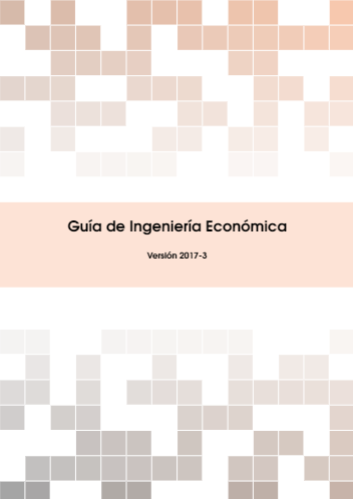
\includegraphics[height=9cm]{W_Varios/1_Portada_libro/gingeco.PNG}

\vspace{4mm}

\vspace{2mm}
\noindent Esta guía fue realizada basada en el libro 'Ingeniería Económica' Octava Edición de Guillermo Baca Currea con el propósito de promover el aprendizaje de los temas pertinentes tratados en este texto en cualquier individuo que desee formarse en ellos. \\
\line(1,0){450}
\vspace{2mm} La protección del derecho de autor abarcará las expresiones pero no las ideas, procedimientos, métodos de operación o conceptos matemáticos en sí.% License information
\noindent \textit{Edición 2022-3}

\clearpage

\chapterimage{ima1} % Table of contents heading image
%\chapterimage{chapter_head_1.pdf} % Table of contents heading image
\pagestyle{empty} % No headers
\tableofcontents % Print the table of contents itself
\cleardoublepage % Forces the first chapter to start on an odd page so it's on the right
\pagestyle{fancy} % Print headers again
\graphicspath{ {img/} }%imágenes de los capítulos, encabezado y background

%-----------------------------------------------------------
%              TABLA DE NOMENCLATURA
%------------------------------------------------------
\graphicspath{ {W_Varios/0_Tablas_notacion/img/ejemplos/}, {img/} }
\begin{center}
	\section*{i. Tabla de nomenclatura }
	\addcontentsline{toc}{section}{i. Tabla de nomenclaturas }
\end{center}

\begin{spacing}{1}
	\begin{center}
		\begin{tabular}{ |p{2.5cm}|p{9.5cm}|}
			\hline
			\rowcolor{orange!50}
			\begin{center} \textbf{Siglas} \end{center} & \begin{center}

				\textbf{Nombre}\end{center}                                                           \\ \hline
			
			EA                        & Efectivo Anual (tasa de referencia SuperFinanciera-nominal anual año vencido- naav) \\ \hline
			
			g                         & Gradiente geométrico                                                                \\ \hline
			
			H                         & Valor incremento escalón monetario                                                  \\ \hline
			
			I                         & Monto de interés                                                                    \\ \hline
			
			IPC                       & Índice de precios al consumidor                                                     \\ \hline
			
			L                         & Gradiente aritmético monetario                                                      \\ \hline
			
			$i$                       & Tasa de interés periódico                                                           \\ \hline
			
			$j$                       & Tasa de interés periódica anualizada                                                \\  \hline
			
			i$_{d}$                   & Tasa periódica de devaluación                                                       \\ \hline
			i$_{f}$                   & Tasa periódica de la inflación                                                      \\ \hline
			i$_{r}$                   & Tasa periódica real                                                                 \\ \hline
			
			m$_{1}$                   & Número de períodos anuales para  i$_{1}$                                            \\ \hline
			
			m$_{2}$                   & Número de períodos anuales para  i$_{2}$                                            \\ \hline
			
			n                         & Número de periodos asociados a una i                                                \\ \hline
			
			na(120d)v                 & Nominal anual (120 días) vencido                                                    \\ \hline
			
			naaa                      & Nominal anual (año) anticipado                                                      \\ \hline
			
			naav                      & Nominal anual (año) vencido                                                         \\ \hline
			
			nasa                      & Nominal anual (semestre) anticipado                                                 \\\hline
			
			nasv                      & Nominal anual (semestre) vencido                                                    \\\hline
			
			nata                      & Nominal anual (trimestre) anticipado                                                \\ \hline
			
			natv                      & Nominal anual (trimestre) vencido                                                   \\ \hline
			
			na(5a)a                   & Nominal anual (5 años) anticipado                                                   \\ \hline
			
			na(5a)v                   & Nominal anual (5 años) vencido                                                      \\ \hline
			
			na(120d)a                 & Nominal anual (120 días) anticipado                                                 \\ \hline
			
			p(120d)v                  & Periódico (120 días) vencido                                                        \\ \hline
			
			paa                       & Periódico (año)  anticipado                                                         \\ \hline
			
			pav                       & Periódico (año) vencido                                                             \\ \hline
			
			psa                       & Periódico (semestre) anticipado                                                     \\\hline
			
			psv                       & Periódico (semestre) vencido                                                        \\\hline
			
			pta                       & Periódico (trimestre) anticipado                                                    \\ \hline
			
			ptv                       & Periódico (trimestre) vencido                                                       \\ \hline
			
			p(5a)a                    & Periódico (5 años) anticipado                                                       \\ \hline
			
			p(5a)v                    & Periódico (5 años) vencido                                                          \\ \hline
			
			p(120d)a                  & Periódico (120 días) anticipado                                                     \\ \hline
			
			R                         & Cuotas seriales fijas                                                               \\ \hline
			
			SPREAD                    & Tasa de interés que se adiciona a una tasa de referencia                            \\ \hline
		\end{tabular}
	\end{center}
\end{spacing}
\ \ \
%\begin{center}
%\section*{Aceptaciones Bancarias}
%\addcontentsline{toc}{section}{Tabla resumen de fórmulas }
%\end{center}
\\ \\ \\ \\ \\ \\ \\
\begin{center} \textbf {Aceptaciones Bancarias (capítulo 3)}\\ \end{center}

\begin{spacing}{1}
	\begin{center}
		\begin{tabular}{ |p{2.5cm}|p{9.5cm}|}
			\hline
			\rowcolor{orange!50}
			\begin{center}\textbf{Siglas} \end{center} & \begin{center} \textbf{Nombre} \end{center}                                                                                                                                                                                                           \\ \hline
			
			
			COM$_{v}$                 & Comisión de Venta del Corredor                                                                                                                                                                                                      \\ \hline
			i$_{c}$                   & Tasa de compra                                                                                                                                                                                                                      \\ \hline
			i$_{R}$                   & Tasa de registro en Bolsa de Valores                                                                                                                                                                                                \\ \hline
			i$_{v}$                   & Tasa de venta                                                                                                                                                                                                                       \\ \hline
			P$_{c}$                   & Precio del comprador                                                                                                                                                                                                                \\ \hline
			P$_{R}$                   & Precio de registro                                                                                                                                                                                                                  \\ \hline
			P$_{v}$                   & Precio de venta                                                                                                                                                                                                                     \\ \hline
			$*$                       & Para las ecuaciones de valor el * es un operador que multiplica o desplaza un flujo y/o el resultado del flujo de series uniformes y/o gradiantes diferidos y/o con tiempo muerto (único caso de uso de este operador en esta guía. \\ \hline
		\end{tabular}
	\end{center}
\end{spacing}



\begin{center} \textbf {Operadores lógicos} \end{center}

\begin{spacing}{1}
	\begin{center}
		\begin{tabular}{ |p{2.5cm}|p{9.5cm}|}
			\hline
			\rowcolor{orange!50}
			\begin{center}\textbf{Siglas} \end{center} & \begin{center} \textbf{Nombre} \end{center}                                 \\ \hline
			
			$ Q \Leftarrow P $        & "Q dado que P", "Q si P", "Q siempre que P"               \\ \hline
			
			$ P \Rightarrow Q $       & "P implica Q", "Si P, entonces Q", "P sólo si Q"          \\ \hline
			
			$ P \Leftrightarrow Q $   & "P si y sólo si Q", "P es necesario y suficiente para Q", 
			"P es equivalente con Q"                                                              \\ \hline
			
			$ \therefore P $         & "Porque P"                                                \\ \hline
			
			$ \therefore  P $         & "Por lo tanto, P"                                         \\ \hline
			
			$\equiv$                  & Equivalente                                               \\ \hline
		\end{tabular}
	\end{center}
\end{spacing}
\newpage
%-----------------------------------------------------------
%              TABLA DE FORMULAS
%------------------------------------------------------

\begin{center}
	\section*{ii. Tabla resumen de fórmulas}
	\addcontentsline{toc}{section}{ii. Tabla resumen de fórmulas trabajadas en la guía}
\end{center}

\begin{spacing}{1}
	\begin{center}
		\begin{tabular}{ |p{7cm}|p{7cm}|}
			\hline
			\rowcolor{orange!50}
			
			\begin{center}\textbf{Fórmula} \end{center}                                                                   & \begin{center} \textbf{Nombre} \end{center}                                 \\ \hline
			
			$(1 + i_{1})^{m_1} = (1 + i_{2})^{m_2}$                                                      & Equivalencia de tasas periódicas                           \\\hline
			
			$i_{r} = i_{1} + i_{2} + i_{1}i_{2}$                                                         & Tasa de interés periódica real                             \\ \hline
			$i_r = \frac{i - i_f}{1 + i_f}$                                                              & Tasa de interés real                                       \\ \hline
			
			$j = im$                                                                                     & Tasa interés nominal anual vencida                         \\ \hline
			
			
			$i_a = \frac{i}{1 + i}$                                                                      & Tasa de interés periódica anticipada                       \\ \hline
			
			$i = \frac{i_a}{1 - i_a}$                                                                    & Tasa de interés periódica vencida                          \\ \hline
			$D = Fdn$                                                                                    & Valor de descuento dado un flujo (F)                       \\ \hline
			
			$F = P(1 + i)^n$                                                                             & Valor futuro                                               \\ \hline
			
			$VP = R  \frac{1-(1 + i)^{-n}}{i} $                                                          & Valor presente serie uniforme vencida                      \\ \hline
			
			$VP_{a} = R  \frac{1-(1 + i)^{-n}}{i}  (1 + i) $                                             & Valor presente serie uniforme anticipada                   \\ \hline
			
			$VF = R  \frac{(1 + i)^n-1}{i} $                                                             & Valor futuro serie uniforme vencida                        \\ \hline
			$VF_{a} = R  \frac{(1 + i)^n-1}{i}(1 + i) $                                                  & Valor futuro serie uniforme anticipada                     \\ \hline
			
			$VP = \frac{R}{i}$                                                                           & Valor presente serie perpetua vencida                      \\ \hline
			$VP = R  \frac{1-(1 + i)^{-n}}{i} + \frac{L}{i}[ \frac{1-(1 + i)^{-n}}{i} - n(1 + i)^{-n} ]$ & Valor presente de gradiente aritmético                     \\ \hline
			$VF = R  \frac{(1 + i)^{n} - 1}{i} + \frac{L}{i}[ \frac{(1 + i)^n - 1}{i} - n ]$             & Valor futuro de gradiente aritmético                       \\ \hline
			$VP = \frac{R}{i} + \frac{L}{i^2}$                                                           & Valor presente gradiente aritmético infinito               \\ \hline
			$VP = R  \frac{(1 + g)^n  (1 + i)^{-n}-1}{g - i} $                                           & Valor presente de gradiente geométrico, si $g \neq i$      \\ \hline
			$VP = \frac{Rn}{1 + i}$                                                                      & Valor presente gradiente geométrico si $g = i$             \\ \hline
			$VF = R  \frac{(1 + g)^n - (1 + i)^n}{g - i} $                                               & Valor futuro gradiente geométrico si $g \neq i$            \\ \hline
			$VF = Rn(1 + i)^{n-1} $                                                                      & Valor futuro gradiente geométrico si $g = i$               \\ \hline
			$VP = \frac{R}{1 - g} $                                                                      & Valor presente gradiente geométrico infinito si $g < i$    \\ \hline
			$VP = \infty $                                                                               & Valor presente gradiente geométrico infinito si $g \geq i$ \\ \hline
		\end{tabular}
		
		\clearpage
		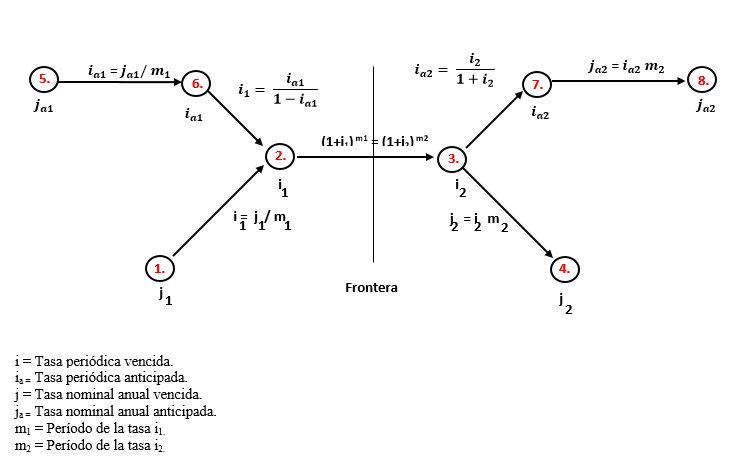
\includegraphics[width = 10.0 cm]{general}\\
		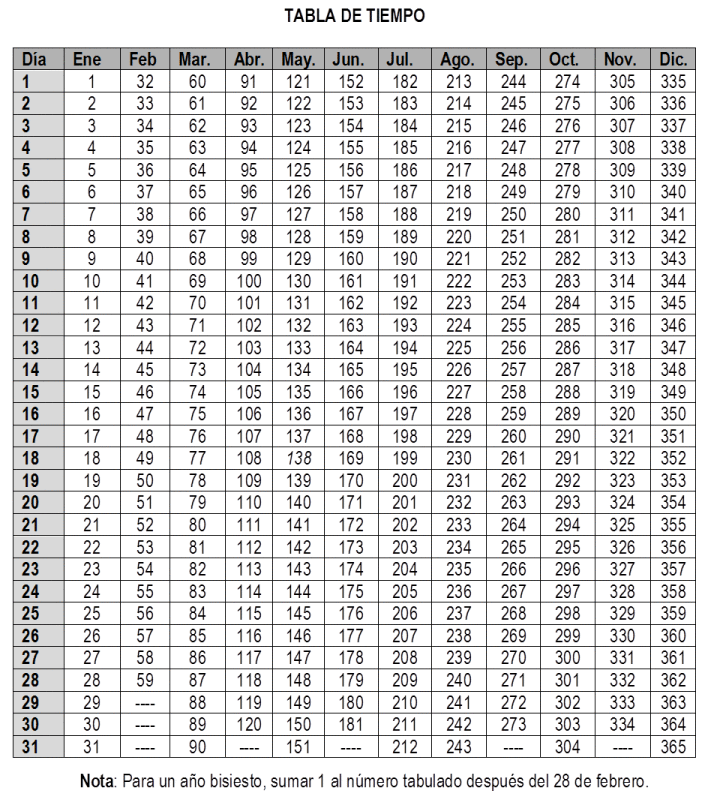
\includegraphics[height=15cm]{TTime}
	\end{center}
\end{spacing}

\clearpage

\begin{center}
	\section*{iii. Tabla resumen de fórmulas}
	\addcontentsline{toc}{section}{iii. Tabla funciones de Excel}
\end{center}

\vspace{2cm}

\begin{spacing}{1}
	\begin{center}
		\begin{tabular}{ |p{7cm}|p{5.5cm}|}
			\hline
			\rowcolor{orange!50}
			
			\begin{center}\textbf{Nombre} \end{center}             & \begin{center} \textbf{Función Financiera en Excel} \end{center} \\ \hline
			
			Equivalencia de tasas periódicas       & TASA(m;;-1;1+i)            \\\hline
			
			Tasa interés nominal anual vencida     & TASA.NOMINAL(i;m)          \\ \hline
			
			Tasa interés periódica año vencido     & INT.EFECTIVO(j;m)          \\ \hline
			
			Valor futuro                           & VF(i;n;;VA,0)              \\ \hline
			
			Valor presente                         & VA(i;n;;VF,0)              \\ \hline
			
			Valor presente serie uniforme vencida  & VNA(i;R1;R2;R3;...)        \\ \hline
			
			Valor futuro serie uniforme vencida    & VF(i;n;;VA,0)              \\ \hline
			
			Valor futuro serie uniforme anticipada & VF(i;n;;VA,1)              \\ \hline
			
			Valor presente serie perpetua vencida  & VA(i;n;R;0)                \\ \hline
			
			Valor presente gradiente aritmético    & VNA(i;R1;R2;R3;...)        \\ \hline
			
			Valor presente gradiente geométrico    & VNA(i;R1;R2;R3;...)        \\ \hline
			
			Valor cuota serie uniforme vencida     & PAGO(i;n;P;F;0)            \\ \hline
			
			Valor cuota serie uniforme anticipada  & PAGO(i;n;P;F;1)            \\ \hline
			
			Ecuación de valor                      & Función Buscar Objetivo    \\ \hline
		\end{tabular}
	\end{center}
\end{spacing}

\clearpage

\graphicspath{ {0_Capitulo/img/ejercicios/}, {W_Varios/2_Portada_capitulos} }

\section*{\textcolor{Blue}{iii. Guía para resolver ejercicios de Ingeniería Económica a partir de la evaluación conceptual}}
\addcontentsline{toc}{section}{iii. Guía para resolver ejercicios de Ingeniería Económica}
\begin{enumerate}
	\item Leer y precisar el enunciado del ejercicio, resaltando las variables independientes, dependientes y los elementos constitutivos para el flujo de caja o diagrama de equivalencia.
	\item Volver a leer para determinar los bloques conceptuales(ejemplo: serie  uniforme proyectada y diferida)
	\item A partir de los bloques determinar primero los subindices de n, luego determinar subindices de valores o series que corresponden a las n.
	\item Estructurar la solución en forma ordenada en 5 pasos: Diagrama de flujo de caja o de equivalencia, declaración de variables, declaración de fórmulas, desarrollo matemático (ECUACIÓN DE VALOR o de equivalencia), respuesta (justificación).
	      \textcolor{Blue}{\item \textbf{Construir el diagrama de flujo de caja, mediante:}}
	      \begin{itemize}
		      \color{Blue}
		      \item Un plano cartesiano, para n períodos vencidos o anticipados según el caso y para el actor de referencia (prestamista o prestatario).
		      \item El dibujo de los egresos en sentido negativo del eje y, y los ingresos en sentido positivo del eje y.
		      \item A la existencia de egresos habrá un ingreso o varios ingresos para poder existir una ecuación de valor.
		      \item Una línea horizontal u oblicua que una el flujo final al flujo inicial de la serie uniforme o serie escalonada o gradiente.
		      \item Una período focal (pf) al final o al comienzo o al intermedio del eje x, que permita visualizar y registrar la ECUACIÓN DE VALOR en el desarrollo matemático.
		      \item Los bucles que direccione el sentido positivo (valor futuro) o negativo (valor presente) del valor de equivalencia con respecto a la período focal.
		      \item Los bucles, en su interior, indicar la i\% o la j\% y el n(número de períodos positivos - valor futuro-, negativos - valor presente) a \underline{trasladar a la derecha o izquierda} el componente de la ecuación de valor. Ante la existencia de ``períodos de gracia'' en series, gradientes, cambios de tasas u otros, no olvidar ``trasladar'' el VP o VF de la serie, gradiente, etc, a la pf mediante el operador fundamental $P=F(1+i)^{-n}$ o $P=F(1+i)^{n}$, según el caso.
		      \item La tasa periódica porcentual (i\%) o la tasa periódica anualizada (j\%) de los bucles vencida o anticipada según la modalidad de los períodos. IMPORTANTE: la periodicidad y modalidad de la tasa de interés (i\%) debe ser igual a las de los períodos (n). En su defecto, utilizar la fórmula de conversión de tasas (i\%) y/o de cambio de modalidad (ia\% a i\%).
	      \end{itemize}
	\item Declarar las variables, mediante el registro de:
	      \begin{itemize}
		      \item Las variables independientes, indicando las unidades de cada una, la periodicidad y modalidad de liquidación de intereses y períodos.
		      \item La variable o variables dependientes, indicando las unidades y el signo de interrogación.
		      \item La verificación de las variables necesarias para la aplicación de las fórmulas.
	      \end{itemize}
	\item Declarar las fórmulas, indicando:
	      \begin{itemize}
		      \item Las fórmulas transitorias y las fundamentales a utilizar, acompañadas del NOMBRE de la misma.
	      \end{itemize}
	      \textcolor{Blue}{\item \textbf{Desarrollar el procedimiento matemático, efectuando:}}
	      \begin{itemize}
		      \color{Blue}
		      \item El remplazo matemático de las fórmulas e indicando las unidades correspondientes.
		      \item El registro de la expresión de ECUACIÓN DE VALOR o equivalencia al remplazo matemático correspondiente.
		      \item El proceso matemático en forma ordenada, clara y precisa. \\
	      \end{itemize}
	\item Registrar la respuesta (justificación), indicando:
	      \begin{itemize}
		      \item La variable independiente o variables independientes, su respuesta y unidades. \\
	      \end{itemize}
\end{enumerate}

\textcolor{Blue}{\textbf{IMPORTANTE 1:}} Volver a leer el enunciado del ejercicio para reconfirmar la respuesta y la justificación. \textbf{\textcolor{ForestGreen}{VALIDAR}} el ejercicio utilizando las fórmulas \textcolor{ForestGreen}{ALGEBRÁICAS} de \textcolor{ForestGreen}{EXCEL}, \textbf{\textcolor{ForestGreen}{FÓRMULAS FINANCIERAS}} de \textcolor{ForestGreen}{EXCEL} y \textbf{\textcolor{ForestGreen}{CRYSTAL BALL}}.\\

\textcolor{Blue}{\textbf{IMPORTANTE 2:}} Aplicar los conceptos de la guía INGECO para articular los formatos y herramientas financieras que requiere fondo emprender en sus convocatorias para financiar planes de negocios como modalidad de grado emprendimiento (Acuerdo 38 de 2015 consejo Académico U Distrital)

\section*{\textcolor{ForestGreen}{iv. Guía para resolver ejercicios de Ingeniería Económica a partir de Excel financiero}}
\addcontentsline{toc}{section}{iv. Guía para resolver ejercicios a partir de Excel financiero}

\begin{enumerate}
	\item Leer y precisar el enunciado del ejercicio, resaltando las variables independientes, dependientes y los elementos constitutivos para el flujo de caja o diagrama de equivalencia.
	\item Volver a leer para determinar los bloques conceptuales (ejemplo: serie uniforme proyectada y diferida).
	\item A partir de los bloques determinar primero los subíndices de n, luego determinar subíndices de valores o series que corresponden a las n.
	\item Estructurar la solución en forma ordenada en 5 pasos: Declaración de variables, tabla de flujo de caja o tabla de amortización o capitalización de ser necesario, aplicación de fórmulas financieras en Excel, respuesta (justificación) y gráfica.
	      \textcolor{ForestGreen}{\item \textbf{Declarar variables mediante el registro de:}}
	      \begin{itemize}
		      \color{ForestGreen}
		      \item Las variables independientes, indicando las unidades de cada una, la periodicidad y modalidad de liquidación de intereses y períodos.
		      \item La variable o variables dependientes, indicando las unidades y dejando la celda de estas con un 0.
		      \item La verificación de las variables necesarias para la aplicación de la formula.
	      \end{itemize}
	      \textcolor{ForestGreen}{\item \textbf{Realizar la tabla de flujo de caja de la siguiente forma:}}
	      \begin{itemize}
		      \color{ForestGreen}
		      \item Definir en la columna [1] el número de períodos correspondientes al ejercicio.
		      \item En la columna [2] rellenar con el flujo correspondiente a cada período en la columna [1].
	      \end{itemize}
	      \begin{center}
		      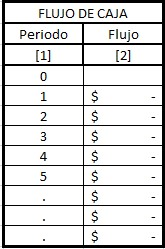
\includegraphics[height=6cm]{0_1}
	      \end{center}
	      
	      En el caso de ser una tabla de amortización se debe rellenar de la siguiente forma:
	      \begin{itemize}
		      \color{ForestGreen}
		      \item Para todos los valores de [3], [4], [5], [6] en el período 0 se les asignara un valor de  COP 0.
		      \item Definir en la columna [1] el número de períodos correspondientes al ejercicio.
		      \item Definir en la columna [2] para el período 1 el valor es igual al rezagado de [6] y arrastrar para todos los períodos.
		      \item Definir en la columna [3] para el período 1 el valor de [1] multiplicado por la celda fija en la que se encuentran los intereses y arrastrar para todos los períodos.
		      \item Definir en la columna [4] para el período 1 el valor de [5] menos el valor de [6] y arrastrar para todos los períodos.
		      \item Definir en la columna [5] el valor de la cuota correspondiente para cada [1] y arrastrar para todos los períodos.
		      \item Definir en la columna [6] el valor de [1] menos el valor de [4] y arrastrar para todos los períodos.
	      \end{itemize}
	      \begin{center}
		      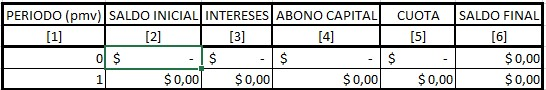
\includegraphics[height=2.35cm]{0_2}
	      \end{center}
	      
	      En el caso de tener una tabla de capitalización de debe rellenar de la siguiente forma:
	      \begin{itemize}
		      \color{ForestGreen}
		      \item Para todos los valores de [1], [2], [3], [4], [5], [6] en el período 0 se les asignara un valor de  COP 0.
		      \item Definir en la columna [1] el número de períodos correspondientes al ejercicio.
		      \item Definir en la columna [2] para el período 1 el valor es igual al rezagado de [5] y arrastrar para todos los períodos.
		      \item Definir en la columna [3] para el período 1 el valor de la cuota correspondiente para cada [1] y arrastrar para todos los períodos.
		      \item Definir en la columna [4] para el período 1 el valor de [2] más el valor [3] multiplicando por la celda fija en la que se encuentran los intereses y arrastrar para todos los períodos.
		      \item Definir en la columna [5] para el período 1 la suma de [2], [3] y [4].
	      \end{itemize}
	      \begin{center}
		      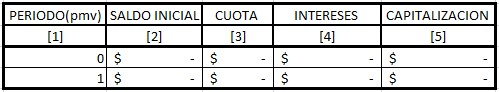
\includegraphics[height=2.5cm]{0_3}
	      \end{center}
	      \textcolor{ForestGreen}{\textbf{NOTA:} Es una buena idea referenciar todos los valores que se apliquen en el flujo de caja desde la declaración de variables, así al cambiar un valor de la declaración de variables cambiará toda la tabla del flujo de caja y de esta forma se puede aplicar análisis de sensibilidad al ejercicio.} \\ \\
	      
	      \textcolor{ForestGreen}{\item \textbf{Para la aplicación de fórmulas financieras en Excel se deberá tener en cuenta cuál fórmula deberá usarse a partir de las siguientes:}} \\
	      
	      
	      \begin{enumerate}
		      \renewcommand{\labelenumi}{\roman{enumi}}
		      \item \textcolor{ForestGreen}{PAGO:} Calcula el pago de un préstamo basado en pagos y tasa de interés constante.
		            \begin{center}
			            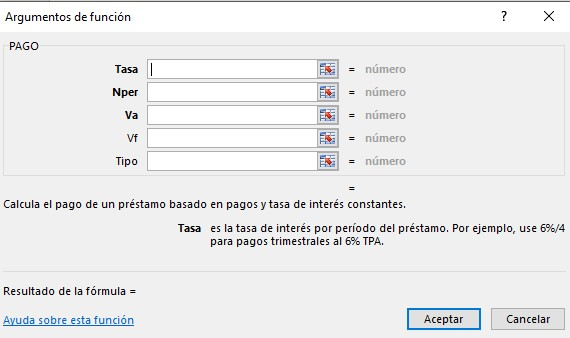
\includegraphics[height=6cm]{0_4} \\
		            \end{center}
		            \begin{center}
			            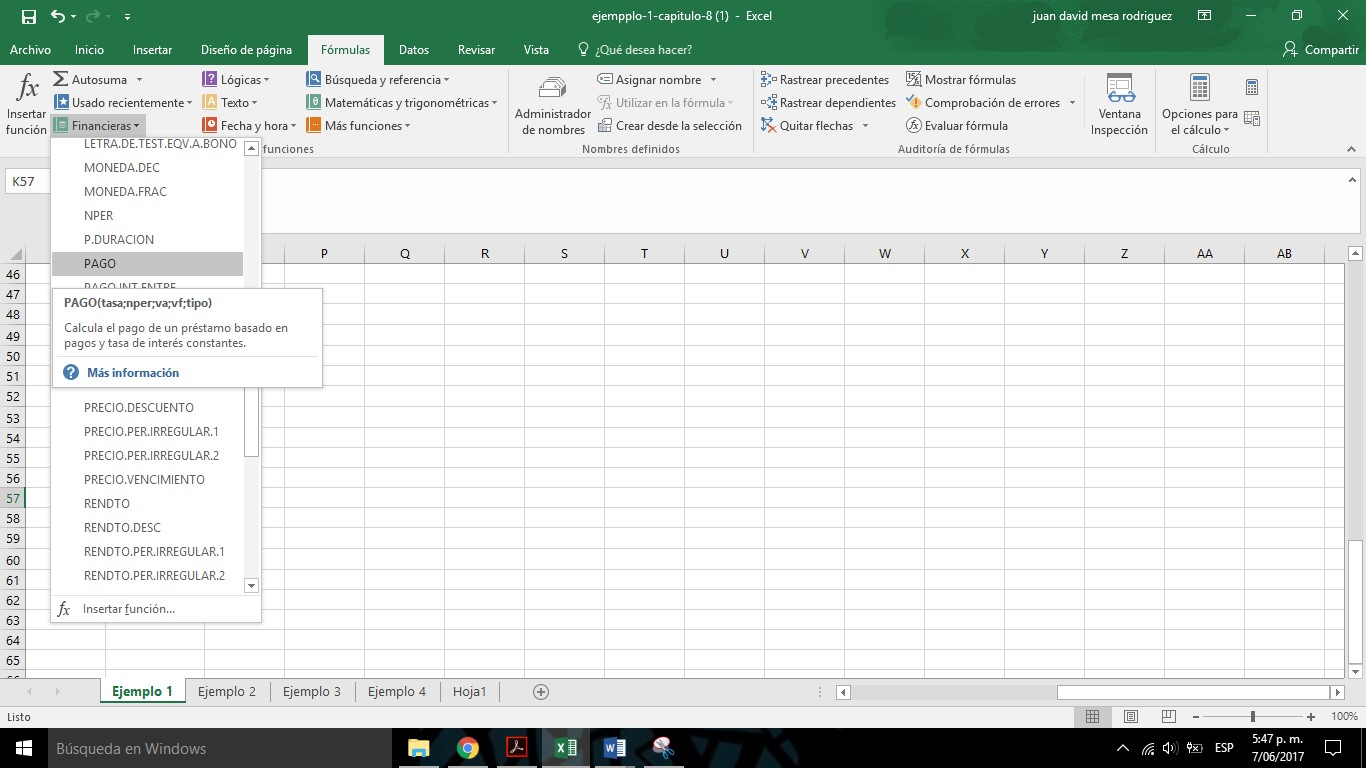
\includegraphics[height=7.41cm]{0_5}
		            \end{center}
		      \item \textcolor{ForestGreen}{VA (Valor actual):} Devuelve el valor presente de una inversión; la suma total del valor actual de una serie de pagos futuros.
		            \begin{center}
			            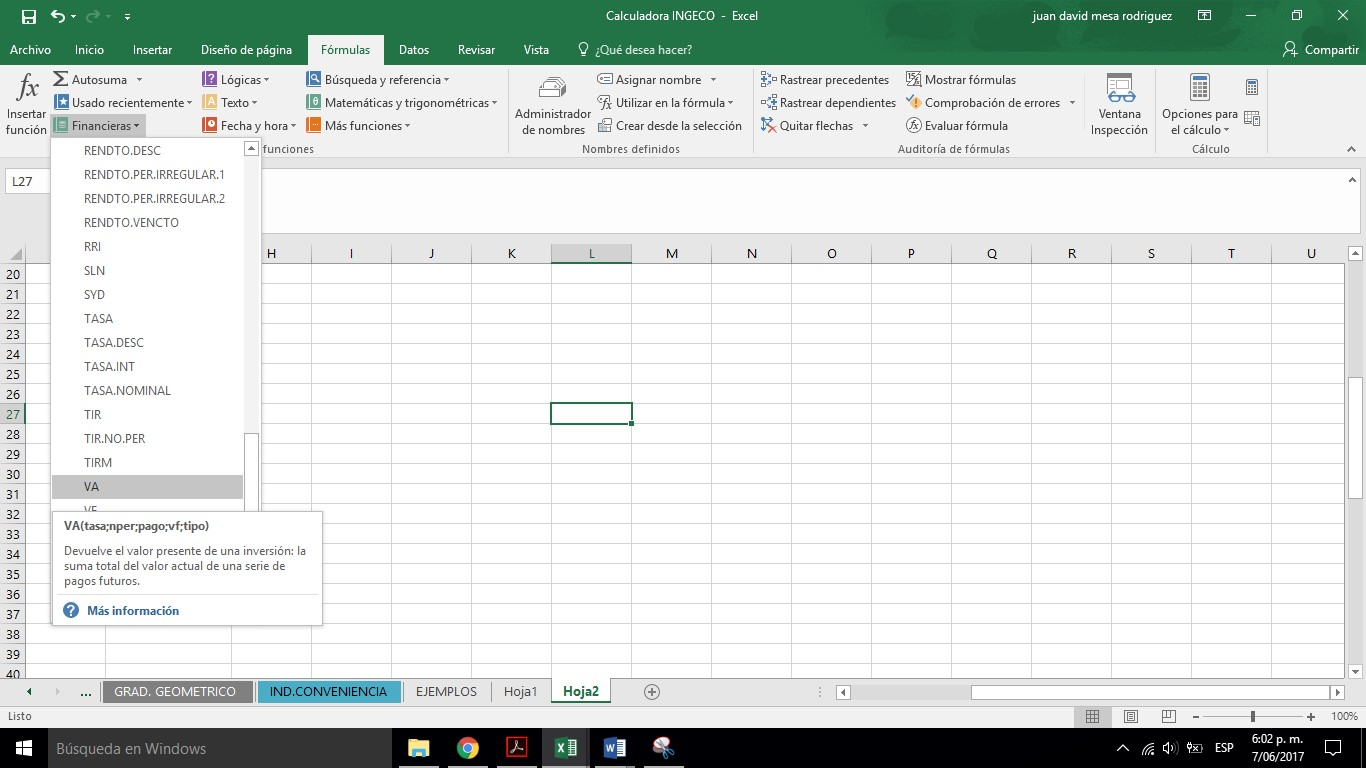
\includegraphics[height=7.41cm]{0_6} \\
		            \end{center}
		            \begin{center}
			            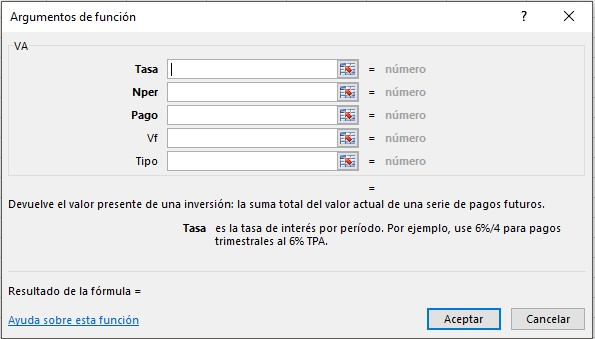
\includegraphics[height=6cm]{0_7}
		            \end{center}
		      \item \textcolor{ForestGreen}{VF (Valor futuro):} Devuelve el valor futuro de una inversión basado en pagos periódicos y constantes, y una tasa de interés también constante.
		            \begin{center}
			            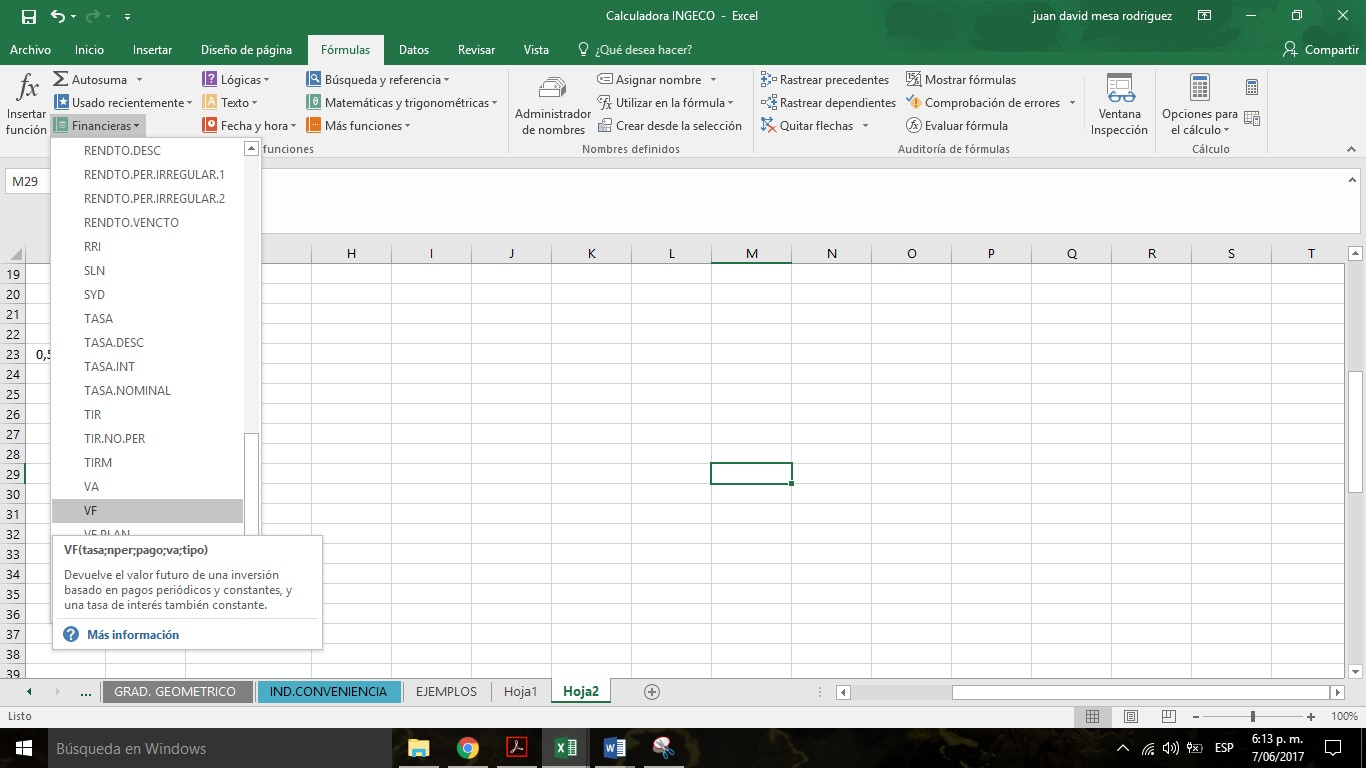
\includegraphics[height=7.15cm]{0_8} \\
		            \end{center}
		            \begin{center}
			            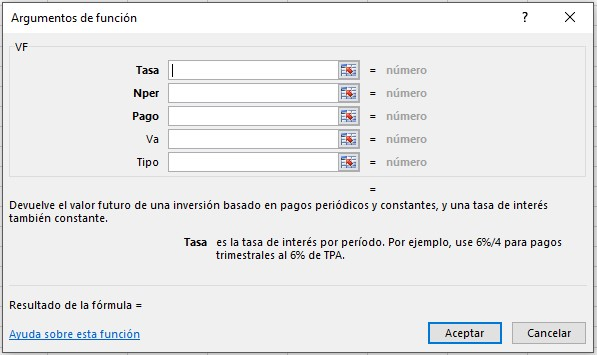
\includegraphics[height=6cm]{0_9}
		            \end{center}
		      \item \textcolor{ForestGreen}{TASA:} Devuelve el valor de la tasa de interés por período de un préstamo o una inversión.
		            \begin{center}
			            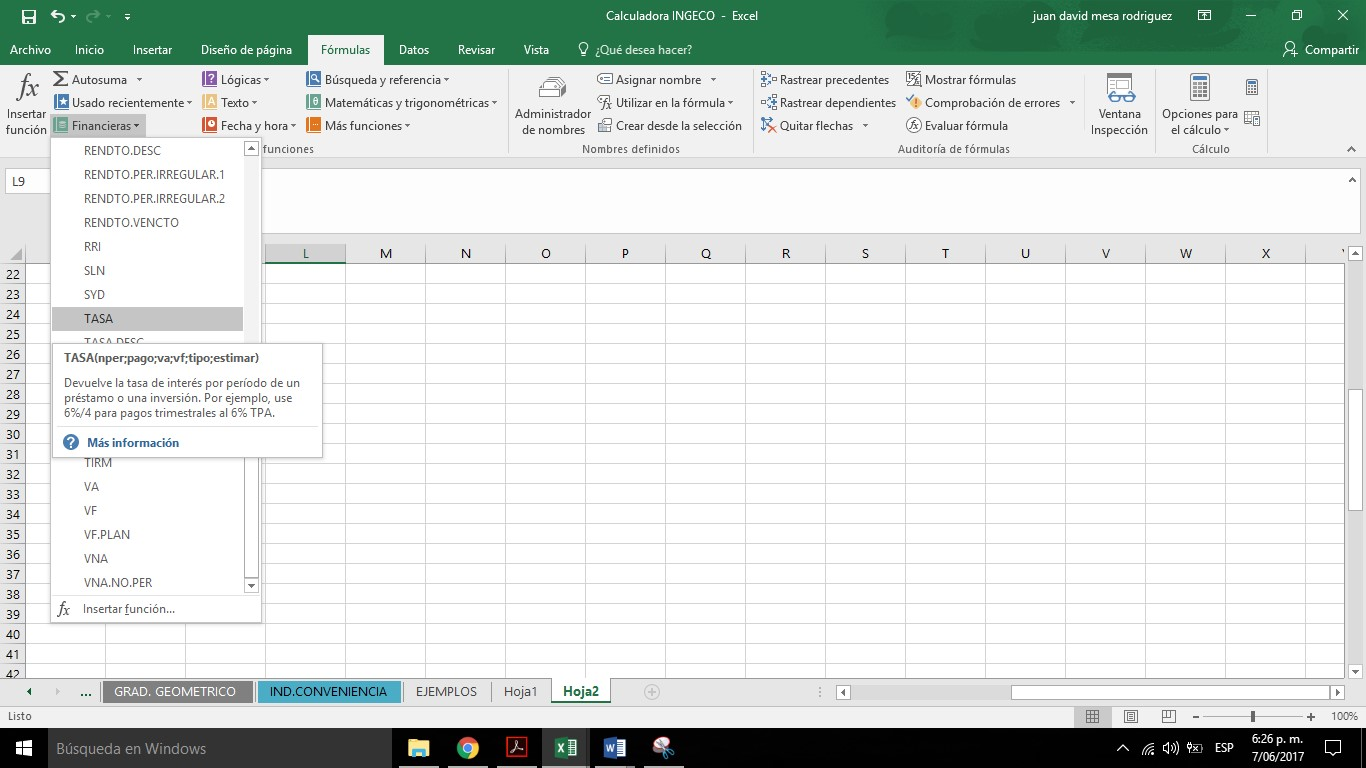
\includegraphics[height=7.15cm]{0_10} \\
		            \end{center}
		            \begin{center}
			            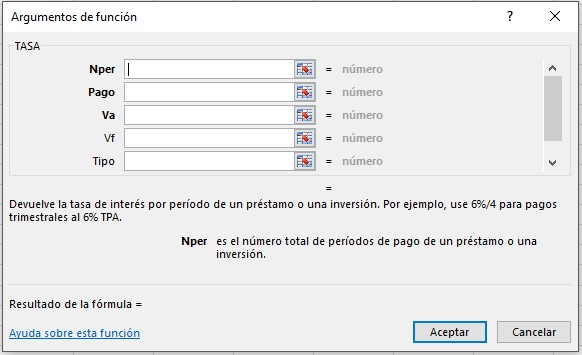
\includegraphics[height=6cm]{0_11}
		            \end{center}
		      \item \textcolor{ForestGreen}{NPER (Numero de períodos):} Devuelve el número de pagos de una inversión, basado en pagos constantes y periódicos y una tasa de interés constante.
		            \begin{center}
			            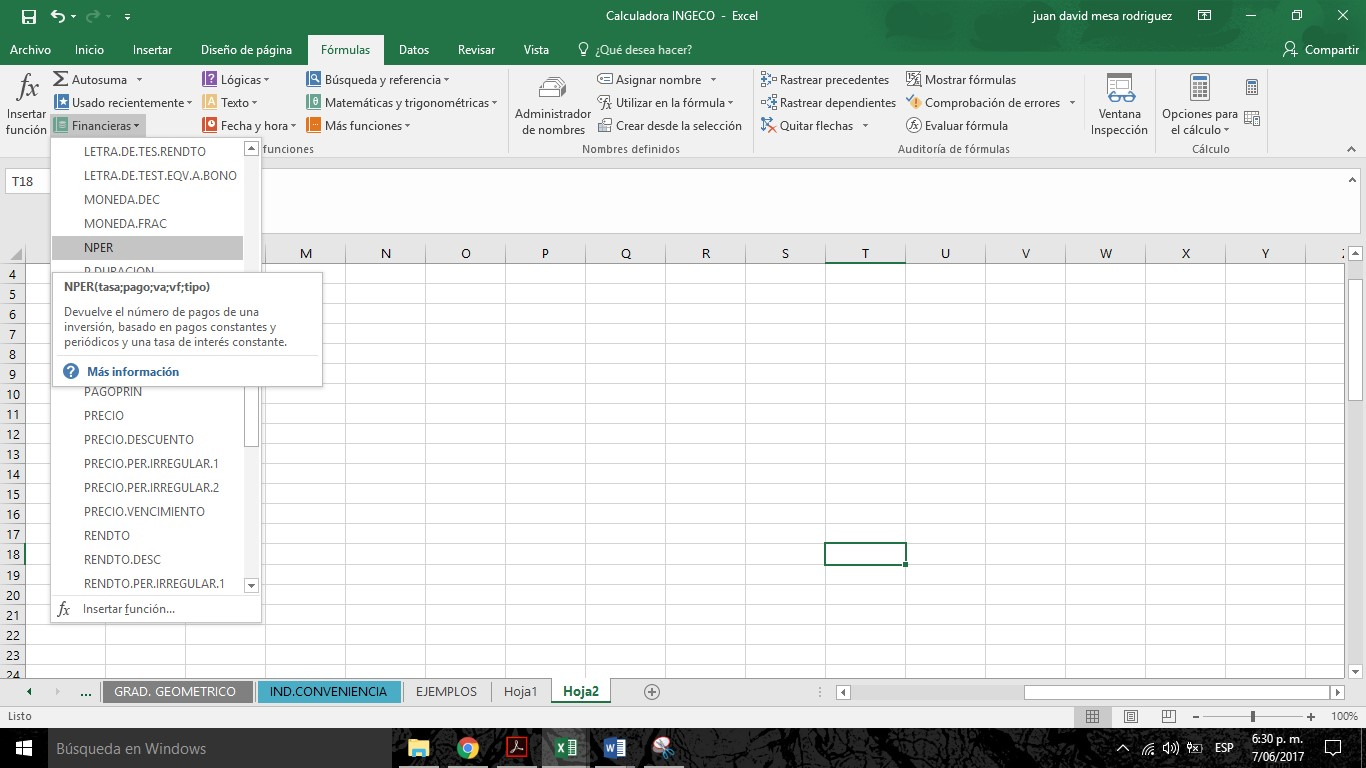
\includegraphics[height=7.15cm]{0_12} \\
		            \end{center}
		            \begin{center}
			            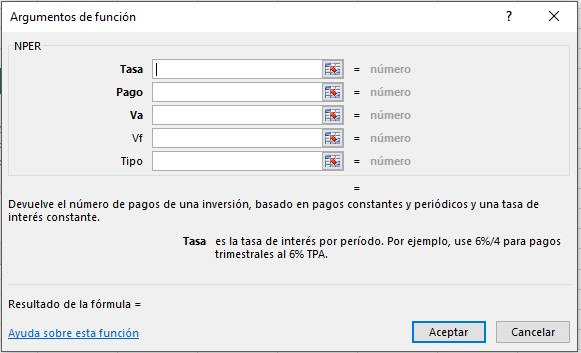
\includegraphics[height=6cm]{0_13}
		            \end{center}
		      \item \textcolor{ForestGreen}{INT. EFECTIVO (Interés efectivo):} Devuelve la tasa de interés anual efectiva.
		            \begin{center}
			            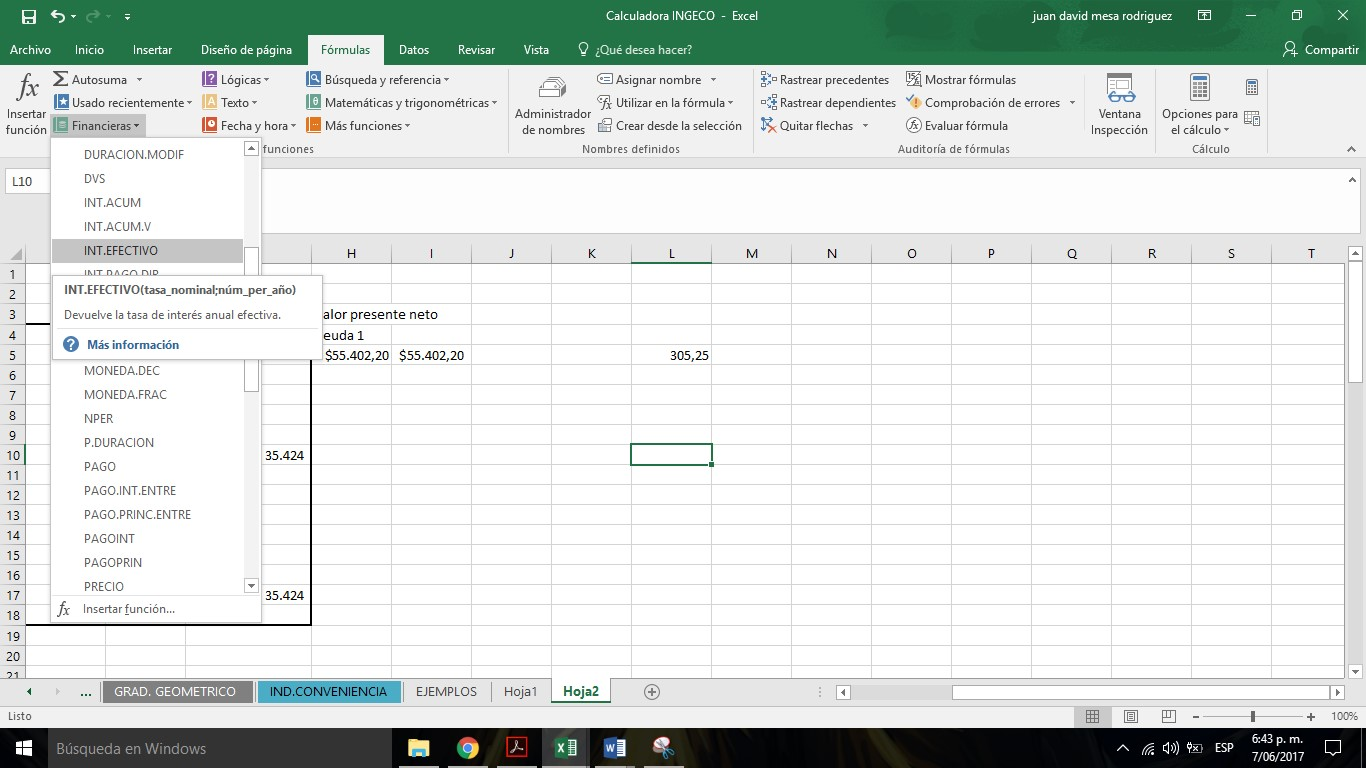
\includegraphics[height=7.15cm]{0_14} \\
		            \end{center}
		            \begin{center}
			            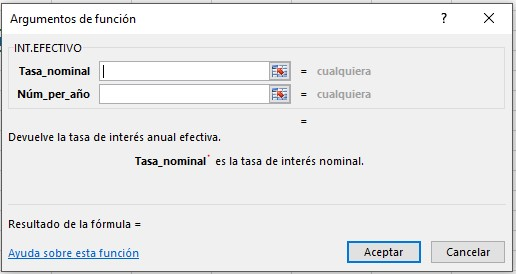
\includegraphics[height=6cm]{0_15}
		            \end{center}
		      \item \textcolor{ForestGreen}{TASA.NOMINAL:} Devuelve la tasa de interés nominal anual.
		            \begin{center}
			            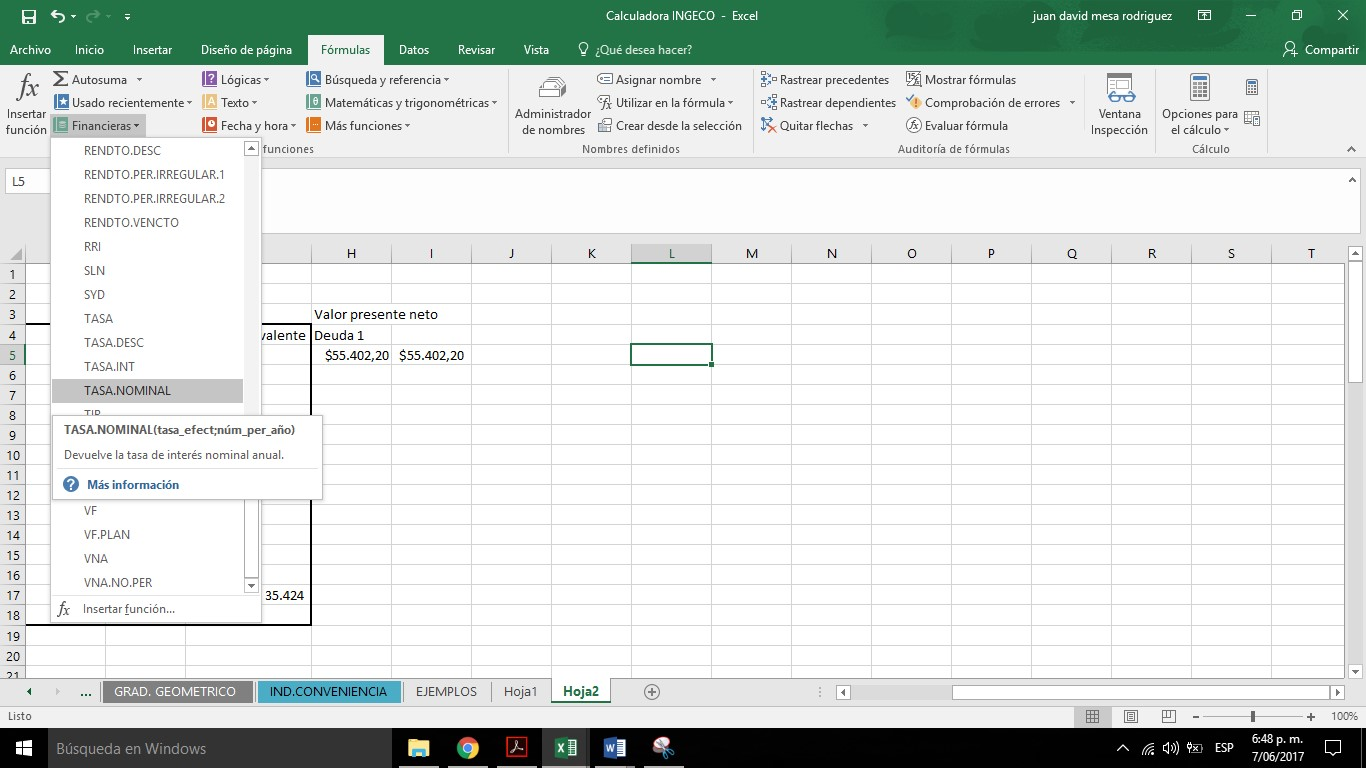
\includegraphics[height=7.15cm]{0_16} \\
		            \end{center}
		            \begin{center}
			            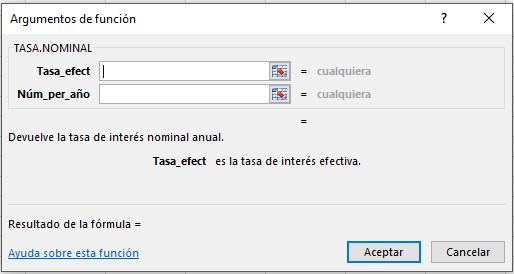
\includegraphics[height=6cm]{0_17}
		            \end{center}
		      \item \textcolor{ForestGreen}{BUSCAR OBJETIVO:} Encuentra la entrada adecuada para el valor que desee.
		            \begin{center}
			            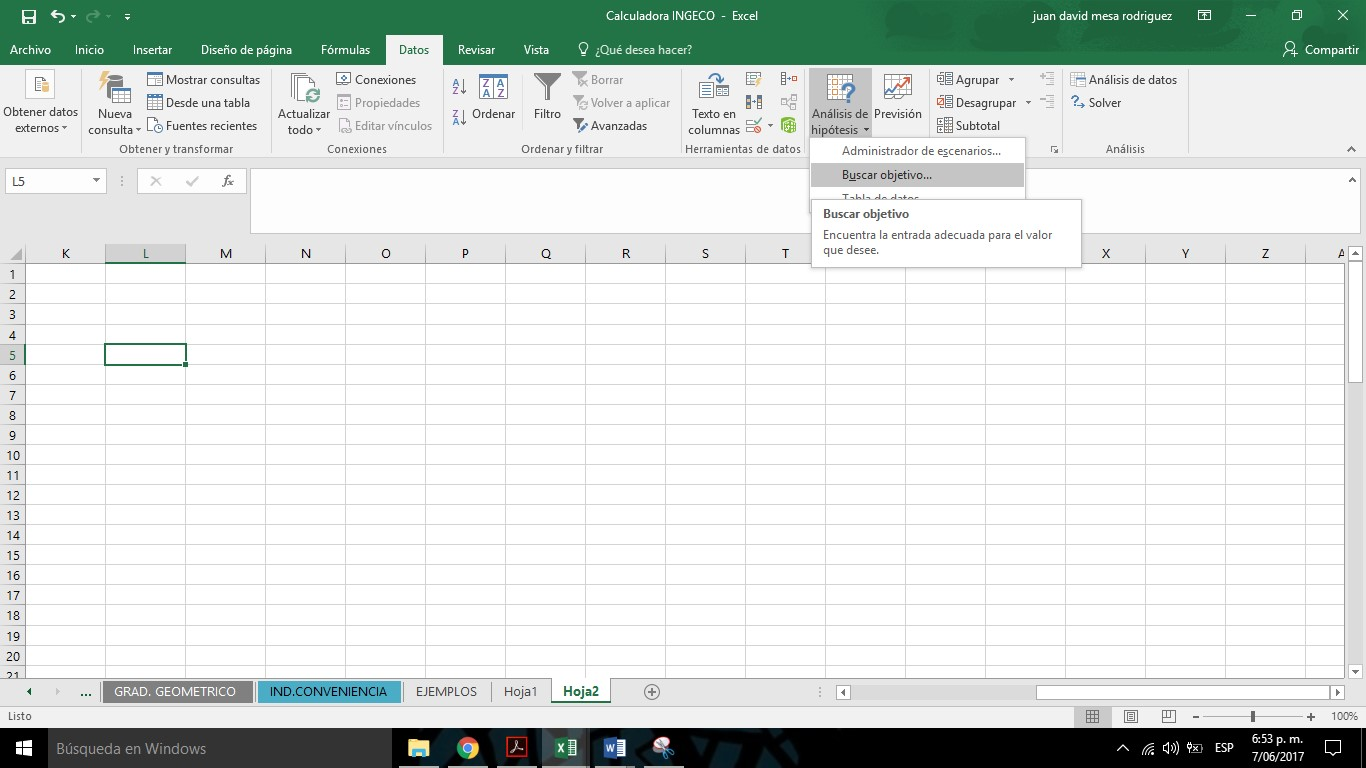
\includegraphics[height=7.15cm]{0_18} \\
		            \end{center}
		            En la opción de \textcolor{ForestGreen}{“Definir la celda”} se debe colocar la celda sobre la que se encuentra la variable sobre la que se conoce el valor que se desea obtener. \\
		            En la opción de \textcolor{ForestGreen}{“Con el valor”} se debe colocar el valor que se desea obtener sobre la variable presente en la opción “Definir la celda”. \\
		            En la opción de \textcolor{ForestGreen}{“Cambiando la celda”} se debe colocar la celda que posee la variable que se desea cambiar para llegar al valor que se encuentra en la opción \textcolor{ForestGreen}{“Con el valor”}. \\
		            Una vez definidas las opciones Excel realizará los cálculos necesarios y devolverá los valores encontrados sobre las celdas colocadas en la fórmula. \\ \\
		            
		            \begin{center}
			            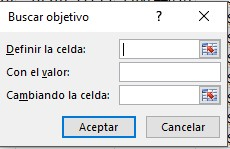
\includegraphics[height=5cm]{0_19}
		            \end{center}
	      \end{enumerate}
	      
	      \textcolor{ForestGreen}{\item \textbf{Registrar la respuesta (justificación) indicando:}}
	      \begin{itemize}
		      \color{ForestGreen}
		      \item La variable independiente o variables independientes, su respuesta y unidades.
	      \end{itemize}
	      
	      \textcolor{ForestGreen}{\item \textbf{Realizar la gráfica correspondiente de la siguiente forma:}}
	      \begin{itemize}
		      \color{ForestGreen}
		      \item La gráfica debe mostrar el comportamiento de los ingresos o egresos a través del número de períodos que posea el problema (Dinero vs Períodos).
		      \item Este debe poseer el título del gráfico, los títulos de los ejes y líneas de cuadrícula.
		      \item Se debe especificar las unidades que posee cada eje.
	      \end{itemize}
	      
	      
\end{enumerate}

\part{Capítulo uno}
\graphicspath{ {1_Capitulo/img/portada/},{1_Capitulo/img/explicacion/},{1_Capitulo/img/ejemplos/} }

%----------------------------------------------------------------------------------------
%	CHAPTER 1
%----------------------------------------------------------------------------------------

\chapterimage{portada.jpg} % Chapter heading image

\chapter{Interés simple}
\section{Mapa Mental }
\begin{figure}[h]
	\centering
	\includegraphics[scale=0.5]{"Mapa Mental 1 V1.0.pdf"}
	\caption{Mapa mental interes simple}
\end{figure}
\newpage
\section{Fórmulas de capítulo}

\begin{spacing}{1.5}
	\begin{center}
		\begin{tabular}{ |p{6cm}|p{5cm}| p{4cm}|}
			\hline
			\rowcolor{orange!50}
			\begin{center}\textbf{Fórmula} \end{center} & \begin{center} \textbf{Nombre}\end{center}          & \begin{center} \textbf{Excel} \end{center} \\ \hline
			
			I = Pin                   & Valor interés simple               & TASA.INT(ni;nf;P)         \\ \hline
			
			F = P+I                   & Valor futuro                       & -                         \\ \hline
			
			P= $\frac{F}{1+ni }$      & Valor presente                     & -                         \\ \hline
			
			
			F= P(1+in)                & Valor futuro                       & -                         \\ \hline
			
			P= F(1-dn)                & Valor presente de un flujo futuro  & -                         \\ \hline
			
			F= P/(1-dn)               & Valor futuro de un flujo presente  & -                         \\ \hline
			
			VL= F(1-dn)               & Valor líquido dado un flujo futuro & -                         \\ \hline
		\end{tabular}
	\end{center}
\end{spacing}

\section{Introducción}
En este capítulo daremos definiciones y conceptos básicos utilizados en las finanzas, los cuales serán indispensables para el desarrollo de la guía. Este enfoque analítico nos permite la optimización de los recursos económicos, lo cual viene a ser el objetivo final de esta guía.

\section{Valor del dinero a través del tiempo}
No es lo mismo tener hoy  COP 100{.}000 que tener  COP 100{.}000 dentro de un año, porque lo que hoy se puede hacer con ese dinero es más de lo que se podrá hacer dentro de un año debido a que normalmente todos los artículos suben de precio, por tal motivo cuando se habla de una suma de dinero debe especificarse la fecha o de lo contrario la información es incompleta. Lo anterior se puede expresar en una forma muy simple: El dinero cambia de valor a través del tiempo.
\\\\
El concepto anterior está íntimamente ligado con el concepto de equivalencia que consiste en que, sumas de dinero diferentes en épocas distintas tienen el mismo poder adquisitivo, así por ejemplo si dentro de un año necesito  COP 120{.}000 para hacer lo que hoy hago con  COP 100{.}000 entonces diré que estas sumas son equivalentes en el tiempo.

\section{Interés (I)}

Todos los bienes son susceptibles de ser entregados a otra persona en arriendo y por ello cobrar un canon de arrendamiento, por lo que es posible dar una casa en arriendo y cobrar una suma mensual por el uso de esa casa, también es posible entregar en arriendo un vehículo o una máquina etc. De la misma forma es posible entregar en arriendo un dinero y el canon del arrendamiento del dinero recibe el nombre de interés el cual representaremos por I.
\\\\
Otra forma de ver el concepto de interés es como la retribución económica que devuelve el capital inicial por período transcurrido, de forma tal que compense la desvalorización de la moneda, que cubra el riesgo y que pague el alquiler del dinero como premio al dueño por no haberlo consumido.

\section{Tasa de interés periódico (i)}
Es el porcentaje (\%) que se paga por el alquiler del dinero, lo representaremos por i . Por ejemplo si tengo que pagar  COP 4 de interés por un préstamo de  COP 100 en un año, entonces la tasa de interés será del 4 \% período anual vencido que se puede escribir como 4\% pav y si tengo que pagar 3 centavos por el préstamo de  COP 1 la tasa será  3\% pav o equivalente a 0{.}03 pav.

\section{Período (n)}
Tiempo unitario de liquidación de intereses, puede ser diario, semanal, mensual, bimensual, trimestral, semestral, anual, bianual, entre otros. %El periodo es equivalente = Días de liquidación de Intereses/ Días del año

\section{Capital inicial (P)}
Es la cantidad de dinero que se invierte, también se le conoce con el nombre de principal, valor actual, valor inicial o valor presente y lo representaremos por P.

\section{Postulado básico de las finanzas}
El postulado básico de las finanzas establece que el interés es una función directa que depende de 3 variables: el capital inicial (\textit{mientras más grande sea el capital mayor deberá ser el interés) la tasa (la tasa depende de las fuerzas del mercado, cuando hay escasez de dinero o cuando los precios en general están al alza la tasa será mayor) y del tiempo (mientras más tiempo dure la inversión mayor será el interés}). Ver la tasa EA de la SuperFinanciera.

\section{Fórmula de interés (I)}
De acuerdo con el postulado anterior podemos establecer la siguiente ecuación:
\begin{equation}
	I = Pin \hspace{35pt} \textit{Valor interés simple (I)}
\end{equation}

\section{Gráfica de flujo de caja}
\textit{A fin de facilitar la comprensión de los problemas mediante una gráfica, se ha adoptado la siguiente convención: la línea horizontal representa el tiempo y allí escribiremos las fechas y los períodos de tiempo; de esta línea salen unas flechas hacia arriba y otras hacia abajo, las que están hacia arriba representan ingresos y las que están hacia abajo representan egresos}.

\section{Capital final (F, i, n, P)}
Es el capital inicial más los intereses, también se le denomina monto, valor final, valor futuro, la suma o acumulado y lo representaremos por $F$. De acuerdo a la definición la fórmula será:

\begin{align*}
	F=P+I \hspace{35pt} \textit{Valor futuro de un flujo (P)}     \\
	F= P(1+in)\hspace{35pt} \textit{Valor futuro de un flujo (p)} \\
\end{align*}

\section{Capital inicial (P, i, n, F)}
Si despejamos P de la fórmula del monto se tiene una fórmula equivalente que nos permite calcular el valor inicial o valor presente:

\begin{align*}
	P=\frac{F}{1+in} \hspace{35 pt} \textit{Valor presente}
\end{align*}

%%%%%%%%%%% NO OLVIDAR COLOCAR ESTE COMENTARIO CON EL NUMERO DE EJERCICIO %%%%%%%%%%%%%
%%%%%%%%%%%%%%%%%%%% EJERCICIO 1 %%%%%%
%%%Text bf para negrilla , el \\ es para el salto de linea.
%%%El primer \\ hace un espacio en el texto y el 2 \\ crea otro espacio
%\begin{minipage}{\textwidth}
%	\textbf{Ejemplo 1}\newline
%	¿A qué tasa periódica mes vencida,  COP 30{.}000 se convertirán en  COP 35{.}000 en 6 meses?\\ \\
%	\textbf{Solución.}\\
%	\begin{center}
%
%		\renewcommand{\arraystretch}{1.5}% Margenes de las celdas
%		%Creación de la cuadricula
%		\begin{tabular}{|c|c|c| }
%			%Creamos una linea horizontal
%			\hline
%			%Definimos el color de la primera fila
%			\rowcolor[HTML]{FFB183}
%			%%%%% INICIO ASIGNACIÓN FECHA FOCAL %%%%%%%
%			%%%%%%%%%% INICIO TITULO
%			%Lo que se hace aquí es mezclar las 3 columnas en una sola
%			\multicolumn{3}{|c|}{\cellcolor[HTML]{FFB183}\textbf{1. Asignación período focal}}   \\ \hline
%			%%%%%%%%%% FIN TITULO
%			%%%%% INICIO DECLARACIÓN DE VARIABLES %%%%%%%
%			\multicolumn{3}{|c|}{$pf = 6pmv$} \\ \hline
%			%Definimos el color de la primera fila
%			\rowcolor[HTML]{FFB183}
%			%%%%% INICIO DECLARACIÓN DE VARIABLES %%%%%%%
%			%%%%%%%%%% INICIO TITULO
%			\multicolumn{3}{|c|}{\cellcolor[HTML]{FFB183}\textbf{2. Declaración de variables}}                                                                                   \\ \hline
%			%%%%%%%%%% FIN TITULO
%			%%%%%%%%%% INICIO DE MATEMÁTICAS
%			$F =  COP 35\,000$                                                       & $n = 6 \textit{  pmv}$                                                       & $i =  COP ? pmv$ \\
%			$P =  COP 30\,000$                                                       &                                                                              &               \\ \hline
%			%%%%%%%%%% FIN DE MATEMÁTICAS
%			%%%%% FIN DECLARACIÓN DE VARIABLES
%			
%			
%			%%%%% INICIO FLUJO DE CAJA
%			\rowcolor[HTML]{FFB183}
%			\multicolumn{3}{|c|}{\cellcolor[HTML]{FFB183}\textbf{3. Diagrama de flujo de caja}}                                                                                  \\ \hline
%			%Mezclamos 3 columnas y pondremos el dibujo
%			%%%%%%%%%%%%% INSERCIÓN DE LA IMAGEN
%			\multicolumn{3}{|c|}{ 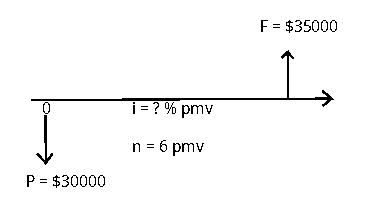
\includegraphics[scale=1.2]{1/capitulo1ejemplo1.pdf} }                                                                                         \\ \hline
%			%%%%%%%%%%%%% FIN INSERCIÓN DE IMAGEN
%			%%%%%FIN FLUJO DE CAJA
%			
%			
%			
%			%%%%% INICIO DECLARACIÓN FORMULAS
%			%%%%%%%%%%% INICIO TITULO
%			\rowcolor[HTML]{FFB183}
%			\multicolumn{3}{|c|}{\cellcolor[HTML]{FFB183}\textbf{4. Declaración de fórmulas}}                                                                                    \\ \hline
%			%%%%%%%%%%% FIN TITULO
%			%%%%%%%%%%% INICIO MATEMÁTICAS
%			
%			$F = P(1+in) \hspace{0.3cm} \textit{Valor futuro}$                   & \multicolumn{2}{c|}{$i = \frac{F}{nP}-\frac{1}{n} \hspace{0.3cm}\textit{Tasa de interés periódica}$}                      \\ \hline
%			%%%%%%%%%% FIN MATEMÁTICAS
%			%%%%%% INICIO DESARROLLO MATEMÁTICO
%			\rowcolor[HTML]{FFB183}
%			%%%%%%%%%%INICIO TITULO
%			\multicolumn{3}{|c|}{\cellcolor[HTML]{FFB183}\textbf{5. Desarrollo matemático}}                                                                                      \\ \hline
%			%%%%%%%%%% FIN TITULO
%			%%%%%%%%%% INICIO MATEMÁTICAS
%			 \multicolumn{3}{|c|}{$i =\frac{ COP 35{.}000}{6\cdot  COP 30{.}000}-\frac{1}{6}=0.2778$}                 \\ \hline
%			%%%%%%%%%% FIN MATEMÁTICAS
%			%%%%%% FIN DESARROLLO MATEMÁTICO
%			
%			\rowcolor[HTML]{FFB183}
%			\multicolumn{3}{|c|}{\cellcolor[HTML]{FFB183}\textbf{6. Respuesta}}    \\ \hline    
%			
%			\multicolumn{3}{|c|}{$i = 2.778\%pmv$} \\ \hline
%		\end{tabular}
%		%Se crean dos lineas en blanco para que no quede el siguiente texto tan pegado
%		\newline \newline
%	\end{center}
%\end{minipage}
%%%%%%%%%%%%%%%%%%%%%%%%%%%FIN EJERCICIO X %%%%%%%%%%%%%%%%%%%%%%%%%%%




\section{Interés anticipado (I$_{a}$)}
El Interés anticipado consiste en cobrar los intereses al principio del período.

\section{Tasa anticipada (d)}
La tasa anticipada es la que genera el interés anticipado y la representaremos por $"d"$, como veremos más adelante también se le denomina tasa de descuento.




%----------------------------------------------------------------------------------------
%	INDEX
%----------------------------------------------------------------------------------------

%----------------------------------------------------------------------------------------

\part{Capítulo dos}
\graphicspath{ {2_Capitulo/img/ejemplos/},{2_Capitulo/img/explicacion/}, {W_Varios/2_Portada_capitulos} }

%----------------------------------------------------------------------------------------
%	CHAPTER 2
%----------------------------------------------------------------------------------------

\chapterimage{2_Capitulo/img/portada/ima2} % Chapter heading image
\chapter{Interés Compuesto}

%------------------------------------------
%Tabla de Fórmulas
%------------------------------------------

\section{Mapa Mental}
\begin{center}
   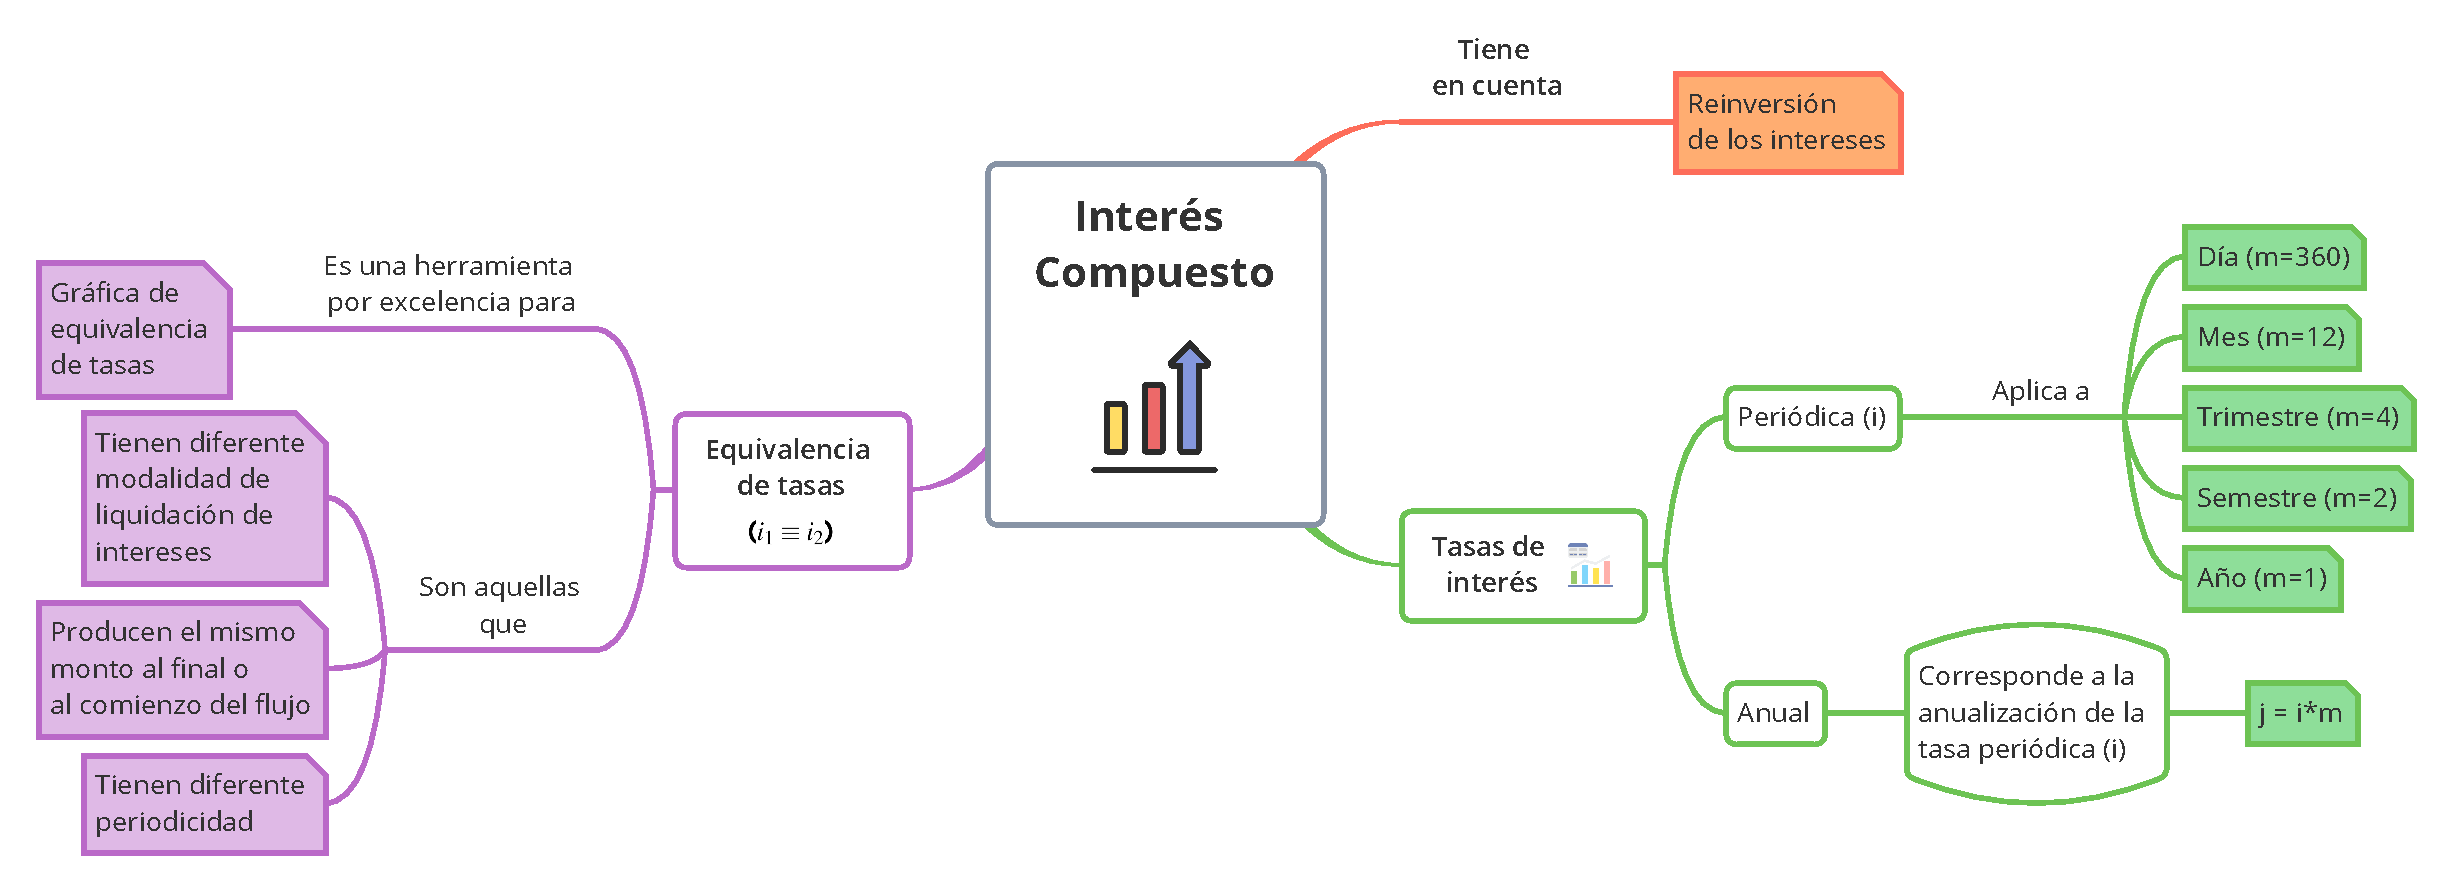
\includegraphics[height = 5.6 cm]{Mapa Mental 2.1.pdf}\\
\end{center}
\clearpage
\section{{Fórmulas del Capítulo}}
\begin{spacing}{1.3}
   \begin{center}
      \begin{tabular}{ |p{4cm}|p{5cm}| p{5cm}|}
         \hline
         \rowcolor{orange!50}
         \begin{center}\textbf{Fórmula} \end{center}   & \begin{center} \textbf{Nombre}\end{center} & \begin{center} \textbf{Excel} \end{center} \\ \hline
         F = $P(1+i)^n$                                & Valor futuro                               & VF(i;n;;VA,0)                              \\ \hline
         P = $\frac{F}{(1 + i)^{n}}$                   & Valor presente                             & VA(i;n;;VF,0)                              \\ \hline
         j = i(m)                                      & Tasa periódica anualizada                  & TASA.NOMINAL(i;m)                          \\ \hline
         ${(1 + i_{1})^{m_1}}$ = ${(1 + i_{2})^{m_2}}$ & Equivalencia de tasas                      & TASA(m;;-1;1+i)                            \\ \hline
      \end{tabular}
   \end{center}
\end{spacing}
\section{Interés compuesto}
Es la acumulación de intereses producidos por un capital inicial a una tasa de interés durante períodos determinados.\\

% ejemplo1
%%%%%%%%%%%%%%%%%%% EJERCICIO 1a %%%%%%

%\newpage %USAR SOLO SI EL SOLUCIÓN QUEDA SOLO Y ES NECESARIO BAJARLO A LA SIGUIENTE PAGINA
\textbf{Solución.}\\
%La tabla ira centrada
\begin{center}
	\renewcommand{\arraystretch}{1.6}% Margenes de las celdas
	%Creación de la cuadricula de 3 columnas
	\begin{longtable}[H]{|c|c|c|}
		%Creamos una linea horizontal
		\hline
		%Definimos el color de la primera fila
		\rowcolor[HTML]{FFB183}
		%%%%% INICIO ASIGNACIÓN PERIODO FOCAL %%%%%%%
		%%%%%%%%%% INICIO TITULO
		%Lo que se hace aquí es mezclar las 3 columnas en una sola
		\multicolumn{3}{|c|}{\cellcolor[HTML]{FFB183}\textbf{1. Asignación período focal}}  \\ \hline
		\multicolumn{3}{|c|}{$pf = \textit{0 ptv}$}   \\\hline
		%%%%%%%%%% FIN TITULO
		%%%%% INICIO DECLARACIÓN DE VARIABLES %%%%%%%
		%%%%%%%%%% INICIO TITULO
		%Lo que se hace aquí es mezclar las 3 columnas en una sola
		\multicolumn{3}{|c|}{\cellcolor[HTML]{FFB183}\textbf{2. Declaración de variables}}   \\ \hline
		%%%%%%%%%% FIN TITULO
		%%%%%%%%%% INICIO DE MATEMÁTICAS
		%Cada & hace referencia al paso de la siguiente columna
		\multicolumn{2}{|c|}{$ \hspace{2 cm} VP= 200.000 \ COP \hspace{2 cm}$}       & $ i  \equiv  8\% \textit{ ptv}$ \\
		\multicolumn{2}{|c|}{$ \hspace{2 cm} j \equiv 32\% \ \textit{natv} \hspace{2 cm}$} & $n=\textit{4 ptv}$ \\
		\multicolumn{2}{|c|}{$ \hspace{2 cm} R = ? COP  \hspace{2 cm}$}              &  \\ \hline
	
		
		%%%%%%%%%% FIN DE MATEMÁTICAS
		%%%%% FIN DECLARACIÓN DE VARIABLES
		
		
		%%%%% INICIO FLUJO DE CAJA
		\rowcolor[HTML]{FFB183}
		\multicolumn{3}{|c|}{\cellcolor[HTML]{FFB183}\textbf{3. Diagrama de flujo de caja}} \\ \hline
		%Mezclamos 3 columnas y pondremos el dibujo
		%%%%%%%%%%%%% INSERCIÓN DE LA IMAGEN
		%Deberán descargar las imágenes respectivas del drive y pegarlas en la carpeta
		%n_capitulo/img/ejemplos/1/capitulo1ejemplo1.pdf  (el /1/ es el numero del ejemplo)
		\multicolumn{3}{|c|}{ 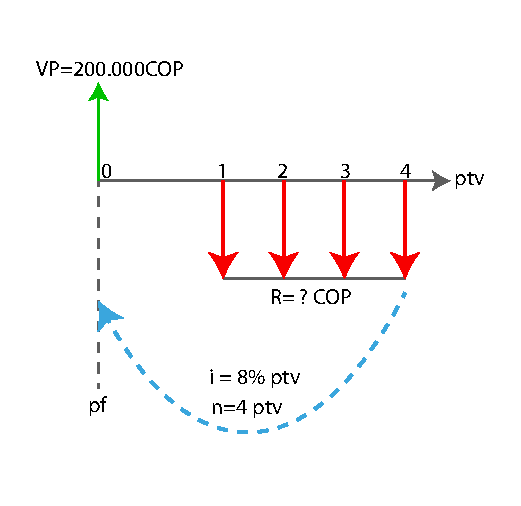
\includegraphics[trim=-78 -5 -78 -5]{7_Capitulo/img/ejemplos/1/Capitulo7-Ejercicio1.pdf} }
		
		
		\\ \hline
		%%%%%%%%%%%%% FIN INSERCIÓN DE IMAGEN
		%%%%%FIN FLUJO DE CAJA
		
		
		
		%%%%% INICIO DECLARACIÓN FORMULAS
		%%%%%%%%%%% INICIO TITULO
		\rowcolor[HTML]{FFB183}
		\multicolumn{3}{|c|}{\cellcolor[HTML]{FFB183}\textbf{4. Declaración de fórmulas}}    \\ \hline
		%%%%%%%%%%% FIN TITULO
		%%%%%%%%%%% INICIO MATEMÁTICAS
		
		\multicolumn{3}{|c|}{$VP=R(\frac{1-(1+i)^{-n}}{i}) \hspace{0.4 cm} \textit{Valor presente de una serie uniforme vencida}$} \\ \hline
		
		%%%%%%%%%% FIN MATEMÁTICAS
		%%%%%% INICIO DESARROLLO MATEMÁTICO
		\rowcolor[HTML]{FFB183}
		%%%%%%%%%%INICIO TITULO
		\multicolumn{3}{|c|}{\cellcolor[HTML]{FFB183}\textbf{5. Desarrollo matemático}}       \\ \hline
		%%%%%%%%%% FIN TITULO
		%%%%%%%%%% INICIO MATEMÁTICAS
		\multicolumn{3}{|c|}{$ 200.000 \ COP=R(\frac {1-(1+0.08)^{-4}} {8\% ptv}) $ \hspace{0.2 cm} $\rightarrow$ \hspace{0.2 cm} $ R= 60.384,16 \ COP $} \\ \hline
		
		%%%%%%%%%% FIN MATEMÁTICAS
		%%%%%% FIN DESARROLLO MATEMÁTICO
		%%%%%% INICIO RESPUESTA
		\rowcolor[HTML]{FFB183}
		%%%%%%%%%%INICIO TITULO
		\multicolumn{3}{|c|}{\cellcolor[HTML]{FFB183}\textbf{6. Respuesta}}   \\ \hline
		%%%%%%%%%% FIN TITULO
		%%%%%%%%%% INICIO RESPUESTA MATEMÁTICA
		\multicolumn{3}{|c|}{$\mathbf{R= 60.384,16 \ COP}$}
		\begin{comment}
		\multicolumn{3}{|p{\textwidth}|}{
		$F_{4} = F_{5} = 21.609,84 \ COP $ .}
		\end{comment} 
		\\ \hline
		%%%%%%%%%% FIN MATEMÁTICAS
		%%%%%% FIN RESPUESTA
	\end{longtable}
	%Se crean dos lineas en blanco para que no quede el siguiente texto tan pegado
	%\newline \newline %USARLO SI CREES QUE ES NECESARIO
\end{center}
%%%%%%%%%%%%%%%%%%%%%%%%%%FIN EJERCICIO 1a %%%%%%%%%%%%%%%%%%%%%%%%%%%

\clearpage

En resumen, se tiene en el inciso A:
\begin{table}[htbp]
   \begin{center}
      \begin{tabular}{|l|l|l|l|}
         \hline
         Período & Capital Inicial & Interés     & Capital Final \\
         \hline
         0       & 200.000 COP &  0 COP      & 200.000 COP  \\ \hline
         1       & 200.000 COP &  20.000 COP & 220.000 COP  \\ \hline
         2       & 200.000 COP &  20.000 COP & 240.000 COP  \\ \hline
         3       & 200.000 COP &  20.000 COP & 260.000 COP  \\ \hline
         4       & 200.000 COP &  20.000 COP & 280.000 COP  \\ \hline
      \end{tabular}
      \label{tabla:interesSimple1}
   \end{center}
\end{table}

%%%%%%%%%%%%%%%%%%% EJERCICIO 1 %%%%%%

%\newpage %USAR SOLO SI EL SOLUCIÓN QUEDA SOLO Y ES NECESARIO BAJARLO A LA SIGUIENTE PAGINA

%La tabla ira centrada
\begin{center}
  \renewcommand{\arraystretch}{1.5}% Margenes de las celdas
  %Creación de la cuadricula de 3 columnas
  \begin{flushleft}\textbf{A.2} \end{flushleft}
  \begin{longtable}[H]{|C{0.3\linewidth}|C{0.3\linewidth}|C{0.3\linewidth}|}
    %Creamos una linea horizontal
    \hline
    %Definimos el color de la primera fila
    \rowcolor[HTML]{FFB183}
    %%%%% INICIO ASIGNACIÓN FECHA FOCAL %%%%%%%
    %%%%%%%%%% INICIO TITULO
    %Lo que se hace aquí es mezclar las 3 columnas en una sola
    \multicolumn{3}{|c|}{\cellcolor[HTML]{FFB183}\textbf{1. Asignación período focal}}  \\ \hline
    %%%%%%%%%% FIN TITULO
    %%%%% INICIO DECLARACIÓN DE VARIABLES %%%%%%%
    \multicolumn{3}{|c|}{$pf = 4ptv$} \\ \hline
    %%%%%%%%%% INICIO TITULO
    %Lo que se hace aquí es mezclar las 3 columnas en una sola
    \multicolumn{3}{|c|}{\cellcolor[HTML]{FFB183}\textbf{2. Declaración de variables}}  \\ \hline
    %%%%%%%%%% FIN TITULO
    %%%%%%%%%% INICIO DE MATEMÁTICAS
    %Cada & hace referencia al paso de la siguiente columna
    
    $P =  200{.}000 COP$  & $i = 10\%\textit{ ptv} $  & $I= ? COP$   \\
      & $n=\frac{360 \textit{días}}{90 \textit{días}} =4 ptv$ & $F= ? COP$
    \\\hline

    %%%%%%%%%% FIN DE MATEMÁTICAS
    %%%%% FIN DECLARACIÓN DE VARIABLES

    %%%%% INICIO FLUJO DE CAJA
    \rowcolor[HTML]{FFB183}
    \multicolumn{3}{|c|}{\cellcolor[HTML]{FFB183}\textbf{3. Diagrama de flujo de caja}}                                                                          \\ \hline
    %Mezclamos 3 columnas y pondremos el dibujo
    %%%%%%%%%%%%% INSERCIÓN DE LA IMAGEN
    %Deberán descargar las imágenes respectivas del drive y pegarlas en la carpeta
    %n_capitulo/img/ejemplos/1/capitulo1ejemplo1.pdf  (el /1/ es el numero del ejemplo)
    \multicolumn{3}{|c|}{ 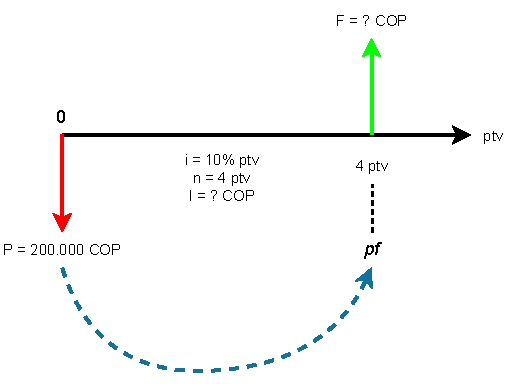
\includegraphics[trim=-5 -5 -5 -5 , scale=1]{2_Capitulo/ejemplos/1/Capitulo2Ejercicio1a2_v2.pdf} }                                         \\ \hline
    %%%%%%%%%%%%% FIN INSERCIÓN DE IMAGEN
    %%%%%FIN FLUJO DE CAJA

    %%%%% INICIO DECLARACIÓN FORMULAS
    %%%%%%%%%%% INICIO TITULO
    \rowcolor[HTML]{FFB183}
    \multicolumn{3}{|c|}{\cellcolor[HTML]{FFB183}\textbf{4. Declaración de fórmulas}}                                                                            \\ \hline
    %%%%%%%%%%% FIN TITULO
    %%%%%%%%%%% INICIO MATEMÁTICAS

    $I = Pin\hspace{0.3cm} \textit{Interés monetario simple}$ & \multicolumn{2}{c|}{$F = P + I \hspace{0.3cm} \textit{Valor futuro}$}                            \\ \hline
    %%%%%%%%%% FIN MATEMÁTICAS
    %%%%%% INICIO DESARROLLO MATEMÁTICO
    \rowcolor[HTML]{FFB183}
    %%%%%%%%%%INICIO TITULO
    \multicolumn{3}{|c|}{\cellcolor[HTML]{FFB183}\textbf{5. Desarrollo matemático}}                                                                              \\ \hline
    %%%%%%%%%% FIN TITULO
    %%%%%%%%%% INICIO MATEMÁTICAS
    $n=4ptv$                                                  & \multicolumn{2}{c|}{}                                                                            \\ $I_{1}= 200{.}000$ COP$\cdot0.1\cdot1$ & \multicolumn{2}{c|}{$F =  200{.}000$ COP + $20{.}000$ COP + $22{.}000$ COP}  \\ $I_{1}=  20{.}000$ COP & \multicolumn{2}{c|}{$+ 24{.}200$ COP + $26{.}620$ COP}  \\
    $I_{2}= 220{.}000\cdot0.1\cdot1$ COP   & \multicolumn{2}{c|}{$F= P+I$} \\
    $I_{2}= 22{.}000$ COP                  & \multicolumn{2}{c|}{$F=200{.}000$ COP$+92{.}820$ COP}   \\
    $I_{3}= 242{.}000\cdot0.1\cdot1$ COP   & \multicolumn{2}{c|}{$F= 292{.}820$ COP}                \\
    $I_{3}= 24{.}200$ COP                  & \multicolumn{2}{c|}{}                                                           \\
    $I_{4}= 266{.}200\cdot0.1\cdot1$ COP   & \multicolumn{2}{c|}{}                                                                            \\
    $I_{4}= 26{.}620$ COP                  & \multicolumn{2}{c|}{}                                                                            \\
    $I= 20{.}000 COP + 22{.}000 COP + 24{.}200 COP + 26{.}620 COP$& \multicolumn{2}{c|}{}                                        \\
    $I= 92{.}820$ COP                      & \multicolumn{2}{c|}{}
    
    \\ \hline
    %%%%%%%%%% FIN MATEMÁTICAS
    %%%%%% FIN DESARROLLO MATEMÁTICO
    %%%%%% INICIO RESPUESTA
    \rowcolor[HTML]{FFB183}
    %%%%%%%%%%INICIO TITULO
    \multicolumn{3}{|c|}{\cellcolor[HTML]{FFB183}\textbf{6. Respuesta}}                                                                                          \\ \hline
    %%%%%%%%%% FIN TITULO
    %%%%%%%%%% INICIO RESPUESTA MATEMÁTICA
    $I= 92{.}820 COP$                                         &
    \multicolumn{2}{c|}{$F= 292{.}820 COP$
    }                                                                                                                                                            \\ \hline
    %%%%%%%%%% FIN MATEMÁTICAS
    %%%%%% FIN RESPUESTA
  \end{longtable}
  %Se crean dos lineas en blanco para que no quede el siguiente texto tan pegado
  %\newline \newline %USARLO SI CREES QUE ES NECESARIO
\end{center}
%%%%%%%%%%%%%%%%%%%%%%%%%%FIN EJERCICIO 1 %%%%%%%%%%%%%%%%%%%%%%%%%%%



Representando en una tabla la información obtenida en el apartado anterior del ejercicio se tiene lo siguiente:\\

\begin{table}[htbp]
   \begin{center}
      \begin{tabular}{|l|l|l|l|}
         \hline
         Período & Capital Inicial & Interés     & Capital Final \\
         \hline
         0 & 200.000 COP & 0 COP      & 200.000 COP \\ \hline
         1 & 200.000 COP & 20.000 COP & 220.000 COP \\ \hline
         2 & 220.000 COP & 22.000 COP & 242.000 COP \\ \hline
         3 & 242.000 COP & 24.200 COP & 266.000 COP \\ \hline
         4 & 266.000 COP & 26.000 COP & 292.000 COP \\ \hline
      \end{tabular}
      \label{tabla:interesCompuesto1}
   \end{center}
\end{table}
\textbf{Generalizando:}\\
\begin{table}[htbp]
   \begin{center}
      \begin{tabular}{|l|l|l|l|}
         \hline
         Período & Capital Inicial & Interés         & Capital Final                                       \\
         \hline
         0       & P               & 0               & $F_{0}$=P                                           \\ \hline
         1       & P               & Pi              & $F_{1}$ = P + Pi = P(1+i)                           \\ \hline
         2       & P(1+i)          & P(1+i)i         & $F_{2}$ = P(1+i) + P(1+i)i = $P(1+i)^{2}$           \\ \hline
         .       & .               & .               & .                                                   \\ \hline
         ..      & ..              & ..              & ..                                                  \\ \hline
         ...     & ...             & ...             & ...                                                 \\ \hline
         n       & $P(1+i)^{n-1}$  & $P(1+i)^{n-1}i$ & $F_{n} = P(1+i)^{n-1} + P(1+i)^{n-1}i = P(1+i)^{n}$ \\ \hline
      \end{tabular}
      \label{tabla:interesCompuesto2}
   \end{center}
\end{table}

Se concluye que la fórmula del interés compuesto es:\\
$F = P(1+i)^n$ \hspace{20 pt} \textit{Valor futuro}\\

\textbf{Volviendo al ejemplo 1:}\\
$F = P(1+i)^n$\\
$F =  200.000 (1+0,1)^4$ COP\\
$F =  292.820$ COP\\

%%%%%%%%%% NO OLVIDAR COLOCAR ESTE COMENTARIO CON EL NUMERO DE EJERCICIO %%%%%%%%%%%%%
%%%%%%%%%%%%%%%%%%% EJERCICIO 2 %%%%%%
%%Text bf para negrilla , el \\ es para el salto de linea.
%%El primer \\ hace un espacio en el texto y el 2 \\ crea otro espacio
\textbf{Ejemplo 2}\newline
El jefe de producción de una fábrica debe decidir entre dos máquinas A y B. Las características de cada una son: \\
\begin{center}
		\begin{tabular}{|p{1cm}|p{2cm}|p{2cm}|p{2cm}|p{3cm}|}
			\hline
			\rowcolor{white!50}
			\textbf{Maq.} & \textbf{C} & \textbf{K} & \textbf{S} & \textbf{CAO} \\ \hline
			A            & 800.000 COP   & 3 años     & 200.000 COP    & 25.000 COP       \\ \hline
			B            & 600.000 COP   & 2 años     & 150.000 COP    & 30.000 COP       \\ \hline
		\end{tabular}
\end{center}

Con una tasa del 36\% nominal anual año vencido, determinar la mejor alternativa.

\textbf{Solución.}\\
\begin{center}
	\renewcommand{\arraystretch}{1.5}% Margenes de las celdas
	%Creación de la cuadricula
	\begin{longtable}[H]{|c|c|c|}
		%Creamos una linea horizontal
		\hline
		%Definimos el color de la primera fila
		\rowcolor[HTML]{FFB183}
		%%%%% INICIO ASIGNACIÓN FECHA FOCAL %%%%%%%
		%%%%%%%%%% INICIO TITULO
		%Lo que se hace aquí es mezclar las 3 columnas en una sola
		\multicolumn{3}{|c|}{\cellcolor[HTML]{FFB183}\textbf{1. Asignación período focal}}   \\ \hline
		%%%%%%%%%% FIN TITULO
		%%%%% INICIO DECLARACIÓN DE VARIABLES %%%%%%%
		\multicolumn{3}{|c|}{$pf = 0  \textit{ pav }$} \\ \hline
		%Definimos el color de la primera fila
		\rowcolor[HTML]{FFB183}
		%%%%% INICIO DECLARACIÓN DE VARIABLES %%%%%%%
		%%%%%%%%%% INICIO TITULO
		\multicolumn{3}{|c|}{\cellcolor[HTML]{FFB183}\textbf{2. Declaración de variables}}                                                                                   \\ \hline
		%%%%%%%%%% FIN TITULO
		%%%%%%%%%% INICIO DE MATEMÁTICAS
		$\text{Alternativa A}$ & $\text{Alternativa B}$ & $i= 36\% \text{ pav }$\\
		$C =  800{.}000\text{ COP}$ & $C =  600{.}000\text{ COP}$ & $CPUE =  ?\text{ COP}$\\
		$K =  3 \textit{ años}$ & $K =  2 \textit{ años}$ & \\
		$S =  200{.}000\text{ COP}$ & $S =  150{.}000\text{ COP}$ & \\
		$CAO =  25{.}000\text{ COP}$ & $CAO =  30{.}000\text{ COP}$ & \\
 		$n_{1}= 3 \text{ pav}$ & $n_{2}= 2 \text{ pav}$ &   \\\hline 
		%%%%%%%%%% FIN DE MATEMÁTICAS
		%%%%% FIN DECLARACIÓN DE VARIABLES


		%%%%% INICIO FLUJO DE CAJA
		\rowcolor[HTML]{FFB183}
		\multicolumn{3}{|c|}{\cellcolor[HTML]{FFB183}\textbf{3. Diagrama de flujo de caja}}\\ \hline
		%Mezclamos 3 columnas y pondremos el dibujo
		%%%%%%%%%%%%% INSERCIÓN DE LA IMAGEN
		\multicolumn{3}{|c|}{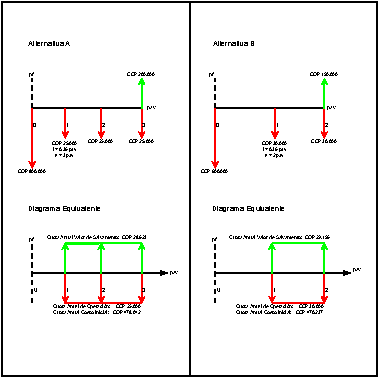
\includegraphics[trim=-5 -5 -5 -5 , scale=2]{10_Capitulo/ejemplos/2/Ejemplo_2.pdf}}
        \\\hline
		%%%%%%%%%%%%% FIN INSERCIÓN DE IMAGEN
		%%%%%FIN FLUJO DE CAJA



		%%%%% INICIO DECLARACIÓN FORMULAS
		%%%%%%%%%%% INICIO TITULO
		\rowcolor[HTML]{FFB183}
		\multicolumn{3}{|c|}{\cellcolor[HTML]{FFB183}\textbf{4. Declaración de fórmulas}} \\ \hline
		%%%%%%%%%%% FIN TITULO
		%%%%%%%%%%% INICIO MATEMÁTICAS

		\multicolumn{3}{|c|}{$VP=R\frac{1-(1+i_{1})^{-n}}{i_{2}} \text{ Valor presente serie uniforme vencida}$}\\ 
		\multicolumn{3}{|c|}{$VF=R\frac{1-(1+i_{1})^{n}}{i_{2}} \text{ Valor futuro aserie uniforme vencida}$}\\\hline
		%%%%%%%%%% FIN MATEMÁTICAS
		%%%%%% INICIO DESARROLLO MATEMÁTICO
		\rowcolor[HTML]{FFB183}
		%%%%%%%%%%INICIO TITULO
		\multicolumn{3}{|c|}{\cellcolor[HTML]{FFB183}\textbf{5. Desarrollo matemático}}   \\ \hline
		%%%%%%%%%% FIN TITULO
		%%%%%%%%%% INICIO MATEMÁTICAS
		Alternativa A & \multicolumn{2}{c|}{Alternativa B}\\ \hline
		Cuota anual costo inicial & \multicolumn{2}{c|}{Cuota anual costo inicial} \\
		${R=\frac{800{.}000}{\frac{1-(1,36)^{-3}}{0,36}} = 178{.}042}\text{ COP}$ & \multicolumn{2}{c|}{${R=\frac{600{.}000}{\frac{1-(1,36)^{-2}}{0,36}} = 470{.}237 }\text{ COP}$} \\
		Cuota anual valor salvamento & \multicolumn{2}{c|}{Cuota anual valor salvamento}\\
		$R=\frac{200{.}000}{\frac{(1,36)^{3}}{0,36}} = 28{.}623\text{ COP} $ & \multicolumn{2}{c|}{$R=\frac{150{.}000}{\frac{(1,36)^{2}}{0,36}} = 29{.}196 \text{ COP}$} \\
		CPUE alternativa A & \multicolumn{2}{c|}{CPUE alternativa B} \\ 
		$CPUE_{A} = 28.623-478.042-25.000 $ & \multicolumn{2}{c|}{$CPUE_{B} = 29.196-470.237-30.000$}\\ 
		$CPUE_{A} = -474.419\text{ COP}$ & \multicolumn{2}{c|}{$CPUE_{B} = -471.04$\text{ COP}}\\
		\hline
		%%%%%%%%%% FIN MATEMÁTICAS
		%%%%%% FIN DESARROLLO MATEMÁTICO

		\rowcolor[HTML]{FFB183}
		\multicolumn{3}{|c|}{\cellcolor[HTML]{FFB183}\textbf{6. Respuesta}}    \\ \hline

		\multicolumn{3}{|c|}{La alternativa que representa menores perdidad es la B.} \\ 
		\hline
	\end{longtable}
	%Se crean dos lineas en blanco para que no quede el siguiente texto tan pegado
	%\newline \newline
\end{center}
%%%%%%%%%%%%%%%%%%%%%%%%%%FIN EJERCICIO X %%%%%%%%%%%%%%%%%%%%%%%%%%%




\section{Tasa de interés nominal anual (j)}
Corresponde a la anualización de la tasa periódica (i):\\
$j = i(m)$\\
%%%%%%%%%% NO OLVIDAR COLOCAR ESTE COMENTARIO CON EL NUMERO DE EJERCICIO %%%%%%%%%%%%%
%%%%%%%%%%%%%%%%%%% EJERCICIO 2 %%%%%%
%%Text bf para negrilla , el \\ es para el salto de linea.
%%El primer \\ hace un espacio en el texto y el 2 \\ crea otro espacio
\textbf{Ejemplo 2}\newline
El jefe de producción de una fábrica debe decidir entre dos máquinas A y B. Las características de cada una son: \\
\begin{center}
		\begin{tabular}{|p{1cm}|p{2cm}|p{2cm}|p{2cm}|p{3cm}|}
			\hline
			\rowcolor{white!50}
			\textbf{Maq.} & \textbf{C} & \textbf{K} & \textbf{S} & \textbf{CAO} \\ \hline
			A            & 800.000 COP   & 3 años     & 200.000 COP    & 25.000 COP       \\ \hline
			B            & 600.000 COP   & 2 años     & 150.000 COP    & 30.000 COP       \\ \hline
		\end{tabular}
\end{center}

Con una tasa del 36\% nominal anual año vencido, determinar la mejor alternativa.

\textbf{Solución.}\\
\begin{center}
	\renewcommand{\arraystretch}{1.5}% Margenes de las celdas
	%Creación de la cuadricula
	\begin{longtable}[H]{|c|c|c|}
		%Creamos una linea horizontal
		\hline
		%Definimos el color de la primera fila
		\rowcolor[HTML]{FFB183}
		%%%%% INICIO ASIGNACIÓN FECHA FOCAL %%%%%%%
		%%%%%%%%%% INICIO TITULO
		%Lo que se hace aquí es mezclar las 3 columnas en una sola
		\multicolumn{3}{|c|}{\cellcolor[HTML]{FFB183}\textbf{1. Asignación período focal}}   \\ \hline
		%%%%%%%%%% FIN TITULO
		%%%%% INICIO DECLARACIÓN DE VARIABLES %%%%%%%
		\multicolumn{3}{|c|}{$pf = 0  \textit{ pav }$} \\ \hline
		%Definimos el color de la primera fila
		\rowcolor[HTML]{FFB183}
		%%%%% INICIO DECLARACIÓN DE VARIABLES %%%%%%%
		%%%%%%%%%% INICIO TITULO
		\multicolumn{3}{|c|}{\cellcolor[HTML]{FFB183}\textbf{2. Declaración de variables}}                                                                                   \\ \hline
		%%%%%%%%%% FIN TITULO
		%%%%%%%%%% INICIO DE MATEMÁTICAS
		$\text{Alternativa A}$ & $\text{Alternativa B}$ & $i= 36\% \text{ pav }$\\
		$C =  800{.}000\text{ COP}$ & $C =  600{.}000\text{ COP}$ & $CPUE =  ?\text{ COP}$\\
		$K =  3 \textit{ años}$ & $K =  2 \textit{ años}$ & \\
		$S =  200{.}000\text{ COP}$ & $S =  150{.}000\text{ COP}$ & \\
		$CAO =  25{.}000\text{ COP}$ & $CAO =  30{.}000\text{ COP}$ & \\
 		$n_{1}= 3 \text{ pav}$ & $n_{2}= 2 \text{ pav}$ &   \\\hline 
		%%%%%%%%%% FIN DE MATEMÁTICAS
		%%%%% FIN DECLARACIÓN DE VARIABLES


		%%%%% INICIO FLUJO DE CAJA
		\rowcolor[HTML]{FFB183}
		\multicolumn{3}{|c|}{\cellcolor[HTML]{FFB183}\textbf{3. Diagrama de flujo de caja}}\\ \hline
		%Mezclamos 3 columnas y pondremos el dibujo
		%%%%%%%%%%%%% INSERCIÓN DE LA IMAGEN
		\multicolumn{3}{|c|}{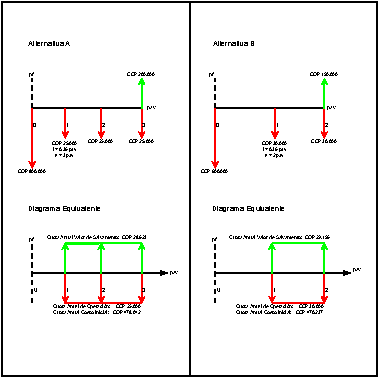
\includegraphics[trim=-5 -5 -5 -5 , scale=2]{10_Capitulo/ejemplos/2/Ejemplo_2.pdf}}
        \\\hline
		%%%%%%%%%%%%% FIN INSERCIÓN DE IMAGEN
		%%%%%FIN FLUJO DE CAJA



		%%%%% INICIO DECLARACIÓN FORMULAS
		%%%%%%%%%%% INICIO TITULO
		\rowcolor[HTML]{FFB183}
		\multicolumn{3}{|c|}{\cellcolor[HTML]{FFB183}\textbf{4. Declaración de fórmulas}} \\ \hline
		%%%%%%%%%%% FIN TITULO
		%%%%%%%%%%% INICIO MATEMÁTICAS

		\multicolumn{3}{|c|}{$VP=R\frac{1-(1+i_{1})^{-n}}{i_{2}} \text{ Valor presente serie uniforme vencida}$}\\ 
		\multicolumn{3}{|c|}{$VF=R\frac{1-(1+i_{1})^{n}}{i_{2}} \text{ Valor futuro aserie uniforme vencida}$}\\\hline
		%%%%%%%%%% FIN MATEMÁTICAS
		%%%%%% INICIO DESARROLLO MATEMÁTICO
		\rowcolor[HTML]{FFB183}
		%%%%%%%%%%INICIO TITULO
		\multicolumn{3}{|c|}{\cellcolor[HTML]{FFB183}\textbf{5. Desarrollo matemático}}   \\ \hline
		%%%%%%%%%% FIN TITULO
		%%%%%%%%%% INICIO MATEMÁTICAS
		Alternativa A & \multicolumn{2}{c|}{Alternativa B}\\ \hline
		Cuota anual costo inicial & \multicolumn{2}{c|}{Cuota anual costo inicial} \\
		${R=\frac{800{.}000}{\frac{1-(1,36)^{-3}}{0,36}} = 178{.}042}\text{ COP}$ & \multicolumn{2}{c|}{${R=\frac{600{.}000}{\frac{1-(1,36)^{-2}}{0,36}} = 470{.}237 }\text{ COP}$} \\
		Cuota anual valor salvamento & \multicolumn{2}{c|}{Cuota anual valor salvamento}\\
		$R=\frac{200{.}000}{\frac{(1,36)^{3}}{0,36}} = 28{.}623\text{ COP} $ & \multicolumn{2}{c|}{$R=\frac{150{.}000}{\frac{(1,36)^{2}}{0,36}} = 29{.}196 \text{ COP}$} \\
		CPUE alternativa A & \multicolumn{2}{c|}{CPUE alternativa B} \\ 
		$CPUE_{A} = 28.623-478.042-25.000 $ & \multicolumn{2}{c|}{$CPUE_{B} = 29.196-470.237-30.000$}\\ 
		$CPUE_{A} = -474.419\text{ COP}$ & \multicolumn{2}{c|}{$CPUE_{B} = -471.04$\text{ COP}}\\
		\hline
		%%%%%%%%%% FIN MATEMÁTICAS
		%%%%%% FIN DESARROLLO MATEMÁTICO

		\rowcolor[HTML]{FFB183}
		\multicolumn{3}{|c|}{\cellcolor[HTML]{FFB183}\textbf{6. Respuesta}}    \\ \hline

		\multicolumn{3}{|c|}{La alternativa que representa menores perdidad es la B.} \\ 
		\hline
	\end{longtable}
	%Se crean dos lineas en blanco para que no quede el siguiente texto tan pegado
	%\newline \newline
\end{center}
%%%%%%%%%%%%%%%%%%%%%%%%%%FIN EJERCICIO X %%%%%%%%%%%%%%%%%%%%%%%%%%%



\textbf{Ejemplo 3}\\
Hallar el valor presente de la siguiente serie con una tasa del 5\% periodo anual mes vencido, utilizando dos formas para resolverlo.\\

%imagen 4
\begin{center}
	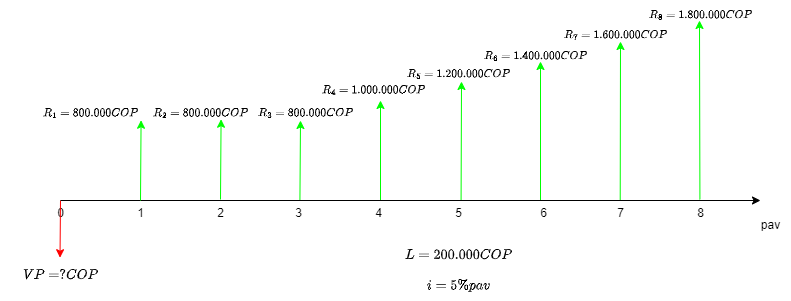
\includegraphics[height=4.0cm]{6_Capitulo/img/ejemplos/6_5}
\end{center}

\textbf{Solución:}

\begin{center}
	\textbf{Primera forma:}
\end{center}

%La tabla ira centrada
\begin{center}
	\renewcommand{\arraystretch}{1.4}% Margenes de las celdas
	%Creación de la cuadricula de 3 columnas
	\begin{longtable}[H]{|c|c|c|}
		%Creamos una linea horizontal
		\hline
		%Definimos el color de la primera fila
		\rowcolor[HTML]{FFB183}
		%%%%% INICIO ASIGNACIÓN PERIODO FOCAL %%%%%%%
		%%%%%%%%%% INICIO TITULO
		%Lo que se hace aquí es mezclar las 3 columnas en una sola
		\multicolumn{3}{|c|}{\cellcolor[HTML]{FFB183}\textbf{1. Asignación período focal}}                                                                                                                            \\ \hline
		\multicolumn{3}{|c|}{$Pf=0 \textit{ pav}$}                                                                                                                                                                    \\ \hline
		%%%%%%%%%% FIN TITULO
		%%%%% INICIO DECLARACIÓN DE VARIABLES %%%%%%%
		%%%%%%%%%% INICIO TITULO
		%Lo que se hace aquí es mezclar las 3 columnas en una sola
		\multicolumn{3}{|c|}{\cellcolor[HTML]{FFB183}\textbf{2. Declaración de variables}}                                                                                                                            \\ \hline
		%%%%%%%%%% FIN TITULO
		%%%%%%%%%% INICIO DE MATEMÁTICAS
		%Cada & hace referencia al paso de la siguiente columna
		\multicolumn{2}{|c|}{$\hspace{2 cm}R=800{.}000 COP \hspace{2 cm}$} & $i=5\%\textit{ pav}$                                                                                                                     \\
		\multicolumn{2}{|c|}{$L=  200{.}000COP$}                           & $n_1=2\textit{ pav}$                                                                                                                     \\
		\multicolumn{2}{|c|}{$VP= ?COP $}                                  & $n_2=6\textit{ pav}$                                                                                                                     \\\hline

		%%%%%%%%%% FIN DE MATEMÁTICAS
		%%%%% FIN DECLARACIÓN DE VARIABLES


		%%%%% INICIO FLUJO DE CAJA
		\rowcolor[HTML]{FFB183}
		\multicolumn{3}{|c|}{\cellcolor[HTML]{FFB183}\textbf{3. Diagrama de flujo de caja}}                                                                                                                           \\ \hline
		%Mezclamos 3 columnas y pondremos el dibujo
		%%%%%%%%%%%%% INSERCIÓN DE LA IMAGEN
		%Deberán descargar las imágenes respectivas del drive y pegarlas en la carpeta
		%n_capitulo/img/ejemplos/1/capitulo1ejemplo1.pdf  (el /1/ es el numero del ejemplo)
		\multicolumn{3}{|c|}{ 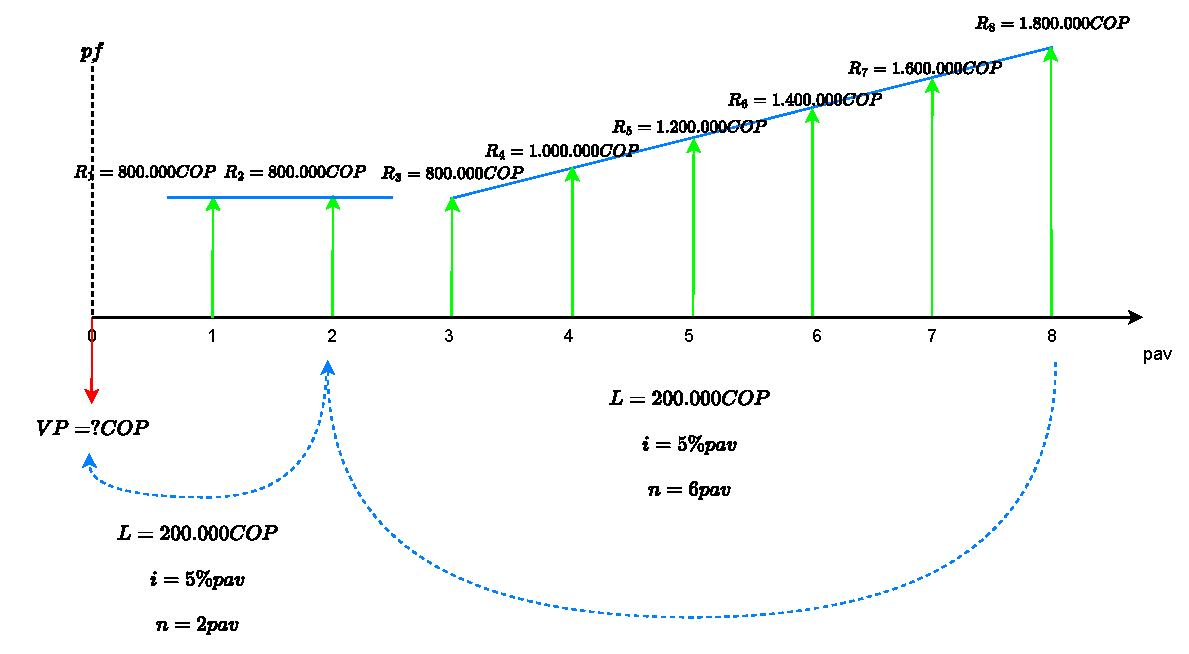
\includegraphics[trim=-5 -5 -5 -5 , scale=0.4]{6_Capitulo/ejemplos/3/Capitulo6Ejemplo3a.pdf} }

		\\ \hline
		%%%%%%%%%%%%% FIN INSERCIÓN DE IMAGEN
		%%%%%FIN FLUJO DE CAJA

		%%%%% INICIO DECLARACIÓN FORMULAS
		%%%%%%%%%%% INICIO TITULO
		\rowcolor[HTML]{FFB183}
		\multicolumn{3}{|c|}{\cellcolor[HTML]{FFB183}\textbf{4. Declaración de fórmulas}}                                                                                                                             \\ \hline
		%%%%%%%%%%% FIN TITULO
		%%%%%%%%%%% INICIO MATEMÁTICAS

		\multicolumn{3}{|c|}{$VP=R(\frac{1-(1+i)^{-n}}{i})+\frac{L}{i}[\frac{1-(1+i)^{-n}}{i}-n(1+i)^{-n}] \hspace{0.4 cm} \textit{Valor presente gradiente aritmético}$}                                             \\
		\multicolumn{3}{|c|}{$VP=R(\frac{1-(1+i)^{-n}}{i}) \hspace{0.4 cm} \textit{Valor presente de una serie unifrome vencida}$}                                                                                    \\
		\multicolumn{3}{|c|}{$P=F(1+i)^{-n} \hspace{0.4 cm} \textit{Valor presente dado un valor futuro}$}                                                                                                            \\ \hline

		%%%%%%%%%% FIN MATEMÁTICAS
		%%%%%% INICIO DESARROLLO MATEMÁTICO
		\rowcolor[HTML]{FFB183}
		%%%%%%%%%%INICIO TITULO
		\multicolumn{3}{|c|}{\cellcolor[HTML]{FFB183}\textbf{5. Desarrollo matemático}}                                                                                                                               \\ \hline
		%%%%%%%%%% FIN TITULO
		%%%%%%%%%% INICIO MATEMÁTICAS
		\multicolumn{3}{|c|}{$VP=  800{.}000COP(\frac{1-(1+0.05)^{-2}}{0.05})+[  800{.}000COP(\frac{1-(1+0.05)^{-6}}{0.05})+\frac{ COP 200{.}000}{0.05}[\frac{1-(1+0.05)^{-6}}{0.05}-6(1+0.05)^{-6}]]$} \\
		\multicolumn{3}{|c|}{$*(1+0.05)^{-2}$}\\
		\multicolumn{3}{|c|}{$VP= 7{.}341{.} \textit{  COP }$}                                                                                                                                                       \\ \hline


		%%%%%%%%%% FIN MATEMÁTICAS
		%%%%%% FIN DESARROLLO MATEMÁTICO
		%%%%%% INICIO RESPUESTA
		\rowcolor[HTML]{FFB183}
		%%%%%%%%%%INICIO TITULO
		\multicolumn{3}{|c|}{\cellcolor[HTML]{FFB183}\textbf{6. Respuesta}}                                                                                                                                           \\ \hline
		%%%%%%%%%% FIN TITULO
		%%%%%%%%%% INICIO RESPUESTA MATEMÁTICA
		\multicolumn{3}{|c|}{\textbf{$\textit{VP= 7{.}341{.}634.83  COP }$}}
		\\ \hline
		%%%%%%%%%% FIN MATEMÁTICAS
		%%%%%% FIN RESPUESTA
	\end{longtable}
	%Se crean dos lineas en blanco para que no quede el siguiente texto tan pegado
	%\newline \newline %USARLO SI CREES QUE ES NECESARIO
\end{center}
%%%%%%%%%%%%%%%%%%%%%%%%%%FIN EJERCICIO 3.1 %%%%%%%%%%%%%%%%%%%%%%%%%%%

\textbf{Segunda forma:}


%La tabla ira centrada
\begin{center}
	\renewcommand{\arraystretch}{1.4}% Margenes de las celdas
	%Creación de la cuadricula de 3 columnas
	\begin{longtable}[H]{|c|c|c|}
		%Creamos una linea horizontal
		\hline
		%Definimos el color de la primera fila
		\rowcolor[HTML]{FFB183}
		%%%%% INICIO ASIGNACIÓN PERIODO FOCAL %%%%%%%
		%%%%%%%%%% INICIO TITULO
		%Lo que se hace aquí es mezclar las 3 columnas en una sola
		\multicolumn{3}{|c|}{\cellcolor[HTML]{FFB183}\textbf{1. Asignación período focal}}                                                                                                                                                            \\ \hline
		\multicolumn{3}{|c|}{$pf=0 \textit{ pav}$}                                                                                                                                                                                                    \\ \hline
		%%%%%%%%%% FIN TITULO
		%%%%% INICIO DECLARACIÓN DE VARIABLES %%%%%%%
		%%%%%%%%%% INICIO TITULO
		%Lo que se hace aquí es mezclar las 3 columnas en una sola
		\multicolumn{3}{|c|}{\cellcolor[HTML]{FFB183}\textbf{2. Declaración de variables}}                                                                                                                                                            \\ \hline
		%%%%%%%%%% FIN TITULO
		%%%%%%%%%% INICIO DE MATEMÁTICAS
		%Cada & hace referencia al paso de la siguiente columna
		\multicolumn{2}{|c|}{$\hspace{2 cm}R=  800{.}000COP\hspace{2 cm}$} & $i=5\%\textit{ pav}$                                                                                                                                                     \\
		\multicolumn{2}{|c|}{$L=  200{.}000COP$}                           & $n_1=3\textit{ pav}$                                                                                                                                                     \\
		\multicolumn{2}{|c|}{$VP=? COP $}                                  & $n_2=5\textit{ pav}$                                                                                                                                                     \\\hline

		%%%%%%%%%% FIN DE MATEMÁTICAS
		%%%%% FIN DECLARACIÓN DE VARIABLES


		%%%%% INICIO FLUJO DE CAJA
		\rowcolor[HTML]{FFB183}
		\multicolumn{3}{|c|}{\cellcolor[HTML]{FFB183}\textbf{3. Diagrama de flujo de caja}}                                                                                                                                                           \\ \hline
		%Mezclamos 3 columnas y pondremos el dibujo
		%%%%%%%%%%%%% INSERCIÓN DE LA IMAGEN
		%Deberán descargar las imágenes respectivas del drive y pegarlas en la carpeta
		%n_capitulo/img/ejemplos/1/capitulo1ejemplo1.pdf  (el /1/ es el numero del ejemplo)
		\multicolumn{3}{|c|}{ 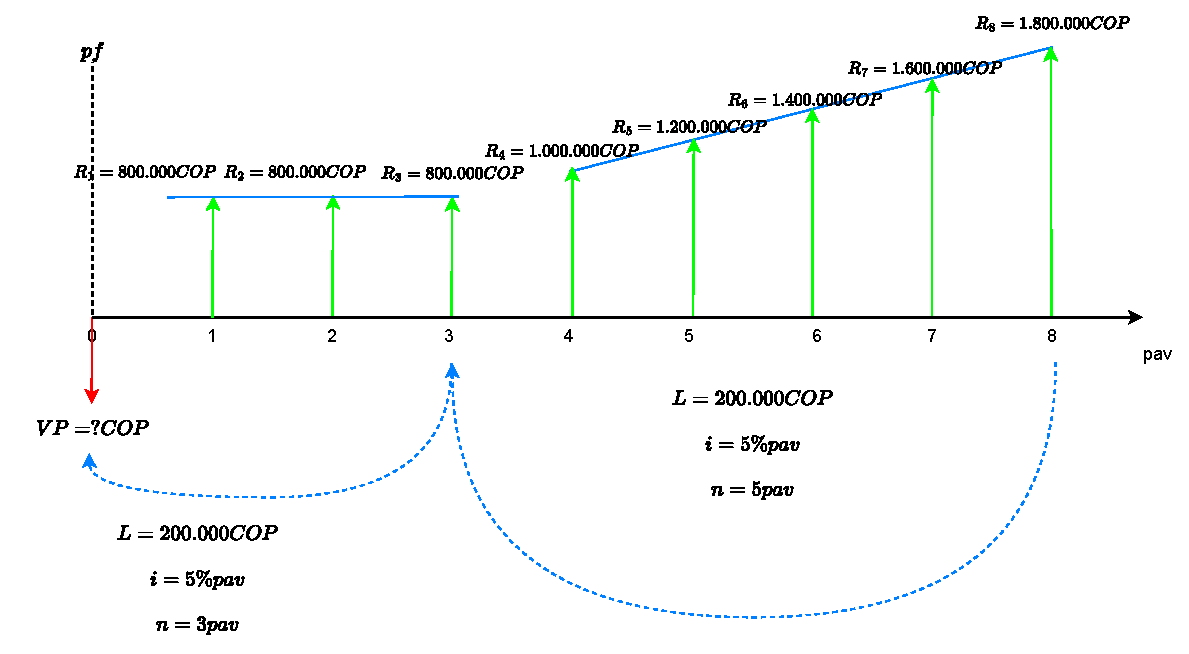
\includegraphics[trim=-5 -5 -5 -5 , scale=0.4]{6_Capitulo/ejemplos/3/Capitulo6Ejemplo3b.pdf} }

		\\ \hline
		%%%%%%%%%%%%% FIN INSERCIÓN DE IMAGEN
		%%%%%FIN FLUJO DE CAJA

		%%%%% INICIO DECLARACIÓN FORMULAS
		%%%%%%%%%%% INICIO TITULO
		\rowcolor[HTML]{FFB183}
		\multicolumn{3}{|c|}{\cellcolor[HTML]{FFB183}\textbf{4. Declaración de fórmulas}}                                                                                                                                                             \\ \hline
		%%%%%%%%%%% FIN TITULO
		%%%%%%%%%%% INICIO MATEMÁTICAS

		\multicolumn{3}{|c|}{$VP=R(\frac{1-(1+i)^{-n}}{i})+\frac{L}{i}[\frac{1-(1+i)^{-n}}{i}-n(1+i)^{-n}] \hspace{0.4 cm} \textit{Valor presente gradiente aritmético}$}                                                                             \\
		\multicolumn{3}{|c|}{$VP=R(\frac{1-(1+i)^{-n}}{i}) \hspace{0.4 cm} \textit{Valor presente de una serie unifrome vencida}$}                                                                                                                    \\
		\multicolumn{3}{|c|}{$P=F(1+i)^{-n} \hspace{0.4 cm} \textit{Valor presente dado un valor futuro}$}                                                                                                                                            \\ \hline

		%%%%%%%%%% FIN MATEMÁTICAS
		%%%%%% INICIO DESARROLLO MATEMÁTICO
		\rowcolor[HTML]{FFB183}
		%%%%%%%%%%INICIO TITULO
		\multicolumn{3}{|c|}{\cellcolor[HTML]{FFB183}\textbf{5. Desarrollo matemático}}                                                                                                                                                               \\ \hline
		%%%%%%%%%% FIN TITULO
		%%%%%%%%%% INICIO MATEMÁTICAS
		\multicolumn{3}{|c|}{$VP=  800{.}000COP(\frac{1-(1+0.05)^{-3}}{0.05})+[  1{.}000{.}000COP(\frac{1-(1+0.05)^{-5}}{0.05})+\frac{  200{.}000COP}{0.05}[\frac{1-(1+0.05)^{-5}}{0.05}-6(1+0.05)^{-6}]]$} \\
		\multicolumn{3}{|c|}{$*(1+0.05)^{-3}\hspace{0.2 cm}\textit{Ec. eqv.}$}\\
		\multicolumn{3}{|c|}{$VP= 7{.}341{.}634 \textit{  COP }$}                                                                                                                                                                                       \\ \hline


		%%%%%%%%%% FIN MATEMÁTICAS
		%%%%%% FIN DESARROLLO MATEMÁTICO
		%%%%%% INICIO RESPUESTA
		\rowcolor[HTML]{FFB183}
		%%%%%%%%%%INICIO TITULO
		\multicolumn{3}{|c|}{\cellcolor[HTML]{FFB183}\textbf{6. Respuesta}}                                                                                                                                                                           \\ \hline
		%%%%%%%%%% FIN TITULO
		%%%%%%%%%% INICIO RESPUESTA MATEMÁTICA
		\multicolumn{3}{|c|}{{$\textit{El valor presente de la serie es  7{.}341{.}634 COP }$}}
		\\ \hline
		%%%%%%%%%% FIN MATEMÁTICAS
		%%%%%% FIN RESPUESTA
	\end{longtable}
	%Se crean dos lineas en blanco para que no quede el siguiente texto tan pegado
	%\newline \newline %USARLO SI CREES QUE ES NECESARIO
\end{center}
%%%%%%%%%%%%%%%%%%%%%%%%%%FIN EJERCICIO 3.2 %%%%%%%%%%%%%%%%%%%%%%%%%%%



\section{Equivalencia de tasas ($i_{1} \equiv i_{2}$)}
Las tasas equivalentes de interés,  son aquellas que teniendo diferente periodicidad y/o 
modalidad de liquidación de intereses producen el mismo monto al final o al comienzo del flujo.\\
\\
\textbf{Ejemplo 4}\\
	Hallar el monto del siguiente flujo de caja que renta una tasa del 15\% periódica año vencido. \\
	\\
	%imagen 5
	\begin{center}
		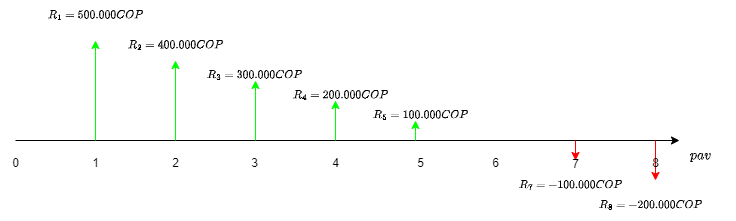
\includegraphics[height=4.5cm]{6_Capitulo/img/ejemplos/6_6}
	\end{center}
	
	\textbf{Solución:}
	
		%La tabla ira centrada
	\begin{center}
		\renewcommand{\arraystretch}{1.4}% Margenes de las celdas
		%Creación de la cuadricula de 3 columnas
		\begin{longtable}[H]{|c|c|c|}
			%Creamos una linea horizontal
			\hline
			%Definimos el color de la primera fila
			\rowcolor[HTML]{FFB183}
			%%%%% INICIO ASIGNACIÓN PERIODO FOCAL %%%%%%%
			%%%%%%%%%% INICIO TITULO
			%Lo que se hace aquí es mezclar las 3 columnas en una sola
			\multicolumn{3}{|c|}{\cellcolor[HTML]{FFB183}\textbf{1. Asignación período focal}}  \\ \hline
			\multicolumn{3}{|c|}{$pf=8 \textit{ pav}$} \\ \hline
			%%%%%%%%%% FIN TITULO
			%%%%% INICIO DECLARACIÓN DE VARIABLES %%%%%%%
			%%%%%%%%%% INICIO TITULO
			%Lo que se hace aquí es mezclar las 3 columnas en una sola
			\multicolumn{3}{|c|}{\cellcolor[HTML]{FFB183}\textbf{2. Declaración de variables}}   \\ \hline
			%%%%%%%%%% FIN TITULO
			%%%%%%%%%% INICIO DE MATEMÁTICAS
			%Cada & hace referencia al paso de la siguiente columna
			\multicolumn{2}{|c|}{$\hspace{2 cm}R=  500{.}000COP\hspace{2 cm}$} & $i=15\%\textit{ pav}$ \\
			\multicolumn{2}{|c|}{$L=-  100{.}000COP$} & $n_1=8\textit{ pav}$ \\ 
			\multicolumn{2}{|c|}{$VF= ?COP $} &  \\\hline
			
			%%%%%%%%%% FIN DE MATEMÁTICAS
			%%%%% FIN DECLARACIÓN DE VARIABLES
			
			
			%%%%% INICIO FLUJO DE CAJA
			\rowcolor[HTML]{FFB183}
			\multicolumn{3}{|c|}{\cellcolor[HTML]{FFB183}\textbf{3. Diagrama de flujo de caja}} \\ \hline
			%Mezclamos 3 columnas y pondremos el dibujo
			%%%%%%%%%%%%% INSERCIÓN DE LA IMAGEN
			%Deberán descargar las imágenes respectivas del drive y pegarlas en la carpeta
			%n_capitulo/img/ejemplos/1/capitulo1ejemplo1.pdf  (el /1/ es el numero del ejemplo)
			\multicolumn{3}{|c|}{ 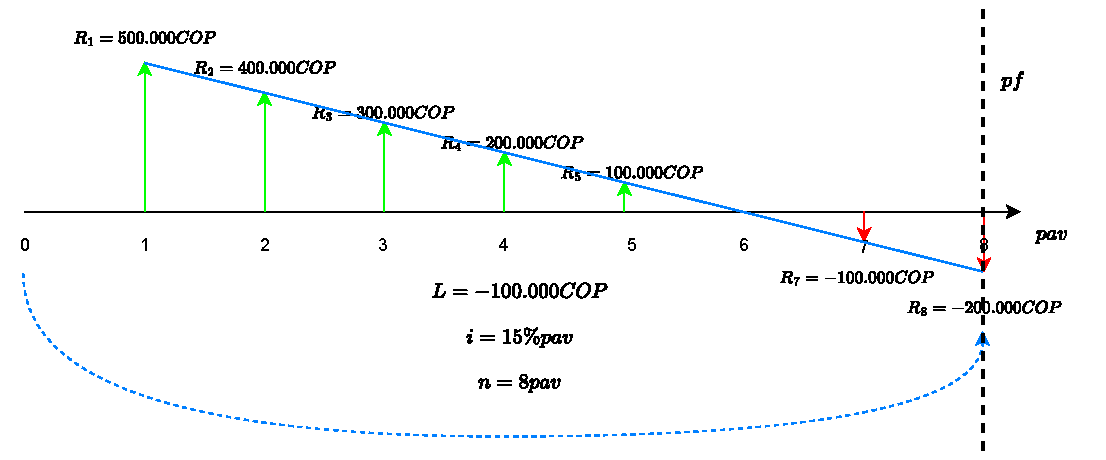
\includegraphics[trim=-5 -5 -5 -5 , scale=0.4]{6_Capitulo/ejemplos/4/Capitulo6Ejemplo4.pdf} }
			
			\\ \hline
			%%%%%%%%%%%%% FIN INSERCIÓN DE IMAGEN
			%%%%%FIN FLUJO DE CAJA
			
			%%%%% INICIO DECLARACIÓN FORMULAS
			%%%%%%%%%%% INICIO TITULO
			\rowcolor[HTML]{FFB183}
			\multicolumn{3}{|c|}{\cellcolor[HTML]{FFB183}\textbf{4. Declaración de fórmulas}}    \\ \hline
			%%%%%%%%%%% FIN TITULO
			%%%%%%%%%%% INICIO MATEMÁTICAS
			
			\multicolumn{3}{|c|}{$VF=R(\frac{(1+i)^{n}-1}{i})+\frac{L}{i}[\frac{(1+i)^{n}-1}{i}-n] \hspace{0.4 cm} \textit{Valor final de gradiente aritmético}$} \\ \hline
			
			%%%%%%%%%% FIN MATEMÁTICAS
			%%%%%% INICIO DESARROLLO MATEMÁTICO
			\rowcolor[HTML]{FFB183}
			%%%%%%%%%%INICIO TITULO
			\multicolumn{3}{|c|}{\cellcolor[HTML]{FFB183}\textbf{5. Desarrollo matemático}}       \\ \hline
			%%%%%%%%%% FIN TITULO
			%%%%%%%%%% INICIO MATEMÁTICAS
			\multicolumn{3}{|c|}{$VF=  500{.}000COP(\frac{(1+0.15)^{8}-1}{0.15})+\frac{-  100{.}000COP}{0.15}[\frac{(1+0.15)^{8}-1}{0.15}-8]\hspace{0.4 cm}\textit{Ecuación de equivalencia}$} \\
			\multicolumn{3}{|c|}{$VF=  3{.}045{.}000 \textit{  COP }$} \\ \hline
			
			
			%%%%%%%%%% FIN MATEMÁTICAS
			%%%%%% FIN DESARROLLO MATEMÁTICO
			%%%%%% INICIO RESPUESTA
			\rowcolor[HTML]{FFB183}
			%%%%%%%%%%INICIO TITULO
			\multicolumn{3}{|c|}{\cellcolor[HTML]{FFB183}\textbf{6. Respuesta}}   \\ \hline
			%%%%%%%%%% FIN TITULO
			%%%%%%%%%% INICIO RESPUESTA MATEMÁTICA
			\multicolumn{3}{|c|}{{$\textit{El monto o valor final del flujo de caja es  3{.}045.000  COP }$}}
			\\ \hline
			%%%%%%%%%% FIN MATEMÁTICAS
			%%%%%% FIN RESPUESTA
		\end{longtable}
		%Se crean dos lineas en blanco para que no quede el siguiente texto tan pegado
		%\newline \newline %USARLO SI CREES QUE ES NECESARIO
	\end{center}
	%%%%%%%%%%%%%%%%%%%%%%%%%%FIN EJERCICIO 4 %%%%%%%%%%%%%%%%%%%%%%%%%%%


\section{Relación entre una tasa de interés anticipada(i$_{a}$) y una tasa vencida(i)}
Para $n = 1$, se tiene
$i = \frac{I}{P}$ \\
Si $I = F  d \land P = F (1 -d)$ \hspace{35 pt}\textit{Tasa nominal anual}\\\\
Remplazando en i: \\
$i = \frac {F d} {F (1-d)}$\\\\
Factorizando F,  se obtiene: \\
$i = \frac{d}{(1 - d)}$\\
Remplazando $d = i_{a} $, se obtiene: \\
$i = \frac{ia}{(1 - ia)}$\\\\
Despejando $i_{a}$: \\
$i_{a} = \frac{i}{(1+i)}$ \\\\
$i = \frac{I}{P} = \frac{F d}{F(1-d)}$\\\\
$i = \frac{d}{1-d}$\\

Reemplazando d = $i_{a}$, se obtiene:\\

$i_{a} = \frac{i}{1+i}$\hspace{35 pt}\textit{Tasa periódica anticipada}\\
$j_{a} = i_{a}  (m)$\hspace{23 pt}\textit{Tasa nominal anual anticipada}\\\\

\section{Tasa de interés nominal anual (j) y tasa efectiva anual (EA)}
Según la Superintendencia Financiera de Colombia, la tasa de interés nominal anual es la tasa que el emisor paga al inversionista por un título valor.
Las tasas nominales anuales corresponden a la anualización de una tasa \textbf{periódica}. \\
De igual forma, pueden tener modalidad vencida o anticipada para la liquidación de intereses.\\

\textbf{Tasa de interés efectiva anual (EA):} La tasa de interés efectiva anual, es el instrumento apropiado para medir y comparar, el rendimiento de distintas alternativas de inversión según la Superintendencia Financiera.\\
Según el profesor Javier Serrano, en el libro “Matemáticas financieras y evaluación de proyectos”, la tasa de interés efectiva anual (EA) corresponde a aquella tasa que paga de una sola vez al final del año.\\

Para calcular la tasa efectiva anual, se parte de la fórmula de equivalencia de tasas en donde el
período es anual vencido.

$(1 + i_1)^{m_1} = (1 + i_2)^{m_2}$ , en donde $i_1$ = tasa periódica, que anualizada ($j_1$) es equivalente a la tasa efectiva anual, para un $m_1 = 1 pav$.\\

IMPORTANTE: La tasa Efectiva Anual es equivalente a la tasa Nominal Anual Año Vencido. (naav) \\


\section{Gráfica de equivalencia de tasas}
Gráfica idónea para realizar una equivalencia entre tasas, utilizando las ecuaciones previamente analizadas, se verá que podemos partir de una tasa cualquiera e ir a otra sin necesidad de información adicional.\\
Los puntos que se han colocado del 1 al 8 solo sirven de identificación.\\
\begin{center}
   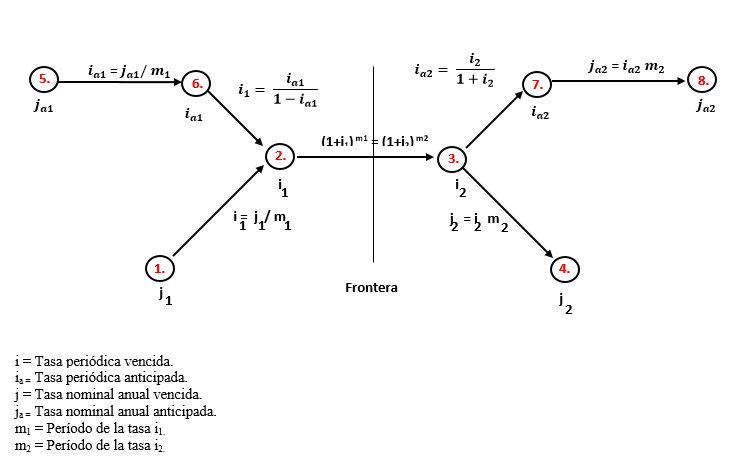
\includegraphics[height = 9.0 cm]{general.png}\\
\end{center}

\textbf{Observación:} Para el uso de la gráfica de equivalencia de tasas, siempre se debe comenzar de un punto de la izquierda y seguir la trayectoria hasta llegar a otro punto situado en la parte derecha.\\
\newpage

\textbf{Ejemplo 5}\\
Hallar el monto, el valor futuro y el valor presente de 20 pagos de 200.000 COP cada uno, suponga una tasa del 24\% nominal anual año vencido.\\ \\
%\newpage %USAR SOLO SI EL SOLUCIÓN QUEDA SOLO Y ES NECESARIO BAJARLO A LA SIGUIENTE PAGINA
\textbf{Solución.}
%La tabla ira centrada
\begin{center}
 \renewcommand{\arraystretch}{1.5}% Margenes de las celdas
 %Creación de la cuadricula de 3 columnas
 \begin{longtable}[H]{|p{0.333\linewidth}|p{0.3333\linewidth}|p{0.3333\linewidth}|}
  \hline
  \multicolumn{3}{|c|}{\cellcolor[HTML]{FFB183}\textbf{1. Declaración de variables}}                   \\ \hline
  $R= 200.000 COP$         & $i=24\% \hspace{1mm} pav$ & $VP = ? COP$                                  \\
  $n=20 \hspace{1mm} pav$ &                            & $VF= ? COP$                                   \\ \hline
  \multicolumn{3}{|c|}{\cellcolor[HTML]{FFB183}\textbf{2. Tabla de flujo de caja}}                     \\ \hline
  \multicolumn{3}{|p{\columnwidth}|}{
  \begin{center}
   \begin{tabular}{ |p{3.5cm}| p{3cm}|}
    \hline

    \textbf{Periodo (psv) } & \textbf{Flujo} \\ \hline
    0                       & -              \\\hline
    1                       &  200.000 COP     \\ \hline
    2                       &  200.000 COP     \\ \hline
    3                       &  200.000 COP     \\ \hline
    4                       &  200.000 COP     \\ \hline
    5                       &  200.000 COP     \\ \hline
    6                       &  200.000 COP     \\ \hline
    7                       &  200.000 COP     \\ \hline
    8                       &  200.000 COP     \\ \hline
    9                       &  200.000 COP     \\ \hline
    10                      &  200.000 COP     \\ \hline
    11                      &  200.000 COP     \\ \hline
    12                      &  200.000 COP     \\ \hline
    13                      &  200.000 COP     \\ \hline
    14                      &  200.000 COP     \\ \hline
    15                      &  200.000 COP     \\ \hline
    16                      &  200.000 COP     \\ \hline
    17                      &  200.000 COP     \\ \hline
    18                      &  200.000 COP     \\ \hline
    19                      &  200.000 COP     \\ \hline
    20                      &  200.000 COP     \\ \hline
   \end{tabular}

  \end{center}
  }                                                                                                   \\ \hline
  \multicolumn{3}{|c|}{\cellcolor[HTML]{FFB183}\textbf{3. Fórmulas utilizadas}}                       \\ \hline
  \multicolumn{3}{|p{\columnwidth}|}{Mediante el uso de Excel:
  \begin{itemize}
   \item VA (Valor actual): Devuelve el valor presente para una inversión
   \item VF (Valor Futuro): Devuelve el valor futuro de una inversión basado en pagos
         periódicos y constantes, y una tasa de interés constante
  \end{itemize}
  }                                                                                                   \\ \hline
  \multicolumn{3}{|c|}{\cellcolor[HTML]{FFB183}\textbf{4. Desarrollo en Excel}}                       \\ \hline
  \multicolumn{3}{|l|}{Se aplicarán las funciones VA y VF de la siguiente forma:}                     \\
  \multicolumn{3}{|c|}{ 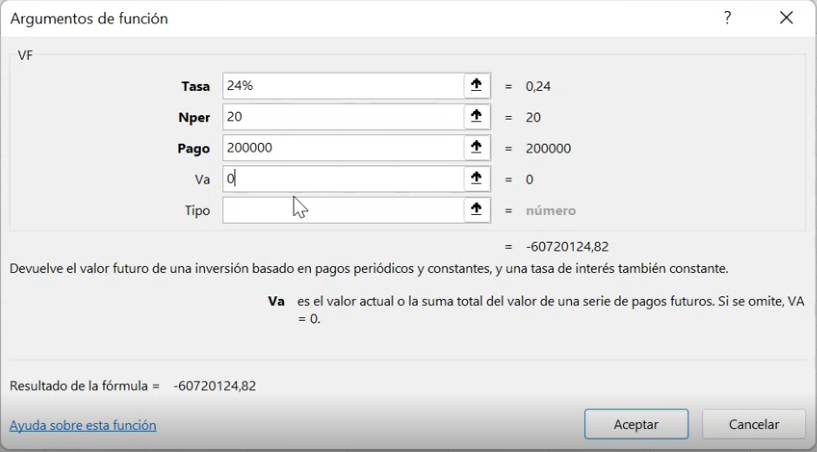
\includegraphics[trim=-5 -5 -5 -5 ,width=1\columnwidth]{5/Ejem5.1.PNG}}        \\
  \multicolumn{3}{|l|}{=VF(0,24;20;-200000;0) con referencia en la hoja de Excel usada para el ejercicio.}    \\
  \multicolumn{3}{|c|}{ 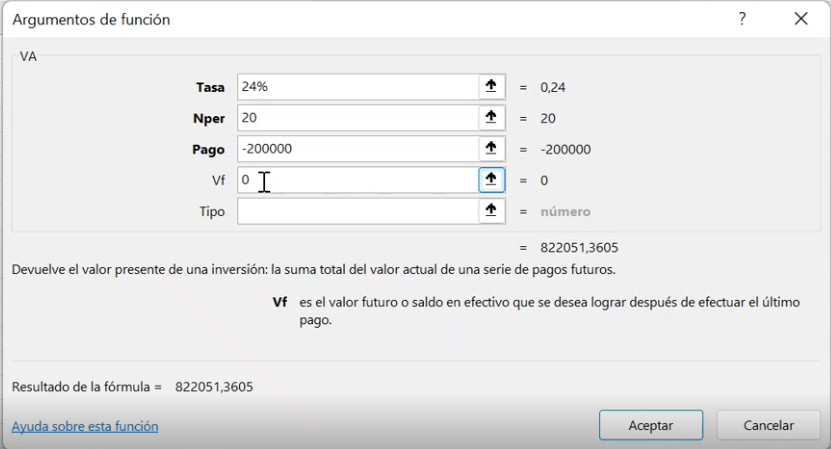
\includegraphics[trim=-5 -5 -5 -5 ,width=1\columnwidth]{5/Ejem5.2.PNG}}        \\
  \multicolumn{3}{|l|}{=VA(0,24;20;-200000;0) con referencia en la hoja de Excel usada para el ejercicio.} \\ \hline
  \multicolumn{3}{|c|}{\cellcolor[HTML]{FFB183}\textbf{5. Respuesta}}                                 \\ \hline
  \multicolumn{3}{|p{\columnwidth}|}{
  El valor presente (VP) o valor actual (VA) es 822.051 COP y el valor futuro (VF) es 60.720.114 COP 
  }                                                                                                   \\ \hline
  \multicolumn{3}{|c|}{\cellcolor[HTML]{FFB183}\textbf{6. Gráfica}}                                   \\ \hline
  \multicolumn{3}{|c|}{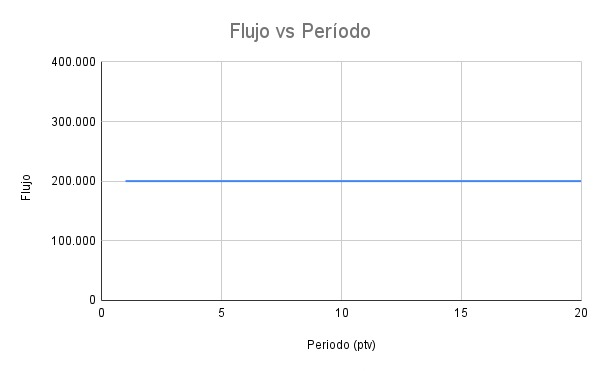
\includegraphics[trim=-5 -5 -5 -5 ,width=0.7\columnwidth]{4/flujovsperiodo.png}}      \\ \hline
 \end{longtable}
 %\newline \newline %USARLO SI CREES QUE ES NECESARIO
\end{center}

	
	\textbf{Ejemplo 6}\\
	Calcular el valor presente de una serie infinita de egresos que crecen en  10{.}000COP, si el primer egreso es de  200{.}000COP y la tasa es del 3\% periódica mes vencido.\\
	
	\newpage
	
	%%%%%%%%%%%%%%%%%%% EJERCICIO 6 %%%%%%
	
	%\newpage %USAR SOLO SI EL SOLUCIÓN QUEDA SOLO Y ES NECESARIO BAJARLO A LA SIGUIENTE PAGINA
	\textbf{Solución.}\\
	%La tabla ira centrada
	\begin{center}
		\renewcommand{\arraystretch}{1.6}% Margenes de las celdas
		%Creación de la cuadricula de 3 columnas
		\begin{longtable}[H]{|c|c|c|}
			%Creamos una linea horizontal
			\hline
			%Definimos el color de la primera fila
			\rowcolor[HTML]{FFB183}
			%%%%% INICIO ASIGNACIÓN FECHA FOCAL %%%%%%%
			%%%%%%%%%% INICIO TITULO
			%Lo que se hace aquí es mezclar las 3 columnas en una sola
			\multicolumn{3}{|c|}{\cellcolor[HTML]{FFB183}\textbf{1. Asignación período focal}}  \\ \hline
			\multicolumn{3}{|c|}{$pf = \textit{0 pmv}$}   \\\hline
			%%%%%%%%%% FIN TITULO
			%%%%% INICIO DECLARACIÓN DE VARIABLES %%%%%%%
			%%%%%%%%%% INICIO TITULO
			%Lo que se hace aquí es mezclar las 3 columnas en una sola
			\multicolumn{3}{|c|}{\cellcolor[HTML]{FFB183}\textbf{2. Declaración de variables}}   \\ \hline
			%%%%%%%%%% FIN TITULO
			%%%%%%%%%% INICIO DE MATEMÁTICAS
			%Cada & hace referencia al paso de la siguiente columna
			\multicolumn{2}{|c|}{\textbf{$\hspace{3.5 cm}\textit{}\hspace{3.5 cm}$}} & \textbf{$\hspace{3.5 cm}\textit{}\hspace{3.5 cm}$} \\ 
			\multicolumn{2}{|c|}{$\hspace{2 cm}L=  10{.}000COP \hspace{2 cm}$} & {$i=3\% \textit{ pmv}$} \\
			\multicolumn{2}{|c|}{$\hspace{2 cm}R=   200{.}000COP \hspace{2 cm}$} & $n=\infty \textit{ pmv}$ \\ 	
			\multicolumn{2}{|c|}{$\hspace{2cm} VP = ? COP \hspace{2 cm}$ } & $$\\ \hline
			%%%%%%%%%% FIN DE MATEMÁTICAS
			%%%%% FIN DECLARACIÓN DE VARIABLES
			
			%%%%% INICIO FLUJO DE CAJA
			\rowcolor[HTML]{FFB183}
			\multicolumn{3}{|c|}{\cellcolor[HTML]{FFB183}\textbf{3. Diagrama de flujo de caja}} \\ \hline
			%Mezclamos 3 columnas y pondremos el dibujo
			%%%%%%%%%%%%% INSERCIÓN DE LA IMAGEN
			%Deberán descargar las imágenes respectivas del drive y pegarlas en la carpeta
			%n_capitulo/img/ejemplos/1/capitulo1ejemplo1.pdf  (el /1/ es el numero del ejemplo)
			\multicolumn{3}{|c|}{ \includegraphics[trim=-5 -5 -5 -5 , scale=0.6]{6_Capitulo/img/ejemplos/6/capitulo6ejemplo6.pdf} }
			
			\\ \hline
			%%%%%%%%%%%%% FIN INSERCIÓN DE IMAGEN
			%%%%%FIN FLUJO DE CAJA
			
			%%%%% INICIO DECLARACIÓN FORMULAS
			%%%%%%%%%%% INICIO TITULO
			\rowcolor[HTML]{FFB183}
			\multicolumn{3}{|c|}{\cellcolor[HTML]{FFB183}\textbf{4. Declaración de fórmulas}}    \\ \hline
			%%%%%%%%%%% FIN TITULO
			%%%%%%%%%%% INICIO MATEMÁTICAS
			
			\multicolumn{3}{|c|}{$VP=(\frac{R}{i})+(\frac{L}{i^2}) \hspace{0.4 cm} \textit{Valor presente de un gradiente aritmetico}$} \\ \hline
			
			%%%%%%%%%% FIN MATEMÁTICAS
			%%%%%% INICIO DESARROLLO MATEMÁTICO
			\rowcolor[HTML]{FFB183}
			%%%%%%%%%%INICIO TITULO
			\multicolumn{3}{|c|}{\cellcolor[HTML]{FFB183}\textbf{5. Desarrollo matemático}}       \\ \hline
			%%%%%%%%%% FIN TITULO
			%%%%%%%%%% INICIO MATEMÁTICAS
			\multicolumn{3}{|c|}{$VP=(\frac{ 200{.}000}{0,03})+(\frac{  10{.}000COP}{0,03^2}) \hspace{0.2 cm}\rightarrow \hspace{0.2 cm}VP= COP 17{.}777{.}778$} \\ \hline
			
			%%%%%%%%%% FIN MATEMÁTICAS
			%%%%%% FIN DESARROLLO MATEMÁTICO
			%%%%%% INICIO RESPUESTA
			\rowcolor[HTML]{FFB183}
			%%%%%%%%%%INICIO TITULO
			\multicolumn{3}{|c|}{\cellcolor[HTML]{FFB183}\textbf{6. Respuesta}}   \\ \hline
			%%%%%%%%%% FIN TITULO
			%%%%%%%%%% INICIO RESPUESTA MATEMÁTICA
			\multicolumn{3}{|c|}{$ VP=  17{.}777.78 COP$} 
			\\ \hline
			%%%%%%%%%% FIN MATEMÁTICAS
			%%%%%% FIN RESPUESTA
		\end{longtable}
		%Se crean dos lineas en blanco para que no quede el siguiente texto tan pegado
		%\newline \newline %USARLO SI CREES QUE ES NECESARIO
	\end{center}
	%%%%%%%%%%%%%%%%%%%%%%%%%%FIN EJERCICIO 6 %%%%%%%%%%%%%%%%%%%%%%%%%%%

\textbf{Ejemplo 7:}\\
Hallar el valor presente de 10 egresos anuales, si el primer egreso es de  500.000 COP y cada egreso subsiguiente crece un 20\% pav. Suponga una tasa del 20\% periódica anual vencida.\\

	%%%%%%%%%%%%%%%%%%% EJERCICIO 7 %%%%%%

%\newpage %USAR SOLO SI EL SOLUCIÓN QUEDA SOLO Y ES NECESARIO BAJARLO A LA SIGUIENTE PAGINA
\textbf{Solución.}\\
%La tabla ira centrada
\begin{center}
	\renewcommand{\arraystretch}{1.6}% Margenes de las celdas
	%Creación de la cuadricula de 3 columnas
	\begin{longtable}[H]{|c|c|c|}
		%Creamos una linea horizontal
		\hline
		%Definimos el color de la primera fila
		\rowcolor[HTML]{FFB183}
		%%%%% INICIO ASIGNACIÓN FECHA FOCAL %%%%%%%
		%%%%%%%%%% INICIO TITULO
		%Lo que se hace aquí es mezclar las 3 columnas en una sola
		\multicolumn{3}{|c|}{\cellcolor[HTML]{FFB183}\textbf{1. Asignación período focal}}  \\ \hline
		\multicolumn{3}{|c|}{$pf = \textit{0 pav}$}   \\\hline
		%%%%%%%%%% FIN TITULO
		%%%%% INICIO DECLARACIÓN DE VARIABLES %%%%%%%
		%%%%%%%%%% INICIO TITULO
		%Lo que se hace aquí es mezclar las 3 columnas en una sola
		\multicolumn{3}{|c|}{\cellcolor[HTML]{FFB183}\textbf{2. Declaración de variables}}   \\ \hline
		%%%%%%%%%% FIN TITULO
		%%%%%%%%%% INICIO DE MATEMÁTICAS
		%Cada & hace referencia al paso de la siguiente columna
		\multicolumn{2}{|c|}{\textbf{$\hspace{3.5 cm}\textit{}\hspace{3.5 cm}$}} & \textbf{$\hspace{3.5 cm}\textit{}\hspace{3.5 cm}$} \\ 
		\multicolumn{2}{|c|}{$\hspace{2 cm}R=  500{.}000 COP \hspace{2 cm}$} & $i=20\% \textit{ pav}$ \\
		\multicolumn{2}{|c|}{$\hspace{2 cm}g=20\% \hspace{2 cm}$} & $n=\textit{10 pav}$ \\
		\multicolumn{2}{|c|}{$\hspace{2 cm}VP=   ?COP \hspace{2 cm}$} & \\ \hline	
		
		
		%%%%%%%%%% FIN DE MATEMÁTICAS
		%%%%% FIN DECLARACIÓN DE VARIABLES
		
		%%%%% INICIO FLUJO DE CAJA
		\rowcolor[HTML]{FFB183}
		\multicolumn{3}{|c|}{\cellcolor[HTML]{FFB183}\textbf{3. Diagrama de flujo de caja}} \\ \hline
		%Mezclamos 3 columnas y pondremos el dibujo
		%%%%%%%%%%%%% INSERCIÓN DE LA IMAGEN
		%Deberán descargar las imágenes respectivas del drive y pegarlas en la carpeta
		%n_capitulo/img/ejemplos/1/capitulo1ejemplo1.pdf  (el /1/ es el numero del ejemplo)
		\multicolumn{3}{|c|}{ 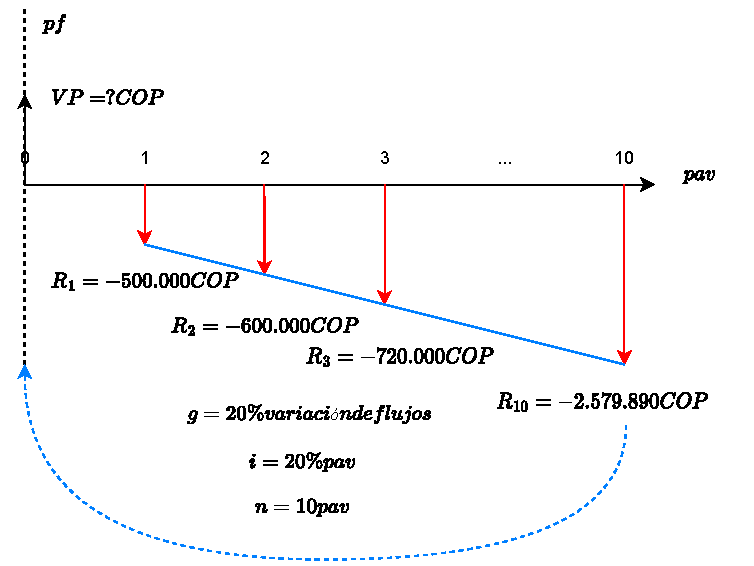
\includegraphics[trim=-5 -5 -5 -5 , scale=0.5]{6_Capitulo/img/ejemplos/7/Capitulo6Ejemplo7.pdf} }
		
		\\ \hline
		%%%%%%%%%%%%% FIN INSERCIÓN DE IMAGEN
		%%%%%FIN FLUJO DE CAJA
		
		%%%%% INICIO DECLARACIÓN FORMULAS
		%%%%%%%%%%% INICIO TITULO
		\rowcolor[HTML]{FFB183}
		\multicolumn{3}{|c|}{\cellcolor[HTML]{FFB183}\textbf{4. Declaración de fórmulas}}    \\ \hline
		%%%%%%%%%%% FIN TITULO
		%%%%%%%%%%% INICIO MATEMÁTICAS
		
		\multicolumn{3}{|c|}{$VP=(\frac{(R)(n)}{1+i}) \hspace{0.4 cm} \textit{Valor presente de un gradiente geometrico para i=g}$} \\ 
		\multicolumn{3}{|c|}{$R_n=(R_1(1+g)^{n-1}) \hspace{0.4 cm} \textit{Valor del flujo de un gradiente geométrico}$} \\ \hline
		
		%%%%%%%%%% FIN MATEMÁTICAS
		%%%%%% INICIO DESARROLLO MATEMÁTICO
		\rowcolor[HTML]{FFB183}
		%%%%%%%%%%INICIO TITULO
		\multicolumn{3}{|c|}{\cellcolor[HTML]{FFB183}\textbf{5. Desarrollo matemático}}       \\ \hline
		%%%%%%%%%% FIN TITULO
		%%%%%%%%%% INICIO MATEMÁTICAS
		
		\multicolumn{3}{|c|}{$VP=(\frac{( 500{.}000COP)(10)}{1+0,2}) \hspace{0.2 cm}\rightarrow \hspace{0.2 cm} VP=  4{.}166{.}667COP$} \\ \hline
		%%%%%%%%%% FIN MATEMÁTICAS
		%%%%%% FIN DESARROLLO MATEMÁTICO
		%%%%%% INICIO RESPUESTA
		\rowcolor[HTML]{FFB183}
		%%%%%%%%%%INICIO TITULO
		\multicolumn{3}{|c|}{\cellcolor[HTML]{FFB183}\textbf{6. Respuesta}}   \\ \hline
		%%%%%%%%%% FIN TITULO
		%%%%%%%%%% INICIO RESPUESTA MATEMÁTICA
		\multicolumn{3}{|c|}{${VP=  4{.}166{.}667 COP}$} 
		\\ \hline
		%%%%%%%%%% FIN MATEMÁTICAS
		%%%%%% FIN RESPUESTA
	\end{longtable}
	%Se crean dos lineas en blanco para que no quede el siguiente texto tan pegado
	%\newline \newline %USARLO SI CREES QUE ES NECESARIO
\end{center}
%%%%%%%%%%%%%%%%%%%%%%%%%%FIN EJERCICIO 7 %%%%%%%%%%%%%%%%%%%%%%%%%%%

\newpage
\textbf{Ejemplo 8}\\
Supongamos que un inversionista desea adquirir la aceptación bancaria del ejemplo anterior, la cual figura con una tasa de registro del 30\% periódico 40 días vencido y con precio de registro $P_r =  97,65 COP$ pero él también sabe que para adquirirla deberá pagar una comisión a un corredor de bolsa lo cual hará variar el precio que él debe pagar y también la rentabilidad que él pueda obtener. Supongamos que la comisión que cobra un corredor por la compra es del 0,475\% periodo 40 días periodo vencido ¿Cuál es el precio del inversionista Pc =  ? COP , que incluye la comisión del comisionista vendedor, el precio de registro y la comisión de bolsa del comprador. El punto de referencia es el precio de registro $P_r$ ¿Cuál es la rentabilidad del inversionista $i_c =? \%?$ periódica 40 días vencido, o $j=? \hspace{0.5mm} nadv$
%\newpage %USAR SOLO SI EL SOLUCIÓN QUEDA SOLO Y ES NECESARIO BAJARLO A LA SIGUIENTE PAGINA

\textbf{Solución.}
%La tabla ira centrada
\begin{center}
 \renewcommand{\arraystretch}{1.5}% Margenes de las celdas
 %Creación de la cuadricula de 3 columnas
 \begin{longtable}[H]{|p{0.5\linewidth}|p{0.5\linewidth}|}
  %Creamos una linea horizontal
  \hline
  %Definimos el color de la primera fila
  \rowcolor[HTML]{FFB183}
  %%%%% INICIO ASIGNACIÓN FECHA FOCAL %%%%%%%
  %%%%%%%%%% INICIO TITULO
  %Lo que se hace aquí es mezclar las 3 columnas en una sola
  \multicolumn{2}{|c|}{\cellcolor[HTML]{FFB183}\textbf{1. Asignación período focal}}                  \\ \hline
  %%%%%%%%%% FIN TITULO
  %%%%% INICIO DECLARACIÓN DE VARIABLES %%%%%%%
  \multicolumn{2}{|c|}{$pf = 40 \textit{ pdv}$}                                                     \\ \hline
  %%%%%%%%%% INICIO TITULO
  %Lo que se hace aquí es mezclar las 3 columnas en una sola
  \multicolumn{2}{|c|}{\cellcolor[HTML]{FFB183}\textbf{2. Declaración de variables}}                \\ \hline
  %%%%%%%%%% FIN TITULO
  %%%%%%%%%% INICIO DE MATEMÁTICAS
  %Cada & hace referencia al paso de la siguiente columna
  $i_c = 30\% -0,475\% = 29,525\% \hspace{1mm} p40dv$ & $P_R=?$                                     \\
  $P_c =  ? COP$                                         &                                             \\
  $n= \frac{40}{365} \hspace{1mm} p(40das) $          &                                             \\ \hline
  %%%%%%%%%% FIN DE MATEMÁTICAS
  %%%%% FIN DECLARACIÓN DE VARIABLES

  \rowcolor[HTML]{FFB183}
  \multicolumn{2}{|c|}{\cellcolor[HTML]{FFB183}\textbf{3. Diagrama de flujo de caja}}               \\ \hline
  \multicolumn{2}{|c|}{ 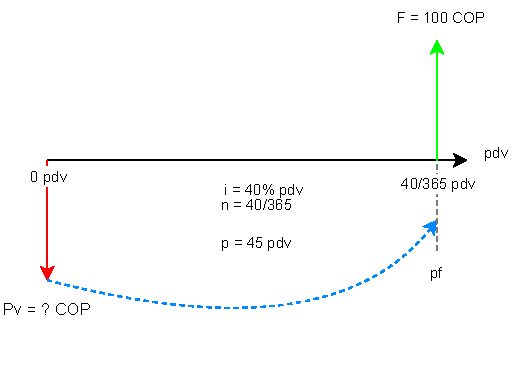
\includegraphics[trim=-78 0 -78 0]{3_Capitulo/img/ejemplos/8/capitulo3ejercicio8.pdf} }  \\ \hline
  %%%%% INICIO FLUJO DE CAJA
  \rowcolor[HTML]{FFB183}
  \multicolumn{2}{|c|}{\cellcolor[HTML]{FFB183}\textbf{4. DECLARACIÓN de formulas}}                 \\ \hline
  %Mezclamos 3 columnas y pondremos el dibujo
  %%%%%%%%%%%%% INSERCIÓN DE LA IMAGEN
  %Deberán descargar las imágenes respectivas del drive y pegarlas en la carpeta
  %n_capitulo/img/ejemplos/1/capitulo1ejemplo1.pdf  (el /1/ es el numero del ejemplo)
  \multicolumn{2}{|c|}{ $P = F(1 + i)^n $ Valor presente }                                          \\ \hline
  %%%%%%%%%%%%% FIN INSERCIÓN DE IMAGEN
  %%%%%FIN FLUJO DE CAJA


  %%%%%% INICIO DESARROLLO MATEMÁTICO
  \rowcolor[HTML]{FFB183}
  %%%%%%%%%%INICIO TITULO
  \multicolumn{2}{|c|}{\cellcolor[HTML]{FFB183}\textbf{5. Desarrollo matemático}}                   \\ \hline
  %%%%%%%%%% FIN TITULO
  %%%%%%%%%% INICIO MATEMÁTICAS
  \multicolumn{2}{|C{\linewidth}|}{
  $P_c =  100 COP(1 + 0,29525)\frac{40}{365} = 97,204 COP$ Ecuación de valor

  $P_R = 0,972047( 5{.}000{.}000 COP) =  4{.}860{.}245 COP$

  $P_c - P_R =  4{.}860{.}235 COP -  4{.}858{.}285 COP = 1{.}950 COP$
  }                                                                                                 \\ \hline

  %%%%%%%%%% FIN MATEMÁTICAS
  %%%%%% FIN DESARROLLO MATEMÁTICO
  %%%%%% INICIO RESPUESTA
  \rowcolor[HTML]{FFB183}
  %%%%%%%%%%INICIO TITULO
  \multicolumn{2}{|c|}{\cellcolor[HTML]{FFB183}\textbf{6. Respuesta}}                               \\ \hline
  %%%%%%%%%% FIN TITULO
  %%%%%%%%%% INICIO RESPUESTA MATEMÁTICA
  \multicolumn{2}{|C{\textwidth}|}{
  $P_R =  4{.}860{.}245 COP$
  }                                                                                                 \\ \hline


  %%%%%%%%%% FIN MATEMÁTICAS
  %%%%%% FIN RESPUESTA
 \end{longtable}
 %Se crean dos lineas en blanco para que no quede el siguiente texto tan pegado
 %\newline \newline %USARLO SI CREES QUE ES NECESARIO
\end{center}
\textbf{Ejemplo 9}\\
Elaborar una tabla para amortizar la suma de  100.000 COP en 4 pagos, suponiendo una tasa del 8\% periódica anual vencida:
\begin{itemize}
	\item a. Crecimiento geométrico periódico de 10\% de los flujos
	\item b. Decrecimiento geométrico periódico de 10\% de los flujos
\end{itemize}
	
	%%%%%%%%%%%%%%%%%%% EJERCICIO 9a %%%%%%

%\newpage %USAR SOLO SI EL SOLUCIÓN QUEDA SOLO Y ES NECESARIO BAJARLO A LA SIGUIENTE PAGINA
\textbf{Solución a.}\\
%La tabla ira centrada
\begin{center}
	\renewcommand{\arraystretch}{1.6}% Margenes de las celdas
	%Creación de la cuadricula de 3 columnas
	\begin{longtable}[H]{|c|c|c|}
		%Creamos una linea horizontal
		\hline
		%Definimos el color de la primera fila
		\rowcolor[HTML]{FFB183}
		%%%%% INICIO ASIGNACIÓN FECHA FOCAL %%%%%%%
		%%%%%%%%%% INICIO TITULO
		%Lo que se hace aquí es mezclar las 3 columnas en una sola
		\multicolumn{3}{|c|}{\cellcolor[HTML]{FFB183}\textbf{1. Asignación período focal}}  \\ \hline
		\multicolumn{3}{|c|}{$pf = \textit{0 pav}$}   \\\hline
		%%%%%%%%%% FIN TITULO
		%%%%% INICIO DECLARACIÓN DE VARIABLES %%%%%%%
		%%%%%%%%%% INICIO TITULO
		%Lo que se hace aquí es mezclar las 3 columnas en una sola
		\multicolumn{3}{|c|}{\cellcolor[HTML]{FFB183}\textbf{2. Declaración de variables}}   \\ \hline
		%%%%%%%%%% FIN TITULO
		%%%%%%%%%% INICIO DE MATEMÁTICAS
		%Cada & hace referencia al paso de la siguiente columna
		\multicolumn{2}{|c|}{$\hspace{2 cm}R=  100{.}000 COP \hspace{2 cm}$} & $i=8\% \textit{ pav}$ \\
		\multicolumn{2}{|c|}{$\hspace{2 cm}n=4  \textit{ pav} \hspace{2 cm}$} & $g=10\% \textit{creicente geometrico periódico con } g \neq i$ \\ \hline	
		
		
		%%%%%%%%%% FIN DE MATEMÁTICAS
		%%%%% FIN DECLARACIÓN DE VARIABLES
		
		%%%%% INICIO FLUJO DE CAJA
		\rowcolor[HTML]{FFB183}
		\multicolumn{3}{|c|}{\cellcolor[HTML]{FFB183}\textbf{3. Diagrama de flujo de caja}} \\ \hline
		%Mezclamos 3 columnas y pondremos el dibujo
		%%%%%%%%%%%%% INSERCIÓN DE LA IMAGEN
		%Deberán descargar las imágenes respectivas del drive y pegarlas en la carpeta
		%n_capitulo/img/ejemplos/1/capitulo1ejemplo1.pdf  (el /1/ es el numero del ejemplo)
		\multicolumn{3}{|c|}{ 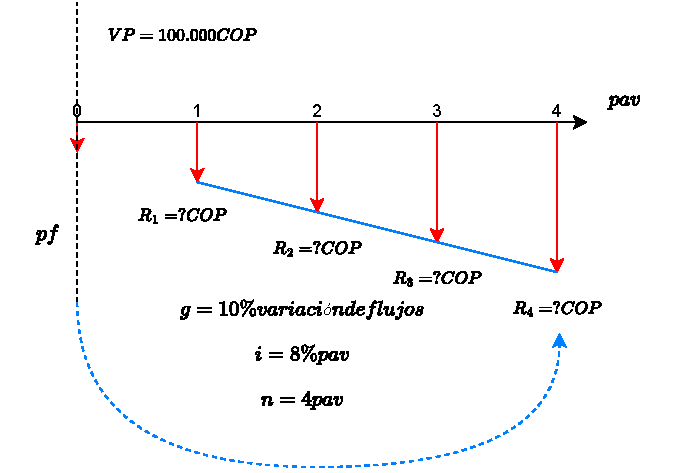
\includegraphics[trim=-5 -5 -5 -5 , scale=0.6]{6_Capitulo/img/ejemplos/9/Capitulo6Ejemplo9a.pdf} }
		\\ \hline
		%%%%%%%%%%%%% FIN INSERCIÓN DE IMAGEN
		%%%%%FIN FLUJO DE CAJA
		
		%%%%% INICIO DECLARACIÓN FORMULAS
		%%%%%%%%%%% INICIO TITULO
		\rowcolor[HTML]{FFB183}
		\multicolumn{3}{|c|}{\cellcolor[HTML]{FFB183}\textbf{4. Declaración de fórmulas}}    \\ \hline
		%%%%%%%%%%% FIN TITULO
		%%%%%%%%%%% INICIO MATEMÁTICAS
		\multicolumn{3}{|c|}{$VP=(\frac{(R)[(1+g)^{n}(1+i)^{-n}-1]}{g-i}) \hspace{0.4 cm} \textit{Valor presente de un gradiente aritmético }$} \\  
		\multicolumn{3}{|c|}{$R_n=(R_1(1+g)^{n-1}) \hspace{0.4 cm} \textit{Valor del flujo de n gradiente geométrico}$} \\ \hline
		
		%%%%%%%%%% FIN MATEMÁTICAS
		%%%%%% INICIO DESARROLLO MATEMÁTICO
		\rowcolor[HTML]{FFB183}
		%%%%%%%%%%INICIO TITULO
		\multicolumn{3}{|c|}{\cellcolor[HTML]{FFB183}\textbf{5. Desarrollo matemático}}       \\ \hline
		%%%%%%%%%% FIN TITULO
		%%%%%%%%%% INICIO MATEMÁTICAS
		\multicolumn{3}{|c|}{$100{.}000COP=(\frac{(R_1)[(1+0.1)^{4}(1+0.08)^{-4}-1]}{0.1-0.08})$} \\
		\multicolumn{3}{|c|}{$R_1=  26{.}261.47 COP$}\\ 
		\multicolumn{3}{|c|}{$R_2=  26{.}261.47(1+0.1) COP=   28{.}887.61COP$}\\
		\multicolumn{3}{|c|}{$R_3=  26{.}261.47(1+0.1)^2 COP=   31{.}776.38COP$}\\
		\multicolumn{3}{|c|}{$R_4=  26{.}261.47(1+0.1)^3 COP=   34{.}954.01COP$}\\ \hline
		%%%%%%%%%% FIN MATEMÁTICAS
		%%%%%% FIN DESARROLLO MATEMÁTICO
		%%%%%% INICIO RESPUESTA
		\rowcolor[HTML]{FFB183}
		%%%%%%%%%%INICIO TITULO
		\multicolumn{3}{|c|}{\cellcolor[HTML]{FFB183}\textbf{6. Respuesta}}   \\ \hline
		%%%%%%%%%% FIN TITULO
		%%%%%%%%%% INICIO RESPUESTA MATEMÁTICA
		\multicolumn{3}{|c|}{$R_1=  26{.}261COP$}\\ 
		\multicolumn{3}{|c|}{$R_2=  28{.}888 COP$}\\
		\multicolumn{3}{|c|}{$R_3=  31{.}776 COP$}\\
		\multicolumn{3}{|c|}{$R_4=  34{.}954 COP$}\\ \hline
		%%%%%%%%%% FIN MATEMÁTICAS
		%%%%%% FIN RESPUESTA
	\end{longtable}
	%Se crean dos lineas en blanco para que no quede el siguiente texto tan pegado
	%\newline \newline %USARLO SI CREES QUE ES NECESARIO
\end{center}

%%%%%%%%%%%%%%%%%%%%%%%%%%FIN EJERCICIO 9a %%%%%%%%%%%%%%%%%%%%%%%%%%%
	      \begin{spacing}{1.1}
	      	\begin{center}
	      		\begin{tabular}{|p{1cm}|p{2cm}|p{2.1cm}|p{2cm}|p{3cm}|}
	      			\hline
	      			\rowcolor{white!50}
	      			\textbf{n\ } & \textbf{Saldo Deuda COP} & \textbf{Intereses  COP} & \textbf{Pago COP} & \textbf{Amortización COP } \\ \hline
	      			
	      			0            &   100.000         &      -       &   -    &        -      \\ \hline
	      			1            &   81.739             &   8.000           &   26.261       &   18.261            \\ \hline
	      			2            &   59.390             &   6539,13              &   28.888       &   22.348,88              \\ \hline
	      			3            &   32.365.21            &   4751,2             &   31.776      &   27.024,79              \\ \hline
	      			4            &   0            &   2589,22            &   34.954       &   32.365,21              \\ \hline
	      		\end{tabular}
	      	\end{center}
	      \end{spacing}

	%%%%%%%%%%%%%%%%%%% EJERCICIO 9b %%%%%%

%\newpage %USAR SOLO SI EL SOLUCIÓN QUEDA SOLO Y ES NECESARIO BAJARLO A LA SIGUIENTE PAGINA
\textbf{Solución b.}\\
%La tabla ira centrada
\begin{center}
	\renewcommand{\arraystretch}{1.6}% Margenes de las celdas
	%Creación de la cuadricula de 3 columnas
	\begin{longtable}[H]{|c|c|c|}
		%Creamos una linea horizontal
		\hline
		%Definimos el color de la primera fila
		\rowcolor[HTML]{FFB183}
		%%%%% INICIO ASIGNACIÓN FECHA FOCAL %%%%%%%
		%%%%%%%%%% INICIO TITULO
		%Lo que se hace aquí es mezclar las 3 columnas en una sola
		\multicolumn{3}{|c|}{\cellcolor[HTML]{FFB183}\textbf{1. Asignación período focal}}  \\ \hline
		\multicolumn{3}{|c|}{$pf = \textit{0 pav}$}   \\\hline
		%%%%%%%%%% FIN TITULO
		%%%%% INICIO DECLARACIÓN DE VARIABLES %%%%%%%
		%%%%%%%%%% INICIO TITULO
		%Lo que se hace aquí es mezclar las 3 columnas en una sola
		\multicolumn{3}{|c|}{\cellcolor[HTML]{FFB183}\textbf{2. Declaración de variables}}   \\ \hline
		%%%%%%%%%% FIN TITULO
		%%%%%%%%%% INICIO DE MATEMÁTICAS
		%Cada & hace referencia al paso de la siguiente columna
		\multicolumn{2}{|c|}{$\hspace{2 cm}VP= 100{.}000 COP \hspace{2 cm}$} & $i=8\% \textit{ pav}$ \\
		\multicolumn{2}{|c|}{$\hspace{2 cm}n=4  \textit{ pav} \hspace{2 cm}$} & $g=-10\% \textit{decreicente con } g \neq i$ \\ \hline	
		
		%%%%%%%%%% FIN DE MATEMÁTICAS
		%%%%% FIN DECLARACIÓN DE VARIABLES
		
		%%%%% INICIO FLUJO DE CAJA
		\rowcolor[HTML]{FFB183}
		\multicolumn{3}{|c|}{\cellcolor[HTML]{FFB183}\textbf{3. Diagrama de flujo de caja}} \\ \hline
		%Mezclamos 3 columnas y pondremos el dibujo
		%%%%%%%%%%%%% INSERCIÓN DE LA IMAGEN
		%Deberán descargar las imágenes respectivas del drive y pegarlas en la carpeta
		%n_capitulo/img/ejemplos/1/capitulo1ejemplo1.pdf  (el /1/ es el numero del ejemplo)
		\multicolumn{3}{|c|}{ 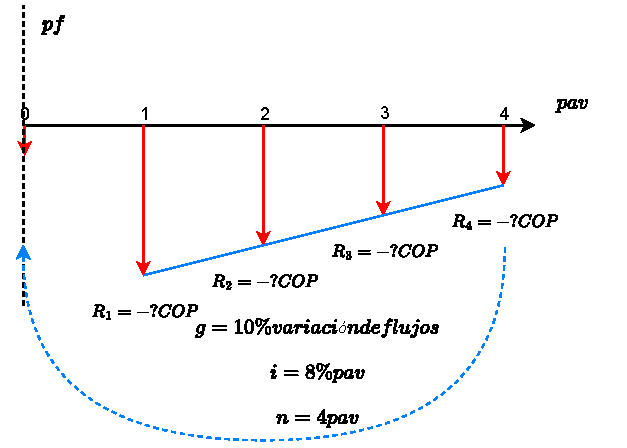
\includegraphics[trim=-5 -5 -5 -5 , scale=0.6]{6_Capitulo/img/ejemplos/9/Capitulo6Ejemplo9b.pdf} }
		\\ \hline
		%%%%%%%%%%%%% FIN INSERCIÓN DE IMAGEN
		%%%%%FIN FLUJO DE CAJA
		
		%%%%% INICIO DECLARACIÓN FORMULAS
		%%%%%%%%%%% INICIO TITULO
		\rowcolor[HTML]{FFB183}
		\multicolumn{3}{|c|}{\cellcolor[HTML]{FFB183}\textbf{4. Declaración de fórmulas}}    \\ \hline
		%%%%%%%%%%% FIN TITULO
		%%%%%%%%%%% INICIO MATEMÁTICAS
		\multicolumn{3}{|c|}{$VP=(\frac{(R)[(1+g)^{n}(1+i)^{-n}-1]}{g-i}) \hspace{0.4 cm} \textit{Valor presente de un gradiente aritmético }$} \\  
		\multicolumn{3}{|c|}{$R_n=(R_1(1+g)^{n-1}) \hspace{0.4 cm} \textit{Valor del flujo de n gradiente geométrico}$} \\ \hline
		
		%%%%%%%%%% FIN MATEMÁTICAS
		%%%%%% INICIO DESARROLLO MATEMÁTICO
		\rowcolor[HTML]{FFB183}
		%%%%%%%%%%INICIO TITULO
		\multicolumn{3}{|c|}{\cellcolor[HTML]{FFB183}\textbf{5. Desarrollo matemático}}       \\ \hline
		%%%%%%%%%% FIN TITULO
		%%%%%%%%%% INICIO MATEMÁTICAS
		\multicolumn{3}{|c|}{$  100{.}000COP=(\frac{(R_1)[(1-0.1)^{4}(1+0.08)^{-4}-1]}{-0.1-0.08})$} \\
		\multicolumn{3}{|c|}{$R_1=  34{.}766 COP$}\\ 
		\multicolumn{3}{|c|}{$R_2=  34{.}766.02COP(1-0.1)  =   31{.}289.42COP$}\\
		\multicolumn{3}{|c|}{$R_3=  34{.}766.02COP(1-0.1)^2 =   28{.}160.48COP$}\\
		\multicolumn{3}{|c|}{$R_4=  34{.}766.02COP(1-0.1)^3 =   25{.}344.43COP$}\\ \hline
		%%%%%%%%%% FIN MATEMÁTICAS
		%%%%%% FIN DESARROLLO MATEMÁTICO
		%%%%%% INICIO RESPUESTA
		\rowcolor[HTML]{FFB183}
		%%%%%%%%%%INICIO TITULO
		\multicolumn{3}{|c|}{\cellcolor[HTML]{FFB183}\textbf{6. Respuesta}}   \\ \hline
		%%%%%%%%%% FIN TITULO
		%%%%%%%%%% INICIO RESPUESTA MATEMÁTICA
		\multicolumn{3}{|c|}{$R_1=  34{.}766COP$}\\ 
		\multicolumn{3}{|c|}{$R_2=  31{.}289COP$}\\
		\multicolumn{3}{|c|}{$R_3=  28{.}160COP$}\\
		\multicolumn{3}{|c|}{$R_4=  25{.}344COP$}\\ \hline
		%%%%%%%%%% FIN MATEMÁTICAS
		%%%%%% FIN RESPUESTA
	\end{longtable}
	%Se crean dos lineas en blanco para que no quede el siguiente texto tan pegado
	%\newline \newline %USARLO SI CREES QUE ES NECESARIO
\end{center}

%%%%%%%%%%%%%%%%%%%%%%%%%%FIN EJERCICIO 9b %%%%%%%%%%%%%%%%%%%%%%%%%%%
	      
	      \begin{spacing}{1.1}
		      \begin{center}
			      \begin{tabular}{|p{1cm}|p{2cm}|p{2.1cm}|p{2cm}|p{2.5cm}|}
				      \hline
				      \rowcolor{white!50}
				      \textbf{n\ } & \textbf{Saldo Deuda COP} & \textbf{Intereses COP } & \textbf{Pago COP } & \textbf{Amortización COP} \\ \hline
				      
				      0            &   100.000         & -    & -  & -    \\ \hline
				      1            &   73.234           &   8.000          &   34.766      &   26.766             \\ \hline
				      2            &   47.803,72           &   5858,72             &   31.289      &   25.430,28             \\ \hline
				      3            &   23.468,01           &   3824,29             &   28.160      &   24.335,7            \\ \hline
				      4            &   0               &   1877,44             &   25.344,73      &   23.468,01             \\ \hline
			      \end{tabular}
		      \end{center}
	      \end{spacing}

%%%%%%%%%%%%%%%%%%%%%%%%%%EJERCICIO 10 %%%%%%%%%%%%%%%%%%%%%%%%%%%
 \textbf{Ejemplo 10}\\
	Resolver el problema anterior, suponiendo que el gradiente es escalonado con pagos semestrales.\\		
	
	\textbf{Solución 10}\\
	%La tabla ira centrada
	\begin{center}
		\renewcommand{\arraystretch}{1.5}% Margenes de las celdas
		%Creación de la cuadricula de 3 columnas
		\begin{longtable}[H]{|p{0.5\linewidth}|p{0.5\linewidth}|}
			%Creamos una linea horizontal
			\hline
			%Definimos el color de la primera fila
			\rowcolor[HTML]{FFB183}
			%%%%% INICIO ASIGNACIÓN período FOCAL %%%%%%%
			%%%%%%%%%% INICIO TITULO
			%Lo que se hace aquí es mezclar las 3 columnas en una sola
			\multicolumn{2}{|c|}{\cellcolor[HTML]{FFB183}\textbf{1. Asignación período focal}}   \\ \hline
			%%%%%%%%%% FIN TITULO
			%%%%% INICIO DECLARACIÓN DE VARIABLES %%%%%%%
			\multicolumn{2}{|c|}{$pf = 0 \textit{ psv}$}\\ \hline
			%%%%%%%%%% INICIO TITULO
			%Lo que se hace aquí es mezclar las 3 columnas en una sola
			\multicolumn{2}{|c|}{\cellcolor[HTML]{FFB183}\textbf{2. Declaración de variables}}   \\ \hline
			%%%%%%%%%% FIN TITULO
			%%%%%%%%%% INICIO DE MATEMÁTICAS
			%Cada & hace referencia al paso de la siguiente columna
			$VP = 500.000 \ COP $  				& $ n_{2}= 2 \hspace{1mm} psv $  \\
			$i \equiv  10\% \hspace{1mm} pav$      	& $ n_{3}= 3 \hspace{1mm} psv $ \\
			$ n = 2 \hspace{1mm} psv $          & $ n_{5}= 5 \hspace{1mm} psv $\\ 
			$ n_{1}= 1 \hspace{1mm} psv $       & $ n_{6}= 6 \hspace{1mm} psv $ \\ 
			$ $      						    & $ i \equiv  ? \% psv $ \\ \hline
			%%%%%%%%%% FIN DE MATEMÁTICAS
			%%%%% FIN DECLARACIÓN DE VARIABLES
			
			\rowcolor[HTML]{FFB183}
			\multicolumn{2}{|c|}{\cellcolor[HTML]{FFB183}\textbf{3. Diagrama de flujo de caja}} \\ \hline
			\multicolumn{2}{|c|}{ 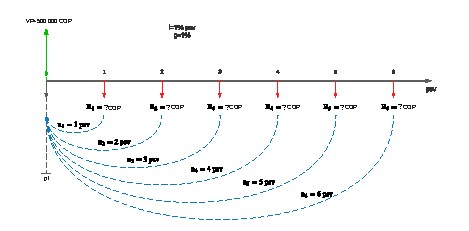
\includegraphics[trim=-78 -5 -78 -5]{7_Capitulo/img/ejemplos/10/10_1.pdf} }   \\ \hline
			%%%%% INICIO FLUJO DE CAJA
			\rowcolor[HTML]{FFB183}
			\multicolumn{2}{|c|}{\cellcolor[HTML]{FFB183}\textbf{4. Declaración de fórmulas}} \\ \hline
			%%%%%%%%%%%%% FIN INSERCIÓN DE IMAGEN
			%%%%%FIN FLUJO DE CAJA
			
			\multicolumn{2}{|c|}{ $(1+i_1)^{m_1} = (1+i_2)^{m_2} $ Equivalencia de tasas}   \\  
			\multicolumn{2}{|c|}{ $VF = R\frac{(1+i)^{n} -1 }{i} $ Valor presente serie uniforme}   \\  \hline
			
			%%%%%% INICIO DESARROLLO MATEMÁTICO
			\rowcolor[HTML]{FFB183}
			%%%%%%%%%%INICIO TITULO
			\multicolumn{2}{|c|}{\cellcolor[HTML]{FFB183}\textbf{5. Desarrollo matemático}}       \\ \hline
			%%%%%%%%%% FIN TITULO
			%%%%%%%%%% INICIO MATEMÁTICAS
			\multicolumn{2}{|c|}{  $(1+ 0,24)^{1} = (1+i)^{2} $}   \\ 
			\multicolumn{2}{|c|}{ $  i = 11,3552873\% \hspace{1mm} psv $}   \\  \hline
			
			%%%%%%%%%% FIN MATEMÁTICAS
			%%%%%% FIN DESARROLLO MATEMÁTICO
			%%%%%% INICIO RESPUESTA
			\rowcolor[HTML]{FFB183}
			%%%%%%%%%%INICIO TITULO
			\multicolumn{2}{|c|}{\cellcolor[HTML]{FFB183}\textbf{6. Respuesta}}   \\ \hline
			%%%%%%%%%% FIN TITULO
			%%%%%%%%%% INICIO RESPUESTA MATEMÁTICA
			\multicolumn{2}{|c|}{ 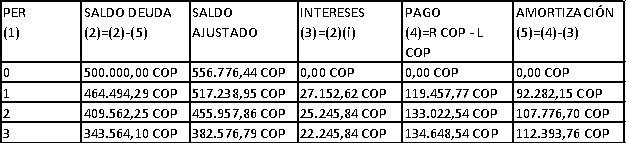
\includegraphics[trim=-78 -5 -78 -5]{7_Capitulo/img/ejemplos/10/10_2.pdf} }   \\ \hline
			%\multicolumn{2}{|C{\textwidth}|}{
			%	$R_{58} = 72.478,16 \ COP (1 + 0,02)^{57} = \ COP 224.087,15 $ 
			%}  \\ \hline
			
			
			%%%%%%%%%% FIN MATEMÁTICAS
			%%%%%% FIN RESPUESTA
		\end{longtable}
		%Se crean dos lineas en blanco para que no quede el siguiente texto tan pegado
		%\newline \newline %USARLO SI CREES QUE ES NECESARIO
	\end{center}
 %%%%%%%%%%%%%%%%%%%%%%%%%%FIN EJERCICIO 10 %%%%%%%%%%%%%%%%%%%%%%%%%%%

\section{Ecuaciones de equivalencia de flujos}
Es muy frecuente cambiar una o varias obligaciones por otra u otras nuevas obligaciones. La solución de este problema es elemental y para solucionarlo es necesario usar la ecuación de equivalencia de flujos, que es una igualdad de valores ubicados en una sola fecha denominada período focal.\\
La período focal se representa gráficamente por una línea a trazos y por las letras pf y es la fecha en que debe hacerse la igualdad entre ingresos (flujos positivos) y egresos (flujos negativos) . La ubicación de la período focal no altera la respuesta final, por tal motivo se deja a libre elección de la persona que va a resolver el problema.\\
El principio fundamental de una ecuación de valor, que viene a ser el mismo principio fundamental de las finanzas, establece que la sumatoria de los ingresos debe ser igual a la sumatoria de los egresos ubicados ambos en la período focal, esto es:

\begin{center}
   $\sum ingresos = \sum egresos(en\ la\ pf)$\\
\end{center}
Naturalmente, para el traslado de cada una de las cantidades a la período focal, debe hacerse usando la fórmula de valor futuro.\\
El enunciado de una ecuación de equivalencia también puede ser expresado así:

\begin{center}
   $\sum deudas = \sum pagos(en\ la\ pf)$\\
\end{center}

Mirando un balance el principio puede ser expresado así:\\

\begin{center}
   $\sum activos = \sum pasivos + capital(en\ la\ pf)$\\
\end{center}

Como en cualquier proyecto, los ingresos se representan por flechas hacia arriba y los egresos por flechas hacia abajo, entonces, mirando la gráfica de flujo de caja podemos expresar el principio fundamental de una ecuación de equivalencia de flujos de esta otra forma:\\

\begin{center}
   $\sum de\ lo\ que\ $\textit{está}$\ para\ arriba = \sum de\ lo\ que\ $\textit{está}$\ para\ abajo(en\ la\ pf)$\\
\end{center}

La sumatoria de los ingresos en pesos de hoy menos la sumatoria de los egresos en pesos de hoy recibe el nombre de valor presente neto (VPN) o valor actual neto.\\
La tasa a la cual la sumatoria de los ingresos (VPN) es igual a la sumatoria de los egresos (en la período focal) se denomina tasa interna de retorno (TIR).\\
En el capítulo posterior analizaremos con más detalle los conceptos de VPN y TIR, estos conceptos son de suma importancia en la evaluación de proyectos.\\

\textbf{Ejemplo 11}\\
Hallar el valor presente de 15 pagos que decrecen
linealmente en 400 COP, si el primer pago es de 5.000 COP y la tasa efectiva es del 4\% período año
vencido..\\ \\
%\newpage %USAR SOLO SI EL SOLUCIÓN QUEDA SOLO Y ES NECESARIO BAJARLO A LA SIGUIENTE PAGINA
\textbf{Solución.}\\
%La tabla ira centrada
\begin{center}
 \renewcommand{\arraystretch}{1.5}% Margenes de las celdas
 %Creación de la cuadricula de 3 columnas
 \begin{longtable}[H]{|p{0.5\linewidth}|p{0.5\linewidth}|}
  \hline
  \multicolumn{2}{|c|}{\cellcolor[HTML]{FFB183}\textbf{1. Declaración de variables}}                                                                                                                 \\ \hline
  $R =  5.400 COP$                                                                                & $L = 400 COP$                                                                                   \\
  $n=15 \hspace{1mm} pav$                                                                         & $VP=? COP$                                                                                         \\
  $i=4,0\% \hspace{1mm} pav$                                                                      &                                                                                                  \\
  \multicolumn{2}{|c|}{\cellcolor[HTML]{FFB183}\textbf{2. Diagrama de flujo de caja}}                                                                                                                \\ \hline
  \multicolumn{1}{|c|}{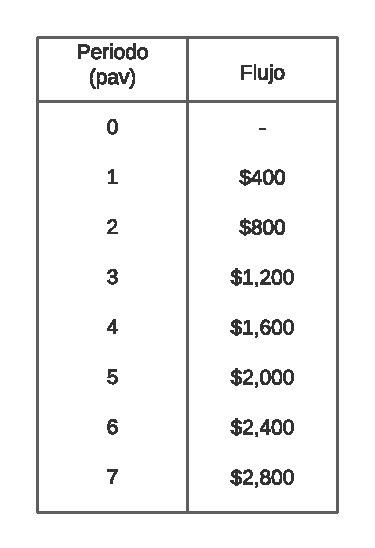
\includegraphics[trim=-5 -5 -5 -5 ,width=0.5\columnwidth]{11/Tabla 1.pdf}} & \multicolumn{1}{|c|}{ \includegraphics[trim=-5 -5 -5 -5 ,width=0.5\columnwidth]{11/Tabla 2.pdf}} \\ \hline
  \multicolumn{2}{|c|}{\cellcolor[HTML]{FFB183}\textbf{3. Aplicación de funciones}}                                                                                                                  \\ \hline
  \multicolumn{2}{|p{\columnwidth}|}{Se aplicará la función valor presente VNA de la siguiente forma: \newline
  =VNA(0,04;J8::J22) con referencia en la hoja de
  Excel usada para el ejercicio.}                                                                                                                                                                    \\
  \multicolumn{2}{|c|}{ \includegraphics[trim=-5 -5 -5 -5 ,width=0.7\columnwidth]{11/excel1.png}}                                                                                                    \\ \hline
  \multicolumn{2}{|c|}{\cellcolor[HTML]{FFB183}\textbf{4. Gráfica}}                                                                                                                                  \\ \hline
  \multicolumn{2}{|c|}{ \includegraphics[trim=-5 -5 -5 -5 ,width=0.8\columnwidth]{11/gráfico.pdf}}                                                                                                   \\ \hline
  \multicolumn{2}{|c|}{\cellcolor[HTML]{FFB183}\textbf{5. Respuesta}}                                                                                                                                \\ \hline
  \multicolumn{2}{|c|}{El valor presente es VP =  COP 27.697,9410}                                                                                                                                      \\ \hline
 \end{longtable}
 %\newline \newline %USARLO SI CREES QUE ES NECESARIO
\end{center}


\textbf{Ejemplo 12}\\
Hallar el valor presente de una serie infinita de egresos que crecen en un 10\%, si la tasa de interés es del 20\% pav y el primer egreso es  300.000COP.\\


%%%%%%%%%%%%%%%%%%% EJERCICIO 12 %%%%%%

%\newpage %USAR SOLO SI EL SOLUCIÓN QUEDA SOLO Y ES NECESARIO BAJARLO A LA SIGUIENTE PAGINA
\textbf{Solución.}\\
%La tabla ira centrada
\begin{center}
	\renewcommand{\arraystretch}{1.6}% Margenes de las celdas
	%Creación de la cuadricula de 3 columnas
	\begin{longtable}[H]{|c|c|c|}
		%Creamos una linea horizontal
		\hline
		%Definimos el color de la primera fila
		\rowcolor[HTML]{FFB183}
		%%%%% INICIO ASIGNACIÓN FECHA FOCAL %%%%%%%
		%%%%%%%%%% INICIO TITULO
		%Lo que se hace aquí es mezclar las 3 columnas en una sola
		\multicolumn{3}{|c|}{\cellcolor[HTML]{FFB183}\textbf{1. Asignación período focal}}  \\ \hline
		\multicolumn{3}{|c|}{$pf = \textit{0 pav}$}   \\\hline
		%%%%%%%%%% FIN TITULO
		%%%%% INICIO DECLARACIÓN DE VARIABLES %%%%%%%
		%%%%%%%%%% INICIO TITULO
		%Lo que se hace aquí es mezclar las 3 columnas en una sola
		\multicolumn{3}{|c|}{\cellcolor[HTML]{FFB183}\textbf{2. Declaración de variables}}   \\ \hline
		%%%%%%%%%% FIN TITULO
		%%%%%%%%%% INICIO DE MATEMÁTICAS
		%Cada & hace referencia al paso de la siguiente columna
		\multicolumn{2}{|c|}{\textbf{$\hspace{3.5 cm}\textit{}\hspace{3.5 cm}$}} & \textbf{$\hspace{3.5 cm}\textit{}\hspace{3.5 cm}$} \\ 
		\multicolumn{2}{|c|}{$\hspace{2 cm}R=  300{.}000COP \hspace{2 cm}$} & $i=20\% \textit{ pav}$ \\
		\multicolumn{2}{|c|}{$\hspace{2 cm}n_1=10  \textit{ pav} \hspace{2 cm}$} & $g=10\% \textit{creciente entre flujos} $ \\
		\multicolumn{2}{|c|}{$\hspace{2 cm}VF= ?COP \hspace{2 cm}$} &  \\ \hline	
		
		%%%%%%%%%% FIN DE MATEMÁTICAS
		%%%%% FIN DECLARACIÓN DE VARIABLES
		
		%%%%% INICIO FLUJO DE CAJA
		\rowcolor[HTML]{FFB183}
		\multicolumn{3}{|c|}{\cellcolor[HTML]{FFB183}\textbf{3. Diagrama de flujo de caja}} \\ \hline
		%Mezclamos 3 columnas y pondremos el dibujo
		%%%%%%%%%%%%% INSERCIÓN DE LA IMAGEN
		%Deberán descargar las imágenes respectivas del drive y pegarlas en la carpeta
		%n_capitulo/img/ejemplos/1/capitulo1ejemplo1.pdf  (el /1/ es el numero del ejemplo)
		\multicolumn{3}{|c|}{ \includegraphics[trim=-5 -5 -5 -5 , scale=0.9]{6_Capitulo/img/ejemplos/12/Capitulo6Ejemplo12.pdf} }
		\\ \hline
		%%%%%%%%%%%%% FIN INSERCIÓN DE IMAGEN
		%%%%%FIN FLUJO DE CAJA
		
		%%%%% INICIO DECLARACIÓN FORMULAS
		%%%%%%%%%%% INICIO TITULO
		\rowcolor[HTML]{FFB183}
		\multicolumn{3}{|c|}{\cellcolor[HTML]{FFB183}\textbf{4. Declaración de fórmulas}}    \\ \hline
		%%%%%%%%%%% FIN TITULO
		%%%%%%%%%%% INICIO MATEMÁTICAS
		\multicolumn{3}{|c|}{$VP=(\frac{R}{i-g}) \hspace{0.4 cm} \textit{Valor gradiente si geométrico infinito si g<1} $} \\   \hline
		
		%%%%%%%%%% FIN MATEMÁTICAS
		%%%%%% INICIO DESARROLLO MATEMÁTICO
		\rowcolor[HTML]{FFB183}
		%%%%%%%%%%INICIO TITULO
		\multicolumn{3}{|c|}{\cellcolor[HTML]{FFB183}\textbf{5. Desarrollo matemático}}       \\ \hline
		%%%%%%%%%% FIN TITULO
		%%%%%%%%%% INICIO MATEMÁTICAS
		\multicolumn{3}{|c|}{$VP=(\frac{  300{.}000COP}{0.2-0.1}) \hspace{0.2 cm}\rightarrow \hspace{0.2 cm} VP= 300{.}000 COP$} \\  \hline
		%%%%%%%%%% FIN MATEMÁTICAS
		%%%%%% FIN DESARROLLO MATEMÁTICO
		%%%%%% INICIO RESPUESTA
		\rowcolor[HTML]{FFB183}
		%%%%%%%%%%INICIO TITULO
		\multicolumn{3}{|c|}{\cellcolor[HTML]{FFB183}\textbf{6. Respuesta}}   \\ \hline
		%%%%%%%%%% FIN TITULO
		%%%%%%%%%% INICIO RESPUESTA MATEMÁTICA
		\multicolumn{3}{|c|}{${VP=  300.000 COP }$} \\ \hline
		%%%%%%%%%% FIN MATEMÁTICAS
		%%%%%% FIN RESPUESTA
	\end{longtable}
	%Se crean dos lineas en blanco para que no quede el siguiente texto tan pegado
	%\newline \newline %USARLO SI CREES QUE ES NECESARIO
\end{center}

%%%%%%%%%%%%%%%%%%%%%%%%%%FIN EJERCICIO 12 %%%%%%%%%%%%%%%%%%%%%%%%%%%

	%%%%%%%%%%%%%%%%%%%%%%%%%%EJERCICIO 13 %%%%%%%%%%%%%%%%%%%%%%%%%%%%%%%%%%%%%%%%%%%%%%%%%%%%%%
    \textbf{Ejemplo 13}\\
	
	Una cuota inicial del 30\% y el saldo será pagadero al final de 3 años, mientras tanto se pagarán intereses por período mes anticipado al 3\%. Con el objeto de cancelar la deuda a su vencimiento, se constituye un fondo que paga el 33\% nominal anual mes vencido mediante depósitos mensuales ordinarios crecientes en 2.000 COP. Determinar el costo del período 15.\\
	
	\textbf{Solución 13}\\
	%La tabla ira centrada
	\begin{center}
		\renewcommand{\arraystretch}{1.5}% Margenes de las celdas
		%Creación de la cuadricula de 3 columnas
		\begin{longtable}[H]{|p{0.5\linewidth}|p{0.5\linewidth}|}
			%Creamos una linea horizontal
			\hline
			%Definimos el color de la primera fila
			\rowcolor[HTML]{FFB183}
			%%%%% INICIO ASIGNACIÓN período FOCAL %%%%%%%
			%%%%%%%%%% INICIO TITULO
			%Lo que se hace aquí es mezclar las 3 columnas en una sola
			\multicolumn{2}{|c|}{\cellcolor[HTML]{FFB183}\textbf{1. Asignación período focal}}   \\ \hline
			%%%%%%%%%% FIN TITULO
			%%%%% INICIO DECLARACIÓN DE VARIABLES %%%%%%%
			\multicolumn{2}{|c|}{$pf = 36 \textit{ pmv}$}\\ \hline
			%%%%%%%%%% INICIO TITULO
			%Lo que se hace aquí es mezclar las 3 columnas en una sola
			\multicolumn{2}{|c|}{\cellcolor[HTML]{FFB183}\textbf{2. Declaración de variables}}   \\ \hline
			%%%%%%%%%% FIN TITULO
			%%%%%%%%%% INICIO DE MATEMÁTICAS
			%Cada & hace referencia al paso de la siguiente columna
			$  Interés = 4.200.000 \ COP (0,03) = 126.000 \ COP $  			 \\ \hline
			%%%%%%%%%% FIN DE MATEMÁTICAS
			%%%%% FIN DECLARACIÓN DE VARIABLES
			
			\rowcolor[HTML]{FFB183}
			\multicolumn{2}{|c|}{\cellcolor[HTML]{FFB183}\textbf{3. Diagrama de flujo de caja}} \\ \hline
			\multicolumn{2}{|c|}{ \includegraphics[trim=-78 -5 -78 -5]{7_Capitulo/img/ejemplos/13/13_1.pdf} }   \\
			\multicolumn{2}{|c|}{ \includegraphics[trim=-78 -5 -78 -5]{7_Capitulo/img/ejemplos/13/13_2.pdf} }   \\ \hline
			%%%%% INICIO FLUJO DE CAJA
			\rowcolor[HTML]{FFB183}
			\multicolumn{2}{|c|}{\cellcolor[HTML]{FFB183}\textbf{4. Declaración de fórmulas}} \\ \hline
			%%%%%%%%%%%%% FIN INSERCIÓN DE IMAGEN
			%%%%%FIN FLUJO DE CAJA
			\multicolumn{2}{|c|}{ $VF = R n(1+i)^{n-1} $ \hspace{1mm} Formula del valor futuro gradiente geométrico si g=i}\\    
			\multicolumn{2}{|c|}{ $R_{n} = R_{1} + (n-1)L $ \hspace{1mm} Valor de un periodo aritmetico en un periodo n}   \\ \hline
			
			%%%%%% INICIO DESARROLLO MATEMÁTICO
			\rowcolor[HTML]{FFB183}
			%%%%%%%%%%INICIO TITULO
			\multicolumn{2}{|c|}{\cellcolor[HTML]{FFB183}\textbf{5. Desarrollo matemático}}       \\ \hline
			%%%%%%%%%% FIN TITULO
			%%%%%%%%%% INICIO MATEMÁTICAS
			\multicolumn{2}{|c|}{  $ 4.200.000 \ COP = R_{1} (36) (0,0275) + \frac{ 2.000 \ COP }{0,0275} ((36)(0,0275)-36) $}   \\ 
			\multicolumn{2}{|c|}{  $  R_{1} = 40.531,73 \ COP $}   \\ 
			\multicolumn{2}{|c|}{ $  R_{15} = 40.531,73 \ COP +  ( 15 - 1) (2.000 \ COP) = 68.531,73 \ COP $}   \\  \hline
			
			%%%%%%%%%% FIN MATEMÁTICAS
			%%%%%% FIN DESARROLLO MATEMÁTICO
			%%%%%% INICIO RESPUESTA
			\rowcolor[HTML]{FFB183}
			%%%%%%%%%%INICIO TITULO
			\multicolumn{2}{|c|}{\cellcolor[HTML]{FFB183}\textbf{6. Respuesta}}   \\ \hline
			%%%%%%%%%% FIN TITULO
			%%%%%%%%%% INICIO RESPUESTA MATEMÁTICA
			%\multicolumn{2}{|c|}{ \includegraphics[trim=-78 -5 -78 -5]{7_Capitulo/img/ejemplos/12/12_2.jpg} }   \\ \hline
			\multicolumn{2}{|C{\textwidth}|}{
				$  R_{1} = 40.531,73 \ COP \hspace{2mm} y  \hspace{2mm} R_{15} = 68.531,73 \ COP $
				
				Esto significa que en el período 15 el deudor debe disponer de 194.531,73 COP de los cuales 126.000 COP los dedica al pago de intereses y el resto (68.531,73 COP) se deposita en el fondo.
				
			}  \\ \hline
			
			
			%%%%%%%%%% FIN MATEMÁTICAS
			%%%%%% FIN RESPUESTA
		\end{longtable}
		%Se crean dos lineas en blanco para que no quede el siguiente texto tan pegado
		%\newline \newline %USARLO SI CREES QUE ES NECESARIO
	\end{center}
%%%%%%%%%%%%%%%%%%%%%%%%%%FIN EJERCICIO 13
%%%%%%%%%%%%%%%%%%%% EJERCICIO 14 %%%%%%

\textbf{Ejemplo 14}\\
Una persona debe pagar 70.000 COP en 3 meses y 85.000 COP en 8 meses; ante la imposibilidad de cancelar las deudas en las fechas previstas le ofrece al acreedor que le cancelara 50.000 COP en 4 meses y 130.000 COP en 12 meses. Si el acreedor acepta esta nueva forma de pago ¿Qué tasa de interés periódica mes vencido estará pagando?.\\ \\
\setlength{\parskip}{-1mm}
%\newpage %USAR SOLO SI EL SOLUCIÓN QUEDA SOLO Y ES NECESARIO BAJARLO A LA SIGUIENTE PAGINA
\textbf{Solución.}
%La tabla ira centrada

\begin{center}
  \renewcommand{\arraystretch}{1.5}% Margenes de las celdas
  %Creación de la cuadricula de 3 columnas
  \begin{longtable}[H]{|c|c|c|}
    %Creamos una linea horizontal
    \hline
    %Definimos el color de la primera fila
    \rowcolor[HTML]{FFB183}
    %%%%% INICIO ASIGNACIÓN PERíODO FOCAL %%%%%%%
    %%%%%%%%%% INICIO TITULO
    %Lo que se hace aquí es mezclar las 3 columnas en una sola
    \multicolumn{3}{|c|}{\cellcolor[HTML]{FFB183}\textbf{1. Asignación período focal}}                                                      \\ \hline
    \multicolumn{3}{|c|}{\textbf{ $pf = \textit{ período focal: 0 pmv} $}}                                                                  \\ \hline
    %%%%%%%%%% FIN TITULO
    %%%%% INICIO DECLARACIÓN DE VARIABLES %%%%%%%
    %%%%%%%%%% INICIO TITULO
    %Lo que se hace aquí es mezclar las 3 columnas en una sola
    \multicolumn{3}{|c|}{\cellcolor[HTML]{FFB183}\textbf{2. Declaración de variables}}                                                      \\ \hline
    %%%%%%%%%% FIN TITULO
    %%%%%%%%%% INICIO DE MATEMÁTICAS
    %Cada & hace referencia al paso de la siguiente columna
    $F_{1} =    70.000  $ COP & $F_{3} =    50.000 $  COP  & $n_ {2} = -8 \textit{ pmv}  $                                                  \\
    $F_{2} =    85.000  $ COP & $F_{4} =    130.000  $ COP & $n_ {3} = -4 \textit{ pmv}   $                                                 \\
    $i = ?\%  $               & $n_{1} = -3 \textit{ pmv}  $ & $n_ {4} = -12 \textit{ pmv}  $                                                 \\ \hline

    %%%%%%%%%% FIN DE MATEMÁTICAS
    %%%%% FIN DECLARACIÓN DE VARIABLES


    %%%%% INICIO FLUJO DE CAJA
    \rowcolor[HTML]{FFB183}
    \multicolumn{3}{|c|}{\cellcolor[HTML]{FFB183}\textbf{3. Diagrama de flujo de caja}}                                                     \\ \hline
    %Mezclamos 3 columnas y pondremos el dibujo
    %%%%%%%%%%%%% INSERCIÓN DE LA IMAGEN
    %Deberán descargar las imágenes respectivas del drive y pegarlas en la carpeta
    %n_capitulo/img/ejemplos/1/capitulo1ejemplo1.pdf  (el /1/ es el numero del ejemplo)
    \multicolumn{3}{|c|}{ \includegraphics[trim=-5 -5 -5 -5 , scale=0.65]{2_Capitulo/img/ejemplos/14/Ejemplo 14Ver.pdf} } 
    \ \\ \hline
    %%%%%%%%%%%%% FIN INSERCIÓN DE IMAGEN
    %%%%%FIN FLUJO DE CAJA



    %%%%% INICIO DECLARACIÓN FORMULAS
    %%%%%%%%%%% INICIO TITULO
    \rowcolor[HTML]{FFB183}
    \multicolumn{3}{|c|}{\cellcolor[HTML]{FFB183}\textbf{4. Declaración de fórmulas}}                                                       \\ \hline
    %%%%%%%%%%% FIN TITULO
    %%%%%%%%%%% INICIO MATEMÁTICAS

    \multicolumn{3}{|c|}{$P = F(1+i)^{-n} \hspace{0.3cm} \textit{Valor presente }$}                                                         \\
    \multicolumn{3}{|c|}{$P_{1} + P_{2} = P_{3} + P_{4} \hspace{0.3cm} \textit{Ecuación de eqv.}$ }                                         \\
    \hline
    %%%%%%%%%% FIN MATEMÁTICAS
    %%%%%% INICIO DESARROLLO MATEMÁTICO
    \rowcolor[HTML]{FFB183}
    %%%%%%%%%%INICIO TITULO
    \multicolumn{3}{|c|}{\cellcolor[HTML]{FFB183}\textbf{5. Desarrollo matemático}}                                                         \\ \hline
    %%%%%%%%%% FIN TITULO
    %%%%%%%%%% INICIO MATEMÁTICAS


    \multicolumn{3}{|c|}{$ 70.000$ COP $(1+i)^{-3}  + 85.000$ COP $(1+i)^{-8}$}
    \\
    \multicolumn{3}{|c|}{$=50.000$ COP $(1+i)^{-4} + 130.000$ COP $(1+i)^{-12}$}      \\
    \multicolumn{3}{|c|}{$ 70(1+i)^{-3} +85(1+i)^{-8} - 50(1+i)^{-4} - 130(1+i)^{-12} = 0   $ }                                             \\
    \multicolumn{3}{|c|}{$ \textit{Primer ensayo:} $ }                                                                                      \\
    \multicolumn{3}{|c|}{$ i_{1} = 2\% \textit{ pmv} $ }                                                                                    \\
    \multicolumn{3}{|c|}{$70$ COP $(1+0,02)^{-3} +85$ COP $(1+0,02)^{-8}$} 
    \\
    \multicolumn{3}{|c|} {$-50$ COP $(1+0,02)^{-4} - 130$  COP $(1+0,02)^{-12} = -10.18714 $ } \\
    \multicolumn{3}{|c|}{$ \textit{Segundo ensayo:} $ }                                                                                     \\
    \multicolumn{3}{|c|}{$ i_{2} = 3\% \textit{ pmv} $ }                                                                                    \\
    \multicolumn{3}{|c|}{$ 70$ COP $(1+0,03)^{-3} +85$ COP $(1+0,03)^{-8}$}
    \\
    \multicolumn{3}{|c|}{$-50$ COP $(1+0,03)^{-4} -130$ COP $(1+0,03)^{-12} = -4,44404 $ }   \\
    \multicolumn{3}{|c|}{$ \textit{Tercer ensayo:} $ }                                                                                      \\
    \multicolumn{3}{|c|}{$ i_{3} = 4\% \textit{ pmv} $ }                                                                                    \\
    \multicolumn{3}{|c|}{$70$ COP $(1+0,04)^{-3} +85$ COP $(1+0,04)^{-8}$}
    \\
    \multicolumn{3}{|c|}{$-50$ COP $(1+0,04)^{-4} -130$ COP $(1+0,04)^{-12} = 0.400587 $ }
    \\
    
    \multicolumn{3}{|c|}{$ 	\textit{ Se toman los resultados correspondientes al 3\% y a 4\% por ser los más cercanos y} $ }                 \\
    \multicolumn{3}{|c|}{$ 	\textit{los que presentan diferente signo y los colocaremos de la siguiente forma:} $ }                          \\
    \multicolumn{3}{|c|}{$ \textit{ Se plantea una proporción, teniendo en cuenta las diferencias mostradas en los} $ }                     \\
    \multicolumn{3}{|c|}{$ \textit{corchetes y siempre manteniendo el mismo orden.} $ }                                                     \\
    \multicolumn{3}{|c|}{$ \frac{3-i}{3-4} = \frac{-4,44404-0}{-4,44404-0,400587}$ }                                                                \\ \hline


    %%%%%%%%%% FIN MATEMÁTICAS
    %%%%%% FIN DESARROLLO MATEMÁTICO
    %%%%%% INICIO RESPUESTA
    \rowcolor[HTML]{FFB183}
    %%%%%%%%%%INICIO TITULO
    \multicolumn{3}{|c|}{\cellcolor[HTML]{FFB183}\textbf{6. Respuesta}}                                                                     \\ \hline
    %%%%%%%%%% FIN TITULO
    %%%%%%%%%% INICIO RESPUESTA MATEMÁTICA
    \multicolumn{3}{|c|}{

      \begin{minipage}[t][0.07\textheight][c]{0.8\columnwidth}
       \centering
        $i = 3,917313\% \textit{ pmv}$ .
      \end{minipage}
    }                                                                                                                                       \\ \hline


    %%%%%%%%%% FIN MATEMÁTICAS
    %%%%%% FIN RESPUESTA
  \end{longtable}
  %Se crean dos lineas en blanco para que no quede el siguiente texto tan pegado
  %\newline \newline %USARLO SI CREES QUE ES NECESARIO
\end{center}
%%%%%%%%%%%%%%%%%%%%%%%%%%FIN EJERCICIO 14 %%%%%%%%%%%%%%%%%%%%%%%%%%%
%%%%%%%%%%%%%%%%%%%% EJERCICIO 15 %%%%%%

\textbf{Ejemplo 15}\\
Una persona debe pagar  COP  100,000 con vencimiento en 3 meses,  COP  150,000 a 10 meses y
COP  200,000 con vencimiento en un año. Si hace un pago único de  COP  450,000, hallar la fecha en
que debe hacerse, suponga una tasa del 18\% nominal anual mes vencido.
Si consideramos la período focal (pf) en el período mes vencido 12:\\ \\

%\newpage %USAR SOLO SI EL SOLUCIÓN QUEDA SOLO Y ES NECESARIO BAJARLO A LA SIGUIENTE PAGINA
\textbf{Solución.}\\
%La tabla ira centrada
\begin{center}
  \renewcommand{\arraystretch}{1.5}% Margenes de las celdas
  %Creación de la cuadricula de 3 columnas
  \begin{longtable}[H]{|c|c|c|}
    %Creamos una linea horizontal
    \hline
    %Definimos el color de la primera fila
    \rowcolor[HTML]{FFB183}
    %%%%% INICIO ASIGNACIÓN PERíODO FOCAL %%%%%%%
    %%%%%%%%%% INICIO TITULO
    %Lo que se hace aquí es mezclar las 3 columnas en una sola
    \multicolumn{3}{|c|}{\cellcolor[HTML]{FFB183}\textbf{1. Asignación período focal}}                                                                                          \\ \hline
    \multicolumn{3}{|c|}{\textbf{ $pf = \textit{ período focal: 0 pmv} $}}                                                                                                      \\ \hline
    %%%%%%%%%% FIN TITULO
    %%%%% INICIO DECLARACIÓN DE VARIABLES %%%%%%%
    %%%%%%%%%% INICIO TITULO
    %Lo que se hace aquí es mezclar las 3 columnas en una sola
    \multicolumn{3}{|c|}{\cellcolor[HTML]{FFB183}\textbf{2. Declaración de variables}}                                                                                          \\ \hline
    %%%%%%%%%% FIN TITULO
    %%%%%%%%%% INICIO DE MATEMÁTICAS
    %Cada & hace referencia al paso de la siguiente columna

    $j = 18\% \textit{ namv} $                                 & $P_{1} =  COP  100.000  $                                                      & $n_{1} = 9 \textit{ pmv} $    \\
    $i = 1,5\% \textit{ pmv} $                                 & $P_{2} =  COP  150.000  $                                                      & $n_{2} = 2 \textit{ pmv} $    \\
                                                               & $P_{3} =  COP  200.000  $                                                      & $n_{3}= 0 \textit{ pmv}  $    \\
                                                               & $p_{4} =  COP  450.000  $                                                      & $n_{4} = 12-n \textit{ pmv} $ \\ \hline

    %%%%%%%%%% FIN DE MATEMÁTICAS
    %%%%% FIN DECLARACIÓN DE VARIABLES


    %%%%% INICIO FLUJO DE CAJA
    \rowcolor[HTML]{FFB183}
    \multicolumn{3}{|c|}{\cellcolor[HTML]{FFB183}\textbf{3. Diagrama de flujo de caja}}                                                                                         \\ \hline
    %Mezclamos 3 columnas y pondremos el dibujo
    %%%%%%%%%%%%% INSERCIÓN DE LA IMAGEN
    %Deberán descargar las imágenes respectivas del drive y pegarlas en la carpeta
    %n_capitulo/img/ejemplos/1/capitulo1ejemplo1.pdf  (el /1/ es el numero del ejemplo)
    \multicolumn{3}{|c|}{ \includegraphics[trim=-5 -5 -5 -5 , scale=0.64]{14/Capitulo2Ejercicio15.pdf} }
    \\ \hline
    %%%%%%%%%%%%% FIN INSERCIÓN DE IMAGEN
    %%%%%FIN FLUJO DE CAJA



    %%%%% INICIO DECLARACIÓN FORMULAS
    %%%%%%%%%%% INICIO TITULO
    \rowcolor[HTML]{FFB183}
    \multicolumn{3}{|c|}{\cellcolor[HTML]{FFB183}\textbf{4. Declaración de fórmulas}}                                                                                           \\ \hline
    %%%%%%%%%%% FIN TITULO
    %%%%%%%%%%% INICIO MATEMÁTICAS

    $P_{1} + P_{2} + P_{3} = P_{4} \textit{ Ecuación de eqv.}$ & \multicolumn{2}{c|}{$P = F(1+i)^(-n) \hspace{0.3cm} \textit{Valor presente}$ }                                 \\
                                                               & \multicolumn{2}{c|}{$F = P(1+i)^n \hspace{0.3cm} \textit{Valor futuro}$   }                                    \\ \hline
    %%%%%%%%%% FIN MATEMÁTICAS
    %%%%%% INICIO DESARROLLO MATEMÁTICO
    \rowcolor[HTML]{FFB183}
    %%%%%%%%%%INICIO TITULO
    \multicolumn{3}{|c|}{\cellcolor[HTML]{FFB183}\textbf{5. Desarrollo matemático}}                                                                                             \\ \hline
    %%%%%%%%%% FIN TITULO
    %%%%%%%%%% INICIO MATEMÁTICAS

    \multicolumn{3}{|C{\linewidth}|}{$  COP  100.000( 1 + 0,015)^(-3) +  COP  150.000( 1 + 0,015)^(-10) +  COP  200.000( 1 + 0,015)^(-12)= COP  450.000( 1 + 0,015)^(-x) $}     \\
    \multicolumn{3}{|C{\linewidth}|}{$ ln(306.090,07391/450.000)= (-x)ln(1,015)  $ }                                                                                            \\ \hline


    %%%%%%%%%% FIN MATEMÁTICAS
    %%%%%% FIN DESARROLLO MATEMÁTICO
    %%%%%% INICIO RESPUESTA
    \rowcolor[HTML]{FFB183}
    %%%%%%%%%%INICIO TITULO
    \multicolumn{3}{|c|}{\cellcolor[HTML]{FFB183}\textbf{6. Respuesta}}                                                                                                         \\ \hline
    %%%%%%%%%% FIN TITULO
    %%%%%%%%%% INICIO RESPUESTA MATEMÁTICA
    \multicolumn{3}{|c|}{

      \begin{minipage}[t][0.07\textheight][c]{0.8\columnwidth}
        $n_{4} = 9,24059 \textit{ pmv} \approx t = 9 \textit{ meses y }  7 \textit{ dias.} $
      \end{minipage}
    }                                                                                                                                                                           \\ \hline


    %%%%%%%%%% FIN MATEMÁTICAS
    %%%%%% FIN RESPUESTA
  \end{longtable}
  %Se crean dos lineas en blanco para que no quede el siguiente texto tan pegado
  %\newline \newline %USARLO SI CREES QUE ES NECESARIO
\end{center}
%%%%%%%%%%%%%%%%%%%%%%%%%%FIN EJERCICIO 15 %%%%%%%%%%%%%%%%%%%%%%%%%%%

%%%%%%%%%%%%%%%%%%% EJERCICIO 14 %%%%%%

\textbf{Ejemplo 14}\\
Una persona debe pagar 70.000 COP en 3 meses y 85.000 COP en 8 meses; ante la imposibilidad de cancelar las deudas en las fechas previstas le ofrece al acreedor que le cancelara 50.000 COP en 4 meses y 130.000 COP en 12 meses. Si el acreedor acepta esta nueva forma de pago ¿Qué tasa de interés periódica mes vencido estará pagando?.\\ \\
\setlength{\parskip}{-1mm}
%\newpage %USAR SOLO SI EL SOLUCIÓN QUEDA SOLO Y ES NECESARIO BAJARLO A LA SIGUIENTE PAGINA
\textbf{Solución.}
%La tabla ira centrada

\begin{center}
  \renewcommand{\arraystretch}{1.5}% Margenes de las celdas
  %Creación de la cuadricula de 3 columnas
  \begin{longtable}[H]{|c|c|c|}
    %Creamos una linea horizontal
    \hline
    %Definimos el color de la primera fila
    \rowcolor[HTML]{FFB183}
    %%%%% INICIO ASIGNACIÓN PERíODO FOCAL %%%%%%%
    %%%%%%%%%% INICIO TITULO
    %Lo que se hace aquí es mezclar las 3 columnas en una sola
    \multicolumn{3}{|c|}{\cellcolor[HTML]{FFB183}\textbf{1. Asignación período focal}}                                                      \\ \hline
    \multicolumn{3}{|c|}{\textbf{ $pf = \textit{ período focal: 0 pmv} $}}                                                                  \\ \hline
    %%%%%%%%%% FIN TITULO
    %%%%% INICIO DECLARACIÓN DE VARIABLES %%%%%%%
    %%%%%%%%%% INICIO TITULO
    %Lo que se hace aquí es mezclar las 3 columnas en una sola
    \multicolumn{3}{|c|}{\cellcolor[HTML]{FFB183}\textbf{2. Declaración de variables}}                                                      \\ \hline
    %%%%%%%%%% FIN TITULO
    %%%%%%%%%% INICIO DE MATEMÁTICAS
    %Cada & hace referencia al paso de la siguiente columna
    $F_{1} =    70.000  $ COP & $F_{3} =    50.000 $  COP  & $n_ {2} = -8 \textit{ pmv}  $                                                  \\
    $F_{2} =    85.000  $ COP & $F_{4} =    130.000  $ COP & $n_ {3} = -4 \textit{ pmv}   $                                                 \\
    $i = ?\%  $               & $n_{1} = -3 \textit{ pmv}  $ & $n_ {4} = -12 \textit{ pmv}  $                                                 \\ \hline

    %%%%%%%%%% FIN DE MATEMÁTICAS
    %%%%% FIN DECLARACIÓN DE VARIABLES


    %%%%% INICIO FLUJO DE CAJA
    \rowcolor[HTML]{FFB183}
    \multicolumn{3}{|c|}{\cellcolor[HTML]{FFB183}\textbf{3. Diagrama de flujo de caja}}                                                     \\ \hline
    %Mezclamos 3 columnas y pondremos el dibujo
    %%%%%%%%%%%%% INSERCIÓN DE LA IMAGEN
    %Deberán descargar las imágenes respectivas del drive y pegarlas en la carpeta
    %n_capitulo/img/ejemplos/1/capitulo1ejemplo1.pdf  (el /1/ es el numero del ejemplo)
    \multicolumn{3}{|c|}{ \includegraphics[trim=-5 -5 -5 -5 , scale=0.65]{2_Capitulo/img/ejemplos/14/Ejemplo 14Ver.pdf} } 
    \ \\ \hline
    %%%%%%%%%%%%% FIN INSERCIÓN DE IMAGEN
    %%%%%FIN FLUJO DE CAJA



    %%%%% INICIO DECLARACIÓN FORMULAS
    %%%%%%%%%%% INICIO TITULO
    \rowcolor[HTML]{FFB183}
    \multicolumn{3}{|c|}{\cellcolor[HTML]{FFB183}\textbf{4. Declaración de fórmulas}}                                                       \\ \hline
    %%%%%%%%%%% FIN TITULO
    %%%%%%%%%%% INICIO MATEMÁTICAS

    \multicolumn{3}{|c|}{$P = F(1+i)^{-n} \hspace{0.3cm} \textit{Valor presente }$}                                                         \\
    \multicolumn{3}{|c|}{$P_{1} + P_{2} = P_{3} + P_{4} \hspace{0.3cm} \textit{Ecuación de eqv.}$ }                                         \\
    \hline
    %%%%%%%%%% FIN MATEMÁTICAS
    %%%%%% INICIO DESARROLLO MATEMÁTICO
    \rowcolor[HTML]{FFB183}
    %%%%%%%%%%INICIO TITULO
    \multicolumn{3}{|c|}{\cellcolor[HTML]{FFB183}\textbf{5. Desarrollo matemático}}                                                         \\ \hline
    %%%%%%%%%% FIN TITULO
    %%%%%%%%%% INICIO MATEMÁTICAS


    \multicolumn{3}{|c|}{$ 70.000$ COP $(1+i)^{-3}  + 85.000$ COP $(1+i)^{-8}$}
    \\
    \multicolumn{3}{|c|}{$=50.000$ COP $(1+i)^{-4} + 130.000$ COP $(1+i)^{-12}$}      \\
    \multicolumn{3}{|c|}{$ 70(1+i)^{-3} +85(1+i)^{-8} - 50(1+i)^{-4} - 130(1+i)^{-12} = 0   $ }                                             \\
    \multicolumn{3}{|c|}{$ \textit{Primer ensayo:} $ }                                                                                      \\
    \multicolumn{3}{|c|}{$ i_{1} = 2\% \textit{ pmv} $ }                                                                                    \\
    \multicolumn{3}{|c|}{$70$ COP $(1+0,02)^{-3} +85$ COP $(1+0,02)^{-8}$} 
    \\
    \multicolumn{3}{|c|} {$-50$ COP $(1+0,02)^{-4} - 130$  COP $(1+0,02)^{-12} = -10.18714 $ } \\
    \multicolumn{3}{|c|}{$ \textit{Segundo ensayo:} $ }                                                                                     \\
    \multicolumn{3}{|c|}{$ i_{2} = 3\% \textit{ pmv} $ }                                                                                    \\
    \multicolumn{3}{|c|}{$ 70$ COP $(1+0,03)^{-3} +85$ COP $(1+0,03)^{-8}$}
    \\
    \multicolumn{3}{|c|}{$-50$ COP $(1+0,03)^{-4} -130$ COP $(1+0,03)^{-12} = -4,44404 $ }   \\
    \multicolumn{3}{|c|}{$ \textit{Tercer ensayo:} $ }                                                                                      \\
    \multicolumn{3}{|c|}{$ i_{3} = 4\% \textit{ pmv} $ }                                                                                    \\
    \multicolumn{3}{|c|}{$70$ COP $(1+0,04)^{-3} +85$ COP $(1+0,04)^{-8}$}
    \\
    \multicolumn{3}{|c|}{$-50$ COP $(1+0,04)^{-4} -130$ COP $(1+0,04)^{-12} = 0.400587 $ }
    \\
    
    \multicolumn{3}{|c|}{$ 	\textit{ Se toman los resultados correspondientes al 3\% y a 4\% por ser los más cercanos y} $ }                 \\
    \multicolumn{3}{|c|}{$ 	\textit{los que presentan diferente signo y los colocaremos de la siguiente forma:} $ }                          \\
    \multicolumn{3}{|c|}{$ \textit{ Se plantea una proporción, teniendo en cuenta las diferencias mostradas en los} $ }                     \\
    \multicolumn{3}{|c|}{$ \textit{corchetes y siempre manteniendo el mismo orden.} $ }                                                     \\
    \multicolumn{3}{|c|}{$ \frac{3-i}{3-4} = \frac{-4,44404-0}{-4,44404-0,400587}$ }                                                                \\ \hline


    %%%%%%%%%% FIN MATEMÁTICAS
    %%%%%% FIN DESARROLLO MATEMÁTICO
    %%%%%% INICIO RESPUESTA
    \rowcolor[HTML]{FFB183}
    %%%%%%%%%%INICIO TITULO
    \multicolumn{3}{|c|}{\cellcolor[HTML]{FFB183}\textbf{6. Respuesta}}                                                                     \\ \hline
    %%%%%%%%%% FIN TITULO
    %%%%%%%%%% INICIO RESPUESTA MATEMÁTICA
    \multicolumn{3}{|c|}{

      \begin{minipage}[t][0.07\textheight][c]{0.8\columnwidth}
       \centering
        $i = 3,917313\% \textit{ pmv}$ .
      \end{minipage}
    }                                                                                                                                       \\ \hline


    %%%%%%%%%% FIN MATEMÁTICAS
    %%%%%% FIN RESPUESTA
  \end{longtable}
  %Se crean dos lineas en blanco para que no quede el siguiente texto tan pegado
  %\newline \newline %USARLO SI CREES QUE ES NECESARIO
\end{center}
%%%%%%%%%%%%%%%%%%%%%%%%%%FIN EJERCICIO 14 %%%%%%%%%%%%%%%%%%%%%%%%%%%

% !TeX spellcheck = es_ES

%----------------------------------------------------------------------------------------



\part{Capítulo tres}
\graphicspath{ {3_Capitulo/img/ejemplos/} {img/ch3/}, {W_Varios/2_Portada_capitulos} }

%----------------------------------------------------------------------------------------
%	CHAPTER 3
%----------------------------------------------------------------------------------------

\chapterimage{3_Capitulo/img/portada/ima2} % Chapter heading image
\chapter{Aplicaciones de interés compuesto}

\section{Mapa Mental}
\begin{center}
 \includegraphics[height = 5.6 cm]{3_Capitulo/img/explicacion/"Mapa Mental 3.pdf"}\\
\end{center}
\newpage
\section{Fórmulas del capítulo}
\begin{spacing}{1.5}
 \begin{center}
  \begin{tabular}{ |p{6cm}|p{7cm}| p{2cm}|}
   \hline
   \rowcolor{orange!50}
   \begin{center}\textbf{Fórmula} \end{center}             & \begin{center} \textbf{Nombre}\end{center} & \begin{center} \textbf{Excel} \end{center} \\ \hline
   $i =i_{1} + i_{2} + (i_{1})(  i_{2})$ & Tasas de referencia       & -                         \\ \hline
   $ i = \frac{i-i_{f}}{1+i_{f}} $       & Tasa de interés real      & -                         \\ \hline
  \end{tabular}
 \end{center}
\end{spacing}

\section{Depósito a término fijo}

Un intermediario financiero debe conseguir dinero del público con una tasa de interés que incentive a los inversionistas, esta tasa es llamada tasa de captación, para prestar este dinero con una tasa más alta llamada tasa de colocación.

\subsection{Certificado de depósito a término}
Es el certificado que se recibe por depósitos de sumas de dinero. Los plazos más usados son 30, 60, 90, 180 y 360 días. Pueden emitirlos las entidades financieras. La tasa de interés por su depósito está determinada por el monto, el plazo y las condiciones existentes en el mercado al momento de su constitución. Son nominativos y no se pueden redimir antes de su vencimiento.\\



%%%%%%%%%% NO OLVIDAR COLOCAR ESTE COMENTARIO CON EL NUMERO DE EJERCICIO %%%%%%%%%%%%%
%%%%%%%%%%%%%%%%%%% EJERCICIO 1 %%%%%%
%%%%%%%%%%% NO OLVIDAR COLOCAR ESTE COMENTARIO CON EL NUMERO DE EJERCICIO %%%%%%%%%%%%%
%%%%%%%%%%%%%%%%%%%% EJERCICIO 1 %%%%%%
%%%Text bf para negrilla , el \\ es para el salto de linea.
%%%El primer \\ hace un espacio en el texto y el 2 \\ crea otro espacio
%\begin{minipage}{\textwidth}
%	\textbf{Ejemplo 1}\newline
%	¿A qué tasa periódica mes vencida,  COP 30{.}000 se convertirán en  COP 35{.}000 en 6 meses?\\ \\
%	\textbf{Solución.}\\
%	\begin{center}
%
%		\renewcommand{\arraystretch}{1.5}% Margenes de las celdas
%		%Creación de la cuadricula
%		\begin{tabular}{|c|c|c| }
%			%Creamos una linea horizontal
%			\hline
%			%Definimos el color de la primera fila
%			\rowcolor[HTML]{FFB183}
%			%%%%% INICIO ASIGNACIÓN FECHA FOCAL %%%%%%%
%			%%%%%%%%%% INICIO TITULO
%			%Lo que se hace aquí es mezclar las 3 columnas en una sola
%			\multicolumn{3}{|c|}{\cellcolor[HTML]{FFB183}\textbf{1. Asignación período focal}}   \\ \hline
%			%%%%%%%%%% FIN TITULO
%			%%%%% INICIO DECLARACIÓN DE VARIABLES %%%%%%%
%			\multicolumn{3}{|c|}{$pf = 6pmv$} \\ \hline
%			%Definimos el color de la primera fila
%			\rowcolor[HTML]{FFB183}
%			%%%%% INICIO DECLARACIÓN DE VARIABLES %%%%%%%
%			%%%%%%%%%% INICIO TITULO
%			\multicolumn{3}{|c|}{\cellcolor[HTML]{FFB183}\textbf{2. Declaración de variables}}                                                                                   \\ \hline
%			%%%%%%%%%% FIN TITULO
%			%%%%%%%%%% INICIO DE MATEMÁTICAS
%			$F =  COP 35\,000$                                                       & $n = 6 \textit{  pmv}$                                                       & $i =  COP ? pmv$ \\
%			$P =  COP 30\,000$                                                       &                                                                              &               \\ \hline
%			%%%%%%%%%% FIN DE MATEMÁTICAS
%			%%%%% FIN DECLARACIÓN DE VARIABLES
%			
%			
%			%%%%% INICIO FLUJO DE CAJA
%			\rowcolor[HTML]{FFB183}
%			\multicolumn{3}{|c|}{\cellcolor[HTML]{FFB183}\textbf{3. Diagrama de flujo de caja}}                                                                                  \\ \hline
%			%Mezclamos 3 columnas y pondremos el dibujo
%			%%%%%%%%%%%%% INSERCIÓN DE LA IMAGEN
%			\multicolumn{3}{|c|}{ \includegraphics[scale=1.2]{1/capitulo1ejemplo1.pdf} }                                                                                         \\ \hline
%			%%%%%%%%%%%%% FIN INSERCIÓN DE IMAGEN
%			%%%%%FIN FLUJO DE CAJA
%			
%			
%			
%			%%%%% INICIO DECLARACIÓN FORMULAS
%			%%%%%%%%%%% INICIO TITULO
%			\rowcolor[HTML]{FFB183}
%			\multicolumn{3}{|c|}{\cellcolor[HTML]{FFB183}\textbf{4. Declaración de fórmulas}}                                                                                    \\ \hline
%			%%%%%%%%%%% FIN TITULO
%			%%%%%%%%%%% INICIO MATEMÁTICAS
%			
%			$F = P(1+in) \hspace{0.3cm} \textit{Valor futuro}$                   & \multicolumn{2}{c|}{$i = \frac{F}{nP}-\frac{1}{n} \hspace{0.3cm}\textit{Tasa de interés periódica}$}                      \\ \hline
%			%%%%%%%%%% FIN MATEMÁTICAS
%			%%%%%% INICIO DESARROLLO MATEMÁTICO
%			\rowcolor[HTML]{FFB183}
%			%%%%%%%%%%INICIO TITULO
%			\multicolumn{3}{|c|}{\cellcolor[HTML]{FFB183}\textbf{5. Desarrollo matemático}}                                                                                      \\ \hline
%			%%%%%%%%%% FIN TITULO
%			%%%%%%%%%% INICIO MATEMÁTICAS
%			 \multicolumn{3}{|c|}{$i =\frac{ COP 35{.}000}{6\cdot  COP 30{.}000}-\frac{1}{6}=0.2778$}                 \\ \hline
%			%%%%%%%%%% FIN MATEMÁTICAS
%			%%%%%% FIN DESARROLLO MATEMÁTICO
%			
%			\rowcolor[HTML]{FFB183}
%			\multicolumn{3}{|c|}{\cellcolor[HTML]{FFB183}\textbf{6. Respuesta}}    \\ \hline    
%			
%			\multicolumn{3}{|c|}{$i = 2.778\%pmv$} \\ \hline
%		\end{tabular}
%		%Se crean dos lineas en blanco para que no quede el siguiente texto tan pegado
%		\newline \newline
%	\end{center}
%\end{minipage}
%%%%%%%%%%%%%%%%%%%%%%%%%%%FIN EJERCICIO X %%%%%%%%%%%%%%%%%%%%%%%%%%%

%%%%%%%%%%%%%%%%%%%%%%%%%%FIN EJERCICIO 1 %%%%%%%%%%%%%%%%%%%%%%%%%%%


\subsection{Inflación ($i_f$)}
Mide el crecimiento del nivel general de precios de la economía. La inflación es calculada mensualmente por el DANE sobre los precios de una canasta básica de bienes y servicios de consumo para familias de ingresos medios y bajos. Con base en estos precios se calcula un índice denominado Índice de Precios al Consumidor (IPC). La inflación corresponde a la variación periódica de ese índice.\\
La inflación y la deflación son fenómenos internos de un país, la devaluación es externa.

\subsection{Índice}
Mide las variaciones de un fenómeno económico o de otro orden referido a un valor que se toma como base en un momento dado. Relación de precios, de cantidades, de valores entre dos períodos dados.

\subsection{Índice de precios al consumidor (IPC)}
Variación que entre un mes y otro presentan los precios de bienes y servicios de consumo final correspondientes a una canasta típica.

\subsection{Tasa promedio de captaciones Básica de Superfinanciera (TBS)}
Es la tasa promedio de captación a través de CDT y CDAT de las entidades financieras, calculada diariamente por la Superintendencia Financiera para diferentes plazos.

\section{Devaluación (idev)}
La pérdida de valor de una moneda frente a otra moneda se denomina devaluación (pagar  1{.}500 COP por un dólar,  2{.}000 COP un año después). En este caso la devaluación del año es igual a la variación de precio sobre el precio inicial, esto es: \\

devaluación = $\frac{ 2{.}000 \ COP - 1{.}500 \ COP}{ 1{.}500 \ COP} = 0,333333 $ = 33,33\% pav \\

La revaluación significa que habrá que pagar menos pesos por el mismo dólar (pagar  COP 1{.}500 por un dólar,  COP 1{.}200 un año después) entonces la revaluación será variación de precio sobre el precio inicial así: \\

revaluación = $\frac{ 1{.}200 \ COP - 1{.}500 \ COP}{ 1{.}500 \ COP} = -0,2$ = -20\% pav \\

\subsection{LIBOR (London Interbank Offer Rate)}
Tasa de interés anual para los préstamos interbancarios de primera clase en Londres y Europa.
\\
\\
%%%%%%%%%% NO OLVIDAR COLOCAR ESTE COMENTARIO CON EL NUMERO DE EJERCICIO %%%%%%%%%%%%%
%%%%%%%%%%%%%%%%%%% EJERCICIO 2 %%%%%%
%%%%%%%%%% NO OLVIDAR COLOCAR ESTE COMENTARIO CON EL NUMERO DE EJERCICIO %%%%%%%%%%%%%
%%%%%%%%%%%%%%%%%%% EJERCICIO 2 %%%%%%
%%Text bf para negrilla , el \\ es para el salto de linea.
%%El primer \\ hace un espacio en el texto y el 2 \\ crea otro espacio
\textbf{Ejemplo 2}\newline
El jefe de producción de una fábrica debe decidir entre dos máquinas A y B. Las características de cada una son: \\
\begin{center}
		\begin{tabular}{|p{1cm}|p{2cm}|p{2cm}|p{2cm}|p{3cm}|}
			\hline
			\rowcolor{white!50}
			\textbf{Maq.} & \textbf{C} & \textbf{K} & \textbf{S} & \textbf{CAO} \\ \hline
			A            & 800.000 COP   & 3 años     & 200.000 COP    & 25.000 COP       \\ \hline
			B            & 600.000 COP   & 2 años     & 150.000 COP    & 30.000 COP       \\ \hline
		\end{tabular}
\end{center}

Con una tasa del 36\% nominal anual año vencido, determinar la mejor alternativa.

\textbf{Solución.}\\
\begin{center}
	\renewcommand{\arraystretch}{1.5}% Margenes de las celdas
	%Creación de la cuadricula
	\begin{longtable}[H]{|c|c|c|}
		%Creamos una linea horizontal
		\hline
		%Definimos el color de la primera fila
		\rowcolor[HTML]{FFB183}
		%%%%% INICIO ASIGNACIÓN FECHA FOCAL %%%%%%%
		%%%%%%%%%% INICIO TITULO
		%Lo que se hace aquí es mezclar las 3 columnas en una sola
		\multicolumn{3}{|c|}{\cellcolor[HTML]{FFB183}\textbf{1. Asignación período focal}}   \\ \hline
		%%%%%%%%%% FIN TITULO
		%%%%% INICIO DECLARACIÓN DE VARIABLES %%%%%%%
		\multicolumn{3}{|c|}{$pf = 0  \textit{ pav }$} \\ \hline
		%Definimos el color de la primera fila
		\rowcolor[HTML]{FFB183}
		%%%%% INICIO DECLARACIÓN DE VARIABLES %%%%%%%
		%%%%%%%%%% INICIO TITULO
		\multicolumn{3}{|c|}{\cellcolor[HTML]{FFB183}\textbf{2. Declaración de variables}}                                                                                   \\ \hline
		%%%%%%%%%% FIN TITULO
		%%%%%%%%%% INICIO DE MATEMÁTICAS
		$\text{Alternativa A}$ & $\text{Alternativa B}$ & $i= 36\% \text{ pav }$\\
		$C =  800{.}000\text{ COP}$ & $C =  600{.}000\text{ COP}$ & $CPUE =  ?\text{ COP}$\\
		$K =  3 \textit{ años}$ & $K =  2 \textit{ años}$ & \\
		$S =  200{.}000\text{ COP}$ & $S =  150{.}000\text{ COP}$ & \\
		$CAO =  25{.}000\text{ COP}$ & $CAO =  30{.}000\text{ COP}$ & \\
 		$n_{1}= 3 \text{ pav}$ & $n_{2}= 2 \text{ pav}$ &   \\\hline 
		%%%%%%%%%% FIN DE MATEMÁTICAS
		%%%%% FIN DECLARACIÓN DE VARIABLES


		%%%%% INICIO FLUJO DE CAJA
		\rowcolor[HTML]{FFB183}
		\multicolumn{3}{|c|}{\cellcolor[HTML]{FFB183}\textbf{3. Diagrama de flujo de caja}}\\ \hline
		%Mezclamos 3 columnas y pondremos el dibujo
		%%%%%%%%%%%%% INSERCIÓN DE LA IMAGEN
		\multicolumn{3}{|c|}{\includegraphics[trim=-5 -5 -5 -5 , scale=2]{10_Capitulo/ejemplos/2/Ejemplo_2.pdf}}
        \\\hline
		%%%%%%%%%%%%% FIN INSERCIÓN DE IMAGEN
		%%%%%FIN FLUJO DE CAJA



		%%%%% INICIO DECLARACIÓN FORMULAS
		%%%%%%%%%%% INICIO TITULO
		\rowcolor[HTML]{FFB183}
		\multicolumn{3}{|c|}{\cellcolor[HTML]{FFB183}\textbf{4. Declaración de fórmulas}} \\ \hline
		%%%%%%%%%%% FIN TITULO
		%%%%%%%%%%% INICIO MATEMÁTICAS

		\multicolumn{3}{|c|}{$VP=R\frac{1-(1+i_{1})^{-n}}{i_{2}} \text{ Valor presente serie uniforme vencida}$}\\ 
		\multicolumn{3}{|c|}{$VF=R\frac{1-(1+i_{1})^{n}}{i_{2}} \text{ Valor futuro aserie uniforme vencida}$}\\\hline
		%%%%%%%%%% FIN MATEMÁTICAS
		%%%%%% INICIO DESARROLLO MATEMÁTICO
		\rowcolor[HTML]{FFB183}
		%%%%%%%%%%INICIO TITULO
		\multicolumn{3}{|c|}{\cellcolor[HTML]{FFB183}\textbf{5. Desarrollo matemático}}   \\ \hline
		%%%%%%%%%% FIN TITULO
		%%%%%%%%%% INICIO MATEMÁTICAS
		Alternativa A & \multicolumn{2}{c|}{Alternativa B}\\ \hline
		Cuota anual costo inicial & \multicolumn{2}{c|}{Cuota anual costo inicial} \\
		${R=\frac{800{.}000}{\frac{1-(1,36)^{-3}}{0,36}} = 178{.}042}\text{ COP}$ & \multicolumn{2}{c|}{${R=\frac{600{.}000}{\frac{1-(1,36)^{-2}}{0,36}} = 470{.}237 }\text{ COP}$} \\
		Cuota anual valor salvamento & \multicolumn{2}{c|}{Cuota anual valor salvamento}\\
		$R=\frac{200{.}000}{\frac{(1,36)^{3}}{0,36}} = 28{.}623\text{ COP} $ & \multicolumn{2}{c|}{$R=\frac{150{.}000}{\frac{(1,36)^{2}}{0,36}} = 29{.}196 \text{ COP}$} \\
		CPUE alternativa A & \multicolumn{2}{c|}{CPUE alternativa B} \\ 
		$CPUE_{A} = 28.623-478.042-25.000 $ & \multicolumn{2}{c|}{$CPUE_{B} = 29.196-470.237-30.000$}\\ 
		$CPUE_{A} = -474.419\text{ COP}$ & \multicolumn{2}{c|}{$CPUE_{B} = -471.04$\text{ COP}}\\
		\hline
		%%%%%%%%%% FIN MATEMÁTICAS
		%%%%%% FIN DESARROLLO MATEMÁTICO

		\rowcolor[HTML]{FFB183}
		\multicolumn{3}{|c|}{\cellcolor[HTML]{FFB183}\textbf{6. Respuesta}}    \\ \hline

		\multicolumn{3}{|c|}{La alternativa que representa menores perdidad es la B.} \\ 
		\hline
	\end{longtable}
	%Se crean dos lineas en blanco para que no quede el siguiente texto tan pegado
	%\newline \newline
\end{center}
%%%%%%%%%%%%%%%%%%%%%%%%%%FIN EJERCICIO X %%%%%%%%%%%%%%%%%%%%%%%%%%%



%%%%%%%%%%%%%%%%%%%%%%%%%%FIN EJERCICIO 2 %%%%%%%%%%%%%%%%%%%%%%%%%%%


\section{Tasas combinadas}

Cuando se combina una tasa $i_{1}$ con una tasa $i_{2}$, con el objetivo de facilitar los cálculos se puede utilizar la tasa combinada "i". Para este fin se usa la siguiente fórmula:\\
\centerline{$ i = i_{1} +i_{2} + (i_{1})( i_{2})$ \hspace{15pt}\textit{ Tasas combinadas}\\}
\textbf{Nota:} Se utiliza únicamente para el cálculo de tasas de interés anuales, por ejemplo, para calcular la tasa equivalente entre dos tasas efectivas.\\


%%%%%%%%%% NO OLVIDAR COLOCAR ESTE COMENTARIO CON EL NUMERO DE EJERCICIO %%%%%%%%%%%%%
%%%%%%%%%%%%%%%%%%% EJERCICIO 3 %%%%%%
\textbf{Ejemplo 3}\\
Hallar el valor presente de la siguiente serie con una tasa del 5\% periodo anual mes vencido, utilizando dos formas para resolverlo.\\

%imagen 4
\begin{center}
	\includegraphics[height=4.0cm]{6_Capitulo/img/ejemplos/6_5}
\end{center}

\textbf{Solución:}

\begin{center}
	\textbf{Primera forma:}
\end{center}

%La tabla ira centrada
\begin{center}
	\renewcommand{\arraystretch}{1.4}% Margenes de las celdas
	%Creación de la cuadricula de 3 columnas
	\begin{longtable}[H]{|c|c|c|}
		%Creamos una linea horizontal
		\hline
		%Definimos el color de la primera fila
		\rowcolor[HTML]{FFB183}
		%%%%% INICIO ASIGNACIÓN PERIODO FOCAL %%%%%%%
		%%%%%%%%%% INICIO TITULO
		%Lo que se hace aquí es mezclar las 3 columnas en una sola
		\multicolumn{3}{|c|}{\cellcolor[HTML]{FFB183}\textbf{1. Asignación período focal}}                                                                                                                            \\ \hline
		\multicolumn{3}{|c|}{$Pf=0 \textit{ pav}$}                                                                                                                                                                    \\ \hline
		%%%%%%%%%% FIN TITULO
		%%%%% INICIO DECLARACIÓN DE VARIABLES %%%%%%%
		%%%%%%%%%% INICIO TITULO
		%Lo que se hace aquí es mezclar las 3 columnas en una sola
		\multicolumn{3}{|c|}{\cellcolor[HTML]{FFB183}\textbf{2. Declaración de variables}}                                                                                                                            \\ \hline
		%%%%%%%%%% FIN TITULO
		%%%%%%%%%% INICIO DE MATEMÁTICAS
		%Cada & hace referencia al paso de la siguiente columna
		\multicolumn{2}{|c|}{$\hspace{2 cm}R=800{.}000 COP \hspace{2 cm}$} & $i=5\%\textit{ pav}$                                                                                                                     \\
		\multicolumn{2}{|c|}{$L=  200{.}000COP$}                           & $n_1=2\textit{ pav}$                                                                                                                     \\
		\multicolumn{2}{|c|}{$VP= ?COP $}                                  & $n_2=6\textit{ pav}$                                                                                                                     \\\hline

		%%%%%%%%%% FIN DE MATEMÁTICAS
		%%%%% FIN DECLARACIÓN DE VARIABLES


		%%%%% INICIO FLUJO DE CAJA
		\rowcolor[HTML]{FFB183}
		\multicolumn{3}{|c|}{\cellcolor[HTML]{FFB183}\textbf{3. Diagrama de flujo de caja}}                                                                                                                           \\ \hline
		%Mezclamos 3 columnas y pondremos el dibujo
		%%%%%%%%%%%%% INSERCIÓN DE LA IMAGEN
		%Deberán descargar las imágenes respectivas del drive y pegarlas en la carpeta
		%n_capitulo/img/ejemplos/1/capitulo1ejemplo1.pdf  (el /1/ es el numero del ejemplo)
		\multicolumn{3}{|c|}{ \includegraphics[trim=-5 -5 -5 -5 , scale=0.4]{6_Capitulo/ejemplos/3/Capitulo6Ejemplo3a.pdf} }

		\\ \hline
		%%%%%%%%%%%%% FIN INSERCIÓN DE IMAGEN
		%%%%%FIN FLUJO DE CAJA

		%%%%% INICIO DECLARACIÓN FORMULAS
		%%%%%%%%%%% INICIO TITULO
		\rowcolor[HTML]{FFB183}
		\multicolumn{3}{|c|}{\cellcolor[HTML]{FFB183}\textbf{4. Declaración de fórmulas}}                                                                                                                             \\ \hline
		%%%%%%%%%%% FIN TITULO
		%%%%%%%%%%% INICIO MATEMÁTICAS

		\multicolumn{3}{|c|}{$VP=R(\frac{1-(1+i)^{-n}}{i})+\frac{L}{i}[\frac{1-(1+i)^{-n}}{i}-n(1+i)^{-n}] \hspace{0.4 cm} \textit{Valor presente gradiente aritmético}$}                                             \\
		\multicolumn{3}{|c|}{$VP=R(\frac{1-(1+i)^{-n}}{i}) \hspace{0.4 cm} \textit{Valor presente de una serie unifrome vencida}$}                                                                                    \\
		\multicolumn{3}{|c|}{$P=F(1+i)^{-n} \hspace{0.4 cm} \textit{Valor presente dado un valor futuro}$}                                                                                                            \\ \hline

		%%%%%%%%%% FIN MATEMÁTICAS
		%%%%%% INICIO DESARROLLO MATEMÁTICO
		\rowcolor[HTML]{FFB183}
		%%%%%%%%%%INICIO TITULO
		\multicolumn{3}{|c|}{\cellcolor[HTML]{FFB183}\textbf{5. Desarrollo matemático}}                                                                                                                               \\ \hline
		%%%%%%%%%% FIN TITULO
		%%%%%%%%%% INICIO MATEMÁTICAS
		\multicolumn{3}{|c|}{$VP=  800{.}000COP(\frac{1-(1+0.05)^{-2}}{0.05})+[  800{.}000COP(\frac{1-(1+0.05)^{-6}}{0.05})+\frac{ COP 200{.}000}{0.05}[\frac{1-(1+0.05)^{-6}}{0.05}-6(1+0.05)^{-6}]]$} \\
		\multicolumn{3}{|c|}{$*(1+0.05)^{-2}$}\\
		\multicolumn{3}{|c|}{$VP= 7{.}341{.} \textit{  COP }$}                                                                                                                                                       \\ \hline


		%%%%%%%%%% FIN MATEMÁTICAS
		%%%%%% FIN DESARROLLO MATEMÁTICO
		%%%%%% INICIO RESPUESTA
		\rowcolor[HTML]{FFB183}
		%%%%%%%%%%INICIO TITULO
		\multicolumn{3}{|c|}{\cellcolor[HTML]{FFB183}\textbf{6. Respuesta}}                                                                                                                                           \\ \hline
		%%%%%%%%%% FIN TITULO
		%%%%%%%%%% INICIO RESPUESTA MATEMÁTICA
		\multicolumn{3}{|c|}{\textbf{$\textit{VP= 7{.}341{.}634.83  COP }$}}
		\\ \hline
		%%%%%%%%%% FIN MATEMÁTICAS
		%%%%%% FIN RESPUESTA
	\end{longtable}
	%Se crean dos lineas en blanco para que no quede el siguiente texto tan pegado
	%\newline \newline %USARLO SI CREES QUE ES NECESARIO
\end{center}
%%%%%%%%%%%%%%%%%%%%%%%%%%FIN EJERCICIO 3.1 %%%%%%%%%%%%%%%%%%%%%%%%%%%

\textbf{Segunda forma:}


%La tabla ira centrada
\begin{center}
	\renewcommand{\arraystretch}{1.4}% Margenes de las celdas
	%Creación de la cuadricula de 3 columnas
	\begin{longtable}[H]{|c|c|c|}
		%Creamos una linea horizontal
		\hline
		%Definimos el color de la primera fila
		\rowcolor[HTML]{FFB183}
		%%%%% INICIO ASIGNACIÓN PERIODO FOCAL %%%%%%%
		%%%%%%%%%% INICIO TITULO
		%Lo que se hace aquí es mezclar las 3 columnas en una sola
		\multicolumn{3}{|c|}{\cellcolor[HTML]{FFB183}\textbf{1. Asignación período focal}}                                                                                                                                                            \\ \hline
		\multicolumn{3}{|c|}{$pf=0 \textit{ pav}$}                                                                                                                                                                                                    \\ \hline
		%%%%%%%%%% FIN TITULO
		%%%%% INICIO DECLARACIÓN DE VARIABLES %%%%%%%
		%%%%%%%%%% INICIO TITULO
		%Lo que se hace aquí es mezclar las 3 columnas en una sola
		\multicolumn{3}{|c|}{\cellcolor[HTML]{FFB183}\textbf{2. Declaración de variables}}                                                                                                                                                            \\ \hline
		%%%%%%%%%% FIN TITULO
		%%%%%%%%%% INICIO DE MATEMÁTICAS
		%Cada & hace referencia al paso de la siguiente columna
		\multicolumn{2}{|c|}{$\hspace{2 cm}R=  800{.}000COP\hspace{2 cm}$} & $i=5\%\textit{ pav}$                                                                                                                                                     \\
		\multicolumn{2}{|c|}{$L=  200{.}000COP$}                           & $n_1=3\textit{ pav}$                                                                                                                                                     \\
		\multicolumn{2}{|c|}{$VP=? COP $}                                  & $n_2=5\textit{ pav}$                                                                                                                                                     \\\hline

		%%%%%%%%%% FIN DE MATEMÁTICAS
		%%%%% FIN DECLARACIÓN DE VARIABLES


		%%%%% INICIO FLUJO DE CAJA
		\rowcolor[HTML]{FFB183}
		\multicolumn{3}{|c|}{\cellcolor[HTML]{FFB183}\textbf{3. Diagrama de flujo de caja}}                                                                                                                                                           \\ \hline
		%Mezclamos 3 columnas y pondremos el dibujo
		%%%%%%%%%%%%% INSERCIÓN DE LA IMAGEN
		%Deberán descargar las imágenes respectivas del drive y pegarlas en la carpeta
		%n_capitulo/img/ejemplos/1/capitulo1ejemplo1.pdf  (el /1/ es el numero del ejemplo)
		\multicolumn{3}{|c|}{ \includegraphics[trim=-5 -5 -5 -5 , scale=0.4]{6_Capitulo/ejemplos/3/Capitulo6Ejemplo3b.pdf} }

		\\ \hline
		%%%%%%%%%%%%% FIN INSERCIÓN DE IMAGEN
		%%%%%FIN FLUJO DE CAJA

		%%%%% INICIO DECLARACIÓN FORMULAS
		%%%%%%%%%%% INICIO TITULO
		\rowcolor[HTML]{FFB183}
		\multicolumn{3}{|c|}{\cellcolor[HTML]{FFB183}\textbf{4. Declaración de fórmulas}}                                                                                                                                                             \\ \hline
		%%%%%%%%%%% FIN TITULO
		%%%%%%%%%%% INICIO MATEMÁTICAS

		\multicolumn{3}{|c|}{$VP=R(\frac{1-(1+i)^{-n}}{i})+\frac{L}{i}[\frac{1-(1+i)^{-n}}{i}-n(1+i)^{-n}] \hspace{0.4 cm} \textit{Valor presente gradiente aritmético}$}                                                                             \\
		\multicolumn{3}{|c|}{$VP=R(\frac{1-(1+i)^{-n}}{i}) \hspace{0.4 cm} \textit{Valor presente de una serie unifrome vencida}$}                                                                                                                    \\
		\multicolumn{3}{|c|}{$P=F(1+i)^{-n} \hspace{0.4 cm} \textit{Valor presente dado un valor futuro}$}                                                                                                                                            \\ \hline

		%%%%%%%%%% FIN MATEMÁTICAS
		%%%%%% INICIO DESARROLLO MATEMÁTICO
		\rowcolor[HTML]{FFB183}
		%%%%%%%%%%INICIO TITULO
		\multicolumn{3}{|c|}{\cellcolor[HTML]{FFB183}\textbf{5. Desarrollo matemático}}                                                                                                                                                               \\ \hline
		%%%%%%%%%% FIN TITULO
		%%%%%%%%%% INICIO MATEMÁTICAS
		\multicolumn{3}{|c|}{$VP=  800{.}000COP(\frac{1-(1+0.05)^{-3}}{0.05})+[  1{.}000{.}000COP(\frac{1-(1+0.05)^{-5}}{0.05})+\frac{  200{.}000COP}{0.05}[\frac{1-(1+0.05)^{-5}}{0.05}-6(1+0.05)^{-6}]]$} \\
		\multicolumn{3}{|c|}{$*(1+0.05)^{-3}\hspace{0.2 cm}\textit{Ec. eqv.}$}\\
		\multicolumn{3}{|c|}{$VP= 7{.}341{.}634 \textit{  COP }$}                                                                                                                                                                                       \\ \hline


		%%%%%%%%%% FIN MATEMÁTICAS
		%%%%%% FIN DESARROLLO MATEMÁTICO
		%%%%%% INICIO RESPUESTA
		\rowcolor[HTML]{FFB183}
		%%%%%%%%%%INICIO TITULO
		\multicolumn{3}{|c|}{\cellcolor[HTML]{FFB183}\textbf{6. Respuesta}}                                                                                                                                                                           \\ \hline
		%%%%%%%%%% FIN TITULO
		%%%%%%%%%% INICIO RESPUESTA MATEMÁTICA
		\multicolumn{3}{|c|}{{$\textit{El valor presente de la serie es  7{.}341{.}634 COP }$}}
		\\ \hline
		%%%%%%%%%% FIN MATEMÁTICAS
		%%%%%% FIN RESPUESTA
	\end{longtable}
	%Se crean dos lineas en blanco para que no quede el siguiente texto tan pegado
	%\newline \newline %USARLO SI CREES QUE ES NECESARIO
\end{center}
%%%%%%%%%%%%%%%%%%%%%%%%%%FIN EJERCICIO 3.2 %%%%%%%%%%%%%%%%%%%%%%%%%%%


%%%%%%%%%%%%%%%%%%%%%%%%%%FIN EJERCICIO 3 %%%%%%%%%%%%%%%%%%%%%%%%%%%



\section{Tasa real}
Para un proyecto de inversión se tiene en cuenta que la inflación afecta la rentabilidad real del proyecto y que siempre se desea obtener una rentabilidad superior a la tasa de oportunidad. Para calcular la rentabilidad real se hace uso de la fórmula asumiendo que la inflación "$i_{1} = i_ {f} $", que la rentabilidad "$i_{2} = i_ {R} $" y que la rentabilidad que en total paga es "i", por tanto se tiene y despejando "$i_{R}$" de:
\begin{align*}
 i= i_{f} + i_{R} + i_{f} i_{R}
\end{align*}
\begin{align*}
 i_{R} = \frac{i-i_{f}}{1+i_{f}}\hspace{35pt}\textit{ Tasa de interés real}
\end{align*}



%%%%%%%%%% NO OLVIDAR COLOCAR ESTE COMENTARIO CON EL NUMERO DE EJERCICIO %%%%%%%%%%%%%
%%%%%%%%%%%%%%%%%%% EJERCICIO 4 %%%%%%
\textbf{Ejemplo 4}\\
	Hallar el monto del siguiente flujo de caja que renta una tasa del 15\% periódica año vencido. \\
	\\
	%imagen 5
	\begin{center}
		\includegraphics[height=4.5cm]{6_Capitulo/img/ejemplos/6_6}
	\end{center}
	
	\textbf{Solución:}
	
		%La tabla ira centrada
	\begin{center}
		\renewcommand{\arraystretch}{1.4}% Margenes de las celdas
		%Creación de la cuadricula de 3 columnas
		\begin{longtable}[H]{|c|c|c|}
			%Creamos una linea horizontal
			\hline
			%Definimos el color de la primera fila
			\rowcolor[HTML]{FFB183}
			%%%%% INICIO ASIGNACIÓN PERIODO FOCAL %%%%%%%
			%%%%%%%%%% INICIO TITULO
			%Lo que se hace aquí es mezclar las 3 columnas en una sola
			\multicolumn{3}{|c|}{\cellcolor[HTML]{FFB183}\textbf{1. Asignación período focal}}  \\ \hline
			\multicolumn{3}{|c|}{$pf=8 \textit{ pav}$} \\ \hline
			%%%%%%%%%% FIN TITULO
			%%%%% INICIO DECLARACIÓN DE VARIABLES %%%%%%%
			%%%%%%%%%% INICIO TITULO
			%Lo que se hace aquí es mezclar las 3 columnas en una sola
			\multicolumn{3}{|c|}{\cellcolor[HTML]{FFB183}\textbf{2. Declaración de variables}}   \\ \hline
			%%%%%%%%%% FIN TITULO
			%%%%%%%%%% INICIO DE MATEMÁTICAS
			%Cada & hace referencia al paso de la siguiente columna
			\multicolumn{2}{|c|}{$\hspace{2 cm}R=  500{.}000COP\hspace{2 cm}$} & $i=15\%\textit{ pav}$ \\
			\multicolumn{2}{|c|}{$L=-  100{.}000COP$} & $n_1=8\textit{ pav}$ \\ 
			\multicolumn{2}{|c|}{$VF= ?COP $} &  \\\hline
			
			%%%%%%%%%% FIN DE MATEMÁTICAS
			%%%%% FIN DECLARACIÓN DE VARIABLES
			
			
			%%%%% INICIO FLUJO DE CAJA
			\rowcolor[HTML]{FFB183}
			\multicolumn{3}{|c|}{\cellcolor[HTML]{FFB183}\textbf{3. Diagrama de flujo de caja}} \\ \hline
			%Mezclamos 3 columnas y pondremos el dibujo
			%%%%%%%%%%%%% INSERCIÓN DE LA IMAGEN
			%Deberán descargar las imágenes respectivas del drive y pegarlas en la carpeta
			%n_capitulo/img/ejemplos/1/capitulo1ejemplo1.pdf  (el /1/ es el numero del ejemplo)
			\multicolumn{3}{|c|}{ \includegraphics[trim=-5 -5 -5 -5 , scale=0.4]{6_Capitulo/ejemplos/4/Capitulo6Ejemplo4.pdf} }
			
			\\ \hline
			%%%%%%%%%%%%% FIN INSERCIÓN DE IMAGEN
			%%%%%FIN FLUJO DE CAJA
			
			%%%%% INICIO DECLARACIÓN FORMULAS
			%%%%%%%%%%% INICIO TITULO
			\rowcolor[HTML]{FFB183}
			\multicolumn{3}{|c|}{\cellcolor[HTML]{FFB183}\textbf{4. Declaración de fórmulas}}    \\ \hline
			%%%%%%%%%%% FIN TITULO
			%%%%%%%%%%% INICIO MATEMÁTICAS
			
			\multicolumn{3}{|c|}{$VF=R(\frac{(1+i)^{n}-1}{i})+\frac{L}{i}[\frac{(1+i)^{n}-1}{i}-n] \hspace{0.4 cm} \textit{Valor final de gradiente aritmético}$} \\ \hline
			
			%%%%%%%%%% FIN MATEMÁTICAS
			%%%%%% INICIO DESARROLLO MATEMÁTICO
			\rowcolor[HTML]{FFB183}
			%%%%%%%%%%INICIO TITULO
			\multicolumn{3}{|c|}{\cellcolor[HTML]{FFB183}\textbf{5. Desarrollo matemático}}       \\ \hline
			%%%%%%%%%% FIN TITULO
			%%%%%%%%%% INICIO MATEMÁTICAS
			\multicolumn{3}{|c|}{$VF=  500{.}000COP(\frac{(1+0.15)^{8}-1}{0.15})+\frac{-  100{.}000COP}{0.15}[\frac{(1+0.15)^{8}-1}{0.15}-8]\hspace{0.4 cm}\textit{Ecuación de equivalencia}$} \\
			\multicolumn{3}{|c|}{$VF=  3{.}045{.}000 \textit{  COP }$} \\ \hline
			
			
			%%%%%%%%%% FIN MATEMÁTICAS
			%%%%%% FIN DESARROLLO MATEMÁTICO
			%%%%%% INICIO RESPUESTA
			\rowcolor[HTML]{FFB183}
			%%%%%%%%%%INICIO TITULO
			\multicolumn{3}{|c|}{\cellcolor[HTML]{FFB183}\textbf{6. Respuesta}}   \\ \hline
			%%%%%%%%%% FIN TITULO
			%%%%%%%%%% INICIO RESPUESTA MATEMÁTICA
			\multicolumn{3}{|c|}{{$\textit{El monto o valor final del flujo de caja es  3{.}045.000  COP }$}}
			\\ \hline
			%%%%%%%%%% FIN MATEMÁTICAS
			%%%%%% FIN RESPUESTA
		\end{longtable}
		%Se crean dos lineas en blanco para que no quede el siguiente texto tan pegado
		%\newline \newline %USARLO SI CREES QUE ES NECESARIO
	\end{center}
	%%%%%%%%%%%%%%%%%%%%%%%%%%FIN EJERCICIO 4 %%%%%%%%%%%%%%%%%%%%%%%%%%%

%%%%%%%%%%%%%%%%%%%%%%%%%%FIN EJERCICIO 4 %%%%%%%%%%%%%%%%%%%%%%%%%%%



\section{Tasas combinadas}
Hay muchos créditos atados a una tasa principal, por ejemplo a la inflación más unos puntos adicionales, estos puntos adicionales se denomina el spread, suponiendo que la inflación fuera del 10\% efectivo anual y que el spread sea de 5 puntos, entonces la tasa a la cual se cancelará el crédito se puede calcular aplicando la fórmula de las tasas combinadas: \\

$i= 0,1 pav + 0,05 pav + 0,1 x 0,05 = 0,155 pav \equiv 15,5\% pav  \rightarrow  j = 15,5\% pav x1 pav = 15,5\%naav \equiv 15,5 \%naav$ \\

Cuando la tasa principal viene dada en forma efectivo anual para agregarle el spread se usa la fórmula de combinación de tasas, pero si el spread se le adiciona a una tasa nominal entonces el spread simplemente se suma a la tasa principal, por ejemplo: \\

Si un préstamo para vivienda se otorga a la tasa de los depósitos a término fijo-DTF (tasa principal) más 8 puntos y suponiendo que la tasa de depósito a término fijo -DTF lo mismo que la sea del 17\% nominal anual trimestre anticipado, entonces la tasa del crédito será: \\

$i = i_{1} + i_{2}
 i = 17\%nata + 8\%nata = 25\% nata$\\\\ Las tasas equivalente nominales se suma en igual período y modalidad, en tasas efectivas anuales se aplica la equivalencia de tasas de referencia.Por equivalencia de tasas se concluye que es equivalente al 29,45\% efectivo anual.\\

\textbf{Observación:} Para créditos es costumbre que la tasa de depósito a término fijo -DTF lo mismo que la tasa de captación de las corporaciones-TCC se expresan en nominal anual trimestre anticipado y en tasa de captación de la tasa de depósito a término fijo -DTF y de la tasa de captación de las corporaciones-TCC se expresa en efectivo anual.\\



%%%%%%%%%% NO OLVIDAR COLOCAR ESTE COMENTARIO CON EL NUMERO DE EJERCICIO %%%%%%%%%%%%%
%%%%%%%%%%%%%%%%%%% EJERCICIO 5 %%%%%%
\textbf{Ejemplo 5}\\
Hallar el monto, el valor futuro y el valor presente de 20 pagos de 200.000 COP cada uno, suponga una tasa del 24\% nominal anual año vencido.\\ \\
%\newpage %USAR SOLO SI EL SOLUCIÓN QUEDA SOLO Y ES NECESARIO BAJARLO A LA SIGUIENTE PAGINA
\textbf{Solución.}
%La tabla ira centrada
\begin{center}
 \renewcommand{\arraystretch}{1.5}% Margenes de las celdas
 %Creación de la cuadricula de 3 columnas
 \begin{longtable}[H]{|p{0.333\linewidth}|p{0.3333\linewidth}|p{0.3333\linewidth}|}
  \hline
  \multicolumn{3}{|c|}{\cellcolor[HTML]{FFB183}\textbf{1. Declaración de variables}}                   \\ \hline
  $R= 200.000 COP$         & $i=24\% \hspace{1mm} pav$ & $VP = ? COP$                                  \\
  $n=20 \hspace{1mm} pav$ &                            & $VF= ? COP$                                   \\ \hline
  \multicolumn{3}{|c|}{\cellcolor[HTML]{FFB183}\textbf{2. Tabla de flujo de caja}}                     \\ \hline
  \multicolumn{3}{|p{\columnwidth}|}{
  \begin{center}
   \begin{tabular}{ |p{3.5cm}| p{3cm}|}
    \hline

    \textbf{Periodo (psv) } & \textbf{Flujo} \\ \hline
    0                       & -              \\\hline
    1                       &  200.000 COP     \\ \hline
    2                       &  200.000 COP     \\ \hline
    3                       &  200.000 COP     \\ \hline
    4                       &  200.000 COP     \\ \hline
    5                       &  200.000 COP     \\ \hline
    6                       &  200.000 COP     \\ \hline
    7                       &  200.000 COP     \\ \hline
    8                       &  200.000 COP     \\ \hline
    9                       &  200.000 COP     \\ \hline
    10                      &  200.000 COP     \\ \hline
    11                      &  200.000 COP     \\ \hline
    12                      &  200.000 COP     \\ \hline
    13                      &  200.000 COP     \\ \hline
    14                      &  200.000 COP     \\ \hline
    15                      &  200.000 COP     \\ \hline
    16                      &  200.000 COP     \\ \hline
    17                      &  200.000 COP     \\ \hline
    18                      &  200.000 COP     \\ \hline
    19                      &  200.000 COP     \\ \hline
    20                      &  200.000 COP     \\ \hline
   \end{tabular}

  \end{center}
  }                                                                                                   \\ \hline
  \multicolumn{3}{|c|}{\cellcolor[HTML]{FFB183}\textbf{3. Fórmulas utilizadas}}                       \\ \hline
  \multicolumn{3}{|p{\columnwidth}|}{Mediante el uso de Excel:
  \begin{itemize}
   \item VA (Valor actual): Devuelve el valor presente para una inversión
   \item VF (Valor Futuro): Devuelve el valor futuro de una inversión basado en pagos
         periódicos y constantes, y una tasa de interés constante
  \end{itemize}
  }                                                                                                   \\ \hline
  \multicolumn{3}{|c|}{\cellcolor[HTML]{FFB183}\textbf{4. Desarrollo en Excel}}                       \\ \hline
  \multicolumn{3}{|l|}{Se aplicarán las funciones VA y VF de la siguiente forma:}                     \\
  \multicolumn{3}{|c|}{ \includegraphics[trim=-5 -5 -5 -5 ,width=1\columnwidth]{5/Ejem5.1.PNG}}        \\
  \multicolumn{3}{|l|}{=VF(0,24;20;-200000;0) con referencia en la hoja de Excel usada para el ejercicio.}    \\
  \multicolumn{3}{|c|}{ \includegraphics[trim=-5 -5 -5 -5 ,width=1\columnwidth]{5/Ejem5.2.PNG}}        \\
  \multicolumn{3}{|l|}{=VA(0,24;20;-200000;0) con referencia en la hoja de Excel usada para el ejercicio.} \\ \hline
  \multicolumn{3}{|c|}{\cellcolor[HTML]{FFB183}\textbf{5. Respuesta}}                                 \\ \hline
  \multicolumn{3}{|p{\columnwidth}|}{
  El valor presente (VP) o valor actual (VA) es 822.051 COP y el valor futuro (VF) es 60.720.114 COP 
  }                                                                                                   \\ \hline
  \multicolumn{3}{|c|}{\cellcolor[HTML]{FFB183}\textbf{6. Gráfica}}                                   \\ \hline
  \multicolumn{3}{|c|}{\includegraphics[trim=-5 -5 -5 -5 ,width=0.7\columnwidth]{4/flujovsperiodo.png}}      \\ \hline
 \end{longtable}
 %\newline \newline %USARLO SI CREES QUE ES NECESARIO
\end{center}

%%%%%%%%%%%%%%%%%%%%%%%%%%FIN EJERCICIO 5 %%%%%%%%%%%%%%%%%%%%%%%%%%%

%\textbf{Observación 1:} En Colombia el spread se da en puntos que son adicionales a la tasa principal, en Europa y Estados Unidos el spread se acostumbra a dar en puntos básicos. Un punto básico es igual al 0,01\% de forma que 400 puntos básicos corresponden a un spread de 4 puntos.\\
%
%\textbf{Observación 2:} A pesar de que la Libor es una tasa efectiva, es costumbre que el spread simplemente se sume a la Libor sin hacer uso de la tasa combinada, La razón es que éstas tasas son muy pequeñas y la diferencia de resultados entre un método y otro es prácticamente nula.\\

%%%%%%%%%% NO OLVIDAR COLOCAR ESTE COMENTARIO CON EL NUMERO DE EJERCICIO %%%%%%%%%%%%%
%%%%%%%%%%%%%%%%%%% EJERCICIO 6 %%%%%%
	
	\textbf{Ejemplo 6}\\
	Calcular el valor presente de una serie infinita de egresos que crecen en  10{.}000COP, si el primer egreso es de  200{.}000COP y la tasa es del 3\% periódica mes vencido.\\
	
	\newpage
	
	%%%%%%%%%%%%%%%%%%% EJERCICIO 6 %%%%%%
	
	%\newpage %USAR SOLO SI EL SOLUCIÓN QUEDA SOLO Y ES NECESARIO BAJARLO A LA SIGUIENTE PAGINA
	\textbf{Solución.}\\
	%La tabla ira centrada
	\begin{center}
		\renewcommand{\arraystretch}{1.6}% Margenes de las celdas
		%Creación de la cuadricula de 3 columnas
		\begin{longtable}[H]{|c|c|c|}
			%Creamos una linea horizontal
			\hline
			%Definimos el color de la primera fila
			\rowcolor[HTML]{FFB183}
			%%%%% INICIO ASIGNACIÓN FECHA FOCAL %%%%%%%
			%%%%%%%%%% INICIO TITULO
			%Lo que se hace aquí es mezclar las 3 columnas en una sola
			\multicolumn{3}{|c|}{\cellcolor[HTML]{FFB183}\textbf{1. Asignación período focal}}  \\ \hline
			\multicolumn{3}{|c|}{$pf = \textit{0 pmv}$}   \\\hline
			%%%%%%%%%% FIN TITULO
			%%%%% INICIO DECLARACIÓN DE VARIABLES %%%%%%%
			%%%%%%%%%% INICIO TITULO
			%Lo que se hace aquí es mezclar las 3 columnas en una sola
			\multicolumn{3}{|c|}{\cellcolor[HTML]{FFB183}\textbf{2. Declaración de variables}}   \\ \hline
			%%%%%%%%%% FIN TITULO
			%%%%%%%%%% INICIO DE MATEMÁTICAS
			%Cada & hace referencia al paso de la siguiente columna
			\multicolumn{2}{|c|}{\textbf{$\hspace{3.5 cm}\textit{}\hspace{3.5 cm}$}} & \textbf{$\hspace{3.5 cm}\textit{}\hspace{3.5 cm}$} \\ 
			\multicolumn{2}{|c|}{$\hspace{2 cm}L=  10{.}000COP \hspace{2 cm}$} & {$i=3\% \textit{ pmv}$} \\
			\multicolumn{2}{|c|}{$\hspace{2 cm}R=   200{.}000COP \hspace{2 cm}$} & $n=\infty \textit{ pmv}$ \\ 	
			\multicolumn{2}{|c|}{$\hspace{2cm} VP = ? COP \hspace{2 cm}$ } & $$\\ \hline
			%%%%%%%%%% FIN DE MATEMÁTICAS
			%%%%% FIN DECLARACIÓN DE VARIABLES
			
			%%%%% INICIO FLUJO DE CAJA
			\rowcolor[HTML]{FFB183}
			\multicolumn{3}{|c|}{\cellcolor[HTML]{FFB183}\textbf{3. Diagrama de flujo de caja}} \\ \hline
			%Mezclamos 3 columnas y pondremos el dibujo
			%%%%%%%%%%%%% INSERCIÓN DE LA IMAGEN
			%Deberán descargar las imágenes respectivas del drive y pegarlas en la carpeta
			%n_capitulo/img/ejemplos/1/capitulo1ejemplo1.pdf  (el /1/ es el numero del ejemplo)
			\multicolumn{3}{|c|}{ \includegraphics[trim=-5 -5 -5 -5 , scale=0.6]{6_Capitulo/img/ejemplos/6/capitulo6ejemplo6.pdf} }
			
			\\ \hline
			%%%%%%%%%%%%% FIN INSERCIÓN DE IMAGEN
			%%%%%FIN FLUJO DE CAJA
			
			%%%%% INICIO DECLARACIÓN FORMULAS
			%%%%%%%%%%% INICIO TITULO
			\rowcolor[HTML]{FFB183}
			\multicolumn{3}{|c|}{\cellcolor[HTML]{FFB183}\textbf{4. Declaración de fórmulas}}    \\ \hline
			%%%%%%%%%%% FIN TITULO
			%%%%%%%%%%% INICIO MATEMÁTICAS
			
			\multicolumn{3}{|c|}{$VP=(\frac{R}{i})+(\frac{L}{i^2}) \hspace{0.4 cm} \textit{Valor presente de un gradiente aritmetico}$} \\ \hline
			
			%%%%%%%%%% FIN MATEMÁTICAS
			%%%%%% INICIO DESARROLLO MATEMÁTICO
			\rowcolor[HTML]{FFB183}
			%%%%%%%%%%INICIO TITULO
			\multicolumn{3}{|c|}{\cellcolor[HTML]{FFB183}\textbf{5. Desarrollo matemático}}       \\ \hline
			%%%%%%%%%% FIN TITULO
			%%%%%%%%%% INICIO MATEMÁTICAS
			\multicolumn{3}{|c|}{$VP=(\frac{ 200{.}000}{0,03})+(\frac{  10{.}000COP}{0,03^2}) \hspace{0.2 cm}\rightarrow \hspace{0.2 cm}VP= COP 17{.}777{.}778$} \\ \hline
			
			%%%%%%%%%% FIN MATEMÁTICAS
			%%%%%% FIN DESARROLLO MATEMÁTICO
			%%%%%% INICIO RESPUESTA
			\rowcolor[HTML]{FFB183}
			%%%%%%%%%%INICIO TITULO
			\multicolumn{3}{|c|}{\cellcolor[HTML]{FFB183}\textbf{6. Respuesta}}   \\ \hline
			%%%%%%%%%% FIN TITULO
			%%%%%%%%%% INICIO RESPUESTA MATEMÁTICA
			\multicolumn{3}{|c|}{$ VP=  17{.}777.78 COP$} 
			\\ \hline
			%%%%%%%%%% FIN MATEMÁTICAS
			%%%%%% FIN RESPUESTA
		\end{longtable}
		%Se crean dos lineas en blanco para que no quede el siguiente texto tan pegado
		%\newline \newline %USARLO SI CREES QUE ES NECESARIO
	\end{center}
	%%%%%%%%%%%%%%%%%%%%%%%%%%FIN EJERCICIO 6 %%%%%%%%%%%%%%%%%%%%%%%%%%%

%%%%%%%%%%%%%%%%%%%%%%%%%%FIN EJERCICIO 6 %%%%%%%%%%%%%%%%%%%%%%%%%%%
\section{Aceptaciones bancarias y financieras}
\textbf{Aceptación bancaria:} \textit{https://www.superfinanciera.gov.co/publicacion/18837}\\
\textbf{Letra de Cambio:}
\textit{https://novicap.com/guia-financiera/letra-de-cambio/}\\
$ $\hspace{100pt}\textit{https://prezi.com/ewsfyuf6vepz/aceptaciones-bancarias/}
\\
\\
Se les llama aceptaciones bancarias a las letras de cambio que una entidad financiera que avala para garantizar el pago al vencimiento, cuando la entidad que lo avala es una entidad finaciera se denomina aceptación financiera.
Las aceptaciones en general son títulos valores que se expiden a la orden del fabricante o proveedor o proveedor, no son divisibles, no son gravables en el mercado primario.\\

%%%%%%%%%% NO OLVIDAR COLOCAR ESTE COMENTARIO CON EL NUMERO DE EJERCICIO %%%%%%%%%%%%%
%%%%%%%%%%%%%%%%%%% EJERCICIO 7 %%%%%%


%%%%%%%%%%%%%%%%%%%%%%%%%%FIN EJERCICIO 7 %%%%%%%%%%%%%%%%%%%%%%%%%%%

\textbf{Ejemplo 7}\\
Un fabricante o proveedor de bicicletas recibe un pedido de compra de 50 unidades para un almacén por valor de 5 millones COP, pero el almacén pide un plazo de 90 días para pagar. El fabricante o proveedor acepta el pedido, pero solicita que una entidad financiera garantice el pago futuro, por tal motivo el dueño del almacén se dirige a su banco y le solicita que expida una aceptación bancaria por 5 millones COP con vencimiento en 90 días, el banco le entrega al almacén la aceptación y este se la entrega al fabricante o proveedor, este último puede guardar la aceptación y cobrarla al banco a su vencimiento o puede negociarla en el mercado secundario. Si el fabricante necesita el dinero deberá vender la aceptación, la podrá vender en el mercado no bursátil, donde no pagará a comisionistas de bolsa, o al mercado bursátil (bolsa de valores) a través de un comisionista de bolsa que cobra una comisión por sus servicios. Cuando la fecha de la aceptación se termine, el dueño del almacén deberá pagar al banco. El banco deberá pagar la aceptación al tenedor de la aceptación, así sea que el almacén pague al banco o no.
\\ \\
Calcular el precio de venta (en porcentaje) y el valor de venta de la aceptación, en el mercado extra bursátil (fuera de bolsa) y bursátil (en la bolsa) cediendo una rentabilidad del 30\% pdv (tasa de registro bursátil). Para el caso bursátil, el comisionista vendedor cobra una comisión del 0,5\% pdv. Tomar el año de 365 días. Calcular los valores faltando los siguientes días al vencimiento:
\\ \\
Calcular:\\
    a) 90 días al vencimiento\\
    b) 40 días al vencimiento \\
    c) 10 días al vencimiento \\
\includegraphics[trim=-5 -5 -5 -5 , scale=0.55]{7/Capitulo3ejercicio7.pdf}\newline
%\newpage %USAR SOLO SI EL SOLUCIÓN QUEDA SOLO Y ES NECESARIO BAJARLO A LA SIGUIENTE PAG
\newpage
\textbf{Solución.}\\

\begin{center}
 \textbf{Primera opción (Mercado extra bursátil)}\\
\end{center}
a) Para 90 días antes del vencimiento:
%La tabla ira centrada
\begin{center}
 \renewcommand{\arraystretch}{1.5}% Margenes de las celdas
 %Creación de la cuadricula de 3 columnas
 \begin{longtable}[H]{|p{0.5\linewidth}|p{0.5\linewidth}|}
  %Creamos una linea horizontal
  \hline
  %Definimos el color de la primera fila
  \rowcolor[HTML]{FFB183}
  %%%%% INICIO ASIGNACIÓN FECHA FOCAL %%%%%%%
  %%%%%%%%%% INICIO TITULO
  %Lo que se hace aquí es mezclar las 3 columnas en una sola
  \multicolumn{2}{|c|}{\cellcolor[HTML]{FFB183}\textbf{1. Asignación período focal}}                   \\ \hline
  %%%%%%%%%% FIN TITULO
  %%%%% INICIO DECLARACIÓN DE VARIABLES %%%%%%%
  \multicolumn{2}{|c|}{$pf = \frac{90}{365} \textit{ pdv}$}                                          \\ \hline
  %%%%%%%%%% INICIO TITULO
  %Lo que se hace aquí es mezclar las 3 columnas en una sola
  \multicolumn{2}{|c|}{\cellcolor[HTML]{FFB183}\textbf{2. Declaración de variables}}                 \\ \hline
  %%%%%%%%%% FIN TITULO
  %%%%%%%%%% INICIO DE MATEMÁTICAS
  %Cada & hace referencia al paso de la siguiente columna
  $F =   100\ COP$                           & $V_{v} =\ ?\ COP  $                                               \\
  $i  = 30\%\textit{pdv}$              &                                                            \\
  $n = \frac{90}{365} = 0.246\ pdv  $ &    $P_{v} =  \ ?\ COP  $                                           
  \\ \hline
  %%%%%%%%%% FIN DE MATEMÁTICAS
  %%%%% FIN DECLARACIÓN DE VARIABLES


  %%%%% INICIO FLUJO DE CAJA
  \rowcolor[HTML]{FFB183}
  \multicolumn{2}{|c|}{\cellcolor[HTML]{FFB183}\textbf{3. Diagrama de flujo de caja}}                \\ \hline
\multicolumn{2}{|c|}{ \includegraphics[trim=-78 -5 -78 -5]{3_Capitulo/img/ejemplos/7/capitulo3ejercicio7a.pdf} }   \\ \hline


  %%%%%% FIN FLUJO DE CAJA
  %%%%% INICIO DECLARACIÓN FORMULAS
  \rowcolor[HTML]{FFB183}
  \multicolumn{2}{|c|}{\cellcolor[HTML]{FFB183}\textbf{4. Declaración de formulas}}                  \\ \hline
  \multicolumn{2}{|c|}{ $F = P(1 + i)^n $ \hspace{2mm} Valor futuro }                                \\ \hline
  %%%%% FIN DECLARACIÓN FORMULAS
  %%%%%%%%%%% INICIO TITULO
  \rowcolor[HTML]{FFB183}

  %%%%%%%%%%INICIO TITULO
  \multicolumn{2}{|c|}{\cellcolor[HTML]{FFB183}\textbf{5. Desarrollo matemático}}                    \\ \hline
  %%%%%%%%%% FIN TITULO
  %%%%%%%%%% INICIO MATEMÁTICAS
  \multicolumn{2}{|C{\linewidth}|}{
  \newline
  $P_{v} = 100\ COP (1 + 0,3)^\frac{-90}{365} =  93,73\  COP $
 
  $V_v = ( 5{.}000{.}000)\ 0,97 = 4{.}858{.}285 \ COP $ 
  \newline
  }                                                                                   \\ \hline

  %%%%%%%%%% FIN MATEMÁTICAS
  %%%%%% FIN DESARROLLO MATEMÁTICO
  %%%%%% INICIO RESPUESTA
  \rowcolor[HTML]{FFB183}
  %%%%%%%%%%INICIO TITULO
  \multicolumn{2}{|c|}{\cellcolor[HTML]{FFB183}\textbf{6. Respuesta}}                                \\ \hline
  %%%%%%%%%% FIN TITULO
  %%%%%%%%%% INICIO RESPUESTA MATEMÁTICA
  \multicolumn{2}{|C{\textwidth}|}{
  $V_v=  $4{.}650{.}000 \ COP

  }                                                                                                  \\ \hline


  %%%%%%%%%% FIN MATEMÁTICAS
  %%%%%% FIN RESPUESTA
  
 \end{longtable}
 %Se crean dos lineas en blanco para que no quede el siguiente texto tan pegado
 %\newline \newline %USARLO SI CREES QUE ES NECESARIO
\end{center}

\newpage
b) Para 40 días antes del vencimiento:

%La tabla ira centrada
\begin{center}
 \renewcommand{\arraystretch}{1.5}% Margenes de las celdas
 %Creación de la cuadricula de 3 columnas
 \begin{longtable}[H]{|p{0.5\linewidth}|p{0.5\linewidth}|}
  %Creamos una linea horizontal
  \hline
  %Definimos el color de la primera fila
  \rowcolor[HTML]{FFB183}
  %%%%% INICIO ASIGNACIÓN FECHA FOCAL %%%%%%%
  %%%%%%%%%% INICIO TITULO
  %Lo que se hace aquí es mezclar las 3 columnas en una sola
  \multicolumn{2}{|c|}{\cellcolor[HTML]{FFB183}\textbf{1. Asignación período focal}}                   \\ \hline
  %%%%%%%%%% FIN TITULO
  %%%%% INICIO DECLARACIÓN DE VARIABLES %%%%%%%
  \multicolumn{2}{|c|}{$pf = \frac{40}{365} \textit{ pdv}$ \newline}                                                      \\ \hline
  %%%%%%%%%% INICIO TITULO
  %Lo que se hace aquí es mezclar las 3 columnas en una sola
  \multicolumn{2}{|c|}{\cellcolor[HTML]{FFB183}\textbf{2. Declaración de variables}}                 \\ \hline
  %%%%%%%%%% FIN TITULO
  %%%%%%%%%% INICIO DE MATEMÁTICAS
  %Cada & hace referencia al paso de la siguiente columna
  $F =   100\ COP$                           & $V_{v} =\ ?\ COP  $                                               \\
  $i  = 30\%\textit{pdv}$              &                                                            \\
  $n = \frac{40}{365} = 0.109\% \ pdv  $ &    $P_{v} =  \ ?\ COP  $                                                                    \\ \hline
  %%%%%%%%%% FIN DE MATEMÁTICAS
  %%%%% FIN DECLARACIÓN DE VARIABLES


  %%%%% INICIO FLUJO DE CAJA
  \rowcolor[HTML]{FFB183}
  \multicolumn{2}{|c|}{\cellcolor[HTML]{FFB183}\textbf{3. Diagrama de flujo de caja}}                \\ \hline
  \multicolumn{2}{|c|}{ \includegraphics[trim=-78 -5 -78 -5]{3_Capitulo/img/ejemplos/7/capitulo3ejercicio7a1.pdf} }  \\ \hline


  %%%%%% FIN FLUJO DE CAJA
  \rowcolor[HTML]{FFB183}
  \multicolumn{2}{|c|}{\cellcolor[HTML]{FFB183}\textbf{4. Desarrollo matematico}}                    \\ \hline
  %Mezclamos 3 columnas y pondremos el dibujo
  %%%%%%%%%%%%% INSERCIÓN DE LA IMAGEN
  %Deberán descargar las imágenes respectivas del drive y pegarlas en la carpeta
  %n_capitulo/img/ejemplos/1/capitulo1ejemplo1.pdf  (el /1/ es el numero del ejemplo)
  \multicolumn{2}{|C{\linewidth}|}{

  $P_{v} =  100\ COP (1 + 0,3)^\frac{-40}{365} =  97,165\  COP $
 
  $V_v = ( 5{.}000{.}000)\ 0,97 = 4{.}850{.}000 \ COP $ \newline
  }                                                                                                  \\ \hline

  %%%%% INICIO DECLARACIÓN FORMULAS
  %%%%%%%%%%% INICIO TITULO
  \rowcolor[HTML]{FFB183}

  %%%%%% INICIO RESPUESTA
  \rowcolor[HTML]{FFB183}
  %%%%%%%%%%INICIO TITULO
  \multicolumn{2}{|c|}{\cellcolor[HTML]{FFB183}\textbf{5. Respuesta}}                                \\ \hline
  %%%%%%%%%% FIN TITULO
  %%%%%%%%%% INICIO RESPUESTA MATEMÁTICA
  \multicolumn{2}{|C{\textwidth}|}{\newline
 $V_v=  \ $4{.}850{.}000 \ COP\newline
  }                                                                                                  \\ \hline
  %%%%%%%%%% FIN MATEMÁTICAS
  %%%%%% FIN RESPUESTA
 \end{longtable}
 %Se crean dos lineas en blanco para que no quede el siguiente texto tan pegado
 %\newline \newline %USARLO SI CREES QUE ES NECESARIO
 
\end{center}

\newpage
c) Para 10 días antes del vencimiento:

%La tabla ira centrada
\begin{center}
 \renewcommand{\arraystretch}{1.5}% Margenes de las celdas
 %Creación de la cuadricula de 3 columnas
 \begin{longtable}[H]{|p{0.5\linewidth}|p{0.5\linewidth}|}
  %Creamos una linea horizontal
  \hline
  %Definimos el color de la primera fila
  \rowcolor[HTML]{FFB183}
  %%%%% INICIO ASIGNACIÓN FECHA FOCAL %%%%%%%
  %%%%%%%%%% INICIO TITULO
  %Lo que se hace aquí es mezclar las 3 columnas en una sola
  \multicolumn{2}{|c|}{\cellcolor[HTML]{FFB183}\textbf{1. Asignación período focal}}                   \\ \hline
  %%%%%%%%%% FIN TITULO
  %%%%% INICIO DECLARACIÓN DE VARIABLES %%%%%%%
  \multicolumn{2}{|c|}{$pf = \frac{10}{365} \textit{ pdv}$}                                                      \\ \hline
  %%%%%%%%%% INICIO TITULO
  %Lo que se hace aquí es mezclar las 3 columnas en una sola
  \multicolumn{2}{|c|}{\cellcolor[HTML]{FFB183}\textbf{2. Declaración de variables}}                 \\ \hline
  %%%%%%%%%% FIN TITULO
  %%%%%%%%%% INICIO DE MATEMÁTICAS
  %Cada & hace referencia al paso de la siguiente columna
  $F =   100\ COP$                           & $V_{v} =\ ?\ COP  $                                               \\
  $i  = 30\%\textit{pdv}$              &                                                            \\
  $n = \frac{10}{365} = 0.027\% \ pdv  $ &    $P_{v} =  \ ?\ COP  $                                                              \\ \hline
  %%%%%%%%%% FIN DE MATEMÁTICAS
  %%%%% FIN DECLARACIÓN DE VARIABLES


  %%%%% INICIO FLUJO DE CAJA
  \rowcolor[HTML]{FFB183}
  \multicolumn{2}{|c|}{\cellcolor[HTML]{FFB183}\textbf{3. Diagrama de flujo de caja}}                \\ \hline
   \multicolumn{2}{|c|}{ \includegraphics[trim=-78 -5 -78 -5]{3_Capitulo/img/ejemplos/7/capitulo3ejercicio7a2.pdf} }  \\ \hline


  %%%%%% FIN FLUJO DE CAJA
  \rowcolor[HTML]{FFB183}
  \multicolumn{2}{|c|}{\cellcolor[HTML]{FFB183}\textbf{4. Desarrollo matematico}}                    \\ \hline
  %Mezclamos 3 columnas y pondremos el dibujo
  %%%%%%%%%%%%% INSERCIÓN DE LA IMAGEN
  %Deberán descargar las imágenes respectivas del drive y pegarlas en la carpeta
  %n_capitulo/img/ejemplos/1/capitulo1ejemplo1.pdf  (el /1/ es el numero del ejemplo)
  \multicolumn{2}{|C{\linewidth}|}{

  $P_{v} =  100\ COP (1 + 0,3)^\frac{-10}{365} =  99,28\  COP $
 
  $V_v = ( 5{.}000{.}000)\ 0,97 = 4{.}950{.}000 \ COP $
  \newline
  }                                                                                                  \\ \hline

  %%%%% INICIO DECLARACIÓN FORMULAS
  %%%%%%%%%%% INICIO TITULO
  \rowcolor[HTML]{FFB183}

  %%%%%% INICIO RESPUESTA
  \rowcolor[HTML]{FFB183}
  %%%%%%%%%%INICIO TITULO
  \multicolumn{2}{|c|}{\cellcolor[HTML]{FFB183}\textbf{5. Respuesta}}                                \\ \hline
  %%%%%%%%%% FIN TITULO
  %%%%%%%%%% INICIO RESPUESTA MATEMÁTICA
  \multicolumn{2}{|C{\textwidth}|}{\newline
$V_v = 4{.}950{.}000 \ COP $\newline
  }                                                                                                  \\ \hline


  %%%%%%%%%% FIN MATEMÁTICAS
  %%%%%% FIN RESPUESTA
 \end{longtable}
 %Se crean dos lineas en blanco para que no quede el siguiente texto tan pegado
 %\newline \newline %USARLO SI CREES QUE ES NECESARIO
\end{center}
\newpage
\begin{center}
 \textbf{Segunda Opción (Mercado bursátil)}
\end{center}

a) Para 90 días antes del vencimiento:

%La tabla ira centrada
\begin{center}
 \renewcommand{\arraystretch}{1.5}% Margenes de las celdas
 %Creación de la cuadricula de 3 columnas
 \begin{longtable}[H]{|p{0.5\linewidth}|p{0.5\linewidth}|}
  %Creamos una linea horizontal
  \hline
  %Definimos el color de la primera fila
  \rowcolor[HTML]{FFB183}
  %%%%% INICIO ASIGNACIÓN FECHA FOCAL %%%%%%%
  %%%%%%%%%% INICIO TITULO
  %Lo que se hace aquí es mezclar las 3 columnas en una sola
  \multicolumn{2}{|c|}{\cellcolor[HTML]{FFB183}\textbf{1. Asignación período focal}}                   \\ \hline
  %%%%%%%%%% FIN TITULO
  %%%%% INICIO DECLARACIÓN DE VARIABLES %%%%%%%
  \multicolumn{2}{|c|}{$pf = 90 \textit{ pdv}$}                                                      \\ \hline
  %%%%%%%%%% INICIO TITULO
  %Lo que se hace aquí es mezclar las 3 columnas en una sola
  \multicolumn{2}{|c|}{\cellcolor[HTML]{FFB183}\textbf{2. Declaración de variables}}                 \\ \hline
  %%%%%%%%%% FIN TITULO
  %%%%%%%%%% INICIO DE MATEMÁTICAS
  %Cada & hace referencia al paso de la siguiente columna
  $F =  100 \ COP$                   & $P_r = ? \ COP$                                                            \\
  $n  = \frac{90}{365} = 0.247\% \ pdv$     & $P_v=?\ COP$                                                             \\
  $i_r = 30\%\textit{ pdv}  $  & $i_v=?\% $                                                             \\
  $com_v = 0,5\%\textit{ pdv}$ &    $i_{r}+comv = P_{v}$                                                                 \\ \hline
  %%%%%%%%%% FIN DE MATEMÁTICAS
  %%%%% FIN DECLARACIÓN DE VARIABLES


  %%%%% INICIO FLUJO DE CAJA
  \rowcolor[HTML]{FFB183}
  \multicolumn{2}{|c|}{\cellcolor[HTML]{FFB183}\textbf{3. Diagrama de flujo de caja}}                \\ \hline
  \multicolumn{2}{|c|}{ \includegraphics[trim=-78 -5 -78 -5]{3_Capitulo/img/ejemplos/7/Capitulo3Ejercicio7a3.pdf} }  \\ \hline
  %%%%%% FIN FLUJO DE CAJA

%%%%% INICIO DECLARACIÓN FORMULAS
  \rowcolor[HTML]{FFB183}
  \multicolumn{2}{|c|}{\cellcolor[HTML]{FFB183}\textbf{4. Declaración de formulas}}                  \\ \hline
  \multicolumn{2}{|C{\textwidth}|}{
  $F = P(1 + i)^n $ \hspace{2mm} Valor futuro 
  
  $I_r$ para calcular $p_r$    

  $i_r$ comv para calcular $p_c$

  $V_v=?$
  }
  \\ \hline
  %%%%% FIn  DECLARACIÓN FORMULAS
  \rowcolor[HTML]{FFB183}
  \multicolumn{2}{|c|}{\cellcolor[HTML]{FFB183}\textbf{5. Desarrollo matemático}}                    \\ \hline
  %Mezclamos 3 columnas y pondremos el dibujo
  %%%%%%%%%%%%% INSERCIÓN DE LA IMAGEN
  %Deberán descargar las imágenes respectivas del drive y pegarlas en la carpeta
  %n_capitulo/img/ejemplos/1/capitulo1ejemplo1.pdf  (el /1/ es el numero del ejemplo)
  \multicolumn{2}{|C{\linewidth}|}{

  $P_r =   100 \ COP (1 + 0,30)^\frac{-90}{365} = 93,7356\% \equiv 4{.}686{.}780 \ COP$

  $i_v = 0,5\% \hspace{1mm} pdv + 30\%\hspace{1mm}pdv = 30,5\% \hspace{1mm}pdv$

  $Pv =  100\ COP(1 + 0, 3050)^\frac{-90}{365}= 93,6469\% \equiv  4{.}682{.}345\ COP $

  }                                                                                                  \\ \hline

  %%%%% INICIO DECLARACIÓN FORMULAS
  %%%%%%%%%%% INICIO TITULO
  \rowcolor[HTML]{FFB183}

  %%%%%% INICIO RESPUESTA
  \rowcolor[HTML]{FFB183}
  %%%%%%%%%%INICIO TITULO
  \multicolumn{2}{|c|}{\cellcolor[HTML]{FFB183}\textbf{6. Respuesta}}                                \\ \hline
  %%%%%%%%%% FIN TITULO
  %%%%%%%%%% INICIO RESPUESTA MATEMÁTICA
  \multicolumn{2}{|C{\textwidth}|}{
  $Pr =   4{.}686{.}780 \ COP$

  $iv = 30, 5\% \hspace{1mm} pdv$

  $Pv =   4{.}682{.}345 \ COP$

  $P_v = 93,6469\% < p_r = 93,7356?\%$
  }                                                                                                  \\ \hline
  %%%%%%%%%% FIN MATEMÁTICAS

  
  %%%%%% FIN RESPUESTA
 \end{longtable}
 %Se crean dos lineas en blanco para que no quede el siguiente texto tan pegado
 %\newline \newline %USARLO SI CREES QUE ES NECESARIO
\end{center}


b) Para 40 días antes del vencimiento:
%La tabla ira centrada
\begin{center}
 \renewcommand{\arraystretch}{1.5}% Margenes de las celdas
 %Creación de la cuadricula de 3 columnas
 \begin{longtable}[H]{|p{0.5\linewidth}|p{0.5\linewidth}|}
  %Creamos una linea horizontal
  \hline
  %Definimos el color de la primera fila
  \rowcolor[HTML]{FFB183}
  %%%%% INICIO ASIGNACIÓN FECHA FOCAL %%%%%%%
  %%%%%%%%%% INICIO TITULO
  %Lo que se hace aquí es mezclar las 3 columnas en una sola
  \multicolumn{2}{|c|}{\cellcolor[HTML]{FFB183}\textbf{1. Asignación período focal}}                   \\ \hline
  %%%%%%%%%% FIN TITULO
  %%%%% INICIO DECLARACIÓN DE VARIABLES %%%%%%%
  \multicolumn{2}{|c|}{$pf = 40 \textit{ pdv}$}                                                      \\ \hline
  %%%%%%%%%% INICIO TITULO
  %Lo que se hace aquí es mezclar las 3 columnas en una sola
  \multicolumn{2}{|c|}{\cellcolor[HTML]{FFB183}\textbf{2. Declaración de variables}}                 \\ \hline
  %%%%%%%%%% FIN TITULO
  %%%%%%%%%% INICIO DE MATEMÁTICAS
  %Cada & hace referencia al paso de la siguiente columna
  $F =  100 \ COP$                   & $P_r = ? \ COP$                                                            \\
  $n  = \frac{40}{365} = 0.110\% \ pdv$     & $P_v=?\ COP$                                                             \\
  $i_r = 30\%\textit{ pdv}  $  & $i_v=?\% $                                                             \\
  $com_v = 0,5\%\textit{ pdv}$ &    $i_{r}+comv = P_{v}$                                                                 \\ \hline
  %%%%%%%%%% FIN DE MATEMÁTICAS
  %%%%% FIN DECLARACIÓN DE VARIABLES


  %%%%% INICIO FLUJO DE CAJA
  \rowcolor[HTML]{FFB183}
  \multicolumn{2}{|c|}{\cellcolor[HTML]{FFB183}\textbf{3. Diagrama de flujo de caja}}                \\ \hline
\multicolumn{2}{|c|}{ \includegraphics[trim=-78 -5 -78 -5]{3_Capitulo/img/ejemplos/7/capitulo3ejercicio7a3.pdf} }  \\ \hline
  %%%%%% FIN FLUJO DE CAJA

%%%%% INICIO DECLARACIÓN FORMULAS
  \rowcolor[HTML]{FFB183}
  \multicolumn{2}{|c|}{\cellcolor[HTML]{FFB183}\textbf{4. Declaración de formulas}}                  \\ \hline
  \multicolumn{2}{|C{\textwidth}|}{
  $F = P(1 + i)^n $ \hspace{2mm} Valor futuro 
  
  $I_r$ para calcular $p_r$    

  $i_r$ comv para calcular $p_c$

  $V_v=?$
  }
  \\ \hline
  %%%%% FIn  DECLARACIÓN FORMULAS
  \rowcolor[HTML]{FFB183}
  \multicolumn{2}{|c|}{\cellcolor[HTML]{FFB183}\textbf{5. Desarrollo matemático}}                    \\ \hline
  %Mezclamos 3 columnas y pondremos el dibujo
  %%%%%%%%%%%%% INSERCIÓN DE LA IMAGEN
  %Deberán descargar las imágenes respectivas del drive y pegarlas en la carpeta
  %n_capitulo/img/ejemplos/1/capitulo1ejemplo1.pdf  (el /1/ es el numero del ejemplo)
  \multicolumn{2}{|C{\linewidth}|}{

  $P_r =   100 \ COP (1 + 0,30)^\frac{-40}{365} = 97,165\% \equiv 4{.}858{.}285 \ COP$

  $i_v = 0,5\% \hspace{1mm} pdv + 30\%\hspace{1mm}pdv = 30,5\% \hspace{1mm}pdv$

  $Pv =  100\ COP(1 + 0, 3050)^\frac{-40}{365}= 97,1248\% \equiv  4{.}856{.}240\ COP $

  }                                                                                                  \\ \hline

  %%%%% INICIO DECLARACIÓN FORMULAS
  %%%%%%%%%%% INICIO TITULO
  \rowcolor[HTML]{FFB183}

  %%%%%% INICIO RESPUESTA
  \rowcolor[HTML]{FFB183}
  %%%%%%%%%%INICIO TITULO
  \multicolumn{2}{|c|}{\cellcolor[HTML]{FFB183}\textbf{6. Respuesta}}                                \\ \hline
  %%%%%%%%%% FIN TITULO
  %%%%%%%%%% INICIO RESPUESTA MATEMÁTICA
  \multicolumn{2}{|C{\textwidth}|}{
  $Pr =  4{.}858{.}285 \ COP$

  $iv = 30, 5\% \hspace{1mm} pdv$

  $Pv = 4{.}856{.}240 \ COP$

  $P_v = 97,1248\% < p_r = 97,165\%$
  }                                                                                                  \\ \hline
  %%%%%%%%%% FIN MATEMÁTICAS

  
  %%%%%% FIN RESPUESTA
 \end{longtable}
 %Se crean dos lineas en blanco para que no quede el siguiente texto tan pegado
 %\newline \newline %USARLO SI CREES QUE ES NECESARIO
\end{center}


c) Para 10 días antes del vencimiento:

%La tabla ira centrada
\begin{center}
 \renewcommand{\arraystretch}{1.5}% Margenes de las celdas
 %Creación de la cuadricula de 3 columnas
 \begin{longtable}[H]{|p{0.5\linewidth}|p{0.5\linewidth}|}
  %Creamos una linea horizontal
  \hline
  %Definimos el color de la primera fila
  \rowcolor[HTML]{FFB183}
  %%%%% INICIO ASIGNACIÓN FECHA FOCAL %%%%%%%
  %%%%%%%%%% INICIO TITULO
  %Lo que se hace aquí es mezclar las 3 columnas en una sola
  \multicolumn{2}{|c|}{\cellcolor[HTML]{FFB183}\textbf{1. Asignación período focal}}                   \\ \hline
  %%%%%%%%%% FIN TITULO
  %%%%% INICIO DECLARACIÓN DE VARIABLES %%%%%%%
  \multicolumn{2}{|c|}{$pf = 10 \textit{ pdv}$}                                                      \\ \hline
  %%%%%%%%%% INICIO TITULO
  %Lo que se hace aquí es mezclar las 3 columnas en una sola
  \multicolumn{2}{|c|}{\cellcolor[HTML]{FFB183}\textbf{2. Declaración de variables}}                 \\ \hline
  %%%%%%%%%% FIN TITULO
  %%%%%%%%%% INICIO DE MATEMÁTICAS
  %Cada & hace referencia al paso de la siguiente columna
  $F =  100 \ COP$                   & $P_r = ? \ COP$                                                            \\
  $n  = \frac{10}{365} = 0.247\% \ pdv$     & $P_v=?\ COP$                                                             \\
  $i_r = 30\%\textit{ pdv}  $  & $i_v=?\% $                                                             \\
  $com_v = 0,5\%\textit{ pdv}$ &    $i_{r}+comv = P_{v}$                                                                 \\ \hline
  %%%%%%%%%% FIN DE MATEMÁTICAS
  %%%%% FIN DECLARACIÓN DE VARIABLES


  %%%%% INICIO FLUJO DE CAJA
  \rowcolor[HTML]{FFB183}
  \multicolumn{2}{|c|}{\cellcolor[HTML]{FFB183}\textbf{3. Diagrama de flujo de caja}}                \\ \hline
 \multicolumn{2}{|c|}{ \includegraphics[trim=-78 -5 -78 -5]{3_Capitulo/img/ejemplos/7/capitulo3ejercicio7a3.pdf} }  \\ \hline
  %%%%%% FIN FLUJO DE CAJA

%%%%% INICIO DECLARACIÓN FORMULAS
  \rowcolor[HTML]{FFB183}
  \multicolumn{2}{|c|}{\cellcolor[HTML]{FFB183}\textbf{4. Declaración de formulas}}                  \\ \hline
  \multicolumn{2}{|C{\textwidth}|}{
  $F = P(1 + i)^n $ \hspace{2mm} Valor futuro 
  
  $I_r$ para calcular $p_r$    

  $i_r$ comv para calcular $p_c$

  $V_v=?$
  }
  \\ \hline
  %%%%% FIn  DECLARACIÓN FORMULAS
  \rowcolor[HTML]{FFB183}
  \multicolumn{2}{|c|}{\cellcolor[HTML]{FFB183}\textbf{5. Desarrollo matemático}}                    \\ \hline
  %Mezclamos 3 columnas y pondremos el dibujo
  %%%%%%%%%%%%% INSERCIÓN DE LA IMAGEN
  %Deberán descargar las imágenes respectivas del drive y pegarlas en la carpeta
  %n_capitulo/img/ejemplos/1/capitulo1ejemplo1.pdf  (el /1/ es el numero del ejemplo)
  \multicolumn{2}{|C{\linewidth}|}{

  $P_r =   100 \ COP (1 + 0,30)^\frac{-10}{365} = 99,2838\% \equiv 4{.}964{.}190 \ COP$

  $i_v = 0,5\% \hspace{1mm} pdv + 30\%\hspace{1mm}pdv = 30,5\% \hspace{1mm}pdv$

  $Pv =  100\ COP(1 + 0, 3050)^\frac{-10}{365}= 99,2733\% \equiv  4{.}963{.}665\ COP $

  }                                                                                                  \\ \hline

  %%%%% INICIO DECLARACIÓN FORMULAS
  %%%%%%%%%%% INICIO TITULO
  \rowcolor[HTML]{FFB183}

  %%%%%% INICIO RESPUESTA
  \rowcolor[HTML]{FFB183}
  %%%%%%%%%%INICIO TITULO
  \multicolumn{2}{|c|}{\cellcolor[HTML]{FFB183}\textbf{6. Respuesta}}                                \\ \hline
  %%%%%%%%%% FIN TITULO
  %%%%%%%%%% INICIO RESPUESTA MATEMÁTICA
  \multicolumn{2}{|C{\textwidth}|}{
  \newline
  $Pr =  4{.}964{.}190\ COP$

  $iv = 30, 5\% \hspace{1mm} pdv$

  $Pv =  4{.}963{.}665 \ COP$

  $P_v = 97,1248\% < p_r = 97,165\%$
  \newline
  }                                                                                                  \\ \hline
  %%%%%%%%%% FIN MATEMÁTICAS

  
  %%%%%% FIN RESPUESTA
 \end{longtable}
 %Se crean dos lineas en blanco para que no quede el siguiente texto tan pegado
 %\newline \newline %USARLO SI CREES QUE ES NECESARIO

\end{center}\

\begin{center}
 \textbf{Tabla resumen para el vendedor}
\end{center}

\begin{center}
\renewcommand{\arraystretch}{1.5} % Ajusta la altura de la tabla
\setlength{\tabcolsep}{1pt} % Ajusta el espaciado de las columnas
\begin{tabular}{|c|c|c|c|c|c|c|}
\hline
\multirow{2}{*}{} & \multicolumn{3}{|c|}{\textbf{Mercado no bursátil}}  & \multicolumn{3}{|c|}{\textbf{Mercado bursátil}} \\
\cline{2-7}
& \textbf{90 DÍAS} & \textbf{40 DÍAS} & \textbf{10 DÍAS} & \textbf{90 DÍAS} & \textbf{40 DÍAS} & \textbf{10 DÍAS} \\
\cline{1-7}
\textbf{Tasa} & 30\% pdv & 30\% pdv & 30\% pdv & 30,5\% pdv & 30,5\% pdv & 30,5\% pdv \\
\hline
\textbf{Precio} & 93,73\% COP & 97,16\% COP & 99,28\% COP & 93,64\% COP & 97,12\% COP & 99,27\% COP \\
\hline
\textbf{Valor} & 4.650.000COP & 4.850.000COP & 4.950.000COP & 4.682.345COP & 4.856.240COP & 4.963.665COP \\
\hline
\textbf{Comisión} & 0\% pdv & 0\% pdv & 0\% pdv & 0,5\% pdv & 0,5\% pdv & 0,5\% pdv \\
\hline
\end{tabular}
\end{center}

%%%%%%%%%%%%%%%%%%%%%%%%%%EJERCICIO 8 %%%%%%%%%%%%%%%%%%%%%%%%%%%
\newpage
\textbf{Ejemplo 8}\\
Supongamos que un inversionista desea adquirir la aceptación bancaria del ejemplo anterior, la cual figura con una tasa de registro del 30\% periódico 40 días vencido y con precio de registro $P_r =  97,65 COP$ pero él también sabe que para adquirirla deberá pagar una comisión a un corredor de bolsa lo cual hará variar el precio que él debe pagar y también la rentabilidad que él pueda obtener. Supongamos que la comisión que cobra un corredor por la compra es del 0,475\% periodo 40 días periodo vencido ¿Cuál es el precio del inversionista Pc =  ? COP , que incluye la comisión del comisionista vendedor, el precio de registro y la comisión de bolsa del comprador. El punto de referencia es el precio de registro $P_r$ ¿Cuál es la rentabilidad del inversionista $i_c =? \%?$ periódica 40 días vencido, o $j=? \hspace{0.5mm} nadv$
%\newpage %USAR SOLO SI EL SOLUCIÓN QUEDA SOLO Y ES NECESARIO BAJARLO A LA SIGUIENTE PAGINA

\textbf{Solución.}
%La tabla ira centrada
\begin{center}
 \renewcommand{\arraystretch}{1.5}% Margenes de las celdas
 %Creación de la cuadricula de 3 columnas
 \begin{longtable}[H]{|p{0.5\linewidth}|p{0.5\linewidth}|}
  %Creamos una linea horizontal
  \hline
  %Definimos el color de la primera fila
  \rowcolor[HTML]{FFB183}
  %%%%% INICIO ASIGNACIÓN FECHA FOCAL %%%%%%%
  %%%%%%%%%% INICIO TITULO
  %Lo que se hace aquí es mezclar las 3 columnas en una sola
  \multicolumn{2}{|c|}{\cellcolor[HTML]{FFB183}\textbf{1. Asignación período focal}}                  \\ \hline
  %%%%%%%%%% FIN TITULO
  %%%%% INICIO DECLARACIÓN DE VARIABLES %%%%%%%
  \multicolumn{2}{|c|}{$pf = 40 \textit{ pdv}$}                                                     \\ \hline
  %%%%%%%%%% INICIO TITULO
  %Lo que se hace aquí es mezclar las 3 columnas en una sola
  \multicolumn{2}{|c|}{\cellcolor[HTML]{FFB183}\textbf{2. Declaración de variables}}                \\ \hline
  %%%%%%%%%% FIN TITULO
  %%%%%%%%%% INICIO DE MATEMÁTICAS
  %Cada & hace referencia al paso de la siguiente columna
  $i_c = 30\% -0,475\% = 29,525\% \hspace{1mm} p40dv$ & $P_R=?$                                     \\
  $P_c =  ? COP$                                         &                                             \\
  $n= \frac{40}{365} \hspace{1mm} p(40das) $          &                                             \\ \hline
  %%%%%%%%%% FIN DE MATEMÁTICAS
  %%%%% FIN DECLARACIÓN DE VARIABLES

  \rowcolor[HTML]{FFB183}
  \multicolumn{2}{|c|}{\cellcolor[HTML]{FFB183}\textbf{3. Diagrama de flujo de caja}}               \\ \hline
  \multicolumn{2}{|c|}{ \includegraphics[trim=-78 0 -78 0]{3_Capitulo/img/ejemplos/8/capitulo3ejercicio8.pdf} }  \\ \hline
  %%%%% INICIO FLUJO DE CAJA
  \rowcolor[HTML]{FFB183}
  \multicolumn{2}{|c|}{\cellcolor[HTML]{FFB183}\textbf{4. DECLARACIÓN de formulas}}                 \\ \hline
  %Mezclamos 3 columnas y pondremos el dibujo
  %%%%%%%%%%%%% INSERCIÓN DE LA IMAGEN
  %Deberán descargar las imágenes respectivas del drive y pegarlas en la carpeta
  %n_capitulo/img/ejemplos/1/capitulo1ejemplo1.pdf  (el /1/ es el numero del ejemplo)
  \multicolumn{2}{|c|}{ $P = F(1 + i)^n $ Valor presente }                                          \\ \hline
  %%%%%%%%%%%%% FIN INSERCIÓN DE IMAGEN
  %%%%%FIN FLUJO DE CAJA


  %%%%%% INICIO DESARROLLO MATEMÁTICO
  \rowcolor[HTML]{FFB183}
  %%%%%%%%%%INICIO TITULO
  \multicolumn{2}{|c|}{\cellcolor[HTML]{FFB183}\textbf{5. Desarrollo matemático}}                   \\ \hline
  %%%%%%%%%% FIN TITULO
  %%%%%%%%%% INICIO MATEMÁTICAS
  \multicolumn{2}{|C{\linewidth}|}{
  $P_c =  100 COP(1 + 0,29525)\frac{40}{365} = 97,204 COP$ Ecuación de valor

  $P_R = 0,972047( 5{.}000{.}000 COP) =  4{.}860{.}245 COP$

  $P_c - P_R =  4{.}860{.}235 COP -  4{.}858{.}285 COP = 1{.}950 COP$
  }                                                                                                 \\ \hline

  %%%%%%%%%% FIN MATEMÁTICAS
  %%%%%% FIN DESARROLLO MATEMÁTICO
  %%%%%% INICIO RESPUESTA
  \rowcolor[HTML]{FFB183}
  %%%%%%%%%%INICIO TITULO
  \multicolumn{2}{|c|}{\cellcolor[HTML]{FFB183}\textbf{6. Respuesta}}                               \\ \hline
  %%%%%%%%%% FIN TITULO
  %%%%%%%%%% INICIO RESPUESTA MATEMÁTICA
  \multicolumn{2}{|C{\textwidth}|}{
  $P_R =  4{.}860{.}245 COP$
  }                                                                                                 \\ \hline


  %%%%%%%%%% FIN MATEMÁTICAS
  %%%%%% FIN RESPUESTA
 \end{longtable}
 %Se crean dos lineas en blanco para que no quede el siguiente texto tan pegado
 %\newline \newline %USARLO SI CREES QUE ES NECESARIO
\end{center}
%%%%%%%%%%%%%%%%%%%%%%%%%%FIN EJERCICIO 8 %%%%%%%%%%%%%%%%%%%%%%%%%%%

\textbf{Ejemplo 9}\\
Elaborar una tabla para amortizar la suma de  100.000 COP en 4 pagos, suponiendo una tasa del 8\% periódica anual vencida:
\begin{itemize}
	\item a. Crecimiento geométrico periódico de 10\% de los flujos
	\item b. Decrecimiento geométrico periódico de 10\% de los flujos
\end{itemize}
	
	%%%%%%%%%%%%%%%%%%% EJERCICIO 9a %%%%%%

%\newpage %USAR SOLO SI EL SOLUCIÓN QUEDA SOLO Y ES NECESARIO BAJARLO A LA SIGUIENTE PAGINA
\textbf{Solución a.}\\
%La tabla ira centrada
\begin{center}
	\renewcommand{\arraystretch}{1.6}% Margenes de las celdas
	%Creación de la cuadricula de 3 columnas
	\begin{longtable}[H]{|c|c|c|}
		%Creamos una linea horizontal
		\hline
		%Definimos el color de la primera fila
		\rowcolor[HTML]{FFB183}
		%%%%% INICIO ASIGNACIÓN FECHA FOCAL %%%%%%%
		%%%%%%%%%% INICIO TITULO
		%Lo que se hace aquí es mezclar las 3 columnas en una sola
		\multicolumn{3}{|c|}{\cellcolor[HTML]{FFB183}\textbf{1. Asignación período focal}}  \\ \hline
		\multicolumn{3}{|c|}{$pf = \textit{0 pav}$}   \\\hline
		%%%%%%%%%% FIN TITULO
		%%%%% INICIO DECLARACIÓN DE VARIABLES %%%%%%%
		%%%%%%%%%% INICIO TITULO
		%Lo que se hace aquí es mezclar las 3 columnas en una sola
		\multicolumn{3}{|c|}{\cellcolor[HTML]{FFB183}\textbf{2. Declaración de variables}}   \\ \hline
		%%%%%%%%%% FIN TITULO
		%%%%%%%%%% INICIO DE MATEMÁTICAS
		%Cada & hace referencia al paso de la siguiente columna
		\multicolumn{2}{|c|}{$\hspace{2 cm}R=  100{.}000 COP \hspace{2 cm}$} & $i=8\% \textit{ pav}$ \\
		\multicolumn{2}{|c|}{$\hspace{2 cm}n=4  \textit{ pav} \hspace{2 cm}$} & $g=10\% \textit{creicente geometrico periódico con } g \neq i$ \\ \hline	
		
		
		%%%%%%%%%% FIN DE MATEMÁTICAS
		%%%%% FIN DECLARACIÓN DE VARIABLES
		
		%%%%% INICIO FLUJO DE CAJA
		\rowcolor[HTML]{FFB183}
		\multicolumn{3}{|c|}{\cellcolor[HTML]{FFB183}\textbf{3. Diagrama de flujo de caja}} \\ \hline
		%Mezclamos 3 columnas y pondremos el dibujo
		%%%%%%%%%%%%% INSERCIÓN DE LA IMAGEN
		%Deberán descargar las imágenes respectivas del drive y pegarlas en la carpeta
		%n_capitulo/img/ejemplos/1/capitulo1ejemplo1.pdf  (el /1/ es el numero del ejemplo)
		\multicolumn{3}{|c|}{ \includegraphics[trim=-5 -5 -5 -5 , scale=0.6]{6_Capitulo/img/ejemplos/9/Capitulo6Ejemplo9a.pdf} }
		\\ \hline
		%%%%%%%%%%%%% FIN INSERCIÓN DE IMAGEN
		%%%%%FIN FLUJO DE CAJA
		
		%%%%% INICIO DECLARACIÓN FORMULAS
		%%%%%%%%%%% INICIO TITULO
		\rowcolor[HTML]{FFB183}
		\multicolumn{3}{|c|}{\cellcolor[HTML]{FFB183}\textbf{4. Declaración de fórmulas}}    \\ \hline
		%%%%%%%%%%% FIN TITULO
		%%%%%%%%%%% INICIO MATEMÁTICAS
		\multicolumn{3}{|c|}{$VP=(\frac{(R)[(1+g)^{n}(1+i)^{-n}-1]}{g-i}) \hspace{0.4 cm} \textit{Valor presente de un gradiente aritmético }$} \\  
		\multicolumn{3}{|c|}{$R_n=(R_1(1+g)^{n-1}) \hspace{0.4 cm} \textit{Valor del flujo de n gradiente geométrico}$} \\ \hline
		
		%%%%%%%%%% FIN MATEMÁTICAS
		%%%%%% INICIO DESARROLLO MATEMÁTICO
		\rowcolor[HTML]{FFB183}
		%%%%%%%%%%INICIO TITULO
		\multicolumn{3}{|c|}{\cellcolor[HTML]{FFB183}\textbf{5. Desarrollo matemático}}       \\ \hline
		%%%%%%%%%% FIN TITULO
		%%%%%%%%%% INICIO MATEMÁTICAS
		\multicolumn{3}{|c|}{$100{.}000COP=(\frac{(R_1)[(1+0.1)^{4}(1+0.08)^{-4}-1]}{0.1-0.08})$} \\
		\multicolumn{3}{|c|}{$R_1=  26{.}261.47 COP$}\\ 
		\multicolumn{3}{|c|}{$R_2=  26{.}261.47(1+0.1) COP=   28{.}887.61COP$}\\
		\multicolumn{3}{|c|}{$R_3=  26{.}261.47(1+0.1)^2 COP=   31{.}776.38COP$}\\
		\multicolumn{3}{|c|}{$R_4=  26{.}261.47(1+0.1)^3 COP=   34{.}954.01COP$}\\ \hline
		%%%%%%%%%% FIN MATEMÁTICAS
		%%%%%% FIN DESARROLLO MATEMÁTICO
		%%%%%% INICIO RESPUESTA
		\rowcolor[HTML]{FFB183}
		%%%%%%%%%%INICIO TITULO
		\multicolumn{3}{|c|}{\cellcolor[HTML]{FFB183}\textbf{6. Respuesta}}   \\ \hline
		%%%%%%%%%% FIN TITULO
		%%%%%%%%%% INICIO RESPUESTA MATEMÁTICA
		\multicolumn{3}{|c|}{$R_1=  26{.}261COP$}\\ 
		\multicolumn{3}{|c|}{$R_2=  28{.}888 COP$}\\
		\multicolumn{3}{|c|}{$R_3=  31{.}776 COP$}\\
		\multicolumn{3}{|c|}{$R_4=  34{.}954 COP$}\\ \hline
		%%%%%%%%%% FIN MATEMÁTICAS
		%%%%%% FIN RESPUESTA
	\end{longtable}
	%Se crean dos lineas en blanco para que no quede el siguiente texto tan pegado
	%\newline \newline %USARLO SI CREES QUE ES NECESARIO
\end{center}

%%%%%%%%%%%%%%%%%%%%%%%%%%FIN EJERCICIO 9a %%%%%%%%%%%%%%%%%%%%%%%%%%%
	      \begin{spacing}{1.1}
	      	\begin{center}
	      		\begin{tabular}{|p{1cm}|p{2cm}|p{2.1cm}|p{2cm}|p{3cm}|}
	      			\hline
	      			\rowcolor{white!50}
	      			\textbf{n\ } & \textbf{Saldo Deuda COP} & \textbf{Intereses  COP} & \textbf{Pago COP} & \textbf{Amortización COP } \\ \hline
	      			
	      			0            &   100.000         &      -       &   -    &        -      \\ \hline
	      			1            &   81.739             &   8.000           &   26.261       &   18.261            \\ \hline
	      			2            &   59.390             &   6539,13              &   28.888       &   22.348,88              \\ \hline
	      			3            &   32.365.21            &   4751,2             &   31.776      &   27.024,79              \\ \hline
	      			4            &   0            &   2589,22            &   34.954       &   32.365,21              \\ \hline
	      		\end{tabular}
	      	\end{center}
	      \end{spacing}

	%%%%%%%%%%%%%%%%%%% EJERCICIO 9b %%%%%%

%\newpage %USAR SOLO SI EL SOLUCIÓN QUEDA SOLO Y ES NECESARIO BAJARLO A LA SIGUIENTE PAGINA
\textbf{Solución b.}\\
%La tabla ira centrada
\begin{center}
	\renewcommand{\arraystretch}{1.6}% Margenes de las celdas
	%Creación de la cuadricula de 3 columnas
	\begin{longtable}[H]{|c|c|c|}
		%Creamos una linea horizontal
		\hline
		%Definimos el color de la primera fila
		\rowcolor[HTML]{FFB183}
		%%%%% INICIO ASIGNACIÓN FECHA FOCAL %%%%%%%
		%%%%%%%%%% INICIO TITULO
		%Lo que se hace aquí es mezclar las 3 columnas en una sola
		\multicolumn{3}{|c|}{\cellcolor[HTML]{FFB183}\textbf{1. Asignación período focal}}  \\ \hline
		\multicolumn{3}{|c|}{$pf = \textit{0 pav}$}   \\\hline
		%%%%%%%%%% FIN TITULO
		%%%%% INICIO DECLARACIÓN DE VARIABLES %%%%%%%
		%%%%%%%%%% INICIO TITULO
		%Lo que se hace aquí es mezclar las 3 columnas en una sola
		\multicolumn{3}{|c|}{\cellcolor[HTML]{FFB183}\textbf{2. Declaración de variables}}   \\ \hline
		%%%%%%%%%% FIN TITULO
		%%%%%%%%%% INICIO DE MATEMÁTICAS
		%Cada & hace referencia al paso de la siguiente columna
		\multicolumn{2}{|c|}{$\hspace{2 cm}VP= 100{.}000 COP \hspace{2 cm}$} & $i=8\% \textit{ pav}$ \\
		\multicolumn{2}{|c|}{$\hspace{2 cm}n=4  \textit{ pav} \hspace{2 cm}$} & $g=-10\% \textit{decreicente con } g \neq i$ \\ \hline	
		
		%%%%%%%%%% FIN DE MATEMÁTICAS
		%%%%% FIN DECLARACIÓN DE VARIABLES
		
		%%%%% INICIO FLUJO DE CAJA
		\rowcolor[HTML]{FFB183}
		\multicolumn{3}{|c|}{\cellcolor[HTML]{FFB183}\textbf{3. Diagrama de flujo de caja}} \\ \hline
		%Mezclamos 3 columnas y pondremos el dibujo
		%%%%%%%%%%%%% INSERCIÓN DE LA IMAGEN
		%Deberán descargar las imágenes respectivas del drive y pegarlas en la carpeta
		%n_capitulo/img/ejemplos/1/capitulo1ejemplo1.pdf  (el /1/ es el numero del ejemplo)
		\multicolumn{3}{|c|}{ \includegraphics[trim=-5 -5 -5 -5 , scale=0.6]{6_Capitulo/img/ejemplos/9/Capitulo6Ejemplo9b.pdf} }
		\\ \hline
		%%%%%%%%%%%%% FIN INSERCIÓN DE IMAGEN
		%%%%%FIN FLUJO DE CAJA
		
		%%%%% INICIO DECLARACIÓN FORMULAS
		%%%%%%%%%%% INICIO TITULO
		\rowcolor[HTML]{FFB183}
		\multicolumn{3}{|c|}{\cellcolor[HTML]{FFB183}\textbf{4. Declaración de fórmulas}}    \\ \hline
		%%%%%%%%%%% FIN TITULO
		%%%%%%%%%%% INICIO MATEMÁTICAS
		\multicolumn{3}{|c|}{$VP=(\frac{(R)[(1+g)^{n}(1+i)^{-n}-1]}{g-i}) \hspace{0.4 cm} \textit{Valor presente de un gradiente aritmético }$} \\  
		\multicolumn{3}{|c|}{$R_n=(R_1(1+g)^{n-1}) \hspace{0.4 cm} \textit{Valor del flujo de n gradiente geométrico}$} \\ \hline
		
		%%%%%%%%%% FIN MATEMÁTICAS
		%%%%%% INICIO DESARROLLO MATEMÁTICO
		\rowcolor[HTML]{FFB183}
		%%%%%%%%%%INICIO TITULO
		\multicolumn{3}{|c|}{\cellcolor[HTML]{FFB183}\textbf{5. Desarrollo matemático}}       \\ \hline
		%%%%%%%%%% FIN TITULO
		%%%%%%%%%% INICIO MATEMÁTICAS
		\multicolumn{3}{|c|}{$  100{.}000COP=(\frac{(R_1)[(1-0.1)^{4}(1+0.08)^{-4}-1]}{-0.1-0.08})$} \\
		\multicolumn{3}{|c|}{$R_1=  34{.}766 COP$}\\ 
		\multicolumn{3}{|c|}{$R_2=  34{.}766.02COP(1-0.1)  =   31{.}289.42COP$}\\
		\multicolumn{3}{|c|}{$R_3=  34{.}766.02COP(1-0.1)^2 =   28{.}160.48COP$}\\
		\multicolumn{3}{|c|}{$R_4=  34{.}766.02COP(1-0.1)^3 =   25{.}344.43COP$}\\ \hline
		%%%%%%%%%% FIN MATEMÁTICAS
		%%%%%% FIN DESARROLLO MATEMÁTICO
		%%%%%% INICIO RESPUESTA
		\rowcolor[HTML]{FFB183}
		%%%%%%%%%%INICIO TITULO
		\multicolumn{3}{|c|}{\cellcolor[HTML]{FFB183}\textbf{6. Respuesta}}   \\ \hline
		%%%%%%%%%% FIN TITULO
		%%%%%%%%%% INICIO RESPUESTA MATEMÁTICA
		\multicolumn{3}{|c|}{$R_1=  34{.}766COP$}\\ 
		\multicolumn{3}{|c|}{$R_2=  31{.}289COP$}\\
		\multicolumn{3}{|c|}{$R_3=  28{.}160COP$}\\
		\multicolumn{3}{|c|}{$R_4=  25{.}344COP$}\\ \hline
		%%%%%%%%%% FIN MATEMÁTICAS
		%%%%%% FIN RESPUESTA
	\end{longtable}
	%Se crean dos lineas en blanco para que no quede el siguiente texto tan pegado
	%\newline \newline %USARLO SI CREES QUE ES NECESARIO
\end{center}

%%%%%%%%%%%%%%%%%%%%%%%%%%FIN EJERCICIO 9b %%%%%%%%%%%%%%%%%%%%%%%%%%%
	      
	      \begin{spacing}{1.1}
		      \begin{center}
			      \begin{tabular}{|p{1cm}|p{2cm}|p{2.1cm}|p{2cm}|p{2.5cm}|}
				      \hline
				      \rowcolor{white!50}
				      \textbf{n\ } & \textbf{Saldo Deuda COP} & \textbf{Intereses COP } & \textbf{Pago COP } & \textbf{Amortización COP} \\ \hline
				      
				      0            &   100.000         & -    & -  & -    \\ \hline
				      1            &   73.234           &   8.000          &   34.766      &   26.766             \\ \hline
				      2            &   47.803,72           &   5858,72             &   31.289      &   25.430,28             \\ \hline
				      3            &   23.468,01           &   3824,29             &   28.160      &   24.335,7            \\ \hline
				      4            &   0               &   1877,44             &   25.344,73      &   23.468,01             \\ \hline
			      \end{tabular}
		      \end{center}
	      \end{spacing}


%%%%%%%%%%%%%%%%%%%%%%%%%%EJERCICIO 10 %%%%%%%%%%%%%%%%%%%%%%%%%%%
 \textbf{Ejemplo 10}\\
	Resolver el problema anterior, suponiendo que el gradiente es escalonado con pagos semestrales.\\		
	
	\textbf{Solución 10}\\
	%La tabla ira centrada
	\begin{center}
		\renewcommand{\arraystretch}{1.5}% Margenes de las celdas
		%Creación de la cuadricula de 3 columnas
		\begin{longtable}[H]{|p{0.5\linewidth}|p{0.5\linewidth}|}
			%Creamos una linea horizontal
			\hline
			%Definimos el color de la primera fila
			\rowcolor[HTML]{FFB183}
			%%%%% INICIO ASIGNACIÓN período FOCAL %%%%%%%
			%%%%%%%%%% INICIO TITULO
			%Lo que se hace aquí es mezclar las 3 columnas en una sola
			\multicolumn{2}{|c|}{\cellcolor[HTML]{FFB183}\textbf{1. Asignación período focal}}   \\ \hline
			%%%%%%%%%% FIN TITULO
			%%%%% INICIO DECLARACIÓN DE VARIABLES %%%%%%%
			\multicolumn{2}{|c|}{$pf = 0 \textit{ psv}$}\\ \hline
			%%%%%%%%%% INICIO TITULO
			%Lo que se hace aquí es mezclar las 3 columnas en una sola
			\multicolumn{2}{|c|}{\cellcolor[HTML]{FFB183}\textbf{2. Declaración de variables}}   \\ \hline
			%%%%%%%%%% FIN TITULO
			%%%%%%%%%% INICIO DE MATEMÁTICAS
			%Cada & hace referencia al paso de la siguiente columna
			$VP = 500.000 \ COP $  				& $ n_{2}= 2 \hspace{1mm} psv $  \\
			$i \equiv  10\% \hspace{1mm} pav$      	& $ n_{3}= 3 \hspace{1mm} psv $ \\
			$ n = 2 \hspace{1mm} psv $          & $ n_{5}= 5 \hspace{1mm} psv $\\ 
			$ n_{1}= 1 \hspace{1mm} psv $       & $ n_{6}= 6 \hspace{1mm} psv $ \\ 
			$ $      						    & $ i \equiv  ? \% psv $ \\ \hline
			%%%%%%%%%% FIN DE MATEMÁTICAS
			%%%%% FIN DECLARACIÓN DE VARIABLES
			
			\rowcolor[HTML]{FFB183}
			\multicolumn{2}{|c|}{\cellcolor[HTML]{FFB183}\textbf{3. Diagrama de flujo de caja}} \\ \hline
			\multicolumn{2}{|c|}{ \includegraphics[trim=-78 -5 -78 -5]{7_Capitulo/img/ejemplos/10/10_1.pdf} }   \\ \hline
			%%%%% INICIO FLUJO DE CAJA
			\rowcolor[HTML]{FFB183}
			\multicolumn{2}{|c|}{\cellcolor[HTML]{FFB183}\textbf{4. Declaración de fórmulas}} \\ \hline
			%%%%%%%%%%%%% FIN INSERCIÓN DE IMAGEN
			%%%%%FIN FLUJO DE CAJA
			
			\multicolumn{2}{|c|}{ $(1+i_1)^{m_1} = (1+i_2)^{m_2} $ Equivalencia de tasas}   \\  
			\multicolumn{2}{|c|}{ $VF = R\frac{(1+i)^{n} -1 }{i} $ Valor presente serie uniforme}   \\  \hline
			
			%%%%%% INICIO DESARROLLO MATEMÁTICO
			\rowcolor[HTML]{FFB183}
			%%%%%%%%%%INICIO TITULO
			\multicolumn{2}{|c|}{\cellcolor[HTML]{FFB183}\textbf{5. Desarrollo matemático}}       \\ \hline
			%%%%%%%%%% FIN TITULO
			%%%%%%%%%% INICIO MATEMÁTICAS
			\multicolumn{2}{|c|}{  $(1+ 0,24)^{1} = (1+i)^{2} $}   \\ 
			\multicolumn{2}{|c|}{ $  i = 11,3552873\% \hspace{1mm} psv $}   \\  \hline
			
			%%%%%%%%%% FIN MATEMÁTICAS
			%%%%%% FIN DESARROLLO MATEMÁTICO
			%%%%%% INICIO RESPUESTA
			\rowcolor[HTML]{FFB183}
			%%%%%%%%%%INICIO TITULO
			\multicolumn{2}{|c|}{\cellcolor[HTML]{FFB183}\textbf{6. Respuesta}}   \\ \hline
			%%%%%%%%%% FIN TITULO
			%%%%%%%%%% INICIO RESPUESTA MATEMÁTICA
			\multicolumn{2}{|c|}{ \includegraphics[trim=-78 -5 -78 -5]{7_Capitulo/img/ejemplos/10/10_2.pdf} }   \\ \hline
			%\multicolumn{2}{|C{\textwidth}|}{
			%	$R_{58} = 72.478,16 \ COP (1 + 0,02)^{57} = \ COP 224.087,15 $ 
			%}  \\ \hline
			
			
			%%%%%%%%%% FIN MATEMÁTICAS
			%%%%%% FIN RESPUESTA
		\end{longtable}
		%Se crean dos lineas en blanco para que no quede el siguiente texto tan pegado
		%\newline \newline %USARLO SI CREES QUE ES NECESARIO
	\end{center}
 %%%%%%%%%%%%%%%%%%%%%%%%%%FIN EJERCICIO 10 %%%%%%%%%%%%%%%%%%%%%%%%%%%

\textbf{Ejemplo 11}\\
Hallar el valor presente de 15 pagos que decrecen
linealmente en 400 COP, si el primer pago es de 5.000 COP y la tasa efectiva es del 4\% período año
vencido..\\ \\
%\newpage %USAR SOLO SI EL SOLUCIÓN QUEDA SOLO Y ES NECESARIO BAJARLO A LA SIGUIENTE PAGINA
\textbf{Solución.}\\
%La tabla ira centrada
\begin{center}
 \renewcommand{\arraystretch}{1.5}% Margenes de las celdas
 %Creación de la cuadricula de 3 columnas
 \begin{longtable}[H]{|p{0.5\linewidth}|p{0.5\linewidth}|}
  \hline
  \multicolumn{2}{|c|}{\cellcolor[HTML]{FFB183}\textbf{1. Declaración de variables}}                                                                                                                 \\ \hline
  $R =  5.400 COP$                                                                                & $L = 400 COP$                                                                                   \\
  $n=15 \hspace{1mm} pav$                                                                         & $VP=? COP$                                                                                         \\
  $i=4,0\% \hspace{1mm} pav$                                                                      &                                                                                                  \\
  \multicolumn{2}{|c|}{\cellcolor[HTML]{FFB183}\textbf{2. Diagrama de flujo de caja}}                                                                                                                \\ \hline
  \multicolumn{1}{|c|}{\includegraphics[trim=-5 -5 -5 -5 ,width=0.5\columnwidth]{11/Tabla 1.pdf}} & \multicolumn{1}{|c|}{ \includegraphics[trim=-5 -5 -5 -5 ,width=0.5\columnwidth]{11/Tabla 2.pdf}} \\ \hline
  \multicolumn{2}{|c|}{\cellcolor[HTML]{FFB183}\textbf{3. Aplicación de funciones}}                                                                                                                  \\ \hline
  \multicolumn{2}{|p{\columnwidth}|}{Se aplicará la función valor presente VNA de la siguiente forma: \newline
  =VNA(0,04;J8::J22) con referencia en la hoja de
  Excel usada para el ejercicio.}                                                                                                                                                                    \\
  \multicolumn{2}{|c|}{ \includegraphics[trim=-5 -5 -5 -5 ,width=0.7\columnwidth]{11/excel1.png}}                                                                                                    \\ \hline
  \multicolumn{2}{|c|}{\cellcolor[HTML]{FFB183}\textbf{4. Gráfica}}                                                                                                                                  \\ \hline
  \multicolumn{2}{|c|}{ \includegraphics[trim=-5 -5 -5 -5 ,width=0.8\columnwidth]{11/gráfico.pdf}}                                                                                                   \\ \hline
  \multicolumn{2}{|c|}{\cellcolor[HTML]{FFB183}\textbf{5. Respuesta}}                                                                                                                                \\ \hline
  \multicolumn{2}{|c|}{El valor presente es VP =  COP 27.697,9410}                                                                                                                                      \\ \hline
 \end{longtable}
 %\newline \newline %USARLO SI CREES QUE ES NECESARIO
\end{center}

%\textbf{Ejemplo 9}\\
%Supongamos que un inversionista desea adquirir la aceptación bancaria del ejemplo anterior, la cual figura con una tasa de registro del 30\% periódico 40 días vencido y con precio de registro $P_{R} =  COP 97,165$ pero él también sabe que para adquirirla deberá pagar una comisión a un corredor de bolsa lo cual hará variar el precio que él debe pagar y también la rentabilidad que él pueda obtener.\\
%
%Supongamos que la comisión que cobra un corredor por la compra es del 0,475\% periodo 40 días periodo vencido\\
%¿Cuál es el precio del inversionista?$ P_{c} =  COP ? $, que incluye la comisión del comisionista vendedor, el precio de registro y la comisión de bolsa del comprador. El punto de referencia es el precio de registro $P_{R}$.\\
%¿Cuál es la rentabilidad del inversionista? $i_{c} = ? \%$ periódica 40 días vencido, o $j =? nadv$
%
%\textbf{Solución}\\
%\begin{itemize}
%  \item a. Diagrama de flujo\\
%        \begin{center}
%          \includegraphics[height=6.0cm]{3_Capitulo/img/ejemplos/3_10}
%        \end{center}
%  \item b. Declaración de variables\\
%        $i_{c} = 30\% - 0,475\% = 29,525\% p 40dv\\
%          P_c =  COP ?$\\
%        $n= \frac{40}{365} p (40días) $\\
%        $P_{R}=?$\\
%  \item c.Declaración de formulas\\
%        \\
%        P = $F(1+i)^{n}$ \hspace{35pt}\textit{Valor presente}\\
%  \item d. Desarrollo matemático:\\
%        \\
%        $P_c =   COP 100(1+0,29525)^\frac{40}{365} =  COP 97,2047$ \hspace{35pt}\textit{Ecuación de valor} \\
%        $P_{R}$ =  COP 97,2047\% ( COP 5{.}000{.}000) =  COP 4{.}860,245\\
%        $P_c-P_{R}$ =  COP 4{.}860,235 -  COP 4{.}858,285 =  COP 1{.}950\\
%  \item e. Respuesta\\
%        \\
%        Precio del Inversionista =  COP  97,2047 y la rentabilidad inversionista fue de 29,52\% p(40dv) \\
%
%
%\end{itemize}
%\textbf{Observación:} En el mercado bursátil el precio del vendedor es diferente al precio del comprador debido a la comisión de los corredores de bolsa, pero en el mercado extrabursátil estos valores son iguales dado que no hay comisión.\\
%
%En el ejemplo anterior hemos mostrado el procedimiento de negociación en los mercados extra bursátil y bursátil, pero por simplicidad no hemos incluido el impuesto y la comisión que cobra el banco por la expedición de la aceptación bancaria. En el siguiente ejemplo incluiremos este factor.\\
%\textbf{Ejercicio 10}\\
%
%Supongamos que faltando 10 días para el vencimiento el inversionista del ejemplo anterior decide venderlo y para esta época se están negociando en Bolsa con una tasa del 28\% período 10 días vencido, por lo tanto la tasa de registro debe ser del 28\% período 10 días Vencido. \\
%Calcular: \\
%El precio de registro en bolsa. \\
%La retención en la fuente que debe reconocer al vendedor. \\
%La tasa del vendedor. \\
%El precio de vendedor. \\
%Valor de venta.  \\
%Tasa del comprador. \\
%Valor del comprador. \\
%\begin{itemize}
%  \item a.Diagrama de flujo:\\
%
%  \item b.Declaración de variables
%
%        F =  COP 100\\ i= 28\% p(10d)v  COP n= \frac{10}{365}$p(10d)v\\
%        Pr =  COP ?\\
%  \item d.Declaración de formulas:\
%
%        $P=F(1+i    )^{-n}$\hspace{35pt}\textit{Valor presente}\\
%
%  \item e. Desarrollo matemático
%
%        $P_{R}= COP 100 (1+0,28)^\frac{-10}{365}$ = 99,32595\% \hspace{35pt}\textit{Ecuación de valor}\\
%
%        En pesos el valor de registro será: 99,3595\% x  COP 5{.}000{.}000 =  COP 4{.}966,298\\
%        Por lo tanto, la retención en la fuente será RF = 0,07*( COP 5{.}000{.}000 -  COP 4{.}966,298) =  COP 2{.}359\\
%        Suponiendo que las comisiones de compra y venta sean c/u del 0,5\% en rentabilidad la tasa del vendedor viene a ser 28\% + 0,5\% = 28,5\% período 10 días vencido y el precio de venta será:
%        \begin{center}
%          $	P_{V} = 100(1+0,285)^\frac{-10}{365}$ = 99,3153\% equivalente a 99,3153\%(  COP 5{.}000{.}000) =  COP 4{.}965,765\\
%        \end{center}
%        Por lo tanto el vendedor además de recibir los  COP 4{.}965{.}765 también debe recibir lo correspondiente a la retención en la fuente ( COP 2,359), En consecuencia el vendedor recibirá:\\
%        \begin{center}
%          $P_{V}$ =  COP 4{.}966{.}830 +  COP 2{.}539 =  COP 4{.}969{.}189
%        \end{center}
%        Para el comprador se tiene:
%        \begin{center}
%          Tasa de compra ic = 28\% - 0,5\% = 27,5\% p10dv
%        \end{center}
%        Precio de compra:
%        \begin{center}
%          Pc = $100(1+0,275)^\frac{-10}{365}$ = 99,3366\% equivalente a 99,3366\% x  COP 5{.}000{.}000 =  COP 4{.}966{.}830
%        \end{center}
%        El total que debe pagar el comprador será el precio de compra más la parte de retención en la fuente que la Bolsa le devuelve al vendedor, esto es:
%        \begin{center}
%          Pc Neto= 	 COP 4{.}966{.}830 +  COP 2{.}359 =  COP 4{.}969{.}189
%        \end{center}
%  \item e. Respuesta\\
%        \textbf{Observación 1:} El primer inversionista pagó por retención en la fuente  COP 9{.}920 y le reintegraron  COP 2{.}359 esto significa que en total pagó:  COP 9{.}920- COP 2{.}359	=  COP 7{.}561 y el segundo inversionista pagó  COP 2{.}359\\
%        \textbf{Observación 2:} La constitución de aceptaciones no implica desembolsos de dinero en forma inmediata ni por parte de la entidad financiera ni por parte del comprador, salvo el IVA de la mercancía,  la comisión de intermediario financiero, lo demás es una obligación futura.\\
%        \textbf{Observación 3:} Si una aceptación no es cobrada al vencimiento, el emisor debe consignar el valor de esta en el Banco Agrario, sin embargo el emisor da un período de gracia antes de hacer la correspondiente consignación.
%\end{itemize}
%\medskip
%
%\textbf{Ejemplo 11}\\
%
%Una aceptación bancaria por  COP 80 millones con fecha de vencimiento el 17 de diciembre de 1999 es adquirida en 22 de julio de 1999 por un primer inversionista con una tasa del de 28\% período 28 días vencidos y es cedida a un segundo inversionista el 14 de octubre de 1999. Si el segundo inversionista desea ganarse el 32\% período días vencido utilice un año de 360 (año de 360 días) \\
%¿Cuál es la ganancia en pesos del primer inversionista? \\
%¿cuál es la rentabilidad periódica días vencido del primer inversionista? \\
%
%Si tomamos en cuenta que debemos usar un año de 360 días entonces los días que hay entre el 22 de julio y el 17 de diciembre son 145 que se calculan así: \\
%
%\begin{center}
%  \includegraphics[height=5.0cm]{3_Capitulo/img/ejemplos/3_12}
%\end{center}
%
%Los días que hay entre el 14 de octubre y el 17 de diciembre se calculan así:
%
%
%\begin{center}
%  \includegraphics[height=3.0cm]{3_Capitulo/img/ejemplos/3_13}
%\end{center}
%
%\textbf{Solución}\\
%\begin{itemize}
%  \item a. Diagrama de flujo\\
%        \begin{center}
%          \includegraphics[height=4.0cm]{3_Capitulo/img/ejemplos/3_14}
%        \end{center}
%  \item b. Declaración de variables\\
%        $i_{1} = 28\% pav$ \\
%        $n_{1} = \frac{145}{360}$ pav\\
%        $i_{2} = 32 \%$ pdv\\
%        $n_{2} =\frac{63}{360}$pdv\\
%        $n_{3} = 145$ días - 63 días = 82 pdv.\\
%
%        $P_{c2}-P_{c1} = ?$\\\\
%
%  \item c. Declaración de formulas\\
%
%        P = $F(1+i)^{-n}$ \hspace{35pt}\textit{Valor presente}\\
%
%  \item d. Desarrollo matemático\\
%        $Pc_1 =  COP 80{.}000{.}000(1+0,28)\frac{-145}{360}$ =  COP  72{.}428{.}283,64 $\simeq$  COP 72{.}428{.}284 \hspace{35pt}\textit{Ecuación de valor}\\
%        $Pc_2 =  COP 80{.}000{.}000(1+0,32)\frac{-63}{360}$ =  COP  76{.}206{.}067,12\\
%  \item e. Respuesta:\\
%        La ganancia del primer inversionista será:\\
%        \begin{center}
%          $Pc_2 - Pc_1 =  COP 76{.}206{.}067 -  COP 72{.}428{.}284 =  COP 3{.}777{.}783$\\
%        \end{center}
%\end{itemize}
%En este caso el tiempo se puede hallar calculando los días que hay entre el 22 de julio y el 14 de octubre usando el procedimiento anterior, o, también por diferencia de días entre el total que es 145 y los que hay entre la fecha de compra del segundo inversionista y a la fecha de vencimiento que vienen a ser 63 días, entonces esta diferencia viene a ser: 145 - 63 = 82
%\begin{center}
%   COP 76{.}206{.}067 = $ COP 72{.}428{.}284(1+i)\frac{82}{360}$
%\end{center}
%De donde se obtiene que i= 25,01\%\ período 82 días vencidos \\
%La rentabilidad del segundo inversionista obviamente es del 32\% periodo (63 días vencidos).
%\chapter{Modelos de Conteo}

%\section{Introducción}\index{Introducción}



%----------------------------------------------------------------------------------------
%	PART
%----------------------------------------------------------------------------------------

%\part{Parte Dos}

%----------------------------------------------------------------------------------------
%	CHAPTER 3
%----------------------------------------------------------------------------------------

%\chapterimage{ima2} % Chapter heading image


%Anexos
%\chapter*{Anexos}
%\addcontentsline{toc}{chapter}{\textcolor{ocre}{Anexos}}




%----------------

%----------------------------------------------------------------------------------------
%	BIBLIOGRAPHY
%----------------------------------------------------------------------------------------

%\chapter*{Bibliografía}
%\addcontentsline{toc}{chapter}{\textcolor{ocre}{Bibliografía}}
%\section*{Books}
%\addcontentsline{toc}{section}{Books}
%\printbibliography[heading=bibempty,type=book]

%\begin{itemize}
%\item


%\end{itemize}


%----------------------------------------------------------------------------------------
%	INDEX
%----------------------------------------------------------------------------------------

\phantomsection
\setlength{\columnsep}{0.75cm}
\printindex


%----------------------------------------------------------------------------------------
%	PART
%----------------------------------------------------------------------------------------


\part{Capítulo cuatro}

\graphicspath{ {4_Capitulo/img/ejemplos/},{4_Capitulo/img/explicacion/}, {W_Varios/2_Portada_capitulos} }

%----------------------------------------------------------------------------------------
%	CHAPTER 4
%----------------------------------------------------------------------------------------

\chapterimage{4_Capitulo/img/portada/ima2.jpg} % Chapter heading image


\chapter{Serie uniforme vencida y anticipada}
\begin{center}
	\includegraphics[scale=0.5]{MapaMental4.1.pdf}
\end{center}

\newpage
\section{{Fórmulas del capítulo}}

\begin{spacing}{1.2}
	\begin{center}
		\begin{tabular}{ |p{4.2cm}|p{5.7cm}| p{4cm}|}
			\hline
			\rowcolor{orange!50}              %
			\begin{center}\textbf{Fórmula} \end{center}                                      & \begin{center} \textbf{Nombre}\end{center}                         & \begin{center} \textbf{Excel} \end{center} \\ \hline


			$VP = R  \frac{1-(1 + i)^{-n}}{i} $\hspace{35pt}               & Valor presente serie uniforme vencida             & VNA(i;R1;R2;R3;...)       \\ \hline


			$VF = R  \frac{(1 + i)^n-1}{i} $                               & Valor futuro serie uniforme vencida \hspace{35pt} & VF(i;n;;VA,0)             \\  \hline


			$VP_{a} = R  \frac{1-(1 + i)^{-n}}{i}  (1 + i) $ \hspace{35pt} & Valor presente serie uniforme anticipada          & -                         \\ \hline

			$VF_{a} = R  \frac{(1 + i)^n-1}{i}   (1 + i) $ \hspace{35pt}   & Valor futuro serie uniforme anticipada            & VF(i;n;;VA,1)             \\ \hline
		\end{tabular}
	\end{center}
\end{spacing}
\textbf{Amortización}\\

La amortización de una obligación o deuda, se define como el proceso mediante el cual se paga la deuda junto con sus intereses, en una serie de pagos y en un tiempo determinado y se representa mediante la letra R.\\

Cuando se adquiere una obligación, su pago se pacta con una serie de condiciones mínimas que determinan el comportamiento que debe asumir el deudor,  a saber: Valor de la deuda, plazo, tasa de interés y patrón de pago.\\
%%%%%%%%%% NO OLVIDAR COLOCAR ESTE COMENTARIO CON EL NUMERO DE EJERCICIO %%%%%%%%%%%%%
%%%%%%%%%%%%%%%%%%% EJERCICIO 1 %%%%%%

%%%%%%%%%%% NO OLVIDAR COLOCAR ESTE COMENTARIO CON EL NUMERO DE EJERCICIO %%%%%%%%%%%%%
%%%%%%%%%%%%%%%%%%%% EJERCICIO 1 %%%%%%
%%%Text bf para negrilla , el \\ es para el salto de linea.
%%%El primer \\ hace un espacio en el texto y el 2 \\ crea otro espacio
%\begin{minipage}{\textwidth}
%	\textbf{Ejemplo 1}\newline
%	¿A qué tasa periódica mes vencida,  COP 30{.}000 se convertirán en  COP 35{.}000 en 6 meses?\\ \\
%	\textbf{Solución.}\\
%	\begin{center}
%
%		\renewcommand{\arraystretch}{1.5}% Margenes de las celdas
%		%Creación de la cuadricula
%		\begin{tabular}{|c|c|c| }
%			%Creamos una linea horizontal
%			\hline
%			%Definimos el color de la primera fila
%			\rowcolor[HTML]{FFB183}
%			%%%%% INICIO ASIGNACIÓN FECHA FOCAL %%%%%%%
%			%%%%%%%%%% INICIO TITULO
%			%Lo que se hace aquí es mezclar las 3 columnas en una sola
%			\multicolumn{3}{|c|}{\cellcolor[HTML]{FFB183}\textbf{1. Asignación período focal}}   \\ \hline
%			%%%%%%%%%% FIN TITULO
%			%%%%% INICIO DECLARACIÓN DE VARIABLES %%%%%%%
%			\multicolumn{3}{|c|}{$pf = 6pmv$} \\ \hline
%			%Definimos el color de la primera fila
%			\rowcolor[HTML]{FFB183}
%			%%%%% INICIO DECLARACIÓN DE VARIABLES %%%%%%%
%			%%%%%%%%%% INICIO TITULO
%			\multicolumn{3}{|c|}{\cellcolor[HTML]{FFB183}\textbf{2. Declaración de variables}}                                                                                   \\ \hline
%			%%%%%%%%%% FIN TITULO
%			%%%%%%%%%% INICIO DE MATEMÁTICAS
%			$F =  COP 35\,000$                                                       & $n = 6 \textit{  pmv}$                                                       & $i =  COP ? pmv$ \\
%			$P =  COP 30\,000$                                                       &                                                                              &               \\ \hline
%			%%%%%%%%%% FIN DE MATEMÁTICAS
%			%%%%% FIN DECLARACIÓN DE VARIABLES
%			
%			
%			%%%%% INICIO FLUJO DE CAJA
%			\rowcolor[HTML]{FFB183}
%			\multicolumn{3}{|c|}{\cellcolor[HTML]{FFB183}\textbf{3. Diagrama de flujo de caja}}                                                                                  \\ \hline
%			%Mezclamos 3 columnas y pondremos el dibujo
%			%%%%%%%%%%%%% INSERCIÓN DE LA IMAGEN
%			\multicolumn{3}{|c|}{ \includegraphics[scale=1.2]{1/capitulo1ejemplo1.pdf} }                                                                                         \\ \hline
%			%%%%%%%%%%%%% FIN INSERCIÓN DE IMAGEN
%			%%%%%FIN FLUJO DE CAJA
%			
%			
%			
%			%%%%% INICIO DECLARACIÓN FORMULAS
%			%%%%%%%%%%% INICIO TITULO
%			\rowcolor[HTML]{FFB183}
%			\multicolumn{3}{|c|}{\cellcolor[HTML]{FFB183}\textbf{4. Declaración de fórmulas}}                                                                                    \\ \hline
%			%%%%%%%%%%% FIN TITULO
%			%%%%%%%%%%% INICIO MATEMÁTICAS
%			
%			$F = P(1+in) \hspace{0.3cm} \textit{Valor futuro}$                   & \multicolumn{2}{c|}{$i = \frac{F}{nP}-\frac{1}{n} \hspace{0.3cm}\textit{Tasa de interés periódica}$}                      \\ \hline
%			%%%%%%%%%% FIN MATEMÁTICAS
%			%%%%%% INICIO DESARROLLO MATEMÁTICO
%			\rowcolor[HTML]{FFB183}
%			%%%%%%%%%%INICIO TITULO
%			\multicolumn{3}{|c|}{\cellcolor[HTML]{FFB183}\textbf{5. Desarrollo matemático}}                                                                                      \\ \hline
%			%%%%%%%%%% FIN TITULO
%			%%%%%%%%%% INICIO MATEMÁTICAS
%			 \multicolumn{3}{|c|}{$i =\frac{ COP 35{.}000}{6\cdot  COP 30{.}000}-\frac{1}{6}=0.2778$}                 \\ \hline
%			%%%%%%%%%% FIN MATEMÁTICAS
%			%%%%%% FIN DESARROLLO MATEMÁTICO
%			
%			\rowcolor[HTML]{FFB183}
%			\multicolumn{3}{|c|}{\cellcolor[HTML]{FFB183}\textbf{6. Respuesta}}    \\ \hline    
%			
%			\multicolumn{3}{|c|}{$i = 2.778\%pmv$} \\ \hline
%		\end{tabular}
%		%Se crean dos lineas en blanco para que no quede el siguiente texto tan pegado
%		\newline \newline
%	\end{center}
%\end{minipage}
%%%%%%%%%%%%%%%%%%%%%%%%%%%FIN EJERCICIO X %%%%%%%%%%%%%%%%%%%%%%%%%%%


%%%%%%%%%%%%%%%%%%%%%%%%%%FIN EJERCICIO 1 %%%%%%%%%%%%%%%%%%%%%%%%%%%

	\subsection{Ingresos:}Es la renta o cuota recibida en forma periódica de igual valor. En el ejemplo anterior se vio como la cuota.

	\subsection{Período:}
	Es el intervalo de tiempo de una serie uniforme.

	\subsection{Serie uniforme:}
	Una serie uniforme es una serie de pagos o ingresos que cumple con las siguientes condiciones:


	\hspace{35pt}	1. Todos los pagos o ingresos (según sea el caso) son de igual valor.

	\hspace{35pt} 2. Todos los pagos o ingresos (según sea el caso) se hacen a iguales intervalos de tiempo.

	\hspace{35pt} 3. A todos los pagos o ingresos (según sea el caso) se les aplica la misma tasa de interés.

	\hspace{35pt}	4. El número de pagos o ingresos (según sea el caso) es igual al número de períodos.
	\\

	La \textbf{primera condición} es indispensable para poder factorizar tal como se hizo cuando se plantearon las ecuaciones de valor del ejemplo 1.
	\\\\
	La \textbf{segunda condición} establece que los pagos o ingresos deben hacerse a iguales intervalos de tiempo; esto es necesario para que los exponentes sean ascendentes o descendentes tal como se ve en las ecuaciones del ejemplo anterior. Esta condición se cumple aún si los pagos o ingresos son trimestrales, semestrales o anuales y sin embargo a la serie se le sigue denominando serie uniforme.
	\\\\
	La \textbf{tercera condición} establece que todos los pagos o ingresos deben ser llevados a valor presente o a valor final, según el caso, a la misma tasa de interés. Esto nos garantiza que todos los términos dentro del paréntesis angular tienen la misma base, por lo tanto, forma una progresión geométrica.
	\\\\
	La \textbf{cuarta condición} establece que el número de pagos o ingresos debe ser igual al número de períodos.
	\\\\
	Por tanto, la serie que se muestra en la siguiente gráfica no representa una serie uniforme porque \textbf{tiene 3 pagos y solo hay 2 períodos.}

	\begin{center}
		\includegraphics[height=5.3cm]{4_Capitulo/img/ejemplos/4_3.pdf}
	\end{center}

	Para que la gráfica anterior represente una serie uniforme bien conformada es necesario agregarle un período que bien puede quedar al principio o al final. En el primer caso se tendrá:

	\begin{center}
		\includegraphics[height=5.4cm]{4_Capitulo/img/ejemplos/4_4.pdf}
	\end{center}

	La serie uniforme así conformada recibe el nombre de serie uniforme ordinaria o \textbf{serie uniforme vencida} que viene a ser aquella en que los pagos se efectúan al final del período por ejemplo el pago de los sueldos de un empleado (primero viene el período de trabajo y después viene el pago).
	\\\\
	En el segundo caso se tendrá:

	\begin{center}
		\includegraphics[height=5.4cm]{4_Capitulo/img/ejemplos/4_5.pdf}
	\end{center}

	La serie uniforme así conformada recibe el nombre de \textbf{serie uniforme anticipada} porque los pagos se efectúan al principio del período, por ejemplo, el pago mensual del arriendo de una casa (primero paga y después tiene derecho a ocupar la casa durante el mes que pagó).
	\\\\
	La siguiente gráfica no representa una serie uniforme porque hay 3 pagos y hay 4 períodos.

	\begin{center}
		\includegraphics[height=5cm]{4_Capitulo/img/ejemplos/4_6.pdf}
	\end{center}

	Claramente puede observarse que cuando se inicia la gráfica con pago y se termina con pago como ocurre en la gráfica 1, no hay una serie uniforme bien conformada y cuando se inicia y finaliza la gráfica con pago como en el caso de la gráfica 4, tampoco hay una serie uniforme bien conformada. Las gráficas 2 y 3 si representan series periódicas bien conformadas y tienen una característica en común, que su inicio y fin son diferentes, en la gráfica 2 se inicia con período y se termina con pago y en la gráfica 3 se inicia con pago y se termina con período.
	\\\\
	En conclusión, para que una serie uniforme éste bien conformada su \textbf{inicio y fin deben ser diferentes.}

	\section{Plazo de una serie uniforme}
	El tiempo que transcurre entre el inicio del primer período y el final del último período se denomina período de la serie uniforme (mensual, trimestral, semestral, etc.)  y se representa por n.
	Una serie uniforme tiene dos valores, el valor final y el valor presente, en el primer caso todos los pagos son trasladados al final de la serie uniforme y en el segundo caso todos los pagos son trasladados al principio de la serie uniforme.

	\section{Valor futuro (VF, R, i, n)}
	El valor futuro se representa como VF
	\\\\
	En forma general se tendrá:

	\begin{center}
		\includegraphics[height=6cm]{4_Capitulo/img/ejemplos/4_7.pdf}
	\end{center}

	Para plantear la ecuación de valor con período focal en \textbf n \textbf trasladamos cada uno de los pagos de 1 COP a valor final usando la ecuación del interés  compuesto.\\


$F= P (1+i)^{n}$ \hspace{35pt} \textit{Valor Futuro} \\


	A cada pago, pero en cada caso, P = 1 COP. El pago que está en 1 se traslada por n-1 períodos y el que está en 2 se traslada por  n-2 períodos y así sucesivamente hasta llegar al pago que está en n  el cual no se traslada por estar  en la período focal, entonces:

	\begin{equation*}
		VF=1+ (1+i) +(1+i)^{2}+....+(1+i)^{n-1}  \ \ [1]
	\end{equation*}

	Si la ecuación (1) se multiplica por (1+i) se obtiene la ecuación (2), entonces:\\


$VF(1+i)= (1+i) +(1+i)^{2}+....+(1+i)^{n} \ \ [2]$\\

	Restando la ecuación (1) de la ecuación (2), se obtiene la ecuación (3):\\

	%begin{equation*}
	%	\begin{split}
$VF(1+i)= (1+i)+(1+i)^{2}+...+(1+i)^{n}$ \ \ [1]
	\\
$VF=1+(1+i)+(1+i)^{2}+...+(1+i)^{n-1}$ \ \ [2]\\
$VF (1+i) - VF = (1+i)^{n} -1$ \ \ [3]\\
	%	\end{split}
	%\end{equation*}

	Factorizando VF se obtiene la ecuación (4):\\

	%\begin{equation*}
$VF(i)=(1+i)^{n}-1$ \ \ [4]\\ \\
	%\end{equation*}
	Finalmente despejando VF se obtiene la ecuación (5):\\
	%\begin{equation*}
	\\
$VF = \frac {R((1+i)^n-1)}{i}$ \ \ [5] \hspace{35pt} \textit{Valor futuro de una serie uniforme vencida} \\
	%\end{equation*}

	\section{Valor presente (VP, R, i, n)}

	El caso del valor presente lo representaremos por VP. La fórmula se obtiene al plantear la ecuación de valor con período focal al principio y trasladando todos los pagos a valor presente con tasa i periódica vencida (nuevamente, no se pierde generalidad si se supone que todos los pagos son de 1 COP).

	\begin{center}
		\includegraphics[height=6.5cm]{4_Capitulo/img/ejemplos/4_8.pdf}
	\end{center}

	\begin{equation*}
		VP=(1+i)^{-1}+(1+i)^{-2}+...+(1+i)^{-n} \hspace{35pt} \textit{Valor presente} \\
	\end{equation*}

	Para simplificar esta ecuación, podría seguirse un procedimiento similar al realizado para el valor final, sin embargo el camino más corto consiste en reemplazar el valor final.
	\\\\
$VP=VF(1+i)^{-n}$ \hspace{35pt} \textit{Valor presente} \\


	Si $VF$ lo reemplazamos por su equivalente se tiene:

	\begin{equation*}
		VP = R\frac{(1+i)^{n}-1}{i} (1+i)^{-n} = R\frac{1-(1+i)^{-n}}{i}\\
	\end{equation*}

	De donde se concluye que:

	\begin{equation*}
		VP = R\frac{1-(1+i)^{-n}}{i} \hspace{25pt} \textit{  Valor presente de una serie uniforme vencida} \\
	\end{equation*}

	Las fórmulas anteriores fueron deducidas para una renta de 1 COP pero si la renta hubiese sido de R COP, el valor final VF o el valor presente VP hubiese sido R veces mayor. Por tanto podemos escribir:

	\begin{align*}
		VP=R \frac{1-(1+i)^{-n}}{i}\hspace{35pt}\ Valor\ presente\ serie\ uniforme \ vencida
		\\\\
		VF=R \frac{(1+i)^{n}-1}{i}\ \hspace{35pt}\ Valor\ futuro\ serie\ uniforme\ vencida
	\end{align*}
	\\
	\\\\

	%%%%%%%%%% NO OLVIDAR COLOCAR ESTE COMENTARIO CON EL NUMERO DE EJERCICIO %%%%%%%%%%%%%
%%%%%%%%%%%%%%%%%%% EJERCICIO 2 %%%%%%
%%Text bf para negrilla , el \\ es para el salto de linea.
%%El primer \\ hace un espacio en el texto y el 2 \\ crea otro espacio
\textbf{Ejemplo 2}\newline
El jefe de producción de una fábrica debe decidir entre dos máquinas A y B. Las características de cada una son: \\
\begin{center}
		\begin{tabular}{|p{1cm}|p{2cm}|p{2cm}|p{2cm}|p{3cm}|}
			\hline
			\rowcolor{white!50}
			\textbf{Maq.} & \textbf{C} & \textbf{K} & \textbf{S} & \textbf{CAO} \\ \hline
			A            & 800.000 COP   & 3 años     & 200.000 COP    & 25.000 COP       \\ \hline
			B            & 600.000 COP   & 2 años     & 150.000 COP    & 30.000 COP       \\ \hline
		\end{tabular}
\end{center}

Con una tasa del 36\% nominal anual año vencido, determinar la mejor alternativa.

\textbf{Solución.}\\
\begin{center}
	\renewcommand{\arraystretch}{1.5}% Margenes de las celdas
	%Creación de la cuadricula
	\begin{longtable}[H]{|c|c|c|}
		%Creamos una linea horizontal
		\hline
		%Definimos el color de la primera fila
		\rowcolor[HTML]{FFB183}
		%%%%% INICIO ASIGNACIÓN FECHA FOCAL %%%%%%%
		%%%%%%%%%% INICIO TITULO
		%Lo que se hace aquí es mezclar las 3 columnas en una sola
		\multicolumn{3}{|c|}{\cellcolor[HTML]{FFB183}\textbf{1. Asignación período focal}}   \\ \hline
		%%%%%%%%%% FIN TITULO
		%%%%% INICIO DECLARACIÓN DE VARIABLES %%%%%%%
		\multicolumn{3}{|c|}{$pf = 0  \textit{ pav }$} \\ \hline
		%Definimos el color de la primera fila
		\rowcolor[HTML]{FFB183}
		%%%%% INICIO DECLARACIÓN DE VARIABLES %%%%%%%
		%%%%%%%%%% INICIO TITULO
		\multicolumn{3}{|c|}{\cellcolor[HTML]{FFB183}\textbf{2. Declaración de variables}}                                                                                   \\ \hline
		%%%%%%%%%% FIN TITULO
		%%%%%%%%%% INICIO DE MATEMÁTICAS
		$\text{Alternativa A}$ & $\text{Alternativa B}$ & $i= 36\% \text{ pav }$\\
		$C =  800{.}000\text{ COP}$ & $C =  600{.}000\text{ COP}$ & $CPUE =  ?\text{ COP}$\\
		$K =  3 \textit{ años}$ & $K =  2 \textit{ años}$ & \\
		$S =  200{.}000\text{ COP}$ & $S =  150{.}000\text{ COP}$ & \\
		$CAO =  25{.}000\text{ COP}$ & $CAO =  30{.}000\text{ COP}$ & \\
 		$n_{1}= 3 \text{ pav}$ & $n_{2}= 2 \text{ pav}$ &   \\\hline 
		%%%%%%%%%% FIN DE MATEMÁTICAS
		%%%%% FIN DECLARACIÓN DE VARIABLES


		%%%%% INICIO FLUJO DE CAJA
		\rowcolor[HTML]{FFB183}
		\multicolumn{3}{|c|}{\cellcolor[HTML]{FFB183}\textbf{3. Diagrama de flujo de caja}}\\ \hline
		%Mezclamos 3 columnas y pondremos el dibujo
		%%%%%%%%%%%%% INSERCIÓN DE LA IMAGEN
		\multicolumn{3}{|c|}{\includegraphics[trim=-5 -5 -5 -5 , scale=2]{10_Capitulo/ejemplos/2/Ejemplo_2.pdf}}
        \\\hline
		%%%%%%%%%%%%% FIN INSERCIÓN DE IMAGEN
		%%%%%FIN FLUJO DE CAJA



		%%%%% INICIO DECLARACIÓN FORMULAS
		%%%%%%%%%%% INICIO TITULO
		\rowcolor[HTML]{FFB183}
		\multicolumn{3}{|c|}{\cellcolor[HTML]{FFB183}\textbf{4. Declaración de fórmulas}} \\ \hline
		%%%%%%%%%%% FIN TITULO
		%%%%%%%%%%% INICIO MATEMÁTICAS

		\multicolumn{3}{|c|}{$VP=R\frac{1-(1+i_{1})^{-n}}{i_{2}} \text{ Valor presente serie uniforme vencida}$}\\ 
		\multicolumn{3}{|c|}{$VF=R\frac{1-(1+i_{1})^{n}}{i_{2}} \text{ Valor futuro aserie uniforme vencida}$}\\\hline
		%%%%%%%%%% FIN MATEMÁTICAS
		%%%%%% INICIO DESARROLLO MATEMÁTICO
		\rowcolor[HTML]{FFB183}
		%%%%%%%%%%INICIO TITULO
		\multicolumn{3}{|c|}{\cellcolor[HTML]{FFB183}\textbf{5. Desarrollo matemático}}   \\ \hline
		%%%%%%%%%% FIN TITULO
		%%%%%%%%%% INICIO MATEMÁTICAS
		Alternativa A & \multicolumn{2}{c|}{Alternativa B}\\ \hline
		Cuota anual costo inicial & \multicolumn{2}{c|}{Cuota anual costo inicial} \\
		${R=\frac{800{.}000}{\frac{1-(1,36)^{-3}}{0,36}} = 178{.}042}\text{ COP}$ & \multicolumn{2}{c|}{${R=\frac{600{.}000}{\frac{1-(1,36)^{-2}}{0,36}} = 470{.}237 }\text{ COP}$} \\
		Cuota anual valor salvamento & \multicolumn{2}{c|}{Cuota anual valor salvamento}\\
		$R=\frac{200{.}000}{\frac{(1,36)^{3}}{0,36}} = 28{.}623\text{ COP} $ & \multicolumn{2}{c|}{$R=\frac{150{.}000}{\frac{(1,36)^{2}}{0,36}} = 29{.}196 \text{ COP}$} \\
		CPUE alternativa A & \multicolumn{2}{c|}{CPUE alternativa B} \\ 
		$CPUE_{A} = 28.623-478.042-25.000 $ & \multicolumn{2}{c|}{$CPUE_{B} = 29.196-470.237-30.000$}\\ 
		$CPUE_{A} = -474.419\text{ COP}$ & \multicolumn{2}{c|}{$CPUE_{B} = -471.04$\text{ COP}}\\
		\hline
		%%%%%%%%%% FIN MATEMÁTICAS
		%%%%%% FIN DESARROLLO MATEMÁTICO

		\rowcolor[HTML]{FFB183}
		\multicolumn{3}{|c|}{\cellcolor[HTML]{FFB183}\textbf{6. Respuesta}}    \\ \hline

		\multicolumn{3}{|c|}{La alternativa que representa menores perdidad es la B.} \\ 
		\hline
	\end{longtable}
	%Se crean dos lineas en blanco para que no quede el siguiente texto tan pegado
	%\newline \newline
\end{center}
%%%%%%%%%%%%%%%%%%%%%%%%%%FIN EJERCICIO X %%%%%%%%%%%%%%%%%%%%%%%%%%%




	\textbf{Parte 2}\\

\textbf{Solución.}\\
%La tabla ira centrada
\begin{center}
	\renewcommand{\arraystretch}{1.5}% Margenes de las celdas
	%Creación de la cuadricula de 3 columnas
\begin{longtable}[H]{|c|c|c|}
		%Creamos una linea horizontal
\hline
		%Definimos el color de la primera fila
\rowcolor[HTML]{FFB183}
		%%%%% INICIO ASIGNACIÓN FECHA FOCAL %%%%%%%
		%%%%%%%%%% INICIO TITULO
		%Lo que se hace aquí es mezclar las 3 columnas en una sola
\multicolumn{3}{|c|}{\cellcolor[HTML]{FFB183}\textbf{1. Asignación período focal}}   \\ \hline
\multicolumn{3}{|c|} {$pf = 24 ptv$} \\ \hline
		%%%%%%%%%% FIN TITULO
  %%%%% INICIO DECLARACIÓN FORMULAS

%%%%%%%%%%% INICIO TITULO
\rowcolor[HTML]{FFB183}
\multicolumn{3}{|c|}{\cellcolor[HTML]{FFB183}\textbf{2. Declaración de variables}}    \\ \hline
%%%%%%%%%%% FIN TITULO
%%%%%%%%%%% INICIO MATEMÁTICAS

R = 80.000 COP                                     & \multicolumn{2}{c|}{$ n = 24 ptv $} \\ \hline
$j = 32\% natv \equiv 8\% ptv =i \hspace{0.3cm} $	& \multicolumn{2}{c|}{$VF = ? COP  $} \\ \hline
%%%%%%%%%% FIN MATEMÁTICAS
		%%%%% INICIO FLUJO DE CAJ
\rowcolor[HTML]{FFB183}
\multicolumn{3}{|c|}{\cellcolor[HTML]{FFB183}\textbf{3. Diagrama de flujo de caja}} \\ \hline
		%Mezclamos 3 columnas y pondremos el dibujo
		%%%%%%%%%%%%% INSERCIÓN DE LA IMAGEN
		%Deberán descargar las imágenes respectivas del drive y pegarlas en la carpeta
		%n_capitulo/img/ejemplos/1/capitulo1ejemplo1.pdf  (el /1/ es el numero del ejemplo)
\multicolumn{3}{|c|}{ \includegraphics[scale=0.53, trim=-5 -5 -5 -5]{4_Capitulo/img/ejemplos/2.2/Cap4Ejercicio2Parte2.pdf} }   
   \\ \hline
		%%%%%%%%%%%%% FIN INSERCIÓN DE IMAGEN
		%%%%%FIN FLUJO DE CAJA



		%%%%% INICIO DECLARACIÓN FORMULAS
		%%%%%%%%%%% INICIO TITULO
\rowcolor[HTML]{FFB183}
\multicolumn{3}{|c|}{\cellcolor[HTML]{FFB183}\textbf{4. Declaración de fórmulas}}    \\ \hline
		%%%%%%%%%%% FIN TITULO
		%%%%%%%%%%% INICIO MATEMÁTICAS
\multicolumn{3}{|c|} {$VF=R\frac{(1+i)^{n}-1}{i}$ Valor futuro serie uniforme vencida}   \\ \hline

		%%%%%%%%%% FIN MATEMÁTICAS
		%%%%%% INICIO DESARROLLO MATEMÁTICO
\rowcolor[HTML]{FFB183}
		%%%%%%%%%%INICIO TITULO
\multicolumn{3}{|c|}{\cellcolor[HTML]{FFB183}\textbf{5. Desarrollo matemático}}       \\ \hline
		%%%%%%%%%% FIN TITULO
		%%%%%%%%%% INICIO MATEMÁTICAS
\multicolumn{3}{|c|}{VF=80.000 COP $\frac{(1+0,08)^{24}-1}{0,08}=$ 5.341.180,737 COP}  \\ \hline

		%%%%%%%%%% FIN MATEMÁTICAS
		%%%%%% FIN DESARROLLO MATEMÁTICO
		%%%%%% INICIO RESPUESTA
\rowcolor[HTML]{FFB183}
		%%%%%%%%%%INICIO TITULO
\multicolumn{3}{|c|}{\cellcolor[HTML]{FFB183}\textbf{6. Respuesta}}   \\ \hline
		%%%%%%%%%% FIN TITULO
		%%%%%%%%%% INICIO RESPUESTA MATEMÁTICA
\multicolumn{3}{|c|}{ El valor a cancelar al final es de 5.341.181 COP }  \\ \hline


		%%%%%%%%%% FIN MATEMÁTICAS
		%%%%%% FIN RESPUESTA
	\end{longtable}
	%Se crean dos lineas en blanco para que no quede el siguiente texto tan pegado
	%\newline \newline %USARLO SI CREES QUE ES NECESARIO
\end{center}
%%%%%%%%%%%%%%%%%%%%%%%%%%FIN EJERCICIO 1 %%%%%%%%%%%%%%%%%%%%%%%%%%%


\textbf{Tabla de rentabilidad en anual efectivo}\\


	\textbf{Ejemplo 3}\\
Hallar el valor presente de la siguiente serie con una tasa del 5\% periodo anual mes vencido, utilizando dos formas para resolverlo.\\

%imagen 4
\begin{center}
	\includegraphics[height=4.0cm]{6_Capitulo/img/ejemplos/6_5}
\end{center}

\textbf{Solución:}

\begin{center}
	\textbf{Primera forma:}
\end{center}

%La tabla ira centrada
\begin{center}
	\renewcommand{\arraystretch}{1.4}% Margenes de las celdas
	%Creación de la cuadricula de 3 columnas
	\begin{longtable}[H]{|c|c|c|}
		%Creamos una linea horizontal
		\hline
		%Definimos el color de la primera fila
		\rowcolor[HTML]{FFB183}
		%%%%% INICIO ASIGNACIÓN PERIODO FOCAL %%%%%%%
		%%%%%%%%%% INICIO TITULO
		%Lo que se hace aquí es mezclar las 3 columnas en una sola
		\multicolumn{3}{|c|}{\cellcolor[HTML]{FFB183}\textbf{1. Asignación período focal}}                                                                                                                            \\ \hline
		\multicolumn{3}{|c|}{$Pf=0 \textit{ pav}$}                                                                                                                                                                    \\ \hline
		%%%%%%%%%% FIN TITULO
		%%%%% INICIO DECLARACIÓN DE VARIABLES %%%%%%%
		%%%%%%%%%% INICIO TITULO
		%Lo que se hace aquí es mezclar las 3 columnas en una sola
		\multicolumn{3}{|c|}{\cellcolor[HTML]{FFB183}\textbf{2. Declaración de variables}}                                                                                                                            \\ \hline
		%%%%%%%%%% FIN TITULO
		%%%%%%%%%% INICIO DE MATEMÁTICAS
		%Cada & hace referencia al paso de la siguiente columna
		\multicolumn{2}{|c|}{$\hspace{2 cm}R=800{.}000 COP \hspace{2 cm}$} & $i=5\%\textit{ pav}$                                                                                                                     \\
		\multicolumn{2}{|c|}{$L=  200{.}000COP$}                           & $n_1=2\textit{ pav}$                                                                                                                     \\
		\multicolumn{2}{|c|}{$VP= ?COP $}                                  & $n_2=6\textit{ pav}$                                                                                                                     \\\hline

		%%%%%%%%%% FIN DE MATEMÁTICAS
		%%%%% FIN DECLARACIÓN DE VARIABLES


		%%%%% INICIO FLUJO DE CAJA
		\rowcolor[HTML]{FFB183}
		\multicolumn{3}{|c|}{\cellcolor[HTML]{FFB183}\textbf{3. Diagrama de flujo de caja}}                                                                                                                           \\ \hline
		%Mezclamos 3 columnas y pondremos el dibujo
		%%%%%%%%%%%%% INSERCIÓN DE LA IMAGEN
		%Deberán descargar las imágenes respectivas del drive y pegarlas en la carpeta
		%n_capitulo/img/ejemplos/1/capitulo1ejemplo1.pdf  (el /1/ es el numero del ejemplo)
		\multicolumn{3}{|c|}{ \includegraphics[trim=-5 -5 -5 -5 , scale=0.4]{6_Capitulo/ejemplos/3/Capitulo6Ejemplo3a.pdf} }

		\\ \hline
		%%%%%%%%%%%%% FIN INSERCIÓN DE IMAGEN
		%%%%%FIN FLUJO DE CAJA

		%%%%% INICIO DECLARACIÓN FORMULAS
		%%%%%%%%%%% INICIO TITULO
		\rowcolor[HTML]{FFB183}
		\multicolumn{3}{|c|}{\cellcolor[HTML]{FFB183}\textbf{4. Declaración de fórmulas}}                                                                                                                             \\ \hline
		%%%%%%%%%%% FIN TITULO
		%%%%%%%%%%% INICIO MATEMÁTICAS

		\multicolumn{3}{|c|}{$VP=R(\frac{1-(1+i)^{-n}}{i})+\frac{L}{i}[\frac{1-(1+i)^{-n}}{i}-n(1+i)^{-n}] \hspace{0.4 cm} \textit{Valor presente gradiente aritmético}$}                                             \\
		\multicolumn{3}{|c|}{$VP=R(\frac{1-(1+i)^{-n}}{i}) \hspace{0.4 cm} \textit{Valor presente de una serie unifrome vencida}$}                                                                                    \\
		\multicolumn{3}{|c|}{$P=F(1+i)^{-n} \hspace{0.4 cm} \textit{Valor presente dado un valor futuro}$}                                                                                                            \\ \hline

		%%%%%%%%%% FIN MATEMÁTICAS
		%%%%%% INICIO DESARROLLO MATEMÁTICO
		\rowcolor[HTML]{FFB183}
		%%%%%%%%%%INICIO TITULO
		\multicolumn{3}{|c|}{\cellcolor[HTML]{FFB183}\textbf{5. Desarrollo matemático}}                                                                                                                               \\ \hline
		%%%%%%%%%% FIN TITULO
		%%%%%%%%%% INICIO MATEMÁTICAS
		\multicolumn{3}{|c|}{$VP=  800{.}000COP(\frac{1-(1+0.05)^{-2}}{0.05})+[  800{.}000COP(\frac{1-(1+0.05)^{-6}}{0.05})+\frac{ COP 200{.}000}{0.05}[\frac{1-(1+0.05)^{-6}}{0.05}-6(1+0.05)^{-6}]]$} \\
		\multicolumn{3}{|c|}{$*(1+0.05)^{-2}$}\\
		\multicolumn{3}{|c|}{$VP= 7{.}341{.} \textit{  COP }$}                                                                                                                                                       \\ \hline


		%%%%%%%%%% FIN MATEMÁTICAS
		%%%%%% FIN DESARROLLO MATEMÁTICO
		%%%%%% INICIO RESPUESTA
		\rowcolor[HTML]{FFB183}
		%%%%%%%%%%INICIO TITULO
		\multicolumn{3}{|c|}{\cellcolor[HTML]{FFB183}\textbf{6. Respuesta}}                                                                                                                                           \\ \hline
		%%%%%%%%%% FIN TITULO
		%%%%%%%%%% INICIO RESPUESTA MATEMÁTICA
		\multicolumn{3}{|c|}{\textbf{$\textit{VP= 7{.}341{.}634.83  COP }$}}
		\\ \hline
		%%%%%%%%%% FIN MATEMÁTICAS
		%%%%%% FIN RESPUESTA
	\end{longtable}
	%Se crean dos lineas en blanco para que no quede el siguiente texto tan pegado
	%\newline \newline %USARLO SI CREES QUE ES NECESARIO
\end{center}
%%%%%%%%%%%%%%%%%%%%%%%%%%FIN EJERCICIO 3.1 %%%%%%%%%%%%%%%%%%%%%%%%%%%

\textbf{Segunda forma:}


%La tabla ira centrada
\begin{center}
	\renewcommand{\arraystretch}{1.4}% Margenes de las celdas
	%Creación de la cuadricula de 3 columnas
	\begin{longtable}[H]{|c|c|c|}
		%Creamos una linea horizontal
		\hline
		%Definimos el color de la primera fila
		\rowcolor[HTML]{FFB183}
		%%%%% INICIO ASIGNACIÓN PERIODO FOCAL %%%%%%%
		%%%%%%%%%% INICIO TITULO
		%Lo que se hace aquí es mezclar las 3 columnas en una sola
		\multicolumn{3}{|c|}{\cellcolor[HTML]{FFB183}\textbf{1. Asignación período focal}}                                                                                                                                                            \\ \hline
		\multicolumn{3}{|c|}{$pf=0 \textit{ pav}$}                                                                                                                                                                                                    \\ \hline
		%%%%%%%%%% FIN TITULO
		%%%%% INICIO DECLARACIÓN DE VARIABLES %%%%%%%
		%%%%%%%%%% INICIO TITULO
		%Lo que se hace aquí es mezclar las 3 columnas en una sola
		\multicolumn{3}{|c|}{\cellcolor[HTML]{FFB183}\textbf{2. Declaración de variables}}                                                                                                                                                            \\ \hline
		%%%%%%%%%% FIN TITULO
		%%%%%%%%%% INICIO DE MATEMÁTICAS
		%Cada & hace referencia al paso de la siguiente columna
		\multicolumn{2}{|c|}{$\hspace{2 cm}R=  800{.}000COP\hspace{2 cm}$} & $i=5\%\textit{ pav}$                                                                                                                                                     \\
		\multicolumn{2}{|c|}{$L=  200{.}000COP$}                           & $n_1=3\textit{ pav}$                                                                                                                                                     \\
		\multicolumn{2}{|c|}{$VP=? COP $}                                  & $n_2=5\textit{ pav}$                                                                                                                                                     \\\hline

		%%%%%%%%%% FIN DE MATEMÁTICAS
		%%%%% FIN DECLARACIÓN DE VARIABLES


		%%%%% INICIO FLUJO DE CAJA
		\rowcolor[HTML]{FFB183}
		\multicolumn{3}{|c|}{\cellcolor[HTML]{FFB183}\textbf{3. Diagrama de flujo de caja}}                                                                                                                                                           \\ \hline
		%Mezclamos 3 columnas y pondremos el dibujo
		%%%%%%%%%%%%% INSERCIÓN DE LA IMAGEN
		%Deberán descargar las imágenes respectivas del drive y pegarlas en la carpeta
		%n_capitulo/img/ejemplos/1/capitulo1ejemplo1.pdf  (el /1/ es el numero del ejemplo)
		\multicolumn{3}{|c|}{ \includegraphics[trim=-5 -5 -5 -5 , scale=0.4]{6_Capitulo/ejemplos/3/Capitulo6Ejemplo3b.pdf} }

		\\ \hline
		%%%%%%%%%%%%% FIN INSERCIÓN DE IMAGEN
		%%%%%FIN FLUJO DE CAJA

		%%%%% INICIO DECLARACIÓN FORMULAS
		%%%%%%%%%%% INICIO TITULO
		\rowcolor[HTML]{FFB183}
		\multicolumn{3}{|c|}{\cellcolor[HTML]{FFB183}\textbf{4. Declaración de fórmulas}}                                                                                                                                                             \\ \hline
		%%%%%%%%%%% FIN TITULO
		%%%%%%%%%%% INICIO MATEMÁTICAS

		\multicolumn{3}{|c|}{$VP=R(\frac{1-(1+i)^{-n}}{i})+\frac{L}{i}[\frac{1-(1+i)^{-n}}{i}-n(1+i)^{-n}] \hspace{0.4 cm} \textit{Valor presente gradiente aritmético}$}                                                                             \\
		\multicolumn{3}{|c|}{$VP=R(\frac{1-(1+i)^{-n}}{i}) \hspace{0.4 cm} \textit{Valor presente de una serie unifrome vencida}$}                                                                                                                    \\
		\multicolumn{3}{|c|}{$P=F(1+i)^{-n} \hspace{0.4 cm} \textit{Valor presente dado un valor futuro}$}                                                                                                                                            \\ \hline

		%%%%%%%%%% FIN MATEMÁTICAS
		%%%%%% INICIO DESARROLLO MATEMÁTICO
		\rowcolor[HTML]{FFB183}
		%%%%%%%%%%INICIO TITULO
		\multicolumn{3}{|c|}{\cellcolor[HTML]{FFB183}\textbf{5. Desarrollo matemático}}                                                                                                                                                               \\ \hline
		%%%%%%%%%% FIN TITULO
		%%%%%%%%%% INICIO MATEMÁTICAS
		\multicolumn{3}{|c|}{$VP=  800{.}000COP(\frac{1-(1+0.05)^{-3}}{0.05})+[  1{.}000{.}000COP(\frac{1-(1+0.05)^{-5}}{0.05})+\frac{  200{.}000COP}{0.05}[\frac{1-(1+0.05)^{-5}}{0.05}-6(1+0.05)^{-6}]]$} \\
		\multicolumn{3}{|c|}{$*(1+0.05)^{-3}\hspace{0.2 cm}\textit{Ec. eqv.}$}\\
		\multicolumn{3}{|c|}{$VP= 7{.}341{.}634 \textit{  COP }$}                                                                                                                                                                                       \\ \hline


		%%%%%%%%%% FIN MATEMÁTICAS
		%%%%%% FIN DESARROLLO MATEMÁTICO
		%%%%%% INICIO RESPUESTA
		\rowcolor[HTML]{FFB183}
		%%%%%%%%%%INICIO TITULO
		\multicolumn{3}{|c|}{\cellcolor[HTML]{FFB183}\textbf{6. Respuesta}}                                                                                                                                                                           \\ \hline
		%%%%%%%%%% FIN TITULO
		%%%%%%%%%% INICIO RESPUESTA MATEMÁTICA
		\multicolumn{3}{|c|}{{$\textit{El valor presente de la serie es  7{.}341{.}634 COP }$}}
		\\ \hline
		%%%%%%%%%% FIN MATEMÁTICAS
		%%%%%% FIN RESPUESTA
	\end{longtable}
	%Se crean dos lineas en blanco para que no quede el siguiente texto tan pegado
	%\newline \newline %USARLO SI CREES QUE ES NECESARIO
\end{center}
%%%%%%%%%%%%%%%%%%%%%%%%%%FIN EJERCICIO 3.2 %%%%%%%%%%%%%%%%%%%%%%%%%%%



	\section{Series periódicas anticipadas (VP, VF, R, i, n)}

	Una serie uniforme anticipada es aquella en que los pagos se hacen al principio del período. El valor presente y el valor futuro se representarán respectivamente por: $VP_{a}$ y $VF_{a}$.


$VF_{a}=R \frac{(1+i)^{n}-1}{i}(1+i) $ \hspace{35pt}\textit{ Valor  futuro de una serie  uniforme  anticipada}
	\\
$VP_{a}=R \frac{1-(1+i)^{(-n)}}{i}(1+i)$
	\hspace{30pt}\textit{Valor de una presente  serie  uniforme  anticipada}\\


	Existen relaciones entre las series periódicas vencidas y las series periódicas anticipadas, las cuales serán deducidas del análisis de las series uniformes vencidas: Para facilitar el planteamiento de la ecuación de valor se comienza con el flujo que está en n, siguiendo con el que está en n-1 y así sucesivamente hasta llegar al pago situado en 1, entonces para valor final con serie uniforme la ecuación de equivalencia quedará así:

	\vspace{5mm}

$VF_{a}=1+ (1+i) +(1+i)^{2}+...+(1+i)^{n} $ \\

	\vspace{5mm}

	\textbf{Serie uniforme vencida:}
	\begin{center}

		\includegraphics[height=5.1cm]{4_Capitulo/img/ejemplos/4_14.pdf}

	\end{center}

	Para la serie uniforme vencida en valor final, la gráfica del flujo de caja quedará así:
	\textbf{\\ \\ Serie uniforme anticipada:}
	\begin{center}

		\includegraphics[height=6cm]{4_Capitulo/img/ejemplos/4_15.pdf}

	\end{center}
	Observe que en este caso se ha usado una doble numeración la que está encima de la línea de tiempo indica el número del pago, mientras que la que se encuentra debajo de la línea de tiempo señala los períodos. \\

	En el período 0 que es el comienzo del primer período, se está haciendo el pago número 1, en el período 1 que es el final del primer período pero a su vez es el comienzo del segundo período y por eso se realiza el segundo pago y así sucesivamente hasta que se llega al punto n-1. La ecuación de valor para la anterior situación será:\\\\
	\vspace{5mm}
$VF_{a}=(1+i)^{1}  +(1+i)^{2}+...+(1+i)^{n-1}+(1+i)^{n}$
	\vspace{5mm}


	La diferencia entre las dos series periódicas consiste en que la serie de la serie uniforme vencida empieza con 1 y termina con $(1+i)^{(n-1)}$, en cambio, la serie de la serie uniforme anticipada comienza con $(1+i)$  y termina con $(1+i)^{n}$. Si a la serie anticipada se le agrega un 1 y se le resta al final y, si además, le introducimos el paréntesis angular, el resultado no se altera.

	\vspace{5mm}
$VFa=[1+(1+i) +(1+i)^{2}+(1+i)^{3}...+(1+i)^{(n-1)} ]+(1+i)^{n-1}$
	\vspace{5mm}

	Obsérvese que la parte que está dentro del paréntesis es igual a la serie uniforme vencida, por tanto, podemos decir que:

	\vspace{5mm}
$VFa=VF+(1+i)^{n}-1$
	\vspace{5mm}

	Si reemplazamos VF por su equivalente $\frac{(1+i)^{n}-1}{i}$ se tendrá:

	\vspace{5mm}
	VF$_{a}$=$\frac{(1+i)^{n}-1}{i}$+$i\frac{(1+i)^{n}-1}{i}$
	\vspace{5mm}

	Si se factoriza  $\frac{(1+i)^{n}-1}{i}$, se tendrá:

	\vspace{5mm}
	VF$_{a}$=$\frac{(1+i)^{n}-1}{i}$(1+i) \ \  Pero \ \ como \ \ $VF = \frac{(1+i)^{n}-1}{i}$
	\vspace{5mm}

	Entonces se tiene que:

	\vspace{5mm}
$VF_{a}=\frac{(1+i)^{n}-1}{i}(1+i) = VF (1+i)$  \hspace{35pt}\textit{ Valor  futuro  serie  uniforme  anticipada}

	\vspace{5mm}


	\textbf{Ejemplo 5}\\
Hallar el monto, el valor futuro y el valor presente de 20 pagos de 200.000 COP cada uno, suponga una tasa del 24\% nominal anual año vencido.\\ \\
%\newpage %USAR SOLO SI EL SOLUCIÓN QUEDA SOLO Y ES NECESARIO BAJARLO A LA SIGUIENTE PAGINA
\textbf{Solución.}
%La tabla ira centrada
\begin{center}
 \renewcommand{\arraystretch}{1.5}% Margenes de las celdas
 %Creación de la cuadricula de 3 columnas
 \begin{longtable}[H]{|p{0.333\linewidth}|p{0.3333\linewidth}|p{0.3333\linewidth}|}
  \hline
  \multicolumn{3}{|c|}{\cellcolor[HTML]{FFB183}\textbf{1. Declaración de variables}}                   \\ \hline
  $R= 200.000 COP$         & $i=24\% \hspace{1mm} pav$ & $VP = ? COP$                                  \\
  $n=20 \hspace{1mm} pav$ &                            & $VF= ? COP$                                   \\ \hline
  \multicolumn{3}{|c|}{\cellcolor[HTML]{FFB183}\textbf{2. Tabla de flujo de caja}}                     \\ \hline
  \multicolumn{3}{|p{\columnwidth}|}{
  \begin{center}
   \begin{tabular}{ |p{3.5cm}| p{3cm}|}
    \hline

    \textbf{Periodo (psv) } & \textbf{Flujo} \\ \hline
    0                       & -              \\\hline
    1                       &  200.000 COP     \\ \hline
    2                       &  200.000 COP     \\ \hline
    3                       &  200.000 COP     \\ \hline
    4                       &  200.000 COP     \\ \hline
    5                       &  200.000 COP     \\ \hline
    6                       &  200.000 COP     \\ \hline
    7                       &  200.000 COP     \\ \hline
    8                       &  200.000 COP     \\ \hline
    9                       &  200.000 COP     \\ \hline
    10                      &  200.000 COP     \\ \hline
    11                      &  200.000 COP     \\ \hline
    12                      &  200.000 COP     \\ \hline
    13                      &  200.000 COP     \\ \hline
    14                      &  200.000 COP     \\ \hline
    15                      &  200.000 COP     \\ \hline
    16                      &  200.000 COP     \\ \hline
    17                      &  200.000 COP     \\ \hline
    18                      &  200.000 COP     \\ \hline
    19                      &  200.000 COP     \\ \hline
    20                      &  200.000 COP     \\ \hline
   \end{tabular}

  \end{center}
  }                                                                                                   \\ \hline
  \multicolumn{3}{|c|}{\cellcolor[HTML]{FFB183}\textbf{3. Fórmulas utilizadas}}                       \\ \hline
  \multicolumn{3}{|p{\columnwidth}|}{Mediante el uso de Excel:
  \begin{itemize}
   \item VA (Valor actual): Devuelve el valor presente para una inversión
   \item VF (Valor Futuro): Devuelve el valor futuro de una inversión basado en pagos
         periódicos y constantes, y una tasa de interés constante
  \end{itemize}
  }                                                                                                   \\ \hline
  \multicolumn{3}{|c|}{\cellcolor[HTML]{FFB183}\textbf{4. Desarrollo en Excel}}                       \\ \hline
  \multicolumn{3}{|l|}{Se aplicarán las funciones VA y VF de la siguiente forma:}                     \\
  \multicolumn{3}{|c|}{ \includegraphics[trim=-5 -5 -5 -5 ,width=1\columnwidth]{5/Ejem5.1.PNG}}        \\
  \multicolumn{3}{|l|}{=VF(0,24;20;-200000;0) con referencia en la hoja de Excel usada para el ejercicio.}    \\
  \multicolumn{3}{|c|}{ \includegraphics[trim=-5 -5 -5 -5 ,width=1\columnwidth]{5/Ejem5.2.PNG}}        \\
  \multicolumn{3}{|l|}{=VA(0,24;20;-200000;0) con referencia en la hoja de Excel usada para el ejercicio.} \\ \hline
  \multicolumn{3}{|c|}{\cellcolor[HTML]{FFB183}\textbf{5. Respuesta}}                                 \\ \hline
  \multicolumn{3}{|p{\columnwidth}|}{
  El valor presente (VP) o valor actual (VA) es 822.051 COP y el valor futuro (VF) es 60.720.114 COP 
  }                                                                                                   \\ \hline
  \multicolumn{3}{|c|}{\cellcolor[HTML]{FFB183}\textbf{6. Gráfica}}                                   \\ \hline
  \multicolumn{3}{|c|}{\includegraphics[trim=-5 -5 -5 -5 ,width=0.7\columnwidth]{4/flujovsperiodo.png}}      \\ \hline
 \end{longtable}
 %\newline \newline %USARLO SI CREES QUE ES NECESARIO
\end{center}



	\section{Valor presente de las series uniformes anticipada}

	La diferencia entre las series uniformes vencidas y las anticipadas consiste en que las primeras comienzan con $1$ y termina con $(1+i)^{-n}$ y la anticipada comienza con $1$ y termina con $(1+i)^{-(n-1)}$.

	\begin{center}
		\includegraphics[height=5.6cm]{4_Capitulo/img/ejemplos/4_18.pdf}
	\end{center}

	Y la correspondiente ecuación de valor quedará así:\\
	\begin{center}

		$VP_{a}=1+[(1+i)^{-1}+(1+i)^{-2}+...+(1+i)^{-(n-1)} ] -(1+i)^{-n}$

	\end{center}

	Si a la serie de la serie uniforme anticipada le agregamos $(1+i)^{-n}$ y le restamos esa misma cantidad y además le introducimos un paréntesis angular, el resultado no se altera entonces:

	\vspace{5mm}

$VP_{a}= 1+[(1+i)^{-1} +(1+i)^{-2}+...+(1+i)^{-(n-1)} +(1+i)^{-n} ] -(1+i)^{-n}$

	\vspace{5mm}
	Ahora podemos observar que la serie que está dentro del paréntesis angular corresponde a la serie ordinaria, por tanto podemos decir que:

	\vspace{5mm}

$VP_{a}= 1+VP-(1+i)^{-n}=VP+1-(1+i)^{-n}$
	\vspace{5mm}

	Si los dos últimos términos de la ecuación anterior se encierran en un paréntesis angular y se multiplican y dividiendo por i, no se altera la igualdad, por tanto se tiene:

	\vspace{5mm}
$VP_{a}=VP+\frac{i (1-i)^{-n} }{i}=VP+iVP$
	\vspace{5mm}

	Factorizando VP se tiene la fórmula final

	\vspace{5mm}
$VP_{a}=VP \frac{1-(1+i)ˆ{-n}}{i}(1+i)$ \hspace{35pt}\textit{Valor presente de una serie uniforme anticipada}\\
	\vspace{5mm}


		
	\textbf{Ejemplo 6}\\
	Calcular el valor presente de una serie infinita de egresos que crecen en  10{.}000COP, si el primer egreso es de  200{.}000COP y la tasa es del 3\% periódica mes vencido.\\
	
	\newpage
	
	%%%%%%%%%%%%%%%%%%% EJERCICIO 6 %%%%%%
	
	%\newpage %USAR SOLO SI EL SOLUCIÓN QUEDA SOLO Y ES NECESARIO BAJARLO A LA SIGUIENTE PAGINA
	\textbf{Solución.}\\
	%La tabla ira centrada
	\begin{center}
		\renewcommand{\arraystretch}{1.6}% Margenes de las celdas
		%Creación de la cuadricula de 3 columnas
		\begin{longtable}[H]{|c|c|c|}
			%Creamos una linea horizontal
			\hline
			%Definimos el color de la primera fila
			\rowcolor[HTML]{FFB183}
			%%%%% INICIO ASIGNACIÓN FECHA FOCAL %%%%%%%
			%%%%%%%%%% INICIO TITULO
			%Lo que se hace aquí es mezclar las 3 columnas en una sola
			\multicolumn{3}{|c|}{\cellcolor[HTML]{FFB183}\textbf{1. Asignación período focal}}  \\ \hline
			\multicolumn{3}{|c|}{$pf = \textit{0 pmv}$}   \\\hline
			%%%%%%%%%% FIN TITULO
			%%%%% INICIO DECLARACIÓN DE VARIABLES %%%%%%%
			%%%%%%%%%% INICIO TITULO
			%Lo que se hace aquí es mezclar las 3 columnas en una sola
			\multicolumn{3}{|c|}{\cellcolor[HTML]{FFB183}\textbf{2. Declaración de variables}}   \\ \hline
			%%%%%%%%%% FIN TITULO
			%%%%%%%%%% INICIO DE MATEMÁTICAS
			%Cada & hace referencia al paso de la siguiente columna
			\multicolumn{2}{|c|}{\textbf{$\hspace{3.5 cm}\textit{}\hspace{3.5 cm}$}} & \textbf{$\hspace{3.5 cm}\textit{}\hspace{3.5 cm}$} \\ 
			\multicolumn{2}{|c|}{$\hspace{2 cm}L=  10{.}000COP \hspace{2 cm}$} & {$i=3\% \textit{ pmv}$} \\
			\multicolumn{2}{|c|}{$\hspace{2 cm}R=   200{.}000COP \hspace{2 cm}$} & $n=\infty \textit{ pmv}$ \\ 	
			\multicolumn{2}{|c|}{$\hspace{2cm} VP = ? COP \hspace{2 cm}$ } & $$\\ \hline
			%%%%%%%%%% FIN DE MATEMÁTICAS
			%%%%% FIN DECLARACIÓN DE VARIABLES
			
			%%%%% INICIO FLUJO DE CAJA
			\rowcolor[HTML]{FFB183}
			\multicolumn{3}{|c|}{\cellcolor[HTML]{FFB183}\textbf{3. Diagrama de flujo de caja}} \\ \hline
			%Mezclamos 3 columnas y pondremos el dibujo
			%%%%%%%%%%%%% INSERCIÓN DE LA IMAGEN
			%Deberán descargar las imágenes respectivas del drive y pegarlas en la carpeta
			%n_capitulo/img/ejemplos/1/capitulo1ejemplo1.pdf  (el /1/ es el numero del ejemplo)
			\multicolumn{3}{|c|}{ \includegraphics[trim=-5 -5 -5 -5 , scale=0.6]{6_Capitulo/img/ejemplos/6/capitulo6ejemplo6.pdf} }
			
			\\ \hline
			%%%%%%%%%%%%% FIN INSERCIÓN DE IMAGEN
			%%%%%FIN FLUJO DE CAJA
			
			%%%%% INICIO DECLARACIÓN FORMULAS
			%%%%%%%%%%% INICIO TITULO
			\rowcolor[HTML]{FFB183}
			\multicolumn{3}{|c|}{\cellcolor[HTML]{FFB183}\textbf{4. Declaración de fórmulas}}    \\ \hline
			%%%%%%%%%%% FIN TITULO
			%%%%%%%%%%% INICIO MATEMÁTICAS
			
			\multicolumn{3}{|c|}{$VP=(\frac{R}{i})+(\frac{L}{i^2}) \hspace{0.4 cm} \textit{Valor presente de un gradiente aritmetico}$} \\ \hline
			
			%%%%%%%%%% FIN MATEMÁTICAS
			%%%%%% INICIO DESARROLLO MATEMÁTICO
			\rowcolor[HTML]{FFB183}
			%%%%%%%%%%INICIO TITULO
			\multicolumn{3}{|c|}{\cellcolor[HTML]{FFB183}\textbf{5. Desarrollo matemático}}       \\ \hline
			%%%%%%%%%% FIN TITULO
			%%%%%%%%%% INICIO MATEMÁTICAS
			\multicolumn{3}{|c|}{$VP=(\frac{ 200{.}000}{0,03})+(\frac{  10{.}000COP}{0,03^2}) \hspace{0.2 cm}\rightarrow \hspace{0.2 cm}VP= COP 17{.}777{.}778$} \\ \hline
			
			%%%%%%%%%% FIN MATEMÁTICAS
			%%%%%% FIN DESARROLLO MATEMÁTICO
			%%%%%% INICIO RESPUESTA
			\rowcolor[HTML]{FFB183}
			%%%%%%%%%%INICIO TITULO
			\multicolumn{3}{|c|}{\cellcolor[HTML]{FFB183}\textbf{6. Respuesta}}   \\ \hline
			%%%%%%%%%% FIN TITULO
			%%%%%%%%%% INICIO RESPUESTA MATEMÁTICA
			\multicolumn{3}{|c|}{$ VP=  17{.}777.78 COP$} 
			\\ \hline
			%%%%%%%%%% FIN MATEMÁTICAS
			%%%%%% FIN RESPUESTA
		\end{longtable}
		%Se crean dos lineas en blanco para que no quede el siguiente texto tan pegado
		%\newline \newline %USARLO SI CREES QUE ES NECESARIO
	\end{center}
	%%%%%%%%%%%%%%%%%%%%%%%%%%FIN EJERCICIO 6 %%%%%%%%%%%%%%%%%%%%%%%%%%%



	\section{Otro enfoque de las series periódicas anticipadas}
	Podemos calcular el valor presente de la serie uniforme anticipada como si fuera una serie uniforme vencida, de la siguiente manera, si retiramos el pago que está en 0 y también retiramos el período que se inicia en 11 y termina en 12, nos queda una serie ordinaria de 11 pagos con 11 períodos, luego forma una serie uniforme vencida porque empieza en período y termina con pago, el pago que está en cero se puede considerar como un pago adicional que no pertenece a la serie uniforme, tal como se aprecia en la gráfica anterior.\\

	Este enfoque es el más utilizado al resolver ejercicios de series periódicas anticipadas.
	\\\\
	a. Diagrama de flujo:\\

	El siguiente diagrama representa un traslado de períodos anticipados a períodos vencidos, sin afectar la serie.
	\begin{center}
		\includegraphics[height=5cm]{4_Capitulo/img/ejemplos/4_20.pdf}
	\end{center}

	b. Declaración de variables:\\


R= 40.000 COP\\
$P_{0}=$ 40.000 COP\\
$i=2,5\% pmv \\
n={11}\ pmv\\
n_{0}=12 pmv\\
$

	c. Declaración de fórmulas:\\

	VP=R$\frac{(1-(1+i)^{-n})}{i}$ \hspace{35pt}\textit{Valor  presente de  una  serie  periódica  vencida}\\


	d. Desarrollo matemático: \\

$VP_{11}=$ 40.000 COP $\frac{1-(1+0,025)^{-11}}{0,025}$\\
$VP_{11}=$ 380.568,35 COP\\
$VP=VP_{11}+P_{0}$\\
$VP=$ 380.568,35 COP + 40.000 COP $\hspace{35pt}\textit{Ecuación de valor}$\\
$VP=$ COP 420.568,35 COP\\


	\textbf{Ejemplo 7:}\\
Hallar el valor presente de 10 egresos anuales, si el primer egreso es de  500.000 COP y cada egreso subsiguiente crece un 20\% pav. Suponga una tasa del 20\% periódica anual vencida.\\

	%%%%%%%%%%%%%%%%%%% EJERCICIO 7 %%%%%%

%\newpage %USAR SOLO SI EL SOLUCIÓN QUEDA SOLO Y ES NECESARIO BAJARLO A LA SIGUIENTE PAGINA
\textbf{Solución.}\\
%La tabla ira centrada
\begin{center}
	\renewcommand{\arraystretch}{1.6}% Margenes de las celdas
	%Creación de la cuadricula de 3 columnas
	\begin{longtable}[H]{|c|c|c|}
		%Creamos una linea horizontal
		\hline
		%Definimos el color de la primera fila
		\rowcolor[HTML]{FFB183}
		%%%%% INICIO ASIGNACIÓN FECHA FOCAL %%%%%%%
		%%%%%%%%%% INICIO TITULO
		%Lo que se hace aquí es mezclar las 3 columnas en una sola
		\multicolumn{3}{|c|}{\cellcolor[HTML]{FFB183}\textbf{1. Asignación período focal}}  \\ \hline
		\multicolumn{3}{|c|}{$pf = \textit{0 pav}$}   \\\hline
		%%%%%%%%%% FIN TITULO
		%%%%% INICIO DECLARACIÓN DE VARIABLES %%%%%%%
		%%%%%%%%%% INICIO TITULO
		%Lo que se hace aquí es mezclar las 3 columnas en una sola
		\multicolumn{3}{|c|}{\cellcolor[HTML]{FFB183}\textbf{2. Declaración de variables}}   \\ \hline
		%%%%%%%%%% FIN TITULO
		%%%%%%%%%% INICIO DE MATEMÁTICAS
		%Cada & hace referencia al paso de la siguiente columna
		\multicolumn{2}{|c|}{\textbf{$\hspace{3.5 cm}\textit{}\hspace{3.5 cm}$}} & \textbf{$\hspace{3.5 cm}\textit{}\hspace{3.5 cm}$} \\ 
		\multicolumn{2}{|c|}{$\hspace{2 cm}R=  500{.}000 COP \hspace{2 cm}$} & $i=20\% \textit{ pav}$ \\
		\multicolumn{2}{|c|}{$\hspace{2 cm}g=20\% \hspace{2 cm}$} & $n=\textit{10 pav}$ \\
		\multicolumn{2}{|c|}{$\hspace{2 cm}VP=   ?COP \hspace{2 cm}$} & \\ \hline	
		
		
		%%%%%%%%%% FIN DE MATEMÁTICAS
		%%%%% FIN DECLARACIÓN DE VARIABLES
		
		%%%%% INICIO FLUJO DE CAJA
		\rowcolor[HTML]{FFB183}
		\multicolumn{3}{|c|}{\cellcolor[HTML]{FFB183}\textbf{3. Diagrama de flujo de caja}} \\ \hline
		%Mezclamos 3 columnas y pondremos el dibujo
		%%%%%%%%%%%%% INSERCIÓN DE LA IMAGEN
		%Deberán descargar las imágenes respectivas del drive y pegarlas en la carpeta
		%n_capitulo/img/ejemplos/1/capitulo1ejemplo1.pdf  (el /1/ es el numero del ejemplo)
		\multicolumn{3}{|c|}{ \includegraphics[trim=-5 -5 -5 -5 , scale=0.5]{6_Capitulo/img/ejemplos/7/Capitulo6Ejemplo7.pdf} }
		
		\\ \hline
		%%%%%%%%%%%%% FIN INSERCIÓN DE IMAGEN
		%%%%%FIN FLUJO DE CAJA
		
		%%%%% INICIO DECLARACIÓN FORMULAS
		%%%%%%%%%%% INICIO TITULO
		\rowcolor[HTML]{FFB183}
		\multicolumn{3}{|c|}{\cellcolor[HTML]{FFB183}\textbf{4. Declaración de fórmulas}}    \\ \hline
		%%%%%%%%%%% FIN TITULO
		%%%%%%%%%%% INICIO MATEMÁTICAS
		
		\multicolumn{3}{|c|}{$VP=(\frac{(R)(n)}{1+i}) \hspace{0.4 cm} \textit{Valor presente de un gradiente geometrico para i=g}$} \\ 
		\multicolumn{3}{|c|}{$R_n=(R_1(1+g)^{n-1}) \hspace{0.4 cm} \textit{Valor del flujo de un gradiente geométrico}$} \\ \hline
		
		%%%%%%%%%% FIN MATEMÁTICAS
		%%%%%% INICIO DESARROLLO MATEMÁTICO
		\rowcolor[HTML]{FFB183}
		%%%%%%%%%%INICIO TITULO
		\multicolumn{3}{|c|}{\cellcolor[HTML]{FFB183}\textbf{5. Desarrollo matemático}}       \\ \hline
		%%%%%%%%%% FIN TITULO
		%%%%%%%%%% INICIO MATEMÁTICAS
		
		\multicolumn{3}{|c|}{$VP=(\frac{( 500{.}000COP)(10)}{1+0,2}) \hspace{0.2 cm}\rightarrow \hspace{0.2 cm} VP=  4{.}166{.}667COP$} \\ \hline
		%%%%%%%%%% FIN MATEMÁTICAS
		%%%%%% FIN DESARROLLO MATEMÁTICO
		%%%%%% INICIO RESPUESTA
		\rowcolor[HTML]{FFB183}
		%%%%%%%%%%INICIO TITULO
		\multicolumn{3}{|c|}{\cellcolor[HTML]{FFB183}\textbf{6. Respuesta}}   \\ \hline
		%%%%%%%%%% FIN TITULO
		%%%%%%%%%% INICIO RESPUESTA MATEMÁTICA
		\multicolumn{3}{|c|}{${VP=  4{.}166{.}667 COP}$} 
		\\ \hline
		%%%%%%%%%% FIN MATEMÁTICAS
		%%%%%% FIN RESPUESTA
	\end{longtable}
	%Se crean dos lineas en blanco para que no quede el siguiente texto tan pegado
	%\newline \newline %USARLO SI CREES QUE ES NECESARIO
\end{center}
%%%%%%%%%%%%%%%%%%%%%%%%%%FIN EJERCICIO 7 %%%%%%%%%%%%%%%%%%%%%%%%%%%



	\section{Tabla de amortización}
	La amortización consiste en pagar una deuda, mediante una serie de pagos; el comportamiento de la deuda y los intereses se pueden mostrar en una tabla denominada tabla de amortización.\\
	Una tabla de amortización debe tener como mínimo, cinco columnas: la primera muestra el número del período, la segunda nos muestra el saldo de la deuda, es decir, el capital insoluto a medida que van pasando los períodos, la tercera nos muestra los intereses que se van causando período a período, la cuarta columna nos muestra la cuota o cantidad que se paga en cada período y la quinta columna nos muestra la porción de la cuota que se usa para disminuir la deuda, es decir, la cantidad que se amortiza, también se le denomina abono a capital.
	\vspace{1mm}

	Haciendo uso del ejemplo 9 explicaremos la forma de construir una tabla de amortización.\\

	\textbf{Ejemplo 9}\\
Elaborar una tabla para amortizar la suma de  100.000 COP en 4 pagos, suponiendo una tasa del 8\% periódica anual vencida:
\begin{itemize}
	\item a. Crecimiento geométrico periódico de 10\% de los flujos
	\item b. Decrecimiento geométrico periódico de 10\% de los flujos
\end{itemize}
	
	%%%%%%%%%%%%%%%%%%% EJERCICIO 9a %%%%%%

%\newpage %USAR SOLO SI EL SOLUCIÓN QUEDA SOLO Y ES NECESARIO BAJARLO A LA SIGUIENTE PAGINA
\textbf{Solución a.}\\
%La tabla ira centrada
\begin{center}
	\renewcommand{\arraystretch}{1.6}% Margenes de las celdas
	%Creación de la cuadricula de 3 columnas
	\begin{longtable}[H]{|c|c|c|}
		%Creamos una linea horizontal
		\hline
		%Definimos el color de la primera fila
		\rowcolor[HTML]{FFB183}
		%%%%% INICIO ASIGNACIÓN FECHA FOCAL %%%%%%%
		%%%%%%%%%% INICIO TITULO
		%Lo que se hace aquí es mezclar las 3 columnas en una sola
		\multicolumn{3}{|c|}{\cellcolor[HTML]{FFB183}\textbf{1. Asignación período focal}}  \\ \hline
		\multicolumn{3}{|c|}{$pf = \textit{0 pav}$}   \\\hline
		%%%%%%%%%% FIN TITULO
		%%%%% INICIO DECLARACIÓN DE VARIABLES %%%%%%%
		%%%%%%%%%% INICIO TITULO
		%Lo que se hace aquí es mezclar las 3 columnas en una sola
		\multicolumn{3}{|c|}{\cellcolor[HTML]{FFB183}\textbf{2. Declaración de variables}}   \\ \hline
		%%%%%%%%%% FIN TITULO
		%%%%%%%%%% INICIO DE MATEMÁTICAS
		%Cada & hace referencia al paso de la siguiente columna
		\multicolumn{2}{|c|}{$\hspace{2 cm}R=  100{.}000 COP \hspace{2 cm}$} & $i=8\% \textit{ pav}$ \\
		\multicolumn{2}{|c|}{$\hspace{2 cm}n=4  \textit{ pav} \hspace{2 cm}$} & $g=10\% \textit{creicente geometrico periódico con } g \neq i$ \\ \hline	
		
		
		%%%%%%%%%% FIN DE MATEMÁTICAS
		%%%%% FIN DECLARACIÓN DE VARIABLES
		
		%%%%% INICIO FLUJO DE CAJA
		\rowcolor[HTML]{FFB183}
		\multicolumn{3}{|c|}{\cellcolor[HTML]{FFB183}\textbf{3. Diagrama de flujo de caja}} \\ \hline
		%Mezclamos 3 columnas y pondremos el dibujo
		%%%%%%%%%%%%% INSERCIÓN DE LA IMAGEN
		%Deberán descargar las imágenes respectivas del drive y pegarlas en la carpeta
		%n_capitulo/img/ejemplos/1/capitulo1ejemplo1.pdf  (el /1/ es el numero del ejemplo)
		\multicolumn{3}{|c|}{ \includegraphics[trim=-5 -5 -5 -5 , scale=0.6]{6_Capitulo/img/ejemplos/9/Capitulo6Ejemplo9a.pdf} }
		\\ \hline
		%%%%%%%%%%%%% FIN INSERCIÓN DE IMAGEN
		%%%%%FIN FLUJO DE CAJA
		
		%%%%% INICIO DECLARACIÓN FORMULAS
		%%%%%%%%%%% INICIO TITULO
		\rowcolor[HTML]{FFB183}
		\multicolumn{3}{|c|}{\cellcolor[HTML]{FFB183}\textbf{4. Declaración de fórmulas}}    \\ \hline
		%%%%%%%%%%% FIN TITULO
		%%%%%%%%%%% INICIO MATEMÁTICAS
		\multicolumn{3}{|c|}{$VP=(\frac{(R)[(1+g)^{n}(1+i)^{-n}-1]}{g-i}) \hspace{0.4 cm} \textit{Valor presente de un gradiente aritmético }$} \\  
		\multicolumn{3}{|c|}{$R_n=(R_1(1+g)^{n-1}) \hspace{0.4 cm} \textit{Valor del flujo de n gradiente geométrico}$} \\ \hline
		
		%%%%%%%%%% FIN MATEMÁTICAS
		%%%%%% INICIO DESARROLLO MATEMÁTICO
		\rowcolor[HTML]{FFB183}
		%%%%%%%%%%INICIO TITULO
		\multicolumn{3}{|c|}{\cellcolor[HTML]{FFB183}\textbf{5. Desarrollo matemático}}       \\ \hline
		%%%%%%%%%% FIN TITULO
		%%%%%%%%%% INICIO MATEMÁTICAS
		\multicolumn{3}{|c|}{$100{.}000COP=(\frac{(R_1)[(1+0.1)^{4}(1+0.08)^{-4}-1]}{0.1-0.08})$} \\
		\multicolumn{3}{|c|}{$R_1=  26{.}261.47 COP$}\\ 
		\multicolumn{3}{|c|}{$R_2=  26{.}261.47(1+0.1) COP=   28{.}887.61COP$}\\
		\multicolumn{3}{|c|}{$R_3=  26{.}261.47(1+0.1)^2 COP=   31{.}776.38COP$}\\
		\multicolumn{3}{|c|}{$R_4=  26{.}261.47(1+0.1)^3 COP=   34{.}954.01COP$}\\ \hline
		%%%%%%%%%% FIN MATEMÁTICAS
		%%%%%% FIN DESARROLLO MATEMÁTICO
		%%%%%% INICIO RESPUESTA
		\rowcolor[HTML]{FFB183}
		%%%%%%%%%%INICIO TITULO
		\multicolumn{3}{|c|}{\cellcolor[HTML]{FFB183}\textbf{6. Respuesta}}   \\ \hline
		%%%%%%%%%% FIN TITULO
		%%%%%%%%%% INICIO RESPUESTA MATEMÁTICA
		\multicolumn{3}{|c|}{$R_1=  26{.}261COP$}\\ 
		\multicolumn{3}{|c|}{$R_2=  28{.}888 COP$}\\
		\multicolumn{3}{|c|}{$R_3=  31{.}776 COP$}\\
		\multicolumn{3}{|c|}{$R_4=  34{.}954 COP$}\\ \hline
		%%%%%%%%%% FIN MATEMÁTICAS
		%%%%%% FIN RESPUESTA
	\end{longtable}
	%Se crean dos lineas en blanco para que no quede el siguiente texto tan pegado
	%\newline \newline %USARLO SI CREES QUE ES NECESARIO
\end{center}

%%%%%%%%%%%%%%%%%%%%%%%%%%FIN EJERCICIO 9a %%%%%%%%%%%%%%%%%%%%%%%%%%%
	      \begin{spacing}{1.1}
	      	\begin{center}
	      		\begin{tabular}{|p{1cm}|p{2cm}|p{2.1cm}|p{2cm}|p{3cm}|}
	      			\hline
	      			\rowcolor{white!50}
	      			\textbf{n\ } & \textbf{Saldo Deuda COP} & \textbf{Intereses  COP} & \textbf{Pago COP} & \textbf{Amortización COP } \\ \hline
	      			
	      			0            &   100.000         &      -       &   -    &        -      \\ \hline
	      			1            &   81.739             &   8.000           &   26.261       &   18.261            \\ \hline
	      			2            &   59.390             &   6539,13              &   28.888       &   22.348,88              \\ \hline
	      			3            &   32.365.21            &   4751,2             &   31.776      &   27.024,79              \\ \hline
	      			4            &   0            &   2589,22            &   34.954       &   32.365,21              \\ \hline
	      		\end{tabular}
	      	\end{center}
	      \end{spacing}

	%%%%%%%%%%%%%%%%%%% EJERCICIO 9b %%%%%%

%\newpage %USAR SOLO SI EL SOLUCIÓN QUEDA SOLO Y ES NECESARIO BAJARLO A LA SIGUIENTE PAGINA
\textbf{Solución b.}\\
%La tabla ira centrada
\begin{center}
	\renewcommand{\arraystretch}{1.6}% Margenes de las celdas
	%Creación de la cuadricula de 3 columnas
	\begin{longtable}[H]{|c|c|c|}
		%Creamos una linea horizontal
		\hline
		%Definimos el color de la primera fila
		\rowcolor[HTML]{FFB183}
		%%%%% INICIO ASIGNACIÓN FECHA FOCAL %%%%%%%
		%%%%%%%%%% INICIO TITULO
		%Lo que se hace aquí es mezclar las 3 columnas en una sola
		\multicolumn{3}{|c|}{\cellcolor[HTML]{FFB183}\textbf{1. Asignación período focal}}  \\ \hline
		\multicolumn{3}{|c|}{$pf = \textit{0 pav}$}   \\\hline
		%%%%%%%%%% FIN TITULO
		%%%%% INICIO DECLARACIÓN DE VARIABLES %%%%%%%
		%%%%%%%%%% INICIO TITULO
		%Lo que se hace aquí es mezclar las 3 columnas en una sola
		\multicolumn{3}{|c|}{\cellcolor[HTML]{FFB183}\textbf{2. Declaración de variables}}   \\ \hline
		%%%%%%%%%% FIN TITULO
		%%%%%%%%%% INICIO DE MATEMÁTICAS
		%Cada & hace referencia al paso de la siguiente columna
		\multicolumn{2}{|c|}{$\hspace{2 cm}VP= 100{.}000 COP \hspace{2 cm}$} & $i=8\% \textit{ pav}$ \\
		\multicolumn{2}{|c|}{$\hspace{2 cm}n=4  \textit{ pav} \hspace{2 cm}$} & $g=-10\% \textit{decreicente con } g \neq i$ \\ \hline	
		
		%%%%%%%%%% FIN DE MATEMÁTICAS
		%%%%% FIN DECLARACIÓN DE VARIABLES
		
		%%%%% INICIO FLUJO DE CAJA
		\rowcolor[HTML]{FFB183}
		\multicolumn{3}{|c|}{\cellcolor[HTML]{FFB183}\textbf{3. Diagrama de flujo de caja}} \\ \hline
		%Mezclamos 3 columnas y pondremos el dibujo
		%%%%%%%%%%%%% INSERCIÓN DE LA IMAGEN
		%Deberán descargar las imágenes respectivas del drive y pegarlas en la carpeta
		%n_capitulo/img/ejemplos/1/capitulo1ejemplo1.pdf  (el /1/ es el numero del ejemplo)
		\multicolumn{3}{|c|}{ \includegraphics[trim=-5 -5 -5 -5 , scale=0.6]{6_Capitulo/img/ejemplos/9/Capitulo6Ejemplo9b.pdf} }
		\\ \hline
		%%%%%%%%%%%%% FIN INSERCIÓN DE IMAGEN
		%%%%%FIN FLUJO DE CAJA
		
		%%%%% INICIO DECLARACIÓN FORMULAS
		%%%%%%%%%%% INICIO TITULO
		\rowcolor[HTML]{FFB183}
		\multicolumn{3}{|c|}{\cellcolor[HTML]{FFB183}\textbf{4. Declaración de fórmulas}}    \\ \hline
		%%%%%%%%%%% FIN TITULO
		%%%%%%%%%%% INICIO MATEMÁTICAS
		\multicolumn{3}{|c|}{$VP=(\frac{(R)[(1+g)^{n}(1+i)^{-n}-1]}{g-i}) \hspace{0.4 cm} \textit{Valor presente de un gradiente aritmético }$} \\  
		\multicolumn{3}{|c|}{$R_n=(R_1(1+g)^{n-1}) \hspace{0.4 cm} \textit{Valor del flujo de n gradiente geométrico}$} \\ \hline
		
		%%%%%%%%%% FIN MATEMÁTICAS
		%%%%%% INICIO DESARROLLO MATEMÁTICO
		\rowcolor[HTML]{FFB183}
		%%%%%%%%%%INICIO TITULO
		\multicolumn{3}{|c|}{\cellcolor[HTML]{FFB183}\textbf{5. Desarrollo matemático}}       \\ \hline
		%%%%%%%%%% FIN TITULO
		%%%%%%%%%% INICIO MATEMÁTICAS
		\multicolumn{3}{|c|}{$  100{.}000COP=(\frac{(R_1)[(1-0.1)^{4}(1+0.08)^{-4}-1]}{-0.1-0.08})$} \\
		\multicolumn{3}{|c|}{$R_1=  34{.}766 COP$}\\ 
		\multicolumn{3}{|c|}{$R_2=  34{.}766.02COP(1-0.1)  =   31{.}289.42COP$}\\
		\multicolumn{3}{|c|}{$R_3=  34{.}766.02COP(1-0.1)^2 =   28{.}160.48COP$}\\
		\multicolumn{3}{|c|}{$R_4=  34{.}766.02COP(1-0.1)^3 =   25{.}344.43COP$}\\ \hline
		%%%%%%%%%% FIN MATEMÁTICAS
		%%%%%% FIN DESARROLLO MATEMÁTICO
		%%%%%% INICIO RESPUESTA
		\rowcolor[HTML]{FFB183}
		%%%%%%%%%%INICIO TITULO
		\multicolumn{3}{|c|}{\cellcolor[HTML]{FFB183}\textbf{6. Respuesta}}   \\ \hline
		%%%%%%%%%% FIN TITULO
		%%%%%%%%%% INICIO RESPUESTA MATEMÁTICA
		\multicolumn{3}{|c|}{$R_1=  34{.}766COP$}\\ 
		\multicolumn{3}{|c|}{$R_2=  31{.}289COP$}\\
		\multicolumn{3}{|c|}{$R_3=  28{.}160COP$}\\
		\multicolumn{3}{|c|}{$R_4=  25{.}344COP$}\\ \hline
		%%%%%%%%%% FIN MATEMÁTICAS
		%%%%%% FIN RESPUESTA
	\end{longtable}
	%Se crean dos lineas en blanco para que no quede el siguiente texto tan pegado
	%\newline \newline %USARLO SI CREES QUE ES NECESARIO
\end{center}

%%%%%%%%%%%%%%%%%%%%%%%%%%FIN EJERCICIO 9b %%%%%%%%%%%%%%%%%%%%%%%%%%%
	      
	      \begin{spacing}{1.1}
		      \begin{center}
			      \begin{tabular}{|p{1cm}|p{2cm}|p{2.1cm}|p{2cm}|p{2.5cm}|}
				      \hline
				      \rowcolor{white!50}
				      \textbf{n\ } & \textbf{Saldo Deuda COP} & \textbf{Intereses COP } & \textbf{Pago COP } & \textbf{Amortización COP} \\ \hline
				      
				      0            &   100.000         & -    & -  & -    \\ \hline
				      1            &   73.234           &   8.000          &   34.766      &   26.766             \\ \hline
				      2            &   47.803,72           &   5858,72             &   31.289      &   25.430,28             \\ \hline
				      3            &   23.468,01           &   3824,29             &   28.160      &   24.335,7            \\ \hline
				      4            &   0               &   1877,44             &   25.344,73      &   23.468,01             \\ \hline
			      \end{tabular}
		      \end{center}
	      \end{spacing}


	\section{Tabla de capitalización}
	La palabra capitalización tiene otros significados afines, en este libro por capitalización entenderemos el reunir un capital mediante depósitos periódicos.
	\\\\
	Una tabla de capitalización nos muestra, período a período, la forma como se va reuniendo un capital, su conformación es similar a la de amortización y básicamente debe tener 5 columnas que en su orden las denominaremos: período, capital reunido o monto, intereses, depósito o cuota y la última columna que se denomina capitalización o incremento por período.
	\\\\
	La explicación de la forma de elaborar una tabla de capitalización la daremos con el siguiente ejemplo:
	\\\\

	%%%%%%%%%%%%%%%%%%%%%%%%%%EJERCICIO 10 %%%%%%%%%%%%%%%%%%%%%%%%%%%
 \textbf{Ejemplo 10}\\
	Resolver el problema anterior, suponiendo que el gradiente es escalonado con pagos semestrales.\\		
	
	\textbf{Solución 10}\\
	%La tabla ira centrada
	\begin{center}
		\renewcommand{\arraystretch}{1.5}% Margenes de las celdas
		%Creación de la cuadricula de 3 columnas
		\begin{longtable}[H]{|p{0.5\linewidth}|p{0.5\linewidth}|}
			%Creamos una linea horizontal
			\hline
			%Definimos el color de la primera fila
			\rowcolor[HTML]{FFB183}
			%%%%% INICIO ASIGNACIÓN período FOCAL %%%%%%%
			%%%%%%%%%% INICIO TITULO
			%Lo que se hace aquí es mezclar las 3 columnas en una sola
			\multicolumn{2}{|c|}{\cellcolor[HTML]{FFB183}\textbf{1. Asignación período focal}}   \\ \hline
			%%%%%%%%%% FIN TITULO
			%%%%% INICIO DECLARACIÓN DE VARIABLES %%%%%%%
			\multicolumn{2}{|c|}{$pf = 0 \textit{ psv}$}\\ \hline
			%%%%%%%%%% INICIO TITULO
			%Lo que se hace aquí es mezclar las 3 columnas en una sola
			\multicolumn{2}{|c|}{\cellcolor[HTML]{FFB183}\textbf{2. Declaración de variables}}   \\ \hline
			%%%%%%%%%% FIN TITULO
			%%%%%%%%%% INICIO DE MATEMÁTICAS
			%Cada & hace referencia al paso de la siguiente columna
			$VP = 500.000 \ COP $  				& $ n_{2}= 2 \hspace{1mm} psv $  \\
			$i \equiv  10\% \hspace{1mm} pav$      	& $ n_{3}= 3 \hspace{1mm} psv $ \\
			$ n = 2 \hspace{1mm} psv $          & $ n_{5}= 5 \hspace{1mm} psv $\\ 
			$ n_{1}= 1 \hspace{1mm} psv $       & $ n_{6}= 6 \hspace{1mm} psv $ \\ 
			$ $      						    & $ i \equiv  ? \% psv $ \\ \hline
			%%%%%%%%%% FIN DE MATEMÁTICAS
			%%%%% FIN DECLARACIÓN DE VARIABLES
			
			\rowcolor[HTML]{FFB183}
			\multicolumn{2}{|c|}{\cellcolor[HTML]{FFB183}\textbf{3. Diagrama de flujo de caja}} \\ \hline
			\multicolumn{2}{|c|}{ \includegraphics[trim=-78 -5 -78 -5]{7_Capitulo/img/ejemplos/10/10_1.pdf} }   \\ \hline
			%%%%% INICIO FLUJO DE CAJA
			\rowcolor[HTML]{FFB183}
			\multicolumn{2}{|c|}{\cellcolor[HTML]{FFB183}\textbf{4. Declaración de fórmulas}} \\ \hline
			%%%%%%%%%%%%% FIN INSERCIÓN DE IMAGEN
			%%%%%FIN FLUJO DE CAJA
			
			\multicolumn{2}{|c|}{ $(1+i_1)^{m_1} = (1+i_2)^{m_2} $ Equivalencia de tasas}   \\  
			\multicolumn{2}{|c|}{ $VF = R\frac{(1+i)^{n} -1 }{i} $ Valor presente serie uniforme}   \\  \hline
			
			%%%%%% INICIO DESARROLLO MATEMÁTICO
			\rowcolor[HTML]{FFB183}
			%%%%%%%%%%INICIO TITULO
			\multicolumn{2}{|c|}{\cellcolor[HTML]{FFB183}\textbf{5. Desarrollo matemático}}       \\ \hline
			%%%%%%%%%% FIN TITULO
			%%%%%%%%%% INICIO MATEMÁTICAS
			\multicolumn{2}{|c|}{  $(1+ 0,24)^{1} = (1+i)^{2} $}   \\ 
			\multicolumn{2}{|c|}{ $  i = 11,3552873\% \hspace{1mm} psv $}   \\  \hline
			
			%%%%%%%%%% FIN MATEMÁTICAS
			%%%%%% FIN DESARROLLO MATEMÁTICO
			%%%%%% INICIO RESPUESTA
			\rowcolor[HTML]{FFB183}
			%%%%%%%%%%INICIO TITULO
			\multicolumn{2}{|c|}{\cellcolor[HTML]{FFB183}\textbf{6. Respuesta}}   \\ \hline
			%%%%%%%%%% FIN TITULO
			%%%%%%%%%% INICIO RESPUESTA MATEMÁTICA
			\multicolumn{2}{|c|}{ \includegraphics[trim=-78 -5 -78 -5]{7_Capitulo/img/ejemplos/10/10_2.pdf} }   \\ \hline
			%\multicolumn{2}{|C{\textwidth}|}{
			%	$R_{58} = 72.478,16 \ COP (1 + 0,02)^{57} = \ COP 224.087,15 $ 
			%}  \\ \hline
			
			
			%%%%%%%%%% FIN MATEMÁTICAS
			%%%%%% FIN RESPUESTA
		\end{longtable}
		%Se crean dos lineas en blanco para que no quede el siguiente texto tan pegado
		%\newline \newline %USARLO SI CREES QUE ES NECESARIO
	\end{center}
 %%%%%%%%%%%%%%%%%%%%%%%%%%FIN EJERCICIO 10 %%%%%%%%%%%%%%%%%%%%%%%%%%%


\clearpage



%----------------------------------------------------------------------------------------
%	PART
%----------------------------------------------------------------------------------------

\part{Capítulo cinco}

\graphicspath{ {img/ch5/}, {W_Varios/2_Portada_capitulos} }

%----------------------------------------------------------------------------------------
%	CHAPTER 5
%----------------------------------------------------------------------------------------

\chapterimage{5_Capitulo/img/portada/ima2} % Chapter heading image
\chapter{Series unif. diferidas, perpetuas y generales}
\section{Mapa Mental}
\begin{center}
	\includegraphics[scale=0.45]{5_Capitulo/img/explicacion/Mapa Mental 5.pdf}
\end{center}
\section{Fórmulas del capítulo}

\begin{spacing}{1.5}
	\begin{center}
		\begin{tabular}{ |p{4cm}|p{7cm}| p{3cm}|}
			\hline
			\rowcolor{orange!50}
			\begin{center}\textbf{Fórmula}\end{center}        & \begin{center}\textbf{Nombre}\end{center}                    & \begin{center} \textbf{Excel}\end{center} \\ \hline
			
			$VP = \frac{R}{i}$               & Valor presente serie perpetua vencida        & VA(i;10000;-R;;0)         \\ \hline
			$VP = R(\frac{1-(1+i)^{-n}}{i})$ & Valor presente de una serie uniforme vencida &                           \\ \hline
		\end{tabular}
	\end{center}
\end{spacing}

\section{Series uniformes diferidas}
Una serie uniforme es inmediata cuando el primer pago se encuentra en el primer período, si el pago se encuentra después de cierta cantidad de períodos se llama serie uniforme diferida: \\

%%%%%%%%%%% NO OLVIDAR COLOCAR ESTE COMENTARIO CON EL NUMERO DE EJERCICIO %%%%%%%%%%%%%
%%%%%%%%%%%%%%%%%%%% EJERCICIO 1 %%%%%%
%%%Text bf para negrilla , el \\ es para el salto de linea.
%%%El primer \\ hace un espacio en el texto y el 2 \\ crea otro espacio
%\begin{minipage}{\textwidth}
%	\textbf{Ejemplo 1}\newline
%	¿A qué tasa periódica mes vencida,  COP 30{.}000 se convertirán en  COP 35{.}000 en 6 meses?\\ \\
%	\textbf{Solución.}\\
%	\begin{center}
%
%		\renewcommand{\arraystretch}{1.5}% Margenes de las celdas
%		%Creación de la cuadricula
%		\begin{tabular}{|c|c|c| }
%			%Creamos una linea horizontal
%			\hline
%			%Definimos el color de la primera fila
%			\rowcolor[HTML]{FFB183}
%			%%%%% INICIO ASIGNACIÓN FECHA FOCAL %%%%%%%
%			%%%%%%%%%% INICIO TITULO
%			%Lo que se hace aquí es mezclar las 3 columnas en una sola
%			\multicolumn{3}{|c|}{\cellcolor[HTML]{FFB183}\textbf{1. Asignación período focal}}   \\ \hline
%			%%%%%%%%%% FIN TITULO
%			%%%%% INICIO DECLARACIÓN DE VARIABLES %%%%%%%
%			\multicolumn{3}{|c|}{$pf = 6pmv$} \\ \hline
%			%Definimos el color de la primera fila
%			\rowcolor[HTML]{FFB183}
%			%%%%% INICIO DECLARACIÓN DE VARIABLES %%%%%%%
%			%%%%%%%%%% INICIO TITULO
%			\multicolumn{3}{|c|}{\cellcolor[HTML]{FFB183}\textbf{2. Declaración de variables}}                                                                                   \\ \hline
%			%%%%%%%%%% FIN TITULO
%			%%%%%%%%%% INICIO DE MATEMÁTICAS
%			$F =  COP 35\,000$                                                       & $n = 6 \textit{  pmv}$                                                       & $i =  COP ? pmv$ \\
%			$P =  COP 30\,000$                                                       &                                                                              &               \\ \hline
%			%%%%%%%%%% FIN DE MATEMÁTICAS
%			%%%%% FIN DECLARACIÓN DE VARIABLES
%			
%			
%			%%%%% INICIO FLUJO DE CAJA
%			\rowcolor[HTML]{FFB183}
%			\multicolumn{3}{|c|}{\cellcolor[HTML]{FFB183}\textbf{3. Diagrama de flujo de caja}}                                                                                  \\ \hline
%			%Mezclamos 3 columnas y pondremos el dibujo
%			%%%%%%%%%%%%% INSERCIÓN DE LA IMAGEN
%			\multicolumn{3}{|c|}{ \includegraphics[scale=1.2]{1/capitulo1ejemplo1.pdf} }                                                                                         \\ \hline
%			%%%%%%%%%%%%% FIN INSERCIÓN DE IMAGEN
%			%%%%%FIN FLUJO DE CAJA
%			
%			
%			
%			%%%%% INICIO DECLARACIÓN FORMULAS
%			%%%%%%%%%%% INICIO TITULO
%			\rowcolor[HTML]{FFB183}
%			\multicolumn{3}{|c|}{\cellcolor[HTML]{FFB183}\textbf{4. Declaración de fórmulas}}                                                                                    \\ \hline
%			%%%%%%%%%%% FIN TITULO
%			%%%%%%%%%%% INICIO MATEMÁTICAS
%			
%			$F = P(1+in) \hspace{0.3cm} \textit{Valor futuro}$                   & \multicolumn{2}{c|}{$i = \frac{F}{nP}-\frac{1}{n} \hspace{0.3cm}\textit{Tasa de interés periódica}$}                      \\ \hline
%			%%%%%%%%%% FIN MATEMÁTICAS
%			%%%%%% INICIO DESARROLLO MATEMÁTICO
%			\rowcolor[HTML]{FFB183}
%			%%%%%%%%%%INICIO TITULO
%			\multicolumn{3}{|c|}{\cellcolor[HTML]{FFB183}\textbf{5. Desarrollo matemático}}                                                                                      \\ \hline
%			%%%%%%%%%% FIN TITULO
%			%%%%%%%%%% INICIO MATEMÁTICAS
%			 \multicolumn{3}{|c|}{$i =\frac{ COP 35{.}000}{6\cdot  COP 30{.}000}-\frac{1}{6}=0.2778$}                 \\ \hline
%			%%%%%%%%%% FIN MATEMÁTICAS
%			%%%%%% FIN DESARROLLO MATEMÁTICO
%			
%			\rowcolor[HTML]{FFB183}
%			\multicolumn{3}{|c|}{\cellcolor[HTML]{FFB183}\textbf{6. Respuesta}}    \\ \hline    
%			
%			\multicolumn{3}{|c|}{$i = 2.778\%pmv$} \\ \hline
%		\end{tabular}
%		%Se crean dos lineas en blanco para que no quede el siguiente texto tan pegado
%		\newline \newline
%	\end{center}
%\end{minipage}
%%%%%%%%%%%%%%%%%%%%%%%%%%%FIN EJERCICIO X %%%%%%%%%%%%%%%%%%%%%%%%%%%



\section{Series uniformes perpetuas}

Una serie uniforme que tiene infinito número de pagos se denomina serie uniforme perpetua. Una serie perpetua en la realidad no existe, ya que todo tiene su fin; se supone perpetua cuando el número de pagos o ingresos es muy grande o cuando no se sabe cuántos pagos son, pero se sospecha que son muchos.\\

Al deducir la fórmula de una serie uniforme vencida perpetua, debe tenerse en cuenta que solo existe el valor presente, porque el valor futuro de una serie uniforme vencida perpetua sería un valor bastante grande.\\

$ VP = \lim_{n\to \infty}R\frac{1-(1+i)^{-n}}{i} = \lim_{n\to \infty} R\frac{1-0}{i} = \frac{R}{i}$\\

$ VP = \frac{R}{i}$ \hspace{35pt}\textit{Valor presente de una serie uniforme vencida perpetua}\\ \\

%%%%%%%%%% NO OLVIDAR COLOCAR ESTE COMENTARIO CON EL NUMERO DE EJERCICIO %%%%%%%%%%%%%
%%%%%%%%%%%%%%%%%%% EJERCICIO 2 %%%%%%
%%Text bf para negrilla , el \\ es para el salto de linea.
%%El primer \\ hace un espacio en el texto y el 2 \\ crea otro espacio
\textbf{Ejemplo 2}\newline
El jefe de producción de una fábrica debe decidir entre dos máquinas A y B. Las características de cada una son: \\
\begin{center}
		\begin{tabular}{|p{1cm}|p{2cm}|p{2cm}|p{2cm}|p{3cm}|}
			\hline
			\rowcolor{white!50}
			\textbf{Maq.} & \textbf{C} & \textbf{K} & \textbf{S} & \textbf{CAO} \\ \hline
			A            & 800.000 COP   & 3 años     & 200.000 COP    & 25.000 COP       \\ \hline
			B            & 600.000 COP   & 2 años     & 150.000 COP    & 30.000 COP       \\ \hline
		\end{tabular}
\end{center}

Con una tasa del 36\% nominal anual año vencido, determinar la mejor alternativa.

\textbf{Solución.}\\
\begin{center}
	\renewcommand{\arraystretch}{1.5}% Margenes de las celdas
	%Creación de la cuadricula
	\begin{longtable}[H]{|c|c|c|}
		%Creamos una linea horizontal
		\hline
		%Definimos el color de la primera fila
		\rowcolor[HTML]{FFB183}
		%%%%% INICIO ASIGNACIÓN FECHA FOCAL %%%%%%%
		%%%%%%%%%% INICIO TITULO
		%Lo que se hace aquí es mezclar las 3 columnas en una sola
		\multicolumn{3}{|c|}{\cellcolor[HTML]{FFB183}\textbf{1. Asignación período focal}}   \\ \hline
		%%%%%%%%%% FIN TITULO
		%%%%% INICIO DECLARACIÓN DE VARIABLES %%%%%%%
		\multicolumn{3}{|c|}{$pf = 0  \textit{ pav }$} \\ \hline
		%Definimos el color de la primera fila
		\rowcolor[HTML]{FFB183}
		%%%%% INICIO DECLARACIÓN DE VARIABLES %%%%%%%
		%%%%%%%%%% INICIO TITULO
		\multicolumn{3}{|c|}{\cellcolor[HTML]{FFB183}\textbf{2. Declaración de variables}}                                                                                   \\ \hline
		%%%%%%%%%% FIN TITULO
		%%%%%%%%%% INICIO DE MATEMÁTICAS
		$\text{Alternativa A}$ & $\text{Alternativa B}$ & $i= 36\% \text{ pav }$\\
		$C =  800{.}000\text{ COP}$ & $C =  600{.}000\text{ COP}$ & $CPUE =  ?\text{ COP}$\\
		$K =  3 \textit{ años}$ & $K =  2 \textit{ años}$ & \\
		$S =  200{.}000\text{ COP}$ & $S =  150{.}000\text{ COP}$ & \\
		$CAO =  25{.}000\text{ COP}$ & $CAO =  30{.}000\text{ COP}$ & \\
 		$n_{1}= 3 \text{ pav}$ & $n_{2}= 2 \text{ pav}$ &   \\\hline 
		%%%%%%%%%% FIN DE MATEMÁTICAS
		%%%%% FIN DECLARACIÓN DE VARIABLES


		%%%%% INICIO FLUJO DE CAJA
		\rowcolor[HTML]{FFB183}
		\multicolumn{3}{|c|}{\cellcolor[HTML]{FFB183}\textbf{3. Diagrama de flujo de caja}}\\ \hline
		%Mezclamos 3 columnas y pondremos el dibujo
		%%%%%%%%%%%%% INSERCIÓN DE LA IMAGEN
		\multicolumn{3}{|c|}{\includegraphics[trim=-5 -5 -5 -5 , scale=2]{10_Capitulo/ejemplos/2/Ejemplo_2.pdf}}
        \\\hline
		%%%%%%%%%%%%% FIN INSERCIÓN DE IMAGEN
		%%%%%FIN FLUJO DE CAJA



		%%%%% INICIO DECLARACIÓN FORMULAS
		%%%%%%%%%%% INICIO TITULO
		\rowcolor[HTML]{FFB183}
		\multicolumn{3}{|c|}{\cellcolor[HTML]{FFB183}\textbf{4. Declaración de fórmulas}} \\ \hline
		%%%%%%%%%%% FIN TITULO
		%%%%%%%%%%% INICIO MATEMÁTICAS

		\multicolumn{3}{|c|}{$VP=R\frac{1-(1+i_{1})^{-n}}{i_{2}} \text{ Valor presente serie uniforme vencida}$}\\ 
		\multicolumn{3}{|c|}{$VF=R\frac{1-(1+i_{1})^{n}}{i_{2}} \text{ Valor futuro aserie uniforme vencida}$}\\\hline
		%%%%%%%%%% FIN MATEMÁTICAS
		%%%%%% INICIO DESARROLLO MATEMÁTICO
		\rowcolor[HTML]{FFB183}
		%%%%%%%%%%INICIO TITULO
		\multicolumn{3}{|c|}{\cellcolor[HTML]{FFB183}\textbf{5. Desarrollo matemático}}   \\ \hline
		%%%%%%%%%% FIN TITULO
		%%%%%%%%%% INICIO MATEMÁTICAS
		Alternativa A & \multicolumn{2}{c|}{Alternativa B}\\ \hline
		Cuota anual costo inicial & \multicolumn{2}{c|}{Cuota anual costo inicial} \\
		${R=\frac{800{.}000}{\frac{1-(1,36)^{-3}}{0,36}} = 178{.}042}\text{ COP}$ & \multicolumn{2}{c|}{${R=\frac{600{.}000}{\frac{1-(1,36)^{-2}}{0,36}} = 470{.}237 }\text{ COP}$} \\
		Cuota anual valor salvamento & \multicolumn{2}{c|}{Cuota anual valor salvamento}\\
		$R=\frac{200{.}000}{\frac{(1,36)^{3}}{0,36}} = 28{.}623\text{ COP} $ & \multicolumn{2}{c|}{$R=\frac{150{.}000}{\frac{(1,36)^{2}}{0,36}} = 29{.}196 \text{ COP}$} \\
		CPUE alternativa A & \multicolumn{2}{c|}{CPUE alternativa B} \\ 
		$CPUE_{A} = 28.623-478.042-25.000 $ & \multicolumn{2}{c|}{$CPUE_{B} = 29.196-470.237-30.000$}\\ 
		$CPUE_{A} = -474.419\text{ COP}$ & \multicolumn{2}{c|}{$CPUE_{B} = -471.04$\text{ COP}}\\
		\hline
		%%%%%%%%%% FIN MATEMÁTICAS
		%%%%%% FIN DESARROLLO MATEMÁTICO

		\rowcolor[HTML]{FFB183}
		\multicolumn{3}{|c|}{\cellcolor[HTML]{FFB183}\textbf{6. Respuesta}}    \\ \hline

		\multicolumn{3}{|c|}{La alternativa que representa menores perdidad es la B.} \\ 
		\hline
	\end{longtable}
	%Se crean dos lineas en blanco para que no quede el siguiente texto tan pegado
	%\newline \newline
\end{center}
%%%%%%%%%%%%%%%%%%%%%%%%%%FIN EJERCICIO X %%%%%%%%%%%%%%%%%%%%%%%%%%%





\section{Series uniformes generales}

Una serie uniforme simple es aquella donde el período de interés coincide con el período de pago. Por el contrario en una serie uniforme general el período de pago no coincide con el período de interés, por ejemplo, una serie de pagos trimestrales con una tasa periódica semestral.\\

Una serie uniforme general puede ser reducida a una serie uniforme simple, si hacemos que los períodos de tiempo y los períodos de interés coincidan. Hay dos formas para realizarlo:\\

\begin{enumerate}
	\item Encontrar el valor de pagos que se hicieron al final de cada período de interés y sean equivalentes al pago único que se hace al final de un período de pago.
	\item Cambiar la tasa usando tasas de equivalencia, dando lugar a que coincidan los períodos de interés y de pago.\\
\end{enumerate}

\textbf{Ejemplo 3}\\
Hallar el valor presente de la siguiente serie con una tasa del 5\% periodo anual mes vencido, utilizando dos formas para resolverlo.\\

%imagen 4
\begin{center}
	\includegraphics[height=4.0cm]{6_Capitulo/img/ejemplos/6_5}
\end{center}

\textbf{Solución:}

\begin{center}
	\textbf{Primera forma:}
\end{center}

%La tabla ira centrada
\begin{center}
	\renewcommand{\arraystretch}{1.4}% Margenes de las celdas
	%Creación de la cuadricula de 3 columnas
	\begin{longtable}[H]{|c|c|c|}
		%Creamos una linea horizontal
		\hline
		%Definimos el color de la primera fila
		\rowcolor[HTML]{FFB183}
		%%%%% INICIO ASIGNACIÓN PERIODO FOCAL %%%%%%%
		%%%%%%%%%% INICIO TITULO
		%Lo que se hace aquí es mezclar las 3 columnas en una sola
		\multicolumn{3}{|c|}{\cellcolor[HTML]{FFB183}\textbf{1. Asignación período focal}}                                                                                                                            \\ \hline
		\multicolumn{3}{|c|}{$Pf=0 \textit{ pav}$}                                                                                                                                                                    \\ \hline
		%%%%%%%%%% FIN TITULO
		%%%%% INICIO DECLARACIÓN DE VARIABLES %%%%%%%
		%%%%%%%%%% INICIO TITULO
		%Lo que se hace aquí es mezclar las 3 columnas en una sola
		\multicolumn{3}{|c|}{\cellcolor[HTML]{FFB183}\textbf{2. Declaración de variables}}                                                                                                                            \\ \hline
		%%%%%%%%%% FIN TITULO
		%%%%%%%%%% INICIO DE MATEMÁTICAS
		%Cada & hace referencia al paso de la siguiente columna
		\multicolumn{2}{|c|}{$\hspace{2 cm}R=800{.}000 COP \hspace{2 cm}$} & $i=5\%\textit{ pav}$                                                                                                                     \\
		\multicolumn{2}{|c|}{$L=  200{.}000COP$}                           & $n_1=2\textit{ pav}$                                                                                                                     \\
		\multicolumn{2}{|c|}{$VP= ?COP $}                                  & $n_2=6\textit{ pav}$                                                                                                                     \\\hline

		%%%%%%%%%% FIN DE MATEMÁTICAS
		%%%%% FIN DECLARACIÓN DE VARIABLES


		%%%%% INICIO FLUJO DE CAJA
		\rowcolor[HTML]{FFB183}
		\multicolumn{3}{|c|}{\cellcolor[HTML]{FFB183}\textbf{3. Diagrama de flujo de caja}}                                                                                                                           \\ \hline
		%Mezclamos 3 columnas y pondremos el dibujo
		%%%%%%%%%%%%% INSERCIÓN DE LA IMAGEN
		%Deberán descargar las imágenes respectivas del drive y pegarlas en la carpeta
		%n_capitulo/img/ejemplos/1/capitulo1ejemplo1.pdf  (el /1/ es el numero del ejemplo)
		\multicolumn{3}{|c|}{ \includegraphics[trim=-5 -5 -5 -5 , scale=0.4]{6_Capitulo/ejemplos/3/Capitulo6Ejemplo3a.pdf} }

		\\ \hline
		%%%%%%%%%%%%% FIN INSERCIÓN DE IMAGEN
		%%%%%FIN FLUJO DE CAJA

		%%%%% INICIO DECLARACIÓN FORMULAS
		%%%%%%%%%%% INICIO TITULO
		\rowcolor[HTML]{FFB183}
		\multicolumn{3}{|c|}{\cellcolor[HTML]{FFB183}\textbf{4. Declaración de fórmulas}}                                                                                                                             \\ \hline
		%%%%%%%%%%% FIN TITULO
		%%%%%%%%%%% INICIO MATEMÁTICAS

		\multicolumn{3}{|c|}{$VP=R(\frac{1-(1+i)^{-n}}{i})+\frac{L}{i}[\frac{1-(1+i)^{-n}}{i}-n(1+i)^{-n}] \hspace{0.4 cm} \textit{Valor presente gradiente aritmético}$}                                             \\
		\multicolumn{3}{|c|}{$VP=R(\frac{1-(1+i)^{-n}}{i}) \hspace{0.4 cm} \textit{Valor presente de una serie unifrome vencida}$}                                                                                    \\
		\multicolumn{3}{|c|}{$P=F(1+i)^{-n} \hspace{0.4 cm} \textit{Valor presente dado un valor futuro}$}                                                                                                            \\ \hline

		%%%%%%%%%% FIN MATEMÁTICAS
		%%%%%% INICIO DESARROLLO MATEMÁTICO
		\rowcolor[HTML]{FFB183}
		%%%%%%%%%%INICIO TITULO
		\multicolumn{3}{|c|}{\cellcolor[HTML]{FFB183}\textbf{5. Desarrollo matemático}}                                                                                                                               \\ \hline
		%%%%%%%%%% FIN TITULO
		%%%%%%%%%% INICIO MATEMÁTICAS
		\multicolumn{3}{|c|}{$VP=  800{.}000COP(\frac{1-(1+0.05)^{-2}}{0.05})+[  800{.}000COP(\frac{1-(1+0.05)^{-6}}{0.05})+\frac{ COP 200{.}000}{0.05}[\frac{1-(1+0.05)^{-6}}{0.05}-6(1+0.05)^{-6}]]$} \\
		\multicolumn{3}{|c|}{$*(1+0.05)^{-2}$}\\
		\multicolumn{3}{|c|}{$VP= 7{.}341{.} \textit{  COP }$}                                                                                                                                                       \\ \hline


		%%%%%%%%%% FIN MATEMÁTICAS
		%%%%%% FIN DESARROLLO MATEMÁTICO
		%%%%%% INICIO RESPUESTA
		\rowcolor[HTML]{FFB183}
		%%%%%%%%%%INICIO TITULO
		\multicolumn{3}{|c|}{\cellcolor[HTML]{FFB183}\textbf{6. Respuesta}}                                                                                                                                           \\ \hline
		%%%%%%%%%% FIN TITULO
		%%%%%%%%%% INICIO RESPUESTA MATEMÁTICA
		\multicolumn{3}{|c|}{\textbf{$\textit{VP= 7{.}341{.}634.83  COP }$}}
		\\ \hline
		%%%%%%%%%% FIN MATEMÁTICAS
		%%%%%% FIN RESPUESTA
	\end{longtable}
	%Se crean dos lineas en blanco para que no quede el siguiente texto tan pegado
	%\newline \newline %USARLO SI CREES QUE ES NECESARIO
\end{center}
%%%%%%%%%%%%%%%%%%%%%%%%%%FIN EJERCICIO 3.1 %%%%%%%%%%%%%%%%%%%%%%%%%%%

\textbf{Segunda forma:}


%La tabla ira centrada
\begin{center}
	\renewcommand{\arraystretch}{1.4}% Margenes de las celdas
	%Creación de la cuadricula de 3 columnas
	\begin{longtable}[H]{|c|c|c|}
		%Creamos una linea horizontal
		\hline
		%Definimos el color de la primera fila
		\rowcolor[HTML]{FFB183}
		%%%%% INICIO ASIGNACIÓN PERIODO FOCAL %%%%%%%
		%%%%%%%%%% INICIO TITULO
		%Lo que se hace aquí es mezclar las 3 columnas en una sola
		\multicolumn{3}{|c|}{\cellcolor[HTML]{FFB183}\textbf{1. Asignación período focal}}                                                                                                                                                            \\ \hline
		\multicolumn{3}{|c|}{$pf=0 \textit{ pav}$}                                                                                                                                                                                                    \\ \hline
		%%%%%%%%%% FIN TITULO
		%%%%% INICIO DECLARACIÓN DE VARIABLES %%%%%%%
		%%%%%%%%%% INICIO TITULO
		%Lo que se hace aquí es mezclar las 3 columnas en una sola
		\multicolumn{3}{|c|}{\cellcolor[HTML]{FFB183}\textbf{2. Declaración de variables}}                                                                                                                                                            \\ \hline
		%%%%%%%%%% FIN TITULO
		%%%%%%%%%% INICIO DE MATEMÁTICAS
		%Cada & hace referencia al paso de la siguiente columna
		\multicolumn{2}{|c|}{$\hspace{2 cm}R=  800{.}000COP\hspace{2 cm}$} & $i=5\%\textit{ pav}$                                                                                                                                                     \\
		\multicolumn{2}{|c|}{$L=  200{.}000COP$}                           & $n_1=3\textit{ pav}$                                                                                                                                                     \\
		\multicolumn{2}{|c|}{$VP=? COP $}                                  & $n_2=5\textit{ pav}$                                                                                                                                                     \\\hline

		%%%%%%%%%% FIN DE MATEMÁTICAS
		%%%%% FIN DECLARACIÓN DE VARIABLES


		%%%%% INICIO FLUJO DE CAJA
		\rowcolor[HTML]{FFB183}
		\multicolumn{3}{|c|}{\cellcolor[HTML]{FFB183}\textbf{3. Diagrama de flujo de caja}}                                                                                                                                                           \\ \hline
		%Mezclamos 3 columnas y pondremos el dibujo
		%%%%%%%%%%%%% INSERCIÓN DE LA IMAGEN
		%Deberán descargar las imágenes respectivas del drive y pegarlas en la carpeta
		%n_capitulo/img/ejemplos/1/capitulo1ejemplo1.pdf  (el /1/ es el numero del ejemplo)
		\multicolumn{3}{|c|}{ \includegraphics[trim=-5 -5 -5 -5 , scale=0.4]{6_Capitulo/ejemplos/3/Capitulo6Ejemplo3b.pdf} }

		\\ \hline
		%%%%%%%%%%%%% FIN INSERCIÓN DE IMAGEN
		%%%%%FIN FLUJO DE CAJA

		%%%%% INICIO DECLARACIÓN FORMULAS
		%%%%%%%%%%% INICIO TITULO
		\rowcolor[HTML]{FFB183}
		\multicolumn{3}{|c|}{\cellcolor[HTML]{FFB183}\textbf{4. Declaración de fórmulas}}                                                                                                                                                             \\ \hline
		%%%%%%%%%%% FIN TITULO
		%%%%%%%%%%% INICIO MATEMÁTICAS

		\multicolumn{3}{|c|}{$VP=R(\frac{1-(1+i)^{-n}}{i})+\frac{L}{i}[\frac{1-(1+i)^{-n}}{i}-n(1+i)^{-n}] \hspace{0.4 cm} \textit{Valor presente gradiente aritmético}$}                                                                             \\
		\multicolumn{3}{|c|}{$VP=R(\frac{1-(1+i)^{-n}}{i}) \hspace{0.4 cm} \textit{Valor presente de una serie unifrome vencida}$}                                                                                                                    \\
		\multicolumn{3}{|c|}{$P=F(1+i)^{-n} \hspace{0.4 cm} \textit{Valor presente dado un valor futuro}$}                                                                                                                                            \\ \hline

		%%%%%%%%%% FIN MATEMÁTICAS
		%%%%%% INICIO DESARROLLO MATEMÁTICO
		\rowcolor[HTML]{FFB183}
		%%%%%%%%%%INICIO TITULO
		\multicolumn{3}{|c|}{\cellcolor[HTML]{FFB183}\textbf{5. Desarrollo matemático}}                                                                                                                                                               \\ \hline
		%%%%%%%%%% FIN TITULO
		%%%%%%%%%% INICIO MATEMÁTICAS
		\multicolumn{3}{|c|}{$VP=  800{.}000COP(\frac{1-(1+0.05)^{-3}}{0.05})+[  1{.}000{.}000COP(\frac{1-(1+0.05)^{-5}}{0.05})+\frac{  200{.}000COP}{0.05}[\frac{1-(1+0.05)^{-5}}{0.05}-6(1+0.05)^{-6}]]$} \\
		\multicolumn{3}{|c|}{$*(1+0.05)^{-3}\hspace{0.2 cm}\textit{Ec. eqv.}$}\\
		\multicolumn{3}{|c|}{$VP= 7{.}341{.}634 \textit{  COP }$}                                                                                                                                                                                       \\ \hline


		%%%%%%%%%% FIN MATEMÁTICAS
		%%%%%% FIN DESARROLLO MATEMÁTICO
		%%%%%% INICIO RESPUESTA
		\rowcolor[HTML]{FFB183}
		%%%%%%%%%%INICIO TITULO
		\multicolumn{3}{|c|}{\cellcolor[HTML]{FFB183}\textbf{6. Respuesta}}                                                                                                                                                                           \\ \hline
		%%%%%%%%%% FIN TITULO
		%%%%%%%%%% INICIO RESPUESTA MATEMÁTICA
		\multicolumn{3}{|c|}{{$\textit{El valor presente de la serie es  7{.}341{.}634 COP }$}}
		\\ \hline
		%%%%%%%%%% FIN MATEMÁTICAS
		%%%%%% FIN RESPUESTA
	\end{longtable}
	%Se crean dos lineas en blanco para que no quede el siguiente texto tan pegado
	%\newline \newline %USARLO SI CREES QUE ES NECESARIO
\end{center}
%%%%%%%%%%%%%%%%%%%%%%%%%%FIN EJERCICIO 3.2 %%%%%%%%%%%%%%%%%%%%%%%%%%%



\newpage

\textbf{Ejemplo 4}\\
	Hallar el monto del siguiente flujo de caja que renta una tasa del 15\% periódica año vencido. \\
	\\
	%imagen 5
	\begin{center}
		\includegraphics[height=4.5cm]{6_Capitulo/img/ejemplos/6_6}
	\end{center}
	
	\textbf{Solución:}
	
		%La tabla ira centrada
	\begin{center}
		\renewcommand{\arraystretch}{1.4}% Margenes de las celdas
		%Creación de la cuadricula de 3 columnas
		\begin{longtable}[H]{|c|c|c|}
			%Creamos una linea horizontal
			\hline
			%Definimos el color de la primera fila
			\rowcolor[HTML]{FFB183}
			%%%%% INICIO ASIGNACIÓN PERIODO FOCAL %%%%%%%
			%%%%%%%%%% INICIO TITULO
			%Lo que se hace aquí es mezclar las 3 columnas en una sola
			\multicolumn{3}{|c|}{\cellcolor[HTML]{FFB183}\textbf{1. Asignación período focal}}  \\ \hline
			\multicolumn{3}{|c|}{$pf=8 \textit{ pav}$} \\ \hline
			%%%%%%%%%% FIN TITULO
			%%%%% INICIO DECLARACIÓN DE VARIABLES %%%%%%%
			%%%%%%%%%% INICIO TITULO
			%Lo que se hace aquí es mezclar las 3 columnas en una sola
			\multicolumn{3}{|c|}{\cellcolor[HTML]{FFB183}\textbf{2. Declaración de variables}}   \\ \hline
			%%%%%%%%%% FIN TITULO
			%%%%%%%%%% INICIO DE MATEMÁTICAS
			%Cada & hace referencia al paso de la siguiente columna
			\multicolumn{2}{|c|}{$\hspace{2 cm}R=  500{.}000COP\hspace{2 cm}$} & $i=15\%\textit{ pav}$ \\
			\multicolumn{2}{|c|}{$L=-  100{.}000COP$} & $n_1=8\textit{ pav}$ \\ 
			\multicolumn{2}{|c|}{$VF= ?COP $} &  \\\hline
			
			%%%%%%%%%% FIN DE MATEMÁTICAS
			%%%%% FIN DECLARACIÓN DE VARIABLES
			
			
			%%%%% INICIO FLUJO DE CAJA
			\rowcolor[HTML]{FFB183}
			\multicolumn{3}{|c|}{\cellcolor[HTML]{FFB183}\textbf{3. Diagrama de flujo de caja}} \\ \hline
			%Mezclamos 3 columnas y pondremos el dibujo
			%%%%%%%%%%%%% INSERCIÓN DE LA IMAGEN
			%Deberán descargar las imágenes respectivas del drive y pegarlas en la carpeta
			%n_capitulo/img/ejemplos/1/capitulo1ejemplo1.pdf  (el /1/ es el numero del ejemplo)
			\multicolumn{3}{|c|}{ \includegraphics[trim=-5 -5 -5 -5 , scale=0.4]{6_Capitulo/ejemplos/4/Capitulo6Ejemplo4.pdf} }
			
			\\ \hline
			%%%%%%%%%%%%% FIN INSERCIÓN DE IMAGEN
			%%%%%FIN FLUJO DE CAJA
			
			%%%%% INICIO DECLARACIÓN FORMULAS
			%%%%%%%%%%% INICIO TITULO
			\rowcolor[HTML]{FFB183}
			\multicolumn{3}{|c|}{\cellcolor[HTML]{FFB183}\textbf{4. Declaración de fórmulas}}    \\ \hline
			%%%%%%%%%%% FIN TITULO
			%%%%%%%%%%% INICIO MATEMÁTICAS
			
			\multicolumn{3}{|c|}{$VF=R(\frac{(1+i)^{n}-1}{i})+\frac{L}{i}[\frac{(1+i)^{n}-1}{i}-n] \hspace{0.4 cm} \textit{Valor final de gradiente aritmético}$} \\ \hline
			
			%%%%%%%%%% FIN MATEMÁTICAS
			%%%%%% INICIO DESARROLLO MATEMÁTICO
			\rowcolor[HTML]{FFB183}
			%%%%%%%%%%INICIO TITULO
			\multicolumn{3}{|c|}{\cellcolor[HTML]{FFB183}\textbf{5. Desarrollo matemático}}       \\ \hline
			%%%%%%%%%% FIN TITULO
			%%%%%%%%%% INICIO MATEMÁTICAS
			\multicolumn{3}{|c|}{$VF=  500{.}000COP(\frac{(1+0.15)^{8}-1}{0.15})+\frac{-  100{.}000COP}{0.15}[\frac{(1+0.15)^{8}-1}{0.15}-8]\hspace{0.4 cm}\textit{Ecuación de equivalencia}$} \\
			\multicolumn{3}{|c|}{$VF=  3{.}045{.}000 \textit{  COP }$} \\ \hline
			
			
			%%%%%%%%%% FIN MATEMÁTICAS
			%%%%%% FIN DESARROLLO MATEMÁTICO
			%%%%%% INICIO RESPUESTA
			\rowcolor[HTML]{FFB183}
			%%%%%%%%%%INICIO TITULO
			\multicolumn{3}{|c|}{\cellcolor[HTML]{FFB183}\textbf{6. Respuesta}}   \\ \hline
			%%%%%%%%%% FIN TITULO
			%%%%%%%%%% INICIO RESPUESTA MATEMÁTICA
			\multicolumn{3}{|c|}{{$\textit{El monto o valor final del flujo de caja es  3{.}045.000  COP }$}}
			\\ \hline
			%%%%%%%%%% FIN MATEMÁTICAS
			%%%%%% FIN RESPUESTA
		\end{longtable}
		%Se crean dos lineas en blanco para que no quede el siguiente texto tan pegado
		%\newline \newline %USARLO SI CREES QUE ES NECESARIO
	\end{center}
	%%%%%%%%%%%%%%%%%%%%%%%%%%FIN EJERCICIO 4 %%%%%%%%%%%%%%%%%%%%%%%%%%%


%----------------------------------------------------------------------------------------
%	PART
%----------------------------------------------------------------------------------------

%\part{Parte Dos}

%----------------------------------------------------------------------------------------
%	CHAPTER 3
%----------------------------------------------------------------------------------------

%\chapterimage{ima2} % Chapter heading image


%Anexos
%\chapter*{Anexos}
%\addcontentsline{toc}{chapter}{\textcolor{ocre}{Anexos}}




%----------------

%----------------------------------------------------------------------------------------
%	BIBLIOGRAPHY
%----------------------------------------------------------------------------------------

%\chapter*{Bibliografía}
%\addcontentsline{toc}{chapter}{\textcolor{ocre}{Bibliografía}}
%\section*{Books}
%\addcontentsline{toc}{section}{Books}
%\printbibliography[heading=bibempty,type=book]



%----------------------------------------------------------------------------------------
%	INDEX
%----------------------------------------------------------------------------------------

\cleardoublepage
\phantomsection
\setlength{\columnsep}{0.75cm}
\printindex

%----------------------------------------------------------------------------------------

%----------------------------------------------------------------------------------------
%	PART
%----------------------------------------------------------------------------------------


\part{Capítulo seis}
\graphicspath{ {img/ch6/}, {W_Varios/2_Portada_capitulos} }




%----------------------------------------------------------------------------------------
%	CHAPTER 6
%----------------------------------------------------------------------------------------

\chapterimage{6_Capitulo/img/portada/ima2} % Chapter heading image


\chapter{Gradientes}

%\begin{center}
%	\includegraphics[height=5.5cm]{TE6.JPG}
%\end{center}

%\begin{center}
%	\includegraphics[scale=1]{6_Capitulo/img/ejemplos/6_0}
%\end{center}
\section{Mapa Mental}
\begin{center}
	\includegraphics[scale=0.43]{6_Capitulo/img/explicacion/Mapa Mental 6.1.pdf}
\end{center}


\newpage
\section{{Fórmulas del capítulo}}


\begin{center}
	\begin{tabular}{ |p{6.8cm}|p{5cm}| p{3.2cm}|}
		\hline
		\rowcolor{orange!50}
		\begin{center}\textbf{Fórmula}\end{center}                                                                                  & \begin{center}\textbf{Nombre}\end{center}                                  & \begin{center}\textbf{Excel}\end{center} \\ \hline
		
		
		$VP = R  \frac{1-(1 + i)^{-n}}{i} + \frac{L}{i}[ \frac{1-(1 + i)^{-n}}{i} - n(1 + i)^{-n} ]$\hspace{35 pt} & Valor presente gradiente aritmético                        & VNA(i;R1;R2;R3;...)       \\ \hline
		
		
		$VF = R\frac{(1+i)^n-1}{i} + \frac{L}{i}[\frac{(1+i)^n-1}{i}-n]$ \hspace{35 pt}                            & Valor futuro gradiente aritmético                                                      
		                                                                                                           & -                                                                                      \\  \hline
		
		
		$VP = \frac{R}{i} + \frac{L}{i^2}$ \hspace{35 pt}                                                          & Valor  presente gradiente aritmético infinito                                          
		                                                                                                           & -                                                                                      \\ \hline
		
		$R_{n} = R_{1} + (n-1)L$ \hspace{35 pt}                                                                    & Valor último flujo de un gradiente aritmético                                          
		                                                                                                           & -                                                                                      \\ \hline
		
		$VP = R  \frac{(1 + g)^n (1 + i)^{-n}-1}{g - i} $ \hspace{35 pt}                                           & Valor presente gradiente geométrico si  $g \neq i$         &                           
		-                                                                                                                                                                                                   \\ \hline
		
		$VP = \frac{R n}{1 + i}$ \hspace{35 pt}                                                                    & Valor presente gradiente geométrico si g = i               & VNA(i;R1;R2;R3;...)       \\ \hline
		
		$R_{n} = R_{1}(1+g)^{n-1}$ \hspace{35 pt}                                                                  & Flujo n de un gradiente geométrico                         & -                         \\ \hline
		
		$VP = \frac{R}{1 - g} $ \hspace{35 pt}                                                                     & Valor presente gradiente geométrico infinito si g < i                                  
		                                                                                                           & VNA(i;R1;R2;R3;...)                                                                    \\ \hline
		
		$VP = \infty $ \hspace{35 pt}                                                                              & Valor presente gradiente geométrico infinito si $g \geq i$ & -                         \\ \hline
		
		
		$VF = R  \frac{(1 + g)^n - (1 + i)^n}{g - i} $                                                             & Valor futuro gradiente geométrico si $g \neq i$            & -                         \\ \hline
		
		$VF = Rn(1 + i)^{n-1} $                                                                                    & Valor futuro gradiente geométrico si $g = i$               & -                         \\ \hline
	\end{tabular}
\end{center}


\section{Introducción}


Debido a la inflación, se observa que casi todos los renglones de la economía van aumentando de precios, por esta razón, es necesario elaborar modelos matemáticos que ajustándose a los índices de inflación puedan compensar los efectos erosionantes en el dinero a través del tiempo, entre los modelos matemáticos que pueden suplir esta necesidad están los gradientes.\\

\subsection{Definición}

Un gradiente es una serie de ingresos o egresos que cumplen con las siguientes condiciones:\\
\begin{enumerate}
	\item Todos los ingresos o egresos cumplen con una ley de formación.
	\item Los ingresos o egresos se efectúan a iguales intervalos de tiempo.
	\item Todos los ingresos o egresos se trasladan al principio o al final con la misma tasa de interés.
	\item El número de ingresos o egresos es igual al número de períodos.\\
\end{enumerate}

La ley de formación, de la que habla la primera condición, puede ser de varias clases, sin embargo, las más utilizadas son: la que corresponde al gradiente lineal o aritmético y la que corresponde al gradiente geométrico.\\

\section{Gradiente aritmético (VP, VF, L, i, n)}

En el gradiente aritmético cada ingreso o egreso es igual al anterior, más una constante L; si esta constante es positiva, el gradiente será creciente; si la constante es negativa, el gradiente será decreciente. Obviamente si L = 0 todos los ingresos o egresos son iguales y la serie se convierte en una serie uniforme. \\

$R_{2} = R_{1} + L$\\
$R_{3} = R_{2}  + L  = R_{1} + 2L$\\
... ... ... ... \\
$R_{n} = R_{1} + (n-1)L$\\
De lo anterior se deduce que la fórmula del último término será:\\
$R_{n} = R_{1} + (n-1)L$ \hspace{35 pt} \textit{Valor flujo n de un gradiente aritmético}\\

%%%%%%%%%%% NO OLVIDAR COLOCAR ESTE COMENTARIO CON EL NUMERO DE EJERCICIO %%%%%%%%%%%%%
%%%%%%%%%%%%%%%%%%%% EJERCICIO 1 %%%%%%
%%%Text bf para negrilla , el \\ es para el salto de linea.
%%%El primer \\ hace un espacio en el texto y el 2 \\ crea otro espacio
%\begin{minipage}{\textwidth}
%	\textbf{Ejemplo 1}\newline
%	¿A qué tasa periódica mes vencida,  COP 30{.}000 se convertirán en  COP 35{.}000 en 6 meses?\\ \\
%	\textbf{Solución.}\\
%	\begin{center}
%
%		\renewcommand{\arraystretch}{1.5}% Margenes de las celdas
%		%Creación de la cuadricula
%		\begin{tabular}{|c|c|c| }
%			%Creamos una linea horizontal
%			\hline
%			%Definimos el color de la primera fila
%			\rowcolor[HTML]{FFB183}
%			%%%%% INICIO ASIGNACIÓN FECHA FOCAL %%%%%%%
%			%%%%%%%%%% INICIO TITULO
%			%Lo que se hace aquí es mezclar las 3 columnas en una sola
%			\multicolumn{3}{|c|}{\cellcolor[HTML]{FFB183}\textbf{1. Asignación período focal}}   \\ \hline
%			%%%%%%%%%% FIN TITULO
%			%%%%% INICIO DECLARACIÓN DE VARIABLES %%%%%%%
%			\multicolumn{3}{|c|}{$pf = 6pmv$} \\ \hline
%			%Definimos el color de la primera fila
%			\rowcolor[HTML]{FFB183}
%			%%%%% INICIO DECLARACIÓN DE VARIABLES %%%%%%%
%			%%%%%%%%%% INICIO TITULO
%			\multicolumn{3}{|c|}{\cellcolor[HTML]{FFB183}\textbf{2. Declaración de variables}}                                                                                   \\ \hline
%			%%%%%%%%%% FIN TITULO
%			%%%%%%%%%% INICIO DE MATEMÁTICAS
%			$F =  COP 35\,000$                                                       & $n = 6 \textit{  pmv}$                                                       & $i =  COP ? pmv$ \\
%			$P =  COP 30\,000$                                                       &                                                                              &               \\ \hline
%			%%%%%%%%%% FIN DE MATEMÁTICAS
%			%%%%% FIN DECLARACIÓN DE VARIABLES
%			
%			
%			%%%%% INICIO FLUJO DE CAJA
%			\rowcolor[HTML]{FFB183}
%			\multicolumn{3}{|c|}{\cellcolor[HTML]{FFB183}\textbf{3. Diagrama de flujo de caja}}                                                                                  \\ \hline
%			%Mezclamos 3 columnas y pondremos el dibujo
%			%%%%%%%%%%%%% INSERCIÓN DE LA IMAGEN
%			\multicolumn{3}{|c|}{ \includegraphics[scale=1.2]{1/capitulo1ejemplo1.pdf} }                                                                                         \\ \hline
%			%%%%%%%%%%%%% FIN INSERCIÓN DE IMAGEN
%			%%%%%FIN FLUJO DE CAJA
%			
%			
%			
%			%%%%% INICIO DECLARACIÓN FORMULAS
%			%%%%%%%%%%% INICIO TITULO
%			\rowcolor[HTML]{FFB183}
%			\multicolumn{3}{|c|}{\cellcolor[HTML]{FFB183}\textbf{4. Declaración de fórmulas}}                                                                                    \\ \hline
%			%%%%%%%%%%% FIN TITULO
%			%%%%%%%%%%% INICIO MATEMÁTICAS
%			
%			$F = P(1+in) \hspace{0.3cm} \textit{Valor futuro}$                   & \multicolumn{2}{c|}{$i = \frac{F}{nP}-\frac{1}{n} \hspace{0.3cm}\textit{Tasa de interés periódica}$}                      \\ \hline
%			%%%%%%%%%% FIN MATEMÁTICAS
%			%%%%%% INICIO DESARROLLO MATEMÁTICO
%			\rowcolor[HTML]{FFB183}
%			%%%%%%%%%%INICIO TITULO
%			\multicolumn{3}{|c|}{\cellcolor[HTML]{FFB183}\textbf{5. Desarrollo matemático}}                                                                                      \\ \hline
%			%%%%%%%%%% FIN TITULO
%			%%%%%%%%%% INICIO MATEMÁTICAS
%			 \multicolumn{3}{|c|}{$i =\frac{ COP 35{.}000}{6\cdot  COP 30{.}000}-\frac{1}{6}=0.2778$}                 \\ \hline
%			%%%%%%%%%% FIN MATEMÁTICAS
%			%%%%%% FIN DESARROLLO MATEMÁTICO
%			
%			\rowcolor[HTML]{FFB183}
%			\multicolumn{3}{|c|}{\cellcolor[HTML]{FFB183}\textbf{6. Respuesta}}    \\ \hline    
%			
%			\multicolumn{3}{|c|}{$i = 2.778\%pmv$} \\ \hline
%		\end{tabular}
%		%Se crean dos lineas en blanco para que no quede el siguiente texto tan pegado
%		\newline \newline
%	\end{center}
%\end{minipage}
%%%%%%%%%%%%%%%%%%%%%%%%%%%FIN EJERCICIO X %%%%%%%%%%%%%%%%%%%%%%%%%%%


\section{Fórmula del valor presente del gradiente aritmético (VP, L, i, n)}
%imagen 3
\begin{center}
	\includegraphics[height=4.5cm]{6_Capitulo/img/ejemplos/6_3}
\end{center}
En igual forma como se hizo con las series uniformes vencidas, planteamos la ecuación de valor, trasladando cada uno de los ingresos o egresos a la período focal, usando la tasa periódica i vencida; entonces:\\

$VP = R(1+i)^{-1} + (R+L)(1+i)^{-2} + (R+2L)(1+i)^{-3} + ... +     (R+(n-1)L)(1+i)^{-n}$\\
si se aplica propiedad distributiva en los términos posibles y primero se escriben los elementos que contienen R y luego se escriben los términos que contienen L, se tiene:\\

$VP = R(1+i)^{-1} + R(1+i)^{-2}+ R(1+i)^{-3} +...+ R(1+i)^{-n} COP  + L(1+i)^{-2} + 2L(1+i)^{-3} + ... + (n-1)L(1+i)^{-n}$ \\
	
	Se puede apreciar que los términos de R son los mismos que si se hablase de la ecuación de valor presente de una serie uniforme vencida, por lo que se sustituyen por el valor de la fórmula, a continuación, se observa que factorizando la L del resto de los términos, por lo que la expresión queda de la siguiente manera: \\
	
$VP=R\frac{(1+i)^n-i}{i} + L[(1+i)^{-2} + 2(1+i)^{-3} + 3(1+i)^{-4} + ... + (n-1)(1+i)^{-n}]$ \\
	
	Suponga que Z es igual a la serie dentro del paréntesis cuadrado: \\
	
$Z = (1+i)^{-2} + 2(1+i)^{-3} + 3(1+i)^{-4} + ... + (n-1)(1+i)^{-n}$ \\
	
	Si se multiplica esta ecuación por (1+i) se obtiene: \\
	
$Z(1+i) = (1+i)^{-1} + 2(1+i)^{-2} + 3(1+i)^{-3} + ... + (n-1)(1+i)^{-n+1}$ \\
	
	Entonces, se desarrolla la ecuación Z(1+i) - Z, dando como resultado: \\
	
$Z(1+i) - Z = (1+i)^{-1} + (1+i)^{-2} + (1+i)^{-3} + ... + (1+i)^{-(n+1)} - (n-1)(1+i)^{-n-1}$ \\
	
	Simplificando: \\
	
$Zi = (1+i)^{-1} + (1+i)^{-2} + (1+i)^{-3} + ... + (1+i)^{-(n+1)} +  (1+i)^{-n} - n(1+i)^{-n}$ \\
	
	Se observa que si no tomamos el último término, se tiene una serie uniforme vencida:\\
	
$Zi = \frac{(1+i)^n-i}{i} - n(1+i)^{-n} $\\
	
$Z = \frac{1}{i}[\frac{(1+i)^n-i}{i} - n(1+i)^{-n}]$\\
	
	Así se puede unir la ecuación Z y la ecuación original, dando por resultado:\\
	
	
$VP=R\frac{(1+i)^n-i}{i}+\frac{L}{i}[\frac{(1+i)^n-i}{i}-n(1+i)^{-n}]$\hspace{35 pt} \textit{Valor presente de un gradiente aritmético}\\
	
	En la fórmula anterior está R pero sin indicar cuál de las cuotas es, sin embargo, en la deducción de la fórmula se ha trabajado con base en que R es el primer ingreso o egreso. \\

%%%%%%%%%% NO OLVIDAR COLOCAR ESTE COMENTARIO CON EL NUMERO DE EJERCICIO %%%%%%%%%%%%%
%%%%%%%%%%%%%%%%%%% EJERCICIO 2 %%%%%%
%%Text bf para negrilla , el \\ es para el salto de linea.
%%El primer \\ hace un espacio en el texto y el 2 \\ crea otro espacio
\textbf{Ejemplo 2}\newline
El jefe de producción de una fábrica debe decidir entre dos máquinas A y B. Las características de cada una son: \\
\begin{center}
		\begin{tabular}{|p{1cm}|p{2cm}|p{2cm}|p{2cm}|p{3cm}|}
			\hline
			\rowcolor{white!50}
			\textbf{Maq.} & \textbf{C} & \textbf{K} & \textbf{S} & \textbf{CAO} \\ \hline
			A            & 800.000 COP   & 3 años     & 200.000 COP    & 25.000 COP       \\ \hline
			B            & 600.000 COP   & 2 años     & 150.000 COP    & 30.000 COP       \\ \hline
		\end{tabular}
\end{center}

Con una tasa del 36\% nominal anual año vencido, determinar la mejor alternativa.

\textbf{Solución.}\\
\begin{center}
	\renewcommand{\arraystretch}{1.5}% Margenes de las celdas
	%Creación de la cuadricula
	\begin{longtable}[H]{|c|c|c|}
		%Creamos una linea horizontal
		\hline
		%Definimos el color de la primera fila
		\rowcolor[HTML]{FFB183}
		%%%%% INICIO ASIGNACIÓN FECHA FOCAL %%%%%%%
		%%%%%%%%%% INICIO TITULO
		%Lo que se hace aquí es mezclar las 3 columnas en una sola
		\multicolumn{3}{|c|}{\cellcolor[HTML]{FFB183}\textbf{1. Asignación período focal}}   \\ \hline
		%%%%%%%%%% FIN TITULO
		%%%%% INICIO DECLARACIÓN DE VARIABLES %%%%%%%
		\multicolumn{3}{|c|}{$pf = 0  \textit{ pav }$} \\ \hline
		%Definimos el color de la primera fila
		\rowcolor[HTML]{FFB183}
		%%%%% INICIO DECLARACIÓN DE VARIABLES %%%%%%%
		%%%%%%%%%% INICIO TITULO
		\multicolumn{3}{|c|}{\cellcolor[HTML]{FFB183}\textbf{2. Declaración de variables}}                                                                                   \\ \hline
		%%%%%%%%%% FIN TITULO
		%%%%%%%%%% INICIO DE MATEMÁTICAS
		$\text{Alternativa A}$ & $\text{Alternativa B}$ & $i= 36\% \text{ pav }$\\
		$C =  800{.}000\text{ COP}$ & $C =  600{.}000\text{ COP}$ & $CPUE =  ?\text{ COP}$\\
		$K =  3 \textit{ años}$ & $K =  2 \textit{ años}$ & \\
		$S =  200{.}000\text{ COP}$ & $S =  150{.}000\text{ COP}$ & \\
		$CAO =  25{.}000\text{ COP}$ & $CAO =  30{.}000\text{ COP}$ & \\
 		$n_{1}= 3 \text{ pav}$ & $n_{2}= 2 \text{ pav}$ &   \\\hline 
		%%%%%%%%%% FIN DE MATEMÁTICAS
		%%%%% FIN DECLARACIÓN DE VARIABLES


		%%%%% INICIO FLUJO DE CAJA
		\rowcolor[HTML]{FFB183}
		\multicolumn{3}{|c|}{\cellcolor[HTML]{FFB183}\textbf{3. Diagrama de flujo de caja}}\\ \hline
		%Mezclamos 3 columnas y pondremos el dibujo
		%%%%%%%%%%%%% INSERCIÓN DE LA IMAGEN
		\multicolumn{3}{|c|}{\includegraphics[trim=-5 -5 -5 -5 , scale=2]{10_Capitulo/ejemplos/2/Ejemplo_2.pdf}}
        \\\hline
		%%%%%%%%%%%%% FIN INSERCIÓN DE IMAGEN
		%%%%%FIN FLUJO DE CAJA



		%%%%% INICIO DECLARACIÓN FORMULAS
		%%%%%%%%%%% INICIO TITULO
		\rowcolor[HTML]{FFB183}
		\multicolumn{3}{|c|}{\cellcolor[HTML]{FFB183}\textbf{4. Declaración de fórmulas}} \\ \hline
		%%%%%%%%%%% FIN TITULO
		%%%%%%%%%%% INICIO MATEMÁTICAS

		\multicolumn{3}{|c|}{$VP=R\frac{1-(1+i_{1})^{-n}}{i_{2}} \text{ Valor presente serie uniforme vencida}$}\\ 
		\multicolumn{3}{|c|}{$VF=R\frac{1-(1+i_{1})^{n}}{i_{2}} \text{ Valor futuro aserie uniforme vencida}$}\\\hline
		%%%%%%%%%% FIN MATEMÁTICAS
		%%%%%% INICIO DESARROLLO MATEMÁTICO
		\rowcolor[HTML]{FFB183}
		%%%%%%%%%%INICIO TITULO
		\multicolumn{3}{|c|}{\cellcolor[HTML]{FFB183}\textbf{5. Desarrollo matemático}}   \\ \hline
		%%%%%%%%%% FIN TITULO
		%%%%%%%%%% INICIO MATEMÁTICAS
		Alternativa A & \multicolumn{2}{c|}{Alternativa B}\\ \hline
		Cuota anual costo inicial & \multicolumn{2}{c|}{Cuota anual costo inicial} \\
		${R=\frac{800{.}000}{\frac{1-(1,36)^{-3}}{0,36}} = 178{.}042}\text{ COP}$ & \multicolumn{2}{c|}{${R=\frac{600{.}000}{\frac{1-(1,36)^{-2}}{0,36}} = 470{.}237 }\text{ COP}$} \\
		Cuota anual valor salvamento & \multicolumn{2}{c|}{Cuota anual valor salvamento}\\
		$R=\frac{200{.}000}{\frac{(1,36)^{3}}{0,36}} = 28{.}623\text{ COP} $ & \multicolumn{2}{c|}{$R=\frac{150{.}000}{\frac{(1,36)^{2}}{0,36}} = 29{.}196 \text{ COP}$} \\
		CPUE alternativa A & \multicolumn{2}{c|}{CPUE alternativa B} \\ 
		$CPUE_{A} = 28.623-478.042-25.000 $ & \multicolumn{2}{c|}{$CPUE_{B} = 29.196-470.237-30.000$}\\ 
		$CPUE_{A} = -474.419\text{ COP}$ & \multicolumn{2}{c|}{$CPUE_{B} = -471.04$\text{ COP}}\\
		\hline
		%%%%%%%%%% FIN MATEMÁTICAS
		%%%%%% FIN DESARROLLO MATEMÁTICO

		\rowcolor[HTML]{FFB183}
		\multicolumn{3}{|c|}{\cellcolor[HTML]{FFB183}\textbf{6. Respuesta}}    \\ \hline

		\multicolumn{3}{|c|}{La alternativa que representa menores perdidad es la B.} \\ 
		\hline
	\end{longtable}
	%Se crean dos lineas en blanco para que no quede el siguiente texto tan pegado
	%\newline \newline
\end{center}
%%%%%%%%%%%%%%%%%%%%%%%%%%FIN EJERCICIO X %%%%%%%%%%%%%%%%%%%%%%%%%%%




\textbf{Ejemplo 3}\\
Hallar el valor presente de la siguiente serie con una tasa del 5\% periodo anual mes vencido, utilizando dos formas para resolverlo.\\

%imagen 4
\begin{center}
	\includegraphics[height=4.0cm]{6_Capitulo/img/ejemplos/6_5}
\end{center}

\textbf{Solución:}

\begin{center}
	\textbf{Primera forma:}
\end{center}

%La tabla ira centrada
\begin{center}
	\renewcommand{\arraystretch}{1.4}% Margenes de las celdas
	%Creación de la cuadricula de 3 columnas
	\begin{longtable}[H]{|c|c|c|}
		%Creamos una linea horizontal
		\hline
		%Definimos el color de la primera fila
		\rowcolor[HTML]{FFB183}
		%%%%% INICIO ASIGNACIÓN PERIODO FOCAL %%%%%%%
		%%%%%%%%%% INICIO TITULO
		%Lo que se hace aquí es mezclar las 3 columnas en una sola
		\multicolumn{3}{|c|}{\cellcolor[HTML]{FFB183}\textbf{1. Asignación período focal}}                                                                                                                            \\ \hline
		\multicolumn{3}{|c|}{$Pf=0 \textit{ pav}$}                                                                                                                                                                    \\ \hline
		%%%%%%%%%% FIN TITULO
		%%%%% INICIO DECLARACIÓN DE VARIABLES %%%%%%%
		%%%%%%%%%% INICIO TITULO
		%Lo que se hace aquí es mezclar las 3 columnas en una sola
		\multicolumn{3}{|c|}{\cellcolor[HTML]{FFB183}\textbf{2. Declaración de variables}}                                                                                                                            \\ \hline
		%%%%%%%%%% FIN TITULO
		%%%%%%%%%% INICIO DE MATEMÁTICAS
		%Cada & hace referencia al paso de la siguiente columna
		\multicolumn{2}{|c|}{$\hspace{2 cm}R=800{.}000 COP \hspace{2 cm}$} & $i=5\%\textit{ pav}$                                                                                                                     \\
		\multicolumn{2}{|c|}{$L=  200{.}000COP$}                           & $n_1=2\textit{ pav}$                                                                                                                     \\
		\multicolumn{2}{|c|}{$VP= ?COP $}                                  & $n_2=6\textit{ pav}$                                                                                                                     \\\hline

		%%%%%%%%%% FIN DE MATEMÁTICAS
		%%%%% FIN DECLARACIÓN DE VARIABLES


		%%%%% INICIO FLUJO DE CAJA
		\rowcolor[HTML]{FFB183}
		\multicolumn{3}{|c|}{\cellcolor[HTML]{FFB183}\textbf{3. Diagrama de flujo de caja}}                                                                                                                           \\ \hline
		%Mezclamos 3 columnas y pondremos el dibujo
		%%%%%%%%%%%%% INSERCIÓN DE LA IMAGEN
		%Deberán descargar las imágenes respectivas del drive y pegarlas en la carpeta
		%n_capitulo/img/ejemplos/1/capitulo1ejemplo1.pdf  (el /1/ es el numero del ejemplo)
		\multicolumn{3}{|c|}{ \includegraphics[trim=-5 -5 -5 -5 , scale=0.4]{6_Capitulo/ejemplos/3/Capitulo6Ejemplo3a.pdf} }

		\\ \hline
		%%%%%%%%%%%%% FIN INSERCIÓN DE IMAGEN
		%%%%%FIN FLUJO DE CAJA

		%%%%% INICIO DECLARACIÓN FORMULAS
		%%%%%%%%%%% INICIO TITULO
		\rowcolor[HTML]{FFB183}
		\multicolumn{3}{|c|}{\cellcolor[HTML]{FFB183}\textbf{4. Declaración de fórmulas}}                                                                                                                             \\ \hline
		%%%%%%%%%%% FIN TITULO
		%%%%%%%%%%% INICIO MATEMÁTICAS

		\multicolumn{3}{|c|}{$VP=R(\frac{1-(1+i)^{-n}}{i})+\frac{L}{i}[\frac{1-(1+i)^{-n}}{i}-n(1+i)^{-n}] \hspace{0.4 cm} \textit{Valor presente gradiente aritmético}$}                                             \\
		\multicolumn{3}{|c|}{$VP=R(\frac{1-(1+i)^{-n}}{i}) \hspace{0.4 cm} \textit{Valor presente de una serie unifrome vencida}$}                                                                                    \\
		\multicolumn{3}{|c|}{$P=F(1+i)^{-n} \hspace{0.4 cm} \textit{Valor presente dado un valor futuro}$}                                                                                                            \\ \hline

		%%%%%%%%%% FIN MATEMÁTICAS
		%%%%%% INICIO DESARROLLO MATEMÁTICO
		\rowcolor[HTML]{FFB183}
		%%%%%%%%%%INICIO TITULO
		\multicolumn{3}{|c|}{\cellcolor[HTML]{FFB183}\textbf{5. Desarrollo matemático}}                                                                                                                               \\ \hline
		%%%%%%%%%% FIN TITULO
		%%%%%%%%%% INICIO MATEMÁTICAS
		\multicolumn{3}{|c|}{$VP=  800{.}000COP(\frac{1-(1+0.05)^{-2}}{0.05})+[  800{.}000COP(\frac{1-(1+0.05)^{-6}}{0.05})+\frac{ COP 200{.}000}{0.05}[\frac{1-(1+0.05)^{-6}}{0.05}-6(1+0.05)^{-6}]]$} \\
		\multicolumn{3}{|c|}{$*(1+0.05)^{-2}$}\\
		\multicolumn{3}{|c|}{$VP= 7{.}341{.} \textit{  COP }$}                                                                                                                                                       \\ \hline


		%%%%%%%%%% FIN MATEMÁTICAS
		%%%%%% FIN DESARROLLO MATEMÁTICO
		%%%%%% INICIO RESPUESTA
		\rowcolor[HTML]{FFB183}
		%%%%%%%%%%INICIO TITULO
		\multicolumn{3}{|c|}{\cellcolor[HTML]{FFB183}\textbf{6. Respuesta}}                                                                                                                                           \\ \hline
		%%%%%%%%%% FIN TITULO
		%%%%%%%%%% INICIO RESPUESTA MATEMÁTICA
		\multicolumn{3}{|c|}{\textbf{$\textit{VP= 7{.}341{.}634.83  COP }$}}
		\\ \hline
		%%%%%%%%%% FIN MATEMÁTICAS
		%%%%%% FIN RESPUESTA
	\end{longtable}
	%Se crean dos lineas en blanco para que no quede el siguiente texto tan pegado
	%\newline \newline %USARLO SI CREES QUE ES NECESARIO
\end{center}
%%%%%%%%%%%%%%%%%%%%%%%%%%FIN EJERCICIO 3.1 %%%%%%%%%%%%%%%%%%%%%%%%%%%

\textbf{Segunda forma:}


%La tabla ira centrada
\begin{center}
	\renewcommand{\arraystretch}{1.4}% Margenes de las celdas
	%Creación de la cuadricula de 3 columnas
	\begin{longtable}[H]{|c|c|c|}
		%Creamos una linea horizontal
		\hline
		%Definimos el color de la primera fila
		\rowcolor[HTML]{FFB183}
		%%%%% INICIO ASIGNACIÓN PERIODO FOCAL %%%%%%%
		%%%%%%%%%% INICIO TITULO
		%Lo que se hace aquí es mezclar las 3 columnas en una sola
		\multicolumn{3}{|c|}{\cellcolor[HTML]{FFB183}\textbf{1. Asignación período focal}}                                                                                                                                                            \\ \hline
		\multicolumn{3}{|c|}{$pf=0 \textit{ pav}$}                                                                                                                                                                                                    \\ \hline
		%%%%%%%%%% FIN TITULO
		%%%%% INICIO DECLARACIÓN DE VARIABLES %%%%%%%
		%%%%%%%%%% INICIO TITULO
		%Lo que se hace aquí es mezclar las 3 columnas en una sola
		\multicolumn{3}{|c|}{\cellcolor[HTML]{FFB183}\textbf{2. Declaración de variables}}                                                                                                                                                            \\ \hline
		%%%%%%%%%% FIN TITULO
		%%%%%%%%%% INICIO DE MATEMÁTICAS
		%Cada & hace referencia al paso de la siguiente columna
		\multicolumn{2}{|c|}{$\hspace{2 cm}R=  800{.}000COP\hspace{2 cm}$} & $i=5\%\textit{ pav}$                                                                                                                                                     \\
		\multicolumn{2}{|c|}{$L=  200{.}000COP$}                           & $n_1=3\textit{ pav}$                                                                                                                                                     \\
		\multicolumn{2}{|c|}{$VP=? COP $}                                  & $n_2=5\textit{ pav}$                                                                                                                                                     \\\hline

		%%%%%%%%%% FIN DE MATEMÁTICAS
		%%%%% FIN DECLARACIÓN DE VARIABLES


		%%%%% INICIO FLUJO DE CAJA
		\rowcolor[HTML]{FFB183}
		\multicolumn{3}{|c|}{\cellcolor[HTML]{FFB183}\textbf{3. Diagrama de flujo de caja}}                                                                                                                                                           \\ \hline
		%Mezclamos 3 columnas y pondremos el dibujo
		%%%%%%%%%%%%% INSERCIÓN DE LA IMAGEN
		%Deberán descargar las imágenes respectivas del drive y pegarlas en la carpeta
		%n_capitulo/img/ejemplos/1/capitulo1ejemplo1.pdf  (el /1/ es el numero del ejemplo)
		\multicolumn{3}{|c|}{ \includegraphics[trim=-5 -5 -5 -5 , scale=0.4]{6_Capitulo/ejemplos/3/Capitulo6Ejemplo3b.pdf} }

		\\ \hline
		%%%%%%%%%%%%% FIN INSERCIÓN DE IMAGEN
		%%%%%FIN FLUJO DE CAJA

		%%%%% INICIO DECLARACIÓN FORMULAS
		%%%%%%%%%%% INICIO TITULO
		\rowcolor[HTML]{FFB183}
		\multicolumn{3}{|c|}{\cellcolor[HTML]{FFB183}\textbf{4. Declaración de fórmulas}}                                                                                                                                                             \\ \hline
		%%%%%%%%%%% FIN TITULO
		%%%%%%%%%%% INICIO MATEMÁTICAS

		\multicolumn{3}{|c|}{$VP=R(\frac{1-(1+i)^{-n}}{i})+\frac{L}{i}[\frac{1-(1+i)^{-n}}{i}-n(1+i)^{-n}] \hspace{0.4 cm} \textit{Valor presente gradiente aritmético}$}                                                                             \\
		\multicolumn{3}{|c|}{$VP=R(\frac{1-(1+i)^{-n}}{i}) \hspace{0.4 cm} \textit{Valor presente de una serie unifrome vencida}$}                                                                                                                    \\
		\multicolumn{3}{|c|}{$P=F(1+i)^{-n} \hspace{0.4 cm} \textit{Valor presente dado un valor futuro}$}                                                                                                                                            \\ \hline

		%%%%%%%%%% FIN MATEMÁTICAS
		%%%%%% INICIO DESARROLLO MATEMÁTICO
		\rowcolor[HTML]{FFB183}
		%%%%%%%%%%INICIO TITULO
		\multicolumn{3}{|c|}{\cellcolor[HTML]{FFB183}\textbf{5. Desarrollo matemático}}                                                                                                                                                               \\ \hline
		%%%%%%%%%% FIN TITULO
		%%%%%%%%%% INICIO MATEMÁTICAS
		\multicolumn{3}{|c|}{$VP=  800{.}000COP(\frac{1-(1+0.05)^{-3}}{0.05})+[  1{.}000{.}000COP(\frac{1-(1+0.05)^{-5}}{0.05})+\frac{  200{.}000COP}{0.05}[\frac{1-(1+0.05)^{-5}}{0.05}-6(1+0.05)^{-6}]]$} \\
		\multicolumn{3}{|c|}{$*(1+0.05)^{-3}\hspace{0.2 cm}\textit{Ec. eqv.}$}\\
		\multicolumn{3}{|c|}{$VP= 7{.}341{.}634 \textit{  COP }$}                                                                                                                                                                                       \\ \hline


		%%%%%%%%%% FIN MATEMÁTICAS
		%%%%%% FIN DESARROLLO MATEMÁTICO
		%%%%%% INICIO RESPUESTA
		\rowcolor[HTML]{FFB183}
		%%%%%%%%%%INICIO TITULO
		\multicolumn{3}{|c|}{\cellcolor[HTML]{FFB183}\textbf{6. Respuesta}}                                                                                                                                                                           \\ \hline
		%%%%%%%%%% FIN TITULO
		%%%%%%%%%% INICIO RESPUESTA MATEMÁTICA
		\multicolumn{3}{|c|}{{$\textit{El valor presente de la serie es  7{.}341{.}634 COP }$}}
		\\ \hline
		%%%%%%%%%% FIN MATEMÁTICAS
		%%%%%% FIN RESPUESTA
	\end{longtable}
	%Se crean dos lineas en blanco para que no quede el siguiente texto tan pegado
	%\newline \newline %USARLO SI CREES QUE ES NECESARIO
\end{center}
%%%%%%%%%%%%%%%%%%%%%%%%%%FIN EJERCICIO 3.2 %%%%%%%%%%%%%%%%%%%%%%%%%%%


	
	\section{Fórmula del valor final del gradiente aritmético (VF, L, i, n)}
	
	Para hallar el valor final basta tomar el valor presente y multiplicarlo por $(1+i)^n$, así:\\
$F= P(1+i)^n$ \hspace{120pt} \textit{Valor futuro dado un valor presente}
	
	\vspace{2mm}
	Haciendo las operaciones respectivas y simplificando se concluye que:
	
$VF = R\frac{(1+i)^n-1}{i} + \frac{L}{i}[\frac{(1+i)^n-1}{i}-n]$ \hspace{35pt} \textit{Valor final del gradiente aritmético}\\
	
	\textrm{Observación} nuevamente se hace énfasis en que R representa la primera cuota del gradiente.\\
	
\textbf{Ejemplo 4}\\
	Hallar el monto del siguiente flujo de caja que renta una tasa del 15\% periódica año vencido. \\
	\\
	%imagen 5
	\begin{center}
		\includegraphics[height=4.5cm]{6_Capitulo/img/ejemplos/6_6}
	\end{center}
	
	\textbf{Solución:}
	
		%La tabla ira centrada
	\begin{center}
		\renewcommand{\arraystretch}{1.4}% Margenes de las celdas
		%Creación de la cuadricula de 3 columnas
		\begin{longtable}[H]{|c|c|c|}
			%Creamos una linea horizontal
			\hline
			%Definimos el color de la primera fila
			\rowcolor[HTML]{FFB183}
			%%%%% INICIO ASIGNACIÓN PERIODO FOCAL %%%%%%%
			%%%%%%%%%% INICIO TITULO
			%Lo que se hace aquí es mezclar las 3 columnas en una sola
			\multicolumn{3}{|c|}{\cellcolor[HTML]{FFB183}\textbf{1. Asignación período focal}}  \\ \hline
			\multicolumn{3}{|c|}{$pf=8 \textit{ pav}$} \\ \hline
			%%%%%%%%%% FIN TITULO
			%%%%% INICIO DECLARACIÓN DE VARIABLES %%%%%%%
			%%%%%%%%%% INICIO TITULO
			%Lo que se hace aquí es mezclar las 3 columnas en una sola
			\multicolumn{3}{|c|}{\cellcolor[HTML]{FFB183}\textbf{2. Declaración de variables}}   \\ \hline
			%%%%%%%%%% FIN TITULO
			%%%%%%%%%% INICIO DE MATEMÁTICAS
			%Cada & hace referencia al paso de la siguiente columna
			\multicolumn{2}{|c|}{$\hspace{2 cm}R=  500{.}000COP\hspace{2 cm}$} & $i=15\%\textit{ pav}$ \\
			\multicolumn{2}{|c|}{$L=-  100{.}000COP$} & $n_1=8\textit{ pav}$ \\ 
			\multicolumn{2}{|c|}{$VF= ?COP $} &  \\\hline
			
			%%%%%%%%%% FIN DE MATEMÁTICAS
			%%%%% FIN DECLARACIÓN DE VARIABLES
			
			
			%%%%% INICIO FLUJO DE CAJA
			\rowcolor[HTML]{FFB183}
			\multicolumn{3}{|c|}{\cellcolor[HTML]{FFB183}\textbf{3. Diagrama de flujo de caja}} \\ \hline
			%Mezclamos 3 columnas y pondremos el dibujo
			%%%%%%%%%%%%% INSERCIÓN DE LA IMAGEN
			%Deberán descargar las imágenes respectivas del drive y pegarlas en la carpeta
			%n_capitulo/img/ejemplos/1/capitulo1ejemplo1.pdf  (el /1/ es el numero del ejemplo)
			\multicolumn{3}{|c|}{ \includegraphics[trim=-5 -5 -5 -5 , scale=0.4]{6_Capitulo/ejemplos/4/Capitulo6Ejemplo4.pdf} }
			
			\\ \hline
			%%%%%%%%%%%%% FIN INSERCIÓN DE IMAGEN
			%%%%%FIN FLUJO DE CAJA
			
			%%%%% INICIO DECLARACIÓN FORMULAS
			%%%%%%%%%%% INICIO TITULO
			\rowcolor[HTML]{FFB183}
			\multicolumn{3}{|c|}{\cellcolor[HTML]{FFB183}\textbf{4. Declaración de fórmulas}}    \\ \hline
			%%%%%%%%%%% FIN TITULO
			%%%%%%%%%%% INICIO MATEMÁTICAS
			
			\multicolumn{3}{|c|}{$VF=R(\frac{(1+i)^{n}-1}{i})+\frac{L}{i}[\frac{(1+i)^{n}-1}{i}-n] \hspace{0.4 cm} \textit{Valor final de gradiente aritmético}$} \\ \hline
			
			%%%%%%%%%% FIN MATEMÁTICAS
			%%%%%% INICIO DESARROLLO MATEMÁTICO
			\rowcolor[HTML]{FFB183}
			%%%%%%%%%%INICIO TITULO
			\multicolumn{3}{|c|}{\cellcolor[HTML]{FFB183}\textbf{5. Desarrollo matemático}}       \\ \hline
			%%%%%%%%%% FIN TITULO
			%%%%%%%%%% INICIO MATEMÁTICAS
			\multicolumn{3}{|c|}{$VF=  500{.}000COP(\frac{(1+0.15)^{8}-1}{0.15})+\frac{-  100{.}000COP}{0.15}[\frac{(1+0.15)^{8}-1}{0.15}-8]\hspace{0.4 cm}\textit{Ecuación de equivalencia}$} \\
			\multicolumn{3}{|c|}{$VF=  3{.}045{.}000 \textit{  COP }$} \\ \hline
			
			
			%%%%%%%%%% FIN MATEMÁTICAS
			%%%%%% FIN DESARROLLO MATEMÁTICO
			%%%%%% INICIO RESPUESTA
			\rowcolor[HTML]{FFB183}
			%%%%%%%%%%INICIO TITULO
			\multicolumn{3}{|c|}{\cellcolor[HTML]{FFB183}\textbf{6. Respuesta}}   \\ \hline
			%%%%%%%%%% FIN TITULO
			%%%%%%%%%% INICIO RESPUESTA MATEMÁTICA
			\multicolumn{3}{|c|}{{$\textit{El monto o valor final del flujo de caja es  3{.}045.000  COP }$}}
			\\ \hline
			%%%%%%%%%% FIN MATEMÁTICAS
			%%%%%% FIN RESPUESTA
		\end{longtable}
		%Se crean dos lineas en blanco para que no quede el siguiente texto tan pegado
		%\newline \newline %USARLO SI CREES QUE ES NECESARIO
	\end{center}
	%%%%%%%%%%%%%%%%%%%%%%%%%%FIN EJERCICIO 4 %%%%%%%%%%%%%%%%%%%%%%%%%%%

		      
		      \section{Amortización con cuota creciente}
		      
		      El concepto de amortización hace referencia a que los activos de una empresa pierden valor a lo largo del tiempo y esa perdida se contabiliza teniendo en cuenta los años de vida del activo. \\
		      
		      Debido a las altas tasas de inflación, en muchos países se ha impuesto la moda de utilizar una cuota creciente en los sistemas de amortización lo cual ha impulsado el desarrollo de nuevas técnicas.\\
		      
\textbf{Ejemplo 5}\\
Hallar el monto, el valor futuro y el valor presente de 20 pagos de 200.000 COP cada uno, suponga una tasa del 24\% nominal anual año vencido.\\ \\
%\newpage %USAR SOLO SI EL SOLUCIÓN QUEDA SOLO Y ES NECESARIO BAJARLO A LA SIGUIENTE PAGINA
\textbf{Solución.}
%La tabla ira centrada
\begin{center}
 \renewcommand{\arraystretch}{1.5}% Margenes de las celdas
 %Creación de la cuadricula de 3 columnas
 \begin{longtable}[H]{|p{0.333\linewidth}|p{0.3333\linewidth}|p{0.3333\linewidth}|}
  \hline
  \multicolumn{3}{|c|}{\cellcolor[HTML]{FFB183}\textbf{1. Declaración de variables}}                   \\ \hline
  $R= 200.000 COP$         & $i=24\% \hspace{1mm} pav$ & $VP = ? COP$                                  \\
  $n=20 \hspace{1mm} pav$ &                            & $VF= ? COP$                                   \\ \hline
  \multicolumn{3}{|c|}{\cellcolor[HTML]{FFB183}\textbf{2. Tabla de flujo de caja}}                     \\ \hline
  \multicolumn{3}{|p{\columnwidth}|}{
  \begin{center}
   \begin{tabular}{ |p{3.5cm}| p{3cm}|}
    \hline

    \textbf{Periodo (psv) } & \textbf{Flujo} \\ \hline
    0                       & -              \\\hline
    1                       &  200.000 COP     \\ \hline
    2                       &  200.000 COP     \\ \hline
    3                       &  200.000 COP     \\ \hline
    4                       &  200.000 COP     \\ \hline
    5                       &  200.000 COP     \\ \hline
    6                       &  200.000 COP     \\ \hline
    7                       &  200.000 COP     \\ \hline
    8                       &  200.000 COP     \\ \hline
    9                       &  200.000 COP     \\ \hline
    10                      &  200.000 COP     \\ \hline
    11                      &  200.000 COP     \\ \hline
    12                      &  200.000 COP     \\ \hline
    13                      &  200.000 COP     \\ \hline
    14                      &  200.000 COP     \\ \hline
    15                      &  200.000 COP     \\ \hline
    16                      &  200.000 COP     \\ \hline
    17                      &  200.000 COP     \\ \hline
    18                      &  200.000 COP     \\ \hline
    19                      &  200.000 COP     \\ \hline
    20                      &  200.000 COP     \\ \hline
   \end{tabular}

  \end{center}
  }                                                                                                   \\ \hline
  \multicolumn{3}{|c|}{\cellcolor[HTML]{FFB183}\textbf{3. Fórmulas utilizadas}}                       \\ \hline
  \multicolumn{3}{|p{\columnwidth}|}{Mediante el uso de Excel:
  \begin{itemize}
   \item VA (Valor actual): Devuelve el valor presente para una inversión
   \item VF (Valor Futuro): Devuelve el valor futuro de una inversión basado en pagos
         periódicos y constantes, y una tasa de interés constante
  \end{itemize}
  }                                                                                                   \\ \hline
  \multicolumn{3}{|c|}{\cellcolor[HTML]{FFB183}\textbf{4. Desarrollo en Excel}}                       \\ \hline
  \multicolumn{3}{|l|}{Se aplicarán las funciones VA y VF de la siguiente forma:}                     \\
  \multicolumn{3}{|c|}{ \includegraphics[trim=-5 -5 -5 -5 ,width=1\columnwidth]{5/Ejem5.1.PNG}}        \\
  \multicolumn{3}{|l|}{=VF(0,24;20;-200000;0) con referencia en la hoja de Excel usada para el ejercicio.}    \\
  \multicolumn{3}{|c|}{ \includegraphics[trim=-5 -5 -5 -5 ,width=1\columnwidth]{5/Ejem5.2.PNG}}        \\
  \multicolumn{3}{|l|}{=VA(0,24;20;-200000;0) con referencia en la hoja de Excel usada para el ejercicio.} \\ \hline
  \multicolumn{3}{|c|}{\cellcolor[HTML]{FFB183}\textbf{5. Respuesta}}                                 \\ \hline
  \multicolumn{3}{|p{\columnwidth}|}{
  El valor presente (VP) o valor actual (VA) es 822.051 COP y el valor futuro (VF) es 60.720.114 COP 
  }                                                                                                   \\ \hline
  \multicolumn{3}{|c|}{\cellcolor[HTML]{FFB183}\textbf{6. Gráfica}}                                   \\ \hline
  \multicolumn{3}{|c|}{\includegraphics[trim=-5 -5 -5 -5 ,width=0.7\columnwidth]{4/flujovsperiodo.png}}      \\ \hline
 \end{longtable}
 %\newline \newline %USARLO SI CREES QUE ES NECESARIO
\end{center}


	\section{Gradiente aritmético infinito}
	Igual que en las series uniformes vencidas, solo tiene sentido el valor presente de un gradiente 	infinito. Su principal aplicación es el cálculo del costo del capital, tema que se discutirá en un capítulo posterior.\\
	Para efectuar su demostración empezamos con la siguiente fórmula: \\
	
$VP = \lim\limits_{n \to \infty} R\frac{(1+i)^n-i}{i}+\frac{L}{i}[\frac{(1+i)^n-i}{i}-n(1+i)^{-n}] $\\

	Por propiedad distributiva se aplica el límite a cada uno de los sumandos por propiedades de límites:\\
	
$VP = \lim\limits_{x \to \infty} R\frac{(1+i)^n-i}{i} + \lim\limits_{x \to \infty} \frac{L}{i}\frac{(1+i)^n-i}{i} - \lim\limits_{x \to \infty} \frac{L}{i}n(1+i)^{-n}$\\

	Desarrollando cada uno de los límites individualmente:
	
	\begin{itemize}
		\item $\lim\limits_{x \to \infty} R\frac{(1+i)^n-i}{i} = R\frac{1}{i} = \frac{R}{i} $\\
		\item $\lim\limits_{x \to \infty} \frac{L}{i}\frac{(1+i)^n-i}{i} = \frac{L}{i} \frac{1}{i} = \frac{L}{i^2} $\\
		\item $\lim\limits_{x \to \infty} \frac{L}{i}n(1+i)^{-n} = \frac{L}{i} \lim\limits_{x \to \infty} \frac{n}{(1+i)^{n}} $\\
		      se usa L'H$\hat{o}$pital \\
		      $ \frac{L}{i} \lim\limits_{x \to \infty} \frac{1}{n(1+i)^{n}} = 0 $\\
	\end{itemize}
	
	Dando como resultado la siguiente ecuación:\\
	
$VP = \frac{R}{i} + \frac{L}{i^2}$ \hspace{35pt} \textit{Valor presente de un gradiente aritmético infinito}\\
	
	\textbf{Ejemplo 6}\\
	Calcular el valor presente de una serie infinita de egresos que crecen en  10{.}000COP, si el primer egreso es de  200{.}000COP y la tasa es del 3\% periódica mes vencido.\\
	
	\newpage
	
	%%%%%%%%%%%%%%%%%%% EJERCICIO 6 %%%%%%
	
	%\newpage %USAR SOLO SI EL SOLUCIÓN QUEDA SOLO Y ES NECESARIO BAJARLO A LA SIGUIENTE PAGINA
	\textbf{Solución.}\\
	%La tabla ira centrada
	\begin{center}
		\renewcommand{\arraystretch}{1.6}% Margenes de las celdas
		%Creación de la cuadricula de 3 columnas
		\begin{longtable}[H]{|c|c|c|}
			%Creamos una linea horizontal
			\hline
			%Definimos el color de la primera fila
			\rowcolor[HTML]{FFB183}
			%%%%% INICIO ASIGNACIÓN FECHA FOCAL %%%%%%%
			%%%%%%%%%% INICIO TITULO
			%Lo que se hace aquí es mezclar las 3 columnas en una sola
			\multicolumn{3}{|c|}{\cellcolor[HTML]{FFB183}\textbf{1. Asignación período focal}}  \\ \hline
			\multicolumn{3}{|c|}{$pf = \textit{0 pmv}$}   \\\hline
			%%%%%%%%%% FIN TITULO
			%%%%% INICIO DECLARACIÓN DE VARIABLES %%%%%%%
			%%%%%%%%%% INICIO TITULO
			%Lo que se hace aquí es mezclar las 3 columnas en una sola
			\multicolumn{3}{|c|}{\cellcolor[HTML]{FFB183}\textbf{2. Declaración de variables}}   \\ \hline
			%%%%%%%%%% FIN TITULO
			%%%%%%%%%% INICIO DE MATEMÁTICAS
			%Cada & hace referencia al paso de la siguiente columna
			\multicolumn{2}{|c|}{\textbf{$\hspace{3.5 cm}\textit{}\hspace{3.5 cm}$}} & \textbf{$\hspace{3.5 cm}\textit{}\hspace{3.5 cm}$} \\ 
			\multicolumn{2}{|c|}{$\hspace{2 cm}L=  10{.}000COP \hspace{2 cm}$} & {$i=3\% \textit{ pmv}$} \\
			\multicolumn{2}{|c|}{$\hspace{2 cm}R=   200{.}000COP \hspace{2 cm}$} & $n=\infty \textit{ pmv}$ \\ 	
			\multicolumn{2}{|c|}{$\hspace{2cm} VP = ? COP \hspace{2 cm}$ } & $$\\ \hline
			%%%%%%%%%% FIN DE MATEMÁTICAS
			%%%%% FIN DECLARACIÓN DE VARIABLES
			
			%%%%% INICIO FLUJO DE CAJA
			\rowcolor[HTML]{FFB183}
			\multicolumn{3}{|c|}{\cellcolor[HTML]{FFB183}\textbf{3. Diagrama de flujo de caja}} \\ \hline
			%Mezclamos 3 columnas y pondremos el dibujo
			%%%%%%%%%%%%% INSERCIÓN DE LA IMAGEN
			%Deberán descargar las imágenes respectivas del drive y pegarlas en la carpeta
			%n_capitulo/img/ejemplos/1/capitulo1ejemplo1.pdf  (el /1/ es el numero del ejemplo)
			\multicolumn{3}{|c|}{ \includegraphics[trim=-5 -5 -5 -5 , scale=0.6]{6_Capitulo/img/ejemplos/6/capitulo6ejemplo6.pdf} }
			
			\\ \hline
			%%%%%%%%%%%%% FIN INSERCIÓN DE IMAGEN
			%%%%%FIN FLUJO DE CAJA
			
			%%%%% INICIO DECLARACIÓN FORMULAS
			%%%%%%%%%%% INICIO TITULO
			\rowcolor[HTML]{FFB183}
			\multicolumn{3}{|c|}{\cellcolor[HTML]{FFB183}\textbf{4. Declaración de fórmulas}}    \\ \hline
			%%%%%%%%%%% FIN TITULO
			%%%%%%%%%%% INICIO MATEMÁTICAS
			
			\multicolumn{3}{|c|}{$VP=(\frac{R}{i})+(\frac{L}{i^2}) \hspace{0.4 cm} \textit{Valor presente de un gradiente aritmetico}$} \\ \hline
			
			%%%%%%%%%% FIN MATEMÁTICAS
			%%%%%% INICIO DESARROLLO MATEMÁTICO
			\rowcolor[HTML]{FFB183}
			%%%%%%%%%%INICIO TITULO
			\multicolumn{3}{|c|}{\cellcolor[HTML]{FFB183}\textbf{5. Desarrollo matemático}}       \\ \hline
			%%%%%%%%%% FIN TITULO
			%%%%%%%%%% INICIO MATEMÁTICAS
			\multicolumn{3}{|c|}{$VP=(\frac{ 200{.}000}{0,03})+(\frac{  10{.}000COP}{0,03^2}) \hspace{0.2 cm}\rightarrow \hspace{0.2 cm}VP= COP 17{.}777{.}778$} \\ \hline
			
			%%%%%%%%%% FIN MATEMÁTICAS
			%%%%%% FIN DESARROLLO MATEMÁTICO
			%%%%%% INICIO RESPUESTA
			\rowcolor[HTML]{FFB183}
			%%%%%%%%%%INICIO TITULO
			\multicolumn{3}{|c|}{\cellcolor[HTML]{FFB183}\textbf{6. Respuesta}}   \\ \hline
			%%%%%%%%%% FIN TITULO
			%%%%%%%%%% INICIO RESPUESTA MATEMÁTICA
			\multicolumn{3}{|c|}{$ VP=  17{.}777.78 COP$} 
			\\ \hline
			%%%%%%%%%% FIN MATEMÁTICAS
			%%%%%% FIN RESPUESTA
		\end{longtable}
		%Se crean dos lineas en blanco para que no quede el siguiente texto tan pegado
		%\newline \newline %USARLO SI CREES QUE ES NECESARIO
	\end{center}
	%%%%%%%%%%%%%%%%%%%%%%%%%%FIN EJERCICIO 6 %%%%%%%%%%%%%%%%%%%%%%%%%%%

		\section{Gradiente geométrico}
	Un gradiente geométrico es una serie de ingresos o egresos.
	
	En un gradiente geométrico, el primer paso será: $R_{1}$\\
	El segundo ingreso o egreso $R_{2} = R_{1}(1+g)$\\
	El tercer ingreso o egreso $R_{3} = R_{2}(1 + g) = R_{1}(1 + g)^{2}$\\
	El último ingreso o egreso entonces: $R_{n} = R_{n-1}(1+g) = R_{1}(1+g)^{n-1}$\\
$R_{n} = R_{1}(1+g)^{n-1}$ \hspace{35 pt} \textit{Flujo n de un gradiente geométrico}\\
	Dónde:\\
$R_{1} = Primer \hspace{5 pt} ingreso \hspace{5 pt} o \hspace{5 pt} egreso \hspace{5 pt} vencido$\\
g = tasa de crecimiento de los ingresos o egresos\\

\section{Fórmula del valor presente del gradiente geométrico}
%formula
\begin{center}
	\fontsize{13}{13}\selectfont
	$P = \left \{ \begin{matrix}\frac{R(1+g)^{n}(1+i)^{-n}}{g-i} & \mbox{si }g\mbox{ diferente de i} 
			\\ \frac{R(n)}{1+i} & \mbox{si }g\mbox{ igual a i}\end{matrix}\right.$
\end{center}
Donde\\
R = el primer ingreso o egreso efectuado\\
g = porcentaje de crecimiento de los pagos (en decimal)\\
i = tasa periódica vencida\\
n = número de períodos\\

\textbf{Ejemplo 7:}\\
Hallar el valor presente de 10 egresos anuales, si el primer egreso es de  500.000 COP y cada egreso subsiguiente crece un 20\% pav. Suponga una tasa del 20\% periódica anual vencida.\\

	%%%%%%%%%%%%%%%%%%% EJERCICIO 7 %%%%%%

%\newpage %USAR SOLO SI EL SOLUCIÓN QUEDA SOLO Y ES NECESARIO BAJARLO A LA SIGUIENTE PAGINA
\textbf{Solución.}\\
%La tabla ira centrada
\begin{center}
	\renewcommand{\arraystretch}{1.6}% Margenes de las celdas
	%Creación de la cuadricula de 3 columnas
	\begin{longtable}[H]{|c|c|c|}
		%Creamos una linea horizontal
		\hline
		%Definimos el color de la primera fila
		\rowcolor[HTML]{FFB183}
		%%%%% INICIO ASIGNACIÓN FECHA FOCAL %%%%%%%
		%%%%%%%%%% INICIO TITULO
		%Lo que se hace aquí es mezclar las 3 columnas en una sola
		\multicolumn{3}{|c|}{\cellcolor[HTML]{FFB183}\textbf{1. Asignación período focal}}  \\ \hline
		\multicolumn{3}{|c|}{$pf = \textit{0 pav}$}   \\\hline
		%%%%%%%%%% FIN TITULO
		%%%%% INICIO DECLARACIÓN DE VARIABLES %%%%%%%
		%%%%%%%%%% INICIO TITULO
		%Lo que se hace aquí es mezclar las 3 columnas en una sola
		\multicolumn{3}{|c|}{\cellcolor[HTML]{FFB183}\textbf{2. Declaración de variables}}   \\ \hline
		%%%%%%%%%% FIN TITULO
		%%%%%%%%%% INICIO DE MATEMÁTICAS
		%Cada & hace referencia al paso de la siguiente columna
		\multicolumn{2}{|c|}{\textbf{$\hspace{3.5 cm}\textit{}\hspace{3.5 cm}$}} & \textbf{$\hspace{3.5 cm}\textit{}\hspace{3.5 cm}$} \\ 
		\multicolumn{2}{|c|}{$\hspace{2 cm}R=  500{.}000 COP \hspace{2 cm}$} & $i=20\% \textit{ pav}$ \\
		\multicolumn{2}{|c|}{$\hspace{2 cm}g=20\% \hspace{2 cm}$} & $n=\textit{10 pav}$ \\
		\multicolumn{2}{|c|}{$\hspace{2 cm}VP=   ?COP \hspace{2 cm}$} & \\ \hline	
		
		
		%%%%%%%%%% FIN DE MATEMÁTICAS
		%%%%% FIN DECLARACIÓN DE VARIABLES
		
		%%%%% INICIO FLUJO DE CAJA
		\rowcolor[HTML]{FFB183}
		\multicolumn{3}{|c|}{\cellcolor[HTML]{FFB183}\textbf{3. Diagrama de flujo de caja}} \\ \hline
		%Mezclamos 3 columnas y pondremos el dibujo
		%%%%%%%%%%%%% INSERCIÓN DE LA IMAGEN
		%Deberán descargar las imágenes respectivas del drive y pegarlas en la carpeta
		%n_capitulo/img/ejemplos/1/capitulo1ejemplo1.pdf  (el /1/ es el numero del ejemplo)
		\multicolumn{3}{|c|}{ \includegraphics[trim=-5 -5 -5 -5 , scale=0.5]{6_Capitulo/img/ejemplos/7/Capitulo6Ejemplo7.pdf} }
		
		\\ \hline
		%%%%%%%%%%%%% FIN INSERCIÓN DE IMAGEN
		%%%%%FIN FLUJO DE CAJA
		
		%%%%% INICIO DECLARACIÓN FORMULAS
		%%%%%%%%%%% INICIO TITULO
		\rowcolor[HTML]{FFB183}
		\multicolumn{3}{|c|}{\cellcolor[HTML]{FFB183}\textbf{4. Declaración de fórmulas}}    \\ \hline
		%%%%%%%%%%% FIN TITULO
		%%%%%%%%%%% INICIO MATEMÁTICAS
		
		\multicolumn{3}{|c|}{$VP=(\frac{(R)(n)}{1+i}) \hspace{0.4 cm} \textit{Valor presente de un gradiente geometrico para i=g}$} \\ 
		\multicolumn{3}{|c|}{$R_n=(R_1(1+g)^{n-1}) \hspace{0.4 cm} \textit{Valor del flujo de un gradiente geométrico}$} \\ \hline
		
		%%%%%%%%%% FIN MATEMÁTICAS
		%%%%%% INICIO DESARROLLO MATEMÁTICO
		\rowcolor[HTML]{FFB183}
		%%%%%%%%%%INICIO TITULO
		\multicolumn{3}{|c|}{\cellcolor[HTML]{FFB183}\textbf{5. Desarrollo matemático}}       \\ \hline
		%%%%%%%%%% FIN TITULO
		%%%%%%%%%% INICIO MATEMÁTICAS
		
		\multicolumn{3}{|c|}{$VP=(\frac{( 500{.}000COP)(10)}{1+0,2}) \hspace{0.2 cm}\rightarrow \hspace{0.2 cm} VP=  4{.}166{.}667COP$} \\ \hline
		%%%%%%%%%% FIN MATEMÁTICAS
		%%%%%% FIN DESARROLLO MATEMÁTICO
		%%%%%% INICIO RESPUESTA
		\rowcolor[HTML]{FFB183}
		%%%%%%%%%%INICIO TITULO
		\multicolumn{3}{|c|}{\cellcolor[HTML]{FFB183}\textbf{6. Respuesta}}   \\ \hline
		%%%%%%%%%% FIN TITULO
		%%%%%%%%%% INICIO RESPUESTA MATEMÁTICA
		\multicolumn{3}{|c|}{${VP=  4{.}166{.}667 COP}$} 
		\\ \hline
		%%%%%%%%%% FIN MATEMÁTICAS
		%%%%%% FIN RESPUESTA
	\end{longtable}
	%Se crean dos lineas en blanco para que no quede el siguiente texto tan pegado
	%\newline \newline %USARLO SI CREES QUE ES NECESARIO
\end{center}
%%%%%%%%%%%%%%%%%%%%%%%%%%FIN EJERCICIO 7 %%%%%%%%%%%%%%%%%%%%%%%%%%%

\newpage
\textbf{Ejemplo 8}\\
Supongamos que un inversionista desea adquirir la aceptación bancaria del ejemplo anterior, la cual figura con una tasa de registro del 30\% periódico 40 días vencido y con precio de registro $P_r =  97,65 COP$ pero él también sabe que para adquirirla deberá pagar una comisión a un corredor de bolsa lo cual hará variar el precio que él debe pagar y también la rentabilidad que él pueda obtener. Supongamos que la comisión que cobra un corredor por la compra es del 0,475\% periodo 40 días periodo vencido ¿Cuál es el precio del inversionista Pc =  ? COP , que incluye la comisión del comisionista vendedor, el precio de registro y la comisión de bolsa del comprador. El punto de referencia es el precio de registro $P_r$ ¿Cuál es la rentabilidad del inversionista $i_c =? \%?$ periódica 40 días vencido, o $j=? \hspace{0.5mm} nadv$
%\newpage %USAR SOLO SI EL SOLUCIÓN QUEDA SOLO Y ES NECESARIO BAJARLO A LA SIGUIENTE PAGINA

\textbf{Solución.}
%La tabla ira centrada
\begin{center}
 \renewcommand{\arraystretch}{1.5}% Margenes de las celdas
 %Creación de la cuadricula de 3 columnas
 \begin{longtable}[H]{|p{0.5\linewidth}|p{0.5\linewidth}|}
  %Creamos una linea horizontal
  \hline
  %Definimos el color de la primera fila
  \rowcolor[HTML]{FFB183}
  %%%%% INICIO ASIGNACIÓN FECHA FOCAL %%%%%%%
  %%%%%%%%%% INICIO TITULO
  %Lo que se hace aquí es mezclar las 3 columnas en una sola
  \multicolumn{2}{|c|}{\cellcolor[HTML]{FFB183}\textbf{1. Asignación período focal}}                  \\ \hline
  %%%%%%%%%% FIN TITULO
  %%%%% INICIO DECLARACIÓN DE VARIABLES %%%%%%%
  \multicolumn{2}{|c|}{$pf = 40 \textit{ pdv}$}                                                     \\ \hline
  %%%%%%%%%% INICIO TITULO
  %Lo que se hace aquí es mezclar las 3 columnas en una sola
  \multicolumn{2}{|c|}{\cellcolor[HTML]{FFB183}\textbf{2. Declaración de variables}}                \\ \hline
  %%%%%%%%%% FIN TITULO
  %%%%%%%%%% INICIO DE MATEMÁTICAS
  %Cada & hace referencia al paso de la siguiente columna
  $i_c = 30\% -0,475\% = 29,525\% \hspace{1mm} p40dv$ & $P_R=?$                                     \\
  $P_c =  ? COP$                                         &                                             \\
  $n= \frac{40}{365} \hspace{1mm} p(40das) $          &                                             \\ \hline
  %%%%%%%%%% FIN DE MATEMÁTICAS
  %%%%% FIN DECLARACIÓN DE VARIABLES

  \rowcolor[HTML]{FFB183}
  \multicolumn{2}{|c|}{\cellcolor[HTML]{FFB183}\textbf{3. Diagrama de flujo de caja}}               \\ \hline
  \multicolumn{2}{|c|}{ \includegraphics[trim=-78 0 -78 0]{3_Capitulo/img/ejemplos/8/capitulo3ejercicio8.pdf} }  \\ \hline
  %%%%% INICIO FLUJO DE CAJA
  \rowcolor[HTML]{FFB183}
  \multicolumn{2}{|c|}{\cellcolor[HTML]{FFB183}\textbf{4. DECLARACIÓN de formulas}}                 \\ \hline
  %Mezclamos 3 columnas y pondremos el dibujo
  %%%%%%%%%%%%% INSERCIÓN DE LA IMAGEN
  %Deberán descargar las imágenes respectivas del drive y pegarlas en la carpeta
  %n_capitulo/img/ejemplos/1/capitulo1ejemplo1.pdf  (el /1/ es el numero del ejemplo)
  \multicolumn{2}{|c|}{ $P = F(1 + i)^n $ Valor presente }                                          \\ \hline
  %%%%%%%%%%%%% FIN INSERCIÓN DE IMAGEN
  %%%%%FIN FLUJO DE CAJA


  %%%%%% INICIO DESARROLLO MATEMÁTICO
  \rowcolor[HTML]{FFB183}
  %%%%%%%%%%INICIO TITULO
  \multicolumn{2}{|c|}{\cellcolor[HTML]{FFB183}\textbf{5. Desarrollo matemático}}                   \\ \hline
  %%%%%%%%%% FIN TITULO
  %%%%%%%%%% INICIO MATEMÁTICAS
  \multicolumn{2}{|C{\linewidth}|}{
  $P_c =  100 COP(1 + 0,29525)\frac{40}{365} = 97,204 COP$ Ecuación de valor

  $P_R = 0,972047( 5{.}000{.}000 COP) =  4{.}860{.}245 COP$

  $P_c - P_R =  4{.}860{.}235 COP -  4{.}858{.}285 COP = 1{.}950 COP$
  }                                                                                                 \\ \hline

  %%%%%%%%%% FIN MATEMÁTICAS
  %%%%%% FIN DESARROLLO MATEMÁTICO
  %%%%%% INICIO RESPUESTA
  \rowcolor[HTML]{FFB183}
  %%%%%%%%%%INICIO TITULO
  \multicolumn{2}{|c|}{\cellcolor[HTML]{FFB183}\textbf{6. Respuesta}}                               \\ \hline
  %%%%%%%%%% FIN TITULO
  %%%%%%%%%% INICIO RESPUESTA MATEMÁTICA
  \multicolumn{2}{|C{\textwidth}|}{
  $P_R =  4{.}860{.}245 COP$
  }                                                                                                 \\ \hline


  %%%%%%%%%% FIN MATEMÁTICAS
  %%%%%% FIN RESPUESTA
 \end{longtable}
 %Se crean dos lineas en blanco para que no quede el siguiente texto tan pegado
 %\newline \newline %USARLO SI CREES QUE ES NECESARIO
\end{center}
\textbf{Ejemplo 9}\\
Elaborar una tabla para amortizar la suma de  100.000 COP en 4 pagos, suponiendo una tasa del 8\% periódica anual vencida:
\begin{itemize}
	\item a. Crecimiento geométrico periódico de 10\% de los flujos
	\item b. Decrecimiento geométrico periódico de 10\% de los flujos
\end{itemize}
	
	%%%%%%%%%%%%%%%%%%% EJERCICIO 9a %%%%%%

%\newpage %USAR SOLO SI EL SOLUCIÓN QUEDA SOLO Y ES NECESARIO BAJARLO A LA SIGUIENTE PAGINA
\textbf{Solución a.}\\
%La tabla ira centrada
\begin{center}
	\renewcommand{\arraystretch}{1.6}% Margenes de las celdas
	%Creación de la cuadricula de 3 columnas
	\begin{longtable}[H]{|c|c|c|}
		%Creamos una linea horizontal
		\hline
		%Definimos el color de la primera fila
		\rowcolor[HTML]{FFB183}
		%%%%% INICIO ASIGNACIÓN FECHA FOCAL %%%%%%%
		%%%%%%%%%% INICIO TITULO
		%Lo que se hace aquí es mezclar las 3 columnas en una sola
		\multicolumn{3}{|c|}{\cellcolor[HTML]{FFB183}\textbf{1. Asignación período focal}}  \\ \hline
		\multicolumn{3}{|c|}{$pf = \textit{0 pav}$}   \\\hline
		%%%%%%%%%% FIN TITULO
		%%%%% INICIO DECLARACIÓN DE VARIABLES %%%%%%%
		%%%%%%%%%% INICIO TITULO
		%Lo que se hace aquí es mezclar las 3 columnas en una sola
		\multicolumn{3}{|c|}{\cellcolor[HTML]{FFB183}\textbf{2. Declaración de variables}}   \\ \hline
		%%%%%%%%%% FIN TITULO
		%%%%%%%%%% INICIO DE MATEMÁTICAS
		%Cada & hace referencia al paso de la siguiente columna
		\multicolumn{2}{|c|}{$\hspace{2 cm}R=  100{.}000 COP \hspace{2 cm}$} & $i=8\% \textit{ pav}$ \\
		\multicolumn{2}{|c|}{$\hspace{2 cm}n=4  \textit{ pav} \hspace{2 cm}$} & $g=10\% \textit{creicente geometrico periódico con } g \neq i$ \\ \hline	
		
		
		%%%%%%%%%% FIN DE MATEMÁTICAS
		%%%%% FIN DECLARACIÓN DE VARIABLES
		
		%%%%% INICIO FLUJO DE CAJA
		\rowcolor[HTML]{FFB183}
		\multicolumn{3}{|c|}{\cellcolor[HTML]{FFB183}\textbf{3. Diagrama de flujo de caja}} \\ \hline
		%Mezclamos 3 columnas y pondremos el dibujo
		%%%%%%%%%%%%% INSERCIÓN DE LA IMAGEN
		%Deberán descargar las imágenes respectivas del drive y pegarlas en la carpeta
		%n_capitulo/img/ejemplos/1/capitulo1ejemplo1.pdf  (el /1/ es el numero del ejemplo)
		\multicolumn{3}{|c|}{ \includegraphics[trim=-5 -5 -5 -5 , scale=0.6]{6_Capitulo/img/ejemplos/9/Capitulo6Ejemplo9a.pdf} }
		\\ \hline
		%%%%%%%%%%%%% FIN INSERCIÓN DE IMAGEN
		%%%%%FIN FLUJO DE CAJA
		
		%%%%% INICIO DECLARACIÓN FORMULAS
		%%%%%%%%%%% INICIO TITULO
		\rowcolor[HTML]{FFB183}
		\multicolumn{3}{|c|}{\cellcolor[HTML]{FFB183}\textbf{4. Declaración de fórmulas}}    \\ \hline
		%%%%%%%%%%% FIN TITULO
		%%%%%%%%%%% INICIO MATEMÁTICAS
		\multicolumn{3}{|c|}{$VP=(\frac{(R)[(1+g)^{n}(1+i)^{-n}-1]}{g-i}) \hspace{0.4 cm} \textit{Valor presente de un gradiente aritmético }$} \\  
		\multicolumn{3}{|c|}{$R_n=(R_1(1+g)^{n-1}) \hspace{0.4 cm} \textit{Valor del flujo de n gradiente geométrico}$} \\ \hline
		
		%%%%%%%%%% FIN MATEMÁTICAS
		%%%%%% INICIO DESARROLLO MATEMÁTICO
		\rowcolor[HTML]{FFB183}
		%%%%%%%%%%INICIO TITULO
		\multicolumn{3}{|c|}{\cellcolor[HTML]{FFB183}\textbf{5. Desarrollo matemático}}       \\ \hline
		%%%%%%%%%% FIN TITULO
		%%%%%%%%%% INICIO MATEMÁTICAS
		\multicolumn{3}{|c|}{$100{.}000COP=(\frac{(R_1)[(1+0.1)^{4}(1+0.08)^{-4}-1]}{0.1-0.08})$} \\
		\multicolumn{3}{|c|}{$R_1=  26{.}261.47 COP$}\\ 
		\multicolumn{3}{|c|}{$R_2=  26{.}261.47(1+0.1) COP=   28{.}887.61COP$}\\
		\multicolumn{3}{|c|}{$R_3=  26{.}261.47(1+0.1)^2 COP=   31{.}776.38COP$}\\
		\multicolumn{3}{|c|}{$R_4=  26{.}261.47(1+0.1)^3 COP=   34{.}954.01COP$}\\ \hline
		%%%%%%%%%% FIN MATEMÁTICAS
		%%%%%% FIN DESARROLLO MATEMÁTICO
		%%%%%% INICIO RESPUESTA
		\rowcolor[HTML]{FFB183}
		%%%%%%%%%%INICIO TITULO
		\multicolumn{3}{|c|}{\cellcolor[HTML]{FFB183}\textbf{6. Respuesta}}   \\ \hline
		%%%%%%%%%% FIN TITULO
		%%%%%%%%%% INICIO RESPUESTA MATEMÁTICA
		\multicolumn{3}{|c|}{$R_1=  26{.}261COP$}\\ 
		\multicolumn{3}{|c|}{$R_2=  28{.}888 COP$}\\
		\multicolumn{3}{|c|}{$R_3=  31{.}776 COP$}\\
		\multicolumn{3}{|c|}{$R_4=  34{.}954 COP$}\\ \hline
		%%%%%%%%%% FIN MATEMÁTICAS
		%%%%%% FIN RESPUESTA
	\end{longtable}
	%Se crean dos lineas en blanco para que no quede el siguiente texto tan pegado
	%\newline \newline %USARLO SI CREES QUE ES NECESARIO
\end{center}

%%%%%%%%%%%%%%%%%%%%%%%%%%FIN EJERCICIO 9a %%%%%%%%%%%%%%%%%%%%%%%%%%%
	      \begin{spacing}{1.1}
	      	\begin{center}
	      		\begin{tabular}{|p{1cm}|p{2cm}|p{2.1cm}|p{2cm}|p{3cm}|}
	      			\hline
	      			\rowcolor{white!50}
	      			\textbf{n\ } & \textbf{Saldo Deuda COP} & \textbf{Intereses  COP} & \textbf{Pago COP} & \textbf{Amortización COP } \\ \hline
	      			
	      			0            &   100.000         &      -       &   -    &        -      \\ \hline
	      			1            &   81.739             &   8.000           &   26.261       &   18.261            \\ \hline
	      			2            &   59.390             &   6539,13              &   28.888       &   22.348,88              \\ \hline
	      			3            &   32.365.21            &   4751,2             &   31.776      &   27.024,79              \\ \hline
	      			4            &   0            &   2589,22            &   34.954       &   32.365,21              \\ \hline
	      		\end{tabular}
	      	\end{center}
	      \end{spacing}

	%%%%%%%%%%%%%%%%%%% EJERCICIO 9b %%%%%%

%\newpage %USAR SOLO SI EL SOLUCIÓN QUEDA SOLO Y ES NECESARIO BAJARLO A LA SIGUIENTE PAGINA
\textbf{Solución b.}\\
%La tabla ira centrada
\begin{center}
	\renewcommand{\arraystretch}{1.6}% Margenes de las celdas
	%Creación de la cuadricula de 3 columnas
	\begin{longtable}[H]{|c|c|c|}
		%Creamos una linea horizontal
		\hline
		%Definimos el color de la primera fila
		\rowcolor[HTML]{FFB183}
		%%%%% INICIO ASIGNACIÓN FECHA FOCAL %%%%%%%
		%%%%%%%%%% INICIO TITULO
		%Lo que se hace aquí es mezclar las 3 columnas en una sola
		\multicolumn{3}{|c|}{\cellcolor[HTML]{FFB183}\textbf{1. Asignación período focal}}  \\ \hline
		\multicolumn{3}{|c|}{$pf = \textit{0 pav}$}   \\\hline
		%%%%%%%%%% FIN TITULO
		%%%%% INICIO DECLARACIÓN DE VARIABLES %%%%%%%
		%%%%%%%%%% INICIO TITULO
		%Lo que se hace aquí es mezclar las 3 columnas en una sola
		\multicolumn{3}{|c|}{\cellcolor[HTML]{FFB183}\textbf{2. Declaración de variables}}   \\ \hline
		%%%%%%%%%% FIN TITULO
		%%%%%%%%%% INICIO DE MATEMÁTICAS
		%Cada & hace referencia al paso de la siguiente columna
		\multicolumn{2}{|c|}{$\hspace{2 cm}VP= 100{.}000 COP \hspace{2 cm}$} & $i=8\% \textit{ pav}$ \\
		\multicolumn{2}{|c|}{$\hspace{2 cm}n=4  \textit{ pav} \hspace{2 cm}$} & $g=-10\% \textit{decreicente con } g \neq i$ \\ \hline	
		
		%%%%%%%%%% FIN DE MATEMÁTICAS
		%%%%% FIN DECLARACIÓN DE VARIABLES
		
		%%%%% INICIO FLUJO DE CAJA
		\rowcolor[HTML]{FFB183}
		\multicolumn{3}{|c|}{\cellcolor[HTML]{FFB183}\textbf{3. Diagrama de flujo de caja}} \\ \hline
		%Mezclamos 3 columnas y pondremos el dibujo
		%%%%%%%%%%%%% INSERCIÓN DE LA IMAGEN
		%Deberán descargar las imágenes respectivas del drive y pegarlas en la carpeta
		%n_capitulo/img/ejemplos/1/capitulo1ejemplo1.pdf  (el /1/ es el numero del ejemplo)
		\multicolumn{3}{|c|}{ \includegraphics[trim=-5 -5 -5 -5 , scale=0.6]{6_Capitulo/img/ejemplos/9/Capitulo6Ejemplo9b.pdf} }
		\\ \hline
		%%%%%%%%%%%%% FIN INSERCIÓN DE IMAGEN
		%%%%%FIN FLUJO DE CAJA
		
		%%%%% INICIO DECLARACIÓN FORMULAS
		%%%%%%%%%%% INICIO TITULO
		\rowcolor[HTML]{FFB183}
		\multicolumn{3}{|c|}{\cellcolor[HTML]{FFB183}\textbf{4. Declaración de fórmulas}}    \\ \hline
		%%%%%%%%%%% FIN TITULO
		%%%%%%%%%%% INICIO MATEMÁTICAS
		\multicolumn{3}{|c|}{$VP=(\frac{(R)[(1+g)^{n}(1+i)^{-n}-1]}{g-i}) \hspace{0.4 cm} \textit{Valor presente de un gradiente aritmético }$} \\  
		\multicolumn{3}{|c|}{$R_n=(R_1(1+g)^{n-1}) \hspace{0.4 cm} \textit{Valor del flujo de n gradiente geométrico}$} \\ \hline
		
		%%%%%%%%%% FIN MATEMÁTICAS
		%%%%%% INICIO DESARROLLO MATEMÁTICO
		\rowcolor[HTML]{FFB183}
		%%%%%%%%%%INICIO TITULO
		\multicolumn{3}{|c|}{\cellcolor[HTML]{FFB183}\textbf{5. Desarrollo matemático}}       \\ \hline
		%%%%%%%%%% FIN TITULO
		%%%%%%%%%% INICIO MATEMÁTICAS
		\multicolumn{3}{|c|}{$  100{.}000COP=(\frac{(R_1)[(1-0.1)^{4}(1+0.08)^{-4}-1]}{-0.1-0.08})$} \\
		\multicolumn{3}{|c|}{$R_1=  34{.}766 COP$}\\ 
		\multicolumn{3}{|c|}{$R_2=  34{.}766.02COP(1-0.1)  =   31{.}289.42COP$}\\
		\multicolumn{3}{|c|}{$R_3=  34{.}766.02COP(1-0.1)^2 =   28{.}160.48COP$}\\
		\multicolumn{3}{|c|}{$R_4=  34{.}766.02COP(1-0.1)^3 =   25{.}344.43COP$}\\ \hline
		%%%%%%%%%% FIN MATEMÁTICAS
		%%%%%% FIN DESARROLLO MATEMÁTICO
		%%%%%% INICIO RESPUESTA
		\rowcolor[HTML]{FFB183}
		%%%%%%%%%%INICIO TITULO
		\multicolumn{3}{|c|}{\cellcolor[HTML]{FFB183}\textbf{6. Respuesta}}   \\ \hline
		%%%%%%%%%% FIN TITULO
		%%%%%%%%%% INICIO RESPUESTA MATEMÁTICA
		\multicolumn{3}{|c|}{$R_1=  34{.}766COP$}\\ 
		\multicolumn{3}{|c|}{$R_2=  31{.}289COP$}\\
		\multicolumn{3}{|c|}{$R_3=  28{.}160COP$}\\
		\multicolumn{3}{|c|}{$R_4=  25{.}344COP$}\\ \hline
		%%%%%%%%%% FIN MATEMÁTICAS
		%%%%%% FIN RESPUESTA
	\end{longtable}
	%Se crean dos lineas en blanco para que no quede el siguiente texto tan pegado
	%\newline \newline %USARLO SI CREES QUE ES NECESARIO
\end{center}

%%%%%%%%%%%%%%%%%%%%%%%%%%FIN EJERCICIO 9b %%%%%%%%%%%%%%%%%%%%%%%%%%%
	      
	      \begin{spacing}{1.1}
		      \begin{center}
			      \begin{tabular}{|p{1cm}|p{2cm}|p{2.1cm}|p{2cm}|p{2.5cm}|}
				      \hline
				      \rowcolor{white!50}
				      \textbf{n\ } & \textbf{Saldo Deuda COP} & \textbf{Intereses COP } & \textbf{Pago COP } & \textbf{Amortización COP} \\ \hline
				      
				      0            &   100.000         & -    & -  & -    \\ \hline
				      1            &   73.234           &   8.000          &   34.766      &   26.766             \\ \hline
				      2            &   47.803,72           &   5858,72             &   31.289      &   25.430,28             \\ \hline
				      3            &   23.468,01           &   3824,29             &   28.160      &   24.335,7            \\ \hline
				      4            &   0               &   1877,44             &   25.344,73      &   23.468,01             \\ \hline
			      \end{tabular}
		      \end{center}
	      \end{spacing}

%%%%%%%%%%%%%%%%%%%%%%%%%%EJERCICIO 10 %%%%%%%%%%%%%%%%%%%%%%%%%%%
 \textbf{Ejemplo 10}\\
	Resolver el problema anterior, suponiendo que el gradiente es escalonado con pagos semestrales.\\		
	
	\textbf{Solución 10}\\
	%La tabla ira centrada
	\begin{center}
		\renewcommand{\arraystretch}{1.5}% Margenes de las celdas
		%Creación de la cuadricula de 3 columnas
		\begin{longtable}[H]{|p{0.5\linewidth}|p{0.5\linewidth}|}
			%Creamos una linea horizontal
			\hline
			%Definimos el color de la primera fila
			\rowcolor[HTML]{FFB183}
			%%%%% INICIO ASIGNACIÓN período FOCAL %%%%%%%
			%%%%%%%%%% INICIO TITULO
			%Lo que se hace aquí es mezclar las 3 columnas en una sola
			\multicolumn{2}{|c|}{\cellcolor[HTML]{FFB183}\textbf{1. Asignación período focal}}   \\ \hline
			%%%%%%%%%% FIN TITULO
			%%%%% INICIO DECLARACIÓN DE VARIABLES %%%%%%%
			\multicolumn{2}{|c|}{$pf = 0 \textit{ psv}$}\\ \hline
			%%%%%%%%%% INICIO TITULO
			%Lo que se hace aquí es mezclar las 3 columnas en una sola
			\multicolumn{2}{|c|}{\cellcolor[HTML]{FFB183}\textbf{2. Declaración de variables}}   \\ \hline
			%%%%%%%%%% FIN TITULO
			%%%%%%%%%% INICIO DE MATEMÁTICAS
			%Cada & hace referencia al paso de la siguiente columna
			$VP = 500.000 \ COP $  				& $ n_{2}= 2 \hspace{1mm} psv $  \\
			$i \equiv  10\% \hspace{1mm} pav$      	& $ n_{3}= 3 \hspace{1mm} psv $ \\
			$ n = 2 \hspace{1mm} psv $          & $ n_{5}= 5 \hspace{1mm} psv $\\ 
			$ n_{1}= 1 \hspace{1mm} psv $       & $ n_{6}= 6 \hspace{1mm} psv $ \\ 
			$ $      						    & $ i \equiv  ? \% psv $ \\ \hline
			%%%%%%%%%% FIN DE MATEMÁTICAS
			%%%%% FIN DECLARACIÓN DE VARIABLES
			
			\rowcolor[HTML]{FFB183}
			\multicolumn{2}{|c|}{\cellcolor[HTML]{FFB183}\textbf{3. Diagrama de flujo de caja}} \\ \hline
			\multicolumn{2}{|c|}{ \includegraphics[trim=-78 -5 -78 -5]{7_Capitulo/img/ejemplos/10/10_1.pdf} }   \\ \hline
			%%%%% INICIO FLUJO DE CAJA
			\rowcolor[HTML]{FFB183}
			\multicolumn{2}{|c|}{\cellcolor[HTML]{FFB183}\textbf{4. Declaración de fórmulas}} \\ \hline
			%%%%%%%%%%%%% FIN INSERCIÓN DE IMAGEN
			%%%%%FIN FLUJO DE CAJA
			
			\multicolumn{2}{|c|}{ $(1+i_1)^{m_1} = (1+i_2)^{m_2} $ Equivalencia de tasas}   \\  
			\multicolumn{2}{|c|}{ $VF = R\frac{(1+i)^{n} -1 }{i} $ Valor presente serie uniforme}   \\  \hline
			
			%%%%%% INICIO DESARROLLO MATEMÁTICO
			\rowcolor[HTML]{FFB183}
			%%%%%%%%%%INICIO TITULO
			\multicolumn{2}{|c|}{\cellcolor[HTML]{FFB183}\textbf{5. Desarrollo matemático}}       \\ \hline
			%%%%%%%%%% FIN TITULO
			%%%%%%%%%% INICIO MATEMÁTICAS
			\multicolumn{2}{|c|}{  $(1+ 0,24)^{1} = (1+i)^{2} $}   \\ 
			\multicolumn{2}{|c|}{ $  i = 11,3552873\% \hspace{1mm} psv $}   \\  \hline
			
			%%%%%%%%%% FIN MATEMÁTICAS
			%%%%%% FIN DESARROLLO MATEMÁTICO
			%%%%%% INICIO RESPUESTA
			\rowcolor[HTML]{FFB183}
			%%%%%%%%%%INICIO TITULO
			\multicolumn{2}{|c|}{\cellcolor[HTML]{FFB183}\textbf{6. Respuesta}}   \\ \hline
			%%%%%%%%%% FIN TITULO
			%%%%%%%%%% INICIO RESPUESTA MATEMÁTICA
			\multicolumn{2}{|c|}{ \includegraphics[trim=-78 -5 -78 -5]{7_Capitulo/img/ejemplos/10/10_2.pdf} }   \\ \hline
			%\multicolumn{2}{|C{\textwidth}|}{
			%	$R_{58} = 72.478,16 \ COP (1 + 0,02)^{57} = \ COP 224.087,15 $ 
			%}  \\ \hline
			
			
			%%%%%%%%%% FIN MATEMÁTICAS
			%%%%%% FIN RESPUESTA
		\end{longtable}
		%Se crean dos lineas en blanco para que no quede el siguiente texto tan pegado
		%\newline \newline %USARLO SI CREES QUE ES NECESARIO
	\end{center}
 %%%%%%%%%%%%%%%%%%%%%%%%%%FIN EJERCICIO 10 %%%%%%%%%%%%%%%%%%%%%%%%%%%
\textbf{Ejemplo 11}\\
Hallar el valor presente de 15 pagos que decrecen
linealmente en 400 COP, si el primer pago es de 5.000 COP y la tasa efectiva es del 4\% período año
vencido..\\ \\
%\newpage %USAR SOLO SI EL SOLUCIÓN QUEDA SOLO Y ES NECESARIO BAJARLO A LA SIGUIENTE PAGINA
\textbf{Solución.}\\
%La tabla ira centrada
\begin{center}
 \renewcommand{\arraystretch}{1.5}% Margenes de las celdas
 %Creación de la cuadricula de 3 columnas
 \begin{longtable}[H]{|p{0.5\linewidth}|p{0.5\linewidth}|}
  \hline
  \multicolumn{2}{|c|}{\cellcolor[HTML]{FFB183}\textbf{1. Declaración de variables}}                                                                                                                 \\ \hline
  $R =  5.400 COP$                                                                                & $L = 400 COP$                                                                                   \\
  $n=15 \hspace{1mm} pav$                                                                         & $VP=? COP$                                                                                         \\
  $i=4,0\% \hspace{1mm} pav$                                                                      &                                                                                                  \\
  \multicolumn{2}{|c|}{\cellcolor[HTML]{FFB183}\textbf{2. Diagrama de flujo de caja}}                                                                                                                \\ \hline
  \multicolumn{1}{|c|}{\includegraphics[trim=-5 -5 -5 -5 ,width=0.5\columnwidth]{11/Tabla 1.pdf}} & \multicolumn{1}{|c|}{ \includegraphics[trim=-5 -5 -5 -5 ,width=0.5\columnwidth]{11/Tabla 2.pdf}} \\ \hline
  \multicolumn{2}{|c|}{\cellcolor[HTML]{FFB183}\textbf{3. Aplicación de funciones}}                                                                                                                  \\ \hline
  \multicolumn{2}{|p{\columnwidth}|}{Se aplicará la función valor presente VNA de la siguiente forma: \newline
  =VNA(0,04;J8::J22) con referencia en la hoja de
  Excel usada para el ejercicio.}                                                                                                                                                                    \\
  \multicolumn{2}{|c|}{ \includegraphics[trim=-5 -5 -5 -5 ,width=0.7\columnwidth]{11/excel1.png}}                                                                                                    \\ \hline
  \multicolumn{2}{|c|}{\cellcolor[HTML]{FFB183}\textbf{4. Gráfica}}                                                                                                                                  \\ \hline
  \multicolumn{2}{|c|}{ \includegraphics[trim=-5 -5 -5 -5 ,width=0.8\columnwidth]{11/gráfico.pdf}}                                                                                                   \\ \hline
  \multicolumn{2}{|c|}{\cellcolor[HTML]{FFB183}\textbf{5. Respuesta}}                                                                                                                                \\ \hline
  \multicolumn{2}{|c|}{El valor presente es VP =  COP 27.697,9410}                                                                                                                                      \\ \hline
 \end{longtable}
 %\newline \newline %USARLO SI CREES QUE ES NECESARIO
\end{center}


\section{Gradiente geométrico infinito}
Una de las aplicaciones que tiene este tipo de gradientes está en el análisis sobre emisión de acciones, que se estudiará en capítulos posteriores. Solo tiene sentido el análisis del valor presente.\\

%formula VP
\begin{center}
	\fontsize{13}{13}\selectfont
	$VP = \left \{ \begin{matrix}\frac{R}{i-g} & \mbox{si }g\mbox{ <  i} 
			\\ \infty & \mbox{si }g\mbox{ >  i}\end{matrix}\right.$
\end{center}


\textbf{Ejemplo 12}\\
Hallar el valor presente de una serie infinita de egresos que crecen en un 10\%, si la tasa de interés es del 20\% pav y el primer egreso es  300.000COP.\\


%%%%%%%%%%%%%%%%%%% EJERCICIO 12 %%%%%%

%\newpage %USAR SOLO SI EL SOLUCIÓN QUEDA SOLO Y ES NECESARIO BAJARLO A LA SIGUIENTE PAGINA
\textbf{Solución.}\\
%La tabla ira centrada
\begin{center}
	\renewcommand{\arraystretch}{1.6}% Margenes de las celdas
	%Creación de la cuadricula de 3 columnas
	\begin{longtable}[H]{|c|c|c|}
		%Creamos una linea horizontal
		\hline
		%Definimos el color de la primera fila
		\rowcolor[HTML]{FFB183}
		%%%%% INICIO ASIGNACIÓN FECHA FOCAL %%%%%%%
		%%%%%%%%%% INICIO TITULO
		%Lo que se hace aquí es mezclar las 3 columnas en una sola
		\multicolumn{3}{|c|}{\cellcolor[HTML]{FFB183}\textbf{1. Asignación período focal}}  \\ \hline
		\multicolumn{3}{|c|}{$pf = \textit{0 pav}$}   \\\hline
		%%%%%%%%%% FIN TITULO
		%%%%% INICIO DECLARACIÓN DE VARIABLES %%%%%%%
		%%%%%%%%%% INICIO TITULO
		%Lo que se hace aquí es mezclar las 3 columnas en una sola
		\multicolumn{3}{|c|}{\cellcolor[HTML]{FFB183}\textbf{2. Declaración de variables}}   \\ \hline
		%%%%%%%%%% FIN TITULO
		%%%%%%%%%% INICIO DE MATEMÁTICAS
		%Cada & hace referencia al paso de la siguiente columna
		\multicolumn{2}{|c|}{\textbf{$\hspace{3.5 cm}\textit{}\hspace{3.5 cm}$}} & \textbf{$\hspace{3.5 cm}\textit{}\hspace{3.5 cm}$} \\ 
		\multicolumn{2}{|c|}{$\hspace{2 cm}R=  300{.}000COP \hspace{2 cm}$} & $i=20\% \textit{ pav}$ \\
		\multicolumn{2}{|c|}{$\hspace{2 cm}n_1=10  \textit{ pav} \hspace{2 cm}$} & $g=10\% \textit{creciente entre flujos} $ \\
		\multicolumn{2}{|c|}{$\hspace{2 cm}VF= ?COP \hspace{2 cm}$} &  \\ \hline	
		
		%%%%%%%%%% FIN DE MATEMÁTICAS
		%%%%% FIN DECLARACIÓN DE VARIABLES
		
		%%%%% INICIO FLUJO DE CAJA
		\rowcolor[HTML]{FFB183}
		\multicolumn{3}{|c|}{\cellcolor[HTML]{FFB183}\textbf{3. Diagrama de flujo de caja}} \\ \hline
		%Mezclamos 3 columnas y pondremos el dibujo
		%%%%%%%%%%%%% INSERCIÓN DE LA IMAGEN
		%Deberán descargar las imágenes respectivas del drive y pegarlas en la carpeta
		%n_capitulo/img/ejemplos/1/capitulo1ejemplo1.pdf  (el /1/ es el numero del ejemplo)
		\multicolumn{3}{|c|}{ \includegraphics[trim=-5 -5 -5 -5 , scale=0.9]{6_Capitulo/img/ejemplos/12/Capitulo6Ejemplo12.pdf} }
		\\ \hline
		%%%%%%%%%%%%% FIN INSERCIÓN DE IMAGEN
		%%%%%FIN FLUJO DE CAJA
		
		%%%%% INICIO DECLARACIÓN FORMULAS
		%%%%%%%%%%% INICIO TITULO
		\rowcolor[HTML]{FFB183}
		\multicolumn{3}{|c|}{\cellcolor[HTML]{FFB183}\textbf{4. Declaración de fórmulas}}    \\ \hline
		%%%%%%%%%%% FIN TITULO
		%%%%%%%%%%% INICIO MATEMÁTICAS
		\multicolumn{3}{|c|}{$VP=(\frac{R}{i-g}) \hspace{0.4 cm} \textit{Valor gradiente si geométrico infinito si g<1} $} \\   \hline
		
		%%%%%%%%%% FIN MATEMÁTICAS
		%%%%%% INICIO DESARROLLO MATEMÁTICO
		\rowcolor[HTML]{FFB183}
		%%%%%%%%%%INICIO TITULO
		\multicolumn{3}{|c|}{\cellcolor[HTML]{FFB183}\textbf{5. Desarrollo matemático}}       \\ \hline
		%%%%%%%%%% FIN TITULO
		%%%%%%%%%% INICIO MATEMÁTICAS
		\multicolumn{3}{|c|}{$VP=(\frac{  300{.}000COP}{0.2-0.1}) \hspace{0.2 cm}\rightarrow \hspace{0.2 cm} VP= 300{.}000 COP$} \\  \hline
		%%%%%%%%%% FIN MATEMÁTICAS
		%%%%%% FIN DESARROLLO MATEMÁTICO
		%%%%%% INICIO RESPUESTA
		\rowcolor[HTML]{FFB183}
		%%%%%%%%%%INICIO TITULO
		\multicolumn{3}{|c|}{\cellcolor[HTML]{FFB183}\textbf{6. Respuesta}}   \\ \hline
		%%%%%%%%%% FIN TITULO
		%%%%%%%%%% INICIO RESPUESTA MATEMÁTICA
		\multicolumn{3}{|c|}{${VP=  300.000 COP }$} \\ \hline
		%%%%%%%%%% FIN MATEMÁTICAS
		%%%%%% FIN RESPUESTA
	\end{longtable}
	%Se crean dos lineas en blanco para que no quede el siguiente texto tan pegado
	%\newline \newline %USARLO SI CREES QUE ES NECESARIO
\end{center}

%%%%%%%%%%%%%%%%%%%%%%%%%%FIN EJERCICIO 12 %%%%%%%%%%%%%%%%%%%%%%%%%%%


\section{Gradientes escalonados}
En este capítulo haremos una breve introducción al tema de los gradientes escalonados, pero en el siguiente capítulo, para poder analizar algunos sistemas de amortización, es necesario volver sobre este asunto y analizarlo con más detalle.\\

Un gradiente escalonado es una serie de ingresos o egresos que permanecen constantes durante cierto tiempo, pero 	que crecen o decrecen periódicamente.\\

Para trabajar con gradientes escalonados es más conveniente elaborar dos gráficas: en la primera, que denominaremos el gradiente escalonado, se colocan los ingresos o egresos en la misma forma en que van a ser pagadas las cuotas, y en la segunda gráfica que denominaremos el gradiente simple, se colocará el valor final de cada serie de ingresos o egresos iguales.\\

En la primera gráfica a todos los datos tales como ingresos o egresos, tasa y período se les antepone  el prefijo sub o ínter así: inter-pago o inter-cuota, inter-tasa e inter-período, en la segunda gráfica no habrá cambios.\\

Normalmente sólo se da la información de una de las dos tasas bien sea la inter-tasa o la tasa, lo importante es que la que no se conoce se puede calcular a partir de la que se conoce mediante la equivalencia de tasas.\\

Se representará por m el número de inter-cuotas por cada cuota y se le denominará tamaño de escalón.\\

Se recomienda que al frente de cada dibujo se coloquen los respectivos datos a fin de evitar confusiones.\\

	%%%%%%%%%%%%%%%%%%%%%%%%%%EJERCICIO 13 %%%%%%%%%%%%%%%%%%%%%%%%%%%%%%%%%%%%%%%%%%%%%%%%%%%%%%
    \textbf{Ejemplo 13}\\
	
	Una cuota inicial del 30\% y el saldo será pagadero al final de 3 años, mientras tanto se pagarán intereses por período mes anticipado al 3\%. Con el objeto de cancelar la deuda a su vencimiento, se constituye un fondo que paga el 33\% nominal anual mes vencido mediante depósitos mensuales ordinarios crecientes en 2.000 COP. Determinar el costo del período 15.\\
	
	\textbf{Solución 13}\\
	%La tabla ira centrada
	\begin{center}
		\renewcommand{\arraystretch}{1.5}% Margenes de las celdas
		%Creación de la cuadricula de 3 columnas
		\begin{longtable}[H]{|p{0.5\linewidth}|p{0.5\linewidth}|}
			%Creamos una linea horizontal
			\hline
			%Definimos el color de la primera fila
			\rowcolor[HTML]{FFB183}
			%%%%% INICIO ASIGNACIÓN período FOCAL %%%%%%%
			%%%%%%%%%% INICIO TITULO
			%Lo que se hace aquí es mezclar las 3 columnas en una sola
			\multicolumn{2}{|c|}{\cellcolor[HTML]{FFB183}\textbf{1. Asignación período focal}}   \\ \hline
			%%%%%%%%%% FIN TITULO
			%%%%% INICIO DECLARACIÓN DE VARIABLES %%%%%%%
			\multicolumn{2}{|c|}{$pf = 36 \textit{ pmv}$}\\ \hline
			%%%%%%%%%% INICIO TITULO
			%Lo que se hace aquí es mezclar las 3 columnas en una sola
			\multicolumn{2}{|c|}{\cellcolor[HTML]{FFB183}\textbf{2. Declaración de variables}}   \\ \hline
			%%%%%%%%%% FIN TITULO
			%%%%%%%%%% INICIO DE MATEMÁTICAS
			%Cada & hace referencia al paso de la siguiente columna
			$  Interés = 4.200.000 \ COP (0,03) = 126.000 \ COP $  			 \\ \hline
			%%%%%%%%%% FIN DE MATEMÁTICAS
			%%%%% FIN DECLARACIÓN DE VARIABLES
			
			\rowcolor[HTML]{FFB183}
			\multicolumn{2}{|c|}{\cellcolor[HTML]{FFB183}\textbf{3. Diagrama de flujo de caja}} \\ \hline
			\multicolumn{2}{|c|}{ \includegraphics[trim=-78 -5 -78 -5]{7_Capitulo/img/ejemplos/13/13_1.pdf} }   \\
			\multicolumn{2}{|c|}{ \includegraphics[trim=-78 -5 -78 -5]{7_Capitulo/img/ejemplos/13/13_2.pdf} }   \\ \hline
			%%%%% INICIO FLUJO DE CAJA
			\rowcolor[HTML]{FFB183}
			\multicolumn{2}{|c|}{\cellcolor[HTML]{FFB183}\textbf{4. Declaración de fórmulas}} \\ \hline
			%%%%%%%%%%%%% FIN INSERCIÓN DE IMAGEN
			%%%%%FIN FLUJO DE CAJA
			\multicolumn{2}{|c|}{ $VF = R n(1+i)^{n-1} $ \hspace{1mm} Formula del valor futuro gradiente geométrico si g=i}\\    
			\multicolumn{2}{|c|}{ $R_{n} = R_{1} + (n-1)L $ \hspace{1mm} Valor de un periodo aritmetico en un periodo n}   \\ \hline
			
			%%%%%% INICIO DESARROLLO MATEMÁTICO
			\rowcolor[HTML]{FFB183}
			%%%%%%%%%%INICIO TITULO
			\multicolumn{2}{|c|}{\cellcolor[HTML]{FFB183}\textbf{5. Desarrollo matemático}}       \\ \hline
			%%%%%%%%%% FIN TITULO
			%%%%%%%%%% INICIO MATEMÁTICAS
			\multicolumn{2}{|c|}{  $ 4.200.000 \ COP = R_{1} (36) (0,0275) + \frac{ 2.000 \ COP }{0,0275} ((36)(0,0275)-36) $}   \\ 
			\multicolumn{2}{|c|}{  $  R_{1} = 40.531,73 \ COP $}   \\ 
			\multicolumn{2}{|c|}{ $  R_{15} = 40.531,73 \ COP +  ( 15 - 1) (2.000 \ COP) = 68.531,73 \ COP $}   \\  \hline
			
			%%%%%%%%%% FIN MATEMÁTICAS
			%%%%%% FIN DESARROLLO MATEMÁTICO
			%%%%%% INICIO RESPUESTA
			\rowcolor[HTML]{FFB183}
			%%%%%%%%%%INICIO TITULO
			\multicolumn{2}{|c|}{\cellcolor[HTML]{FFB183}\textbf{6. Respuesta}}   \\ \hline
			%%%%%%%%%% FIN TITULO
			%%%%%%%%%% INICIO RESPUESTA MATEMÁTICA
			%\multicolumn{2}{|c|}{ \includegraphics[trim=-78 -5 -78 -5]{7_Capitulo/img/ejemplos/12/12_2.jpg} }   \\ \hline
			\multicolumn{2}{|C{\textwidth}|}{
				$  R_{1} = 40.531,73 \ COP \hspace{2mm} y  \hspace{2mm} R_{15} = 68.531,73 \ COP $
				
				Esto significa que en el período 15 el deudor debe disponer de 194.531,73 COP de los cuales 126.000 COP los dedica al pago de intereses y el resto (68.531,73 COP) se deposita en el fondo.
				
			}  \\ \hline
			
			
			%%%%%%%%%% FIN MATEMÁTICAS
			%%%%%% FIN RESPUESTA
		\end{longtable}
		%Se crean dos lineas en blanco para que no quede el siguiente texto tan pegado
		%\newline \newline %USARLO SI CREES QUE ES NECESARIO
	\end{center}
%%%%%%%%%%%%%%%%%%%%%%%%%%FIN EJERCICIO 13


\cleardoublepage
\phantomsection
\setlength{\columnsep}{0.75cm}
\printindex

%---------------------


%----------------------------------------------------------------------------------------
%	PART
%----------------------------------------------------------------------------------------
\part{Capítulo siete}
\spanishdecimal{.}
\graphicspath{ {7_Capitulo/img/ejemplos/}, {W_Varios/2_Portada_capitulos/} }

%----------------------------------------------------------------------------------------
%	CHAPTER 7
%----------------------------------------------------------------------------------------

\chapterimage{ima2} % Chapter heading image


\chapter{Amortización y Capitalización}

%\begin{center}
%    \includegraphics[scale=1]{7_0}
%\end{center}

\section{Mapa Mental}
\begin{center}
	\includegraphics[scale=0.5]{7_Capitulo/img/explicacion/Mapa Mental 7.pdf}
\end{center}

\section{Introducción del capítulo}

Uno de los aspectos más importantes en las finanzas es la AMORTIZACIÓN, porque es la forma más fácil de pagar una deuda; también lo es la CAPITALIZACIÓN, porque así podremos reunir un capital mediante ahorros periódicos. El objetivo en ambos casos viene a ser la financiación de un proyecto. Una manera de visualizar mejor el flujo de caja y el comportamiento de la deuda o del capital a través del tiempo, es mediante el uso de tablas.


\section{Amortización de cuotas con reliquidación de intereses}

Son aquellas en las que deudor y acreedor acuerdan las fechas en que se van a efectuar tales cuotas extraordinarias en el mismo momento en que se contrata el crédito.\\

%Con el siguiente ejemplo analizaremos el valor de la cuota periódica, primero sin cuotas extras (vista en el capítulo 3) y después con cuotas extras pactadas.\\

%%%%%%%%%%% NO OLVIDAR COLOCAR ESTE COMENTARIO CON EL NUMERO DE EJERCICIO %%%%%%%%%%%%%
%%%%%%%%%%%%%%%%%%%% EJERCICIO 1 %%%%%%
%%%Text bf para negrilla , el \\ es para el salto de linea.
%%%El primer \\ hace un espacio en el texto y el 2 \\ crea otro espacio
%\begin{minipage}{\textwidth}
%	\textbf{Ejemplo 1}\newline
%	¿A qué tasa periódica mes vencida,  COP 30{.}000 se convertirán en  COP 35{.}000 en 6 meses?\\ \\
%	\textbf{Solución.}\\
%	\begin{center}
%
%		\renewcommand{\arraystretch}{1.5}% Margenes de las celdas
%		%Creación de la cuadricula
%		\begin{tabular}{|c|c|c| }
%			%Creamos una linea horizontal
%			\hline
%			%Definimos el color de la primera fila
%			\rowcolor[HTML]{FFB183}
%			%%%%% INICIO ASIGNACIÓN FECHA FOCAL %%%%%%%
%			%%%%%%%%%% INICIO TITULO
%			%Lo que se hace aquí es mezclar las 3 columnas en una sola
%			\multicolumn{3}{|c|}{\cellcolor[HTML]{FFB183}\textbf{1. Asignación período focal}}   \\ \hline
%			%%%%%%%%%% FIN TITULO
%			%%%%% INICIO DECLARACIÓN DE VARIABLES %%%%%%%
%			\multicolumn{3}{|c|}{$pf = 6pmv$} \\ \hline
%			%Definimos el color de la primera fila
%			\rowcolor[HTML]{FFB183}
%			%%%%% INICIO DECLARACIÓN DE VARIABLES %%%%%%%
%			%%%%%%%%%% INICIO TITULO
%			\multicolumn{3}{|c|}{\cellcolor[HTML]{FFB183}\textbf{2. Declaración de variables}}                                                                                   \\ \hline
%			%%%%%%%%%% FIN TITULO
%			%%%%%%%%%% INICIO DE MATEMÁTICAS
%			$F =  COP 35\,000$                                                       & $n = 6 \textit{  pmv}$                                                       & $i =  COP ? pmv$ \\
%			$P =  COP 30\,000$                                                       &                                                                              &               \\ \hline
%			%%%%%%%%%% FIN DE MATEMÁTICAS
%			%%%%% FIN DECLARACIÓN DE VARIABLES
%			
%			
%			%%%%% INICIO FLUJO DE CAJA
%			\rowcolor[HTML]{FFB183}
%			\multicolumn{3}{|c|}{\cellcolor[HTML]{FFB183}\textbf{3. Diagrama de flujo de caja}}                                                                                  \\ \hline
%			%Mezclamos 3 columnas y pondremos el dibujo
%			%%%%%%%%%%%%% INSERCIÓN DE LA IMAGEN
%			\multicolumn{3}{|c|}{ \includegraphics[scale=1.2]{1/capitulo1ejemplo1.pdf} }                                                                                         \\ \hline
%			%%%%%%%%%%%%% FIN INSERCIÓN DE IMAGEN
%			%%%%%FIN FLUJO DE CAJA
%			
%			
%			
%			%%%%% INICIO DECLARACIÓN FORMULAS
%			%%%%%%%%%%% INICIO TITULO
%			\rowcolor[HTML]{FFB183}
%			\multicolumn{3}{|c|}{\cellcolor[HTML]{FFB183}\textbf{4. Declaración de fórmulas}}                                                                                    \\ \hline
%			%%%%%%%%%%% FIN TITULO
%			%%%%%%%%%%% INICIO MATEMÁTICAS
%			
%			$F = P(1+in) \hspace{0.3cm} \textit{Valor futuro}$                   & \multicolumn{2}{c|}{$i = \frac{F}{nP}-\frac{1}{n} \hspace{0.3cm}\textit{Tasa de interés periódica}$}                      \\ \hline
%			%%%%%%%%%% FIN MATEMÁTICAS
%			%%%%%% INICIO DESARROLLO MATEMÁTICO
%			\rowcolor[HTML]{FFB183}
%			%%%%%%%%%%INICIO TITULO
%			\multicolumn{3}{|c|}{\cellcolor[HTML]{FFB183}\textbf{5. Desarrollo matemático}}                                                                                      \\ \hline
%			%%%%%%%%%% FIN TITULO
%			%%%%%%%%%% INICIO MATEMÁTICAS
%			 \multicolumn{3}{|c|}{$i =\frac{ COP 35{.}000}{6\cdot  COP 30{.}000}-\frac{1}{6}=0.2778$}                 \\ \hline
%			%%%%%%%%%% FIN MATEMÁTICAS
%			%%%%%% FIN DESARROLLO MATEMÁTICO
%			
%			\rowcolor[HTML]{FFB183}
%			\multicolumn{3}{|c|}{\cellcolor[HTML]{FFB183}\textbf{6. Respuesta}}    \\ \hline    
%			
%			\multicolumn{3}{|c|}{$i = 2.778\%pmv$} \\ \hline
%		\end{tabular}
%		%Se crean dos lineas en blanco para que no quede el siguiente texto tan pegado
%		\newline \newline
%	\end{center}
%\end{minipage}
%%%%%%%%%%%%%%%%%%%%%%%%%%%FIN EJERCICIO X %%%%%%%%%%%%%%%%%%%%%%%%%%%


\section{Amortización de cuotas sin reliquidación de intereses }
Cuando se está realizando una amortización y el deudor desea hacer un abono extra que no se había convenido en un principio al obtener el crédito, en este caso se dice que la cuota extra es “no pactada”, es apenas lógico, que ésta cuota no aparecerá en la ecuación de valor inicial porque no se había pactado inicialmente y se presentan dos situaciones, la primera opción consiste en abonarlo al saldo de su deuda y dejar que las cuotas ordinarias se sigan haciendo del mismo valor, en este caso la deuda se cancelará antes del plazo previsto, la segunda situación consiste en hacer el abono al saldo de la deuda y efectuar la reliquidación de la cuota ordinaria periódica con el fin de conservar el plazo originalmente pactado, obviamente el valor de la nueva cuota ordinaria será inferior a la liquidada originalmente.
\\\\

%%%%%%%%%% NO OLVIDAR COLOCAR ESTE COMENTARIO CON EL NUMERO DE EJERCICIO %%%%%%%%%%%%%
%%%%%%%%%%%%%%%%%%% EJERCICIO 2 %%%%%%
%%Text bf para negrilla , el \\ es para el salto de linea.
%%El primer \\ hace un espacio en el texto y el 2 \\ crea otro espacio
\textbf{Ejemplo 2}\newline
El jefe de producción de una fábrica debe decidir entre dos máquinas A y B. Las características de cada una son: \\
\begin{center}
		\begin{tabular}{|p{1cm}|p{2cm}|p{2cm}|p{2cm}|p{3cm}|}
			\hline
			\rowcolor{white!50}
			\textbf{Maq.} & \textbf{C} & \textbf{K} & \textbf{S} & \textbf{CAO} \\ \hline
			A            & 800.000 COP   & 3 años     & 200.000 COP    & 25.000 COP       \\ \hline
			B            & 600.000 COP   & 2 años     & 150.000 COP    & 30.000 COP       \\ \hline
		\end{tabular}
\end{center}

Con una tasa del 36\% nominal anual año vencido, determinar la mejor alternativa.

\textbf{Solución.}\\
\begin{center}
	\renewcommand{\arraystretch}{1.5}% Margenes de las celdas
	%Creación de la cuadricula
	\begin{longtable}[H]{|c|c|c|}
		%Creamos una linea horizontal
		\hline
		%Definimos el color de la primera fila
		\rowcolor[HTML]{FFB183}
		%%%%% INICIO ASIGNACIÓN FECHA FOCAL %%%%%%%
		%%%%%%%%%% INICIO TITULO
		%Lo que se hace aquí es mezclar las 3 columnas en una sola
		\multicolumn{3}{|c|}{\cellcolor[HTML]{FFB183}\textbf{1. Asignación período focal}}   \\ \hline
		%%%%%%%%%% FIN TITULO
		%%%%% INICIO DECLARACIÓN DE VARIABLES %%%%%%%
		\multicolumn{3}{|c|}{$pf = 0  \textit{ pav }$} \\ \hline
		%Definimos el color de la primera fila
		\rowcolor[HTML]{FFB183}
		%%%%% INICIO DECLARACIÓN DE VARIABLES %%%%%%%
		%%%%%%%%%% INICIO TITULO
		\multicolumn{3}{|c|}{\cellcolor[HTML]{FFB183}\textbf{2. Declaración de variables}}                                                                                   \\ \hline
		%%%%%%%%%% FIN TITULO
		%%%%%%%%%% INICIO DE MATEMÁTICAS
		$\text{Alternativa A}$ & $\text{Alternativa B}$ & $i= 36\% \text{ pav }$\\
		$C =  800{.}000\text{ COP}$ & $C =  600{.}000\text{ COP}$ & $CPUE =  ?\text{ COP}$\\
		$K =  3 \textit{ años}$ & $K =  2 \textit{ años}$ & \\
		$S =  200{.}000\text{ COP}$ & $S =  150{.}000\text{ COP}$ & \\
		$CAO =  25{.}000\text{ COP}$ & $CAO =  30{.}000\text{ COP}$ & \\
 		$n_{1}= 3 \text{ pav}$ & $n_{2}= 2 \text{ pav}$ &   \\\hline 
		%%%%%%%%%% FIN DE MATEMÁTICAS
		%%%%% FIN DECLARACIÓN DE VARIABLES


		%%%%% INICIO FLUJO DE CAJA
		\rowcolor[HTML]{FFB183}
		\multicolumn{3}{|c|}{\cellcolor[HTML]{FFB183}\textbf{3. Diagrama de flujo de caja}}\\ \hline
		%Mezclamos 3 columnas y pondremos el dibujo
		%%%%%%%%%%%%% INSERCIÓN DE LA IMAGEN
		\multicolumn{3}{|c|}{\includegraphics[trim=-5 -5 -5 -5 , scale=2]{10_Capitulo/ejemplos/2/Ejemplo_2.pdf}}
        \\\hline
		%%%%%%%%%%%%% FIN INSERCIÓN DE IMAGEN
		%%%%%FIN FLUJO DE CAJA



		%%%%% INICIO DECLARACIÓN FORMULAS
		%%%%%%%%%%% INICIO TITULO
		\rowcolor[HTML]{FFB183}
		\multicolumn{3}{|c|}{\cellcolor[HTML]{FFB183}\textbf{4. Declaración de fórmulas}} \\ \hline
		%%%%%%%%%%% FIN TITULO
		%%%%%%%%%%% INICIO MATEMÁTICAS

		\multicolumn{3}{|c|}{$VP=R\frac{1-(1+i_{1})^{-n}}{i_{2}} \text{ Valor presente serie uniforme vencida}$}\\ 
		\multicolumn{3}{|c|}{$VF=R\frac{1-(1+i_{1})^{n}}{i_{2}} \text{ Valor futuro aserie uniforme vencida}$}\\\hline
		%%%%%%%%%% FIN MATEMÁTICAS
		%%%%%% INICIO DESARROLLO MATEMÁTICO
		\rowcolor[HTML]{FFB183}
		%%%%%%%%%%INICIO TITULO
		\multicolumn{3}{|c|}{\cellcolor[HTML]{FFB183}\textbf{5. Desarrollo matemático}}   \\ \hline
		%%%%%%%%%% FIN TITULO
		%%%%%%%%%% INICIO MATEMÁTICAS
		Alternativa A & \multicolumn{2}{c|}{Alternativa B}\\ \hline
		Cuota anual costo inicial & \multicolumn{2}{c|}{Cuota anual costo inicial} \\
		${R=\frac{800{.}000}{\frac{1-(1,36)^{-3}}{0,36}} = 178{.}042}\text{ COP}$ & \multicolumn{2}{c|}{${R=\frac{600{.}000}{\frac{1-(1,36)^{-2}}{0,36}} = 470{.}237 }\text{ COP}$} \\
		Cuota anual valor salvamento & \multicolumn{2}{c|}{Cuota anual valor salvamento}\\
		$R=\frac{200{.}000}{\frac{(1,36)^{3}}{0,36}} = 28{.}623\text{ COP} $ & \multicolumn{2}{c|}{$R=\frac{150{.}000}{\frac{(1,36)^{2}}{0,36}} = 29{.}196 \text{ COP}$} \\
		CPUE alternativa A & \multicolumn{2}{c|}{CPUE alternativa B} \\ 
		$CPUE_{A} = 28.623-478.042-25.000 $ & \multicolumn{2}{c|}{$CPUE_{B} = 29.196-470.237-30.000$}\\ 
		$CPUE_{A} = -474.419\text{ COP}$ & \multicolumn{2}{c|}{$CPUE_{B} = -471.04$\text{ COP}}\\
		\hline
		%%%%%%%%%% FIN MATEMÁTICAS
		%%%%%% FIN DESARROLLO MATEMÁTICO

		\rowcolor[HTML]{FFB183}
		\multicolumn{3}{|c|}{\cellcolor[HTML]{FFB183}\textbf{6. Respuesta}}    \\ \hline

		\multicolumn{3}{|c|}{La alternativa que representa menores perdidad es la B.} \\ 
		\hline
	\end{longtable}
	%Se crean dos lineas en blanco para que no quede el siguiente texto tan pegado
	%\newline \newline
\end{center}
%%%%%%%%%%%%%%%%%%%%%%%%%%FIN EJERCICIO X %%%%%%%%%%%%%%%%%%%%%%%%%%%




\section{Amortización con periodos de gracia (*)}
El período de gracia consiste en que, después de efectuado el préstamo, va a pasar cierto tiempo antes de que se empiecen a efectuar pagos y básicamente, existen dos modalidades de préstamo con períodos de gracia:\\

\begin{itemize}
	\item\textbf{ Período de gracia muerto (*):} consiste en que, durante cierto tiempo, no hay pagos de ninguna clase, a este tiempo se le denomina "período de gracia muerto". Lógicamente, esto no se hace gratuitamente, sino que los intereses causados van acumulándose a la deuda; es decir, que durante el período de gracia muerto, la deuda se incrementa. \\
	\item \textbf{Período de gracia con cuota reducida (*):} consiste en que, durante cierto tiempo se pagan unas cuotas reducidas equivalentes al valor de los intereses que se causan, pero sin hacer amortización al capital, en consecuencia, la deuda permanece constante, porque en la medida que se van causando los intereses se van pagando. Este tipo de préstamo está especialmente dirigido al sector industrial y lo denominaremos "período de gracia con cuota reducida". Obviamente, en un mismo préstamo pueden existir las dos modalidades, lo cual puede dar origen a una tercera modalidad. En este caso el período de gracia muerto siempre figurará de primero, le seguirá el período de gracia con cuota reducida y, a continuación, las cuotas ordinarias.\\
\end{itemize}

\textbf{Ejemplo 3}\\
Hallar el valor presente de la siguiente serie con una tasa del 5\% periodo anual mes vencido, utilizando dos formas para resolverlo.\\

%imagen 4
\begin{center}
	\includegraphics[height=4.0cm]{6_Capitulo/img/ejemplos/6_5}
\end{center}

\textbf{Solución:}

\begin{center}
	\textbf{Primera forma:}
\end{center}

%La tabla ira centrada
\begin{center}
	\renewcommand{\arraystretch}{1.4}% Margenes de las celdas
	%Creación de la cuadricula de 3 columnas
	\begin{longtable}[H]{|c|c|c|}
		%Creamos una linea horizontal
		\hline
		%Definimos el color de la primera fila
		\rowcolor[HTML]{FFB183}
		%%%%% INICIO ASIGNACIÓN PERIODO FOCAL %%%%%%%
		%%%%%%%%%% INICIO TITULO
		%Lo que se hace aquí es mezclar las 3 columnas en una sola
		\multicolumn{3}{|c|}{\cellcolor[HTML]{FFB183}\textbf{1. Asignación período focal}}                                                                                                                            \\ \hline
		\multicolumn{3}{|c|}{$Pf=0 \textit{ pav}$}                                                                                                                                                                    \\ \hline
		%%%%%%%%%% FIN TITULO
		%%%%% INICIO DECLARACIÓN DE VARIABLES %%%%%%%
		%%%%%%%%%% INICIO TITULO
		%Lo que se hace aquí es mezclar las 3 columnas en una sola
		\multicolumn{3}{|c|}{\cellcolor[HTML]{FFB183}\textbf{2. Declaración de variables}}                                                                                                                            \\ \hline
		%%%%%%%%%% FIN TITULO
		%%%%%%%%%% INICIO DE MATEMÁTICAS
		%Cada & hace referencia al paso de la siguiente columna
		\multicolumn{2}{|c|}{$\hspace{2 cm}R=800{.}000 COP \hspace{2 cm}$} & $i=5\%\textit{ pav}$                                                                                                                     \\
		\multicolumn{2}{|c|}{$L=  200{.}000COP$}                           & $n_1=2\textit{ pav}$                                                                                                                     \\
		\multicolumn{2}{|c|}{$VP= ?COP $}                                  & $n_2=6\textit{ pav}$                                                                                                                     \\\hline

		%%%%%%%%%% FIN DE MATEMÁTICAS
		%%%%% FIN DECLARACIÓN DE VARIABLES


		%%%%% INICIO FLUJO DE CAJA
		\rowcolor[HTML]{FFB183}
		\multicolumn{3}{|c|}{\cellcolor[HTML]{FFB183}\textbf{3. Diagrama de flujo de caja}}                                                                                                                           \\ \hline
		%Mezclamos 3 columnas y pondremos el dibujo
		%%%%%%%%%%%%% INSERCIÓN DE LA IMAGEN
		%Deberán descargar las imágenes respectivas del drive y pegarlas en la carpeta
		%n_capitulo/img/ejemplos/1/capitulo1ejemplo1.pdf  (el /1/ es el numero del ejemplo)
		\multicolumn{3}{|c|}{ \includegraphics[trim=-5 -5 -5 -5 , scale=0.4]{6_Capitulo/ejemplos/3/Capitulo6Ejemplo3a.pdf} }

		\\ \hline
		%%%%%%%%%%%%% FIN INSERCIÓN DE IMAGEN
		%%%%%FIN FLUJO DE CAJA

		%%%%% INICIO DECLARACIÓN FORMULAS
		%%%%%%%%%%% INICIO TITULO
		\rowcolor[HTML]{FFB183}
		\multicolumn{3}{|c|}{\cellcolor[HTML]{FFB183}\textbf{4. Declaración de fórmulas}}                                                                                                                             \\ \hline
		%%%%%%%%%%% FIN TITULO
		%%%%%%%%%%% INICIO MATEMÁTICAS

		\multicolumn{3}{|c|}{$VP=R(\frac{1-(1+i)^{-n}}{i})+\frac{L}{i}[\frac{1-(1+i)^{-n}}{i}-n(1+i)^{-n}] \hspace{0.4 cm} \textit{Valor presente gradiente aritmético}$}                                             \\
		\multicolumn{3}{|c|}{$VP=R(\frac{1-(1+i)^{-n}}{i}) \hspace{0.4 cm} \textit{Valor presente de una serie unifrome vencida}$}                                                                                    \\
		\multicolumn{3}{|c|}{$P=F(1+i)^{-n} \hspace{0.4 cm} \textit{Valor presente dado un valor futuro}$}                                                                                                            \\ \hline

		%%%%%%%%%% FIN MATEMÁTICAS
		%%%%%% INICIO DESARROLLO MATEMÁTICO
		\rowcolor[HTML]{FFB183}
		%%%%%%%%%%INICIO TITULO
		\multicolumn{3}{|c|}{\cellcolor[HTML]{FFB183}\textbf{5. Desarrollo matemático}}                                                                                                                               \\ \hline
		%%%%%%%%%% FIN TITULO
		%%%%%%%%%% INICIO MATEMÁTICAS
		\multicolumn{3}{|c|}{$VP=  800{.}000COP(\frac{1-(1+0.05)^{-2}}{0.05})+[  800{.}000COP(\frac{1-(1+0.05)^{-6}}{0.05})+\frac{ COP 200{.}000}{0.05}[\frac{1-(1+0.05)^{-6}}{0.05}-6(1+0.05)^{-6}]]$} \\
		\multicolumn{3}{|c|}{$*(1+0.05)^{-2}$}\\
		\multicolumn{3}{|c|}{$VP= 7{.}341{.} \textit{  COP }$}                                                                                                                                                       \\ \hline


		%%%%%%%%%% FIN MATEMÁTICAS
		%%%%%% FIN DESARROLLO MATEMÁTICO
		%%%%%% INICIO RESPUESTA
		\rowcolor[HTML]{FFB183}
		%%%%%%%%%%INICIO TITULO
		\multicolumn{3}{|c|}{\cellcolor[HTML]{FFB183}\textbf{6. Respuesta}}                                                                                                                                           \\ \hline
		%%%%%%%%%% FIN TITULO
		%%%%%%%%%% INICIO RESPUESTA MATEMÁTICA
		\multicolumn{3}{|c|}{\textbf{$\textit{VP= 7{.}341{.}634.83  COP }$}}
		\\ \hline
		%%%%%%%%%% FIN MATEMÁTICAS
		%%%%%% FIN RESPUESTA
	\end{longtable}
	%Se crean dos lineas en blanco para que no quede el siguiente texto tan pegado
	%\newline \newline %USARLO SI CREES QUE ES NECESARIO
\end{center}
%%%%%%%%%%%%%%%%%%%%%%%%%%FIN EJERCICIO 3.1 %%%%%%%%%%%%%%%%%%%%%%%%%%%

\textbf{Segunda forma:}


%La tabla ira centrada
\begin{center}
	\renewcommand{\arraystretch}{1.4}% Margenes de las celdas
	%Creación de la cuadricula de 3 columnas
	\begin{longtable}[H]{|c|c|c|}
		%Creamos una linea horizontal
		\hline
		%Definimos el color de la primera fila
		\rowcolor[HTML]{FFB183}
		%%%%% INICIO ASIGNACIÓN PERIODO FOCAL %%%%%%%
		%%%%%%%%%% INICIO TITULO
		%Lo que se hace aquí es mezclar las 3 columnas en una sola
		\multicolumn{3}{|c|}{\cellcolor[HTML]{FFB183}\textbf{1. Asignación período focal}}                                                                                                                                                            \\ \hline
		\multicolumn{3}{|c|}{$pf=0 \textit{ pav}$}                                                                                                                                                                                                    \\ \hline
		%%%%%%%%%% FIN TITULO
		%%%%% INICIO DECLARACIÓN DE VARIABLES %%%%%%%
		%%%%%%%%%% INICIO TITULO
		%Lo que se hace aquí es mezclar las 3 columnas en una sola
		\multicolumn{3}{|c|}{\cellcolor[HTML]{FFB183}\textbf{2. Declaración de variables}}                                                                                                                                                            \\ \hline
		%%%%%%%%%% FIN TITULO
		%%%%%%%%%% INICIO DE MATEMÁTICAS
		%Cada & hace referencia al paso de la siguiente columna
		\multicolumn{2}{|c|}{$\hspace{2 cm}R=  800{.}000COP\hspace{2 cm}$} & $i=5\%\textit{ pav}$                                                                                                                                                     \\
		\multicolumn{2}{|c|}{$L=  200{.}000COP$}                           & $n_1=3\textit{ pav}$                                                                                                                                                     \\
		\multicolumn{2}{|c|}{$VP=? COP $}                                  & $n_2=5\textit{ pav}$                                                                                                                                                     \\\hline

		%%%%%%%%%% FIN DE MATEMÁTICAS
		%%%%% FIN DECLARACIÓN DE VARIABLES


		%%%%% INICIO FLUJO DE CAJA
		\rowcolor[HTML]{FFB183}
		\multicolumn{3}{|c|}{\cellcolor[HTML]{FFB183}\textbf{3. Diagrama de flujo de caja}}                                                                                                                                                           \\ \hline
		%Mezclamos 3 columnas y pondremos el dibujo
		%%%%%%%%%%%%% INSERCIÓN DE LA IMAGEN
		%Deberán descargar las imágenes respectivas del drive y pegarlas en la carpeta
		%n_capitulo/img/ejemplos/1/capitulo1ejemplo1.pdf  (el /1/ es el numero del ejemplo)
		\multicolumn{3}{|c|}{ \includegraphics[trim=-5 -5 -5 -5 , scale=0.4]{6_Capitulo/ejemplos/3/Capitulo6Ejemplo3b.pdf} }

		\\ \hline
		%%%%%%%%%%%%% FIN INSERCIÓN DE IMAGEN
		%%%%%FIN FLUJO DE CAJA

		%%%%% INICIO DECLARACIÓN FORMULAS
		%%%%%%%%%%% INICIO TITULO
		\rowcolor[HTML]{FFB183}
		\multicolumn{3}{|c|}{\cellcolor[HTML]{FFB183}\textbf{4. Declaración de fórmulas}}                                                                                                                                                             \\ \hline
		%%%%%%%%%%% FIN TITULO
		%%%%%%%%%%% INICIO MATEMÁTICAS

		\multicolumn{3}{|c|}{$VP=R(\frac{1-(1+i)^{-n}}{i})+\frac{L}{i}[\frac{1-(1+i)^{-n}}{i}-n(1+i)^{-n}] \hspace{0.4 cm} \textit{Valor presente gradiente aritmético}$}                                                                             \\
		\multicolumn{3}{|c|}{$VP=R(\frac{1-(1+i)^{-n}}{i}) \hspace{0.4 cm} \textit{Valor presente de una serie unifrome vencida}$}                                                                                                                    \\
		\multicolumn{3}{|c|}{$P=F(1+i)^{-n} \hspace{0.4 cm} \textit{Valor presente dado un valor futuro}$}                                                                                                                                            \\ \hline

		%%%%%%%%%% FIN MATEMÁTICAS
		%%%%%% INICIO DESARROLLO MATEMÁTICO
		\rowcolor[HTML]{FFB183}
		%%%%%%%%%%INICIO TITULO
		\multicolumn{3}{|c|}{\cellcolor[HTML]{FFB183}\textbf{5. Desarrollo matemático}}                                                                                                                                                               \\ \hline
		%%%%%%%%%% FIN TITULO
		%%%%%%%%%% INICIO MATEMÁTICAS
		\multicolumn{3}{|c|}{$VP=  800{.}000COP(\frac{1-(1+0.05)^{-3}}{0.05})+[  1{.}000{.}000COP(\frac{1-(1+0.05)^{-5}}{0.05})+\frac{  200{.}000COP}{0.05}[\frac{1-(1+0.05)^{-5}}{0.05}-6(1+0.05)^{-6}]]$} \\
		\multicolumn{3}{|c|}{$*(1+0.05)^{-3}\hspace{0.2 cm}\textit{Ec. eqv.}$}\\
		\multicolumn{3}{|c|}{$VP= 7{.}341{.}634 \textit{  COP }$}                                                                                                                                                                                       \\ \hline


		%%%%%%%%%% FIN MATEMÁTICAS
		%%%%%% FIN DESARROLLO MATEMÁTICO
		%%%%%% INICIO RESPUESTA
		\rowcolor[HTML]{FFB183}
		%%%%%%%%%%INICIO TITULO
		\multicolumn{3}{|c|}{\cellcolor[HTML]{FFB183}\textbf{6. Respuesta}}                                                                                                                                                                           \\ \hline
		%%%%%%%%%% FIN TITULO
		%%%%%%%%%% INICIO RESPUESTA MATEMÁTICA
		\multicolumn{3}{|c|}{{$\textit{El valor presente de la serie es  7{.}341{.}634 COP }$}}
		\\ \hline
		%%%%%%%%%% FIN MATEMÁTICAS
		%%%%%% FIN RESPUESTA
	\end{longtable}
	%Se crean dos lineas en blanco para que no quede el siguiente texto tan pegado
	%\newline \newline %USARLO SI CREES QUE ES NECESARIO
\end{center}
%%%%%%%%%%%%%%%%%%%%%%%%%%FIN EJERCICIO 3.2 %%%%%%%%%%%%%%%%%%%%%%%%%%%




La Tabla de Amortización correspondiente es:
\begin{spacing}{1.1}
	\begin{center}
		\begin{tabular}{|p{1cm}|p{2.5cm}|p{2.5cm}|p{2.5cm}|p{3cm}|}
			\hline
			\rowcolor{white!50}
			\textbf{PER\ (1)} & \textbf{SALDO DEUDA (2)=(2)-(5)} & \textbf{INTERESES  (3)=(2)(i)} & \textbf{PAGO\ (4)= R COP - L COP} & \textbf{AMORTIZACIÓN  (5)=(4)-(3)} \\ \hline
			
			0                 &  2.000.000,00 \ COP                  & ---------                       & ---------                   & ---------                          \\ \hline
			1                 &  2.000.000,00 \ COP                   &  220.000,00 \ COP                   & 0,00 \ COP                      &  -220.000,00 \ COP                      \\ \hline
			2                 &  2.464.200,00 \ COP                   &  244.200,00 \ COP                   &  0,00 \ COP                      &  -244.200,00 \ COP                      \\ \hline
			3                 &  2.042.236,06 \ COP                   &  271.062,00 \ COP                    &  693.125,94 \ COP                &  422.063,94 \ COP                       \\ \hline
			4                 &  1.504.332,50 \ COP                   &  224.634,97 \ COP                    &  762.438,53 \ COP                &  537.803,56 \ COP                       \\ \hline
			5                 &  831.126,69 \ COP                     &  165.476,58 \ COP                    &  838.682,39 \ COP                &  673.205,81 \ COP                       \\ \hline
			6                 &  0,00 \ COP                           &  91.423,94 \ COP                     &  922.550,63 \ COP                &  831.126,69 \ COP                       \\ \hline
		\end{tabular}
	\end{center}
\end{spacing}

\textbf{Observación: } La amortización de los períodos 1 y 2 es negativa; esto significa que hay una desamortización o aumento de deuda.\\

\textbf{Ejemplo 4}\\
	Hallar el monto del siguiente flujo de caja que renta una tasa del 15\% periódica año vencido. \\
	\\
	%imagen 5
	\begin{center}
		\includegraphics[height=4.5cm]{6_Capitulo/img/ejemplos/6_6}
	\end{center}
	
	\textbf{Solución:}
	
		%La tabla ira centrada
	\begin{center}
		\renewcommand{\arraystretch}{1.4}% Margenes de las celdas
		%Creación de la cuadricula de 3 columnas
		\begin{longtable}[H]{|c|c|c|}
			%Creamos una linea horizontal
			\hline
			%Definimos el color de la primera fila
			\rowcolor[HTML]{FFB183}
			%%%%% INICIO ASIGNACIÓN PERIODO FOCAL %%%%%%%
			%%%%%%%%%% INICIO TITULO
			%Lo que se hace aquí es mezclar las 3 columnas en una sola
			\multicolumn{3}{|c|}{\cellcolor[HTML]{FFB183}\textbf{1. Asignación período focal}}  \\ \hline
			\multicolumn{3}{|c|}{$pf=8 \textit{ pav}$} \\ \hline
			%%%%%%%%%% FIN TITULO
			%%%%% INICIO DECLARACIÓN DE VARIABLES %%%%%%%
			%%%%%%%%%% INICIO TITULO
			%Lo que se hace aquí es mezclar las 3 columnas en una sola
			\multicolumn{3}{|c|}{\cellcolor[HTML]{FFB183}\textbf{2. Declaración de variables}}   \\ \hline
			%%%%%%%%%% FIN TITULO
			%%%%%%%%%% INICIO DE MATEMÁTICAS
			%Cada & hace referencia al paso de la siguiente columna
			\multicolumn{2}{|c|}{$\hspace{2 cm}R=  500{.}000COP\hspace{2 cm}$} & $i=15\%\textit{ pav}$ \\
			\multicolumn{2}{|c|}{$L=-  100{.}000COP$} & $n_1=8\textit{ pav}$ \\ 
			\multicolumn{2}{|c|}{$VF= ?COP $} &  \\\hline
			
			%%%%%%%%%% FIN DE MATEMÁTICAS
			%%%%% FIN DECLARACIÓN DE VARIABLES
			
			
			%%%%% INICIO FLUJO DE CAJA
			\rowcolor[HTML]{FFB183}
			\multicolumn{3}{|c|}{\cellcolor[HTML]{FFB183}\textbf{3. Diagrama de flujo de caja}} \\ \hline
			%Mezclamos 3 columnas y pondremos el dibujo
			%%%%%%%%%%%%% INSERCIÓN DE LA IMAGEN
			%Deberán descargar las imágenes respectivas del drive y pegarlas en la carpeta
			%n_capitulo/img/ejemplos/1/capitulo1ejemplo1.pdf  (el /1/ es el numero del ejemplo)
			\multicolumn{3}{|c|}{ \includegraphics[trim=-5 -5 -5 -5 , scale=0.4]{6_Capitulo/ejemplos/4/Capitulo6Ejemplo4.pdf} }
			
			\\ \hline
			%%%%%%%%%%%%% FIN INSERCIÓN DE IMAGEN
			%%%%%FIN FLUJO DE CAJA
			
			%%%%% INICIO DECLARACIÓN FORMULAS
			%%%%%%%%%%% INICIO TITULO
			\rowcolor[HTML]{FFB183}
			\multicolumn{3}{|c|}{\cellcolor[HTML]{FFB183}\textbf{4. Declaración de fórmulas}}    \\ \hline
			%%%%%%%%%%% FIN TITULO
			%%%%%%%%%%% INICIO MATEMÁTICAS
			
			\multicolumn{3}{|c|}{$VF=R(\frac{(1+i)^{n}-1}{i})+\frac{L}{i}[\frac{(1+i)^{n}-1}{i}-n] \hspace{0.4 cm} \textit{Valor final de gradiente aritmético}$} \\ \hline
			
			%%%%%%%%%% FIN MATEMÁTICAS
			%%%%%% INICIO DESARROLLO MATEMÁTICO
			\rowcolor[HTML]{FFB183}
			%%%%%%%%%%INICIO TITULO
			\multicolumn{3}{|c|}{\cellcolor[HTML]{FFB183}\textbf{5. Desarrollo matemático}}       \\ \hline
			%%%%%%%%%% FIN TITULO
			%%%%%%%%%% INICIO MATEMÁTICAS
			\multicolumn{3}{|c|}{$VF=  500{.}000COP(\frac{(1+0.15)^{8}-1}{0.15})+\frac{-  100{.}000COP}{0.15}[\frac{(1+0.15)^{8}-1}{0.15}-8]\hspace{0.4 cm}\textit{Ecuación de equivalencia}$} \\
			\multicolumn{3}{|c|}{$VF=  3{.}045{.}000 \textit{  COP }$} \\ \hline
			
			
			%%%%%%%%%% FIN MATEMÁTICAS
			%%%%%% FIN DESARROLLO MATEMÁTICO
			%%%%%% INICIO RESPUESTA
			\rowcolor[HTML]{FFB183}
			%%%%%%%%%%INICIO TITULO
			\multicolumn{3}{|c|}{\cellcolor[HTML]{FFB183}\textbf{6. Respuesta}}   \\ \hline
			%%%%%%%%%% FIN TITULO
			%%%%%%%%%% INICIO RESPUESTA MATEMÁTICA
			\multicolumn{3}{|c|}{{$\textit{El monto o valor final del flujo de caja es  3{.}045.000  COP }$}}
			\\ \hline
			%%%%%%%%%% FIN MATEMÁTICAS
			%%%%%% FIN RESPUESTA
		\end{longtable}
		%Se crean dos lineas en blanco para que no quede el siguiente texto tan pegado
		%\newline \newline %USARLO SI CREES QUE ES NECESARIO
	\end{center}
	%%%%%%%%%%%%%%%%%%%%%%%%%%FIN EJERCICIO 4 %%%%%%%%%%%%%%%%%%%%%%%%%%%

	
	\section{Distribución de un pago}
	
	Cada cuota de amortización está compuesta de dos partes: la que corresponde a intereses y la que corresponde a amortización; sin embargo, no es necesario construir la tabla para establecer la proporción en que una cuota dada se divide entre interés y amortización. Basta con calcularle los intereses al capital insoluto del período inmediatamente anterior y luego, restárselo al valor de la cuota, para conocer la parte que corresponde a la amortización. \\
	
	\textbf{Ejemplo 5}\\
Hallar el monto, el valor futuro y el valor presente de 20 pagos de 200.000 COP cada uno, suponga una tasa del 24\% nominal anual año vencido.\\ \\
%\newpage %USAR SOLO SI EL SOLUCIÓN QUEDA SOLO Y ES NECESARIO BAJARLO A LA SIGUIENTE PAGINA
\textbf{Solución.}
%La tabla ira centrada
\begin{center}
 \renewcommand{\arraystretch}{1.5}% Margenes de las celdas
 %Creación de la cuadricula de 3 columnas
 \begin{longtable}[H]{|p{0.333\linewidth}|p{0.3333\linewidth}|p{0.3333\linewidth}|}
  \hline
  \multicolumn{3}{|c|}{\cellcolor[HTML]{FFB183}\textbf{1. Declaración de variables}}                   \\ \hline
  $R= 200.000 COP$         & $i=24\% \hspace{1mm} pav$ & $VP = ? COP$                                  \\
  $n=20 \hspace{1mm} pav$ &                            & $VF= ? COP$                                   \\ \hline
  \multicolumn{3}{|c|}{\cellcolor[HTML]{FFB183}\textbf{2. Tabla de flujo de caja}}                     \\ \hline
  \multicolumn{3}{|p{\columnwidth}|}{
  \begin{center}
   \begin{tabular}{ |p{3.5cm}| p{3cm}|}
    \hline

    \textbf{Periodo (psv) } & \textbf{Flujo} \\ \hline
    0                       & -              \\\hline
    1                       &  200.000 COP     \\ \hline
    2                       &  200.000 COP     \\ \hline
    3                       &  200.000 COP     \\ \hline
    4                       &  200.000 COP     \\ \hline
    5                       &  200.000 COP     \\ \hline
    6                       &  200.000 COP     \\ \hline
    7                       &  200.000 COP     \\ \hline
    8                       &  200.000 COP     \\ \hline
    9                       &  200.000 COP     \\ \hline
    10                      &  200.000 COP     \\ \hline
    11                      &  200.000 COP     \\ \hline
    12                      &  200.000 COP     \\ \hline
    13                      &  200.000 COP     \\ \hline
    14                      &  200.000 COP     \\ \hline
    15                      &  200.000 COP     \\ \hline
    16                      &  200.000 COP     \\ \hline
    17                      &  200.000 COP     \\ \hline
    18                      &  200.000 COP     \\ \hline
    19                      &  200.000 COP     \\ \hline
    20                      &  200.000 COP     \\ \hline
   \end{tabular}

  \end{center}
  }                                                                                                   \\ \hline
  \multicolumn{3}{|c|}{\cellcolor[HTML]{FFB183}\textbf{3. Fórmulas utilizadas}}                       \\ \hline
  \multicolumn{3}{|p{\columnwidth}|}{Mediante el uso de Excel:
  \begin{itemize}
   \item VA (Valor actual): Devuelve el valor presente para una inversión
   \item VF (Valor Futuro): Devuelve el valor futuro de una inversión basado en pagos
         periódicos y constantes, y una tasa de interés constante
  \end{itemize}
  }                                                                                                   \\ \hline
  \multicolumn{3}{|c|}{\cellcolor[HTML]{FFB183}\textbf{4. Desarrollo en Excel}}                       \\ \hline
  \multicolumn{3}{|l|}{Se aplicarán las funciones VA y VF de la siguiente forma:}                     \\
  \multicolumn{3}{|c|}{ \includegraphics[trim=-5 -5 -5 -5 ,width=1\columnwidth]{5/Ejem5.1.PNG}}        \\
  \multicolumn{3}{|l|}{=VF(0,24;20;-200000;0) con referencia en la hoja de Excel usada para el ejercicio.}    \\
  \multicolumn{3}{|c|}{ \includegraphics[trim=-5 -5 -5 -5 ,width=1\columnwidth]{5/Ejem5.2.PNG}}        \\
  \multicolumn{3}{|l|}{=VA(0,24;20;-200000;0) con referencia en la hoja de Excel usada para el ejercicio.} \\ \hline
  \multicolumn{3}{|c|}{\cellcolor[HTML]{FFB183}\textbf{5. Respuesta}}                                 \\ \hline
  \multicolumn{3}{|p{\columnwidth}|}{
  El valor presente (VP) o valor actual (VA) es 822.051 COP y el valor futuro (VF) es 60.720.114 COP 
  }                                                                                                   \\ \hline
  \multicolumn{3}{|c|}{\cellcolor[HTML]{FFB183}\textbf{6. Gráfica}}                                   \\ \hline
  \multicolumn{3}{|c|}{\includegraphics[trim=-5 -5 -5 -5 ,width=0.7\columnwidth]{4/flujovsperiodo.png}}      \\ \hline
 \end{longtable}
 %\newline \newline %USARLO SI CREES QUE ES NECESARIO
\end{center}

 
		
	\textbf{Ejemplo 6}\\
	Calcular el valor presente de una serie infinita de egresos que crecen en  10{.}000COP, si el primer egreso es de  200{.}000COP y la tasa es del 3\% periódica mes vencido.\\
	
	\newpage
	
	%%%%%%%%%%%%%%%%%%% EJERCICIO 6 %%%%%%
	
	%\newpage %USAR SOLO SI EL SOLUCIÓN QUEDA SOLO Y ES NECESARIO BAJARLO A LA SIGUIENTE PAGINA
	\textbf{Solución.}\\
	%La tabla ira centrada
	\begin{center}
		\renewcommand{\arraystretch}{1.6}% Margenes de las celdas
		%Creación de la cuadricula de 3 columnas
		\begin{longtable}[H]{|c|c|c|}
			%Creamos una linea horizontal
			\hline
			%Definimos el color de la primera fila
			\rowcolor[HTML]{FFB183}
			%%%%% INICIO ASIGNACIÓN FECHA FOCAL %%%%%%%
			%%%%%%%%%% INICIO TITULO
			%Lo que se hace aquí es mezclar las 3 columnas en una sola
			\multicolumn{3}{|c|}{\cellcolor[HTML]{FFB183}\textbf{1. Asignación período focal}}  \\ \hline
			\multicolumn{3}{|c|}{$pf = \textit{0 pmv}$}   \\\hline
			%%%%%%%%%% FIN TITULO
			%%%%% INICIO DECLARACIÓN DE VARIABLES %%%%%%%
			%%%%%%%%%% INICIO TITULO
			%Lo que se hace aquí es mezclar las 3 columnas en una sola
			\multicolumn{3}{|c|}{\cellcolor[HTML]{FFB183}\textbf{2. Declaración de variables}}   \\ \hline
			%%%%%%%%%% FIN TITULO
			%%%%%%%%%% INICIO DE MATEMÁTICAS
			%Cada & hace referencia al paso de la siguiente columna
			\multicolumn{2}{|c|}{\textbf{$\hspace{3.5 cm}\textit{}\hspace{3.5 cm}$}} & \textbf{$\hspace{3.5 cm}\textit{}\hspace{3.5 cm}$} \\ 
			\multicolumn{2}{|c|}{$\hspace{2 cm}L=  10{.}000COP \hspace{2 cm}$} & {$i=3\% \textit{ pmv}$} \\
			\multicolumn{2}{|c|}{$\hspace{2 cm}R=   200{.}000COP \hspace{2 cm}$} & $n=\infty \textit{ pmv}$ \\ 	
			\multicolumn{2}{|c|}{$\hspace{2cm} VP = ? COP \hspace{2 cm}$ } & $$\\ \hline
			%%%%%%%%%% FIN DE MATEMÁTICAS
			%%%%% FIN DECLARACIÓN DE VARIABLES
			
			%%%%% INICIO FLUJO DE CAJA
			\rowcolor[HTML]{FFB183}
			\multicolumn{3}{|c|}{\cellcolor[HTML]{FFB183}\textbf{3. Diagrama de flujo de caja}} \\ \hline
			%Mezclamos 3 columnas y pondremos el dibujo
			%%%%%%%%%%%%% INSERCIÓN DE LA IMAGEN
			%Deberán descargar las imágenes respectivas del drive y pegarlas en la carpeta
			%n_capitulo/img/ejemplos/1/capitulo1ejemplo1.pdf  (el /1/ es el numero del ejemplo)
			\multicolumn{3}{|c|}{ \includegraphics[trim=-5 -5 -5 -5 , scale=0.6]{6_Capitulo/img/ejemplos/6/capitulo6ejemplo6.pdf} }
			
			\\ \hline
			%%%%%%%%%%%%% FIN INSERCIÓN DE IMAGEN
			%%%%%FIN FLUJO DE CAJA
			
			%%%%% INICIO DECLARACIÓN FORMULAS
			%%%%%%%%%%% INICIO TITULO
			\rowcolor[HTML]{FFB183}
			\multicolumn{3}{|c|}{\cellcolor[HTML]{FFB183}\textbf{4. Declaración de fórmulas}}    \\ \hline
			%%%%%%%%%%% FIN TITULO
			%%%%%%%%%%% INICIO MATEMÁTICAS
			
			\multicolumn{3}{|c|}{$VP=(\frac{R}{i})+(\frac{L}{i^2}) \hspace{0.4 cm} \textit{Valor presente de un gradiente aritmetico}$} \\ \hline
			
			%%%%%%%%%% FIN MATEMÁTICAS
			%%%%%% INICIO DESARROLLO MATEMÁTICO
			\rowcolor[HTML]{FFB183}
			%%%%%%%%%%INICIO TITULO
			\multicolumn{3}{|c|}{\cellcolor[HTML]{FFB183}\textbf{5. Desarrollo matemático}}       \\ \hline
			%%%%%%%%%% FIN TITULO
			%%%%%%%%%% INICIO MATEMÁTICAS
			\multicolumn{3}{|c|}{$VP=(\frac{ 200{.}000}{0,03})+(\frac{  10{.}000COP}{0,03^2}) \hspace{0.2 cm}\rightarrow \hspace{0.2 cm}VP= COP 17{.}777{.}778$} \\ \hline
			
			%%%%%%%%%% FIN MATEMÁTICAS
			%%%%%% FIN DESARROLLO MATEMÁTICO
			%%%%%% INICIO RESPUESTA
			\rowcolor[HTML]{FFB183}
			%%%%%%%%%%INICIO TITULO
			\multicolumn{3}{|c|}{\cellcolor[HTML]{FFB183}\textbf{6. Respuesta}}   \\ \hline
			%%%%%%%%%% FIN TITULO
			%%%%%%%%%% INICIO RESPUESTA MATEMÁTICA
			\multicolumn{3}{|c|}{$ VP=  17{.}777.78 COP$} 
			\\ \hline
			%%%%%%%%%% FIN MATEMÁTICAS
			%%%%%% FIN RESPUESTA
		\end{longtable}
		%Se crean dos lineas en blanco para que no quede el siguiente texto tan pegado
		%\newline \newline %USARLO SI CREES QUE ES NECESARIO
	\end{center}
	%%%%%%%%%%%%%%%%%%%%%%%%%%FIN EJERCICIO 6 %%%%%%%%%%%%%%%%%%%%%%%%%%%

	
	\section{Amortización mediante abono constante e interes anticipado}
	
	Una de las formas más difundidas de amortización consiste en cobrar intereses por anticipado y amortización constante al final de cada período, es de advertir que aquí, el pago periódico o cuota es variable, lo que es fijo es la amortización o abono a capital.Por tal motivo, la amortización puede calcularse dividiendo la deuda por el número de pagos a realizarse, esto es:
	\begin{center}
		$A=\frac{-VP}{n}$
	\end{center}
	Los intereses, por ser anticipados, se calculan aplicando la tasa al capital insoluto del mismo período y la cuota será igual a la amortización, mas los intereses. \\
	
	
	%%%%%%%%%%%%%%%%%%%%%%%%%%%%%%%%%%%%%%%%%%%%%%%%%%%%%%%%%%%%%%%%%%%%%%%%%%%%%%%%%%%%%%%%%%%%%%%%%%%%%%%%%%%%%%
	
	\textbf{Ejemplo 7:}\\
Hallar el valor presente de 10 egresos anuales, si el primer egreso es de  500.000 COP y cada egreso subsiguiente crece un 20\% pav. Suponga una tasa del 20\% periódica anual vencida.\\

	%%%%%%%%%%%%%%%%%%% EJERCICIO 7 %%%%%%

%\newpage %USAR SOLO SI EL SOLUCIÓN QUEDA SOLO Y ES NECESARIO BAJARLO A LA SIGUIENTE PAGINA
\textbf{Solución.}\\
%La tabla ira centrada
\begin{center}
	\renewcommand{\arraystretch}{1.6}% Margenes de las celdas
	%Creación de la cuadricula de 3 columnas
	\begin{longtable}[H]{|c|c|c|}
		%Creamos una linea horizontal
		\hline
		%Definimos el color de la primera fila
		\rowcolor[HTML]{FFB183}
		%%%%% INICIO ASIGNACIÓN FECHA FOCAL %%%%%%%
		%%%%%%%%%% INICIO TITULO
		%Lo que se hace aquí es mezclar las 3 columnas en una sola
		\multicolumn{3}{|c|}{\cellcolor[HTML]{FFB183}\textbf{1. Asignación período focal}}  \\ \hline
		\multicolumn{3}{|c|}{$pf = \textit{0 pav}$}   \\\hline
		%%%%%%%%%% FIN TITULO
		%%%%% INICIO DECLARACIÓN DE VARIABLES %%%%%%%
		%%%%%%%%%% INICIO TITULO
		%Lo que se hace aquí es mezclar las 3 columnas en una sola
		\multicolumn{3}{|c|}{\cellcolor[HTML]{FFB183}\textbf{2. Declaración de variables}}   \\ \hline
		%%%%%%%%%% FIN TITULO
		%%%%%%%%%% INICIO DE MATEMÁTICAS
		%Cada & hace referencia al paso de la siguiente columna
		\multicolumn{2}{|c|}{\textbf{$\hspace{3.5 cm}\textit{}\hspace{3.5 cm}$}} & \textbf{$\hspace{3.5 cm}\textit{}\hspace{3.5 cm}$} \\ 
		\multicolumn{2}{|c|}{$\hspace{2 cm}R=  500{.}000 COP \hspace{2 cm}$} & $i=20\% \textit{ pav}$ \\
		\multicolumn{2}{|c|}{$\hspace{2 cm}g=20\% \hspace{2 cm}$} & $n=\textit{10 pav}$ \\
		\multicolumn{2}{|c|}{$\hspace{2 cm}VP=   ?COP \hspace{2 cm}$} & \\ \hline	
		
		
		%%%%%%%%%% FIN DE MATEMÁTICAS
		%%%%% FIN DECLARACIÓN DE VARIABLES
		
		%%%%% INICIO FLUJO DE CAJA
		\rowcolor[HTML]{FFB183}
		\multicolumn{3}{|c|}{\cellcolor[HTML]{FFB183}\textbf{3. Diagrama de flujo de caja}} \\ \hline
		%Mezclamos 3 columnas y pondremos el dibujo
		%%%%%%%%%%%%% INSERCIÓN DE LA IMAGEN
		%Deberán descargar las imágenes respectivas del drive y pegarlas en la carpeta
		%n_capitulo/img/ejemplos/1/capitulo1ejemplo1.pdf  (el /1/ es el numero del ejemplo)
		\multicolumn{3}{|c|}{ \includegraphics[trim=-5 -5 -5 -5 , scale=0.5]{6_Capitulo/img/ejemplos/7/Capitulo6Ejemplo7.pdf} }
		
		\\ \hline
		%%%%%%%%%%%%% FIN INSERCIÓN DE IMAGEN
		%%%%%FIN FLUJO DE CAJA
		
		%%%%% INICIO DECLARACIÓN FORMULAS
		%%%%%%%%%%% INICIO TITULO
		\rowcolor[HTML]{FFB183}
		\multicolumn{3}{|c|}{\cellcolor[HTML]{FFB183}\textbf{4. Declaración de fórmulas}}    \\ \hline
		%%%%%%%%%%% FIN TITULO
		%%%%%%%%%%% INICIO MATEMÁTICAS
		
		\multicolumn{3}{|c|}{$VP=(\frac{(R)(n)}{1+i}) \hspace{0.4 cm} \textit{Valor presente de un gradiente geometrico para i=g}$} \\ 
		\multicolumn{3}{|c|}{$R_n=(R_1(1+g)^{n-1}) \hspace{0.4 cm} \textit{Valor del flujo de un gradiente geométrico}$} \\ \hline
		
		%%%%%%%%%% FIN MATEMÁTICAS
		%%%%%% INICIO DESARROLLO MATEMÁTICO
		\rowcolor[HTML]{FFB183}
		%%%%%%%%%%INICIO TITULO
		\multicolumn{3}{|c|}{\cellcolor[HTML]{FFB183}\textbf{5. Desarrollo matemático}}       \\ \hline
		%%%%%%%%%% FIN TITULO
		%%%%%%%%%% INICIO MATEMÁTICAS
		
		\multicolumn{3}{|c|}{$VP=(\frac{( 500{.}000COP)(10)}{1+0,2}) \hspace{0.2 cm}\rightarrow \hspace{0.2 cm} VP=  4{.}166{.}667COP$} \\ \hline
		%%%%%%%%%% FIN MATEMÁTICAS
		%%%%%% FIN DESARROLLO MATEMÁTICO
		%%%%%% INICIO RESPUESTA
		\rowcolor[HTML]{FFB183}
		%%%%%%%%%%INICIO TITULO
		\multicolumn{3}{|c|}{\cellcolor[HTML]{FFB183}\textbf{6. Respuesta}}   \\ \hline
		%%%%%%%%%% FIN TITULO
		%%%%%%%%%% INICIO RESPUESTA MATEMÁTICA
		\multicolumn{3}{|c|}{${VP=  4{.}166{.}667 COP}$} 
		\\ \hline
		%%%%%%%%%% FIN MATEMÁTICAS
		%%%%%% FIN RESPUESTA
	\end{longtable}
	%Se crean dos lineas en blanco para que no quede el siguiente texto tan pegado
	%\newline \newline %USARLO SI CREES QUE ES NECESARIO
\end{center}
%%%%%%%%%%%%%%%%%%%%%%%%%%FIN EJERCICIO 7 %%%%%%%%%%%%%%%%%%%%%%%%%%%

	%%%%%%%%%%%%%%%%%%%%%%%%%%%%%%%%%%%%%%%%%%%%%%%%%%%%%%%%%%%%%%%%%%%%%%%%%%%%%%%%%%%%%%%%%%%%%%%%%%%%%%%%%%%%%%
	
	%COMENTADO
	\begin{comment}
	\textbf{Ejemplo 9}\\
	Hallar el valor de la cuota total que debe ser pagada al final del mes 12, para amortizar una deuda de  COP  3 millones con pago anticipado de interés y abonos mensuales constantes a capital, durante 4 años, con un interés del 2\% período mes anticipado.\\
	
	\textbf{Solución: }\\
	\textbf{a.}	Diagrama de flujo de caja
	\begin{center}
		\includegraphics[height=10.00cm]{7_22}
	\end{center}
	\textbf{b.}	Declaración de variables:\\
	
	
	$I=F*i_{a} \hspace{35 pt} \textit{Monto de intereses periódicos anticipados}\\
		A=\frac{P}{n} \hspace{35 pt} \textit{Amortización igual a capital en n períodos}\\
		R=A+i$ \\
	
	
	\textbf{c.}	Declaración de fórmulas:
	\begin{align*}
		VP=\frac{R}{i}
	\end{align*}
	\textbf{d.} Desarrollo matemático:
	Se puede observar que entre el primer pago de intereses que se hace en el período cero (por ser anticipado) y el último pago de intereses (período 47) forma un gradiente lineal decreciente, mientras que el primer abono a capital se hace en el período 1 (por ser vencido).\\
	
	Como los intereses forman un gradiente lineal decreciente, necesitamos calcular el valor L de decrecimiento en la siguiente forma:\\
	
	Interés del período cero:
	\begin{align*}
		I= 3.000.000  COP  x0,02  =  60,000  COP
	\end{align*}
	Deuda al final del primer período:
	\begin{align*}
		I= 3.000 000  COP  - COP   62.500  =  2.937.500  COP
	\end{align*}
	Interés al final del primer período:
	\begin{align*}
		I= 2.937.500  COP  * 0,02  =  58.750  COP
	\end{align*}
	Variación del interés:
	\begin{align*}
		L=  1.250  COP
	\end{align*}
	Ahora, necesitamos calcular los intereses al final del período 12 que corresponden al pago número 13 del gradiente:\\
	
	\
	$R_{13}=R_{1}  + (n-1)L=  60.000  COP+ (13 -1)( -  1. 250  COP)=  45.000  COP$\\
	
	
	El pago que debe hacerse al final del período 12 será igual a la suma de la cuota de interés, más la cuota de abono a capital, esto es:\\
	
	
	$R_{13}=  45.000  COP  +    62.500  COP  =  107.500  COP  $\\
	
	
	Otra forma de resolver el problema anterior es calculando la deuda en el punto 12 y multiplicando por la tasa.\\
	
	\textbf{e.}	Respuesta:\\
	
	Como en total hay 48 pagos y ya se han hecho 12, faltan 36 pagos por hacer, esto es:\\
	
	
	F=36 pma x  62.500  COP  =  225.000  COP\\
	36 x   62.500  COP  =   2.250.000  COP\\
	
	
	Intereses:
	
	
	F= 2'250.000  COPx 0,02=  45.000  COP\\
	
	
	Valor total de la cuota:\\
	
	R=A+I\\
	
	
	R= 62.500  COP  +   45.000  COP  =  107.500  COP\\
	\end{comment}
	%\newpage
	\section{Amortización mediante gradientes escalonados}
	Los sistemas escalonados pueden ser lineales o geométricos y éstos a su vez pueden ser crecientes o decrecientes; mediante éste sistema se logra \textbf{COMBINAR} cuotas constantes con cuotas crecientes o decrecientes. Es decir que conservaremos constante la cuota de amortización, durante un tiempo determinado, al final del cual se incrementa o decrementa, según el caso.\\\\
	Examinaremos dos situaciones, la primera será la \textbf{FUSIÓN} de una cuota constante con un \textbf{gradiente geométrico}; la segunda será la \textbf{FUSIÓN} de una cuota constante con un \textbf{gradiente lineal}; en ambos casos será necesario construir dos gráficas. La primera corresponde a la forma como se van a pagar las cuotas y en la segunda cada serie de cuotas iguales será reemplazada por una sola cuota al final del período. A la primera gráfica se le denominará gradiente escalonado y la segunda gráfica corresponde al gradiente simple.\\\\
	%Las definiciones que hemos dado con anterioridad continuarán vigentes para la segunda gráfica, pero para la primera gráfica a todas las definiciones se les antepondrá el prefijo inter o el prefijo sub, por tanto.
	El valor de cada pago lo denominaremos intercuota o subcuota y lo representaremos por \textbf{“r”} (minúscula), el tiempo que transcurre entre dos intercuotas lo denominaremos interperíodo y la tasa correspondiente al interperíodo se denominará intertasa o subtasa. Además, el número de intercuotas que hay por cada cuota es constante y se representará por "m" e indicará el tamaño del escalón, además, la altura del escalón vendrá dada por la diferencia que hay entre dos intercuotas cualesquiera pero de escalones contiguos y la representaremos por "H".\\\\
	%%%%%%%%%%%%%%%%%%%%%%%%%%%%%%%%%%%%%%%%%%%%%%%%%%%%%%%%%%%%%%%%%%%%%%%%%%%%%%%%%%%%%%%%%%%%%%%%%%%%%%%%%%%%%%%%%%%%%%%%%%%%%%%%%%%%%EJERCICIO 8 %%%%%%%%%%%%%%%%%%%%%%%%%%%
	\newpage
\textbf{Ejemplo 8}\\
Supongamos que un inversionista desea adquirir la aceptación bancaria del ejemplo anterior, la cual figura con una tasa de registro del 30\% periódico 40 días vencido y con precio de registro $P_r =  97,65 COP$ pero él también sabe que para adquirirla deberá pagar una comisión a un corredor de bolsa lo cual hará variar el precio que él debe pagar y también la rentabilidad que él pueda obtener. Supongamos que la comisión que cobra un corredor por la compra es del 0,475\% periodo 40 días periodo vencido ¿Cuál es el precio del inversionista Pc =  ? COP , que incluye la comisión del comisionista vendedor, el precio de registro y la comisión de bolsa del comprador. El punto de referencia es el precio de registro $P_r$ ¿Cuál es la rentabilidad del inversionista $i_c =? \%?$ periódica 40 días vencido, o $j=? \hspace{0.5mm} nadv$
%\newpage %USAR SOLO SI EL SOLUCIÓN QUEDA SOLO Y ES NECESARIO BAJARLO A LA SIGUIENTE PAGINA

\textbf{Solución.}
%La tabla ira centrada
\begin{center}
 \renewcommand{\arraystretch}{1.5}% Margenes de las celdas
 %Creación de la cuadricula de 3 columnas
 \begin{longtable}[H]{|p{0.5\linewidth}|p{0.5\linewidth}|}
  %Creamos una linea horizontal
  \hline
  %Definimos el color de la primera fila
  \rowcolor[HTML]{FFB183}
  %%%%% INICIO ASIGNACIÓN FECHA FOCAL %%%%%%%
  %%%%%%%%%% INICIO TITULO
  %Lo que se hace aquí es mezclar las 3 columnas en una sola
  \multicolumn{2}{|c|}{\cellcolor[HTML]{FFB183}\textbf{1. Asignación período focal}}                  \\ \hline
  %%%%%%%%%% FIN TITULO
  %%%%% INICIO DECLARACIÓN DE VARIABLES %%%%%%%
  \multicolumn{2}{|c|}{$pf = 40 \textit{ pdv}$}                                                     \\ \hline
  %%%%%%%%%% INICIO TITULO
  %Lo que se hace aquí es mezclar las 3 columnas en una sola
  \multicolumn{2}{|c|}{\cellcolor[HTML]{FFB183}\textbf{2. Declaración de variables}}                \\ \hline
  %%%%%%%%%% FIN TITULO
  %%%%%%%%%% INICIO DE MATEMÁTICAS
  %Cada & hace referencia al paso de la siguiente columna
  $i_c = 30\% -0,475\% = 29,525\% \hspace{1mm} p40dv$ & $P_R=?$                                     \\
  $P_c =  ? COP$                                         &                                             \\
  $n= \frac{40}{365} \hspace{1mm} p(40das) $          &                                             \\ \hline
  %%%%%%%%%% FIN DE MATEMÁTICAS
  %%%%% FIN DECLARACIÓN DE VARIABLES

  \rowcolor[HTML]{FFB183}
  \multicolumn{2}{|c|}{\cellcolor[HTML]{FFB183}\textbf{3. Diagrama de flujo de caja}}               \\ \hline
  \multicolumn{2}{|c|}{ \includegraphics[trim=-78 0 -78 0]{3_Capitulo/img/ejemplos/8/capitulo3ejercicio8.pdf} }  \\ \hline
  %%%%% INICIO FLUJO DE CAJA
  \rowcolor[HTML]{FFB183}
  \multicolumn{2}{|c|}{\cellcolor[HTML]{FFB183}\textbf{4. DECLARACIÓN de formulas}}                 \\ \hline
  %Mezclamos 3 columnas y pondremos el dibujo
  %%%%%%%%%%%%% INSERCIÓN DE LA IMAGEN
  %Deberán descargar las imágenes respectivas del drive y pegarlas en la carpeta
  %n_capitulo/img/ejemplos/1/capitulo1ejemplo1.pdf  (el /1/ es el numero del ejemplo)
  \multicolumn{2}{|c|}{ $P = F(1 + i)^n $ Valor presente }                                          \\ \hline
  %%%%%%%%%%%%% FIN INSERCIÓN DE IMAGEN
  %%%%%FIN FLUJO DE CAJA


  %%%%%% INICIO DESARROLLO MATEMÁTICO
  \rowcolor[HTML]{FFB183}
  %%%%%%%%%%INICIO TITULO
  \multicolumn{2}{|c|}{\cellcolor[HTML]{FFB183}\textbf{5. Desarrollo matemático}}                   \\ \hline
  %%%%%%%%%% FIN TITULO
  %%%%%%%%%% INICIO MATEMÁTICAS
  \multicolumn{2}{|C{\linewidth}|}{
  $P_c =  100 COP(1 + 0,29525)\frac{40}{365} = 97,204 COP$ Ecuación de valor

  $P_R = 0,972047( 5{.}000{.}000 COP) =  4{.}860{.}245 COP$

  $P_c - P_R =  4{.}860{.}235 COP -  4{.}858{.}285 COP = 1{.}950 COP$
  }                                                                                                 \\ \hline

  %%%%%%%%%% FIN MATEMÁTICAS
  %%%%%% FIN DESARROLLO MATEMÁTICO
  %%%%%% INICIO RESPUESTA
  \rowcolor[HTML]{FFB183}
  %%%%%%%%%%INICIO TITULO
  \multicolumn{2}{|c|}{\cellcolor[HTML]{FFB183}\textbf{6. Respuesta}}                               \\ \hline
  %%%%%%%%%% FIN TITULO
  %%%%%%%%%% INICIO RESPUESTA MATEMÁTICA
  \multicolumn{2}{|C{\textwidth}|}{
  $P_R =  4{.}860{.}245 COP$
  }                                                                                                 \\ \hline


  %%%%%%%%%% FIN MATEMÁTICAS
  %%%%%% FIN RESPUESTA
 \end{longtable}
 %Se crean dos lineas en blanco para que no quede el siguiente texto tan pegado
 %\newline \newline %USARLO SI CREES QUE ES NECESARIO
\end{center}
	%%%%%%%%%%%%%%%%%%%%%%%%%%FIN EJERCICIO 8 %%%%%%%%%%%%%%%%%%%%%%%%%%%%%%%%%%%%%%%%%%%%%%%%%%%%%%%%%%%%%%%%%%%%%%%%%%%%%%%%%%%%%%%%%%%%%%%%%%%%%%%
	
	\begin{comment}
	\textbf{Ejemplo 11}\\
	Elaborar una tabla para amortizar la suma de 600.000 COP en 4 pagos anuales e iguales, pero en valor constante, suponga una tasa de interés del 8\% período trimestre vencido y que:\\
	
	a)	la corrección monetaria permanecerá constante en el 22\% durante los 4 años.\\
	b)	la corrección monetaria es del 22\% en los 2 primeros años, del 24\% para el tercer año y del 27\% para el cuarto año.\\
	
	\textbf{Solución a:}\\
	\textbf{a.}	Diagrama de flujo de caja:
	\begin{center}
		\includegraphics[height=5.0cm]{7_29}
	\end{center}
	
	\textbf{b.}	Declaración de variables:\\
	
	VP= COP   600.000\\
	i\equiv 8 \%  $\ \ ptv\\
	n=4 \ \ pav\\
	R=  COP  ?\\
	
	\textbf{c.}	Declaración de fórmulas:\\
	
	$VP=R \frac{1-(1+i)^{-n}}{i} \hspace{35pt}\textit{Valor presente serie uniforme vencida}$\\
	
	\textbf{d.}	Desarrollo matemático:\\
	Primero calculamos el valor de la cuota haciendo caso omiso de la corrección monetaria\\
	
	
	$ COP   600.000= R \frac{1-(1+0,08)^{-4}}{0,08}$ \\
	
	R= COP   181.152,48\\
	
	El valor de  COP  181.152,48 corresponde al valor de las cuotas pero en pesos de hoy, sin embargo, cuando se vaya a pagar la primera cuota este valor se debe incrementar debido a la corrección monetaria y será:\\
	
	Primera cuota:	 $ COP  181.152,48 x (1 +0,22)   = COP  221.006,03$\\
	Segunda cuota:	 $ COP  181.152,48 x (1 +0.22)^{2}= COP  269 627.35$\\
	Tercera cuota:	 $ COP  181.152,48 x (1 +0.22)^{3}= COP  328.945,37$ \\
	Cuarta cuota:	 $ COP  181.152,48 x (1 +0,22)^{4}= COP  401.313,35$ \\
	
	Así como hemos corregido el valor de las cuotas tenemos que corregir los saldos de la deuda y para ello será necesario incluir en la tabla una nueva columna que denominaremos ''capital insoluto ajustado'', donde colocaremos, los saldos de la deuda ajustados con la corrección monetaria al final de cada período.\\
	
	\textbf{e.	}Respuesta:\\
	El saldo insoluto ajustado del período cero se obtiene al aplicarle la corrección monetaria al saldo insoluto del período cero, esto es:
	\begin{align*}
		 COP  600.000 x (1+0,22)= COP  732.000
	\end{align*}
	Sobre los  COP  732.000 se calculan los intereses así:
	\begin{align*}
		 COP  732.000 x 0,08= COP  58.560,00
	\end{align*}
	Si al saldo ajustado del período cero se le resta la amortización se tendrá el saldo (sin ajustar) al comienzo del primer período así:
	\begin{align*}
		 COP  732.000- COP  162.446,03= COP  569.553,97
	\end{align*}
	Este saldo se deberá ajustar para saber cuál es la deuda al final del mismo período, entonces se tendrá:
	\begin{align*}
		 COP  569.553,97 x (1 +0,22)= COP  694.855,84
	\end{align*}
	Al saldo insoluto ajustado del período 1 se le aplica la tasa de interés para obtener los intereses así:
	\begin{align*}
		 COP  694.855,84 x 0,08 = COP  55.588,47
	\end{align*}
	El resto de la tabla continúa en forma similar:
	
	\begin{spacing}{1.1}
		\begin{center}
			\begin{tabular}{|p{1cm}|p{3cm}|p{2cm}|p{2cm}|p{2cm}||p{3cm}|}
				\hline
				\rowcolor{white!50}
				\textbf{PER\ (1)} & \textbf{SALDO AJUSTADO } & \textbf{SALDO (3)=(3)-(6)} & \textbf{INTERESES  (4)=(3)*(i)} & \textbf{PAGO\ (5)= COP  R- COP  L } & \textbf{AMORTIZACIÓN  (6)=(5)-(4)} \\ \hline
				
				0                 &  COP  600.000,00             &  COP  732.000,00               &  COP  0,00                          &  COP  0,00                      &  COP   0,00                            \\ \hline
				1                 &  COP  569.553,97             &  COP   694.855,84              &  COP  58.560,00                     &  COP  221.006,03                &  COP   214.038,88                      \\ \hline
				2                 &  COP  480.816,96             &  COP   371.586,45              &  COP  46.927,74                     &  COP  328.945,37                &  COP  282.017,64                       \\ \hline
				3                 &  COP  304.779,06             &  COP  371.586,45               &  COP  46.927,74                     &  COP  328.945,37                &  COP  282.017,64                       \\ \hline
				4                 &  COP  0,00                   &  COP  0,00                     &  COP  29.726,90                     &  COP  401.313,35                &  COP  371.586,45                       \\ \hline
			\end{tabular}
		\end{center}
	\end{spacing}
	
	
	\textbf{Solución b:}\\
	Igual que en la parte a) calculamos el valor de la cuota haciendo caso omiso de la corrección monetaria y el valor de ésta, resulta ser en pesos de hoy,  COP  181 152.48, y el valor de lo que se debe pagar anualmente, será:\\
	
	Primera cuota:	 $ COP  181.152,48 x (1 +0,22)   = COP  221.006,03$\\
	Segunda cuota:	 $ COP  181.152,48 x (1 +0,22)^{2}= COP  269.627,35$\\
	Tercera cuota:	 $ COP  181.152,48 x (1 +0,22)^{2}  x (1 +0,24)= COP  334.337,91 $\\
	Cuarta cuota:	 $ COP  181.152,48 x (1 +0,22)^{2}  x (1+0,24)X (1+0,27)= COP  424.609,15$\\
	
	Al elaborar la tabla debe tenerse en cuenta que el factor de ajuste del capital insoluto del período 2 será: (1 +0,24) y el factor de ajuste del capital insoluto del período 3 será (1 +0,27) y la tabla quedará así:
	
	\begin{spacing}{1.1}
		\begin{center}
			\begin{tabular}{|p{1cm}|p{2cm}|p{3cm}|p{2cm}|p{2cm}||p{3cm}|}
				\hline
				\rowcolor{white!50}
				\textbf{PER\ (1)} & \textbf{SALDO (2)=(2)-(6)} & \textbf{SALDO AJUSTADO } & \textbf{INTERESES  (4)=(2)(i)} & \textbf{PAGO\ (5)= COP  R- COP  L } & \textbf{AMORTIZACIÓN  (2)=(5)-(4)} \\ \hline
				
				0                 &  COP  600.000,00               &  COP  732.000,00             &  COP  0,00                          &  COP  0,00                      &  COP   0,00                            \\ \hline
				1                 &  COP  569.553,97               &  COP   694.855,84            &  COP  58.560,00                     &  COP  221.006,03                &  COP   162.446,03                      \\ \hline
				2                 &  COP  480.816,96               &  COP   596.213,03            &  COP  55.588,47                     &  COP  269.627,35                &  COP  214.038,88                       \\ \hline
				3                 &  COP  309.572,16               &  COP  393.156,64             &  COP  47.697,04                     &  COP  334.337,91                &  COP  286.640,87                       \\ \hline
				4                 &  COP  0,00                     &  COP  0,00                   &  COP  31.452,51                     &  COP  424.609,51                &  COP  424.609,15                       \\ \hline
			\end{tabular}
		\end{center}
	\end{spacing}
	\end{comment}
	
	%\textbf{Ejemplo 12}\\
	
	
	%%%%%%%%%%%%%%%%%%%%%%%%%%%%%%%%%%%%%%%%%%%%%%%%%%%%%%%%%%%%%%%%%%%%%%%%%%%%%%%%%%%%%%%%%%%%%%%%%%%%%%%%%%%%%%%%%%%%%%%%%%%%%%%%%%%%%EJERCICIO 9 %%%%%%%%%%%%%%%%%%%%%%%%%%%
	\textbf{Ejemplo 9}\\
Elaborar una tabla para amortizar la suma de  100.000 COP en 4 pagos, suponiendo una tasa del 8\% periódica anual vencida:
\begin{itemize}
	\item a. Crecimiento geométrico periódico de 10\% de los flujos
	\item b. Decrecimiento geométrico periódico de 10\% de los flujos
\end{itemize}
	
	%%%%%%%%%%%%%%%%%%% EJERCICIO 9a %%%%%%

%\newpage %USAR SOLO SI EL SOLUCIÓN QUEDA SOLO Y ES NECESARIO BAJARLO A LA SIGUIENTE PAGINA
\textbf{Solución a.}\\
%La tabla ira centrada
\begin{center}
	\renewcommand{\arraystretch}{1.6}% Margenes de las celdas
	%Creación de la cuadricula de 3 columnas
	\begin{longtable}[H]{|c|c|c|}
		%Creamos una linea horizontal
		\hline
		%Definimos el color de la primera fila
		\rowcolor[HTML]{FFB183}
		%%%%% INICIO ASIGNACIÓN FECHA FOCAL %%%%%%%
		%%%%%%%%%% INICIO TITULO
		%Lo que se hace aquí es mezclar las 3 columnas en una sola
		\multicolumn{3}{|c|}{\cellcolor[HTML]{FFB183}\textbf{1. Asignación período focal}}  \\ \hline
		\multicolumn{3}{|c|}{$pf = \textit{0 pav}$}   \\\hline
		%%%%%%%%%% FIN TITULO
		%%%%% INICIO DECLARACIÓN DE VARIABLES %%%%%%%
		%%%%%%%%%% INICIO TITULO
		%Lo que se hace aquí es mezclar las 3 columnas en una sola
		\multicolumn{3}{|c|}{\cellcolor[HTML]{FFB183}\textbf{2. Declaración de variables}}   \\ \hline
		%%%%%%%%%% FIN TITULO
		%%%%%%%%%% INICIO DE MATEMÁTICAS
		%Cada & hace referencia al paso de la siguiente columna
		\multicolumn{2}{|c|}{$\hspace{2 cm}R=  100{.}000 COP \hspace{2 cm}$} & $i=8\% \textit{ pav}$ \\
		\multicolumn{2}{|c|}{$\hspace{2 cm}n=4  \textit{ pav} \hspace{2 cm}$} & $g=10\% \textit{creicente geometrico periódico con } g \neq i$ \\ \hline	
		
		
		%%%%%%%%%% FIN DE MATEMÁTICAS
		%%%%% FIN DECLARACIÓN DE VARIABLES
		
		%%%%% INICIO FLUJO DE CAJA
		\rowcolor[HTML]{FFB183}
		\multicolumn{3}{|c|}{\cellcolor[HTML]{FFB183}\textbf{3. Diagrama de flujo de caja}} \\ \hline
		%Mezclamos 3 columnas y pondremos el dibujo
		%%%%%%%%%%%%% INSERCIÓN DE LA IMAGEN
		%Deberán descargar las imágenes respectivas del drive y pegarlas en la carpeta
		%n_capitulo/img/ejemplos/1/capitulo1ejemplo1.pdf  (el /1/ es el numero del ejemplo)
		\multicolumn{3}{|c|}{ \includegraphics[trim=-5 -5 -5 -5 , scale=0.6]{6_Capitulo/img/ejemplos/9/Capitulo6Ejemplo9a.pdf} }
		\\ \hline
		%%%%%%%%%%%%% FIN INSERCIÓN DE IMAGEN
		%%%%%FIN FLUJO DE CAJA
		
		%%%%% INICIO DECLARACIÓN FORMULAS
		%%%%%%%%%%% INICIO TITULO
		\rowcolor[HTML]{FFB183}
		\multicolumn{3}{|c|}{\cellcolor[HTML]{FFB183}\textbf{4. Declaración de fórmulas}}    \\ \hline
		%%%%%%%%%%% FIN TITULO
		%%%%%%%%%%% INICIO MATEMÁTICAS
		\multicolumn{3}{|c|}{$VP=(\frac{(R)[(1+g)^{n}(1+i)^{-n}-1]}{g-i}) \hspace{0.4 cm} \textit{Valor presente de un gradiente aritmético }$} \\  
		\multicolumn{3}{|c|}{$R_n=(R_1(1+g)^{n-1}) \hspace{0.4 cm} \textit{Valor del flujo de n gradiente geométrico}$} \\ \hline
		
		%%%%%%%%%% FIN MATEMÁTICAS
		%%%%%% INICIO DESARROLLO MATEMÁTICO
		\rowcolor[HTML]{FFB183}
		%%%%%%%%%%INICIO TITULO
		\multicolumn{3}{|c|}{\cellcolor[HTML]{FFB183}\textbf{5. Desarrollo matemático}}       \\ \hline
		%%%%%%%%%% FIN TITULO
		%%%%%%%%%% INICIO MATEMÁTICAS
		\multicolumn{3}{|c|}{$100{.}000COP=(\frac{(R_1)[(1+0.1)^{4}(1+0.08)^{-4}-1]}{0.1-0.08})$} \\
		\multicolumn{3}{|c|}{$R_1=  26{.}261.47 COP$}\\ 
		\multicolumn{3}{|c|}{$R_2=  26{.}261.47(1+0.1) COP=   28{.}887.61COP$}\\
		\multicolumn{3}{|c|}{$R_3=  26{.}261.47(1+0.1)^2 COP=   31{.}776.38COP$}\\
		\multicolumn{3}{|c|}{$R_4=  26{.}261.47(1+0.1)^3 COP=   34{.}954.01COP$}\\ \hline
		%%%%%%%%%% FIN MATEMÁTICAS
		%%%%%% FIN DESARROLLO MATEMÁTICO
		%%%%%% INICIO RESPUESTA
		\rowcolor[HTML]{FFB183}
		%%%%%%%%%%INICIO TITULO
		\multicolumn{3}{|c|}{\cellcolor[HTML]{FFB183}\textbf{6. Respuesta}}   \\ \hline
		%%%%%%%%%% FIN TITULO
		%%%%%%%%%% INICIO RESPUESTA MATEMÁTICA
		\multicolumn{3}{|c|}{$R_1=  26{.}261COP$}\\ 
		\multicolumn{3}{|c|}{$R_2=  28{.}888 COP$}\\
		\multicolumn{3}{|c|}{$R_3=  31{.}776 COP$}\\
		\multicolumn{3}{|c|}{$R_4=  34{.}954 COP$}\\ \hline
		%%%%%%%%%% FIN MATEMÁTICAS
		%%%%%% FIN RESPUESTA
	\end{longtable}
	%Se crean dos lineas en blanco para que no quede el siguiente texto tan pegado
	%\newline \newline %USARLO SI CREES QUE ES NECESARIO
\end{center}

%%%%%%%%%%%%%%%%%%%%%%%%%%FIN EJERCICIO 9a %%%%%%%%%%%%%%%%%%%%%%%%%%%
	      \begin{spacing}{1.1}
	      	\begin{center}
	      		\begin{tabular}{|p{1cm}|p{2cm}|p{2.1cm}|p{2cm}|p{3cm}|}
	      			\hline
	      			\rowcolor{white!50}
	      			\textbf{n\ } & \textbf{Saldo Deuda COP} & \textbf{Intereses  COP} & \textbf{Pago COP} & \textbf{Amortización COP } \\ \hline
	      			
	      			0            &   100.000         &      -       &   -    &        -      \\ \hline
	      			1            &   81.739             &   8.000           &   26.261       &   18.261            \\ \hline
	      			2            &   59.390             &   6539,13              &   28.888       &   22.348,88              \\ \hline
	      			3            &   32.365.21            &   4751,2             &   31.776      &   27.024,79              \\ \hline
	      			4            &   0            &   2589,22            &   34.954       &   32.365,21              \\ \hline
	      		\end{tabular}
	      	\end{center}
	      \end{spacing}

	%%%%%%%%%%%%%%%%%%% EJERCICIO 9b %%%%%%

%\newpage %USAR SOLO SI EL SOLUCIÓN QUEDA SOLO Y ES NECESARIO BAJARLO A LA SIGUIENTE PAGINA
\textbf{Solución b.}\\
%La tabla ira centrada
\begin{center}
	\renewcommand{\arraystretch}{1.6}% Margenes de las celdas
	%Creación de la cuadricula de 3 columnas
	\begin{longtable}[H]{|c|c|c|}
		%Creamos una linea horizontal
		\hline
		%Definimos el color de la primera fila
		\rowcolor[HTML]{FFB183}
		%%%%% INICIO ASIGNACIÓN FECHA FOCAL %%%%%%%
		%%%%%%%%%% INICIO TITULO
		%Lo que se hace aquí es mezclar las 3 columnas en una sola
		\multicolumn{3}{|c|}{\cellcolor[HTML]{FFB183}\textbf{1. Asignación período focal}}  \\ \hline
		\multicolumn{3}{|c|}{$pf = \textit{0 pav}$}   \\\hline
		%%%%%%%%%% FIN TITULO
		%%%%% INICIO DECLARACIÓN DE VARIABLES %%%%%%%
		%%%%%%%%%% INICIO TITULO
		%Lo que se hace aquí es mezclar las 3 columnas en una sola
		\multicolumn{3}{|c|}{\cellcolor[HTML]{FFB183}\textbf{2. Declaración de variables}}   \\ \hline
		%%%%%%%%%% FIN TITULO
		%%%%%%%%%% INICIO DE MATEMÁTICAS
		%Cada & hace referencia al paso de la siguiente columna
		\multicolumn{2}{|c|}{$\hspace{2 cm}VP= 100{.}000 COP \hspace{2 cm}$} & $i=8\% \textit{ pav}$ \\
		\multicolumn{2}{|c|}{$\hspace{2 cm}n=4  \textit{ pav} \hspace{2 cm}$} & $g=-10\% \textit{decreicente con } g \neq i$ \\ \hline	
		
		%%%%%%%%%% FIN DE MATEMÁTICAS
		%%%%% FIN DECLARACIÓN DE VARIABLES
		
		%%%%% INICIO FLUJO DE CAJA
		\rowcolor[HTML]{FFB183}
		\multicolumn{3}{|c|}{\cellcolor[HTML]{FFB183}\textbf{3. Diagrama de flujo de caja}} \\ \hline
		%Mezclamos 3 columnas y pondremos el dibujo
		%%%%%%%%%%%%% INSERCIÓN DE LA IMAGEN
		%Deberán descargar las imágenes respectivas del drive y pegarlas en la carpeta
		%n_capitulo/img/ejemplos/1/capitulo1ejemplo1.pdf  (el /1/ es el numero del ejemplo)
		\multicolumn{3}{|c|}{ \includegraphics[trim=-5 -5 -5 -5 , scale=0.6]{6_Capitulo/img/ejemplos/9/Capitulo6Ejemplo9b.pdf} }
		\\ \hline
		%%%%%%%%%%%%% FIN INSERCIÓN DE IMAGEN
		%%%%%FIN FLUJO DE CAJA
		
		%%%%% INICIO DECLARACIÓN FORMULAS
		%%%%%%%%%%% INICIO TITULO
		\rowcolor[HTML]{FFB183}
		\multicolumn{3}{|c|}{\cellcolor[HTML]{FFB183}\textbf{4. Declaración de fórmulas}}    \\ \hline
		%%%%%%%%%%% FIN TITULO
		%%%%%%%%%%% INICIO MATEMÁTICAS
		\multicolumn{3}{|c|}{$VP=(\frac{(R)[(1+g)^{n}(1+i)^{-n}-1]}{g-i}) \hspace{0.4 cm} \textit{Valor presente de un gradiente aritmético }$} \\  
		\multicolumn{3}{|c|}{$R_n=(R_1(1+g)^{n-1}) \hspace{0.4 cm} \textit{Valor del flujo de n gradiente geométrico}$} \\ \hline
		
		%%%%%%%%%% FIN MATEMÁTICAS
		%%%%%% INICIO DESARROLLO MATEMÁTICO
		\rowcolor[HTML]{FFB183}
		%%%%%%%%%%INICIO TITULO
		\multicolumn{3}{|c|}{\cellcolor[HTML]{FFB183}\textbf{5. Desarrollo matemático}}       \\ \hline
		%%%%%%%%%% FIN TITULO
		%%%%%%%%%% INICIO MATEMÁTICAS
		\multicolumn{3}{|c|}{$  100{.}000COP=(\frac{(R_1)[(1-0.1)^{4}(1+0.08)^{-4}-1]}{-0.1-0.08})$} \\
		\multicolumn{3}{|c|}{$R_1=  34{.}766 COP$}\\ 
		\multicolumn{3}{|c|}{$R_2=  34{.}766.02COP(1-0.1)  =   31{.}289.42COP$}\\
		\multicolumn{3}{|c|}{$R_3=  34{.}766.02COP(1-0.1)^2 =   28{.}160.48COP$}\\
		\multicolumn{3}{|c|}{$R_4=  34{.}766.02COP(1-0.1)^3 =   25{.}344.43COP$}\\ \hline
		%%%%%%%%%% FIN MATEMÁTICAS
		%%%%%% FIN DESARROLLO MATEMÁTICO
		%%%%%% INICIO RESPUESTA
		\rowcolor[HTML]{FFB183}
		%%%%%%%%%%INICIO TITULO
		\multicolumn{3}{|c|}{\cellcolor[HTML]{FFB183}\textbf{6. Respuesta}}   \\ \hline
		%%%%%%%%%% FIN TITULO
		%%%%%%%%%% INICIO RESPUESTA MATEMÁTICA
		\multicolumn{3}{|c|}{$R_1=  34{.}766COP$}\\ 
		\multicolumn{3}{|c|}{$R_2=  31{.}289COP$}\\
		\multicolumn{3}{|c|}{$R_3=  28{.}160COP$}\\
		\multicolumn{3}{|c|}{$R_4=  25{.}344COP$}\\ \hline
		%%%%%%%%%% FIN MATEMÁTICAS
		%%%%%% FIN RESPUESTA
	\end{longtable}
	%Se crean dos lineas en blanco para que no quede el siguiente texto tan pegado
	%\newline \newline %USARLO SI CREES QUE ES NECESARIO
\end{center}

%%%%%%%%%%%%%%%%%%%%%%%%%%FIN EJERCICIO 9b %%%%%%%%%%%%%%%%%%%%%%%%%%%
	      
	      \begin{spacing}{1.1}
		      \begin{center}
			      \begin{tabular}{|p{1cm}|p{2cm}|p{2.1cm}|p{2cm}|p{2.5cm}|}
				      \hline
				      \rowcolor{white!50}
				      \textbf{n\ } & \textbf{Saldo Deuda COP} & \textbf{Intereses COP } & \textbf{Pago COP } & \textbf{Amortización COP} \\ \hline
				      
				      0            &   100.000         & -    & -  & -    \\ \hline
				      1            &   73.234           &   8.000          &   34.766      &   26.766             \\ \hline
				      2            &   47.803,72           &   5858,72             &   31.289      &   25.430,28             \\ \hline
				      3            &   23.468,01           &   3824,29             &   28.160      &   24.335,7            \\ \hline
				      4            &   0               &   1877,44             &   25.344,73      &   23.468,01             \\ \hline
			      \end{tabular}
		      \end{center}
	      \end{spacing}

	%%%%%%%%%%%%%%%%%%%%%%%%%%FIN EJERCICIO 9 %%%%%%%%%%%%%%%%%%%%%%%%%%%
	
	
	%%%%%%%%%%%%%%%%%%%%%%%%%%EJERCICIO 10 %%%%%%%%%%%%%%%%%%%%%%%%%%%
    %%%%%%%%%%%%%%%%%%%%%%%%%%EJERCICIO 10 %%%%%%%%%%%%%%%%%%%%%%%%%%%
 \textbf{Ejemplo 10}\\
	Resolver el problema anterior, suponiendo que el gradiente es escalonado con pagos semestrales.\\		
	
	\textbf{Solución 10}\\
	%La tabla ira centrada
	\begin{center}
		\renewcommand{\arraystretch}{1.5}% Margenes de las celdas
		%Creación de la cuadricula de 3 columnas
		\begin{longtable}[H]{|p{0.5\linewidth}|p{0.5\linewidth}|}
			%Creamos una linea horizontal
			\hline
			%Definimos el color de la primera fila
			\rowcolor[HTML]{FFB183}
			%%%%% INICIO ASIGNACIÓN período FOCAL %%%%%%%
			%%%%%%%%%% INICIO TITULO
			%Lo que se hace aquí es mezclar las 3 columnas en una sola
			\multicolumn{2}{|c|}{\cellcolor[HTML]{FFB183}\textbf{1. Asignación período focal}}   \\ \hline
			%%%%%%%%%% FIN TITULO
			%%%%% INICIO DECLARACIÓN DE VARIABLES %%%%%%%
			\multicolumn{2}{|c|}{$pf = 0 \textit{ psv}$}\\ \hline
			%%%%%%%%%% INICIO TITULO
			%Lo que se hace aquí es mezclar las 3 columnas en una sola
			\multicolumn{2}{|c|}{\cellcolor[HTML]{FFB183}\textbf{2. Declaración de variables}}   \\ \hline
			%%%%%%%%%% FIN TITULO
			%%%%%%%%%% INICIO DE MATEMÁTICAS
			%Cada & hace referencia al paso de la siguiente columna
			$VP = 500.000 \ COP $  				& $ n_{2}= 2 \hspace{1mm} psv $  \\
			$i \equiv  10\% \hspace{1mm} pav$      	& $ n_{3}= 3 \hspace{1mm} psv $ \\
			$ n = 2 \hspace{1mm} psv $          & $ n_{5}= 5 \hspace{1mm} psv $\\ 
			$ n_{1}= 1 \hspace{1mm} psv $       & $ n_{6}= 6 \hspace{1mm} psv $ \\ 
			$ $      						    & $ i \equiv  ? \% psv $ \\ \hline
			%%%%%%%%%% FIN DE MATEMÁTICAS
			%%%%% FIN DECLARACIÓN DE VARIABLES
			
			\rowcolor[HTML]{FFB183}
			\multicolumn{2}{|c|}{\cellcolor[HTML]{FFB183}\textbf{3. Diagrama de flujo de caja}} \\ \hline
			\multicolumn{2}{|c|}{ \includegraphics[trim=-78 -5 -78 -5]{7_Capitulo/img/ejemplos/10/10_1.pdf} }   \\ \hline
			%%%%% INICIO FLUJO DE CAJA
			\rowcolor[HTML]{FFB183}
			\multicolumn{2}{|c|}{\cellcolor[HTML]{FFB183}\textbf{4. Declaración de fórmulas}} \\ \hline
			%%%%%%%%%%%%% FIN INSERCIÓN DE IMAGEN
			%%%%%FIN FLUJO DE CAJA
			
			\multicolumn{2}{|c|}{ $(1+i_1)^{m_1} = (1+i_2)^{m_2} $ Equivalencia de tasas}   \\  
			\multicolumn{2}{|c|}{ $VF = R\frac{(1+i)^{n} -1 }{i} $ Valor presente serie uniforme}   \\  \hline
			
			%%%%%% INICIO DESARROLLO MATEMÁTICO
			\rowcolor[HTML]{FFB183}
			%%%%%%%%%%INICIO TITULO
			\multicolumn{2}{|c|}{\cellcolor[HTML]{FFB183}\textbf{5. Desarrollo matemático}}       \\ \hline
			%%%%%%%%%% FIN TITULO
			%%%%%%%%%% INICIO MATEMÁTICAS
			\multicolumn{2}{|c|}{  $(1+ 0,24)^{1} = (1+i)^{2} $}   \\ 
			\multicolumn{2}{|c|}{ $  i = 11,3552873\% \hspace{1mm} psv $}   \\  \hline
			
			%%%%%%%%%% FIN MATEMÁTICAS
			%%%%%% FIN DESARROLLO MATEMÁTICO
			%%%%%% INICIO RESPUESTA
			\rowcolor[HTML]{FFB183}
			%%%%%%%%%%INICIO TITULO
			\multicolumn{2}{|c|}{\cellcolor[HTML]{FFB183}\textbf{6. Respuesta}}   \\ \hline
			%%%%%%%%%% FIN TITULO
			%%%%%%%%%% INICIO RESPUESTA MATEMÁTICA
			\multicolumn{2}{|c|}{ \includegraphics[trim=-78 -5 -78 -5]{7_Capitulo/img/ejemplos/10/10_2.pdf} }   \\ \hline
			%\multicolumn{2}{|C{\textwidth}|}{
			%	$R_{58} = 72.478,16 \ COP (1 + 0,02)^{57} = \ COP 224.087,15 $ 
			%}  \\ \hline
			
			
			%%%%%%%%%% FIN MATEMÁTICAS
			%%%%%% FIN RESPUESTA
		\end{longtable}
		%Se crean dos lineas en blanco para que no quede el siguiente texto tan pegado
		%\newline \newline %USARLO SI CREES QUE ES NECESARIO
	\end{center}
 %%%%%%%%%%%%%%%%%%%%%%%%%%FIN EJERCICIO 10 %%%%%%%%%%%%%%%%%%%%%%%%%%%
	%%%%%%%%%%%%%%%%%%%%%%%%%%FIN EJERCICIO 10 %%%%%%%%%%%%%%%%%%%%%%%%%%%
	
	
	\section{Capitalización diferida (*)}
	Se entiende por capitalización diferida a la capitalización que tiene uno o varios períodos en los cuales no se efectúan depósitos, pero el capital ahorrado si gana intereses. Es obvio que estos períodos se encontrarán entre la fecha del último depósito y la fecha de retiro del capital. \\
	
	
	%\textbf{Ejemplo 17}\\
	
	%%%%%%%%%%%%%%%%%%%%%%%%%%EJERCICIO 11 %%%%%%%%%%%%%%%%%%%%%%%%%%%%%%%%%%%%%%%%%%%%%%%%%%%%%%
	\textbf{Ejemplo 11}\\
Hallar el valor presente de 15 pagos que decrecen
linealmente en 400 COP, si el primer pago es de 5.000 COP y la tasa efectiva es del 4\% período año
vencido..\\ \\
%\newpage %USAR SOLO SI EL SOLUCIÓN QUEDA SOLO Y ES NECESARIO BAJARLO A LA SIGUIENTE PAGINA
\textbf{Solución.}\\
%La tabla ira centrada
\begin{center}
 \renewcommand{\arraystretch}{1.5}% Margenes de las celdas
 %Creación de la cuadricula de 3 columnas
 \begin{longtable}[H]{|p{0.5\linewidth}|p{0.5\linewidth}|}
  \hline
  \multicolumn{2}{|c|}{\cellcolor[HTML]{FFB183}\textbf{1. Declaración de variables}}                                                                                                                 \\ \hline
  $R =  5.400 COP$                                                                                & $L = 400 COP$                                                                                   \\
  $n=15 \hspace{1mm} pav$                                                                         & $VP=? COP$                                                                                         \\
  $i=4,0\% \hspace{1mm} pav$                                                                      &                                                                                                  \\
  \multicolumn{2}{|c|}{\cellcolor[HTML]{FFB183}\textbf{2. Diagrama de flujo de caja}}                                                                                                                \\ \hline
  \multicolumn{1}{|c|}{\includegraphics[trim=-5 -5 -5 -5 ,width=0.5\columnwidth]{11/Tabla 1.pdf}} & \multicolumn{1}{|c|}{ \includegraphics[trim=-5 -5 -5 -5 ,width=0.5\columnwidth]{11/Tabla 2.pdf}} \\ \hline
  \multicolumn{2}{|c|}{\cellcolor[HTML]{FFB183}\textbf{3. Aplicación de funciones}}                                                                                                                  \\ \hline
  \multicolumn{2}{|p{\columnwidth}|}{Se aplicará la función valor presente VNA de la siguiente forma: \newline
  =VNA(0,04;J8::J22) con referencia en la hoja de
  Excel usada para el ejercicio.}                                                                                                                                                                    \\
  \multicolumn{2}{|c|}{ \includegraphics[trim=-5 -5 -5 -5 ,width=0.7\columnwidth]{11/excel1.png}}                                                                                                    \\ \hline
  \multicolumn{2}{|c|}{\cellcolor[HTML]{FFB183}\textbf{4. Gráfica}}                                                                                                                                  \\ \hline
  \multicolumn{2}{|c|}{ \includegraphics[trim=-5 -5 -5 -5 ,width=0.8\columnwidth]{11/gráfico.pdf}}                                                                                                   \\ \hline
  \multicolumn{2}{|c|}{\cellcolor[HTML]{FFB183}\textbf{5. Respuesta}}                                                                                                                                \\ \hline
  \multicolumn{2}{|c|}{El valor presente es VP =  COP 27.697,9410}                                                                                                                                      \\ \hline
 \end{longtable}
 %\newline \newline %USARLO SI CREES QUE ES NECESARIO
\end{center}

	%%%%%%%%%%%%%%%%%%%%%%%%%%FIN EJERCICIO 11 %%%%%%%%%%%%%%%%%%%%%%%%%%%%%%%%%%%%%%%%%%%%%%%%%%%%%%%%%%%%%%%%%%%%%%%%%%%%%%%%%%%%%%%%%%%%%%%%%%%%%%%%%%%%
	
	Observación: el error de  0.02 COP se debe a la aproximación en el valor de la cuota.\\
	
	\section{Capitalización por cuotas con reliquidación de intereses}
	
	Las bases teóricas necesarias para elaborar la tabla son las mismas de la amortización pero poniendo la ecuación en valor final, en consecuencia no entraremos en más detalles.\\
	
	
	
	
	 %%%%%%%%%%%%%%%%%%%%%%%%%%%%%%%%%%%%%%%%%%%%%%%%%%%%%%%%%%%%%%%%%%%%%%%%%%%%%%%%%%%%%%%%%%%%%%%%%%%%%%%%%%%%%%%%%%%%%%%%%%%%%%%%%%%%%%EJERCICIO 12 %%%%%%%%%%%%%%%%%%%%%%%%%%%%%%%%%%%%%%%%%%%%%%%%%%%%%%
	
\textbf{Ejemplo 12}\\
Hallar el valor presente de una serie infinita de egresos que crecen en un 10\%, si la tasa de interés es del 20\% pav y el primer egreso es  300.000COP.\\


%%%%%%%%%%%%%%%%%%% EJERCICIO 12 %%%%%%

%\newpage %USAR SOLO SI EL SOLUCIÓN QUEDA SOLO Y ES NECESARIO BAJARLO A LA SIGUIENTE PAGINA
\textbf{Solución.}\\
%La tabla ira centrada
\begin{center}
	\renewcommand{\arraystretch}{1.6}% Margenes de las celdas
	%Creación de la cuadricula de 3 columnas
	\begin{longtable}[H]{|c|c|c|}
		%Creamos una linea horizontal
		\hline
		%Definimos el color de la primera fila
		\rowcolor[HTML]{FFB183}
		%%%%% INICIO ASIGNACIÓN FECHA FOCAL %%%%%%%
		%%%%%%%%%% INICIO TITULO
		%Lo que se hace aquí es mezclar las 3 columnas en una sola
		\multicolumn{3}{|c|}{\cellcolor[HTML]{FFB183}\textbf{1. Asignación período focal}}  \\ \hline
		\multicolumn{3}{|c|}{$pf = \textit{0 pav}$}   \\\hline
		%%%%%%%%%% FIN TITULO
		%%%%% INICIO DECLARACIÓN DE VARIABLES %%%%%%%
		%%%%%%%%%% INICIO TITULO
		%Lo que se hace aquí es mezclar las 3 columnas en una sola
		\multicolumn{3}{|c|}{\cellcolor[HTML]{FFB183}\textbf{2. Declaración de variables}}   \\ \hline
		%%%%%%%%%% FIN TITULO
		%%%%%%%%%% INICIO DE MATEMÁTICAS
		%Cada & hace referencia al paso de la siguiente columna
		\multicolumn{2}{|c|}{\textbf{$\hspace{3.5 cm}\textit{}\hspace{3.5 cm}$}} & \textbf{$\hspace{3.5 cm}\textit{}\hspace{3.5 cm}$} \\ 
		\multicolumn{2}{|c|}{$\hspace{2 cm}R=  300{.}000COP \hspace{2 cm}$} & $i=20\% \textit{ pav}$ \\
		\multicolumn{2}{|c|}{$\hspace{2 cm}n_1=10  \textit{ pav} \hspace{2 cm}$} & $g=10\% \textit{creciente entre flujos} $ \\
		\multicolumn{2}{|c|}{$\hspace{2 cm}VF= ?COP \hspace{2 cm}$} &  \\ \hline	
		
		%%%%%%%%%% FIN DE MATEMÁTICAS
		%%%%% FIN DECLARACIÓN DE VARIABLES
		
		%%%%% INICIO FLUJO DE CAJA
		\rowcolor[HTML]{FFB183}
		\multicolumn{3}{|c|}{\cellcolor[HTML]{FFB183}\textbf{3. Diagrama de flujo de caja}} \\ \hline
		%Mezclamos 3 columnas y pondremos el dibujo
		%%%%%%%%%%%%% INSERCIÓN DE LA IMAGEN
		%Deberán descargar las imágenes respectivas del drive y pegarlas en la carpeta
		%n_capitulo/img/ejemplos/1/capitulo1ejemplo1.pdf  (el /1/ es el numero del ejemplo)
		\multicolumn{3}{|c|}{ \includegraphics[trim=-5 -5 -5 -5 , scale=0.9]{6_Capitulo/img/ejemplos/12/Capitulo6Ejemplo12.pdf} }
		\\ \hline
		%%%%%%%%%%%%% FIN INSERCIÓN DE IMAGEN
		%%%%%FIN FLUJO DE CAJA
		
		%%%%% INICIO DECLARACIÓN FORMULAS
		%%%%%%%%%%% INICIO TITULO
		\rowcolor[HTML]{FFB183}
		\multicolumn{3}{|c|}{\cellcolor[HTML]{FFB183}\textbf{4. Declaración de fórmulas}}    \\ \hline
		%%%%%%%%%%% FIN TITULO
		%%%%%%%%%%% INICIO MATEMÁTICAS
		\multicolumn{3}{|c|}{$VP=(\frac{R}{i-g}) \hspace{0.4 cm} \textit{Valor gradiente si geométrico infinito si g<1} $} \\   \hline
		
		%%%%%%%%%% FIN MATEMÁTICAS
		%%%%%% INICIO DESARROLLO MATEMÁTICO
		\rowcolor[HTML]{FFB183}
		%%%%%%%%%%INICIO TITULO
		\multicolumn{3}{|c|}{\cellcolor[HTML]{FFB183}\textbf{5. Desarrollo matemático}}       \\ \hline
		%%%%%%%%%% FIN TITULO
		%%%%%%%%%% INICIO MATEMÁTICAS
		\multicolumn{3}{|c|}{$VP=(\frac{  300{.}000COP}{0.2-0.1}) \hspace{0.2 cm}\rightarrow \hspace{0.2 cm} VP= 300{.}000 COP$} \\  \hline
		%%%%%%%%%% FIN MATEMÁTICAS
		%%%%%% FIN DESARROLLO MATEMÁTICO
		%%%%%% INICIO RESPUESTA
		\rowcolor[HTML]{FFB183}
		%%%%%%%%%%INICIO TITULO
		\multicolumn{3}{|c|}{\cellcolor[HTML]{FFB183}\textbf{6. Respuesta}}   \\ \hline
		%%%%%%%%%% FIN TITULO
		%%%%%%%%%% INICIO RESPUESTA MATEMÁTICA
		\multicolumn{3}{|c|}{${VP=  300.000 COP }$} \\ \hline
		%%%%%%%%%% FIN MATEMÁTICAS
		%%%%%% FIN RESPUESTA
	\end{longtable}
	%Se crean dos lineas en blanco para que no quede el siguiente texto tan pegado
	%\newline \newline %USARLO SI CREES QUE ES NECESARIO
\end{center}

%%%%%%%%%%%%%%%%%%%%%%%%%%FIN EJERCICIO 12 %%%%%%%%%%%%%%%%%%%%%%%%%%%

	%%%%%%%%%%%%%%%%%%%%%%%%%%FIN EJERCICIO 12 %%%%%%%%%%%%%%%%%%%%%%%%%%%%%%%%%%%%%%%%%%%%%%%%%%%%%%%%%%%%%%%%%%%%%%%%%%%%%%%%%%%%%%%%%%%%%%%%%%%%%%%%%%%%
	
	
	
	\section{Costo periódico de una deuda}
	
	Cuando el fondo está destinado a cancelar una deuda y los depósitos en el fondo son uniformes entonces se denomina costo periódico de una deuda a la cantidad que debemos disponer en cada período para pagar los intereses de la deuda y hacer el depósito correspondiente en el fondo. Según la duración del período, se dice que la deuda tiene un costo trimestral, mensual, etc.\\
	
	\begin{comment}
	\textbf{Ejemplo 19}\\
	Supongamos que tenemos que pagar la suma de  COP  800.000 al final de 2 años y mientras tanto debemos pagar intereses a la tasa del 3\% mensual vencido. Con el fin de ir reuniendo el dinero necesario para cancelar la deuda se constituye un fondo mediante depósitos mensuales iguales que ganan un interés del 2.5\% efectivo mensual. Calcular el costo mensual de la deuda.\\
	
	\textbf{Solución:}\\
	\textbf{a.}	Diagrama de flujo de caja:
	\begin{center}
		\includegraphics[height=9cm]{7_48}
	\end{center}
	\\
	\begin{center}
		\includegraphics[height=6cm]{7_49}
	\end{center}
	
	Mensualmente debemos pagar un interés de  COP  800.000 x 0,03 =  COP  24.000
	Por otra parte, el depósito mensual en el fondo será:
	 COP  800.000 = Rx24 (1,025); \\R =   COP  24.730,26
	Y el costo mensual de la deuda será: 24.000 + 24.730,26 =  COP  48.730,26\\
	
	\textbf{b.}	Respuesta:\\
	La primera gráfica representa el pago de intereses y la deuda, la segunda gráfica representa los depósitos en el fondo y el capital reunido, al final de los 2 años se cancela el fondo y con ese dinero se paga la deuda.\\
	
	\textbf{Observación:} cuando la capitalización se hace mediante cuotas crecientes, por ejemplo con un gradiente, entonces el costo de la deuda de cada período es variable.\\
	\end{comment}
	%\textbf{Ejemplo 20}\\
	
	%%%%%%%%%%%%%%%%%%%%%%%%%%%%%%%%%%%%%%%%%%%%%%%%%%%%%%%%%%%%%%%%%%%%%%%%%%%%%%%%%%%%%%%%%%%%%%%%%%%%%%%%%%%%
	
	%%%%%%%%%%%%%%%%%%%%%%%%%%EJERCICIO 13 %%%%%%%%%%%%%%%%%%%%%%%%%%%%%%%%%%%%%%%%%%%%%%%%%%%%%%
		%%%%%%%%%%%%%%%%%%%%%%%%%%EJERCICIO 13 %%%%%%%%%%%%%%%%%%%%%%%%%%%%%%%%%%%%%%%%%%%%%%%%%%%%%%
    \textbf{Ejemplo 13}\\
	
	Una cuota inicial del 30\% y el saldo será pagadero al final de 3 años, mientras tanto se pagarán intereses por período mes anticipado al 3\%. Con el objeto de cancelar la deuda a su vencimiento, se constituye un fondo que paga el 33\% nominal anual mes vencido mediante depósitos mensuales ordinarios crecientes en 2.000 COP. Determinar el costo del período 15.\\
	
	\textbf{Solución 13}\\
	%La tabla ira centrada
	\begin{center}
		\renewcommand{\arraystretch}{1.5}% Margenes de las celdas
		%Creación de la cuadricula de 3 columnas
		\begin{longtable}[H]{|p{0.5\linewidth}|p{0.5\linewidth}|}
			%Creamos una linea horizontal
			\hline
			%Definimos el color de la primera fila
			\rowcolor[HTML]{FFB183}
			%%%%% INICIO ASIGNACIÓN período FOCAL %%%%%%%
			%%%%%%%%%% INICIO TITULO
			%Lo que se hace aquí es mezclar las 3 columnas en una sola
			\multicolumn{2}{|c|}{\cellcolor[HTML]{FFB183}\textbf{1. Asignación período focal}}   \\ \hline
			%%%%%%%%%% FIN TITULO
			%%%%% INICIO DECLARACIÓN DE VARIABLES %%%%%%%
			\multicolumn{2}{|c|}{$pf = 36 \textit{ pmv}$}\\ \hline
			%%%%%%%%%% INICIO TITULO
			%Lo que se hace aquí es mezclar las 3 columnas en una sola
			\multicolumn{2}{|c|}{\cellcolor[HTML]{FFB183}\textbf{2. Declaración de variables}}   \\ \hline
			%%%%%%%%%% FIN TITULO
			%%%%%%%%%% INICIO DE MATEMÁTICAS
			%Cada & hace referencia al paso de la siguiente columna
			$  Interés = 4.200.000 \ COP (0,03) = 126.000 \ COP $  			 \\ \hline
			%%%%%%%%%% FIN DE MATEMÁTICAS
			%%%%% FIN DECLARACIÓN DE VARIABLES
			
			\rowcolor[HTML]{FFB183}
			\multicolumn{2}{|c|}{\cellcolor[HTML]{FFB183}\textbf{3. Diagrama de flujo de caja}} \\ \hline
			\multicolumn{2}{|c|}{ \includegraphics[trim=-78 -5 -78 -5]{7_Capitulo/img/ejemplos/13/13_1.pdf} }   \\
			\multicolumn{2}{|c|}{ \includegraphics[trim=-78 -5 -78 -5]{7_Capitulo/img/ejemplos/13/13_2.pdf} }   \\ \hline
			%%%%% INICIO FLUJO DE CAJA
			\rowcolor[HTML]{FFB183}
			\multicolumn{2}{|c|}{\cellcolor[HTML]{FFB183}\textbf{4. Declaración de fórmulas}} \\ \hline
			%%%%%%%%%%%%% FIN INSERCIÓN DE IMAGEN
			%%%%%FIN FLUJO DE CAJA
			\multicolumn{2}{|c|}{ $VF = R n(1+i)^{n-1} $ \hspace{1mm} Formula del valor futuro gradiente geométrico si g=i}\\    
			\multicolumn{2}{|c|}{ $R_{n} = R_{1} + (n-1)L $ \hspace{1mm} Valor de un periodo aritmetico en un periodo n}   \\ \hline
			
			%%%%%% INICIO DESARROLLO MATEMÁTICO
			\rowcolor[HTML]{FFB183}
			%%%%%%%%%%INICIO TITULO
			\multicolumn{2}{|c|}{\cellcolor[HTML]{FFB183}\textbf{5. Desarrollo matemático}}       \\ \hline
			%%%%%%%%%% FIN TITULO
			%%%%%%%%%% INICIO MATEMÁTICAS
			\multicolumn{2}{|c|}{  $ 4.200.000 \ COP = R_{1} (36) (0,0275) + \frac{ 2.000 \ COP }{0,0275} ((36)(0,0275)-36) $}   \\ 
			\multicolumn{2}{|c|}{  $  R_{1} = 40.531,73 \ COP $}   \\ 
			\multicolumn{2}{|c|}{ $  R_{15} = 40.531,73 \ COP +  ( 15 - 1) (2.000 \ COP) = 68.531,73 \ COP $}   \\  \hline
			
			%%%%%%%%%% FIN MATEMÁTICAS
			%%%%%% FIN DESARROLLO MATEMÁTICO
			%%%%%% INICIO RESPUESTA
			\rowcolor[HTML]{FFB183}
			%%%%%%%%%%INICIO TITULO
			\multicolumn{2}{|c|}{\cellcolor[HTML]{FFB183}\textbf{6. Respuesta}}   \\ \hline
			%%%%%%%%%% FIN TITULO
			%%%%%%%%%% INICIO RESPUESTA MATEMÁTICA
			%\multicolumn{2}{|c|}{ \includegraphics[trim=-78 -5 -78 -5]{7_Capitulo/img/ejemplos/12/12_2.jpg} }   \\ \hline
			\multicolumn{2}{|C{\textwidth}|}{
				$  R_{1} = 40.531,73 \ COP \hspace{2mm} y  \hspace{2mm} R_{15} = 68.531,73 \ COP $
				
				Esto significa que en el período 15 el deudor debe disponer de 194.531,73 COP de los cuales 126.000 COP los dedica al pago de intereses y el resto (68.531,73 COP) se deposita en el fondo.
				
			}  \\ \hline
			
			
			%%%%%%%%%% FIN MATEMÁTICAS
			%%%%%% FIN RESPUESTA
		\end{longtable}
		%Se crean dos lineas en blanco para que no quede el siguiente texto tan pegado
		%\newline \newline %USARLO SI CREES QUE ES NECESARIO
	\end{center}
%%%%%%%%%%%%%%%%%%%%%%%%%%FIN EJERCICIO 13
	%%%%%%%%%%%%%%%%%%%%%%%%%%FIN EJERCICIO 13
	
	

%
%----------------------------------------------------------------------------------------
%	PART
%----------------------------------------------------------------------------------------


\part{Capítulo ocho}

%Esto para no tener que escribir toda la ruta en cada magen agregada
\graphicspath{{W_Varios/2_Portada_capitulos/},{8_Capitulo/ejemplos/} }

%----------------------------------------------------------------------------------------
%	CHAPTER 8
%----------------------------------------------------------------------------------------



%----------------------------------------------------------------------------------------
%	PART
%----------------------------------------------------------------------------------------


\graphicspath{{W_Varios/2_Portada_capitulos/},{8_Capitulo/ejemplos/} }

%----------------------------------------------------------------------------------------
%	CHAPTER 8
%----------------------------------------------------------------------------------------



%----------------------------------------------------------------------------------------
%	PART
%----------------------------------------------------------------------------------------


\chapter{Formulación de funciones financieras en Excel}

\section{Fórmulas del capítulo/Excel Financiero}

\vspace{2mm}

\begin{center}
 \begin{tabular}{ |p{8cm}| p{5cm}|}
  \hline
  \rowcolor{orange!50}
  \begin{center}\textbf{Nombre} \end{center}              & \begin{center} \textbf{Función Financiera en Excel} \end{center} \\ \hline

  Equivalencia de tasas periódicas       & TASA(m;;-1;1+i)           \\\hline

  Tasa interés nominal anual vencida     & TASA.NOMINAL(i;m)         \\ \hline

  Tasa interés periódica año vencido     & INT.EFECTIVO(j;m)         \\ \hline

  Valor futuro                           & VF(i;n;;VA,0)             \\ \hline

  Valor presente                         & VA(i;n;;VF,0)             \\ \hline

  Valor presente serie uniforme vencida  & VNA(i;R1;R2;R3;...)       \\ \hline

  Valor futuro serie uniforme vencida    & VF(i;n;;VA,0)             \\ \hline

  Valor futuro serie uniforme anticipada & VF(i;n;;VA,1)             \\ \hline

  Valor presente serie perpetua vencida  & VA(i;n;R;0)               \\ \hline

  Valor presente gradiente aritmético    & VNA(i;R1;R2;R3;...)       \\ \hline

  Valor presente gradiente geométrico    & VNA(i;R1;R2;R3;...)       \\ \hline

  Valor cuota serie uniforme vencida     & PAGO(i;n;P;F;0)           \\ \hline

  Valor cuota serie uniforme anticipada  & PAGO(i;n;P;F;1)           \\ \hline

  Ecuación de valor                      & Función Buscar Objetivo   \\ \hline
 \end{tabular}
\end{center}

\clearpage

\section{Introducción}

En este capítulo veremos la forma de resolver ejercicios de Ingeniería Económica mediante el uso del ordenador, más específicamente usando el programa de Excel, mediante la implementación de las funciones financieras que este nos brinda, para esto es importante consultar la Guía para resolver ejercicios de Ingeniería Económica a partir de Excel financiero y el uso de funciones financieras en Excel presentes en el inicio de la guía ya que este ofrecerá la metodología que debe ser aplicada para la correcta resolución de los ejercicios, además de presentar en esta las funciones que pueden ser aplicadas dando una explicación de estas y mostrando donde pueden ser aplicadas.
\\

Es importante resaltar las ventajas que ofrece la resolución de los ejercicios por este método: \\

\begin{itemize}
 \item Eficiencia en cuanto a la resolución de los ejercicios es mayor.\\
 \item Se reduce la fuente del error que se puede llegar a obtener en el ejercicio ya que no es necesario la aplicación de cálculos a mano o en calculadora ya que todo es realizado por Excel.\\
 \item Mejora la presentación del ejercicio.\\
 \item Permite realizar un análisis de sensibilidad que por otro método no es posible.\\

\end{itemize}

Para mostrar las ventajas que posee el uso de Excel a continuación se mostraran diversos ejemplos sobre los diferentes temas tomados de los capítulos 2, 4, 5, 6 y 7 presentes en la Guía de Ingeniería Económica.

\section{Ejemplos}

%%%%%%%%%%% NO OLVIDAR COLOCAR ESTE COMENTARIO CON EL NUMERO DE EJERCICIO %%%%%%%%%%%%%
%%%%%%%%%%%%%%%%%%%% EJERCICIO 1 %%%%%%
%%%Text bf para negrilla , el \\ es para el salto de linea.
%%%El primer \\ hace un espacio en el texto y el 2 \\ crea otro espacio
%\begin{minipage}{\textwidth}
%	\textbf{Ejemplo 1}\newline
%	¿A qué tasa periódica mes vencida,  COP 30{.}000 se convertirán en  COP 35{.}000 en 6 meses?\\ \\
%	\textbf{Solución.}\\
%	\begin{center}
%
%		\renewcommand{\arraystretch}{1.5}% Margenes de las celdas
%		%Creación de la cuadricula
%		\begin{tabular}{|c|c|c| }
%			%Creamos una linea horizontal
%			\hline
%			%Definimos el color de la primera fila
%			\rowcolor[HTML]{FFB183}
%			%%%%% INICIO ASIGNACIÓN FECHA FOCAL %%%%%%%
%			%%%%%%%%%% INICIO TITULO
%			%Lo que se hace aquí es mezclar las 3 columnas en una sola
%			\multicolumn{3}{|c|}{\cellcolor[HTML]{FFB183}\textbf{1. Asignación período focal}}   \\ \hline
%			%%%%%%%%%% FIN TITULO
%			%%%%% INICIO DECLARACIÓN DE VARIABLES %%%%%%%
%			\multicolumn{3}{|c|}{$pf = 6pmv$} \\ \hline
%			%Definimos el color de la primera fila
%			\rowcolor[HTML]{FFB183}
%			%%%%% INICIO DECLARACIÓN DE VARIABLES %%%%%%%
%			%%%%%%%%%% INICIO TITULO
%			\multicolumn{3}{|c|}{\cellcolor[HTML]{FFB183}\textbf{2. Declaración de variables}}                                                                                   \\ \hline
%			%%%%%%%%%% FIN TITULO
%			%%%%%%%%%% INICIO DE MATEMÁTICAS
%			$F =  COP 35\,000$                                                       & $n = 6 \textit{  pmv}$                                                       & $i =  COP ? pmv$ \\
%			$P =  COP 30\,000$                                                       &                                                                              &               \\ \hline
%			%%%%%%%%%% FIN DE MATEMÁTICAS
%			%%%%% FIN DECLARACIÓN DE VARIABLES
%			
%			
%			%%%%% INICIO FLUJO DE CAJA
%			\rowcolor[HTML]{FFB183}
%			\multicolumn{3}{|c|}{\cellcolor[HTML]{FFB183}\textbf{3. Diagrama de flujo de caja}}                                                                                  \\ \hline
%			%Mezclamos 3 columnas y pondremos el dibujo
%			%%%%%%%%%%%%% INSERCIÓN DE LA IMAGEN
%			\multicolumn{3}{|c|}{ \includegraphics[scale=1.2]{1/capitulo1ejemplo1.pdf} }                                                                                         \\ \hline
%			%%%%%%%%%%%%% FIN INSERCIÓN DE IMAGEN
%			%%%%%FIN FLUJO DE CAJA
%			
%			
%			
%			%%%%% INICIO DECLARACIÓN FORMULAS
%			%%%%%%%%%%% INICIO TITULO
%			\rowcolor[HTML]{FFB183}
%			\multicolumn{3}{|c|}{\cellcolor[HTML]{FFB183}\textbf{4. Declaración de fórmulas}}                                                                                    \\ \hline
%			%%%%%%%%%%% FIN TITULO
%			%%%%%%%%%%% INICIO MATEMÁTICAS
%			
%			$F = P(1+in) \hspace{0.3cm} \textit{Valor futuro}$                   & \multicolumn{2}{c|}{$i = \frac{F}{nP}-\frac{1}{n} \hspace{0.3cm}\textit{Tasa de interés periódica}$}                      \\ \hline
%			%%%%%%%%%% FIN MATEMÁTICAS
%			%%%%%% INICIO DESARROLLO MATEMÁTICO
%			\rowcolor[HTML]{FFB183}
%			%%%%%%%%%%INICIO TITULO
%			\multicolumn{3}{|c|}{\cellcolor[HTML]{FFB183}\textbf{5. Desarrollo matemático}}                                                                                      \\ \hline
%			%%%%%%%%%% FIN TITULO
%			%%%%%%%%%% INICIO MATEMÁTICAS
%			 \multicolumn{3}{|c|}{$i =\frac{ COP 35{.}000}{6\cdot  COP 30{.}000}-\frac{1}{6}=0.2778$}                 \\ \hline
%			%%%%%%%%%% FIN MATEMÁTICAS
%			%%%%%% FIN DESARROLLO MATEMÁTICO
%			
%			\rowcolor[HTML]{FFB183}
%			\multicolumn{3}{|c|}{\cellcolor[HTML]{FFB183}\textbf{6. Respuesta}}    \\ \hline    
%			
%			\multicolumn{3}{|c|}{$i = 2.778\%pmv$} \\ \hline
%		\end{tabular}
%		%Se crean dos lineas en blanco para que no quede el siguiente texto tan pegado
%		\newline \newline
%	\end{center}
%\end{minipage}
%%%%%%%%%%%%%%%%%%%%%%%%%%%FIN EJERCICIO X %%%%%%%%%%%%%%%%%%%%%%%%%%%

%%%%%%%%%% NO OLVIDAR COLOCAR ESTE COMENTARIO CON EL NUMERO DE EJERCICIO %%%%%%%%%%%%%
%%%%%%%%%%%%%%%%%%% EJERCICIO 2 %%%%%%
%%Text bf para negrilla , el \\ es para el salto de linea.
%%El primer \\ hace un espacio en el texto y el 2 \\ crea otro espacio
\textbf{Ejemplo 2}\newline
El jefe de producción de una fábrica debe decidir entre dos máquinas A y B. Las características de cada una son: \\
\begin{center}
		\begin{tabular}{|p{1cm}|p{2cm}|p{2cm}|p{2cm}|p{3cm}|}
			\hline
			\rowcolor{white!50}
			\textbf{Maq.} & \textbf{C} & \textbf{K} & \textbf{S} & \textbf{CAO} \\ \hline
			A            & 800.000 COP   & 3 años     & 200.000 COP    & 25.000 COP       \\ \hline
			B            & 600.000 COP   & 2 años     & 150.000 COP    & 30.000 COP       \\ \hline
		\end{tabular}
\end{center}

Con una tasa del 36\% nominal anual año vencido, determinar la mejor alternativa.

\textbf{Solución.}\\
\begin{center}
	\renewcommand{\arraystretch}{1.5}% Margenes de las celdas
	%Creación de la cuadricula
	\begin{longtable}[H]{|c|c|c|}
		%Creamos una linea horizontal
		\hline
		%Definimos el color de la primera fila
		\rowcolor[HTML]{FFB183}
		%%%%% INICIO ASIGNACIÓN FECHA FOCAL %%%%%%%
		%%%%%%%%%% INICIO TITULO
		%Lo que se hace aquí es mezclar las 3 columnas en una sola
		\multicolumn{3}{|c|}{\cellcolor[HTML]{FFB183}\textbf{1. Asignación período focal}}   \\ \hline
		%%%%%%%%%% FIN TITULO
		%%%%% INICIO DECLARACIÓN DE VARIABLES %%%%%%%
		\multicolumn{3}{|c|}{$pf = 0  \textit{ pav }$} \\ \hline
		%Definimos el color de la primera fila
		\rowcolor[HTML]{FFB183}
		%%%%% INICIO DECLARACIÓN DE VARIABLES %%%%%%%
		%%%%%%%%%% INICIO TITULO
		\multicolumn{3}{|c|}{\cellcolor[HTML]{FFB183}\textbf{2. Declaración de variables}}                                                                                   \\ \hline
		%%%%%%%%%% FIN TITULO
		%%%%%%%%%% INICIO DE MATEMÁTICAS
		$\text{Alternativa A}$ & $\text{Alternativa B}$ & $i= 36\% \text{ pav }$\\
		$C =  800{.}000\text{ COP}$ & $C =  600{.}000\text{ COP}$ & $CPUE =  ?\text{ COP}$\\
		$K =  3 \textit{ años}$ & $K =  2 \textit{ años}$ & \\
		$S =  200{.}000\text{ COP}$ & $S =  150{.}000\text{ COP}$ & \\
		$CAO =  25{.}000\text{ COP}$ & $CAO =  30{.}000\text{ COP}$ & \\
 		$n_{1}= 3 \text{ pav}$ & $n_{2}= 2 \text{ pav}$ &   \\\hline 
		%%%%%%%%%% FIN DE MATEMÁTICAS
		%%%%% FIN DECLARACIÓN DE VARIABLES


		%%%%% INICIO FLUJO DE CAJA
		\rowcolor[HTML]{FFB183}
		\multicolumn{3}{|c|}{\cellcolor[HTML]{FFB183}\textbf{3. Diagrama de flujo de caja}}\\ \hline
		%Mezclamos 3 columnas y pondremos el dibujo
		%%%%%%%%%%%%% INSERCIÓN DE LA IMAGEN
		\multicolumn{3}{|c|}{\includegraphics[trim=-5 -5 -5 -5 , scale=2]{10_Capitulo/ejemplos/2/Ejemplo_2.pdf}}
        \\\hline
		%%%%%%%%%%%%% FIN INSERCIÓN DE IMAGEN
		%%%%%FIN FLUJO DE CAJA



		%%%%% INICIO DECLARACIÓN FORMULAS
		%%%%%%%%%%% INICIO TITULO
		\rowcolor[HTML]{FFB183}
		\multicolumn{3}{|c|}{\cellcolor[HTML]{FFB183}\textbf{4. Declaración de fórmulas}} \\ \hline
		%%%%%%%%%%% FIN TITULO
		%%%%%%%%%%% INICIO MATEMÁTICAS

		\multicolumn{3}{|c|}{$VP=R\frac{1-(1+i_{1})^{-n}}{i_{2}} \text{ Valor presente serie uniforme vencida}$}\\ 
		\multicolumn{3}{|c|}{$VF=R\frac{1-(1+i_{1})^{n}}{i_{2}} \text{ Valor futuro aserie uniforme vencida}$}\\\hline
		%%%%%%%%%% FIN MATEMÁTICAS
		%%%%%% INICIO DESARROLLO MATEMÁTICO
		\rowcolor[HTML]{FFB183}
		%%%%%%%%%%INICIO TITULO
		\multicolumn{3}{|c|}{\cellcolor[HTML]{FFB183}\textbf{5. Desarrollo matemático}}   \\ \hline
		%%%%%%%%%% FIN TITULO
		%%%%%%%%%% INICIO MATEMÁTICAS
		Alternativa A & \multicolumn{2}{c|}{Alternativa B}\\ \hline
		Cuota anual costo inicial & \multicolumn{2}{c|}{Cuota anual costo inicial} \\
		${R=\frac{800{.}000}{\frac{1-(1,36)^{-3}}{0,36}} = 178{.}042}\text{ COP}$ & \multicolumn{2}{c|}{${R=\frac{600{.}000}{\frac{1-(1,36)^{-2}}{0,36}} = 470{.}237 }\text{ COP}$} \\
		Cuota anual valor salvamento & \multicolumn{2}{c|}{Cuota anual valor salvamento}\\
		$R=\frac{200{.}000}{\frac{(1,36)^{3}}{0,36}} = 28{.}623\text{ COP} $ & \multicolumn{2}{c|}{$R=\frac{150{.}000}{\frac{(1,36)^{2}}{0,36}} = 29{.}196 \text{ COP}$} \\
		CPUE alternativa A & \multicolumn{2}{c|}{CPUE alternativa B} \\ 
		$CPUE_{A} = 28.623-478.042-25.000 $ & \multicolumn{2}{c|}{$CPUE_{B} = 29.196-470.237-30.000$}\\ 
		$CPUE_{A} = -474.419\text{ COP}$ & \multicolumn{2}{c|}{$CPUE_{B} = -471.04$\text{ COP}}\\
		\hline
		%%%%%%%%%% FIN MATEMÁTICAS
		%%%%%% FIN DESARROLLO MATEMÁTICO

		\rowcolor[HTML]{FFB183}
		\multicolumn{3}{|c|}{\cellcolor[HTML]{FFB183}\textbf{6. Respuesta}}    \\ \hline

		\multicolumn{3}{|c|}{La alternativa que representa menores perdidad es la B.} \\ 
		\hline
	\end{longtable}
	%Se crean dos lineas en blanco para que no quede el siguiente texto tan pegado
	%\newline \newline
\end{center}
%%%%%%%%%%%%%%%%%%%%%%%%%%FIN EJERCICIO X %%%%%%%%%%%%%%%%%%%%%%%%%%%



\textbf{Ejemplo 3}\\
Hallar el valor presente de la siguiente serie con una tasa del 5\% periodo anual mes vencido, utilizando dos formas para resolverlo.\\

%imagen 4
\begin{center}
	\includegraphics[height=4.0cm]{6_Capitulo/img/ejemplos/6_5}
\end{center}

\textbf{Solución:}

\begin{center}
	\textbf{Primera forma:}
\end{center}

%La tabla ira centrada
\begin{center}
	\renewcommand{\arraystretch}{1.4}% Margenes de las celdas
	%Creación de la cuadricula de 3 columnas
	\begin{longtable}[H]{|c|c|c|}
		%Creamos una linea horizontal
		\hline
		%Definimos el color de la primera fila
		\rowcolor[HTML]{FFB183}
		%%%%% INICIO ASIGNACIÓN PERIODO FOCAL %%%%%%%
		%%%%%%%%%% INICIO TITULO
		%Lo que se hace aquí es mezclar las 3 columnas en una sola
		\multicolumn{3}{|c|}{\cellcolor[HTML]{FFB183}\textbf{1. Asignación período focal}}                                                                                                                            \\ \hline
		\multicolumn{3}{|c|}{$Pf=0 \textit{ pav}$}                                                                                                                                                                    \\ \hline
		%%%%%%%%%% FIN TITULO
		%%%%% INICIO DECLARACIÓN DE VARIABLES %%%%%%%
		%%%%%%%%%% INICIO TITULO
		%Lo que se hace aquí es mezclar las 3 columnas en una sola
		\multicolumn{3}{|c|}{\cellcolor[HTML]{FFB183}\textbf{2. Declaración de variables}}                                                                                                                            \\ \hline
		%%%%%%%%%% FIN TITULO
		%%%%%%%%%% INICIO DE MATEMÁTICAS
		%Cada & hace referencia al paso de la siguiente columna
		\multicolumn{2}{|c|}{$\hspace{2 cm}R=800{.}000 COP \hspace{2 cm}$} & $i=5\%\textit{ pav}$                                                                                                                     \\
		\multicolumn{2}{|c|}{$L=  200{.}000COP$}                           & $n_1=2\textit{ pav}$                                                                                                                     \\
		\multicolumn{2}{|c|}{$VP= ?COP $}                                  & $n_2=6\textit{ pav}$                                                                                                                     \\\hline

		%%%%%%%%%% FIN DE MATEMÁTICAS
		%%%%% FIN DECLARACIÓN DE VARIABLES


		%%%%% INICIO FLUJO DE CAJA
		\rowcolor[HTML]{FFB183}
		\multicolumn{3}{|c|}{\cellcolor[HTML]{FFB183}\textbf{3. Diagrama de flujo de caja}}                                                                                                                           \\ \hline
		%Mezclamos 3 columnas y pondremos el dibujo
		%%%%%%%%%%%%% INSERCIÓN DE LA IMAGEN
		%Deberán descargar las imágenes respectivas del drive y pegarlas en la carpeta
		%n_capitulo/img/ejemplos/1/capitulo1ejemplo1.pdf  (el /1/ es el numero del ejemplo)
		\multicolumn{3}{|c|}{ \includegraphics[trim=-5 -5 -5 -5 , scale=0.4]{6_Capitulo/ejemplos/3/Capitulo6Ejemplo3a.pdf} }

		\\ \hline
		%%%%%%%%%%%%% FIN INSERCIÓN DE IMAGEN
		%%%%%FIN FLUJO DE CAJA

		%%%%% INICIO DECLARACIÓN FORMULAS
		%%%%%%%%%%% INICIO TITULO
		\rowcolor[HTML]{FFB183}
		\multicolumn{3}{|c|}{\cellcolor[HTML]{FFB183}\textbf{4. Declaración de fórmulas}}                                                                                                                             \\ \hline
		%%%%%%%%%%% FIN TITULO
		%%%%%%%%%%% INICIO MATEMÁTICAS

		\multicolumn{3}{|c|}{$VP=R(\frac{1-(1+i)^{-n}}{i})+\frac{L}{i}[\frac{1-(1+i)^{-n}}{i}-n(1+i)^{-n}] \hspace{0.4 cm} \textit{Valor presente gradiente aritmético}$}                                             \\
		\multicolumn{3}{|c|}{$VP=R(\frac{1-(1+i)^{-n}}{i}) \hspace{0.4 cm} \textit{Valor presente de una serie unifrome vencida}$}                                                                                    \\
		\multicolumn{3}{|c|}{$P=F(1+i)^{-n} \hspace{0.4 cm} \textit{Valor presente dado un valor futuro}$}                                                                                                            \\ \hline

		%%%%%%%%%% FIN MATEMÁTICAS
		%%%%%% INICIO DESARROLLO MATEMÁTICO
		\rowcolor[HTML]{FFB183}
		%%%%%%%%%%INICIO TITULO
		\multicolumn{3}{|c|}{\cellcolor[HTML]{FFB183}\textbf{5. Desarrollo matemático}}                                                                                                                               \\ \hline
		%%%%%%%%%% FIN TITULO
		%%%%%%%%%% INICIO MATEMÁTICAS
		\multicolumn{3}{|c|}{$VP=  800{.}000COP(\frac{1-(1+0.05)^{-2}}{0.05})+[  800{.}000COP(\frac{1-(1+0.05)^{-6}}{0.05})+\frac{ COP 200{.}000}{0.05}[\frac{1-(1+0.05)^{-6}}{0.05}-6(1+0.05)^{-6}]]$} \\
		\multicolumn{3}{|c|}{$*(1+0.05)^{-2}$}\\
		\multicolumn{3}{|c|}{$VP= 7{.}341{.} \textit{  COP }$}                                                                                                                                                       \\ \hline


		%%%%%%%%%% FIN MATEMÁTICAS
		%%%%%% FIN DESARROLLO MATEMÁTICO
		%%%%%% INICIO RESPUESTA
		\rowcolor[HTML]{FFB183}
		%%%%%%%%%%INICIO TITULO
		\multicolumn{3}{|c|}{\cellcolor[HTML]{FFB183}\textbf{6. Respuesta}}                                                                                                                                           \\ \hline
		%%%%%%%%%% FIN TITULO
		%%%%%%%%%% INICIO RESPUESTA MATEMÁTICA
		\multicolumn{3}{|c|}{\textbf{$\textit{VP= 7{.}341{.}634.83  COP }$}}
		\\ \hline
		%%%%%%%%%% FIN MATEMÁTICAS
		%%%%%% FIN RESPUESTA
	\end{longtable}
	%Se crean dos lineas en blanco para que no quede el siguiente texto tan pegado
	%\newline \newline %USARLO SI CREES QUE ES NECESARIO
\end{center}
%%%%%%%%%%%%%%%%%%%%%%%%%%FIN EJERCICIO 3.1 %%%%%%%%%%%%%%%%%%%%%%%%%%%

\textbf{Segunda forma:}


%La tabla ira centrada
\begin{center}
	\renewcommand{\arraystretch}{1.4}% Margenes de las celdas
	%Creación de la cuadricula de 3 columnas
	\begin{longtable}[H]{|c|c|c|}
		%Creamos una linea horizontal
		\hline
		%Definimos el color de la primera fila
		\rowcolor[HTML]{FFB183}
		%%%%% INICIO ASIGNACIÓN PERIODO FOCAL %%%%%%%
		%%%%%%%%%% INICIO TITULO
		%Lo que se hace aquí es mezclar las 3 columnas en una sola
		\multicolumn{3}{|c|}{\cellcolor[HTML]{FFB183}\textbf{1. Asignación período focal}}                                                                                                                                                            \\ \hline
		\multicolumn{3}{|c|}{$pf=0 \textit{ pav}$}                                                                                                                                                                                                    \\ \hline
		%%%%%%%%%% FIN TITULO
		%%%%% INICIO DECLARACIÓN DE VARIABLES %%%%%%%
		%%%%%%%%%% INICIO TITULO
		%Lo que se hace aquí es mezclar las 3 columnas en una sola
		\multicolumn{3}{|c|}{\cellcolor[HTML]{FFB183}\textbf{2. Declaración de variables}}                                                                                                                                                            \\ \hline
		%%%%%%%%%% FIN TITULO
		%%%%%%%%%% INICIO DE MATEMÁTICAS
		%Cada & hace referencia al paso de la siguiente columna
		\multicolumn{2}{|c|}{$\hspace{2 cm}R=  800{.}000COP\hspace{2 cm}$} & $i=5\%\textit{ pav}$                                                                                                                                                     \\
		\multicolumn{2}{|c|}{$L=  200{.}000COP$}                           & $n_1=3\textit{ pav}$                                                                                                                                                     \\
		\multicolumn{2}{|c|}{$VP=? COP $}                                  & $n_2=5\textit{ pav}$                                                                                                                                                     \\\hline

		%%%%%%%%%% FIN DE MATEMÁTICAS
		%%%%% FIN DECLARACIÓN DE VARIABLES


		%%%%% INICIO FLUJO DE CAJA
		\rowcolor[HTML]{FFB183}
		\multicolumn{3}{|c|}{\cellcolor[HTML]{FFB183}\textbf{3. Diagrama de flujo de caja}}                                                                                                                                                           \\ \hline
		%Mezclamos 3 columnas y pondremos el dibujo
		%%%%%%%%%%%%% INSERCIÓN DE LA IMAGEN
		%Deberán descargar las imágenes respectivas del drive y pegarlas en la carpeta
		%n_capitulo/img/ejemplos/1/capitulo1ejemplo1.pdf  (el /1/ es el numero del ejemplo)
		\multicolumn{3}{|c|}{ \includegraphics[trim=-5 -5 -5 -5 , scale=0.4]{6_Capitulo/ejemplos/3/Capitulo6Ejemplo3b.pdf} }

		\\ \hline
		%%%%%%%%%%%%% FIN INSERCIÓN DE IMAGEN
		%%%%%FIN FLUJO DE CAJA

		%%%%% INICIO DECLARACIÓN FORMULAS
		%%%%%%%%%%% INICIO TITULO
		\rowcolor[HTML]{FFB183}
		\multicolumn{3}{|c|}{\cellcolor[HTML]{FFB183}\textbf{4. Declaración de fórmulas}}                                                                                                                                                             \\ \hline
		%%%%%%%%%%% FIN TITULO
		%%%%%%%%%%% INICIO MATEMÁTICAS

		\multicolumn{3}{|c|}{$VP=R(\frac{1-(1+i)^{-n}}{i})+\frac{L}{i}[\frac{1-(1+i)^{-n}}{i}-n(1+i)^{-n}] \hspace{0.4 cm} \textit{Valor presente gradiente aritmético}$}                                                                             \\
		\multicolumn{3}{|c|}{$VP=R(\frac{1-(1+i)^{-n}}{i}) \hspace{0.4 cm} \textit{Valor presente de una serie unifrome vencida}$}                                                                                                                    \\
		\multicolumn{3}{|c|}{$P=F(1+i)^{-n} \hspace{0.4 cm} \textit{Valor presente dado un valor futuro}$}                                                                                                                                            \\ \hline

		%%%%%%%%%% FIN MATEMÁTICAS
		%%%%%% INICIO DESARROLLO MATEMÁTICO
		\rowcolor[HTML]{FFB183}
		%%%%%%%%%%INICIO TITULO
		\multicolumn{3}{|c|}{\cellcolor[HTML]{FFB183}\textbf{5. Desarrollo matemático}}                                                                                                                                                               \\ \hline
		%%%%%%%%%% FIN TITULO
		%%%%%%%%%% INICIO MATEMÁTICAS
		\multicolumn{3}{|c|}{$VP=  800{.}000COP(\frac{1-(1+0.05)^{-3}}{0.05})+[  1{.}000{.}000COP(\frac{1-(1+0.05)^{-5}}{0.05})+\frac{  200{.}000COP}{0.05}[\frac{1-(1+0.05)^{-5}}{0.05}-6(1+0.05)^{-6}]]$} \\
		\multicolumn{3}{|c|}{$*(1+0.05)^{-3}\hspace{0.2 cm}\textit{Ec. eqv.}$}\\
		\multicolumn{3}{|c|}{$VP= 7{.}341{.}634 \textit{  COP }$}                                                                                                                                                                                       \\ \hline


		%%%%%%%%%% FIN MATEMÁTICAS
		%%%%%% FIN DESARROLLO MATEMÁTICO
		%%%%%% INICIO RESPUESTA
		\rowcolor[HTML]{FFB183}
		%%%%%%%%%%INICIO TITULO
		\multicolumn{3}{|c|}{\cellcolor[HTML]{FFB183}\textbf{6. Respuesta}}                                                                                                                                                                           \\ \hline
		%%%%%%%%%% FIN TITULO
		%%%%%%%%%% INICIO RESPUESTA MATEMÁTICA
		\multicolumn{3}{|c|}{{$\textit{El valor presente de la serie es  7{.}341{.}634 COP }$}}
		\\ \hline
		%%%%%%%%%% FIN MATEMÁTICAS
		%%%%%% FIN RESPUESTA
	\end{longtable}
	%Se crean dos lineas en blanco para que no quede el siguiente texto tan pegado
	%\newline \newline %USARLO SI CREES QUE ES NECESARIO
\end{center}
%%%%%%%%%%%%%%%%%%%%%%%%%%FIN EJERCICIO 3.2 %%%%%%%%%%%%%%%%%%%%%%%%%%%


\textbf{Ejemplo 4}\\
	Hallar el monto del siguiente flujo de caja que renta una tasa del 15\% periódica año vencido. \\
	\\
	%imagen 5
	\begin{center}
		\includegraphics[height=4.5cm]{6_Capitulo/img/ejemplos/6_6}
	\end{center}
	
	\textbf{Solución:}
	
		%La tabla ira centrada
	\begin{center}
		\renewcommand{\arraystretch}{1.4}% Margenes de las celdas
		%Creación de la cuadricula de 3 columnas
		\begin{longtable}[H]{|c|c|c|}
			%Creamos una linea horizontal
			\hline
			%Definimos el color de la primera fila
			\rowcolor[HTML]{FFB183}
			%%%%% INICIO ASIGNACIÓN PERIODO FOCAL %%%%%%%
			%%%%%%%%%% INICIO TITULO
			%Lo que se hace aquí es mezclar las 3 columnas en una sola
			\multicolumn{3}{|c|}{\cellcolor[HTML]{FFB183}\textbf{1. Asignación período focal}}  \\ \hline
			\multicolumn{3}{|c|}{$pf=8 \textit{ pav}$} \\ \hline
			%%%%%%%%%% FIN TITULO
			%%%%% INICIO DECLARACIÓN DE VARIABLES %%%%%%%
			%%%%%%%%%% INICIO TITULO
			%Lo que se hace aquí es mezclar las 3 columnas en una sola
			\multicolumn{3}{|c|}{\cellcolor[HTML]{FFB183}\textbf{2. Declaración de variables}}   \\ \hline
			%%%%%%%%%% FIN TITULO
			%%%%%%%%%% INICIO DE MATEMÁTICAS
			%Cada & hace referencia al paso de la siguiente columna
			\multicolumn{2}{|c|}{$\hspace{2 cm}R=  500{.}000COP\hspace{2 cm}$} & $i=15\%\textit{ pav}$ \\
			\multicolumn{2}{|c|}{$L=-  100{.}000COP$} & $n_1=8\textit{ pav}$ \\ 
			\multicolumn{2}{|c|}{$VF= ?COP $} &  \\\hline
			
			%%%%%%%%%% FIN DE MATEMÁTICAS
			%%%%% FIN DECLARACIÓN DE VARIABLES
			
			
			%%%%% INICIO FLUJO DE CAJA
			\rowcolor[HTML]{FFB183}
			\multicolumn{3}{|c|}{\cellcolor[HTML]{FFB183}\textbf{3. Diagrama de flujo de caja}} \\ \hline
			%Mezclamos 3 columnas y pondremos el dibujo
			%%%%%%%%%%%%% INSERCIÓN DE LA IMAGEN
			%Deberán descargar las imágenes respectivas del drive y pegarlas en la carpeta
			%n_capitulo/img/ejemplos/1/capitulo1ejemplo1.pdf  (el /1/ es el numero del ejemplo)
			\multicolumn{3}{|c|}{ \includegraphics[trim=-5 -5 -5 -5 , scale=0.4]{6_Capitulo/ejemplos/4/Capitulo6Ejemplo4.pdf} }
			
			\\ \hline
			%%%%%%%%%%%%% FIN INSERCIÓN DE IMAGEN
			%%%%%FIN FLUJO DE CAJA
			
			%%%%% INICIO DECLARACIÓN FORMULAS
			%%%%%%%%%%% INICIO TITULO
			\rowcolor[HTML]{FFB183}
			\multicolumn{3}{|c|}{\cellcolor[HTML]{FFB183}\textbf{4. Declaración de fórmulas}}    \\ \hline
			%%%%%%%%%%% FIN TITULO
			%%%%%%%%%%% INICIO MATEMÁTICAS
			
			\multicolumn{3}{|c|}{$VF=R(\frac{(1+i)^{n}-1}{i})+\frac{L}{i}[\frac{(1+i)^{n}-1}{i}-n] \hspace{0.4 cm} \textit{Valor final de gradiente aritmético}$} \\ \hline
			
			%%%%%%%%%% FIN MATEMÁTICAS
			%%%%%% INICIO DESARROLLO MATEMÁTICO
			\rowcolor[HTML]{FFB183}
			%%%%%%%%%%INICIO TITULO
			\multicolumn{3}{|c|}{\cellcolor[HTML]{FFB183}\textbf{5. Desarrollo matemático}}       \\ \hline
			%%%%%%%%%% FIN TITULO
			%%%%%%%%%% INICIO MATEMÁTICAS
			\multicolumn{3}{|c|}{$VF=  500{.}000COP(\frac{(1+0.15)^{8}-1}{0.15})+\frac{-  100{.}000COP}{0.15}[\frac{(1+0.15)^{8}-1}{0.15}-8]\hspace{0.4 cm}\textit{Ecuación de equivalencia}$} \\
			\multicolumn{3}{|c|}{$VF=  3{.}045{.}000 \textit{  COP }$} \\ \hline
			
			
			%%%%%%%%%% FIN MATEMÁTICAS
			%%%%%% FIN DESARROLLO MATEMÁTICO
			%%%%%% INICIO RESPUESTA
			\rowcolor[HTML]{FFB183}
			%%%%%%%%%%INICIO TITULO
			\multicolumn{3}{|c|}{\cellcolor[HTML]{FFB183}\textbf{6. Respuesta}}   \\ \hline
			%%%%%%%%%% FIN TITULO
			%%%%%%%%%% INICIO RESPUESTA MATEMÁTICA
			\multicolumn{3}{|c|}{{$\textit{El monto o valor final del flujo de caja es  3{.}045.000  COP }$}}
			\\ \hline
			%%%%%%%%%% FIN MATEMÁTICAS
			%%%%%% FIN RESPUESTA
		\end{longtable}
		%Se crean dos lineas en blanco para que no quede el siguiente texto tan pegado
		%\newline \newline %USARLO SI CREES QUE ES NECESARIO
	\end{center}
	%%%%%%%%%%%%%%%%%%%%%%%%%%FIN EJERCICIO 4 %%%%%%%%%%%%%%%%%%%%%%%%%%%

\textbf{Ejemplo 5}\\
Hallar el monto, el valor futuro y el valor presente de 20 pagos de 200.000 COP cada uno, suponga una tasa del 24\% nominal anual año vencido.\\ \\
%\newpage %USAR SOLO SI EL SOLUCIÓN QUEDA SOLO Y ES NECESARIO BAJARLO A LA SIGUIENTE PAGINA
\textbf{Solución.}
%La tabla ira centrada
\begin{center}
 \renewcommand{\arraystretch}{1.5}% Margenes de las celdas
 %Creación de la cuadricula de 3 columnas
 \begin{longtable}[H]{|p{0.333\linewidth}|p{0.3333\linewidth}|p{0.3333\linewidth}|}
  \hline
  \multicolumn{3}{|c|}{\cellcolor[HTML]{FFB183}\textbf{1. Declaración de variables}}                   \\ \hline
  $R= 200.000 COP$         & $i=24\% \hspace{1mm} pav$ & $VP = ? COP$                                  \\
  $n=20 \hspace{1mm} pav$ &                            & $VF= ? COP$                                   \\ \hline
  \multicolumn{3}{|c|}{\cellcolor[HTML]{FFB183}\textbf{2. Tabla de flujo de caja}}                     \\ \hline
  \multicolumn{3}{|p{\columnwidth}|}{
  \begin{center}
   \begin{tabular}{ |p{3.5cm}| p{3cm}|}
    \hline

    \textbf{Periodo (psv) } & \textbf{Flujo} \\ \hline
    0                       & -              \\\hline
    1                       &  200.000 COP     \\ \hline
    2                       &  200.000 COP     \\ \hline
    3                       &  200.000 COP     \\ \hline
    4                       &  200.000 COP     \\ \hline
    5                       &  200.000 COP     \\ \hline
    6                       &  200.000 COP     \\ \hline
    7                       &  200.000 COP     \\ \hline
    8                       &  200.000 COP     \\ \hline
    9                       &  200.000 COP     \\ \hline
    10                      &  200.000 COP     \\ \hline
    11                      &  200.000 COP     \\ \hline
    12                      &  200.000 COP     \\ \hline
    13                      &  200.000 COP     \\ \hline
    14                      &  200.000 COP     \\ \hline
    15                      &  200.000 COP     \\ \hline
    16                      &  200.000 COP     \\ \hline
    17                      &  200.000 COP     \\ \hline
    18                      &  200.000 COP     \\ \hline
    19                      &  200.000 COP     \\ \hline
    20                      &  200.000 COP     \\ \hline
   \end{tabular}

  \end{center}
  }                                                                                                   \\ \hline
  \multicolumn{3}{|c|}{\cellcolor[HTML]{FFB183}\textbf{3. Fórmulas utilizadas}}                       \\ \hline
  \multicolumn{3}{|p{\columnwidth}|}{Mediante el uso de Excel:
  \begin{itemize}
   \item VA (Valor actual): Devuelve el valor presente para una inversión
   \item VF (Valor Futuro): Devuelve el valor futuro de una inversión basado en pagos
         periódicos y constantes, y una tasa de interés constante
  \end{itemize}
  }                                                                                                   \\ \hline
  \multicolumn{3}{|c|}{\cellcolor[HTML]{FFB183}\textbf{4. Desarrollo en Excel}}                       \\ \hline
  \multicolumn{3}{|l|}{Se aplicarán las funciones VA y VF de la siguiente forma:}                     \\
  \multicolumn{3}{|c|}{ \includegraphics[trim=-5 -5 -5 -5 ,width=1\columnwidth]{5/Ejem5.1.PNG}}        \\
  \multicolumn{3}{|l|}{=VF(0,24;20;-200000;0) con referencia en la hoja de Excel usada para el ejercicio.}    \\
  \multicolumn{3}{|c|}{ \includegraphics[trim=-5 -5 -5 -5 ,width=1\columnwidth]{5/Ejem5.2.PNG}}        \\
  \multicolumn{3}{|l|}{=VA(0,24;20;-200000;0) con referencia en la hoja de Excel usada para el ejercicio.} \\ \hline
  \multicolumn{3}{|c|}{\cellcolor[HTML]{FFB183}\textbf{5. Respuesta}}                                 \\ \hline
  \multicolumn{3}{|p{\columnwidth}|}{
  El valor presente (VP) o valor actual (VA) es 822.051 COP y el valor futuro (VF) es 60.720.114 COP 
  }                                                                                                   \\ \hline
  \multicolumn{3}{|c|}{\cellcolor[HTML]{FFB183}\textbf{6. Gráfica}}                                   \\ \hline
  \multicolumn{3}{|c|}{\includegraphics[trim=-5 -5 -5 -5 ,width=0.7\columnwidth]{4/flujovsperiodo.png}}      \\ \hline
 \end{longtable}
 %\newline \newline %USARLO SI CREES QUE ES NECESARIO
\end{center}

	
	\textbf{Ejemplo 6}\\
	Calcular el valor presente de una serie infinita de egresos que crecen en  10{.}000COP, si el primer egreso es de  200{.}000COP y la tasa es del 3\% periódica mes vencido.\\
	
	\newpage
	
	%%%%%%%%%%%%%%%%%%% EJERCICIO 6 %%%%%%
	
	%\newpage %USAR SOLO SI EL SOLUCIÓN QUEDA SOLO Y ES NECESARIO BAJARLO A LA SIGUIENTE PAGINA
	\textbf{Solución.}\\
	%La tabla ira centrada
	\begin{center}
		\renewcommand{\arraystretch}{1.6}% Margenes de las celdas
		%Creación de la cuadricula de 3 columnas
		\begin{longtable}[H]{|c|c|c|}
			%Creamos una linea horizontal
			\hline
			%Definimos el color de la primera fila
			\rowcolor[HTML]{FFB183}
			%%%%% INICIO ASIGNACIÓN FECHA FOCAL %%%%%%%
			%%%%%%%%%% INICIO TITULO
			%Lo que se hace aquí es mezclar las 3 columnas en una sola
			\multicolumn{3}{|c|}{\cellcolor[HTML]{FFB183}\textbf{1. Asignación período focal}}  \\ \hline
			\multicolumn{3}{|c|}{$pf = \textit{0 pmv}$}   \\\hline
			%%%%%%%%%% FIN TITULO
			%%%%% INICIO DECLARACIÓN DE VARIABLES %%%%%%%
			%%%%%%%%%% INICIO TITULO
			%Lo que se hace aquí es mezclar las 3 columnas en una sola
			\multicolumn{3}{|c|}{\cellcolor[HTML]{FFB183}\textbf{2. Declaración de variables}}   \\ \hline
			%%%%%%%%%% FIN TITULO
			%%%%%%%%%% INICIO DE MATEMÁTICAS
			%Cada & hace referencia al paso de la siguiente columna
			\multicolumn{2}{|c|}{\textbf{$\hspace{3.5 cm}\textit{}\hspace{3.5 cm}$}} & \textbf{$\hspace{3.5 cm}\textit{}\hspace{3.5 cm}$} \\ 
			\multicolumn{2}{|c|}{$\hspace{2 cm}L=  10{.}000COP \hspace{2 cm}$} & {$i=3\% \textit{ pmv}$} \\
			\multicolumn{2}{|c|}{$\hspace{2 cm}R=   200{.}000COP \hspace{2 cm}$} & $n=\infty \textit{ pmv}$ \\ 	
			\multicolumn{2}{|c|}{$\hspace{2cm} VP = ? COP \hspace{2 cm}$ } & $$\\ \hline
			%%%%%%%%%% FIN DE MATEMÁTICAS
			%%%%% FIN DECLARACIÓN DE VARIABLES
			
			%%%%% INICIO FLUJO DE CAJA
			\rowcolor[HTML]{FFB183}
			\multicolumn{3}{|c|}{\cellcolor[HTML]{FFB183}\textbf{3. Diagrama de flujo de caja}} \\ \hline
			%Mezclamos 3 columnas y pondremos el dibujo
			%%%%%%%%%%%%% INSERCIÓN DE LA IMAGEN
			%Deberán descargar las imágenes respectivas del drive y pegarlas en la carpeta
			%n_capitulo/img/ejemplos/1/capitulo1ejemplo1.pdf  (el /1/ es el numero del ejemplo)
			\multicolumn{3}{|c|}{ \includegraphics[trim=-5 -5 -5 -5 , scale=0.6]{6_Capitulo/img/ejemplos/6/capitulo6ejemplo6.pdf} }
			
			\\ \hline
			%%%%%%%%%%%%% FIN INSERCIÓN DE IMAGEN
			%%%%%FIN FLUJO DE CAJA
			
			%%%%% INICIO DECLARACIÓN FORMULAS
			%%%%%%%%%%% INICIO TITULO
			\rowcolor[HTML]{FFB183}
			\multicolumn{3}{|c|}{\cellcolor[HTML]{FFB183}\textbf{4. Declaración de fórmulas}}    \\ \hline
			%%%%%%%%%%% FIN TITULO
			%%%%%%%%%%% INICIO MATEMÁTICAS
			
			\multicolumn{3}{|c|}{$VP=(\frac{R}{i})+(\frac{L}{i^2}) \hspace{0.4 cm} \textit{Valor presente de un gradiente aritmetico}$} \\ \hline
			
			%%%%%%%%%% FIN MATEMÁTICAS
			%%%%%% INICIO DESARROLLO MATEMÁTICO
			\rowcolor[HTML]{FFB183}
			%%%%%%%%%%INICIO TITULO
			\multicolumn{3}{|c|}{\cellcolor[HTML]{FFB183}\textbf{5. Desarrollo matemático}}       \\ \hline
			%%%%%%%%%% FIN TITULO
			%%%%%%%%%% INICIO MATEMÁTICAS
			\multicolumn{3}{|c|}{$VP=(\frac{ 200{.}000}{0,03})+(\frac{  10{.}000COP}{0,03^2}) \hspace{0.2 cm}\rightarrow \hspace{0.2 cm}VP= COP 17{.}777{.}778$} \\ \hline
			
			%%%%%%%%%% FIN MATEMÁTICAS
			%%%%%% FIN DESARROLLO MATEMÁTICO
			%%%%%% INICIO RESPUESTA
			\rowcolor[HTML]{FFB183}
			%%%%%%%%%%INICIO TITULO
			\multicolumn{3}{|c|}{\cellcolor[HTML]{FFB183}\textbf{6. Respuesta}}   \\ \hline
			%%%%%%%%%% FIN TITULO
			%%%%%%%%%% INICIO RESPUESTA MATEMÁTICA
			\multicolumn{3}{|c|}{$ VP=  17{.}777.78 COP$} 
			\\ \hline
			%%%%%%%%%% FIN MATEMÁTICAS
			%%%%%% FIN RESPUESTA
		\end{longtable}
		%Se crean dos lineas en blanco para que no quede el siguiente texto tan pegado
		%\newline \newline %USARLO SI CREES QUE ES NECESARIO
	\end{center}
	%%%%%%%%%%%%%%%%%%%%%%%%%%FIN EJERCICIO 6 %%%%%%%%%%%%%%%%%%%%%%%%%%%

\textbf{Ejemplo 7:}\\
Hallar el valor presente de 10 egresos anuales, si el primer egreso es de  500.000 COP y cada egreso subsiguiente crece un 20\% pav. Suponga una tasa del 20\% periódica anual vencida.\\

	%%%%%%%%%%%%%%%%%%% EJERCICIO 7 %%%%%%

%\newpage %USAR SOLO SI EL SOLUCIÓN QUEDA SOLO Y ES NECESARIO BAJARLO A LA SIGUIENTE PAGINA
\textbf{Solución.}\\
%La tabla ira centrada
\begin{center}
	\renewcommand{\arraystretch}{1.6}% Margenes de las celdas
	%Creación de la cuadricula de 3 columnas
	\begin{longtable}[H]{|c|c|c|}
		%Creamos una linea horizontal
		\hline
		%Definimos el color de la primera fila
		\rowcolor[HTML]{FFB183}
		%%%%% INICIO ASIGNACIÓN FECHA FOCAL %%%%%%%
		%%%%%%%%%% INICIO TITULO
		%Lo que se hace aquí es mezclar las 3 columnas en una sola
		\multicolumn{3}{|c|}{\cellcolor[HTML]{FFB183}\textbf{1. Asignación período focal}}  \\ \hline
		\multicolumn{3}{|c|}{$pf = \textit{0 pav}$}   \\\hline
		%%%%%%%%%% FIN TITULO
		%%%%% INICIO DECLARACIÓN DE VARIABLES %%%%%%%
		%%%%%%%%%% INICIO TITULO
		%Lo que se hace aquí es mezclar las 3 columnas en una sola
		\multicolumn{3}{|c|}{\cellcolor[HTML]{FFB183}\textbf{2. Declaración de variables}}   \\ \hline
		%%%%%%%%%% FIN TITULO
		%%%%%%%%%% INICIO DE MATEMÁTICAS
		%Cada & hace referencia al paso de la siguiente columna
		\multicolumn{2}{|c|}{\textbf{$\hspace{3.5 cm}\textit{}\hspace{3.5 cm}$}} & \textbf{$\hspace{3.5 cm}\textit{}\hspace{3.5 cm}$} \\ 
		\multicolumn{2}{|c|}{$\hspace{2 cm}R=  500{.}000 COP \hspace{2 cm}$} & $i=20\% \textit{ pav}$ \\
		\multicolumn{2}{|c|}{$\hspace{2 cm}g=20\% \hspace{2 cm}$} & $n=\textit{10 pav}$ \\
		\multicolumn{2}{|c|}{$\hspace{2 cm}VP=   ?COP \hspace{2 cm}$} & \\ \hline	
		
		
		%%%%%%%%%% FIN DE MATEMÁTICAS
		%%%%% FIN DECLARACIÓN DE VARIABLES
		
		%%%%% INICIO FLUJO DE CAJA
		\rowcolor[HTML]{FFB183}
		\multicolumn{3}{|c|}{\cellcolor[HTML]{FFB183}\textbf{3. Diagrama de flujo de caja}} \\ \hline
		%Mezclamos 3 columnas y pondremos el dibujo
		%%%%%%%%%%%%% INSERCIÓN DE LA IMAGEN
		%Deberán descargar las imágenes respectivas del drive y pegarlas en la carpeta
		%n_capitulo/img/ejemplos/1/capitulo1ejemplo1.pdf  (el /1/ es el numero del ejemplo)
		\multicolumn{3}{|c|}{ \includegraphics[trim=-5 -5 -5 -5 , scale=0.5]{6_Capitulo/img/ejemplos/7/Capitulo6Ejemplo7.pdf} }
		
		\\ \hline
		%%%%%%%%%%%%% FIN INSERCIÓN DE IMAGEN
		%%%%%FIN FLUJO DE CAJA
		
		%%%%% INICIO DECLARACIÓN FORMULAS
		%%%%%%%%%%% INICIO TITULO
		\rowcolor[HTML]{FFB183}
		\multicolumn{3}{|c|}{\cellcolor[HTML]{FFB183}\textbf{4. Declaración de fórmulas}}    \\ \hline
		%%%%%%%%%%% FIN TITULO
		%%%%%%%%%%% INICIO MATEMÁTICAS
		
		\multicolumn{3}{|c|}{$VP=(\frac{(R)(n)}{1+i}) \hspace{0.4 cm} \textit{Valor presente de un gradiente geometrico para i=g}$} \\ 
		\multicolumn{3}{|c|}{$R_n=(R_1(1+g)^{n-1}) \hspace{0.4 cm} \textit{Valor del flujo de un gradiente geométrico}$} \\ \hline
		
		%%%%%%%%%% FIN MATEMÁTICAS
		%%%%%% INICIO DESARROLLO MATEMÁTICO
		\rowcolor[HTML]{FFB183}
		%%%%%%%%%%INICIO TITULO
		\multicolumn{3}{|c|}{\cellcolor[HTML]{FFB183}\textbf{5. Desarrollo matemático}}       \\ \hline
		%%%%%%%%%% FIN TITULO
		%%%%%%%%%% INICIO MATEMÁTICAS
		
		\multicolumn{3}{|c|}{$VP=(\frac{( 500{.}000COP)(10)}{1+0,2}) \hspace{0.2 cm}\rightarrow \hspace{0.2 cm} VP=  4{.}166{.}667COP$} \\ \hline
		%%%%%%%%%% FIN MATEMÁTICAS
		%%%%%% FIN DESARROLLO MATEMÁTICO
		%%%%%% INICIO RESPUESTA
		\rowcolor[HTML]{FFB183}
		%%%%%%%%%%INICIO TITULO
		\multicolumn{3}{|c|}{\cellcolor[HTML]{FFB183}\textbf{6. Respuesta}}   \\ \hline
		%%%%%%%%%% FIN TITULO
		%%%%%%%%%% INICIO RESPUESTA MATEMÁTICA
		\multicolumn{3}{|c|}{${VP=  4{.}166{.}667 COP}$} 
		\\ \hline
		%%%%%%%%%% FIN MATEMÁTICAS
		%%%%%% FIN RESPUESTA
	\end{longtable}
	%Se crean dos lineas en blanco para que no quede el siguiente texto tan pegado
	%\newline \newline %USARLO SI CREES QUE ES NECESARIO
\end{center}
%%%%%%%%%%%%%%%%%%%%%%%%%%FIN EJERCICIO 7 %%%%%%%%%%%%%%%%%%%%%%%%%%%

\newpage
\textbf{Ejemplo 8}\\
Supongamos que un inversionista desea adquirir la aceptación bancaria del ejemplo anterior, la cual figura con una tasa de registro del 30\% periódico 40 días vencido y con precio de registro $P_r =  97,65 COP$ pero él también sabe que para adquirirla deberá pagar una comisión a un corredor de bolsa lo cual hará variar el precio que él debe pagar y también la rentabilidad que él pueda obtener. Supongamos que la comisión que cobra un corredor por la compra es del 0,475\% periodo 40 días periodo vencido ¿Cuál es el precio del inversionista Pc =  ? COP , que incluye la comisión del comisionista vendedor, el precio de registro y la comisión de bolsa del comprador. El punto de referencia es el precio de registro $P_r$ ¿Cuál es la rentabilidad del inversionista $i_c =? \%?$ periódica 40 días vencido, o $j=? \hspace{0.5mm} nadv$
%\newpage %USAR SOLO SI EL SOLUCIÓN QUEDA SOLO Y ES NECESARIO BAJARLO A LA SIGUIENTE PAGINA

\textbf{Solución.}
%La tabla ira centrada
\begin{center}
 \renewcommand{\arraystretch}{1.5}% Margenes de las celdas
 %Creación de la cuadricula de 3 columnas
 \begin{longtable}[H]{|p{0.5\linewidth}|p{0.5\linewidth}|}
  %Creamos una linea horizontal
  \hline
  %Definimos el color de la primera fila
  \rowcolor[HTML]{FFB183}
  %%%%% INICIO ASIGNACIÓN FECHA FOCAL %%%%%%%
  %%%%%%%%%% INICIO TITULO
  %Lo que se hace aquí es mezclar las 3 columnas en una sola
  \multicolumn{2}{|c|}{\cellcolor[HTML]{FFB183}\textbf{1. Asignación período focal}}                  \\ \hline
  %%%%%%%%%% FIN TITULO
  %%%%% INICIO DECLARACIÓN DE VARIABLES %%%%%%%
  \multicolumn{2}{|c|}{$pf = 40 \textit{ pdv}$}                                                     \\ \hline
  %%%%%%%%%% INICIO TITULO
  %Lo que se hace aquí es mezclar las 3 columnas en una sola
  \multicolumn{2}{|c|}{\cellcolor[HTML]{FFB183}\textbf{2. Declaración de variables}}                \\ \hline
  %%%%%%%%%% FIN TITULO
  %%%%%%%%%% INICIO DE MATEMÁTICAS
  %Cada & hace referencia al paso de la siguiente columna
  $i_c = 30\% -0,475\% = 29,525\% \hspace{1mm} p40dv$ & $P_R=?$                                     \\
  $P_c =  ? COP$                                         &                                             \\
  $n= \frac{40}{365} \hspace{1mm} p(40das) $          &                                             \\ \hline
  %%%%%%%%%% FIN DE MATEMÁTICAS
  %%%%% FIN DECLARACIÓN DE VARIABLES

  \rowcolor[HTML]{FFB183}
  \multicolumn{2}{|c|}{\cellcolor[HTML]{FFB183}\textbf{3. Diagrama de flujo de caja}}               \\ \hline
  \multicolumn{2}{|c|}{ \includegraphics[trim=-78 0 -78 0]{3_Capitulo/img/ejemplos/8/capitulo3ejercicio8.pdf} }  \\ \hline
  %%%%% INICIO FLUJO DE CAJA
  \rowcolor[HTML]{FFB183}
  \multicolumn{2}{|c|}{\cellcolor[HTML]{FFB183}\textbf{4. DECLARACIÓN de formulas}}                 \\ \hline
  %Mezclamos 3 columnas y pondremos el dibujo
  %%%%%%%%%%%%% INSERCIÓN DE LA IMAGEN
  %Deberán descargar las imágenes respectivas del drive y pegarlas en la carpeta
  %n_capitulo/img/ejemplos/1/capitulo1ejemplo1.pdf  (el /1/ es el numero del ejemplo)
  \multicolumn{2}{|c|}{ $P = F(1 + i)^n $ Valor presente }                                          \\ \hline
  %%%%%%%%%%%%% FIN INSERCIÓN DE IMAGEN
  %%%%%FIN FLUJO DE CAJA


  %%%%%% INICIO DESARROLLO MATEMÁTICO
  \rowcolor[HTML]{FFB183}
  %%%%%%%%%%INICIO TITULO
  \multicolumn{2}{|c|}{\cellcolor[HTML]{FFB183}\textbf{5. Desarrollo matemático}}                   \\ \hline
  %%%%%%%%%% FIN TITULO
  %%%%%%%%%% INICIO MATEMÁTICAS
  \multicolumn{2}{|C{\linewidth}|}{
  $P_c =  100 COP(1 + 0,29525)\frac{40}{365} = 97,204 COP$ Ecuación de valor

  $P_R = 0,972047( 5{.}000{.}000 COP) =  4{.}860{.}245 COP$

  $P_c - P_R =  4{.}860{.}235 COP -  4{.}858{.}285 COP = 1{.}950 COP$
  }                                                                                                 \\ \hline

  %%%%%%%%%% FIN MATEMÁTICAS
  %%%%%% FIN DESARROLLO MATEMÁTICO
  %%%%%% INICIO RESPUESTA
  \rowcolor[HTML]{FFB183}
  %%%%%%%%%%INICIO TITULO
  \multicolumn{2}{|c|}{\cellcolor[HTML]{FFB183}\textbf{6. Respuesta}}                               \\ \hline
  %%%%%%%%%% FIN TITULO
  %%%%%%%%%% INICIO RESPUESTA MATEMÁTICA
  \multicolumn{2}{|C{\textwidth}|}{
  $P_R =  4{.}860{.}245 COP$
  }                                                                                                 \\ \hline


  %%%%%%%%%% FIN MATEMÁTICAS
  %%%%%% FIN RESPUESTA
 \end{longtable}
 %Se crean dos lineas en blanco para que no quede el siguiente texto tan pegado
 %\newline \newline %USARLO SI CREES QUE ES NECESARIO
\end{center}
\textbf{Ejemplo 9}\\
Elaborar una tabla para amortizar la suma de  100.000 COP en 4 pagos, suponiendo una tasa del 8\% periódica anual vencida:
\begin{itemize}
	\item a. Crecimiento geométrico periódico de 10\% de los flujos
	\item b. Decrecimiento geométrico periódico de 10\% de los flujos
\end{itemize}
	
	%%%%%%%%%%%%%%%%%%% EJERCICIO 9a %%%%%%

%\newpage %USAR SOLO SI EL SOLUCIÓN QUEDA SOLO Y ES NECESARIO BAJARLO A LA SIGUIENTE PAGINA
\textbf{Solución a.}\\
%La tabla ira centrada
\begin{center}
	\renewcommand{\arraystretch}{1.6}% Margenes de las celdas
	%Creación de la cuadricula de 3 columnas
	\begin{longtable}[H]{|c|c|c|}
		%Creamos una linea horizontal
		\hline
		%Definimos el color de la primera fila
		\rowcolor[HTML]{FFB183}
		%%%%% INICIO ASIGNACIÓN FECHA FOCAL %%%%%%%
		%%%%%%%%%% INICIO TITULO
		%Lo que se hace aquí es mezclar las 3 columnas en una sola
		\multicolumn{3}{|c|}{\cellcolor[HTML]{FFB183}\textbf{1. Asignación período focal}}  \\ \hline
		\multicolumn{3}{|c|}{$pf = \textit{0 pav}$}   \\\hline
		%%%%%%%%%% FIN TITULO
		%%%%% INICIO DECLARACIÓN DE VARIABLES %%%%%%%
		%%%%%%%%%% INICIO TITULO
		%Lo que se hace aquí es mezclar las 3 columnas en una sola
		\multicolumn{3}{|c|}{\cellcolor[HTML]{FFB183}\textbf{2. Declaración de variables}}   \\ \hline
		%%%%%%%%%% FIN TITULO
		%%%%%%%%%% INICIO DE MATEMÁTICAS
		%Cada & hace referencia al paso de la siguiente columna
		\multicolumn{2}{|c|}{$\hspace{2 cm}R=  100{.}000 COP \hspace{2 cm}$} & $i=8\% \textit{ pav}$ \\
		\multicolumn{2}{|c|}{$\hspace{2 cm}n=4  \textit{ pav} \hspace{2 cm}$} & $g=10\% \textit{creicente geometrico periódico con } g \neq i$ \\ \hline	
		
		
		%%%%%%%%%% FIN DE MATEMÁTICAS
		%%%%% FIN DECLARACIÓN DE VARIABLES
		
		%%%%% INICIO FLUJO DE CAJA
		\rowcolor[HTML]{FFB183}
		\multicolumn{3}{|c|}{\cellcolor[HTML]{FFB183}\textbf{3. Diagrama de flujo de caja}} \\ \hline
		%Mezclamos 3 columnas y pondremos el dibujo
		%%%%%%%%%%%%% INSERCIÓN DE LA IMAGEN
		%Deberán descargar las imágenes respectivas del drive y pegarlas en la carpeta
		%n_capitulo/img/ejemplos/1/capitulo1ejemplo1.pdf  (el /1/ es el numero del ejemplo)
		\multicolumn{3}{|c|}{ \includegraphics[trim=-5 -5 -5 -5 , scale=0.6]{6_Capitulo/img/ejemplos/9/Capitulo6Ejemplo9a.pdf} }
		\\ \hline
		%%%%%%%%%%%%% FIN INSERCIÓN DE IMAGEN
		%%%%%FIN FLUJO DE CAJA
		
		%%%%% INICIO DECLARACIÓN FORMULAS
		%%%%%%%%%%% INICIO TITULO
		\rowcolor[HTML]{FFB183}
		\multicolumn{3}{|c|}{\cellcolor[HTML]{FFB183}\textbf{4. Declaración de fórmulas}}    \\ \hline
		%%%%%%%%%%% FIN TITULO
		%%%%%%%%%%% INICIO MATEMÁTICAS
		\multicolumn{3}{|c|}{$VP=(\frac{(R)[(1+g)^{n}(1+i)^{-n}-1]}{g-i}) \hspace{0.4 cm} \textit{Valor presente de un gradiente aritmético }$} \\  
		\multicolumn{3}{|c|}{$R_n=(R_1(1+g)^{n-1}) \hspace{0.4 cm} \textit{Valor del flujo de n gradiente geométrico}$} \\ \hline
		
		%%%%%%%%%% FIN MATEMÁTICAS
		%%%%%% INICIO DESARROLLO MATEMÁTICO
		\rowcolor[HTML]{FFB183}
		%%%%%%%%%%INICIO TITULO
		\multicolumn{3}{|c|}{\cellcolor[HTML]{FFB183}\textbf{5. Desarrollo matemático}}       \\ \hline
		%%%%%%%%%% FIN TITULO
		%%%%%%%%%% INICIO MATEMÁTICAS
		\multicolumn{3}{|c|}{$100{.}000COP=(\frac{(R_1)[(1+0.1)^{4}(1+0.08)^{-4}-1]}{0.1-0.08})$} \\
		\multicolumn{3}{|c|}{$R_1=  26{.}261.47 COP$}\\ 
		\multicolumn{3}{|c|}{$R_2=  26{.}261.47(1+0.1) COP=   28{.}887.61COP$}\\
		\multicolumn{3}{|c|}{$R_3=  26{.}261.47(1+0.1)^2 COP=   31{.}776.38COP$}\\
		\multicolumn{3}{|c|}{$R_4=  26{.}261.47(1+0.1)^3 COP=   34{.}954.01COP$}\\ \hline
		%%%%%%%%%% FIN MATEMÁTICAS
		%%%%%% FIN DESARROLLO MATEMÁTICO
		%%%%%% INICIO RESPUESTA
		\rowcolor[HTML]{FFB183}
		%%%%%%%%%%INICIO TITULO
		\multicolumn{3}{|c|}{\cellcolor[HTML]{FFB183}\textbf{6. Respuesta}}   \\ \hline
		%%%%%%%%%% FIN TITULO
		%%%%%%%%%% INICIO RESPUESTA MATEMÁTICA
		\multicolumn{3}{|c|}{$R_1=  26{.}261COP$}\\ 
		\multicolumn{3}{|c|}{$R_2=  28{.}888 COP$}\\
		\multicolumn{3}{|c|}{$R_3=  31{.}776 COP$}\\
		\multicolumn{3}{|c|}{$R_4=  34{.}954 COP$}\\ \hline
		%%%%%%%%%% FIN MATEMÁTICAS
		%%%%%% FIN RESPUESTA
	\end{longtable}
	%Se crean dos lineas en blanco para que no quede el siguiente texto tan pegado
	%\newline \newline %USARLO SI CREES QUE ES NECESARIO
\end{center}

%%%%%%%%%%%%%%%%%%%%%%%%%%FIN EJERCICIO 9a %%%%%%%%%%%%%%%%%%%%%%%%%%%
	      \begin{spacing}{1.1}
	      	\begin{center}
	      		\begin{tabular}{|p{1cm}|p{2cm}|p{2.1cm}|p{2cm}|p{3cm}|}
	      			\hline
	      			\rowcolor{white!50}
	      			\textbf{n\ } & \textbf{Saldo Deuda COP} & \textbf{Intereses  COP} & \textbf{Pago COP} & \textbf{Amortización COP } \\ \hline
	      			
	      			0            &   100.000         &      -       &   -    &        -      \\ \hline
	      			1            &   81.739             &   8.000           &   26.261       &   18.261            \\ \hline
	      			2            &   59.390             &   6539,13              &   28.888       &   22.348,88              \\ \hline
	      			3            &   32.365.21            &   4751,2             &   31.776      &   27.024,79              \\ \hline
	      			4            &   0            &   2589,22            &   34.954       &   32.365,21              \\ \hline
	      		\end{tabular}
	      	\end{center}
	      \end{spacing}

	%%%%%%%%%%%%%%%%%%% EJERCICIO 9b %%%%%%

%\newpage %USAR SOLO SI EL SOLUCIÓN QUEDA SOLO Y ES NECESARIO BAJARLO A LA SIGUIENTE PAGINA
\textbf{Solución b.}\\
%La tabla ira centrada
\begin{center}
	\renewcommand{\arraystretch}{1.6}% Margenes de las celdas
	%Creación de la cuadricula de 3 columnas
	\begin{longtable}[H]{|c|c|c|}
		%Creamos una linea horizontal
		\hline
		%Definimos el color de la primera fila
		\rowcolor[HTML]{FFB183}
		%%%%% INICIO ASIGNACIÓN FECHA FOCAL %%%%%%%
		%%%%%%%%%% INICIO TITULO
		%Lo que se hace aquí es mezclar las 3 columnas en una sola
		\multicolumn{3}{|c|}{\cellcolor[HTML]{FFB183}\textbf{1. Asignación período focal}}  \\ \hline
		\multicolumn{3}{|c|}{$pf = \textit{0 pav}$}   \\\hline
		%%%%%%%%%% FIN TITULO
		%%%%% INICIO DECLARACIÓN DE VARIABLES %%%%%%%
		%%%%%%%%%% INICIO TITULO
		%Lo que se hace aquí es mezclar las 3 columnas en una sola
		\multicolumn{3}{|c|}{\cellcolor[HTML]{FFB183}\textbf{2. Declaración de variables}}   \\ \hline
		%%%%%%%%%% FIN TITULO
		%%%%%%%%%% INICIO DE MATEMÁTICAS
		%Cada & hace referencia al paso de la siguiente columna
		\multicolumn{2}{|c|}{$\hspace{2 cm}VP= 100{.}000 COP \hspace{2 cm}$} & $i=8\% \textit{ pav}$ \\
		\multicolumn{2}{|c|}{$\hspace{2 cm}n=4  \textit{ pav} \hspace{2 cm}$} & $g=-10\% \textit{decreicente con } g \neq i$ \\ \hline	
		
		%%%%%%%%%% FIN DE MATEMÁTICAS
		%%%%% FIN DECLARACIÓN DE VARIABLES
		
		%%%%% INICIO FLUJO DE CAJA
		\rowcolor[HTML]{FFB183}
		\multicolumn{3}{|c|}{\cellcolor[HTML]{FFB183}\textbf{3. Diagrama de flujo de caja}} \\ \hline
		%Mezclamos 3 columnas y pondremos el dibujo
		%%%%%%%%%%%%% INSERCIÓN DE LA IMAGEN
		%Deberán descargar las imágenes respectivas del drive y pegarlas en la carpeta
		%n_capitulo/img/ejemplos/1/capitulo1ejemplo1.pdf  (el /1/ es el numero del ejemplo)
		\multicolumn{3}{|c|}{ \includegraphics[trim=-5 -5 -5 -5 , scale=0.6]{6_Capitulo/img/ejemplos/9/Capitulo6Ejemplo9b.pdf} }
		\\ \hline
		%%%%%%%%%%%%% FIN INSERCIÓN DE IMAGEN
		%%%%%FIN FLUJO DE CAJA
		
		%%%%% INICIO DECLARACIÓN FORMULAS
		%%%%%%%%%%% INICIO TITULO
		\rowcolor[HTML]{FFB183}
		\multicolumn{3}{|c|}{\cellcolor[HTML]{FFB183}\textbf{4. Declaración de fórmulas}}    \\ \hline
		%%%%%%%%%%% FIN TITULO
		%%%%%%%%%%% INICIO MATEMÁTICAS
		\multicolumn{3}{|c|}{$VP=(\frac{(R)[(1+g)^{n}(1+i)^{-n}-1]}{g-i}) \hspace{0.4 cm} \textit{Valor presente de un gradiente aritmético }$} \\  
		\multicolumn{3}{|c|}{$R_n=(R_1(1+g)^{n-1}) \hspace{0.4 cm} \textit{Valor del flujo de n gradiente geométrico}$} \\ \hline
		
		%%%%%%%%%% FIN MATEMÁTICAS
		%%%%%% INICIO DESARROLLO MATEMÁTICO
		\rowcolor[HTML]{FFB183}
		%%%%%%%%%%INICIO TITULO
		\multicolumn{3}{|c|}{\cellcolor[HTML]{FFB183}\textbf{5. Desarrollo matemático}}       \\ \hline
		%%%%%%%%%% FIN TITULO
		%%%%%%%%%% INICIO MATEMÁTICAS
		\multicolumn{3}{|c|}{$  100{.}000COP=(\frac{(R_1)[(1-0.1)^{4}(1+0.08)^{-4}-1]}{-0.1-0.08})$} \\
		\multicolumn{3}{|c|}{$R_1=  34{.}766 COP$}\\ 
		\multicolumn{3}{|c|}{$R_2=  34{.}766.02COP(1-0.1)  =   31{.}289.42COP$}\\
		\multicolumn{3}{|c|}{$R_3=  34{.}766.02COP(1-0.1)^2 =   28{.}160.48COP$}\\
		\multicolumn{3}{|c|}{$R_4=  34{.}766.02COP(1-0.1)^3 =   25{.}344.43COP$}\\ \hline
		%%%%%%%%%% FIN MATEMÁTICAS
		%%%%%% FIN DESARROLLO MATEMÁTICO
		%%%%%% INICIO RESPUESTA
		\rowcolor[HTML]{FFB183}
		%%%%%%%%%%INICIO TITULO
		\multicolumn{3}{|c|}{\cellcolor[HTML]{FFB183}\textbf{6. Respuesta}}   \\ \hline
		%%%%%%%%%% FIN TITULO
		%%%%%%%%%% INICIO RESPUESTA MATEMÁTICA
		\multicolumn{3}{|c|}{$R_1=  34{.}766COP$}\\ 
		\multicolumn{3}{|c|}{$R_2=  31{.}289COP$}\\
		\multicolumn{3}{|c|}{$R_3=  28{.}160COP$}\\
		\multicolumn{3}{|c|}{$R_4=  25{.}344COP$}\\ \hline
		%%%%%%%%%% FIN MATEMÁTICAS
		%%%%%% FIN RESPUESTA
	\end{longtable}
	%Se crean dos lineas en blanco para que no quede el siguiente texto tan pegado
	%\newline \newline %USARLO SI CREES QUE ES NECESARIO
\end{center}

%%%%%%%%%%%%%%%%%%%%%%%%%%FIN EJERCICIO 9b %%%%%%%%%%%%%%%%%%%%%%%%%%%
	      
	      \begin{spacing}{1.1}
		      \begin{center}
			      \begin{tabular}{|p{1cm}|p{2cm}|p{2.1cm}|p{2cm}|p{2.5cm}|}
				      \hline
				      \rowcolor{white!50}
				      \textbf{n\ } & \textbf{Saldo Deuda COP} & \textbf{Intereses COP } & \textbf{Pago COP } & \textbf{Amortización COP} \\ \hline
				      
				      0            &   100.000         & -    & -  & -    \\ \hline
				      1            &   73.234           &   8.000          &   34.766      &   26.766             \\ \hline
				      2            &   47.803,72           &   5858,72             &   31.289      &   25.430,28             \\ \hline
				      3            &   23.468,01           &   3824,29             &   28.160      &   24.335,7            \\ \hline
				      4            &   0               &   1877,44             &   25.344,73      &   23.468,01             \\ \hline
			      \end{tabular}
		      \end{center}
	      \end{spacing}

%%%%%%%%%%%%%%%%%%%%%%%%%%EJERCICIO 10 %%%%%%%%%%%%%%%%%%%%%%%%%%%
 \textbf{Ejemplo 10}\\
	Resolver el problema anterior, suponiendo que el gradiente es escalonado con pagos semestrales.\\		
	
	\textbf{Solución 10}\\
	%La tabla ira centrada
	\begin{center}
		\renewcommand{\arraystretch}{1.5}% Margenes de las celdas
		%Creación de la cuadricula de 3 columnas
		\begin{longtable}[H]{|p{0.5\linewidth}|p{0.5\linewidth}|}
			%Creamos una linea horizontal
			\hline
			%Definimos el color de la primera fila
			\rowcolor[HTML]{FFB183}
			%%%%% INICIO ASIGNACIÓN período FOCAL %%%%%%%
			%%%%%%%%%% INICIO TITULO
			%Lo que se hace aquí es mezclar las 3 columnas en una sola
			\multicolumn{2}{|c|}{\cellcolor[HTML]{FFB183}\textbf{1. Asignación período focal}}   \\ \hline
			%%%%%%%%%% FIN TITULO
			%%%%% INICIO DECLARACIÓN DE VARIABLES %%%%%%%
			\multicolumn{2}{|c|}{$pf = 0 \textit{ psv}$}\\ \hline
			%%%%%%%%%% INICIO TITULO
			%Lo que se hace aquí es mezclar las 3 columnas en una sola
			\multicolumn{2}{|c|}{\cellcolor[HTML]{FFB183}\textbf{2. Declaración de variables}}   \\ \hline
			%%%%%%%%%% FIN TITULO
			%%%%%%%%%% INICIO DE MATEMÁTICAS
			%Cada & hace referencia al paso de la siguiente columna
			$VP = 500.000 \ COP $  				& $ n_{2}= 2 \hspace{1mm} psv $  \\
			$i \equiv  10\% \hspace{1mm} pav$      	& $ n_{3}= 3 \hspace{1mm} psv $ \\
			$ n = 2 \hspace{1mm} psv $          & $ n_{5}= 5 \hspace{1mm} psv $\\ 
			$ n_{1}= 1 \hspace{1mm} psv $       & $ n_{6}= 6 \hspace{1mm} psv $ \\ 
			$ $      						    & $ i \equiv  ? \% psv $ \\ \hline
			%%%%%%%%%% FIN DE MATEMÁTICAS
			%%%%% FIN DECLARACIÓN DE VARIABLES
			
			\rowcolor[HTML]{FFB183}
			\multicolumn{2}{|c|}{\cellcolor[HTML]{FFB183}\textbf{3. Diagrama de flujo de caja}} \\ \hline
			\multicolumn{2}{|c|}{ \includegraphics[trim=-78 -5 -78 -5]{7_Capitulo/img/ejemplos/10/10_1.pdf} }   \\ \hline
			%%%%% INICIO FLUJO DE CAJA
			\rowcolor[HTML]{FFB183}
			\multicolumn{2}{|c|}{\cellcolor[HTML]{FFB183}\textbf{4. Declaración de fórmulas}} \\ \hline
			%%%%%%%%%%%%% FIN INSERCIÓN DE IMAGEN
			%%%%%FIN FLUJO DE CAJA
			
			\multicolumn{2}{|c|}{ $(1+i_1)^{m_1} = (1+i_2)^{m_2} $ Equivalencia de tasas}   \\  
			\multicolumn{2}{|c|}{ $VF = R\frac{(1+i)^{n} -1 }{i} $ Valor presente serie uniforme}   \\  \hline
			
			%%%%%% INICIO DESARROLLO MATEMÁTICO
			\rowcolor[HTML]{FFB183}
			%%%%%%%%%%INICIO TITULO
			\multicolumn{2}{|c|}{\cellcolor[HTML]{FFB183}\textbf{5. Desarrollo matemático}}       \\ \hline
			%%%%%%%%%% FIN TITULO
			%%%%%%%%%% INICIO MATEMÁTICAS
			\multicolumn{2}{|c|}{  $(1+ 0,24)^{1} = (1+i)^{2} $}   \\ 
			\multicolumn{2}{|c|}{ $  i = 11,3552873\% \hspace{1mm} psv $}   \\  \hline
			
			%%%%%%%%%% FIN MATEMÁTICAS
			%%%%%% FIN DESARROLLO MATEMÁTICO
			%%%%%% INICIO RESPUESTA
			\rowcolor[HTML]{FFB183}
			%%%%%%%%%%INICIO TITULO
			\multicolumn{2}{|c|}{\cellcolor[HTML]{FFB183}\textbf{6. Respuesta}}   \\ \hline
			%%%%%%%%%% FIN TITULO
			%%%%%%%%%% INICIO RESPUESTA MATEMÁTICA
			\multicolumn{2}{|c|}{ \includegraphics[trim=-78 -5 -78 -5]{7_Capitulo/img/ejemplos/10/10_2.pdf} }   \\ \hline
			%\multicolumn{2}{|C{\textwidth}|}{
			%	$R_{58} = 72.478,16 \ COP (1 + 0,02)^{57} = \ COP 224.087,15 $ 
			%}  \\ \hline
			
			
			%%%%%%%%%% FIN MATEMÁTICAS
			%%%%%% FIN RESPUESTA
		\end{longtable}
		%Se crean dos lineas en blanco para que no quede el siguiente texto tan pegado
		%\newline \newline %USARLO SI CREES QUE ES NECESARIO
	\end{center}
 %%%%%%%%%%%%%%%%%%%%%%%%%%FIN EJERCICIO 10 %%%%%%%%%%%%%%%%%%%%%%%%%%%
\textbf{Ejemplo 11}\\
Hallar el valor presente de 15 pagos que decrecen
linealmente en 400 COP, si el primer pago es de 5.000 COP y la tasa efectiva es del 4\% período año
vencido..\\ \\
%\newpage %USAR SOLO SI EL SOLUCIÓN QUEDA SOLO Y ES NECESARIO BAJARLO A LA SIGUIENTE PAGINA
\textbf{Solución.}\\
%La tabla ira centrada
\begin{center}
 \renewcommand{\arraystretch}{1.5}% Margenes de las celdas
 %Creación de la cuadricula de 3 columnas
 \begin{longtable}[H]{|p{0.5\linewidth}|p{0.5\linewidth}|}
  \hline
  \multicolumn{2}{|c|}{\cellcolor[HTML]{FFB183}\textbf{1. Declaración de variables}}                                                                                                                 \\ \hline
  $R =  5.400 COP$                                                                                & $L = 400 COP$                                                                                   \\
  $n=15 \hspace{1mm} pav$                                                                         & $VP=? COP$                                                                                         \\
  $i=4,0\% \hspace{1mm} pav$                                                                      &                                                                                                  \\
  \multicolumn{2}{|c|}{\cellcolor[HTML]{FFB183}\textbf{2. Diagrama de flujo de caja}}                                                                                                                \\ \hline
  \multicolumn{1}{|c|}{\includegraphics[trim=-5 -5 -5 -5 ,width=0.5\columnwidth]{11/Tabla 1.pdf}} & \multicolumn{1}{|c|}{ \includegraphics[trim=-5 -5 -5 -5 ,width=0.5\columnwidth]{11/Tabla 2.pdf}} \\ \hline
  \multicolumn{2}{|c|}{\cellcolor[HTML]{FFB183}\textbf{3. Aplicación de funciones}}                                                                                                                  \\ \hline
  \multicolumn{2}{|p{\columnwidth}|}{Se aplicará la función valor presente VNA de la siguiente forma: \newline
  =VNA(0,04;J8::J22) con referencia en la hoja de
  Excel usada para el ejercicio.}                                                                                                                                                                    \\
  \multicolumn{2}{|c|}{ \includegraphics[trim=-5 -5 -5 -5 ,width=0.7\columnwidth]{11/excel1.png}}                                                                                                    \\ \hline
  \multicolumn{2}{|c|}{\cellcolor[HTML]{FFB183}\textbf{4. Gráfica}}                                                                                                                                  \\ \hline
  \multicolumn{2}{|c|}{ \includegraphics[trim=-5 -5 -5 -5 ,width=0.8\columnwidth]{11/gráfico.pdf}}                                                                                                   \\ \hline
  \multicolumn{2}{|c|}{\cellcolor[HTML]{FFB183}\textbf{5. Respuesta}}                                                                                                                                \\ \hline
  \multicolumn{2}{|c|}{El valor presente es VP =  COP 27.697,9410}                                                                                                                                      \\ \hline
 \end{longtable}
 %\newline \newline %USARLO SI CREES QUE ES NECESARIO
\end{center}


\textbf{Ejemplo 12}\\
Hallar el valor presente de una serie infinita de egresos que crecen en un 10\%, si la tasa de interés es del 20\% pav y el primer egreso es  300.000COP.\\


%%%%%%%%%%%%%%%%%%% EJERCICIO 12 %%%%%%

%\newpage %USAR SOLO SI EL SOLUCIÓN QUEDA SOLO Y ES NECESARIO BAJARLO A LA SIGUIENTE PAGINA
\textbf{Solución.}\\
%La tabla ira centrada
\begin{center}
	\renewcommand{\arraystretch}{1.6}% Margenes de las celdas
	%Creación de la cuadricula de 3 columnas
	\begin{longtable}[H]{|c|c|c|}
		%Creamos una linea horizontal
		\hline
		%Definimos el color de la primera fila
		\rowcolor[HTML]{FFB183}
		%%%%% INICIO ASIGNACIÓN FECHA FOCAL %%%%%%%
		%%%%%%%%%% INICIO TITULO
		%Lo que se hace aquí es mezclar las 3 columnas en una sola
		\multicolumn{3}{|c|}{\cellcolor[HTML]{FFB183}\textbf{1. Asignación período focal}}  \\ \hline
		\multicolumn{3}{|c|}{$pf = \textit{0 pav}$}   \\\hline
		%%%%%%%%%% FIN TITULO
		%%%%% INICIO DECLARACIÓN DE VARIABLES %%%%%%%
		%%%%%%%%%% INICIO TITULO
		%Lo que se hace aquí es mezclar las 3 columnas en una sola
		\multicolumn{3}{|c|}{\cellcolor[HTML]{FFB183}\textbf{2. Declaración de variables}}   \\ \hline
		%%%%%%%%%% FIN TITULO
		%%%%%%%%%% INICIO DE MATEMÁTICAS
		%Cada & hace referencia al paso de la siguiente columna
		\multicolumn{2}{|c|}{\textbf{$\hspace{3.5 cm}\textit{}\hspace{3.5 cm}$}} & \textbf{$\hspace{3.5 cm}\textit{}\hspace{3.5 cm}$} \\ 
		\multicolumn{2}{|c|}{$\hspace{2 cm}R=  300{.}000COP \hspace{2 cm}$} & $i=20\% \textit{ pav}$ \\
		\multicolumn{2}{|c|}{$\hspace{2 cm}n_1=10  \textit{ pav} \hspace{2 cm}$} & $g=10\% \textit{creciente entre flujos} $ \\
		\multicolumn{2}{|c|}{$\hspace{2 cm}VF= ?COP \hspace{2 cm}$} &  \\ \hline	
		
		%%%%%%%%%% FIN DE MATEMÁTICAS
		%%%%% FIN DECLARACIÓN DE VARIABLES
		
		%%%%% INICIO FLUJO DE CAJA
		\rowcolor[HTML]{FFB183}
		\multicolumn{3}{|c|}{\cellcolor[HTML]{FFB183}\textbf{3. Diagrama de flujo de caja}} \\ \hline
		%Mezclamos 3 columnas y pondremos el dibujo
		%%%%%%%%%%%%% INSERCIÓN DE LA IMAGEN
		%Deberán descargar las imágenes respectivas del drive y pegarlas en la carpeta
		%n_capitulo/img/ejemplos/1/capitulo1ejemplo1.pdf  (el /1/ es el numero del ejemplo)
		\multicolumn{3}{|c|}{ \includegraphics[trim=-5 -5 -5 -5 , scale=0.9]{6_Capitulo/img/ejemplos/12/Capitulo6Ejemplo12.pdf} }
		\\ \hline
		%%%%%%%%%%%%% FIN INSERCIÓN DE IMAGEN
		%%%%%FIN FLUJO DE CAJA
		
		%%%%% INICIO DECLARACIÓN FORMULAS
		%%%%%%%%%%% INICIO TITULO
		\rowcolor[HTML]{FFB183}
		\multicolumn{3}{|c|}{\cellcolor[HTML]{FFB183}\textbf{4. Declaración de fórmulas}}    \\ \hline
		%%%%%%%%%%% FIN TITULO
		%%%%%%%%%%% INICIO MATEMÁTICAS
		\multicolumn{3}{|c|}{$VP=(\frac{R}{i-g}) \hspace{0.4 cm} \textit{Valor gradiente si geométrico infinito si g<1} $} \\   \hline
		
		%%%%%%%%%% FIN MATEMÁTICAS
		%%%%%% INICIO DESARROLLO MATEMÁTICO
		\rowcolor[HTML]{FFB183}
		%%%%%%%%%%INICIO TITULO
		\multicolumn{3}{|c|}{\cellcolor[HTML]{FFB183}\textbf{5. Desarrollo matemático}}       \\ \hline
		%%%%%%%%%% FIN TITULO
		%%%%%%%%%% INICIO MATEMÁTICAS
		\multicolumn{3}{|c|}{$VP=(\frac{  300{.}000COP}{0.2-0.1}) \hspace{0.2 cm}\rightarrow \hspace{0.2 cm} VP= 300{.}000 COP$} \\  \hline
		%%%%%%%%%% FIN MATEMÁTICAS
		%%%%%% FIN DESARROLLO MATEMÁTICO
		%%%%%% INICIO RESPUESTA
		\rowcolor[HTML]{FFB183}
		%%%%%%%%%%INICIO TITULO
		\multicolumn{3}{|c|}{\cellcolor[HTML]{FFB183}\textbf{6. Respuesta}}   \\ \hline
		%%%%%%%%%% FIN TITULO
		%%%%%%%%%% INICIO RESPUESTA MATEMÁTICA
		\multicolumn{3}{|c|}{${VP=  300.000 COP }$} \\ \hline
		%%%%%%%%%% FIN MATEMÁTICAS
		%%%%%% FIN RESPUESTA
	\end{longtable}
	%Se crean dos lineas en blanco para que no quede el siguiente texto tan pegado
	%\newline \newline %USARLO SI CREES QUE ES NECESARIO
\end{center}

%%%%%%%%%%%%%%%%%%%%%%%%%%FIN EJERCICIO 12 %%%%%%%%%%%%%%%%%%%%%%%%%%%


\section{Ejercicios propuestos}

En esta sección se dará solución a ejercicios propuestos por los estudiantes
%----------------------------------------------------------------------------------------


%----------------------------------------------------------------------------------------

%\part{Parte Dos}

%----------------------------------------------------------------------------------------
%	CHAPTER 3
%----------------------------------------------------------------------------------------

%\chapterimage{ima2} % Chapter heading image


%Anexos
%\chapter*{Anexos}
%\addcontentsline{toc}{chapter}{\textcolor{ocre}{Anexos}}




%----------------

%----------------------------------------------------------------------------------------
%	BIBLIOGRAPHY
%----------------------------------------------------------------------------------------

%\chapter*{Bibliografía}
%\addcontentsline{toc}{chapter}{\textcolor{ocre}{Bibliografía}}
%\section*{Books}
%\addcontentsline{toc}{section}{Books}
%\printbibliography[heading=bibempty,type=book]



%----------------------------------------------------------------------------------------
%	INDEX
%----------------------------------------------------------------------------------------

\phantomsection
\setlength{\columnsep}{0.75cm}
\printindex

%----------------------------------------------------------------------------------------
% \textbf{Ejemplo 1}\\
% Si invierto hoy un capital de 1.000.000 COP, cuánto capital podré retirar en 18 meses suponiendo que el capital invertido gana el 24\% (nasv) nominal anual semeste vencido? \\ \\
% %\newpage %USAR SOLO SI EL SOLUCIÓN QUEDA SOLO Y ES NECESARIO BAJARLO A LA SIGUIENTE PAGINA
% \textbf{Solución.}\\
% %La tabla irá centrada
% \begin{center}
%  \renewcommand{\arraystretch}{1.5}% Margenes de las celdas
%  %Creación de la cuadricula de 3 columnas
%  \begin{longtable}[H]{|p{0.5\linewidth}|p{0.5\linewidth}|}
%   \hline
%   \multicolumn{2}{|c|}{\cellcolor[HTML]{FFB183}\textbf{1. Declaración de variables}}                  \\ \hline
%   $n = 3 \hspace{1mm} psv$                                      & $VF =  1{.}000{.}000$ COP             \\
%   $j = 24\% \hspace{1mm} nasv \equiv i = 12\% \hspace{1mm} psv$ & $VP =  ?$ COP                       \\ \hline
%   \multicolumn{2}{|c|}{\cellcolor[HTML]{FFB183}\textbf{2. Tabla de flujo de caja}}                    \\ \hline
%   \multicolumn{2}{|p{\columnwidth}|}{
%   \begin{center}
%    \begin{tabular}{|c|c|}
%     \hline
%     Periodo (psv) & Flujo          \\ \hline
%     $0$           &  1.000.000 COP             \\ \hline
%     $1$           &  COP -            \\ \hline
%     $2$           &  COP -            \\ \hline
%     $3$           &  ? COP \\ \hline
%    \end{tabular}
%   \end{center}
%   }                                                                                                   \\ \hline
%   \multicolumn{2}{|c|}{\cellcolor[HTML]{FFB183}\textbf{3. Fórmulas utilizadas}}                       \\ \hline
%   \multicolumn{2}{|l|}{Mediante el uso de Excel:}                                                     \\
%   \multicolumn{2}{|l|}{VF (Valor futuro): Devuelve el valor futuro para una inversión}              \\ \hline
%   \multicolumn{2}{|c|}{\cellcolor[HTML]{FFB183}\textbf{4. Desarrollo en Excel}}                       \\ \hline
%   \multicolumn{2}{|l|}{Se aplicará la función VF de la siguiente forma:}                              \\
%   \multicolumn{2}{|c|}{ \includegraphics[trim=-5 -5 -5 -5 ,width=1\columnwidth]{1/Ejem1.PNG}}         \\
%   \multicolumn{2}{|l|}{=VA (0,12; 18; -1000000) con referencia en la hoja de Excel usada para el ejercicio.} \\ \hline
%   \multicolumn{2}{|c|}{\cellcolor[HTML]{FFB183}\textbf{5. Respuesta}}                                 \\ \hline
%   \multicolumn{2}{|c|}{El valor futuro (VF) es de  7.689.965 COP.}               \\ \hline
%   \multicolumn{2}{|c|}{\cellcolor[HTML]{FFB183}\textbf{6. Gráfica}}                                   \\ \hline
%   \multicolumn{2}{|c|}{No es necesaria la realización de una gráfica para este ejercicio.}            \\ \hline
%  \end{longtable}
%  %\newline \newline %USARLO SI CREES QUE ES NECESARIO
% \end{center}

% \textbf{Ejemplo 2}\\
% Dado el 24\% periodo 3 años vencido, hallar una tasa periódica equivalente para periodo 2 años vencido\\ \\
% %\newpage %USAR SOLO SI EL SOLUCIÓN QUEDA SOLO Y ES NECESARIO BAJARLO A LA SIGUIENTE PAGINA
% \textbf{Solución.}\\
% %La tabla irá centrada
% \begin{center}
%  \renewcommand{\arraystretch}{1.5}% Margenes de las celdas
%  %Creación de la cuadricula de 3 columnas
%  \begin{longtable}[H]{|p{0.5\linewidth}|p{0.5\linewidth}|}
%   \hline
%   \multicolumn{2}{|c|}{\cellcolor[HTML]{FFB183}\textbf{1. Declaración de variables}}                         \\ \hline
%   \multicolumn{1}{|c|}{$m=\frac{3}{2}p(2a)v$  $T=8\% $ na$i_1=24\% p(3a)v$  $i_2=?\% p(2a)v$ }              \\ \hline                                         
%   \multicolumn{2}{|c|}{\cellcolor[HTML]{FFB183}\textbf{2. Tabla de flujo de caja}}                           \\ \hline
%   \multicolumn{2}{|c|}{En este ejercicio, no se realiza la tabla de flujo de caja.}                          \\ \hline
%   \multicolumn{2}{|c|}{\cellcolor[HTML]{FFB183}\textbf{3. Fórmulas utilizadas}}                              \\ \hline
%   \multicolumn{2}{|l|}{Mediante el uso de Excel:}                                                            \\
%   \multicolumn{2}{|l|}{INT.EFECTIVO: Devuelve la tasa de interés anual efectiva}                             \\ \hline
%   \multicolumn{2}{|c|}{\cellcolor[HTML]{FFB183}\textbf{4. Desarrollo en Excel}}                              \\ \hline
% \multicolumn{2}{|l|}{Se aplicará la función INT.EFECTIVO de la siguiente forma:}                             \\
%   \multicolumn{2}{|c|}{ \includegraphics[trim=-5 -5 -5 -5 ,width=1\columnwidth]{2/Ejem2.1.PNG}}              \\
%   \multicolumn{2}{|c|}{ \includegraphics[trim=-5 -5 -5 -5 ,width=1\columnwidth]{2/Ejem2.2.PNG}}
%  \\ \hline
%   \multicolumn{2}{|c|}{\cellcolor[HTML]{FFB183}\textbf{5. Respuesta}}                                        \\ \hline
%   \multicolumn{2}{|c|}{La tasa es del 16,11\% período 2 año vencido}                                        \\ \hline
%   \multicolumn{2}{|c|}{\cellcolor[HTML]{FFB183}\textbf{6. Gráfica}}                                          \\ \hline
%   \multicolumn{2}{|c|}{No es necesaria la realización de una gráfica para este ejercicio.}                   \\ \hline
%  \end{longtable}
%  %\newline \newline %USARLO SI CREES QUE ES NECESARIO
% \end{center}

% \textbf{Ejemplo 3}\\
% \vspace{2mm}

% Una persona tiene dos deudas una de  250.000 COP pagadera en 3 meses y otra de 400.000  COP pagadera en 7 meses. Si desea cambiar la forma de cancelarlas mediante dos pagos iguales de X COP cada uno con vencimiento en 5 meses y 12 meses respectivamente, determinar el valor de los pagos suponiendo una tasa del 24\% (namv) nominal anual mes vencido.\\ \\
% %\newpage %USAR SOLO SI EL SOLUCIÓN QUEDA SOLO Y ES NECESARIO BAJARLO A LA SIGUIENTE PAGINA
% \textbf{Solución.}\\
% %La tabla irá centrada
% \begin{center}
%  \renewcommand{\arraystretch}{1.5}% Margenes de las celdas
%  %Creación de la cuadricula de 3 columnas
%  \begin{longtable}[H]{|p{0.5\linewidth}|p{0.5\linewidth}|}
%   \hline
%   \multicolumn{2}{|c|}{\cellcolor[HTML]{FFB183}\textbf{1. Declaración de variables}}                          \\ \hline
%   Deuda Inicial      & Deuda equivalente                                                                      \\
%   $D_1= 250.000 COP $ & $n_1 = 5 pmv$                                                                          \\
%   $n_1=3 pmv$        & $n_2 = 10 pmv$                                                                         \\
%   $D_2= 400.000 COP $ & $j = 24 \% namv$                                                                     \\
%   $n_2=7 pmv$        & $i = 2 \% pmv$                                                                        \\ \hline
%   \multicolumn{2}{|c|}{\cellcolor[HTML]{FFB183}\textbf{2. Tabla de flujo de caja}}                            \\ \hline
%   \multicolumn{2}{|p{\columnwidth}|}{
%   \begin{center}
%    \begin{tabular}{|p{4cm}|p{4cm}|p{4cm}|}
%     \hline
%     \textbf{Periodo} & \textbf{Deuda Inicial} & \textbf{Deuda Equivalente} \\ \hline

%     0                &  COP                      &  COP                          \\ \hline
%     1                &  COP                      &  COP                          \\ \hline
%     2                &  COP                      &  COP                          \\ \hline
%     3                &  250.000 COP              &  COP                          \\ \hline
%     4                &  COP                      &  COP                          \\ \hline
%     5                &  COP                      &  X COP                        \\ \hline
%     6                &  COP                      &  COP                          \\ \hline
%     7                &  400.000 COP              &  COP                          \\ \hline
%     8                &  COP                      &  COP                          \\ \hline
%     9                &  COP                      &  COP                          \\ \hline
%     10               &  COP                      &  COP                          \\ \hline
%     11               &  COP                      &  COP                          \\ \hline
%     12               &  COP                      &  X COP                        \\ \hline
%    \end{tabular}
%   \end{center}
%   }                                                                                                           \\ \hline
%   \multicolumn{2}{|c|}{\cellcolor[HTML]{FFB183}\textbf{3. Fórmulas utilizadas}}                               \\ \hline
%   \multicolumn{2}{|l|}{Mediante el uso de Excel:}                                                             \\
%   \multicolumn{2}{|l|}{VNA (Valor neto actual): Devuelve el valor neto presente de una inversión}                      \\ \hline
%   \multicolumn{2}{|c|}{\cellcolor[HTML]{FFB183}\textbf{4. Desarrollo en Excel}}                               \\ \hline
%   \multicolumn{2}{|l|}{Se aplicará la función VNA de la siguiente forma:}                                      \\
%   \multicolumn{2}{|c|}{ \includegraphics[trim=-5 -5 -5 -5 ,width=1\columnwidth]{3/Ejem3.PNG}}                 \\
%   \multicolumn{2}{|p{\columnwidth}|}{
%   Esta función se aplicará de la siguiente forma en las dos celdas donde se desee obtener
%   el Valor presente de las deudas originales y de las deudas equivalentes.\newline

%   = -VNA(0,02;B7:B19) = -=VNA(0,02;C7:C19)\newline

%   Luego se aplicará la formula Función Objetivo de la siguiente forma:
%   }                                                                                                           \\
%   \multicolumn{2}{|c|}{ \includegraphics[trim=-5 -5 -5 -5 ,width=0.5\columnwidth]{3/Ejem3.2.PNG}} \\ \hline
%   \multicolumn{2}{|c|}{\cellcolor[HTML]{FFB183}\textbf{5. Respuesta}}                                         \\ \hline
%   \multicolumn{2}{|p{\columnwidth}|}{
%   \begin{center}
%    \begin{tabular}{|p{4cm}|p{4cm}|p{4cm}|}
%     \hline
%     \textbf{Periodo} & \textbf{Deuda Inicial} & \textbf{Deuda Equivalente} \\ \hline


%     0                &  COP                      &  COP                          \\ \hline
%     1                &  COP                      &  COP                          \\ \hline
%     2                &  COP                      &  COP                          \\ \hline
%     3                &  25.000,00 COP            &  COP                          \\ \hline
%     4                &  COP                      &  COP                          \\ \hline
%     5                &  COP                      &  35.424,00 COP                \\ \hline
%     6                &  COP                      &  COP                          \\ \hline
%     7                &  40.000,00 COP            &  COP                          \\ \hline
%     8                &  COP                      &  COP                          \\ \hline
%     9                &  COP                      &  COP                          \\ \hline
%     10               &  COP                      &  COP                          \\ \hline
%     11               &  COP                      &  COP                          \\ \hline
%     12               &  COP                      &  35.424,00 COP                \\ \hline
%    \end{tabular}
%   \end{center}

%   Debe realizar dos pagos con el valor de 35.423,66 COP cada uno.
%   }                                                                                                           \\ \hline
%   \multicolumn{2}{|c|}{\cellcolor[HTML]{FFB183}\textbf{6. Gráfica}}                                           \\ \hline
%   \multicolumn{2}{|c|}{No es necesaria la realización de una gráfica para este ejercicio.}                    \\ \hline
%  \end{longtable}
 %\newline \newline %USARLO SI CREES QUE ES NECESARIO
% \end{center}





% \end{document}
\part{Capítulo nueve}

\graphicspath{ {9_Capitulo/img/ejemplos/},{9_Capitulo/img/explicacion/}, {W_Varios/2_Portada_capitulos/} }

%----------------------------------------------------------------------------------------
%	CHAPTER 9

\chapter{Valor presente neto}
\section{Mapa Mental}
\begin{center}
	\includegraphics[width=16cm]{Mapa Mental 9.pdf}
\end{center}
\section{Fórmulas del capítulo}

\begin{spacing}{1.5}
	\begin{center}
		\begin{tabular}{ |p{6cm}|p{5cm}| p{4cm}|}
			\hline
			\rowcolor{orange!50}
			\begin{center}\textbf{Fórmula} \end{center}   & \begin{center} \textbf{Nombre}\end{center} & \begin{center} \textbf{Excel} \end{center} \\ \hline
			
			VPN =	$\sum F_{n}(1+i)^{-n}$ & Valor Presente Neto       & -                         \\ \hline
		\end{tabular}
	\end{center}
\end{spacing}

\section{Introducción}

Es indispensable evaluar un proyecto de inversión financieramente previo a relizarlo, para determinar si es aconsejable o no. Por tal motivo se estudiará el concepto y aplicación de índices tales como: El VPN, el CAUE, la TIR, la relación beneficio costo, el VPNE, el PPA, etc.

\section{VALOR PRESENTE NETO}
El valor presente neto, VPN, es el más utilizado; pone en pesos de hoy tanto  ingresos como egresos futuros, facilitando la toma de decisiones desde el punto de vista financiero.
Si el $VPN > 0$ el proyecto es rentable, en pesos de hoy, los ingresos son mayores que los egresos; si el $VPN < 0$ significa que en pesos de hoy los ingresos son menores que los egresos y por lo tanto el proyecto no debería realizarse y, si el VPN = 0 COP tanto ingresos como egresos serán iguales, denotando que financieramente le será indiferente al inversionista.
Desde el punto de vista matemático el VPN es la sumatoria de los flujos de caja puestos en el día de hoy, lo cual podemos representar por:
\begin{center}
	VPN =	$\sum F_{n}(1+i)^{-n}$
\end{center}
\section{Definición de tasa de interés de oportunidad (TIO)}
La tasa de interés de oportunidad (TIO) es la tasa de interés más alta que un inversionista sacrifíca con el objeto de realizar un proyecto.
La definición anterior la podemos explicar mediante el siguiente ejemplo: Supongamos que el inversionista A tiene las siguientes posibilidades para invertir su dinero:
\begin{enumerate}[label=\alph*)]
	\item Comprar una maquina que le producirá una rentabilidad del 3\% mensual.
	\item Prestar el dinero a un amigo que le pagará con un interés del 2.5 \% mensual.
	\item Invertir en sus negocios normales, los cuales le dan una rentabilidad del 2.8\% mensual.
	\item Invertir en una cuenta de ahorros que paga al 1.5\% mensual.
	\item Invertir en un CDT, donde se le garantiza el 2\% mensual.
\end{enumerate}
El inversionista B solo tiene dos posibilidades.
\begin{enumerate}[label=\alph*)]
	\item Invertir en la cuenta de ahorros con una rentabilidad del 1.5\% mensual.
	\item Invertir en un CDT, donde se le garantiza el 2\% mensual.
\end{enumerate}
De acuerdo con el planteamiento anterior; para el inversionista A, la TIO es del 3\% mensual y para el inversionista B, la TIO será del 2\% mensual.
\\
\\
%%%%%%%%%%% NO OLVIDAR COLOCAR ESTE COMENTARIO CON EL NUMERO DE EJERCICIO %%%%%%%%%%%%%
%%%%%%%%%%%%%%%%%%%% EJERCICIO 1 %%%%%%
%%%Text bf para negrilla , el \\ es para el salto de linea.
%%%El primer \\ hace un espacio en el texto y el 2 \\ crea otro espacio
%\begin{minipage}{\textwidth}
%	\textbf{Ejemplo 1}\newline
%	¿A qué tasa periódica mes vencida,  COP 30{.}000 se convertirán en  COP 35{.}000 en 6 meses?\\ \\
%	\textbf{Solución.}\\
%	\begin{center}
%
%		\renewcommand{\arraystretch}{1.5}% Margenes de las celdas
%		%Creación de la cuadricula
%		\begin{tabular}{|c|c|c| }
%			%Creamos una linea horizontal
%			\hline
%			%Definimos el color de la primera fila
%			\rowcolor[HTML]{FFB183}
%			%%%%% INICIO ASIGNACIÓN FECHA FOCAL %%%%%%%
%			%%%%%%%%%% INICIO TITULO
%			%Lo que se hace aquí es mezclar las 3 columnas en una sola
%			\multicolumn{3}{|c|}{\cellcolor[HTML]{FFB183}\textbf{1. Asignación período focal}}   \\ \hline
%			%%%%%%%%%% FIN TITULO
%			%%%%% INICIO DECLARACIÓN DE VARIABLES %%%%%%%
%			\multicolumn{3}{|c|}{$pf = 6pmv$} \\ \hline
%			%Definimos el color de la primera fila
%			\rowcolor[HTML]{FFB183}
%			%%%%% INICIO DECLARACIÓN DE VARIABLES %%%%%%%
%			%%%%%%%%%% INICIO TITULO
%			\multicolumn{3}{|c|}{\cellcolor[HTML]{FFB183}\textbf{2. Declaración de variables}}                                                                                   \\ \hline
%			%%%%%%%%%% FIN TITULO
%			%%%%%%%%%% INICIO DE MATEMÁTICAS
%			$F =  COP 35\,000$                                                       & $n = 6 \textit{  pmv}$                                                       & $i =  COP ? pmv$ \\
%			$P =  COP 30\,000$                                                       &                                                                              &               \\ \hline
%			%%%%%%%%%% FIN DE MATEMÁTICAS
%			%%%%% FIN DECLARACIÓN DE VARIABLES
%			
%			
%			%%%%% INICIO FLUJO DE CAJA
%			\rowcolor[HTML]{FFB183}
%			\multicolumn{3}{|c|}{\cellcolor[HTML]{FFB183}\textbf{3. Diagrama de flujo de caja}}                                                                                  \\ \hline
%			%Mezclamos 3 columnas y pondremos el dibujo
%			%%%%%%%%%%%%% INSERCIÓN DE LA IMAGEN
%			\multicolumn{3}{|c|}{ \includegraphics[scale=1.2]{1/capitulo1ejemplo1.pdf} }                                                                                         \\ \hline
%			%%%%%%%%%%%%% FIN INSERCIÓN DE IMAGEN
%			%%%%%FIN FLUJO DE CAJA
%			
%			
%			
%			%%%%% INICIO DECLARACIÓN FORMULAS
%			%%%%%%%%%%% INICIO TITULO
%			\rowcolor[HTML]{FFB183}
%			\multicolumn{3}{|c|}{\cellcolor[HTML]{FFB183}\textbf{4. Declaración de fórmulas}}                                                                                    \\ \hline
%			%%%%%%%%%%% FIN TITULO
%			%%%%%%%%%%% INICIO MATEMÁTICAS
%			
%			$F = P(1+in) \hspace{0.3cm} \textit{Valor futuro}$                   & \multicolumn{2}{c|}{$i = \frac{F}{nP}-\frac{1}{n} \hspace{0.3cm}\textit{Tasa de interés periódica}$}                      \\ \hline
%			%%%%%%%%%% FIN MATEMÁTICAS
%			%%%%%% INICIO DESARROLLO MATEMÁTICO
%			\rowcolor[HTML]{FFB183}
%			%%%%%%%%%%INICIO TITULO
%			\multicolumn{3}{|c|}{\cellcolor[HTML]{FFB183}\textbf{5. Desarrollo matemático}}                                                                                      \\ \hline
%			%%%%%%%%%% FIN TITULO
%			%%%%%%%%%% INICIO MATEMÁTICAS
%			 \multicolumn{3}{|c|}{$i =\frac{ COP 35{.}000}{6\cdot  COP 30{.}000}-\frac{1}{6}=0.2778$}                 \\ \hline
%			%%%%%%%%%% FIN MATEMÁTICAS
%			%%%%%% FIN DESARROLLO MATEMÁTICO
%			
%			\rowcolor[HTML]{FFB183}
%			\multicolumn{3}{|c|}{\cellcolor[HTML]{FFB183}\textbf{6. Respuesta}}    \\ \hline    
%			
%			\multicolumn{3}{|c|}{$i = 2.778\%pmv$} \\ \hline
%		\end{tabular}
%		%Se crean dos lineas en blanco para que no quede el siguiente texto tan pegado
%		\newline \newline
%	\end{center}
%\end{minipage}
%%%%%%%%%%%%%%%%%%%%%%%%%%%FIN EJERCICIO X %%%%%%%%%%%%%%%%%%%%%%%%%%%


\section{Símbolos.}

Con el fin de facilitar la construcción de gráficas y, para simplificar la escritura, adoptaremos los siguientes símbolos.\\

C0  =  Costo inicial o inversión inicial.\\
C1  =  Costos en el período 1 o inversión en el periodo 1.\\
C2  =  Costos en el período 2 o inversión en el periodo 2.\\
.\\
.\\
.\\
Cn  =  Costo en el período n o inversión en el periodo n.\\
K  =  Vida útil (expresada en años, en meses o en unidades producidas).\\
S  =  Valor de salvamento.\\
CAO  =  Costo anual de operación o serie neta uniforme de costo de operación, cuando los costos son mensuales se representará por CMO.\\
I1  =  Ingreso en el período 1.\\
I2  =  Ingreso en el período 2.\\
.\\
.\\
.\\
In  =  Ingreso del período n.\\

\section{UTILIZACIÓN DEL VPN}

El VPN puede utilizarse en proyectos individuales o en la decisión sobre alternativas de inversión; en el primer caso, solo basta conocer el signo del VPN para tomar una decisión; como se puede apreciar en el siguiente ejemplo.\\
\\
%%%%%%%%%% NO OLVIDAR COLOCAR ESTE COMENTARIO CON EL NUMERO DE EJERCICIO %%%%%%%%%%%%%
%%%%%%%%%%%%%%%%%%% EJERCICIO 2 %%%%%%
%%Text bf para negrilla , el \\ es para el salto de linea.
%%El primer \\ hace un espacio en el texto y el 2 \\ crea otro espacio
\textbf{Ejemplo 2}\newline
El jefe de producción de una fábrica debe decidir entre dos máquinas A y B. Las características de cada una son: \\
\begin{center}
		\begin{tabular}{|p{1cm}|p{2cm}|p{2cm}|p{2cm}|p{3cm}|}
			\hline
			\rowcolor{white!50}
			\textbf{Maq.} & \textbf{C} & \textbf{K} & \textbf{S} & \textbf{CAO} \\ \hline
			A            & 800.000 COP   & 3 años     & 200.000 COP    & 25.000 COP       \\ \hline
			B            & 600.000 COP   & 2 años     & 150.000 COP    & 30.000 COP       \\ \hline
		\end{tabular}
\end{center}

Con una tasa del 36\% nominal anual año vencido, determinar la mejor alternativa.

\textbf{Solución.}\\
\begin{center}
	\renewcommand{\arraystretch}{1.5}% Margenes de las celdas
	%Creación de la cuadricula
	\begin{longtable}[H]{|c|c|c|}
		%Creamos una linea horizontal
		\hline
		%Definimos el color de la primera fila
		\rowcolor[HTML]{FFB183}
		%%%%% INICIO ASIGNACIÓN FECHA FOCAL %%%%%%%
		%%%%%%%%%% INICIO TITULO
		%Lo que se hace aquí es mezclar las 3 columnas en una sola
		\multicolumn{3}{|c|}{\cellcolor[HTML]{FFB183}\textbf{1. Asignación período focal}}   \\ \hline
		%%%%%%%%%% FIN TITULO
		%%%%% INICIO DECLARACIÓN DE VARIABLES %%%%%%%
		\multicolumn{3}{|c|}{$pf = 0  \textit{ pav }$} \\ \hline
		%Definimos el color de la primera fila
		\rowcolor[HTML]{FFB183}
		%%%%% INICIO DECLARACIÓN DE VARIABLES %%%%%%%
		%%%%%%%%%% INICIO TITULO
		\multicolumn{3}{|c|}{\cellcolor[HTML]{FFB183}\textbf{2. Declaración de variables}}                                                                                   \\ \hline
		%%%%%%%%%% FIN TITULO
		%%%%%%%%%% INICIO DE MATEMÁTICAS
		$\text{Alternativa A}$ & $\text{Alternativa B}$ & $i= 36\% \text{ pav }$\\
		$C =  800{.}000\text{ COP}$ & $C =  600{.}000\text{ COP}$ & $CPUE =  ?\text{ COP}$\\
		$K =  3 \textit{ años}$ & $K =  2 \textit{ años}$ & \\
		$S =  200{.}000\text{ COP}$ & $S =  150{.}000\text{ COP}$ & \\
		$CAO =  25{.}000\text{ COP}$ & $CAO =  30{.}000\text{ COP}$ & \\
 		$n_{1}= 3 \text{ pav}$ & $n_{2}= 2 \text{ pav}$ &   \\\hline 
		%%%%%%%%%% FIN DE MATEMÁTICAS
		%%%%% FIN DECLARACIÓN DE VARIABLES


		%%%%% INICIO FLUJO DE CAJA
		\rowcolor[HTML]{FFB183}
		\multicolumn{3}{|c|}{\cellcolor[HTML]{FFB183}\textbf{3. Diagrama de flujo de caja}}\\ \hline
		%Mezclamos 3 columnas y pondremos el dibujo
		%%%%%%%%%%%%% INSERCIÓN DE LA IMAGEN
		\multicolumn{3}{|c|}{\includegraphics[trim=-5 -5 -5 -5 , scale=2]{10_Capitulo/ejemplos/2/Ejemplo_2.pdf}}
        \\\hline
		%%%%%%%%%%%%% FIN INSERCIÓN DE IMAGEN
		%%%%%FIN FLUJO DE CAJA



		%%%%% INICIO DECLARACIÓN FORMULAS
		%%%%%%%%%%% INICIO TITULO
		\rowcolor[HTML]{FFB183}
		\multicolumn{3}{|c|}{\cellcolor[HTML]{FFB183}\textbf{4. Declaración de fórmulas}} \\ \hline
		%%%%%%%%%%% FIN TITULO
		%%%%%%%%%%% INICIO MATEMÁTICAS

		\multicolumn{3}{|c|}{$VP=R\frac{1-(1+i_{1})^{-n}}{i_{2}} \text{ Valor presente serie uniforme vencida}$}\\ 
		\multicolumn{3}{|c|}{$VF=R\frac{1-(1+i_{1})^{n}}{i_{2}} \text{ Valor futuro aserie uniforme vencida}$}\\\hline
		%%%%%%%%%% FIN MATEMÁTICAS
		%%%%%% INICIO DESARROLLO MATEMÁTICO
		\rowcolor[HTML]{FFB183}
		%%%%%%%%%%INICIO TITULO
		\multicolumn{3}{|c|}{\cellcolor[HTML]{FFB183}\textbf{5. Desarrollo matemático}}   \\ \hline
		%%%%%%%%%% FIN TITULO
		%%%%%%%%%% INICIO MATEMÁTICAS
		Alternativa A & \multicolumn{2}{c|}{Alternativa B}\\ \hline
		Cuota anual costo inicial & \multicolumn{2}{c|}{Cuota anual costo inicial} \\
		${R=\frac{800{.}000}{\frac{1-(1,36)^{-3}}{0,36}} = 178{.}042}\text{ COP}$ & \multicolumn{2}{c|}{${R=\frac{600{.}000}{\frac{1-(1,36)^{-2}}{0,36}} = 470{.}237 }\text{ COP}$} \\
		Cuota anual valor salvamento & \multicolumn{2}{c|}{Cuota anual valor salvamento}\\
		$R=\frac{200{.}000}{\frac{(1,36)^{3}}{0,36}} = 28{.}623\text{ COP} $ & \multicolumn{2}{c|}{$R=\frac{150{.}000}{\frac{(1,36)^{2}}{0,36}} = 29{.}196 \text{ COP}$} \\
		CPUE alternativa A & \multicolumn{2}{c|}{CPUE alternativa B} \\ 
		$CPUE_{A} = 28.623-478.042-25.000 $ & \multicolumn{2}{c|}{$CPUE_{B} = 29.196-470.237-30.000$}\\ 
		$CPUE_{A} = -474.419\text{ COP}$ & \multicolumn{2}{c|}{$CPUE_{B} = -471.04$\text{ COP}}\\
		\hline
		%%%%%%%%%% FIN MATEMÁTICAS
		%%%%%% FIN DESARROLLO MATEMÁTICO

		\rowcolor[HTML]{FFB183}
		\multicolumn{3}{|c|}{\cellcolor[HTML]{FFB183}\textbf{6. Respuesta}}    \\ \hline

		\multicolumn{3}{|c|}{La alternativa que representa menores perdidad es la B.} \\ 
		\hline
	\end{longtable}
	%Se crean dos lineas en blanco para que no quede el siguiente texto tan pegado
	%\newline \newline
\end{center}
%%%%%%%%%%%%%%%%%%%%%%%%%%FIN EJERCICIO X %%%%%%%%%%%%%%%%%%%%%%%%%%%




\section{ALTERNATIVAS MUTUAMENTE EXCLUYENTES}

Puede ocurrir que simultáneamente se presenten varios proyectos, pera la ejecución de uno de ellos excluye la posibilidad de ejecución de cualquiera de los otros, en este caso se debe evaluar cada alternativa por separado, pero siempre usando el mismo horizonte de planeación a fin de poderlos comparar.\\
\\
\textbf{Ejemplo 3}\\
Hallar el valor presente de la siguiente serie con una tasa del 5\% periodo anual mes vencido, utilizando dos formas para resolverlo.\\

%imagen 4
\begin{center}
	\includegraphics[height=4.0cm]{6_Capitulo/img/ejemplos/6_5}
\end{center}

\textbf{Solución:}

\begin{center}
	\textbf{Primera forma:}
\end{center}

%La tabla ira centrada
\begin{center}
	\renewcommand{\arraystretch}{1.4}% Margenes de las celdas
	%Creación de la cuadricula de 3 columnas
	\begin{longtable}[H]{|c|c|c|}
		%Creamos una linea horizontal
		\hline
		%Definimos el color de la primera fila
		\rowcolor[HTML]{FFB183}
		%%%%% INICIO ASIGNACIÓN PERIODO FOCAL %%%%%%%
		%%%%%%%%%% INICIO TITULO
		%Lo que se hace aquí es mezclar las 3 columnas en una sola
		\multicolumn{3}{|c|}{\cellcolor[HTML]{FFB183}\textbf{1. Asignación período focal}}                                                                                                                            \\ \hline
		\multicolumn{3}{|c|}{$Pf=0 \textit{ pav}$}                                                                                                                                                                    \\ \hline
		%%%%%%%%%% FIN TITULO
		%%%%% INICIO DECLARACIÓN DE VARIABLES %%%%%%%
		%%%%%%%%%% INICIO TITULO
		%Lo que se hace aquí es mezclar las 3 columnas en una sola
		\multicolumn{3}{|c|}{\cellcolor[HTML]{FFB183}\textbf{2. Declaración de variables}}                                                                                                                            \\ \hline
		%%%%%%%%%% FIN TITULO
		%%%%%%%%%% INICIO DE MATEMÁTICAS
		%Cada & hace referencia al paso de la siguiente columna
		\multicolumn{2}{|c|}{$\hspace{2 cm}R=800{.}000 COP \hspace{2 cm}$} & $i=5\%\textit{ pav}$                                                                                                                     \\
		\multicolumn{2}{|c|}{$L=  200{.}000COP$}                           & $n_1=2\textit{ pav}$                                                                                                                     \\
		\multicolumn{2}{|c|}{$VP= ?COP $}                                  & $n_2=6\textit{ pav}$                                                                                                                     \\\hline

		%%%%%%%%%% FIN DE MATEMÁTICAS
		%%%%% FIN DECLARACIÓN DE VARIABLES


		%%%%% INICIO FLUJO DE CAJA
		\rowcolor[HTML]{FFB183}
		\multicolumn{3}{|c|}{\cellcolor[HTML]{FFB183}\textbf{3. Diagrama de flujo de caja}}                                                                                                                           \\ \hline
		%Mezclamos 3 columnas y pondremos el dibujo
		%%%%%%%%%%%%% INSERCIÓN DE LA IMAGEN
		%Deberán descargar las imágenes respectivas del drive y pegarlas en la carpeta
		%n_capitulo/img/ejemplos/1/capitulo1ejemplo1.pdf  (el /1/ es el numero del ejemplo)
		\multicolumn{3}{|c|}{ \includegraphics[trim=-5 -5 -5 -5 , scale=0.4]{6_Capitulo/ejemplos/3/Capitulo6Ejemplo3a.pdf} }

		\\ \hline
		%%%%%%%%%%%%% FIN INSERCIÓN DE IMAGEN
		%%%%%FIN FLUJO DE CAJA

		%%%%% INICIO DECLARACIÓN FORMULAS
		%%%%%%%%%%% INICIO TITULO
		\rowcolor[HTML]{FFB183}
		\multicolumn{3}{|c|}{\cellcolor[HTML]{FFB183}\textbf{4. Declaración de fórmulas}}                                                                                                                             \\ \hline
		%%%%%%%%%%% FIN TITULO
		%%%%%%%%%%% INICIO MATEMÁTICAS

		\multicolumn{3}{|c|}{$VP=R(\frac{1-(1+i)^{-n}}{i})+\frac{L}{i}[\frac{1-(1+i)^{-n}}{i}-n(1+i)^{-n}] \hspace{0.4 cm} \textit{Valor presente gradiente aritmético}$}                                             \\
		\multicolumn{3}{|c|}{$VP=R(\frac{1-(1+i)^{-n}}{i}) \hspace{0.4 cm} \textit{Valor presente de una serie unifrome vencida}$}                                                                                    \\
		\multicolumn{3}{|c|}{$P=F(1+i)^{-n} \hspace{0.4 cm} \textit{Valor presente dado un valor futuro}$}                                                                                                            \\ \hline

		%%%%%%%%%% FIN MATEMÁTICAS
		%%%%%% INICIO DESARROLLO MATEMÁTICO
		\rowcolor[HTML]{FFB183}
		%%%%%%%%%%INICIO TITULO
		\multicolumn{3}{|c|}{\cellcolor[HTML]{FFB183}\textbf{5. Desarrollo matemático}}                                                                                                                               \\ \hline
		%%%%%%%%%% FIN TITULO
		%%%%%%%%%% INICIO MATEMÁTICAS
		\multicolumn{3}{|c|}{$VP=  800{.}000COP(\frac{1-(1+0.05)^{-2}}{0.05})+[  800{.}000COP(\frac{1-(1+0.05)^{-6}}{0.05})+\frac{ COP 200{.}000}{0.05}[\frac{1-(1+0.05)^{-6}}{0.05}-6(1+0.05)^{-6}]]$} \\
		\multicolumn{3}{|c|}{$*(1+0.05)^{-2}$}\\
		\multicolumn{3}{|c|}{$VP= 7{.}341{.} \textit{  COP }$}                                                                                                                                                       \\ \hline


		%%%%%%%%%% FIN MATEMÁTICAS
		%%%%%% FIN DESARROLLO MATEMÁTICO
		%%%%%% INICIO RESPUESTA
		\rowcolor[HTML]{FFB183}
		%%%%%%%%%%INICIO TITULO
		\multicolumn{3}{|c|}{\cellcolor[HTML]{FFB183}\textbf{6. Respuesta}}                                                                                                                                           \\ \hline
		%%%%%%%%%% FIN TITULO
		%%%%%%%%%% INICIO RESPUESTA MATEMÁTICA
		\multicolumn{3}{|c|}{\textbf{$\textit{VP= 7{.}341{.}634.83  COP }$}}
		\\ \hline
		%%%%%%%%%% FIN MATEMÁTICAS
		%%%%%% FIN RESPUESTA
	\end{longtable}
	%Se crean dos lineas en blanco para que no quede el siguiente texto tan pegado
	%\newline \newline %USARLO SI CREES QUE ES NECESARIO
\end{center}
%%%%%%%%%%%%%%%%%%%%%%%%%%FIN EJERCICIO 3.1 %%%%%%%%%%%%%%%%%%%%%%%%%%%

\textbf{Segunda forma:}


%La tabla ira centrada
\begin{center}
	\renewcommand{\arraystretch}{1.4}% Margenes de las celdas
	%Creación de la cuadricula de 3 columnas
	\begin{longtable}[H]{|c|c|c|}
		%Creamos una linea horizontal
		\hline
		%Definimos el color de la primera fila
		\rowcolor[HTML]{FFB183}
		%%%%% INICIO ASIGNACIÓN PERIODO FOCAL %%%%%%%
		%%%%%%%%%% INICIO TITULO
		%Lo que se hace aquí es mezclar las 3 columnas en una sola
		\multicolumn{3}{|c|}{\cellcolor[HTML]{FFB183}\textbf{1. Asignación período focal}}                                                                                                                                                            \\ \hline
		\multicolumn{3}{|c|}{$pf=0 \textit{ pav}$}                                                                                                                                                                                                    \\ \hline
		%%%%%%%%%% FIN TITULO
		%%%%% INICIO DECLARACIÓN DE VARIABLES %%%%%%%
		%%%%%%%%%% INICIO TITULO
		%Lo que se hace aquí es mezclar las 3 columnas en una sola
		\multicolumn{3}{|c|}{\cellcolor[HTML]{FFB183}\textbf{2. Declaración de variables}}                                                                                                                                                            \\ \hline
		%%%%%%%%%% FIN TITULO
		%%%%%%%%%% INICIO DE MATEMÁTICAS
		%Cada & hace referencia al paso de la siguiente columna
		\multicolumn{2}{|c|}{$\hspace{2 cm}R=  800{.}000COP\hspace{2 cm}$} & $i=5\%\textit{ pav}$                                                                                                                                                     \\
		\multicolumn{2}{|c|}{$L=  200{.}000COP$}                           & $n_1=3\textit{ pav}$                                                                                                                                                     \\
		\multicolumn{2}{|c|}{$VP=? COP $}                                  & $n_2=5\textit{ pav}$                                                                                                                                                     \\\hline

		%%%%%%%%%% FIN DE MATEMÁTICAS
		%%%%% FIN DECLARACIÓN DE VARIABLES


		%%%%% INICIO FLUJO DE CAJA
		\rowcolor[HTML]{FFB183}
		\multicolumn{3}{|c|}{\cellcolor[HTML]{FFB183}\textbf{3. Diagrama de flujo de caja}}                                                                                                                                                           \\ \hline
		%Mezclamos 3 columnas y pondremos el dibujo
		%%%%%%%%%%%%% INSERCIÓN DE LA IMAGEN
		%Deberán descargar las imágenes respectivas del drive y pegarlas en la carpeta
		%n_capitulo/img/ejemplos/1/capitulo1ejemplo1.pdf  (el /1/ es el numero del ejemplo)
		\multicolumn{3}{|c|}{ \includegraphics[trim=-5 -5 -5 -5 , scale=0.4]{6_Capitulo/ejemplos/3/Capitulo6Ejemplo3b.pdf} }

		\\ \hline
		%%%%%%%%%%%%% FIN INSERCIÓN DE IMAGEN
		%%%%%FIN FLUJO DE CAJA

		%%%%% INICIO DECLARACIÓN FORMULAS
		%%%%%%%%%%% INICIO TITULO
		\rowcolor[HTML]{FFB183}
		\multicolumn{3}{|c|}{\cellcolor[HTML]{FFB183}\textbf{4. Declaración de fórmulas}}                                                                                                                                                             \\ \hline
		%%%%%%%%%%% FIN TITULO
		%%%%%%%%%%% INICIO MATEMÁTICAS

		\multicolumn{3}{|c|}{$VP=R(\frac{1-(1+i)^{-n}}{i})+\frac{L}{i}[\frac{1-(1+i)^{-n}}{i}-n(1+i)^{-n}] \hspace{0.4 cm} \textit{Valor presente gradiente aritmético}$}                                                                             \\
		\multicolumn{3}{|c|}{$VP=R(\frac{1-(1+i)^{-n}}{i}) \hspace{0.4 cm} \textit{Valor presente de una serie unifrome vencida}$}                                                                                                                    \\
		\multicolumn{3}{|c|}{$P=F(1+i)^{-n} \hspace{0.4 cm} \textit{Valor presente dado un valor futuro}$}                                                                                                                                            \\ \hline

		%%%%%%%%%% FIN MATEMÁTICAS
		%%%%%% INICIO DESARROLLO MATEMÁTICO
		\rowcolor[HTML]{FFB183}
		%%%%%%%%%%INICIO TITULO
		\multicolumn{3}{|c|}{\cellcolor[HTML]{FFB183}\textbf{5. Desarrollo matemático}}                                                                                                                                                               \\ \hline
		%%%%%%%%%% FIN TITULO
		%%%%%%%%%% INICIO MATEMÁTICAS
		\multicolumn{3}{|c|}{$VP=  800{.}000COP(\frac{1-(1+0.05)^{-3}}{0.05})+[  1{.}000{.}000COP(\frac{1-(1+0.05)^{-5}}{0.05})+\frac{  200{.}000COP}{0.05}[\frac{1-(1+0.05)^{-5}}{0.05}-6(1+0.05)^{-6}]]$} \\
		\multicolumn{3}{|c|}{$*(1+0.05)^{-3}\hspace{0.2 cm}\textit{Ec. eqv.}$}\\
		\multicolumn{3}{|c|}{$VP= 7{.}341{.}634 \textit{  COP }$}                                                                                                                                                                                       \\ \hline


		%%%%%%%%%% FIN MATEMÁTICAS
		%%%%%% FIN DESARROLLO MATEMÁTICO
		%%%%%% INICIO RESPUESTA
		\rowcolor[HTML]{FFB183}
		%%%%%%%%%%INICIO TITULO
		\multicolumn{3}{|c|}{\cellcolor[HTML]{FFB183}\textbf{6. Respuesta}}                                                                                                                                                                           \\ \hline
		%%%%%%%%%% FIN TITULO
		%%%%%%%%%% INICIO RESPUESTA MATEMÁTICA
		\multicolumn{3}{|c|}{{$\textit{El valor presente de la serie es  7{.}341{.}634 COP }$}}
		\\ \hline
		%%%%%%%%%% FIN MATEMÁTICAS
		%%%%%% FIN RESPUESTA
	\end{longtable}
	%Se crean dos lineas en blanco para que no quede el siguiente texto tan pegado
	%\newline \newline %USARLO SI CREES QUE ES NECESARIO
\end{center}
%%%%%%%%%%%%%%%%%%%%%%%%%%FIN EJERCICIO 3.2 %%%%%%%%%%%%%%%%%%%%%%%%%%%



\section{ALTERNATIVAS MUTUAMENTE EXCLUYENTES CON DIFERENTE VIDA ÚTIL}

Dado que el VPN exige que el horizonte planeación sea de igual número de períodos en cada alternativa y, en éste caso cada alternativa tiene diferente numero de períodos; entonces es necesario, tomar un horizonte de planeación que sea igual al mínimo común múltiplo de la vida útil de cada una de las alternativas.\\
\\
\textbf{Ejemplo 4}\\
	Hallar el monto del siguiente flujo de caja que renta una tasa del 15\% periódica año vencido. \\
	\\
	%imagen 5
	\begin{center}
		\includegraphics[height=4.5cm]{6_Capitulo/img/ejemplos/6_6}
	\end{center}
	
	\textbf{Solución:}
	
		%La tabla ira centrada
	\begin{center}
		\renewcommand{\arraystretch}{1.4}% Margenes de las celdas
		%Creación de la cuadricula de 3 columnas
		\begin{longtable}[H]{|c|c|c|}
			%Creamos una linea horizontal
			\hline
			%Definimos el color de la primera fila
			\rowcolor[HTML]{FFB183}
			%%%%% INICIO ASIGNACIÓN PERIODO FOCAL %%%%%%%
			%%%%%%%%%% INICIO TITULO
			%Lo que se hace aquí es mezclar las 3 columnas en una sola
			\multicolumn{3}{|c|}{\cellcolor[HTML]{FFB183}\textbf{1. Asignación período focal}}  \\ \hline
			\multicolumn{3}{|c|}{$pf=8 \textit{ pav}$} \\ \hline
			%%%%%%%%%% FIN TITULO
			%%%%% INICIO DECLARACIÓN DE VARIABLES %%%%%%%
			%%%%%%%%%% INICIO TITULO
			%Lo que se hace aquí es mezclar las 3 columnas en una sola
			\multicolumn{3}{|c|}{\cellcolor[HTML]{FFB183}\textbf{2. Declaración de variables}}   \\ \hline
			%%%%%%%%%% FIN TITULO
			%%%%%%%%%% INICIO DE MATEMÁTICAS
			%Cada & hace referencia al paso de la siguiente columna
			\multicolumn{2}{|c|}{$\hspace{2 cm}R=  500{.}000COP\hspace{2 cm}$} & $i=15\%\textit{ pav}$ \\
			\multicolumn{2}{|c|}{$L=-  100{.}000COP$} & $n_1=8\textit{ pav}$ \\ 
			\multicolumn{2}{|c|}{$VF= ?COP $} &  \\\hline
			
			%%%%%%%%%% FIN DE MATEMÁTICAS
			%%%%% FIN DECLARACIÓN DE VARIABLES
			
			
			%%%%% INICIO FLUJO DE CAJA
			\rowcolor[HTML]{FFB183}
			\multicolumn{3}{|c|}{\cellcolor[HTML]{FFB183}\textbf{3. Diagrama de flujo de caja}} \\ \hline
			%Mezclamos 3 columnas y pondremos el dibujo
			%%%%%%%%%%%%% INSERCIÓN DE LA IMAGEN
			%Deberán descargar las imágenes respectivas del drive y pegarlas en la carpeta
			%n_capitulo/img/ejemplos/1/capitulo1ejemplo1.pdf  (el /1/ es el numero del ejemplo)
			\multicolumn{3}{|c|}{ \includegraphics[trim=-5 -5 -5 -5 , scale=0.4]{6_Capitulo/ejemplos/4/Capitulo6Ejemplo4.pdf} }
			
			\\ \hline
			%%%%%%%%%%%%% FIN INSERCIÓN DE IMAGEN
			%%%%%FIN FLUJO DE CAJA
			
			%%%%% INICIO DECLARACIÓN FORMULAS
			%%%%%%%%%%% INICIO TITULO
			\rowcolor[HTML]{FFB183}
			\multicolumn{3}{|c|}{\cellcolor[HTML]{FFB183}\textbf{4. Declaración de fórmulas}}    \\ \hline
			%%%%%%%%%%% FIN TITULO
			%%%%%%%%%%% INICIO MATEMÁTICAS
			
			\multicolumn{3}{|c|}{$VF=R(\frac{(1+i)^{n}-1}{i})+\frac{L}{i}[\frac{(1+i)^{n}-1}{i}-n] \hspace{0.4 cm} \textit{Valor final de gradiente aritmético}$} \\ \hline
			
			%%%%%%%%%% FIN MATEMÁTICAS
			%%%%%% INICIO DESARROLLO MATEMÁTICO
			\rowcolor[HTML]{FFB183}
			%%%%%%%%%%INICIO TITULO
			\multicolumn{3}{|c|}{\cellcolor[HTML]{FFB183}\textbf{5. Desarrollo matemático}}       \\ \hline
			%%%%%%%%%% FIN TITULO
			%%%%%%%%%% INICIO MATEMÁTICAS
			\multicolumn{3}{|c|}{$VF=  500{.}000COP(\frac{(1+0.15)^{8}-1}{0.15})+\frac{-  100{.}000COP}{0.15}[\frac{(1+0.15)^{8}-1}{0.15}-8]\hspace{0.4 cm}\textit{Ecuación de equivalencia}$} \\
			\multicolumn{3}{|c|}{$VF=  3{.}045{.}000 \textit{  COP }$} \\ \hline
			
			
			%%%%%%%%%% FIN MATEMÁTICAS
			%%%%%% FIN DESARROLLO MATEMÁTICO
			%%%%%% INICIO RESPUESTA
			\rowcolor[HTML]{FFB183}
			%%%%%%%%%%INICIO TITULO
			\multicolumn{3}{|c|}{\cellcolor[HTML]{FFB183}\textbf{6. Respuesta}}   \\ \hline
			%%%%%%%%%% FIN TITULO
			%%%%%%%%%% INICIO RESPUESTA MATEMÁTICA
			\multicolumn{3}{|c|}{{$\textit{El monto o valor final del flujo de caja es  3{.}045.000  COP }$}}
			\\ \hline
			%%%%%%%%%% FIN MATEMÁTICAS
			%%%%%% FIN RESPUESTA
		\end{longtable}
		%Se crean dos lineas en blanco para que no quede el siguiente texto tan pegado
		%\newline \newline %USARLO SI CREES QUE ES NECESARIO
	\end{center}
	%%%%%%%%%%%%%%%%%%%%%%%%%%FIN EJERCICIO 4 %%%%%%%%%%%%%%%%%%%%%%%%%%%


\section{ALTERNATIVAS CON VIDA ÚTIL INFINITA}

Cuando las alternativas tienen una vida útil muy grande como en el caso de universidades, organizaciones de caridad, obras civiles tales como represas, puentes, o construcciones con vida útil superior a 40 años, puede considerarse que su vida útil es infinita y que no tienen salvamento y, el error que pueda cometerse viene a ser despreciable (para tasas de interés inferiores a un 10\% deben tomarse mínimo 50 años), para su evaluación se utiliza el método del Costo Capitalizado que representaremos por (C.C.); consiste en hallar un VPN en donde se involucran anualidades infinitas o gradientes infinitos; este método también se utiliza para hallar el punto de equilibrio de dos alternativas.\\
\\
	
	\textbf{Ejemplo 6}\\
	Calcular el valor presente de una serie infinita de egresos que crecen en  10{.}000COP, si el primer egreso es de  200{.}000COP y la tasa es del 3\% periódica mes vencido.\\
	
	\newpage
	
	%%%%%%%%%%%%%%%%%%% EJERCICIO 6 %%%%%%
	
	%\newpage %USAR SOLO SI EL SOLUCIÓN QUEDA SOLO Y ES NECESARIO BAJARLO A LA SIGUIENTE PAGINA
	\textbf{Solución.}\\
	%La tabla ira centrada
	\begin{center}
		\renewcommand{\arraystretch}{1.6}% Margenes de las celdas
		%Creación de la cuadricula de 3 columnas
		\begin{longtable}[H]{|c|c|c|}
			%Creamos una linea horizontal
			\hline
			%Definimos el color de la primera fila
			\rowcolor[HTML]{FFB183}
			%%%%% INICIO ASIGNACIÓN FECHA FOCAL %%%%%%%
			%%%%%%%%%% INICIO TITULO
			%Lo que se hace aquí es mezclar las 3 columnas en una sola
			\multicolumn{3}{|c|}{\cellcolor[HTML]{FFB183}\textbf{1. Asignación período focal}}  \\ \hline
			\multicolumn{3}{|c|}{$pf = \textit{0 pmv}$}   \\\hline
			%%%%%%%%%% FIN TITULO
			%%%%% INICIO DECLARACIÓN DE VARIABLES %%%%%%%
			%%%%%%%%%% INICIO TITULO
			%Lo que se hace aquí es mezclar las 3 columnas en una sola
			\multicolumn{3}{|c|}{\cellcolor[HTML]{FFB183}\textbf{2. Declaración de variables}}   \\ \hline
			%%%%%%%%%% FIN TITULO
			%%%%%%%%%% INICIO DE MATEMÁTICAS
			%Cada & hace referencia al paso de la siguiente columna
			\multicolumn{2}{|c|}{\textbf{$\hspace{3.5 cm}\textit{}\hspace{3.5 cm}$}} & \textbf{$\hspace{3.5 cm}\textit{}\hspace{3.5 cm}$} \\ 
			\multicolumn{2}{|c|}{$\hspace{2 cm}L=  10{.}000COP \hspace{2 cm}$} & {$i=3\% \textit{ pmv}$} \\
			\multicolumn{2}{|c|}{$\hspace{2 cm}R=   200{.}000COP \hspace{2 cm}$} & $n=\infty \textit{ pmv}$ \\ 	
			\multicolumn{2}{|c|}{$\hspace{2cm} VP = ? COP \hspace{2 cm}$ } & $$\\ \hline
			%%%%%%%%%% FIN DE MATEMÁTICAS
			%%%%% FIN DECLARACIÓN DE VARIABLES
			
			%%%%% INICIO FLUJO DE CAJA
			\rowcolor[HTML]{FFB183}
			\multicolumn{3}{|c|}{\cellcolor[HTML]{FFB183}\textbf{3. Diagrama de flujo de caja}} \\ \hline
			%Mezclamos 3 columnas y pondremos el dibujo
			%%%%%%%%%%%%% INSERCIÓN DE LA IMAGEN
			%Deberán descargar las imágenes respectivas del drive y pegarlas en la carpeta
			%n_capitulo/img/ejemplos/1/capitulo1ejemplo1.pdf  (el /1/ es el numero del ejemplo)
			\multicolumn{3}{|c|}{ \includegraphics[trim=-5 -5 -5 -5 , scale=0.6]{6_Capitulo/img/ejemplos/6/capitulo6ejemplo6.pdf} }
			
			\\ \hline
			%%%%%%%%%%%%% FIN INSERCIÓN DE IMAGEN
			%%%%%FIN FLUJO DE CAJA
			
			%%%%% INICIO DECLARACIÓN FORMULAS
			%%%%%%%%%%% INICIO TITULO
			\rowcolor[HTML]{FFB183}
			\multicolumn{3}{|c|}{\cellcolor[HTML]{FFB183}\textbf{4. Declaración de fórmulas}}    \\ \hline
			%%%%%%%%%%% FIN TITULO
			%%%%%%%%%%% INICIO MATEMÁTICAS
			
			\multicolumn{3}{|c|}{$VP=(\frac{R}{i})+(\frac{L}{i^2}) \hspace{0.4 cm} \textit{Valor presente de un gradiente aritmetico}$} \\ \hline
			
			%%%%%%%%%% FIN MATEMÁTICAS
			%%%%%% INICIO DESARROLLO MATEMÁTICO
			\rowcolor[HTML]{FFB183}
			%%%%%%%%%%INICIO TITULO
			\multicolumn{3}{|c|}{\cellcolor[HTML]{FFB183}\textbf{5. Desarrollo matemático}}       \\ \hline
			%%%%%%%%%% FIN TITULO
			%%%%%%%%%% INICIO MATEMÁTICAS
			\multicolumn{3}{|c|}{$VP=(\frac{ 200{.}000}{0,03})+(\frac{  10{.}000COP}{0,03^2}) \hspace{0.2 cm}\rightarrow \hspace{0.2 cm}VP= COP 17{.}777{.}778$} \\ \hline
			
			%%%%%%%%%% FIN MATEMÁTICAS
			%%%%%% FIN DESARROLLO MATEMÁTICO
			%%%%%% INICIO RESPUESTA
			\rowcolor[HTML]{FFB183}
			%%%%%%%%%%INICIO TITULO
			\multicolumn{3}{|c|}{\cellcolor[HTML]{FFB183}\textbf{6. Respuesta}}   \\ \hline
			%%%%%%%%%% FIN TITULO
			%%%%%%%%%% INICIO RESPUESTA MATEMÁTICA
			\multicolumn{3}{|c|}{$ VP=  17{.}777.78 COP$} 
			\\ \hline
			%%%%%%%%%% FIN MATEMÁTICAS
			%%%%%% FIN RESPUESTA
		\end{longtable}
		%Se crean dos lineas en blanco para que no quede el siguiente texto tan pegado
		%\newline \newline %USARLO SI CREES QUE ES NECESARIO
	\end{center}
	%%%%%%%%%%%%%%%%%%%%%%%%%%FIN EJERCICIO 6 %%%%%%%%%%%%%%%%%%%%%%%%%%%


\section{EVALUACIÓN DESPUÉS DE IMPUESTO}

Al evaluar un proyecto es muy importante tener en cuenta los impuestos que deben pagarse; puesto que tomar decisiones sin haber hecho calculos con impuestos pueden resultar perjudiciales.
Un aspecto que influye notablemente en la liquidación de impuestos es la depreciación, debido a que los activos físicos tales como edificios, maquinaria, herramientas, etc; son susceptibles de deterioro debido al uso y, por ésta razón su valor va disminuyendo con el tiempo; por ello, si en la inversión inicial de un proyecto hay activos físicos, su depreciación afecta a los ingresos haciendo que se reduzcan los impuestos; causando aumento en el flujo de caja (se debe tener claro que la depreciación no es dinero efectivo, sino un asunto puramente contable; pero que en forma indirecta afecta el flujo de caja). Dado que la base para calcular los impuestos son un porcentaje de la base, se halla así:\\

%\paragraph{Base = Ingreso - Costo - Depreciación} //TODO

\textbf{Ejemplo 7:}\\
Hallar el valor presente de 10 egresos anuales, si el primer egreso es de  500.000 COP y cada egreso subsiguiente crece un 20\% pav. Suponga una tasa del 20\% periódica anual vencida.\\

	%%%%%%%%%%%%%%%%%%% EJERCICIO 7 %%%%%%

%\newpage %USAR SOLO SI EL SOLUCIÓN QUEDA SOLO Y ES NECESARIO BAJARLO A LA SIGUIENTE PAGINA
\textbf{Solución.}\\
%La tabla ira centrada
\begin{center}
	\renewcommand{\arraystretch}{1.6}% Margenes de las celdas
	%Creación de la cuadricula de 3 columnas
	\begin{longtable}[H]{|c|c|c|}
		%Creamos una linea horizontal
		\hline
		%Definimos el color de la primera fila
		\rowcolor[HTML]{FFB183}
		%%%%% INICIO ASIGNACIÓN FECHA FOCAL %%%%%%%
		%%%%%%%%%% INICIO TITULO
		%Lo que se hace aquí es mezclar las 3 columnas en una sola
		\multicolumn{3}{|c|}{\cellcolor[HTML]{FFB183}\textbf{1. Asignación período focal}}  \\ \hline
		\multicolumn{3}{|c|}{$pf = \textit{0 pav}$}   \\\hline
		%%%%%%%%%% FIN TITULO
		%%%%% INICIO DECLARACIÓN DE VARIABLES %%%%%%%
		%%%%%%%%%% INICIO TITULO
		%Lo que se hace aquí es mezclar las 3 columnas en una sola
		\multicolumn{3}{|c|}{\cellcolor[HTML]{FFB183}\textbf{2. Declaración de variables}}   \\ \hline
		%%%%%%%%%% FIN TITULO
		%%%%%%%%%% INICIO DE MATEMÁTICAS
		%Cada & hace referencia al paso de la siguiente columna
		\multicolumn{2}{|c|}{\textbf{$\hspace{3.5 cm}\textit{}\hspace{3.5 cm}$}} & \textbf{$\hspace{3.5 cm}\textit{}\hspace{3.5 cm}$} \\ 
		\multicolumn{2}{|c|}{$\hspace{2 cm}R=  500{.}000 COP \hspace{2 cm}$} & $i=20\% \textit{ pav}$ \\
		\multicolumn{2}{|c|}{$\hspace{2 cm}g=20\% \hspace{2 cm}$} & $n=\textit{10 pav}$ \\
		\multicolumn{2}{|c|}{$\hspace{2 cm}VP=   ?COP \hspace{2 cm}$} & \\ \hline	
		
		
		%%%%%%%%%% FIN DE MATEMÁTICAS
		%%%%% FIN DECLARACIÓN DE VARIABLES
		
		%%%%% INICIO FLUJO DE CAJA
		\rowcolor[HTML]{FFB183}
		\multicolumn{3}{|c|}{\cellcolor[HTML]{FFB183}\textbf{3. Diagrama de flujo de caja}} \\ \hline
		%Mezclamos 3 columnas y pondremos el dibujo
		%%%%%%%%%%%%% INSERCIÓN DE LA IMAGEN
		%Deberán descargar las imágenes respectivas del drive y pegarlas en la carpeta
		%n_capitulo/img/ejemplos/1/capitulo1ejemplo1.pdf  (el /1/ es el numero del ejemplo)
		\multicolumn{3}{|c|}{ \includegraphics[trim=-5 -5 -5 -5 , scale=0.5]{6_Capitulo/img/ejemplos/7/Capitulo6Ejemplo7.pdf} }
		
		\\ \hline
		%%%%%%%%%%%%% FIN INSERCIÓN DE IMAGEN
		%%%%%FIN FLUJO DE CAJA
		
		%%%%% INICIO DECLARACIÓN FORMULAS
		%%%%%%%%%%% INICIO TITULO
		\rowcolor[HTML]{FFB183}
		\multicolumn{3}{|c|}{\cellcolor[HTML]{FFB183}\textbf{4. Declaración de fórmulas}}    \\ \hline
		%%%%%%%%%%% FIN TITULO
		%%%%%%%%%%% INICIO MATEMÁTICAS
		
		\multicolumn{3}{|c|}{$VP=(\frac{(R)(n)}{1+i}) \hspace{0.4 cm} \textit{Valor presente de un gradiente geometrico para i=g}$} \\ 
		\multicolumn{3}{|c|}{$R_n=(R_1(1+g)^{n-1}) \hspace{0.4 cm} \textit{Valor del flujo de un gradiente geométrico}$} \\ \hline
		
		%%%%%%%%%% FIN MATEMÁTICAS
		%%%%%% INICIO DESARROLLO MATEMÁTICO
		\rowcolor[HTML]{FFB183}
		%%%%%%%%%%INICIO TITULO
		\multicolumn{3}{|c|}{\cellcolor[HTML]{FFB183}\textbf{5. Desarrollo matemático}}       \\ \hline
		%%%%%%%%%% FIN TITULO
		%%%%%%%%%% INICIO MATEMÁTICAS
		
		\multicolumn{3}{|c|}{$VP=(\frac{( 500{.}000COP)(10)}{1+0,2}) \hspace{0.2 cm}\rightarrow \hspace{0.2 cm} VP=  4{.}166{.}667COP$} \\ \hline
		%%%%%%%%%% FIN MATEMÁTICAS
		%%%%%% FIN DESARROLLO MATEMÁTICO
		%%%%%% INICIO RESPUESTA
		\rowcolor[HTML]{FFB183}
		%%%%%%%%%%INICIO TITULO
		\multicolumn{3}{|c|}{\cellcolor[HTML]{FFB183}\textbf{6. Respuesta}}   \\ \hline
		%%%%%%%%%% FIN TITULO
		%%%%%%%%%% INICIO RESPUESTA MATEMÁTICA
		\multicolumn{3}{|c|}{${VP=  4{.}166{.}667 COP}$} 
		\\ \hline
		%%%%%%%%%% FIN MATEMÁTICAS
		%%%%%% FIN RESPUESTA
	\end{longtable}
	%Se crean dos lineas en blanco para que no quede el siguiente texto tan pegado
	%\newline \newline %USARLO SI CREES QUE ES NECESARIO
\end{center}
%%%%%%%%%%%%%%%%%%%%%%%%%%FIN EJERCICIO 7 %%%%%%%%%%%%%%%%%%%%%%%%%%%


\section{FLUJO DE CAJA LIBRE DEL INVERSIONISTA}

Otro procedimiento muy utilizado consiste en presentar el cuadro utilizando el formato de Estado de Resultados. Para ello debemos utilizar las siguientes fórmulas, en donde relacionamos las principales cuentas:

\begin{enumerate}
	\item Utilidad bruta = ingresos - egresos
	      \begin{itemize}
		      \item En ingresos figuran ventas.
		      \item En egresos figuran todos los costos directos de producción tales como: Materia prima, honorarios, salarios, depreciaciones de máquinas y equipos utilizados directamente en la producción, gastos generales de la planta como energía, agua, etc...
	      \end{itemize}
	\item Utilidad operativa = utilidad bruta - gastos operacionales.
	      \begin{itemize}
		      \item La cuenta de gastos operacionales incluyen todos los gastos en que se incurren indirectamente en la producción tales como: Depreciación de muebles y enseres utilizados en la administración, gastos administrativos, propaganda, etc...
	      \end{itemize}
	\item Utilidad antes de impuestos = utilidad operativa + otros ingresos - otros egresos
	      \begin{itemize}
		      \item En la cuenta de otros ingresos figuran los intereses por activos financieros, tales como CDTs.
		      \item En la cuenta de otros egresos figuran los intereses pagados por préstamos, venta de activos, salvamentos, etc...
	      \end{itemize}
	\item Utilidad después de impuestos = utilidad antes de impuestos - impuestos
	      
	\item Flujo neto de caja para el inversionista = utilidad después de impuestos - inversiones - amortizaciones + depreciaciones.
\end{enumerate}

\section{FLUJO DE CAJA LIBRE DEL PROYECTO}

Este flujo consiste en suponer que la totalidad de los recursos invertidos en el proyecto son recursos propios, es decir asumir que no hay financiación, en consecuencia, no se toman en cuenta ni los intereses ni las cuotas de amortización, en este caso deberán utilizarse las siguientes fórmulas:\\

\begin{enumerate}
	\item Impuestos = (Utilidad antes de impuestos + Intereses) x Tasa impositiva\\
	\item Flujo de caja libre del proyecto = Utilidad antes de impuestos + Intereses + Depreciaciones + Amortizaciones - Impuestos - Inversiones.
\end{enumerate}
Este sistema solo se puede utilizar cuando no hay financiación.\\

El VAN de un proyecto aplicado al flujo de caja del inversionista puede indicar si el proyecto es bueno, sin embargo, no necesariamente debe ser aceptado; pues si se evalúa con el flujo de caja libre del proyecto, puede que no sea aceptado. Esto puede ocurrir cuando el proyecto es apalancado financieramente y que la tasa de financiación sea inferior a la TIO, pero si se le retira el apalancamiento el proyecto se vuelve deficiente.\\

Cuando se utiliza el financiamiento se corre el riesgo de trabajar con proyectos indeseables, este riesgo se elimina si lo evaluamos retirando la financiación, es decir, evaluando con el flujo libre del proyecto.\\

Cuando se evalúa un proyecto con el flujo de caja, el proyecto es más difícil de ser aceptado, porque este es más exigente que el flujo de caja del inversionista. De lo anterior se concluye que la evaluación con el flujo de caja libre del proyecto, minimiza el riesgo de pérdida cuando las variables proyectadas cambian desfavorablemente durante la ejecución del mismo.\\\\
\\
\newpage
\textbf{Ejemplo 8}\\
Supongamos que un inversionista desea adquirir la aceptación bancaria del ejemplo anterior, la cual figura con una tasa de registro del 30\% periódico 40 días vencido y con precio de registro $P_r =  97,65 COP$ pero él también sabe que para adquirirla deberá pagar una comisión a un corredor de bolsa lo cual hará variar el precio que él debe pagar y también la rentabilidad que él pueda obtener. Supongamos que la comisión que cobra un corredor por la compra es del 0,475\% periodo 40 días periodo vencido ¿Cuál es el precio del inversionista Pc =  ? COP , que incluye la comisión del comisionista vendedor, el precio de registro y la comisión de bolsa del comprador. El punto de referencia es el precio de registro $P_r$ ¿Cuál es la rentabilidad del inversionista $i_c =? \%?$ periódica 40 días vencido, o $j=? \hspace{0.5mm} nadv$
%\newpage %USAR SOLO SI EL SOLUCIÓN QUEDA SOLO Y ES NECESARIO BAJARLO A LA SIGUIENTE PAGINA

\textbf{Solución.}
%La tabla ira centrada
\begin{center}
 \renewcommand{\arraystretch}{1.5}% Margenes de las celdas
 %Creación de la cuadricula de 3 columnas
 \begin{longtable}[H]{|p{0.5\linewidth}|p{0.5\linewidth}|}
  %Creamos una linea horizontal
  \hline
  %Definimos el color de la primera fila
  \rowcolor[HTML]{FFB183}
  %%%%% INICIO ASIGNACIÓN FECHA FOCAL %%%%%%%
  %%%%%%%%%% INICIO TITULO
  %Lo que se hace aquí es mezclar las 3 columnas en una sola
  \multicolumn{2}{|c|}{\cellcolor[HTML]{FFB183}\textbf{1. Asignación período focal}}                  \\ \hline
  %%%%%%%%%% FIN TITULO
  %%%%% INICIO DECLARACIÓN DE VARIABLES %%%%%%%
  \multicolumn{2}{|c|}{$pf = 40 \textit{ pdv}$}                                                     \\ \hline
  %%%%%%%%%% INICIO TITULO
  %Lo que se hace aquí es mezclar las 3 columnas en una sola
  \multicolumn{2}{|c|}{\cellcolor[HTML]{FFB183}\textbf{2. Declaración de variables}}                \\ \hline
  %%%%%%%%%% FIN TITULO
  %%%%%%%%%% INICIO DE MATEMÁTICAS
  %Cada & hace referencia al paso de la siguiente columna
  $i_c = 30\% -0,475\% = 29,525\% \hspace{1mm} p40dv$ & $P_R=?$                                     \\
  $P_c =  ? COP$                                         &                                             \\
  $n= \frac{40}{365} \hspace{1mm} p(40das) $          &                                             \\ \hline
  %%%%%%%%%% FIN DE MATEMÁTICAS
  %%%%% FIN DECLARACIÓN DE VARIABLES

  \rowcolor[HTML]{FFB183}
  \multicolumn{2}{|c|}{\cellcolor[HTML]{FFB183}\textbf{3. Diagrama de flujo de caja}}               \\ \hline
  \multicolumn{2}{|c|}{ \includegraphics[trim=-78 0 -78 0]{3_Capitulo/img/ejemplos/8/capitulo3ejercicio8.pdf} }  \\ \hline
  %%%%% INICIO FLUJO DE CAJA
  \rowcolor[HTML]{FFB183}
  \multicolumn{2}{|c|}{\cellcolor[HTML]{FFB183}\textbf{4. DECLARACIÓN de formulas}}                 \\ \hline
  %Mezclamos 3 columnas y pondremos el dibujo
  %%%%%%%%%%%%% INSERCIÓN DE LA IMAGEN
  %Deberán descargar las imágenes respectivas del drive y pegarlas en la carpeta
  %n_capitulo/img/ejemplos/1/capitulo1ejemplo1.pdf  (el /1/ es el numero del ejemplo)
  \multicolumn{2}{|c|}{ $P = F(1 + i)^n $ Valor presente }                                          \\ \hline
  %%%%%%%%%%%%% FIN INSERCIÓN DE IMAGEN
  %%%%%FIN FLUJO DE CAJA


  %%%%%% INICIO DESARROLLO MATEMÁTICO
  \rowcolor[HTML]{FFB183}
  %%%%%%%%%%INICIO TITULO
  \multicolumn{2}{|c|}{\cellcolor[HTML]{FFB183}\textbf{5. Desarrollo matemático}}                   \\ \hline
  %%%%%%%%%% FIN TITULO
  %%%%%%%%%% INICIO MATEMÁTICAS
  \multicolumn{2}{|C{\linewidth}|}{
  $P_c =  100 COP(1 + 0,29525)\frac{40}{365} = 97,204 COP$ Ecuación de valor

  $P_R = 0,972047( 5{.}000{.}000 COP) =  4{.}860{.}245 COP$

  $P_c - P_R =  4{.}860{.}235 COP -  4{.}858{.}285 COP = 1{.}950 COP$
  }                                                                                                 \\ \hline

  %%%%%%%%%% FIN MATEMÁTICAS
  %%%%%% FIN DESARROLLO MATEMÁTICO
  %%%%%% INICIO RESPUESTA
  \rowcolor[HTML]{FFB183}
  %%%%%%%%%%INICIO TITULO
  \multicolumn{2}{|c|}{\cellcolor[HTML]{FFB183}\textbf{6. Respuesta}}                               \\ \hline
  %%%%%%%%%% FIN TITULO
  %%%%%%%%%% INICIO RESPUESTA MATEMÁTICA
  \multicolumn{2}{|C{\textwidth}|}{
  $P_R =  4{.}860{.}245 COP$
  }                                                                                                 \\ \hline


  %%%%%%%%%% FIN MATEMÁTICAS
  %%%%%% FIN RESPUESTA
 \end{longtable}
 %Se crean dos lineas en blanco para que no quede el siguiente texto tan pegado
 %\newline \newline %USARLO SI CREES QUE ES NECESARIO
\end{center}

\part{Capítulo diez}

%----------------------------------------------------------------------------------------
%	CHAPTER 10
%----------------------------------------------------------------------------------------

\graphicspath{ {10_Capitulo/img/ejemplos/},{10_Capitulo/img/explicacion/}, {W_Varios/2_Portada_capitulos/} }


\chapterimage{ima2} % Chapter heading image

\chapter{Costo anual uniforme equivalente}

\section{Mapa Mental }
\begin{figure}[h]
	\centering
	\includegraphics[height=4.5cm]{Mapa Mental 10.1.pdf}\\
	\caption{Mapa mental CAUE}
\end{figure}

\section{Introducción}


El Costo Anual Uniforme Equivalente (CAUE), se basa en llevar todos los ingresos y egresos a una serie uniforme equivalente de pagos, de esta manera, los costos durante un año de una opción A se comparan con los costos durante un año de otra opción B.
Normalmente, el periodo de comparación es un año, no obstante, puede darse el caso de utilizar un periodo diferente, como es el caso del Costo Mensual Uniforme Equivalente (CMUE).
\\\\
La ventaja principal de este índice, es que no exige la toma de tiempos iguales como en el caso del valor presente neto (VPN), sino que únicamente se comparan los costos que en forma equivalente se hayan causado durante un año. También puede ser utilizado en aquellos casos en los que el uso del valor presente neto (VPN) se torna dispendioso, como el cálculo del mínimo común múltiplo de las vidas útiles de diferentes opciones para un ejercicio.


\newpage
\section{Fórmulas}

\begin{center}
	\begin{LARGE}
		\textbf{\[CAUE = VPN\left[ \frac{i(1+i)^n}{(1+i)^n-1}\right]\]}
	\end{LARGE}
\end{center}

Donde \textit{i} corresponde a la tasa de interés y \textit{n} a los periodos a evaluar.
\\\\
Es importante recordar que tiene aplicaciones en gestión y planeación de proyectos, si el resultado es positivo quiere decir que los ingresos son superiores a los egresos por tal motivo el proyecto puede llevarse a cabo, si su resultado es negativo quiere decir que los ingresos son inferiores que los egresos por consiguiente el proyecto no debe llevarse a cabo.

\subsection{Método del valor presente de salvamento}
El método del valor presente de salvamento es el segundo de los métodos para convertir a Costo Anual Uniforme Equivalente (CAUE) los costos de inversión que tengan valor de salvamento. El valor presente de salvamento se resta del costo de inversión inicial y la diferencia resultante se analiza para la vida del activo. La ecuación general es:
\begin{center}
	\begin{LARGE}
		\textbf{\[CAUE = P-VS+\left( \frac{P}{F}, i\%, n\right) \left( \frac{A}{P}, i\%, n\right) \]}
	\end{LARGE}
\end{center}

\subsection{Método de la recuperación de capital más intereses}
El procedimiento final que presentaremos aquí para el cálculo del Costo Anual Uniforme Equivalente (CAUE) de un activo que posea valor de salvamento, es el método de la recuperación de capital más intereses. La ecuación general para este método es:
\begin{center}
	\begin{LARGE}
		\textbf{\[CAUE = (P - VS) (AlP, i\%, n) + VS(i)\]}
	\end{LARGE}
\end{center}

\section{Ejemplos}

%%%%%%%%%%% NO OLVIDAR COLOCAR ESTE COMENTARIO CON EL NUMERO DE EJERCICIO %%%%%%%%%%%%%
%%%%%%%%%%%%%%%%%%%% EJERCICIO 1 %%%%%%
%%%Text bf para negrilla , el \\ es para el salto de linea.
%%%El primer \\ hace un espacio en el texto y el 2 \\ crea otro espacio
%\begin{minipage}{\textwidth}
%	\textbf{Ejemplo 1}\newline
%	¿A qué tasa periódica mes vencida,  COP 30{.}000 se convertirán en  COP 35{.}000 en 6 meses?\\ \\
%	\textbf{Solución.}\\
%	\begin{center}
%
%		\renewcommand{\arraystretch}{1.5}% Margenes de las celdas
%		%Creación de la cuadricula
%		\begin{tabular}{|c|c|c| }
%			%Creamos una linea horizontal
%			\hline
%			%Definimos el color de la primera fila
%			\rowcolor[HTML]{FFB183}
%			%%%%% INICIO ASIGNACIÓN FECHA FOCAL %%%%%%%
%			%%%%%%%%%% INICIO TITULO
%			%Lo que se hace aquí es mezclar las 3 columnas en una sola
%			\multicolumn{3}{|c|}{\cellcolor[HTML]{FFB183}\textbf{1. Asignación período focal}}   \\ \hline
%			%%%%%%%%%% FIN TITULO
%			%%%%% INICIO DECLARACIÓN DE VARIABLES %%%%%%%
%			\multicolumn{3}{|c|}{$pf = 6pmv$} \\ \hline
%			%Definimos el color de la primera fila
%			\rowcolor[HTML]{FFB183}
%			%%%%% INICIO DECLARACIÓN DE VARIABLES %%%%%%%
%			%%%%%%%%%% INICIO TITULO
%			\multicolumn{3}{|c|}{\cellcolor[HTML]{FFB183}\textbf{2. Declaración de variables}}                                                                                   \\ \hline
%			%%%%%%%%%% FIN TITULO
%			%%%%%%%%%% INICIO DE MATEMÁTICAS
%			$F =  COP 35\,000$                                                       & $n = 6 \textit{  pmv}$                                                       & $i =  COP ? pmv$ \\
%			$P =  COP 30\,000$                                                       &                                                                              &               \\ \hline
%			%%%%%%%%%% FIN DE MATEMÁTICAS
%			%%%%% FIN DECLARACIÓN DE VARIABLES
%			
%			
%			%%%%% INICIO FLUJO DE CAJA
%			\rowcolor[HTML]{FFB183}
%			\multicolumn{3}{|c|}{\cellcolor[HTML]{FFB183}\textbf{3. Diagrama de flujo de caja}}                                                                                  \\ \hline
%			%Mezclamos 3 columnas y pondremos el dibujo
%			%%%%%%%%%%%%% INSERCIÓN DE LA IMAGEN
%			\multicolumn{3}{|c|}{ \includegraphics[scale=1.2]{1/capitulo1ejemplo1.pdf} }                                                                                         \\ \hline
%			%%%%%%%%%%%%% FIN INSERCIÓN DE IMAGEN
%			%%%%%FIN FLUJO DE CAJA
%			
%			
%			
%			%%%%% INICIO DECLARACIÓN FORMULAS
%			%%%%%%%%%%% INICIO TITULO
%			\rowcolor[HTML]{FFB183}
%			\multicolumn{3}{|c|}{\cellcolor[HTML]{FFB183}\textbf{4. Declaración de fórmulas}}                                                                                    \\ \hline
%			%%%%%%%%%%% FIN TITULO
%			%%%%%%%%%%% INICIO MATEMÁTICAS
%			
%			$F = P(1+in) \hspace{0.3cm} \textit{Valor futuro}$                   & \multicolumn{2}{c|}{$i = \frac{F}{nP}-\frac{1}{n} \hspace{0.3cm}\textit{Tasa de interés periódica}$}                      \\ \hline
%			%%%%%%%%%% FIN MATEMÁTICAS
%			%%%%%% INICIO DESARROLLO MATEMÁTICO
%			\rowcolor[HTML]{FFB183}
%			%%%%%%%%%%INICIO TITULO
%			\multicolumn{3}{|c|}{\cellcolor[HTML]{FFB183}\textbf{5. Desarrollo matemático}}                                                                                      \\ \hline
%			%%%%%%%%%% FIN TITULO
%			%%%%%%%%%% INICIO MATEMÁTICAS
%			 \multicolumn{3}{|c|}{$i =\frac{ COP 35{.}000}{6\cdot  COP 30{.}000}-\frac{1}{6}=0.2778$}                 \\ \hline
%			%%%%%%%%%% FIN MATEMÁTICAS
%			%%%%%% FIN DESARROLLO MATEMÁTICO
%			
%			\rowcolor[HTML]{FFB183}
%			\multicolumn{3}{|c|}{\cellcolor[HTML]{FFB183}\textbf{6. Respuesta}}    \\ \hline    
%			
%			\multicolumn{3}{|c|}{$i = 2.778\%pmv$} \\ \hline
%		\end{tabular}
%		%Se crean dos lineas en blanco para que no quede el siguiente texto tan pegado
%		\newline \newline
%	\end{center}
%\end{minipage}
%%%%%%%%%%%%%%%%%%%%%%%%%%%FIN EJERCICIO X %%%%%%%%%%%%%%%%%%%%%%%%%%%


%%%%%%%%%% NO OLVIDAR COLOCAR ESTE COMENTARIO CON EL NUMERO DE EJERCICIO %%%%%%%%%%%%%
%%%%%%%%%%%%%%%%%%% EJERCICIO 2 %%%%%%
%%Text bf para negrilla , el \\ es para el salto de linea.
%%El primer \\ hace un espacio en el texto y el 2 \\ crea otro espacio
\textbf{Ejemplo 2}\newline
El jefe de producción de una fábrica debe decidir entre dos máquinas A y B. Las características de cada una son: \\
\begin{center}
		\begin{tabular}{|p{1cm}|p{2cm}|p{2cm}|p{2cm}|p{3cm}|}
			\hline
			\rowcolor{white!50}
			\textbf{Maq.} & \textbf{C} & \textbf{K} & \textbf{S} & \textbf{CAO} \\ \hline
			A            & 800.000 COP   & 3 años     & 200.000 COP    & 25.000 COP       \\ \hline
			B            & 600.000 COP   & 2 años     & 150.000 COP    & 30.000 COP       \\ \hline
		\end{tabular}
\end{center}

Con una tasa del 36\% nominal anual año vencido, determinar la mejor alternativa.

\textbf{Solución.}\\
\begin{center}
	\renewcommand{\arraystretch}{1.5}% Margenes de las celdas
	%Creación de la cuadricula
	\begin{longtable}[H]{|c|c|c|}
		%Creamos una linea horizontal
		\hline
		%Definimos el color de la primera fila
		\rowcolor[HTML]{FFB183}
		%%%%% INICIO ASIGNACIÓN FECHA FOCAL %%%%%%%
		%%%%%%%%%% INICIO TITULO
		%Lo que se hace aquí es mezclar las 3 columnas en una sola
		\multicolumn{3}{|c|}{\cellcolor[HTML]{FFB183}\textbf{1. Asignación período focal}}   \\ \hline
		%%%%%%%%%% FIN TITULO
		%%%%% INICIO DECLARACIÓN DE VARIABLES %%%%%%%
		\multicolumn{3}{|c|}{$pf = 0  \textit{ pav }$} \\ \hline
		%Definimos el color de la primera fila
		\rowcolor[HTML]{FFB183}
		%%%%% INICIO DECLARACIÓN DE VARIABLES %%%%%%%
		%%%%%%%%%% INICIO TITULO
		\multicolumn{3}{|c|}{\cellcolor[HTML]{FFB183}\textbf{2. Declaración de variables}}                                                                                   \\ \hline
		%%%%%%%%%% FIN TITULO
		%%%%%%%%%% INICIO DE MATEMÁTICAS
		$\text{Alternativa A}$ & $\text{Alternativa B}$ & $i= 36\% \text{ pav }$\\
		$C =  800{.}000\text{ COP}$ & $C =  600{.}000\text{ COP}$ & $CPUE =  ?\text{ COP}$\\
		$K =  3 \textit{ años}$ & $K =  2 \textit{ años}$ & \\
		$S =  200{.}000\text{ COP}$ & $S =  150{.}000\text{ COP}$ & \\
		$CAO =  25{.}000\text{ COP}$ & $CAO =  30{.}000\text{ COP}$ & \\
 		$n_{1}= 3 \text{ pav}$ & $n_{2}= 2 \text{ pav}$ &   \\\hline 
		%%%%%%%%%% FIN DE MATEMÁTICAS
		%%%%% FIN DECLARACIÓN DE VARIABLES


		%%%%% INICIO FLUJO DE CAJA
		\rowcolor[HTML]{FFB183}
		\multicolumn{3}{|c|}{\cellcolor[HTML]{FFB183}\textbf{3. Diagrama de flujo de caja}}\\ \hline
		%Mezclamos 3 columnas y pondremos el dibujo
		%%%%%%%%%%%%% INSERCIÓN DE LA IMAGEN
		\multicolumn{3}{|c|}{\includegraphics[trim=-5 -5 -5 -5 , scale=2]{10_Capitulo/ejemplos/2/Ejemplo_2.pdf}}
        \\\hline
		%%%%%%%%%%%%% FIN INSERCIÓN DE IMAGEN
		%%%%%FIN FLUJO DE CAJA



		%%%%% INICIO DECLARACIÓN FORMULAS
		%%%%%%%%%%% INICIO TITULO
		\rowcolor[HTML]{FFB183}
		\multicolumn{3}{|c|}{\cellcolor[HTML]{FFB183}\textbf{4. Declaración de fórmulas}} \\ \hline
		%%%%%%%%%%% FIN TITULO
		%%%%%%%%%%% INICIO MATEMÁTICAS

		\multicolumn{3}{|c|}{$VP=R\frac{1-(1+i_{1})^{-n}}{i_{2}} \text{ Valor presente serie uniforme vencida}$}\\ 
		\multicolumn{3}{|c|}{$VF=R\frac{1-(1+i_{1})^{n}}{i_{2}} \text{ Valor futuro aserie uniforme vencida}$}\\\hline
		%%%%%%%%%% FIN MATEMÁTICAS
		%%%%%% INICIO DESARROLLO MATEMÁTICO
		\rowcolor[HTML]{FFB183}
		%%%%%%%%%%INICIO TITULO
		\multicolumn{3}{|c|}{\cellcolor[HTML]{FFB183}\textbf{5. Desarrollo matemático}}   \\ \hline
		%%%%%%%%%% FIN TITULO
		%%%%%%%%%% INICIO MATEMÁTICAS
		Alternativa A & \multicolumn{2}{c|}{Alternativa B}\\ \hline
		Cuota anual costo inicial & \multicolumn{2}{c|}{Cuota anual costo inicial} \\
		${R=\frac{800{.}000}{\frac{1-(1,36)^{-3}}{0,36}} = 178{.}042}\text{ COP}$ & \multicolumn{2}{c|}{${R=\frac{600{.}000}{\frac{1-(1,36)^{-2}}{0,36}} = 470{.}237 }\text{ COP}$} \\
		Cuota anual valor salvamento & \multicolumn{2}{c|}{Cuota anual valor salvamento}\\
		$R=\frac{200{.}000}{\frac{(1,36)^{3}}{0,36}} = 28{.}623\text{ COP} $ & \multicolumn{2}{c|}{$R=\frac{150{.}000}{\frac{(1,36)^{2}}{0,36}} = 29{.}196 \text{ COP}$} \\
		CPUE alternativa A & \multicolumn{2}{c|}{CPUE alternativa B} \\ 
		$CPUE_{A} = 28.623-478.042-25.000 $ & \multicolumn{2}{c|}{$CPUE_{B} = 29.196-470.237-30.000$}\\ 
		$CPUE_{A} = -474.419\text{ COP}$ & \multicolumn{2}{c|}{$CPUE_{B} = -471.04$\text{ COP}}\\
		\hline
		%%%%%%%%%% FIN MATEMÁTICAS
		%%%%%% FIN DESARROLLO MATEMÁTICO

		\rowcolor[HTML]{FFB183}
		\multicolumn{3}{|c|}{\cellcolor[HTML]{FFB183}\textbf{6. Respuesta}}    \\ \hline

		\multicolumn{3}{|c|}{La alternativa que representa menores perdidad es la B.} \\ 
		\hline
	\end{longtable}
	%Se crean dos lineas en blanco para que no quede el siguiente texto tan pegado
	%\newline \newline
\end{center}
%%%%%%%%%%%%%%%%%%%%%%%%%%FIN EJERCICIO X %%%%%%%%%%%%%%%%%%%%%%%%%%%




\textbf{Ejemplo 3}\\
Hallar el valor presente de la siguiente serie con una tasa del 5\% periodo anual mes vencido, utilizando dos formas para resolverlo.\\

%imagen 4
\begin{center}
	\includegraphics[height=4.0cm]{6_Capitulo/img/ejemplos/6_5}
\end{center}

\textbf{Solución:}

\begin{center}
	\textbf{Primera forma:}
\end{center}

%La tabla ira centrada
\begin{center}
	\renewcommand{\arraystretch}{1.4}% Margenes de las celdas
	%Creación de la cuadricula de 3 columnas
	\begin{longtable}[H]{|c|c|c|}
		%Creamos una linea horizontal
		\hline
		%Definimos el color de la primera fila
		\rowcolor[HTML]{FFB183}
		%%%%% INICIO ASIGNACIÓN PERIODO FOCAL %%%%%%%
		%%%%%%%%%% INICIO TITULO
		%Lo que se hace aquí es mezclar las 3 columnas en una sola
		\multicolumn{3}{|c|}{\cellcolor[HTML]{FFB183}\textbf{1. Asignación período focal}}                                                                                                                            \\ \hline
		\multicolumn{3}{|c|}{$Pf=0 \textit{ pav}$}                                                                                                                                                                    \\ \hline
		%%%%%%%%%% FIN TITULO
		%%%%% INICIO DECLARACIÓN DE VARIABLES %%%%%%%
		%%%%%%%%%% INICIO TITULO
		%Lo que se hace aquí es mezclar las 3 columnas en una sola
		\multicolumn{3}{|c|}{\cellcolor[HTML]{FFB183}\textbf{2. Declaración de variables}}                                                                                                                            \\ \hline
		%%%%%%%%%% FIN TITULO
		%%%%%%%%%% INICIO DE MATEMÁTICAS
		%Cada & hace referencia al paso de la siguiente columna
		\multicolumn{2}{|c|}{$\hspace{2 cm}R=800{.}000 COP \hspace{2 cm}$} & $i=5\%\textit{ pav}$                                                                                                                     \\
		\multicolumn{2}{|c|}{$L=  200{.}000COP$}                           & $n_1=2\textit{ pav}$                                                                                                                     \\
		\multicolumn{2}{|c|}{$VP= ?COP $}                                  & $n_2=6\textit{ pav}$                                                                                                                     \\\hline

		%%%%%%%%%% FIN DE MATEMÁTICAS
		%%%%% FIN DECLARACIÓN DE VARIABLES


		%%%%% INICIO FLUJO DE CAJA
		\rowcolor[HTML]{FFB183}
		\multicolumn{3}{|c|}{\cellcolor[HTML]{FFB183}\textbf{3. Diagrama de flujo de caja}}                                                                                                                           \\ \hline
		%Mezclamos 3 columnas y pondremos el dibujo
		%%%%%%%%%%%%% INSERCIÓN DE LA IMAGEN
		%Deberán descargar las imágenes respectivas del drive y pegarlas en la carpeta
		%n_capitulo/img/ejemplos/1/capitulo1ejemplo1.pdf  (el /1/ es el numero del ejemplo)
		\multicolumn{3}{|c|}{ \includegraphics[trim=-5 -5 -5 -5 , scale=0.4]{6_Capitulo/ejemplos/3/Capitulo6Ejemplo3a.pdf} }

		\\ \hline
		%%%%%%%%%%%%% FIN INSERCIÓN DE IMAGEN
		%%%%%FIN FLUJO DE CAJA

		%%%%% INICIO DECLARACIÓN FORMULAS
		%%%%%%%%%%% INICIO TITULO
		\rowcolor[HTML]{FFB183}
		\multicolumn{3}{|c|}{\cellcolor[HTML]{FFB183}\textbf{4. Declaración de fórmulas}}                                                                                                                             \\ \hline
		%%%%%%%%%%% FIN TITULO
		%%%%%%%%%%% INICIO MATEMÁTICAS

		\multicolumn{3}{|c|}{$VP=R(\frac{1-(1+i)^{-n}}{i})+\frac{L}{i}[\frac{1-(1+i)^{-n}}{i}-n(1+i)^{-n}] \hspace{0.4 cm} \textit{Valor presente gradiente aritmético}$}                                             \\
		\multicolumn{3}{|c|}{$VP=R(\frac{1-(1+i)^{-n}}{i}) \hspace{0.4 cm} \textit{Valor presente de una serie unifrome vencida}$}                                                                                    \\
		\multicolumn{3}{|c|}{$P=F(1+i)^{-n} \hspace{0.4 cm} \textit{Valor presente dado un valor futuro}$}                                                                                                            \\ \hline

		%%%%%%%%%% FIN MATEMÁTICAS
		%%%%%% INICIO DESARROLLO MATEMÁTICO
		\rowcolor[HTML]{FFB183}
		%%%%%%%%%%INICIO TITULO
		\multicolumn{3}{|c|}{\cellcolor[HTML]{FFB183}\textbf{5. Desarrollo matemático}}                                                                                                                               \\ \hline
		%%%%%%%%%% FIN TITULO
		%%%%%%%%%% INICIO MATEMÁTICAS
		\multicolumn{3}{|c|}{$VP=  800{.}000COP(\frac{1-(1+0.05)^{-2}}{0.05})+[  800{.}000COP(\frac{1-(1+0.05)^{-6}}{0.05})+\frac{ COP 200{.}000}{0.05}[\frac{1-(1+0.05)^{-6}}{0.05}-6(1+0.05)^{-6}]]$} \\
		\multicolumn{3}{|c|}{$*(1+0.05)^{-2}$}\\
		\multicolumn{3}{|c|}{$VP= 7{.}341{.} \textit{  COP }$}                                                                                                                                                       \\ \hline


		%%%%%%%%%% FIN MATEMÁTICAS
		%%%%%% FIN DESARROLLO MATEMÁTICO
		%%%%%% INICIO RESPUESTA
		\rowcolor[HTML]{FFB183}
		%%%%%%%%%%INICIO TITULO
		\multicolumn{3}{|c|}{\cellcolor[HTML]{FFB183}\textbf{6. Respuesta}}                                                                                                                                           \\ \hline
		%%%%%%%%%% FIN TITULO
		%%%%%%%%%% INICIO RESPUESTA MATEMÁTICA
		\multicolumn{3}{|c|}{\textbf{$\textit{VP= 7{.}341{.}634.83  COP }$}}
		\\ \hline
		%%%%%%%%%% FIN MATEMÁTICAS
		%%%%%% FIN RESPUESTA
	\end{longtable}
	%Se crean dos lineas en blanco para que no quede el siguiente texto tan pegado
	%\newline \newline %USARLO SI CREES QUE ES NECESARIO
\end{center}
%%%%%%%%%%%%%%%%%%%%%%%%%%FIN EJERCICIO 3.1 %%%%%%%%%%%%%%%%%%%%%%%%%%%

\textbf{Segunda forma:}


%La tabla ira centrada
\begin{center}
	\renewcommand{\arraystretch}{1.4}% Margenes de las celdas
	%Creación de la cuadricula de 3 columnas
	\begin{longtable}[H]{|c|c|c|}
		%Creamos una linea horizontal
		\hline
		%Definimos el color de la primera fila
		\rowcolor[HTML]{FFB183}
		%%%%% INICIO ASIGNACIÓN PERIODO FOCAL %%%%%%%
		%%%%%%%%%% INICIO TITULO
		%Lo que se hace aquí es mezclar las 3 columnas en una sola
		\multicolumn{3}{|c|}{\cellcolor[HTML]{FFB183}\textbf{1. Asignación período focal}}                                                                                                                                                            \\ \hline
		\multicolumn{3}{|c|}{$pf=0 \textit{ pav}$}                                                                                                                                                                                                    \\ \hline
		%%%%%%%%%% FIN TITULO
		%%%%% INICIO DECLARACIÓN DE VARIABLES %%%%%%%
		%%%%%%%%%% INICIO TITULO
		%Lo que se hace aquí es mezclar las 3 columnas en una sola
		\multicolumn{3}{|c|}{\cellcolor[HTML]{FFB183}\textbf{2. Declaración de variables}}                                                                                                                                                            \\ \hline
		%%%%%%%%%% FIN TITULO
		%%%%%%%%%% INICIO DE MATEMÁTICAS
		%Cada & hace referencia al paso de la siguiente columna
		\multicolumn{2}{|c|}{$\hspace{2 cm}R=  800{.}000COP\hspace{2 cm}$} & $i=5\%\textit{ pav}$                                                                                                                                                     \\
		\multicolumn{2}{|c|}{$L=  200{.}000COP$}                           & $n_1=3\textit{ pav}$                                                                                                                                                     \\
		\multicolumn{2}{|c|}{$VP=? COP $}                                  & $n_2=5\textit{ pav}$                                                                                                                                                     \\\hline

		%%%%%%%%%% FIN DE MATEMÁTICAS
		%%%%% FIN DECLARACIÓN DE VARIABLES


		%%%%% INICIO FLUJO DE CAJA
		\rowcolor[HTML]{FFB183}
		\multicolumn{3}{|c|}{\cellcolor[HTML]{FFB183}\textbf{3. Diagrama de flujo de caja}}                                                                                                                                                           \\ \hline
		%Mezclamos 3 columnas y pondremos el dibujo
		%%%%%%%%%%%%% INSERCIÓN DE LA IMAGEN
		%Deberán descargar las imágenes respectivas del drive y pegarlas en la carpeta
		%n_capitulo/img/ejemplos/1/capitulo1ejemplo1.pdf  (el /1/ es el numero del ejemplo)
		\multicolumn{3}{|c|}{ \includegraphics[trim=-5 -5 -5 -5 , scale=0.4]{6_Capitulo/ejemplos/3/Capitulo6Ejemplo3b.pdf} }

		\\ \hline
		%%%%%%%%%%%%% FIN INSERCIÓN DE IMAGEN
		%%%%%FIN FLUJO DE CAJA

		%%%%% INICIO DECLARACIÓN FORMULAS
		%%%%%%%%%%% INICIO TITULO
		\rowcolor[HTML]{FFB183}
		\multicolumn{3}{|c|}{\cellcolor[HTML]{FFB183}\textbf{4. Declaración de fórmulas}}                                                                                                                                                             \\ \hline
		%%%%%%%%%%% FIN TITULO
		%%%%%%%%%%% INICIO MATEMÁTICAS

		\multicolumn{3}{|c|}{$VP=R(\frac{1-(1+i)^{-n}}{i})+\frac{L}{i}[\frac{1-(1+i)^{-n}}{i}-n(1+i)^{-n}] \hspace{0.4 cm} \textit{Valor presente gradiente aritmético}$}                                                                             \\
		\multicolumn{3}{|c|}{$VP=R(\frac{1-(1+i)^{-n}}{i}) \hspace{0.4 cm} \textit{Valor presente de una serie unifrome vencida}$}                                                                                                                    \\
		\multicolumn{3}{|c|}{$P=F(1+i)^{-n} \hspace{0.4 cm} \textit{Valor presente dado un valor futuro}$}                                                                                                                                            \\ \hline

		%%%%%%%%%% FIN MATEMÁTICAS
		%%%%%% INICIO DESARROLLO MATEMÁTICO
		\rowcolor[HTML]{FFB183}
		%%%%%%%%%%INICIO TITULO
		\multicolumn{3}{|c|}{\cellcolor[HTML]{FFB183}\textbf{5. Desarrollo matemático}}                                                                                                                                                               \\ \hline
		%%%%%%%%%% FIN TITULO
		%%%%%%%%%% INICIO MATEMÁTICAS
		\multicolumn{3}{|c|}{$VP=  800{.}000COP(\frac{1-(1+0.05)^{-3}}{0.05})+[  1{.}000{.}000COP(\frac{1-(1+0.05)^{-5}}{0.05})+\frac{  200{.}000COP}{0.05}[\frac{1-(1+0.05)^{-5}}{0.05}-6(1+0.05)^{-6}]]$} \\
		\multicolumn{3}{|c|}{$*(1+0.05)^{-3}\hspace{0.2 cm}\textit{Ec. eqv.}$}\\
		\multicolumn{3}{|c|}{$VP= 7{.}341{.}634 \textit{  COP }$}                                                                                                                                                                                       \\ \hline


		%%%%%%%%%% FIN MATEMÁTICAS
		%%%%%% FIN DESARROLLO MATEMÁTICO
		%%%%%% INICIO RESPUESTA
		\rowcolor[HTML]{FFB183}
		%%%%%%%%%%INICIO TITULO
		\multicolumn{3}{|c|}{\cellcolor[HTML]{FFB183}\textbf{6. Respuesta}}                                                                                                                                                                           \\ \hline
		%%%%%%%%%% FIN TITULO
		%%%%%%%%%% INICIO RESPUESTA MATEMÁTICA
		\multicolumn{3}{|c|}{{$\textit{El valor presente de la serie es  7{.}341{.}634 COP }$}}
		\\ \hline
		%%%%%%%%%% FIN MATEMÁTICAS
		%%%%%% FIN RESPUESTA
	\end{longtable}
	%Se crean dos lineas en blanco para que no quede el siguiente texto tan pegado
	%\newline \newline %USARLO SI CREES QUE ES NECESARIO
\end{center}
%%%%%%%%%%%%%%%%%%%%%%%%%%FIN EJERCICIO 3.2 %%%%%%%%%%%%%%%%%%%%%%%%%%%



\part{Capítulo once}
\graphicspath{ {11_Capitulo/img/ejemplos/}, {W_Varios/2_Portada_capitulos/} }

%----------------------------------------------------------------------------------------
%	CHAPTER 11
%----------------------------------------------------------------------------------------

\chapterimage{ima2} % Chapter heading image

\chapter{Tasa interna de retorno TIR}

\begin{center}
	\includegraphics[scale=0.7]{mapamental}
\end{center}

%---------------------------------
%Tabla de fórmulas
%------------------------------------------

\section{{Fórmulas del capítulo}}

\begin{spacing}{1.5}
	\begin{center}
		\begin{tabular}{ |p{6cm}|p{5cm}| p{4cm}|}
			\hline
			\rowcolor{orange!50}
			\begin{center}\textbf{Fórmula} \end{center}                 & \begin{center} \textbf{Nombre} \end{center} & \begin{center} \textbf{Excel} \end{center} \\ \hline
			
			
			
			F = $P(1+i)^n$                            & Valor futuro              & VF(i;n;;VA,0)             \\ \hline
			
			j = im                                    & Tasa nominal anual        & TASA.NOMINAL(i;m)         \\ \hline
			
			P = $\frac{F}{(1 + i)^{n}}$               & Valor presente            & VA(i;n;;VF,0)             \\ \hline
			
			${(1 + i_{1})^{n}}$ = ${(1 + i_{2})^{n}}$ & Equivalencia de tasas     & TASA(m;;-1;1+i)           \\ \hline
			
			VPN =	$\sum F_{n}(1+i)^{-n}$ \             & Valor Presente Neto       & -                         \\ \hline
		\end{tabular}
	\end{center}
\end{spacing}
\section{Introducción}
La tasa interna de retorno (TIR) es uno de los índices más aceptados por el público, porque mide la rentabilidad en una inversión. Sin embargo, para los especialistas no tiene la misma aceptación porque se presta a errores. Hay ocasiones en que la decisión que se tome con el VPN no coincide con la decisión que se tome con la TIR. Cuando esto ocurre es porque la TIR no se ha aplicado correctamente y en tales casos será necesario utilizar otra técnica hasta hacer que los resultados obtenidos con la TIR coincidan con los resultados que se obtengan con el VPN.\\

Financieramente, la TIR es la tasa a la cual son descontados los flujos de caja de forma tal que los ingresos y los egresos sean iguales; desde el punto de vista matemático, la TIR es la tasa a la cual el VPN se hace cero.\\

Existen dos clases de flujos de caja: los flujos convencionales y los flujos no convencionales.

\textbf{Los flujos convencionales} son aquellos donde primero aparecen los egresos y después aparecen los ingresos o viceversa.

\textbf{Los flujos no convencionales} son aquellos donde figuran intercalados los ingresos y los egresos.\\

Ejemplos de flujos de caja

\begin{center}
	\includegraphics[height=6.0cm]{Graf1Cap11.pdf}
	\includegraphics[height=6.0cm]{Graf2Cap11.pdf}
\end{center}

El procedimiento que se usa para calcular la TIR varía dependiendo del número de alternativas a analizar y de la forma como se encuentren distribuidos los ingresos y los egresos a lo largo del horizonte de planeación; veamos algunos ejemplos:



%%%%%%%%%%% NO OLVIDAR COLOCAR ESTE COMENTARIO CON EL NUMERO DE EJERCICIO %%%%%%%%%%%%%
%%%%%%%%%%%%%%%%%%%% EJERCICIO 1 %%%%%%
%%%Text bf para negrilla , el \\ es para el salto de linea.
%%%El primer \\ hace un espacio en el texto y el 2 \\ crea otro espacio
%\begin{minipage}{\textwidth}
%	\textbf{Ejemplo 1}\newline
%	¿A qué tasa periódica mes vencida,  COP 30{.}000 se convertirán en  COP 35{.}000 en 6 meses?\\ \\
%	\textbf{Solución.}\\
%	\begin{center}
%
%		\renewcommand{\arraystretch}{1.5}% Margenes de las celdas
%		%Creación de la cuadricula
%		\begin{tabular}{|c|c|c| }
%			%Creamos una linea horizontal
%			\hline
%			%Definimos el color de la primera fila
%			\rowcolor[HTML]{FFB183}
%			%%%%% INICIO ASIGNACIÓN FECHA FOCAL %%%%%%%
%			%%%%%%%%%% INICIO TITULO
%			%Lo que se hace aquí es mezclar las 3 columnas en una sola
%			\multicolumn{3}{|c|}{\cellcolor[HTML]{FFB183}\textbf{1. Asignación período focal}}   \\ \hline
%			%%%%%%%%%% FIN TITULO
%			%%%%% INICIO DECLARACIÓN DE VARIABLES %%%%%%%
%			\multicolumn{3}{|c|}{$pf = 6pmv$} \\ \hline
%			%Definimos el color de la primera fila
%			\rowcolor[HTML]{FFB183}
%			%%%%% INICIO DECLARACIÓN DE VARIABLES %%%%%%%
%			%%%%%%%%%% INICIO TITULO
%			\multicolumn{3}{|c|}{\cellcolor[HTML]{FFB183}\textbf{2. Declaración de variables}}                                                                                   \\ \hline
%			%%%%%%%%%% FIN TITULO
%			%%%%%%%%%% INICIO DE MATEMÁTICAS
%			$F =  COP 35\,000$                                                       & $n = 6 \textit{  pmv}$                                                       & $i =  COP ? pmv$ \\
%			$P =  COP 30\,000$                                                       &                                                                              &               \\ \hline
%			%%%%%%%%%% FIN DE MATEMÁTICAS
%			%%%%% FIN DECLARACIÓN DE VARIABLES
%			
%			
%			%%%%% INICIO FLUJO DE CAJA
%			\rowcolor[HTML]{FFB183}
%			\multicolumn{3}{|c|}{\cellcolor[HTML]{FFB183}\textbf{3. Diagrama de flujo de caja}}                                                                                  \\ \hline
%			%Mezclamos 3 columnas y pondremos el dibujo
%			%%%%%%%%%%%%% INSERCIÓN DE LA IMAGEN
%			\multicolumn{3}{|c|}{ \includegraphics[scale=1.2]{1/capitulo1ejemplo1.pdf} }                                                                                         \\ \hline
%			%%%%%%%%%%%%% FIN INSERCIÓN DE IMAGEN
%			%%%%%FIN FLUJO DE CAJA
%			
%			
%			
%			%%%%% INICIO DECLARACIÓN FORMULAS
%			%%%%%%%%%%% INICIO TITULO
%			\rowcolor[HTML]{FFB183}
%			\multicolumn{3}{|c|}{\cellcolor[HTML]{FFB183}\textbf{4. Declaración de fórmulas}}                                                                                    \\ \hline
%			%%%%%%%%%%% FIN TITULO
%			%%%%%%%%%%% INICIO MATEMÁTICAS
%			
%			$F = P(1+in) \hspace{0.3cm} \textit{Valor futuro}$                   & \multicolumn{2}{c|}{$i = \frac{F}{nP}-\frac{1}{n} \hspace{0.3cm}\textit{Tasa de interés periódica}$}                      \\ \hline
%			%%%%%%%%%% FIN MATEMÁTICAS
%			%%%%%% INICIO DESARROLLO MATEMÁTICO
%			\rowcolor[HTML]{FFB183}
%			%%%%%%%%%%INICIO TITULO
%			\multicolumn{3}{|c|}{\cellcolor[HTML]{FFB183}\textbf{5. Desarrollo matemático}}                                                                                      \\ \hline
%			%%%%%%%%%% FIN TITULO
%			%%%%%%%%%% INICIO MATEMÁTICAS
%			 \multicolumn{3}{|c|}{$i =\frac{ COP 35{.}000}{6\cdot  COP 30{.}000}-\frac{1}{6}=0.2778$}                 \\ \hline
%			%%%%%%%%%% FIN MATEMÁTICAS
%			%%%%%% FIN DESARROLLO MATEMÁTICO
%			
%			\rowcolor[HTML]{FFB183}
%			\multicolumn{3}{|c|}{\cellcolor[HTML]{FFB183}\textbf{6. Respuesta}}    \\ \hline    
%			
%			\multicolumn{3}{|c|}{$i = 2.778\%pmv$} \\ \hline
%		\end{tabular}
%		%Se crean dos lineas en blanco para que no quede el siguiente texto tan pegado
%		\newline \newline
%	\end{center}
%\end{minipage}
%%%%%%%%%%%%%%%%%%%%%%%%%%%FIN EJERCICIO X %%%%%%%%%%%%%%%%%%%%%%%%%%%



\section{TMAR}
Para complementar un poco más el concepto de la TMAR diremos que su valor debe ser un poco más alto que la tasa a la cual normalmente el inversionista realiza sus inversiones, si escasamente la TMAR iguala a la tasa del inversionista, él preferirá seguir realizando sus inversiones normales y para que acepte un proyecto nuevo deberá ofrecérsele una tasa mayor que compense el riesgo de un proyecto nuevo. Por otra parte, la tasa del inversionista debe ser superior a la inflación local porque si el inversionista coloca su dinero por debajo de la inflación está obteniendo una rentabilidad real negativa. Ese excedente sobre la tasa del inversionista se denomina el premio al riesgo o spread.\\

\textbf{En general podemos concluir que si TIR>TMAR el proyecto es bueno y si TIR<TMAR el proyecto no es aconsejable.}\\

\textbf{Inconsistencia entre el VAN y la TIR}\\

Hay ocasiones en que un proyecto es seleccionado usando el VPN y cuando se usa la TIR es seleccionado otro proyecto diferente. Esta inconsistencia se muestra en el siguiente ejemplo:\\

%%%%%%%%%% NO OLVIDAR COLOCAR ESTE COMENTARIO CON EL NUMERO DE EJERCICIO %%%%%%%%%%%%%
%%%%%%%%%%%%%%%%%%% EJERCICIO 2 %%%%%%
%%Text bf para negrilla , el \\ es para el salto de linea.
%%El primer \\ hace un espacio en el texto y el 2 \\ crea otro espacio
\textbf{Ejemplo 2}\newline
El jefe de producción de una fábrica debe decidir entre dos máquinas A y B. Las características de cada una son: \\
\begin{center}
		\begin{tabular}{|p{1cm}|p{2cm}|p{2cm}|p{2cm}|p{3cm}|}
			\hline
			\rowcolor{white!50}
			\textbf{Maq.} & \textbf{C} & \textbf{K} & \textbf{S} & \textbf{CAO} \\ \hline
			A            & 800.000 COP   & 3 años     & 200.000 COP    & 25.000 COP       \\ \hline
			B            & 600.000 COP   & 2 años     & 150.000 COP    & 30.000 COP       \\ \hline
		\end{tabular}
\end{center}

Con una tasa del 36\% nominal anual año vencido, determinar la mejor alternativa.

\textbf{Solución.}\\
\begin{center}
	\renewcommand{\arraystretch}{1.5}% Margenes de las celdas
	%Creación de la cuadricula
	\begin{longtable}[H]{|c|c|c|}
		%Creamos una linea horizontal
		\hline
		%Definimos el color de la primera fila
		\rowcolor[HTML]{FFB183}
		%%%%% INICIO ASIGNACIÓN FECHA FOCAL %%%%%%%
		%%%%%%%%%% INICIO TITULO
		%Lo que se hace aquí es mezclar las 3 columnas en una sola
		\multicolumn{3}{|c|}{\cellcolor[HTML]{FFB183}\textbf{1. Asignación período focal}}   \\ \hline
		%%%%%%%%%% FIN TITULO
		%%%%% INICIO DECLARACIÓN DE VARIABLES %%%%%%%
		\multicolumn{3}{|c|}{$pf = 0  \textit{ pav }$} \\ \hline
		%Definimos el color de la primera fila
		\rowcolor[HTML]{FFB183}
		%%%%% INICIO DECLARACIÓN DE VARIABLES %%%%%%%
		%%%%%%%%%% INICIO TITULO
		\multicolumn{3}{|c|}{\cellcolor[HTML]{FFB183}\textbf{2. Declaración de variables}}                                                                                   \\ \hline
		%%%%%%%%%% FIN TITULO
		%%%%%%%%%% INICIO DE MATEMÁTICAS
		$\text{Alternativa A}$ & $\text{Alternativa B}$ & $i= 36\% \text{ pav }$\\
		$C =  800{.}000\text{ COP}$ & $C =  600{.}000\text{ COP}$ & $CPUE =  ?\text{ COP}$\\
		$K =  3 \textit{ años}$ & $K =  2 \textit{ años}$ & \\
		$S =  200{.}000\text{ COP}$ & $S =  150{.}000\text{ COP}$ & \\
		$CAO =  25{.}000\text{ COP}$ & $CAO =  30{.}000\text{ COP}$ & \\
 		$n_{1}= 3 \text{ pav}$ & $n_{2}= 2 \text{ pav}$ &   \\\hline 
		%%%%%%%%%% FIN DE MATEMÁTICAS
		%%%%% FIN DECLARACIÓN DE VARIABLES


		%%%%% INICIO FLUJO DE CAJA
		\rowcolor[HTML]{FFB183}
		\multicolumn{3}{|c|}{\cellcolor[HTML]{FFB183}\textbf{3. Diagrama de flujo de caja}}\\ \hline
		%Mezclamos 3 columnas y pondremos el dibujo
		%%%%%%%%%%%%% INSERCIÓN DE LA IMAGEN
		\multicolumn{3}{|c|}{\includegraphics[trim=-5 -5 -5 -5 , scale=2]{10_Capitulo/ejemplos/2/Ejemplo_2.pdf}}
        \\\hline
		%%%%%%%%%%%%% FIN INSERCIÓN DE IMAGEN
		%%%%%FIN FLUJO DE CAJA



		%%%%% INICIO DECLARACIÓN FORMULAS
		%%%%%%%%%%% INICIO TITULO
		\rowcolor[HTML]{FFB183}
		\multicolumn{3}{|c|}{\cellcolor[HTML]{FFB183}\textbf{4. Declaración de fórmulas}} \\ \hline
		%%%%%%%%%%% FIN TITULO
		%%%%%%%%%%% INICIO MATEMÁTICAS

		\multicolumn{3}{|c|}{$VP=R\frac{1-(1+i_{1})^{-n}}{i_{2}} \text{ Valor presente serie uniforme vencida}$}\\ 
		\multicolumn{3}{|c|}{$VF=R\frac{1-(1+i_{1})^{n}}{i_{2}} \text{ Valor futuro aserie uniforme vencida}$}\\\hline
		%%%%%%%%%% FIN MATEMÁTICAS
		%%%%%% INICIO DESARROLLO MATEMÁTICO
		\rowcolor[HTML]{FFB183}
		%%%%%%%%%%INICIO TITULO
		\multicolumn{3}{|c|}{\cellcolor[HTML]{FFB183}\textbf{5. Desarrollo matemático}}   \\ \hline
		%%%%%%%%%% FIN TITULO
		%%%%%%%%%% INICIO MATEMÁTICAS
		Alternativa A & \multicolumn{2}{c|}{Alternativa B}\\ \hline
		Cuota anual costo inicial & \multicolumn{2}{c|}{Cuota anual costo inicial} \\
		${R=\frac{800{.}000}{\frac{1-(1,36)^{-3}}{0,36}} = 178{.}042}\text{ COP}$ & \multicolumn{2}{c|}{${R=\frac{600{.}000}{\frac{1-(1,36)^{-2}}{0,36}} = 470{.}237 }\text{ COP}$} \\
		Cuota anual valor salvamento & \multicolumn{2}{c|}{Cuota anual valor salvamento}\\
		$R=\frac{200{.}000}{\frac{(1,36)^{3}}{0,36}} = 28{.}623\text{ COP} $ & \multicolumn{2}{c|}{$R=\frac{150{.}000}{\frac{(1,36)^{2}}{0,36}} = 29{.}196 \text{ COP}$} \\
		CPUE alternativa A & \multicolumn{2}{c|}{CPUE alternativa B} \\ 
		$CPUE_{A} = 28.623-478.042-25.000 $ & \multicolumn{2}{c|}{$CPUE_{B} = 29.196-470.237-30.000$}\\ 
		$CPUE_{A} = -474.419\text{ COP}$ & \multicolumn{2}{c|}{$CPUE_{B} = -471.04$\text{ COP}}\\
		\hline
		%%%%%%%%%% FIN MATEMÁTICAS
		%%%%%% FIN DESARROLLO MATEMÁTICO

		\rowcolor[HTML]{FFB183}
		\multicolumn{3}{|c|}{\cellcolor[HTML]{FFB183}\textbf{6. Respuesta}}    \\ \hline

		\multicolumn{3}{|c|}{La alternativa que representa menores perdidad es la B.} \\ 
		\hline
	\end{longtable}
	%Se crean dos lineas en blanco para que no quede el siguiente texto tan pegado
	%\newline \newline
\end{center}
%%%%%%%%%%%%%%%%%%%%%%%%%%FIN EJERCICIO X %%%%%%%%%%%%%%%%%%%%%%%%%%%






\section{TIR + R}

Si los traslados de los ingresos a valor final y los traslados de los egresos a valor presente se hacen a una sola tasa, a la tasa del inversionista, esta TIR recibe el nombre de TIR+R que significa tasa interna de retorno con reinversión.

Al mirar la gráfica de flujo de caja del proyecto A se observa que solo hay un egreso y que además está ubicado en el punto inicial, entonces solo nos queda trasladar al punto 6(punto final) todos los ingresos, y para ello utilizaremos una tasa del 3\% período mes vencido que es la tasa del inversionista.
\begin{center}
	\begin{equation*}
		Ingresos =  COP  100.000(1+0.03)^{5}+ COP  5.000(\frac{(1+0.03)^{5}-1}{0.03})= COP  142.473,09
	\end{equation*}
\end{center}
Nuestro flujo de caja queda modificado así:\\
\begin{center}
	\includegraphics[height=4.0cm]{Graf7Cap11.pdf}
\end{center}
Utilizando la fórmula del interés compuesto podemos hallar la tasa del diagrama de flujo anterior así:
\begin{center}
	\begin{equation*}
		 COP  142.473,09 =  COP  116.000(1+TIRM)^{6}
	\end{equation*}
\end{center}
De donde se obtiene que: TIRM(A)= 3.485\% período mes vencido.\\

En el proyecto B TIRM es la misma TIR puesto que no ha habido oportunidad para hacer reinversiones, por lo tanto, TIRM(B) 4.38\% período mes vencido y se concluye que si          TIRM(B) > TIRM(A) entonces el proyecto B es mejor que el proyecto A. Esta conclusión concuerda con la decisión que se toma usando el VPN como instrumento de análisis.\\

Hay ocasiones, aunque muy escasas, en que la TIRM aún no es suficiente para producir el mismo ordenamiento que el que produce el VPN, esto podría presentarse al comparar alternativas mutuamente excluyentes que tienen diferente costo, en tales circunstancias debemos hacer que las alternativas tengan el mismo costo y para ello le agregamos a la alternativa de menor costo una inversión adicional por un valor igual a la diferencia entre las dos alternativas. Esta alternativa adicional se evalúa a la tasa TIO.\\

\textbf{Ejemplo 3}\\
Hallar el valor presente de la siguiente serie con una tasa del 5\% periodo anual mes vencido, utilizando dos formas para resolverlo.\\

%imagen 4
\begin{center}
	\includegraphics[height=4.0cm]{6_Capitulo/img/ejemplos/6_5}
\end{center}

\textbf{Solución:}

\begin{center}
	\textbf{Primera forma:}
\end{center}

%La tabla ira centrada
\begin{center}
	\renewcommand{\arraystretch}{1.4}% Margenes de las celdas
	%Creación de la cuadricula de 3 columnas
	\begin{longtable}[H]{|c|c|c|}
		%Creamos una linea horizontal
		\hline
		%Definimos el color de la primera fila
		\rowcolor[HTML]{FFB183}
		%%%%% INICIO ASIGNACIÓN PERIODO FOCAL %%%%%%%
		%%%%%%%%%% INICIO TITULO
		%Lo que se hace aquí es mezclar las 3 columnas en una sola
		\multicolumn{3}{|c|}{\cellcolor[HTML]{FFB183}\textbf{1. Asignación período focal}}                                                                                                                            \\ \hline
		\multicolumn{3}{|c|}{$Pf=0 \textit{ pav}$}                                                                                                                                                                    \\ \hline
		%%%%%%%%%% FIN TITULO
		%%%%% INICIO DECLARACIÓN DE VARIABLES %%%%%%%
		%%%%%%%%%% INICIO TITULO
		%Lo que se hace aquí es mezclar las 3 columnas en una sola
		\multicolumn{3}{|c|}{\cellcolor[HTML]{FFB183}\textbf{2. Declaración de variables}}                                                                                                                            \\ \hline
		%%%%%%%%%% FIN TITULO
		%%%%%%%%%% INICIO DE MATEMÁTICAS
		%Cada & hace referencia al paso de la siguiente columna
		\multicolumn{2}{|c|}{$\hspace{2 cm}R=800{.}000 COP \hspace{2 cm}$} & $i=5\%\textit{ pav}$                                                                                                                     \\
		\multicolumn{2}{|c|}{$L=  200{.}000COP$}                           & $n_1=2\textit{ pav}$                                                                                                                     \\
		\multicolumn{2}{|c|}{$VP= ?COP $}                                  & $n_2=6\textit{ pav}$                                                                                                                     \\\hline

		%%%%%%%%%% FIN DE MATEMÁTICAS
		%%%%% FIN DECLARACIÓN DE VARIABLES


		%%%%% INICIO FLUJO DE CAJA
		\rowcolor[HTML]{FFB183}
		\multicolumn{3}{|c|}{\cellcolor[HTML]{FFB183}\textbf{3. Diagrama de flujo de caja}}                                                                                                                           \\ \hline
		%Mezclamos 3 columnas y pondremos el dibujo
		%%%%%%%%%%%%% INSERCIÓN DE LA IMAGEN
		%Deberán descargar las imágenes respectivas del drive y pegarlas en la carpeta
		%n_capitulo/img/ejemplos/1/capitulo1ejemplo1.pdf  (el /1/ es el numero del ejemplo)
		\multicolumn{3}{|c|}{ \includegraphics[trim=-5 -5 -5 -5 , scale=0.4]{6_Capitulo/ejemplos/3/Capitulo6Ejemplo3a.pdf} }

		\\ \hline
		%%%%%%%%%%%%% FIN INSERCIÓN DE IMAGEN
		%%%%%FIN FLUJO DE CAJA

		%%%%% INICIO DECLARACIÓN FORMULAS
		%%%%%%%%%%% INICIO TITULO
		\rowcolor[HTML]{FFB183}
		\multicolumn{3}{|c|}{\cellcolor[HTML]{FFB183}\textbf{4. Declaración de fórmulas}}                                                                                                                             \\ \hline
		%%%%%%%%%%% FIN TITULO
		%%%%%%%%%%% INICIO MATEMÁTICAS

		\multicolumn{3}{|c|}{$VP=R(\frac{1-(1+i)^{-n}}{i})+\frac{L}{i}[\frac{1-(1+i)^{-n}}{i}-n(1+i)^{-n}] \hspace{0.4 cm} \textit{Valor presente gradiente aritmético}$}                                             \\
		\multicolumn{3}{|c|}{$VP=R(\frac{1-(1+i)^{-n}}{i}) \hspace{0.4 cm} \textit{Valor presente de una serie unifrome vencida}$}                                                                                    \\
		\multicolumn{3}{|c|}{$P=F(1+i)^{-n} \hspace{0.4 cm} \textit{Valor presente dado un valor futuro}$}                                                                                                            \\ \hline

		%%%%%%%%%% FIN MATEMÁTICAS
		%%%%%% INICIO DESARROLLO MATEMÁTICO
		\rowcolor[HTML]{FFB183}
		%%%%%%%%%%INICIO TITULO
		\multicolumn{3}{|c|}{\cellcolor[HTML]{FFB183}\textbf{5. Desarrollo matemático}}                                                                                                                               \\ \hline
		%%%%%%%%%% FIN TITULO
		%%%%%%%%%% INICIO MATEMÁTICAS
		\multicolumn{3}{|c|}{$VP=  800{.}000COP(\frac{1-(1+0.05)^{-2}}{0.05})+[  800{.}000COP(\frac{1-(1+0.05)^{-6}}{0.05})+\frac{ COP 200{.}000}{0.05}[\frac{1-(1+0.05)^{-6}}{0.05}-6(1+0.05)^{-6}]]$} \\
		\multicolumn{3}{|c|}{$*(1+0.05)^{-2}$}\\
		\multicolumn{3}{|c|}{$VP= 7{.}341{.} \textit{  COP }$}                                                                                                                                                       \\ \hline


		%%%%%%%%%% FIN MATEMÁTICAS
		%%%%%% FIN DESARROLLO MATEMÁTICO
		%%%%%% INICIO RESPUESTA
		\rowcolor[HTML]{FFB183}
		%%%%%%%%%%INICIO TITULO
		\multicolumn{3}{|c|}{\cellcolor[HTML]{FFB183}\textbf{6. Respuesta}}                                                                                                                                           \\ \hline
		%%%%%%%%%% FIN TITULO
		%%%%%%%%%% INICIO RESPUESTA MATEMÁTICA
		\multicolumn{3}{|c|}{\textbf{$\textit{VP= 7{.}341{.}634.83  COP }$}}
		\\ \hline
		%%%%%%%%%% FIN MATEMÁTICAS
		%%%%%% FIN RESPUESTA
	\end{longtable}
	%Se crean dos lineas en blanco para que no quede el siguiente texto tan pegado
	%\newline \newline %USARLO SI CREES QUE ES NECESARIO
\end{center}
%%%%%%%%%%%%%%%%%%%%%%%%%%FIN EJERCICIO 3.1 %%%%%%%%%%%%%%%%%%%%%%%%%%%

\textbf{Segunda forma:}


%La tabla ira centrada
\begin{center}
	\renewcommand{\arraystretch}{1.4}% Margenes de las celdas
	%Creación de la cuadricula de 3 columnas
	\begin{longtable}[H]{|c|c|c|}
		%Creamos una linea horizontal
		\hline
		%Definimos el color de la primera fila
		\rowcolor[HTML]{FFB183}
		%%%%% INICIO ASIGNACIÓN PERIODO FOCAL %%%%%%%
		%%%%%%%%%% INICIO TITULO
		%Lo que se hace aquí es mezclar las 3 columnas en una sola
		\multicolumn{3}{|c|}{\cellcolor[HTML]{FFB183}\textbf{1. Asignación período focal}}                                                                                                                                                            \\ \hline
		\multicolumn{3}{|c|}{$pf=0 \textit{ pav}$}                                                                                                                                                                                                    \\ \hline
		%%%%%%%%%% FIN TITULO
		%%%%% INICIO DECLARACIÓN DE VARIABLES %%%%%%%
		%%%%%%%%%% INICIO TITULO
		%Lo que se hace aquí es mezclar las 3 columnas en una sola
		\multicolumn{3}{|c|}{\cellcolor[HTML]{FFB183}\textbf{2. Declaración de variables}}                                                                                                                                                            \\ \hline
		%%%%%%%%%% FIN TITULO
		%%%%%%%%%% INICIO DE MATEMÁTICAS
		%Cada & hace referencia al paso de la siguiente columna
		\multicolumn{2}{|c|}{$\hspace{2 cm}R=  800{.}000COP\hspace{2 cm}$} & $i=5\%\textit{ pav}$                                                                                                                                                     \\
		\multicolumn{2}{|c|}{$L=  200{.}000COP$}                           & $n_1=3\textit{ pav}$                                                                                                                                                     \\
		\multicolumn{2}{|c|}{$VP=? COP $}                                  & $n_2=5\textit{ pav}$                                                                                                                                                     \\\hline

		%%%%%%%%%% FIN DE MATEMÁTICAS
		%%%%% FIN DECLARACIÓN DE VARIABLES


		%%%%% INICIO FLUJO DE CAJA
		\rowcolor[HTML]{FFB183}
		\multicolumn{3}{|c|}{\cellcolor[HTML]{FFB183}\textbf{3. Diagrama de flujo de caja}}                                                                                                                                                           \\ \hline
		%Mezclamos 3 columnas y pondremos el dibujo
		%%%%%%%%%%%%% INSERCIÓN DE LA IMAGEN
		%Deberán descargar las imágenes respectivas del drive y pegarlas en la carpeta
		%n_capitulo/img/ejemplos/1/capitulo1ejemplo1.pdf  (el /1/ es el numero del ejemplo)
		\multicolumn{3}{|c|}{ \includegraphics[trim=-5 -5 -5 -5 , scale=0.4]{6_Capitulo/ejemplos/3/Capitulo6Ejemplo3b.pdf} }

		\\ \hline
		%%%%%%%%%%%%% FIN INSERCIÓN DE IMAGEN
		%%%%%FIN FLUJO DE CAJA

		%%%%% INICIO DECLARACIÓN FORMULAS
		%%%%%%%%%%% INICIO TITULO
		\rowcolor[HTML]{FFB183}
		\multicolumn{3}{|c|}{\cellcolor[HTML]{FFB183}\textbf{4. Declaración de fórmulas}}                                                                                                                                                             \\ \hline
		%%%%%%%%%%% FIN TITULO
		%%%%%%%%%%% INICIO MATEMÁTICAS

		\multicolumn{3}{|c|}{$VP=R(\frac{1-(1+i)^{-n}}{i})+\frac{L}{i}[\frac{1-(1+i)^{-n}}{i}-n(1+i)^{-n}] \hspace{0.4 cm} \textit{Valor presente gradiente aritmético}$}                                                                             \\
		\multicolumn{3}{|c|}{$VP=R(\frac{1-(1+i)^{-n}}{i}) \hspace{0.4 cm} \textit{Valor presente de una serie unifrome vencida}$}                                                                                                                    \\
		\multicolumn{3}{|c|}{$P=F(1+i)^{-n} \hspace{0.4 cm} \textit{Valor presente dado un valor futuro}$}                                                                                                                                            \\ \hline

		%%%%%%%%%% FIN MATEMÁTICAS
		%%%%%% INICIO DESARROLLO MATEMÁTICO
		\rowcolor[HTML]{FFB183}
		%%%%%%%%%%INICIO TITULO
		\multicolumn{3}{|c|}{\cellcolor[HTML]{FFB183}\textbf{5. Desarrollo matemático}}                                                                                                                                                               \\ \hline
		%%%%%%%%%% FIN TITULO
		%%%%%%%%%% INICIO MATEMÁTICAS
		\multicolumn{3}{|c|}{$VP=  800{.}000COP(\frac{1-(1+0.05)^{-3}}{0.05})+[  1{.}000{.}000COP(\frac{1-(1+0.05)^{-5}}{0.05})+\frac{  200{.}000COP}{0.05}[\frac{1-(1+0.05)^{-5}}{0.05}-6(1+0.05)^{-6}]]$} \\
		\multicolumn{3}{|c|}{$*(1+0.05)^{-3}\hspace{0.2 cm}\textit{Ec. eqv.}$}\\
		\multicolumn{3}{|c|}{$VP= 7{.}341{.}634 \textit{  COP }$}                                                                                                                                                                                       \\ \hline


		%%%%%%%%%% FIN MATEMÁTICAS
		%%%%%% FIN DESARROLLO MATEMÁTICO
		%%%%%% INICIO RESPUESTA
		\rowcolor[HTML]{FFB183}
		%%%%%%%%%%INICIO TITULO
		\multicolumn{3}{|c|}{\cellcolor[HTML]{FFB183}\textbf{6. Respuesta}}                                                                                                                                                                           \\ \hline
		%%%%%%%%%% FIN TITULO
		%%%%%%%%%% INICIO RESPUESTA MATEMÁTICA
		\multicolumn{3}{|c|}{{$\textit{El valor presente de la serie es  7{.}341{.}634 COP }$}}
		\\ \hline
		%%%%%%%%%% FIN MATEMÁTICAS
		%%%%%% FIN RESPUESTA
	\end{longtable}
	%Se crean dos lineas en blanco para que no quede el siguiente texto tan pegado
	%\newline \newline %USARLO SI CREES QUE ES NECESARIO
\end{center}
%%%%%%%%%%%%%%%%%%%%%%%%%%FIN EJERCICIO 3.2 %%%%%%%%%%%%%%%%%%%%%%%%%%%




El lector observará que hemos buscado por diferentes caminos que los dos ordenamientos coincidan. \\
Cuando los instrumentos de análisis VPN y TIR producen diferentes resultados es porque se ha cometido un error en la forma de aplicar la TIR. El verdadero ordenamiento es el que produce el VPN, por esta razón debe calcularse la TIR por diferentes métodos hasta que esté de acuerdo con el ordenamiento del VPN(el valor de la TIRM siempre se encuentra entre la TIR y la tasa de reinversión).\\

\subsubsection{TIR múltiple}

En un proyecto el flujo de caja puede ser de dos maneras, que primero haya egresos (uno o varios) y después aparecen los ingresos, (uno o varios) este tipo de proyectos reciben el nombre de proyectos convencionales y solo tienen una tasa, pero puede suceder que en un proyecto los egresas y los ingresos aparezcan en forma entreverada, en este caso puede suceder que existan varias tasas y el proyecto recibe el nombre de no convencional.\\


%desde aca empiezo yo ------------------- $
\section{Regla de los signos de descartes}


Un polinomio ordenado es aquel en que los exponentes están en orden ascendente o en orden descendente, por ejemplo: \\
\begin{center}
	\begin{equation*}
		3x^{6}+12x^{4}-25x^{3}+16x+35=0
	\end{equation*}
\end{center}

Podemos asumir que los términos en $x^{5}$  y en $x^{2}$ tienen coeficiente igual a cero por eso no figuran. \\

Según Descartes, un polinomio ordenado no tiene más raíces positivas que el número de veces en que los coeficientes cambian de signo, esto significa que la ecuación anterior a lo sumo tiene 2 raíces porque los dos primeros términos son positivos, el tercer término es negativo, esto implica un cambio de signo, el cuarto término vuelve a ser positivo lo cual implica otro cambio de signo y el quinto término sigue siendo positivo, en consecuencia en total hay dos cambios de signo y esto significa que a lo sumo habrá 2 raíces. (Los sitios donde los coeficientes cambian de signo se señalan con flechas)\\

\textbf{Observación:} al decir que a lo sumo hay 2 raíces positivas significa que puede que haya una sola raíz o que haya 2 raíces positivas, pero en ningún caso puede haber más de 2 raíces positivas o que no haya ninguna tasa positiva.

Otro ejemplo:\\
\begin{center}
	\begin{equation*}
		26(1+i)^{-7}+2(1+i)^{-3}-\underbrace{14(i+i)^{-2}}_{}+\underbrace{16(1+i)^{-1}}_{}-\underbrace{40}_{}=0
	\end{equation*}
\end{center}

La ecuación anterior a lo sumo tiene 3 raíces positivas porque hay tres cambios de signo en los coeficientes, los cuales hemos señalado con los corchetes. \\

Cuando se trabaja manualmente la mejor forma de encontrar las raíces es construir la gráfica de la ecuación y las raíces son aquellos puntos de corte de la curva sobre el eje X. Cuando trabajamos manualmente no nos interesa construir la parte negativa del eje X porque una raíz negativa significa que un proyecto tiene una tasa negativa, es decir, que si se realiza el proyecto va a dar una pérdida y no es lógico que una persona invierta un dinero con la intención de perder. \\

Como comentario adicional, una ecuación que tenga una curva de la siguiente forma: \

\begin{center}
	\includegraphics[height=3.0cm]{raizrealnegativa}
\end{center}

Matemáticamente, tiene una raíz negativa y una raíz imaginaria. El campo de las finanzas no tiene raíces porque ya dijimos que descartábamos las raíces negativas y además debemos descartar las raíces imaginarias porque en finanzas solo se trabaja con los números reales.\\

Ahora estudiemos la forma de encontrar el valor de las raíces, para ello tomemos el siguiente caso:

\textbf{Ejemplo 4}\\
	Hallar el monto del siguiente flujo de caja que renta una tasa del 15\% periódica año vencido. \\
	\\
	%imagen 5
	\begin{center}
		\includegraphics[height=4.5cm]{6_Capitulo/img/ejemplos/6_6}
	\end{center}
	
	\textbf{Solución:}
	
		%La tabla ira centrada
	\begin{center}
		\renewcommand{\arraystretch}{1.4}% Margenes de las celdas
		%Creación de la cuadricula de 3 columnas
		\begin{longtable}[H]{|c|c|c|}
			%Creamos una linea horizontal
			\hline
			%Definimos el color de la primera fila
			\rowcolor[HTML]{FFB183}
			%%%%% INICIO ASIGNACIÓN PERIODO FOCAL %%%%%%%
			%%%%%%%%%% INICIO TITULO
			%Lo que se hace aquí es mezclar las 3 columnas en una sola
			\multicolumn{3}{|c|}{\cellcolor[HTML]{FFB183}\textbf{1. Asignación período focal}}  \\ \hline
			\multicolumn{3}{|c|}{$pf=8 \textit{ pav}$} \\ \hline
			%%%%%%%%%% FIN TITULO
			%%%%% INICIO DECLARACIÓN DE VARIABLES %%%%%%%
			%%%%%%%%%% INICIO TITULO
			%Lo que se hace aquí es mezclar las 3 columnas en una sola
			\multicolumn{3}{|c|}{\cellcolor[HTML]{FFB183}\textbf{2. Declaración de variables}}   \\ \hline
			%%%%%%%%%% FIN TITULO
			%%%%%%%%%% INICIO DE MATEMÁTICAS
			%Cada & hace referencia al paso de la siguiente columna
			\multicolumn{2}{|c|}{$\hspace{2 cm}R=  500{.}000COP\hspace{2 cm}$} & $i=15\%\textit{ pav}$ \\
			\multicolumn{2}{|c|}{$L=-  100{.}000COP$} & $n_1=8\textit{ pav}$ \\ 
			\multicolumn{2}{|c|}{$VF= ?COP $} &  \\\hline
			
			%%%%%%%%%% FIN DE MATEMÁTICAS
			%%%%% FIN DECLARACIÓN DE VARIABLES
			
			
			%%%%% INICIO FLUJO DE CAJA
			\rowcolor[HTML]{FFB183}
			\multicolumn{3}{|c|}{\cellcolor[HTML]{FFB183}\textbf{3. Diagrama de flujo de caja}} \\ \hline
			%Mezclamos 3 columnas y pondremos el dibujo
			%%%%%%%%%%%%% INSERCIÓN DE LA IMAGEN
			%Deberán descargar las imágenes respectivas del drive y pegarlas en la carpeta
			%n_capitulo/img/ejemplos/1/capitulo1ejemplo1.pdf  (el /1/ es el numero del ejemplo)
			\multicolumn{3}{|c|}{ \includegraphics[trim=-5 -5 -5 -5 , scale=0.4]{6_Capitulo/ejemplos/4/Capitulo6Ejemplo4.pdf} }
			
			\\ \hline
			%%%%%%%%%%%%% FIN INSERCIÓN DE IMAGEN
			%%%%%FIN FLUJO DE CAJA
			
			%%%%% INICIO DECLARACIÓN FORMULAS
			%%%%%%%%%%% INICIO TITULO
			\rowcolor[HTML]{FFB183}
			\multicolumn{3}{|c|}{\cellcolor[HTML]{FFB183}\textbf{4. Declaración de fórmulas}}    \\ \hline
			%%%%%%%%%%% FIN TITULO
			%%%%%%%%%%% INICIO MATEMÁTICAS
			
			\multicolumn{3}{|c|}{$VF=R(\frac{(1+i)^{n}-1}{i})+\frac{L}{i}[\frac{(1+i)^{n}-1}{i}-n] \hspace{0.4 cm} \textit{Valor final de gradiente aritmético}$} \\ \hline
			
			%%%%%%%%%% FIN MATEMÁTICAS
			%%%%%% INICIO DESARROLLO MATEMÁTICO
			\rowcolor[HTML]{FFB183}
			%%%%%%%%%%INICIO TITULO
			\multicolumn{3}{|c|}{\cellcolor[HTML]{FFB183}\textbf{5. Desarrollo matemático}}       \\ \hline
			%%%%%%%%%% FIN TITULO
			%%%%%%%%%% INICIO MATEMÁTICAS
			\multicolumn{3}{|c|}{$VF=  500{.}000COP(\frac{(1+0.15)^{8}-1}{0.15})+\frac{-  100{.}000COP}{0.15}[\frac{(1+0.15)^{8}-1}{0.15}-8]\hspace{0.4 cm}\textit{Ecuación de equivalencia}$} \\
			\multicolumn{3}{|c|}{$VF=  3{.}045{.}000 \textit{  COP }$} \\ \hline
			
			
			%%%%%%%%%% FIN MATEMÁTICAS
			%%%%%% FIN DESARROLLO MATEMÁTICO
			%%%%%% INICIO RESPUESTA
			\rowcolor[HTML]{FFB183}
			%%%%%%%%%%INICIO TITULO
			\multicolumn{3}{|c|}{\cellcolor[HTML]{FFB183}\textbf{6. Respuesta}}   \\ \hline
			%%%%%%%%%% FIN TITULO
			%%%%%%%%%% INICIO RESPUESTA MATEMÁTICA
			\multicolumn{3}{|c|}{{$\textit{El monto o valor final del flujo de caja es  3{.}045.000  COP }$}}
			\\ \hline
			%%%%%%%%%% FIN MATEMÁTICAS
			%%%%%% FIN RESPUESTA
		\end{longtable}
		%Se crean dos lineas en blanco para que no quede el siguiente texto tan pegado
		%\newline \newline %USARLO SI CREES QUE ES NECESARIO
	\end{center}
	%%%%%%%%%%%%%%%%%%%%%%%%%%FIN EJERCICIO 4 %%%%%%%%%%%%%%%%%%%%%%%%%%%



\section{Tasa interna de retorno incremental TIRI}

Para calcular una TIR es indispensable que existan ingresos y egresos, pero cuando se quiere escoger una alternativa entre varias usando la TIR, puede darse el caso en que haya proyectos mutuamente excluyentes en los cuales solo se conocen los egresos, pero no se conocen los ingresos o si se llegan a conocer son mínimos con relación a los egresos, en estas condiciones no es posible conocer la rentabilidad de cualquiera de los proyectos, sin embargo, es posible obtener una rentabilidad de la diferencia de inversiones, esta tasa se compara con la tasa mínima que el inversionista desea obtener, la cual venimos representando por TMAR y nos sirve para tomar una decisión. \


\textbf{Ejemplo 5}\\
Hallar el monto, el valor futuro y el valor presente de 20 pagos de 200.000 COP cada uno, suponga una tasa del 24\% nominal anual año vencido.\\ \\
%\newpage %USAR SOLO SI EL SOLUCIÓN QUEDA SOLO Y ES NECESARIO BAJARLO A LA SIGUIENTE PAGINA
\textbf{Solución.}
%La tabla ira centrada
\begin{center}
 \renewcommand{\arraystretch}{1.5}% Margenes de las celdas
 %Creación de la cuadricula de 3 columnas
 \begin{longtable}[H]{|p{0.333\linewidth}|p{0.3333\linewidth}|p{0.3333\linewidth}|}
  \hline
  \multicolumn{3}{|c|}{\cellcolor[HTML]{FFB183}\textbf{1. Declaración de variables}}                   \\ \hline
  $R= 200.000 COP$         & $i=24\% \hspace{1mm} pav$ & $VP = ? COP$                                  \\
  $n=20 \hspace{1mm} pav$ &                            & $VF= ? COP$                                   \\ \hline
  \multicolumn{3}{|c|}{\cellcolor[HTML]{FFB183}\textbf{2. Tabla de flujo de caja}}                     \\ \hline
  \multicolumn{3}{|p{\columnwidth}|}{
  \begin{center}
   \begin{tabular}{ |p{3.5cm}| p{3cm}|}
    \hline

    \textbf{Periodo (psv) } & \textbf{Flujo} \\ \hline
    0                       & -              \\\hline
    1                       &  200.000 COP     \\ \hline
    2                       &  200.000 COP     \\ \hline
    3                       &  200.000 COP     \\ \hline
    4                       &  200.000 COP     \\ \hline
    5                       &  200.000 COP     \\ \hline
    6                       &  200.000 COP     \\ \hline
    7                       &  200.000 COP     \\ \hline
    8                       &  200.000 COP     \\ \hline
    9                       &  200.000 COP     \\ \hline
    10                      &  200.000 COP     \\ \hline
    11                      &  200.000 COP     \\ \hline
    12                      &  200.000 COP     \\ \hline
    13                      &  200.000 COP     \\ \hline
    14                      &  200.000 COP     \\ \hline
    15                      &  200.000 COP     \\ \hline
    16                      &  200.000 COP     \\ \hline
    17                      &  200.000 COP     \\ \hline
    18                      &  200.000 COP     \\ \hline
    19                      &  200.000 COP     \\ \hline
    20                      &  200.000 COP     \\ \hline
   \end{tabular}

  \end{center}
  }                                                                                                   \\ \hline
  \multicolumn{3}{|c|}{\cellcolor[HTML]{FFB183}\textbf{3. Fórmulas utilizadas}}                       \\ \hline
  \multicolumn{3}{|p{\columnwidth}|}{Mediante el uso de Excel:
  \begin{itemize}
   \item VA (Valor actual): Devuelve el valor presente para una inversión
   \item VF (Valor Futuro): Devuelve el valor futuro de una inversión basado en pagos
         periódicos y constantes, y una tasa de interés constante
  \end{itemize}
  }                                                                                                   \\ \hline
  \multicolumn{3}{|c|}{\cellcolor[HTML]{FFB183}\textbf{4. Desarrollo en Excel}}                       \\ \hline
  \multicolumn{3}{|l|}{Se aplicarán las funciones VA y VF de la siguiente forma:}                     \\
  \multicolumn{3}{|c|}{ \includegraphics[trim=-5 -5 -5 -5 ,width=1\columnwidth]{5/Ejem5.1.PNG}}        \\
  \multicolumn{3}{|l|}{=VF(0,24;20;-200000;0) con referencia en la hoja de Excel usada para el ejercicio.}    \\
  \multicolumn{3}{|c|}{ \includegraphics[trim=-5 -5 -5 -5 ,width=1\columnwidth]{5/Ejem5.2.PNG}}        \\
  \multicolumn{3}{|l|}{=VA(0,24;20;-200000;0) con referencia en la hoja de Excel usada para el ejercicio.} \\ \hline
  \multicolumn{3}{|c|}{\cellcolor[HTML]{FFB183}\textbf{5. Respuesta}}                                 \\ \hline
  \multicolumn{3}{|p{\columnwidth}|}{
  El valor presente (VP) o valor actual (VA) es 822.051 COP y el valor futuro (VF) es 60.720.114 COP 
  }                                                                                                   \\ \hline
  \multicolumn{3}{|c|}{\cellcolor[HTML]{FFB183}\textbf{6. Gráfica}}                                   \\ \hline
  \multicolumn{3}{|c|}{\includegraphics[trim=-5 -5 -5 -5 ,width=0.7\columnwidth]{4/flujovsperiodo.png}}      \\ \hline
 \end{longtable}
 %\newline \newline %USARLO SI CREES QUE ES NECESARIO
\end{center}


	
	\textbf{Ejemplo 6}\\
	Calcular el valor presente de una serie infinita de egresos que crecen en  10{.}000COP, si el primer egreso es de  200{.}000COP y la tasa es del 3\% periódica mes vencido.\\
	
	\newpage
	
	%%%%%%%%%%%%%%%%%%% EJERCICIO 6 %%%%%%
	
	%\newpage %USAR SOLO SI EL SOLUCIÓN QUEDA SOLO Y ES NECESARIO BAJARLO A LA SIGUIENTE PAGINA
	\textbf{Solución.}\\
	%La tabla ira centrada
	\begin{center}
		\renewcommand{\arraystretch}{1.6}% Margenes de las celdas
		%Creación de la cuadricula de 3 columnas
		\begin{longtable}[H]{|c|c|c|}
			%Creamos una linea horizontal
			\hline
			%Definimos el color de la primera fila
			\rowcolor[HTML]{FFB183}
			%%%%% INICIO ASIGNACIÓN FECHA FOCAL %%%%%%%
			%%%%%%%%%% INICIO TITULO
			%Lo que se hace aquí es mezclar las 3 columnas en una sola
			\multicolumn{3}{|c|}{\cellcolor[HTML]{FFB183}\textbf{1. Asignación período focal}}  \\ \hline
			\multicolumn{3}{|c|}{$pf = \textit{0 pmv}$}   \\\hline
			%%%%%%%%%% FIN TITULO
			%%%%% INICIO DECLARACIÓN DE VARIABLES %%%%%%%
			%%%%%%%%%% INICIO TITULO
			%Lo que se hace aquí es mezclar las 3 columnas en una sola
			\multicolumn{3}{|c|}{\cellcolor[HTML]{FFB183}\textbf{2. Declaración de variables}}   \\ \hline
			%%%%%%%%%% FIN TITULO
			%%%%%%%%%% INICIO DE MATEMÁTICAS
			%Cada & hace referencia al paso de la siguiente columna
			\multicolumn{2}{|c|}{\textbf{$\hspace{3.5 cm}\textit{}\hspace{3.5 cm}$}} & \textbf{$\hspace{3.5 cm}\textit{}\hspace{3.5 cm}$} \\ 
			\multicolumn{2}{|c|}{$\hspace{2 cm}L=  10{.}000COP \hspace{2 cm}$} & {$i=3\% \textit{ pmv}$} \\
			\multicolumn{2}{|c|}{$\hspace{2 cm}R=   200{.}000COP \hspace{2 cm}$} & $n=\infty \textit{ pmv}$ \\ 	
			\multicolumn{2}{|c|}{$\hspace{2cm} VP = ? COP \hspace{2 cm}$ } & $$\\ \hline
			%%%%%%%%%% FIN DE MATEMÁTICAS
			%%%%% FIN DECLARACIÓN DE VARIABLES
			
			%%%%% INICIO FLUJO DE CAJA
			\rowcolor[HTML]{FFB183}
			\multicolumn{3}{|c|}{\cellcolor[HTML]{FFB183}\textbf{3. Diagrama de flujo de caja}} \\ \hline
			%Mezclamos 3 columnas y pondremos el dibujo
			%%%%%%%%%%%%% INSERCIÓN DE LA IMAGEN
			%Deberán descargar las imágenes respectivas del drive y pegarlas en la carpeta
			%n_capitulo/img/ejemplos/1/capitulo1ejemplo1.pdf  (el /1/ es el numero del ejemplo)
			\multicolumn{3}{|c|}{ \includegraphics[trim=-5 -5 -5 -5 , scale=0.6]{6_Capitulo/img/ejemplos/6/capitulo6ejemplo6.pdf} }
			
			\\ \hline
			%%%%%%%%%%%%% FIN INSERCIÓN DE IMAGEN
			%%%%%FIN FLUJO DE CAJA
			
			%%%%% INICIO DECLARACIÓN FORMULAS
			%%%%%%%%%%% INICIO TITULO
			\rowcolor[HTML]{FFB183}
			\multicolumn{3}{|c|}{\cellcolor[HTML]{FFB183}\textbf{4. Declaración de fórmulas}}    \\ \hline
			%%%%%%%%%%% FIN TITULO
			%%%%%%%%%%% INICIO MATEMÁTICAS
			
			\multicolumn{3}{|c|}{$VP=(\frac{R}{i})+(\frac{L}{i^2}) \hspace{0.4 cm} \textit{Valor presente de un gradiente aritmetico}$} \\ \hline
			
			%%%%%%%%%% FIN MATEMÁTICAS
			%%%%%% INICIO DESARROLLO MATEMÁTICO
			\rowcolor[HTML]{FFB183}
			%%%%%%%%%%INICIO TITULO
			\multicolumn{3}{|c|}{\cellcolor[HTML]{FFB183}\textbf{5. Desarrollo matemático}}       \\ \hline
			%%%%%%%%%% FIN TITULO
			%%%%%%%%%% INICIO MATEMÁTICAS
			\multicolumn{3}{|c|}{$VP=(\frac{ 200{.}000}{0,03})+(\frac{  10{.}000COP}{0,03^2}) \hspace{0.2 cm}\rightarrow \hspace{0.2 cm}VP= COP 17{.}777{.}778$} \\ \hline
			
			%%%%%%%%%% FIN MATEMÁTICAS
			%%%%%% FIN DESARROLLO MATEMÁTICO
			%%%%%% INICIO RESPUESTA
			\rowcolor[HTML]{FFB183}
			%%%%%%%%%%INICIO TITULO
			\multicolumn{3}{|c|}{\cellcolor[HTML]{FFB183}\textbf{6. Respuesta}}   \\ \hline
			%%%%%%%%%% FIN TITULO
			%%%%%%%%%% INICIO RESPUESTA MATEMÁTICA
			\multicolumn{3}{|c|}{$ VP=  17{.}777.78 COP$} 
			\\ \hline
			%%%%%%%%%% FIN MATEMÁTICAS
			%%%%%% FIN RESPUESTA
		\end{longtable}
		%Se crean dos lineas en blanco para que no quede el siguiente texto tan pegado
		%\newline \newline %USARLO SI CREES QUE ES NECESARIO
	\end{center}
	%%%%%%%%%%%%%%%%%%%%%%%%%%FIN EJERCICIO 6 %%%%%%%%%%%%%%%%%%%%%%%%%%%


\textbf{Ejemplo 7:}\\
Hallar el valor presente de 10 egresos anuales, si el primer egreso es de  500.000 COP y cada egreso subsiguiente crece un 20\% pav. Suponga una tasa del 20\% periódica anual vencida.\\

	%%%%%%%%%%%%%%%%%%% EJERCICIO 7 %%%%%%

%\newpage %USAR SOLO SI EL SOLUCIÓN QUEDA SOLO Y ES NECESARIO BAJARLO A LA SIGUIENTE PAGINA
\textbf{Solución.}\\
%La tabla ira centrada
\begin{center}
	\renewcommand{\arraystretch}{1.6}% Margenes de las celdas
	%Creación de la cuadricula de 3 columnas
	\begin{longtable}[H]{|c|c|c|}
		%Creamos una linea horizontal
		\hline
		%Definimos el color de la primera fila
		\rowcolor[HTML]{FFB183}
		%%%%% INICIO ASIGNACIÓN FECHA FOCAL %%%%%%%
		%%%%%%%%%% INICIO TITULO
		%Lo que se hace aquí es mezclar las 3 columnas en una sola
		\multicolumn{3}{|c|}{\cellcolor[HTML]{FFB183}\textbf{1. Asignación período focal}}  \\ \hline
		\multicolumn{3}{|c|}{$pf = \textit{0 pav}$}   \\\hline
		%%%%%%%%%% FIN TITULO
		%%%%% INICIO DECLARACIÓN DE VARIABLES %%%%%%%
		%%%%%%%%%% INICIO TITULO
		%Lo que se hace aquí es mezclar las 3 columnas en una sola
		\multicolumn{3}{|c|}{\cellcolor[HTML]{FFB183}\textbf{2. Declaración de variables}}   \\ \hline
		%%%%%%%%%% FIN TITULO
		%%%%%%%%%% INICIO DE MATEMÁTICAS
		%Cada & hace referencia al paso de la siguiente columna
		\multicolumn{2}{|c|}{\textbf{$\hspace{3.5 cm}\textit{}\hspace{3.5 cm}$}} & \textbf{$\hspace{3.5 cm}\textit{}\hspace{3.5 cm}$} \\ 
		\multicolumn{2}{|c|}{$\hspace{2 cm}R=  500{.}000 COP \hspace{2 cm}$} & $i=20\% \textit{ pav}$ \\
		\multicolumn{2}{|c|}{$\hspace{2 cm}g=20\% \hspace{2 cm}$} & $n=\textit{10 pav}$ \\
		\multicolumn{2}{|c|}{$\hspace{2 cm}VP=   ?COP \hspace{2 cm}$} & \\ \hline	
		
		
		%%%%%%%%%% FIN DE MATEMÁTICAS
		%%%%% FIN DECLARACIÓN DE VARIABLES
		
		%%%%% INICIO FLUJO DE CAJA
		\rowcolor[HTML]{FFB183}
		\multicolumn{3}{|c|}{\cellcolor[HTML]{FFB183}\textbf{3. Diagrama de flujo de caja}} \\ \hline
		%Mezclamos 3 columnas y pondremos el dibujo
		%%%%%%%%%%%%% INSERCIÓN DE LA IMAGEN
		%Deberán descargar las imágenes respectivas del drive y pegarlas en la carpeta
		%n_capitulo/img/ejemplos/1/capitulo1ejemplo1.pdf  (el /1/ es el numero del ejemplo)
		\multicolumn{3}{|c|}{ \includegraphics[trim=-5 -5 -5 -5 , scale=0.5]{6_Capitulo/img/ejemplos/7/Capitulo6Ejemplo7.pdf} }
		
		\\ \hline
		%%%%%%%%%%%%% FIN INSERCIÓN DE IMAGEN
		%%%%%FIN FLUJO DE CAJA
		
		%%%%% INICIO DECLARACIÓN FORMULAS
		%%%%%%%%%%% INICIO TITULO
		\rowcolor[HTML]{FFB183}
		\multicolumn{3}{|c|}{\cellcolor[HTML]{FFB183}\textbf{4. Declaración de fórmulas}}    \\ \hline
		%%%%%%%%%%% FIN TITULO
		%%%%%%%%%%% INICIO MATEMÁTICAS
		
		\multicolumn{3}{|c|}{$VP=(\frac{(R)(n)}{1+i}) \hspace{0.4 cm} \textit{Valor presente de un gradiente geometrico para i=g}$} \\ 
		\multicolumn{3}{|c|}{$R_n=(R_1(1+g)^{n-1}) \hspace{0.4 cm} \textit{Valor del flujo de un gradiente geométrico}$} \\ \hline
		
		%%%%%%%%%% FIN MATEMÁTICAS
		%%%%%% INICIO DESARROLLO MATEMÁTICO
		\rowcolor[HTML]{FFB183}
		%%%%%%%%%%INICIO TITULO
		\multicolumn{3}{|c|}{\cellcolor[HTML]{FFB183}\textbf{5. Desarrollo matemático}}       \\ \hline
		%%%%%%%%%% FIN TITULO
		%%%%%%%%%% INICIO MATEMÁTICAS
		
		\multicolumn{3}{|c|}{$VP=(\frac{( 500{.}000COP)(10)}{1+0,2}) \hspace{0.2 cm}\rightarrow \hspace{0.2 cm} VP=  4{.}166{.}667COP$} \\ \hline
		%%%%%%%%%% FIN MATEMÁTICAS
		%%%%%% FIN DESARROLLO MATEMÁTICO
		%%%%%% INICIO RESPUESTA
		\rowcolor[HTML]{FFB183}
		%%%%%%%%%%INICIO TITULO
		\multicolumn{3}{|c|}{\cellcolor[HTML]{FFB183}\textbf{6. Respuesta}}   \\ \hline
		%%%%%%%%%% FIN TITULO
		%%%%%%%%%% INICIO RESPUESTA MATEMÁTICA
		\multicolumn{3}{|c|}{${VP=  4{.}166{.}667 COP}$} 
		\\ \hline
		%%%%%%%%%% FIN MATEMÁTICAS
		%%%%%% FIN RESPUESTA
	\end{longtable}
	%Se crean dos lineas en blanco para que no quede el siguiente texto tan pegado
	%\newline \newline %USARLO SI CREES QUE ES NECESARIO
\end{center}
%%%%%%%%%%%%%%%%%%%%%%%%%%FIN EJERCICIO 7 %%%%%%%%%%%%%%%%%%%%%%%%%%%

\part{Capítulo doce}

%----------------------------------------------------------------------------------------
%	CHAPTER 12
%----------------------------------------------------------------------------------------
\graphicspath{ {12_Capitulo/img/ejemplos/}, {W_Varios/2_Portada_capitulos/} }

\chapterimage{ima2} % Chapter heading image


\chapter{Relación Beneficio/Costo}

\section{Mapa Mental}

\begin{center}
   \includegraphics[height=6cm]{Mapa Mental 12.1.pdf}
\end{center} 


\section{Formulas de los capítulos}

\begin{spacing}{1.5}
	\begin{center}
		\begin{tabular}{ |p{4cm}|p{7cm}| p{4cm}|}
			\hline
			\rowcolor{orange!50}
			\begin{center}\textbf{Fórmula} \end{center} & \begin{center} \textbf{Nombre}\end{center}             & \begin{center} \textbf{Excel} \end{center}             \\ \hline
			
			B/C = $\frac{VPN}{VPC}$   & Relación Beneficio/Costo              & B/C = beneficio / (costo + Inversión) \\ \hline
			
			VP = $\frac{R}{i}$        & Valor Presente Serie Perpetua Vencida &                                       \\ \hline
		\end{tabular}
	\end{center}
\end{spacing}

\section{Introducción}
La relación Beneficio/Costo (B/C), consiste en poner en valor presente los beneficios netos y dividirlos por el valor presente de todos los costos del proyecto. La tasa que se utilice para poner en valor presente, tanto los beneficios como los costos, depende de quien lleve a cabo el proyecto, si el proyecto es particular se utiliza la tasa del inversionista, pero si éste es estatal se puede usar la tasa de interés social (que es más baja lo cual hace que la aceptación sea mas probable), de acuerdo a lo anterior podemos plantear la siguiente ecuación:

\begin{equation}
	B/C = \frac{Valor Presente de Ingresos(VP)}{Valor Presente de Costos(VPC)} \hspace{35pt} \textit{Relación Beneficio Costo (B/C)}
\end{equation}

La Relación B/C puede por tanto tomar tres valores:

% Incluir grafica 12_1
\begin{center}
	\includegraphics[height=3.0cm]{E12_1}
\end{center}

Si B/C < 1 significa que los ingresos son menores que los costos, por tanto el proyecto no es aconsejable.
\\
Si B/C = 1 significa que un valor presente, los ingresos son iguales a los egresos, en éste caso, lo único que se alcanza a ganar es la tasa del inversionista, por lo tanto es indiferente realizar el proyecto o continuar con la inversión que normalmente hace el inversionista.
\\
Si B/C  > 1 significa que en valor presente, los ingresos son mayores que los egresos, por lo tanto se aconseja realizar el proyecto.
\\
Las entidades crediticias tales como: Banco Mundial, Banco Internacional de Desarrollo, Fondo Monetario Internacional, etc., acostumbran a evaluar sus proyectos de inversión mediante la Relación B/C y adicionalmente con otro índice que generalmente es el VPN(Valor Presente Neto). Por esto es de gran importancia que cualquier proyecto que debido a su tamaño necesite financiación internacional sea evaluado con la Relación B/C.

\section{Beneficios, déficit , ventajas y desventajas en los proyectos}

Por lo general, los grandes proyectos son propiedad del estado y producen un beneficio para la sociedad,pero a su vez también pueden causar perdidas a las que llamaremos déficit  o desventajas y los costos del proyecto son los dineros invertidos por el estado.
\\
Es importante aclarar que el beneficio neto se representara con la letra B, es decir el beneficio menos el déficit. Para facilitar la identificación de las cantidades que corresponden a beneficios, déficit  y costos, podemos asumir, que en proyectos estatales, el que recibe los beneficios es la sociedad, el que recibe los déficit  también es la sociedad y el que hace los gastos es el estado. En proyectos particulares, el dueño del proyecto es quién recibe los beneficios, los déficit  y a su vez es el que hace sus gastos.
\\

%%%%%%%%%%% NO OLVIDAR COLOCAR ESTE COMENTARIO CON EL NUMERO DE EJERCICIO %%%%%%%%%%%%%
%%%%%%%%%%%%%%%%%%%% EJERCICIO 1 %%%%%%
%%%Text bf para negrilla , el \\ es para el salto de linea.
%%%El primer \\ hace un espacio en el texto y el 2 \\ crea otro espacio
%\begin{minipage}{\textwidth}
%	\textbf{Ejemplo 1}\newline
%	¿A qué tasa periódica mes vencida,  COP 30{.}000 se convertirán en  COP 35{.}000 en 6 meses?\\ \\
%	\textbf{Solución.}\\
%	\begin{center}
%
%		\renewcommand{\arraystretch}{1.5}% Margenes de las celdas
%		%Creación de la cuadricula
%		\begin{tabular}{|c|c|c| }
%			%Creamos una linea horizontal
%			\hline
%			%Definimos el color de la primera fila
%			\rowcolor[HTML]{FFB183}
%			%%%%% INICIO ASIGNACIÓN FECHA FOCAL %%%%%%%
%			%%%%%%%%%% INICIO TITULO
%			%Lo que se hace aquí es mezclar las 3 columnas en una sola
%			\multicolumn{3}{|c|}{\cellcolor[HTML]{FFB183}\textbf{1. Asignación período focal}}   \\ \hline
%			%%%%%%%%%% FIN TITULO
%			%%%%% INICIO DECLARACIÓN DE VARIABLES %%%%%%%
%			\multicolumn{3}{|c|}{$pf = 6pmv$} \\ \hline
%			%Definimos el color de la primera fila
%			\rowcolor[HTML]{FFB183}
%			%%%%% INICIO DECLARACIÓN DE VARIABLES %%%%%%%
%			%%%%%%%%%% INICIO TITULO
%			\multicolumn{3}{|c|}{\cellcolor[HTML]{FFB183}\textbf{2. Declaración de variables}}                                                                                   \\ \hline
%			%%%%%%%%%% FIN TITULO
%			%%%%%%%%%% INICIO DE MATEMÁTICAS
%			$F =  COP 35\,000$                                                       & $n = 6 \textit{  pmv}$                                                       & $i =  COP ? pmv$ \\
%			$P =  COP 30\,000$                                                       &                                                                              &               \\ \hline
%			%%%%%%%%%% FIN DE MATEMÁTICAS
%			%%%%% FIN DECLARACIÓN DE VARIABLES
%			
%			
%			%%%%% INICIO FLUJO DE CAJA
%			\rowcolor[HTML]{FFB183}
%			\multicolumn{3}{|c|}{\cellcolor[HTML]{FFB183}\textbf{3. Diagrama de flujo de caja}}                                                                                  \\ \hline
%			%Mezclamos 3 columnas y pondremos el dibujo
%			%%%%%%%%%%%%% INSERCIÓN DE LA IMAGEN
%			\multicolumn{3}{|c|}{ \includegraphics[scale=1.2]{1/capitulo1ejemplo1.pdf} }                                                                                         \\ \hline
%			%%%%%%%%%%%%% FIN INSERCIÓN DE IMAGEN
%			%%%%%FIN FLUJO DE CAJA
%			
%			
%			
%			%%%%% INICIO DECLARACIÓN FORMULAS
%			%%%%%%%%%%% INICIO TITULO
%			\rowcolor[HTML]{FFB183}
%			\multicolumn{3}{|c|}{\cellcolor[HTML]{FFB183}\textbf{4. Declaración de fórmulas}}                                                                                    \\ \hline
%			%%%%%%%%%%% FIN TITULO
%			%%%%%%%%%%% INICIO MATEMÁTICAS
%			
%			$F = P(1+in) \hspace{0.3cm} \textit{Valor futuro}$                   & \multicolumn{2}{c|}{$i = \frac{F}{nP}-\frac{1}{n} \hspace{0.3cm}\textit{Tasa de interés periódica}$}                      \\ \hline
%			%%%%%%%%%% FIN MATEMÁTICAS
%			%%%%%% INICIO DESARROLLO MATEMÁTICO
%			\rowcolor[HTML]{FFB183}
%			%%%%%%%%%%INICIO TITULO
%			\multicolumn{3}{|c|}{\cellcolor[HTML]{FFB183}\textbf{5. Desarrollo matemático}}                                                                                      \\ \hline
%			%%%%%%%%%% FIN TITULO
%			%%%%%%%%%% INICIO MATEMÁTICAS
%			 \multicolumn{3}{|c|}{$i =\frac{ COP 35{.}000}{6\cdot  COP 30{.}000}-\frac{1}{6}=0.2778$}                 \\ \hline
%			%%%%%%%%%% FIN MATEMÁTICAS
%			%%%%%% FIN DESARROLLO MATEMÁTICO
%			
%			\rowcolor[HTML]{FFB183}
%			\multicolumn{3}{|c|}{\cellcolor[HTML]{FFB183}\textbf{6. Respuesta}}    \\ \hline    
%			
%			\multicolumn{3}{|c|}{$i = 2.778\%pmv$} \\ \hline
%		\end{tabular}
%		%Se crean dos lineas en blanco para que no quede el siguiente texto tan pegado
%		\newline \newline
%	\end{center}
%\end{minipage}
%%%%%%%%%%%%%%%%%%%%%%%%%%%FIN EJERCICIO X %%%%%%%%%%%%%%%%%%%%%%%%%%%



\section{Relación B/C Y VPN}
Ocasionalmente se puede presentar una inconsistencia cuando se evalúan alternativas con la Relación B/C y con el VPN, en tales circunstancias el error debe estar en la Relación B/C causado por un incorrecto cálculo de los beneficios, entonces, se debe analizar lo que pasa con el exceso de inversión, es decir, que debe aplicarse el método incremental en la Relación B/C.
\\

%%%%%%%%%% NO OLVIDAR COLOCAR ESTE COMENTARIO CON EL NUMERO DE EJERCICIO %%%%%%%%%%%%%
%%%%%%%%%%%%%%%%%%% EJERCICIO 2 %%%%%%
%%Text bf para negrilla , el \\ es para el salto de linea.
%%El primer \\ hace un espacio en el texto y el 2 \\ crea otro espacio
\textbf{Ejemplo 2}\newline
El jefe de producción de una fábrica debe decidir entre dos máquinas A y B. Las características de cada una son: \\
\begin{center}
		\begin{tabular}{|p{1cm}|p{2cm}|p{2cm}|p{2cm}|p{3cm}|}
			\hline
			\rowcolor{white!50}
			\textbf{Maq.} & \textbf{C} & \textbf{K} & \textbf{S} & \textbf{CAO} \\ \hline
			A            & 800.000 COP   & 3 años     & 200.000 COP    & 25.000 COP       \\ \hline
			B            & 600.000 COP   & 2 años     & 150.000 COP    & 30.000 COP       \\ \hline
		\end{tabular}
\end{center}

Con una tasa del 36\% nominal anual año vencido, determinar la mejor alternativa.

\textbf{Solución.}\\
\begin{center}
	\renewcommand{\arraystretch}{1.5}% Margenes de las celdas
	%Creación de la cuadricula
	\begin{longtable}[H]{|c|c|c|}
		%Creamos una linea horizontal
		\hline
		%Definimos el color de la primera fila
		\rowcolor[HTML]{FFB183}
		%%%%% INICIO ASIGNACIÓN FECHA FOCAL %%%%%%%
		%%%%%%%%%% INICIO TITULO
		%Lo que se hace aquí es mezclar las 3 columnas en una sola
		\multicolumn{3}{|c|}{\cellcolor[HTML]{FFB183}\textbf{1. Asignación período focal}}   \\ \hline
		%%%%%%%%%% FIN TITULO
		%%%%% INICIO DECLARACIÓN DE VARIABLES %%%%%%%
		\multicolumn{3}{|c|}{$pf = 0  \textit{ pav }$} \\ \hline
		%Definimos el color de la primera fila
		\rowcolor[HTML]{FFB183}
		%%%%% INICIO DECLARACIÓN DE VARIABLES %%%%%%%
		%%%%%%%%%% INICIO TITULO
		\multicolumn{3}{|c|}{\cellcolor[HTML]{FFB183}\textbf{2. Declaración de variables}}                                                                                   \\ \hline
		%%%%%%%%%% FIN TITULO
		%%%%%%%%%% INICIO DE MATEMÁTICAS
		$\text{Alternativa A}$ & $\text{Alternativa B}$ & $i= 36\% \text{ pav }$\\
		$C =  800{.}000\text{ COP}$ & $C =  600{.}000\text{ COP}$ & $CPUE =  ?\text{ COP}$\\
		$K =  3 \textit{ años}$ & $K =  2 \textit{ años}$ & \\
		$S =  200{.}000\text{ COP}$ & $S =  150{.}000\text{ COP}$ & \\
		$CAO =  25{.}000\text{ COP}$ & $CAO =  30{.}000\text{ COP}$ & \\
 		$n_{1}= 3 \text{ pav}$ & $n_{2}= 2 \text{ pav}$ &   \\\hline 
		%%%%%%%%%% FIN DE MATEMÁTICAS
		%%%%% FIN DECLARACIÓN DE VARIABLES


		%%%%% INICIO FLUJO DE CAJA
		\rowcolor[HTML]{FFB183}
		\multicolumn{3}{|c|}{\cellcolor[HTML]{FFB183}\textbf{3. Diagrama de flujo de caja}}\\ \hline
		%Mezclamos 3 columnas y pondremos el dibujo
		%%%%%%%%%%%%% INSERCIÓN DE LA IMAGEN
		\multicolumn{3}{|c|}{\includegraphics[trim=-5 -5 -5 -5 , scale=2]{10_Capitulo/ejemplos/2/Ejemplo_2.pdf}}
        \\\hline
		%%%%%%%%%%%%% FIN INSERCIÓN DE IMAGEN
		%%%%%FIN FLUJO DE CAJA



		%%%%% INICIO DECLARACIÓN FORMULAS
		%%%%%%%%%%% INICIO TITULO
		\rowcolor[HTML]{FFB183}
		\multicolumn{3}{|c|}{\cellcolor[HTML]{FFB183}\textbf{4. Declaración de fórmulas}} \\ \hline
		%%%%%%%%%%% FIN TITULO
		%%%%%%%%%%% INICIO MATEMÁTICAS

		\multicolumn{3}{|c|}{$VP=R\frac{1-(1+i_{1})^{-n}}{i_{2}} \text{ Valor presente serie uniforme vencida}$}\\ 
		\multicolumn{3}{|c|}{$VF=R\frac{1-(1+i_{1})^{n}}{i_{2}} \text{ Valor futuro aserie uniforme vencida}$}\\\hline
		%%%%%%%%%% FIN MATEMÁTICAS
		%%%%%% INICIO DESARROLLO MATEMÁTICO
		\rowcolor[HTML]{FFB183}
		%%%%%%%%%%INICIO TITULO
		\multicolumn{3}{|c|}{\cellcolor[HTML]{FFB183}\textbf{5. Desarrollo matemático}}   \\ \hline
		%%%%%%%%%% FIN TITULO
		%%%%%%%%%% INICIO MATEMÁTICAS
		Alternativa A & \multicolumn{2}{c|}{Alternativa B}\\ \hline
		Cuota anual costo inicial & \multicolumn{2}{c|}{Cuota anual costo inicial} \\
		${R=\frac{800{.}000}{\frac{1-(1,36)^{-3}}{0,36}} = 178{.}042}\text{ COP}$ & \multicolumn{2}{c|}{${R=\frac{600{.}000}{\frac{1-(1,36)^{-2}}{0,36}} = 470{.}237 }\text{ COP}$} \\
		Cuota anual valor salvamento & \multicolumn{2}{c|}{Cuota anual valor salvamento}\\
		$R=\frac{200{.}000}{\frac{(1,36)^{3}}{0,36}} = 28{.}623\text{ COP} $ & \multicolumn{2}{c|}{$R=\frac{150{.}000}{\frac{(1,36)^{2}}{0,36}} = 29{.}196 \text{ COP}$} \\
		CPUE alternativa A & \multicolumn{2}{c|}{CPUE alternativa B} \\ 
		$CPUE_{A} = 28.623-478.042-25.000 $ & \multicolumn{2}{c|}{$CPUE_{B} = 29.196-470.237-30.000$}\\ 
		$CPUE_{A} = -474.419\text{ COP}$ & \multicolumn{2}{c|}{$CPUE_{B} = -471.04$\text{ COP}}\\
		\hline
		%%%%%%%%%% FIN MATEMÁTICAS
		%%%%%% FIN DESARROLLO MATEMÁTICO

		\rowcolor[HTML]{FFB183}
		\multicolumn{3}{|c|}{\cellcolor[HTML]{FFB183}\textbf{6. Respuesta}}    \\ \hline

		\multicolumn{3}{|c|}{La alternativa que representa menores perdidad es la B.} \\ 
		\hline
	\end{longtable}
	%Se crean dos lineas en blanco para que no quede el siguiente texto tan pegado
	%\newline \newline
\end{center}
%%%%%%%%%%%%%%%%%%%%%%%%%%FIN EJERCICIO X %%%%%%%%%%%%%%%%%%%%%%%%%%%





\section{Periodo de recuperación}
El Período de Recuperación, PR, es otro índice utilizado para medir la bondad de un proyecto, sin embargo este ha venido perdiendo popularidad dandole paso al VPN y a la TIR que son mucho más exactos. El PR es el tiempo que debe utilizarse para recuperar la inversión, sin tener en cuenta los intereses; Por ejemplo, si se invierten  COP 600.000 en un proyecto que produce  COP 200.000 anuales durante 8 años, entonces se necesitarán 3 años para recuperar la inversión inicial (3 x 200.000 = 600.000) y, de ahí en adelante, lo que se produzca se considera ganancia. Si el propietario del proyecto considera que 3 años es un tiempo razonable para recuperar la inversión, el proyecto será aceptado, pero si considera que no puede esperar tanto tiempo, el proyecto será rechazado.\\

Entre las fallas técnicas que presenta el PR está la de no tomar en cuenta el valor del dinero a través del tiempo y la de no tomar en cuenta el flujo de caja después de la recuperación de los dineros invertidos. En el siguiente ejemplo, se podrán observar estas fallas.\\

\textbf{Ejemplo 3}\\
Hallar el valor presente de la siguiente serie con una tasa del 5\% periodo anual mes vencido, utilizando dos formas para resolverlo.\\

%imagen 4
\begin{center}
	\includegraphics[height=4.0cm]{6_Capitulo/img/ejemplos/6_5}
\end{center}

\textbf{Solución:}

\begin{center}
	\textbf{Primera forma:}
\end{center}

%La tabla ira centrada
\begin{center}
	\renewcommand{\arraystretch}{1.4}% Margenes de las celdas
	%Creación de la cuadricula de 3 columnas
	\begin{longtable}[H]{|c|c|c|}
		%Creamos una linea horizontal
		\hline
		%Definimos el color de la primera fila
		\rowcolor[HTML]{FFB183}
		%%%%% INICIO ASIGNACIÓN PERIODO FOCAL %%%%%%%
		%%%%%%%%%% INICIO TITULO
		%Lo que se hace aquí es mezclar las 3 columnas en una sola
		\multicolumn{3}{|c|}{\cellcolor[HTML]{FFB183}\textbf{1. Asignación período focal}}                                                                                                                            \\ \hline
		\multicolumn{3}{|c|}{$Pf=0 \textit{ pav}$}                                                                                                                                                                    \\ \hline
		%%%%%%%%%% FIN TITULO
		%%%%% INICIO DECLARACIÓN DE VARIABLES %%%%%%%
		%%%%%%%%%% INICIO TITULO
		%Lo que se hace aquí es mezclar las 3 columnas en una sola
		\multicolumn{3}{|c|}{\cellcolor[HTML]{FFB183}\textbf{2. Declaración de variables}}                                                                                                                            \\ \hline
		%%%%%%%%%% FIN TITULO
		%%%%%%%%%% INICIO DE MATEMÁTICAS
		%Cada & hace referencia al paso de la siguiente columna
		\multicolumn{2}{|c|}{$\hspace{2 cm}R=800{.}000 COP \hspace{2 cm}$} & $i=5\%\textit{ pav}$                                                                                                                     \\
		\multicolumn{2}{|c|}{$L=  200{.}000COP$}                           & $n_1=2\textit{ pav}$                                                                                                                     \\
		\multicolumn{2}{|c|}{$VP= ?COP $}                                  & $n_2=6\textit{ pav}$                                                                                                                     \\\hline

		%%%%%%%%%% FIN DE MATEMÁTICAS
		%%%%% FIN DECLARACIÓN DE VARIABLES


		%%%%% INICIO FLUJO DE CAJA
		\rowcolor[HTML]{FFB183}
		\multicolumn{3}{|c|}{\cellcolor[HTML]{FFB183}\textbf{3. Diagrama de flujo de caja}}                                                                                                                           \\ \hline
		%Mezclamos 3 columnas y pondremos el dibujo
		%%%%%%%%%%%%% INSERCIÓN DE LA IMAGEN
		%Deberán descargar las imágenes respectivas del drive y pegarlas en la carpeta
		%n_capitulo/img/ejemplos/1/capitulo1ejemplo1.pdf  (el /1/ es el numero del ejemplo)
		\multicolumn{3}{|c|}{ \includegraphics[trim=-5 -5 -5 -5 , scale=0.4]{6_Capitulo/ejemplos/3/Capitulo6Ejemplo3a.pdf} }

		\\ \hline
		%%%%%%%%%%%%% FIN INSERCIÓN DE IMAGEN
		%%%%%FIN FLUJO DE CAJA

		%%%%% INICIO DECLARACIÓN FORMULAS
		%%%%%%%%%%% INICIO TITULO
		\rowcolor[HTML]{FFB183}
		\multicolumn{3}{|c|}{\cellcolor[HTML]{FFB183}\textbf{4. Declaración de fórmulas}}                                                                                                                             \\ \hline
		%%%%%%%%%%% FIN TITULO
		%%%%%%%%%%% INICIO MATEMÁTICAS

		\multicolumn{3}{|c|}{$VP=R(\frac{1-(1+i)^{-n}}{i})+\frac{L}{i}[\frac{1-(1+i)^{-n}}{i}-n(1+i)^{-n}] \hspace{0.4 cm} \textit{Valor presente gradiente aritmético}$}                                             \\
		\multicolumn{3}{|c|}{$VP=R(\frac{1-(1+i)^{-n}}{i}) \hspace{0.4 cm} \textit{Valor presente de una serie unifrome vencida}$}                                                                                    \\
		\multicolumn{3}{|c|}{$P=F(1+i)^{-n} \hspace{0.4 cm} \textit{Valor presente dado un valor futuro}$}                                                                                                            \\ \hline

		%%%%%%%%%% FIN MATEMÁTICAS
		%%%%%% INICIO DESARROLLO MATEMÁTICO
		\rowcolor[HTML]{FFB183}
		%%%%%%%%%%INICIO TITULO
		\multicolumn{3}{|c|}{\cellcolor[HTML]{FFB183}\textbf{5. Desarrollo matemático}}                                                                                                                               \\ \hline
		%%%%%%%%%% FIN TITULO
		%%%%%%%%%% INICIO MATEMÁTICAS
		\multicolumn{3}{|c|}{$VP=  800{.}000COP(\frac{1-(1+0.05)^{-2}}{0.05})+[  800{.}000COP(\frac{1-(1+0.05)^{-6}}{0.05})+\frac{ COP 200{.}000}{0.05}[\frac{1-(1+0.05)^{-6}}{0.05}-6(1+0.05)^{-6}]]$} \\
		\multicolumn{3}{|c|}{$*(1+0.05)^{-2}$}\\
		\multicolumn{3}{|c|}{$VP= 7{.}341{.} \textit{  COP }$}                                                                                                                                                       \\ \hline


		%%%%%%%%%% FIN MATEMÁTICAS
		%%%%%% FIN DESARROLLO MATEMÁTICO
		%%%%%% INICIO RESPUESTA
		\rowcolor[HTML]{FFB183}
		%%%%%%%%%%INICIO TITULO
		\multicolumn{3}{|c|}{\cellcolor[HTML]{FFB183}\textbf{6. Respuesta}}                                                                                                                                           \\ \hline
		%%%%%%%%%% FIN TITULO
		%%%%%%%%%% INICIO RESPUESTA MATEMÁTICA
		\multicolumn{3}{|c|}{\textbf{$\textit{VP= 7{.}341{.}634.83  COP }$}}
		\\ \hline
		%%%%%%%%%% FIN MATEMÁTICAS
		%%%%%% FIN RESPUESTA
	\end{longtable}
	%Se crean dos lineas en blanco para que no quede el siguiente texto tan pegado
	%\newline \newline %USARLO SI CREES QUE ES NECESARIO
\end{center}
%%%%%%%%%%%%%%%%%%%%%%%%%%FIN EJERCICIO 3.1 %%%%%%%%%%%%%%%%%%%%%%%%%%%

\textbf{Segunda forma:}


%La tabla ira centrada
\begin{center}
	\renewcommand{\arraystretch}{1.4}% Margenes de las celdas
	%Creación de la cuadricula de 3 columnas
	\begin{longtable}[H]{|c|c|c|}
		%Creamos una linea horizontal
		\hline
		%Definimos el color de la primera fila
		\rowcolor[HTML]{FFB183}
		%%%%% INICIO ASIGNACIÓN PERIODO FOCAL %%%%%%%
		%%%%%%%%%% INICIO TITULO
		%Lo que se hace aquí es mezclar las 3 columnas en una sola
		\multicolumn{3}{|c|}{\cellcolor[HTML]{FFB183}\textbf{1. Asignación período focal}}                                                                                                                                                            \\ \hline
		\multicolumn{3}{|c|}{$pf=0 \textit{ pav}$}                                                                                                                                                                                                    \\ \hline
		%%%%%%%%%% FIN TITULO
		%%%%% INICIO DECLARACIÓN DE VARIABLES %%%%%%%
		%%%%%%%%%% INICIO TITULO
		%Lo que se hace aquí es mezclar las 3 columnas en una sola
		\multicolumn{3}{|c|}{\cellcolor[HTML]{FFB183}\textbf{2. Declaración de variables}}                                                                                                                                                            \\ \hline
		%%%%%%%%%% FIN TITULO
		%%%%%%%%%% INICIO DE MATEMÁTICAS
		%Cada & hace referencia al paso de la siguiente columna
		\multicolumn{2}{|c|}{$\hspace{2 cm}R=  800{.}000COP\hspace{2 cm}$} & $i=5\%\textit{ pav}$                                                                                                                                                     \\
		\multicolumn{2}{|c|}{$L=  200{.}000COP$}                           & $n_1=3\textit{ pav}$                                                                                                                                                     \\
		\multicolumn{2}{|c|}{$VP=? COP $}                                  & $n_2=5\textit{ pav}$                                                                                                                                                     \\\hline

		%%%%%%%%%% FIN DE MATEMÁTICAS
		%%%%% FIN DECLARACIÓN DE VARIABLES


		%%%%% INICIO FLUJO DE CAJA
		\rowcolor[HTML]{FFB183}
		\multicolumn{3}{|c|}{\cellcolor[HTML]{FFB183}\textbf{3. Diagrama de flujo de caja}}                                                                                                                                                           \\ \hline
		%Mezclamos 3 columnas y pondremos el dibujo
		%%%%%%%%%%%%% INSERCIÓN DE LA IMAGEN
		%Deberán descargar las imágenes respectivas del drive y pegarlas en la carpeta
		%n_capitulo/img/ejemplos/1/capitulo1ejemplo1.pdf  (el /1/ es el numero del ejemplo)
		\multicolumn{3}{|c|}{ \includegraphics[trim=-5 -5 -5 -5 , scale=0.4]{6_Capitulo/ejemplos/3/Capitulo6Ejemplo3b.pdf} }

		\\ \hline
		%%%%%%%%%%%%% FIN INSERCIÓN DE IMAGEN
		%%%%%FIN FLUJO DE CAJA

		%%%%% INICIO DECLARACIÓN FORMULAS
		%%%%%%%%%%% INICIO TITULO
		\rowcolor[HTML]{FFB183}
		\multicolumn{3}{|c|}{\cellcolor[HTML]{FFB183}\textbf{4. Declaración de fórmulas}}                                                                                                                                                             \\ \hline
		%%%%%%%%%%% FIN TITULO
		%%%%%%%%%%% INICIO MATEMÁTICAS

		\multicolumn{3}{|c|}{$VP=R(\frac{1-(1+i)^{-n}}{i})+\frac{L}{i}[\frac{1-(1+i)^{-n}}{i}-n(1+i)^{-n}] \hspace{0.4 cm} \textit{Valor presente gradiente aritmético}$}                                                                             \\
		\multicolumn{3}{|c|}{$VP=R(\frac{1-(1+i)^{-n}}{i}) \hspace{0.4 cm} \textit{Valor presente de una serie unifrome vencida}$}                                                                                                                    \\
		\multicolumn{3}{|c|}{$P=F(1+i)^{-n} \hspace{0.4 cm} \textit{Valor presente dado un valor futuro}$}                                                                                                                                            \\ \hline

		%%%%%%%%%% FIN MATEMÁTICAS
		%%%%%% INICIO DESARROLLO MATEMÁTICO
		\rowcolor[HTML]{FFB183}
		%%%%%%%%%%INICIO TITULO
		\multicolumn{3}{|c|}{\cellcolor[HTML]{FFB183}\textbf{5. Desarrollo matemático}}                                                                                                                                                               \\ \hline
		%%%%%%%%%% FIN TITULO
		%%%%%%%%%% INICIO MATEMÁTICAS
		\multicolumn{3}{|c|}{$VP=  800{.}000COP(\frac{1-(1+0.05)^{-3}}{0.05})+[  1{.}000{.}000COP(\frac{1-(1+0.05)^{-5}}{0.05})+\frac{  200{.}000COP}{0.05}[\frac{1-(1+0.05)^{-5}}{0.05}-6(1+0.05)^{-6}]]$} \\
		\multicolumn{3}{|c|}{$*(1+0.05)^{-3}\hspace{0.2 cm}\textit{Ec. eqv.}$}\\
		\multicolumn{3}{|c|}{$VP= 7{.}341{.}634 \textit{  COP }$}                                                                                                                                                                                       \\ \hline


		%%%%%%%%%% FIN MATEMÁTICAS
		%%%%%% FIN DESARROLLO MATEMÁTICO
		%%%%%% INICIO RESPUESTA
		\rowcolor[HTML]{FFB183}
		%%%%%%%%%%INICIO TITULO
		\multicolumn{3}{|c|}{\cellcolor[HTML]{FFB183}\textbf{6. Respuesta}}                                                                                                                                                                           \\ \hline
		%%%%%%%%%% FIN TITULO
		%%%%%%%%%% INICIO RESPUESTA MATEMÁTICA
		\multicolumn{3}{|c|}{{$\textit{El valor presente de la serie es  7{.}341{.}634 COP }$}}
		\\ \hline
		%%%%%%%%%% FIN MATEMÁTICAS
		%%%%%% FIN RESPUESTA
	\end{longtable}
	%Se crean dos lineas en blanco para que no quede el siguiente texto tan pegado
	%\newline \newline %USARLO SI CREES QUE ES NECESARIO
\end{center}
%%%%%%%%%%%%%%%%%%%%%%%%%%FIN EJERCICIO 3.2 %%%%%%%%%%%%%%%%%%%%%%%%%%%






%----------------------------------------------------------------------------------------
%	PART
%----------------------------------------------------------------------------------------




\part{Ejercicios}
\graphicspath{ {A_Capitulo_Ejercicios/img/ejemplos/}, {W_Varios/2_Portada_capitulos} }

%----------------------------------------------------------------------------------------
%	Ejercicios
%----------------------------------------------------------------------------------------

\chapterimage{A_Capitulo_Ejercicios/img/portada/ima2} % Chapter heading image

\chapter {Ejercicios}

\addcontentsline{toc}{chapter}{\textcolor{ocre}{Capítulo 1}}


\begin{itemize}
 \item 1. Calcular el interés simple 300.000 COP desde el 18 de marzo al 18 de junio del mismo año al 3,4\% periodo mes vencido.\\
       \textbf{Respuesta:} COP 30.600
       \medskip

 \item 2. Una persona invierte COP 250.000 al 40\% "nominal anual año vencido" desde el 15 de septiembre de 1998 hasta el 18 de noviembre de 1998. Calcular:
       \\
       a) el valor final racional y
       b) el valor final bancario.
       \\
       \textbf{Respuestas:} a) COP 267.534,25  b) COP 2'677.777,78
       \medskip

 \item 3. ¿Cuánto debe invertirse hoy 17 de octubre en un fondo que garantiza el 28\% "nominal anual año vencido" para que el 20 de marzo del siguiente año pueda retirar la suma de COP 150.000?\\
       \textbf{Respuesta:} COP 134.151,72
       \medskip


 \item 4. Hallar el valor presente de COP 500.000 en 3 y 1/2 años al 3\%período mes vencido\\
       \textbf{Respuesta:} COP 221.239
       \medskip

 \item 5. Hace 6 años compré un lote en COP 900.000 y hoy se vendió en COP 6 millones. Hallar la tasa de interés "nominal anual año vencido" comercial que gané en este negocio.\\
       \textbf{Respuesta: }94,44\% "nominal anual año vencido"
       \medskip

 \item 6. ¿Qué tan rentable es un documento que hoy se puede comprar en COP 750.000 el cual devolverá al cabo de 3 años la suma de COP 3'300.000?\\
       \medskip

 \item 7. Se recibe un préstamo por  COP  1 millón al 42\% nominal anual año vencido el día 8 de agosto de 1999 con vencimiento el 8 de marzo del 2000. Hallar el valor final del préstamo calculando los intereses (I):\\

       a) interés exacto o racional\\
       b) interés comercial o base 360\\
       e) interés bancario\\
       d) interés base 365\\
       Tenga en cuenta que el año 2000 es un año bisiesto\\
       \textbf{ Respuestas:} a) COP 1'244.426,23; b) COP 1'245.000; e) COP 1'248.500; d) COP 1'243.945,21
       \medskip

 \item 8. Un pagaré con valor presente de  COP  300.000 emitido el 15 de septiembre de 1999 con plazo de 270 días a una tasa de interés del 30\% nominal anual año vencido.\\
       Hallar el valor futuro y la fecha de vencimiento en:\\

       a) interés exacto o racional\\
       b) interés comercial o base 360\\
       c) interés bancario\\
       d) interés base 365\\
       \textbf{Respuestas:} a) COP 366.393,44; 11-06-00; b) COP 367.500; 15-06-00; c) COP 367.500; 11-06-00; d) COP 366.575,34; 12-06-00
       \medskip

 \item 9. Una letra por COP 550.000 madura el 23 de agosto de 1998 y va a ser descontada el 17 de julio del mismo año al 38\% "nominal anual año vencido". Determinar el valor de la transacción.\\
       \textbf{Respuesta:} COP 528.519,44
       \medskip

 \item 10. El 15 de diciembre de 1999 una empresa recibe un pagaré por  COP  2 millones a un plazo de 3 meses al 25\% nominal anual año vencido de interés comercial simple. El 14 de enero lo negocia con un banco que lo adquiere a una tasa de descuento del 29\% nominal anual año anticipado en interés bancario. ¿Cuánto recibirá la empresa por el pagaré y cuánto ganará el banco en la operación de descuento?\\

       \textbf{Respuestas:} la empresa recibe COP 2.020.579,86; el banco gana COP 104.420,14
       \medskip

 \item 11. Halle el valor de maduración de un pagaré con vencimiento el 20 de abril si va a ser descontado el 13 de marzo del mismo año al 40\% "nominal anual año vencido" y su valor de transacción es de  COP  780.400\\
       \medskip

 \item 12. Una persona solicita un préstamo a un banco por la suma de COP 800.000, a un plazo de 90 días y le cobran una tasa anticipada del 38\% "nominal anual año vencido".\\

       a) ¿Cuál es el valor líquido que le entregan?\\
       b) Suponga que el banco cobra COP 15 000 por el estudio del crédito, ¿cuál será el valor liquido?\\

       \textbf{Respuestas:} a) COP 724.000; b) COP 709.000
       \medskip

 \item 13. ¿Cuál es el valor del documento que queda en poder de un banco, si el prestatario recibe un valor liquido de  COP 500.000 por un documento con maduración en 90 días, si le cobran una tasa de descuento del 41\% "nominal anual año vencido"? \\

       a) Sin tener en cuenta costos de apertura del crédito y\\
       b) Teniendo en cuenta que el banco cobra COP 2 000 por estudio del documento \\
       \medskip

 \item 14. Un documento de valor inicial COP 700.000 es fechado el 25 de septiembre de 1998 a un plazo de 325 días y un interés del 32\% "nominal anual año vencido". Si es descontado por un banco el 18 de marzo de 1999 al 40\% "nominal anual año vencido" determinar:\\

       a) La fecha de vencimiento\\
       b) El valor al vencimiento\\
       c) El valor de transacción \\
       Usar interés bancario\\

       \medskip

 \item 15. Hallar la verdadera tasa bancaria que cobra un banco cuando descuenta un documento con valor de maduración de COP 400.000 si es descontado 25 días antes del vencimiento al 41\% nominal anual año anticipado.\\

       \textbf{Respuesta:} 42,2\% nominal anual año vencido
       \medskip

 \item 16. Un almacén ofrece los siguientes descuentos, sobre una mercancía cuyo costo inicial es de COP 200.000:\\

       30\% por venta al por mayor, 10\% por pago al contado y 5\% por enviar la mercancía sin empaque.\\

       a)¿Cuál es el valor final de la factura?\\
       b) ¿Cuál es el descuento promedio que se otorgó?\\

       \textbf{Respuestas:} a) COP 119.700 b) 40,15\%
       \medskip

 \item 17. Una fábrica ofrece un descuento del 25\% en ventas al por mayor, el 5\% por pronto pago y el 4\% por embalaje. ¿Cuál debe ser el descuento adicional que puede ofrecerse a los empleados de la misma fábrica para que el descuento total no sea superior al 35\%?\\
       \textbf{Respuesta:} 4,971%\
       \medskip

 \item 18. Se compra un artículo por COP 870.000 el día 25 de noviembre y se acuerda que será cancelado mediante el sistema de pagos parciales, con un plazo máximo de 3 meses. Si el día de la compra se da una cuota inicial del 30\%, el 12 de diciembre se hace un abono parcial de COP 200.000 y el 20 de enero del siguiente año se hace otro abono parcial de COP 150.000 ¿cuál debe ser el valor del pago final que hecho al vencimiento cancelará la deuda? Suponga que se carga un interés bancario del 34\% "nominal anual año vencido".\\

       \textbf{Respuesta:} COP 293.865,71
       \medskip

\end{itemize}

\chapter*{Capítulo 2}
\addcontentsline{toc}{chapter}{\textcolor{ocre}{Capítulo 2}}


\begin{itemize}

 \item 1.	Se invierten 350.000 COP en un depósito a término fijo de 3 años al 28\% nominal anual trimestre vencido. Determinar el monto de la entrega al vencimiento del documento.  \\
       \medskip

 \item 2. Hallar el monto de 480.000 COP en 127 días suponiendo una tasa del 30\% "nominal anual año vencido", use un año de 360 días.\\
       \medskip

 \item 3.¿Qué capital debo invertir hoy para poder retirar un millón de pesos dentro de 18 meses suponiendo que el capital invertido gana el 28\%  nominal anual semestre vencido ?\\

       \textbf{Respuestas:}  674.971,52 COP
       \medskip

 \item 4. ¿Cuál es el valor presente de 800.000 COP en 36 días al 32\% "nominal anual año vencido"? Use un año de 360 días.\\
       \textbf{Respuestas:}  778'094,92 COP
       \medskip

 \item 5. Halle la rentabilidad anual de un documento que se adquiere en 300.000 COP y se vende 6 meses más tarde en 500.000 COP. \\
       \medskip

 \item 6. ¿A qué tasa nominal anual mes vencido se duplica un capital en 2,5 años?  \\
       \textbf{Respuestas:} 2,34\% nominal anual mes vencido
       \medskip

 \item 7. ¿A qué tasa nominal trimestral se triplica un capital en 4 años?\\
       \textbf{Respuestas:} 28,43\% nominal anual trimestre vencido
       \medskip

 \item 8. Una compañía dedicada a la intermediación financiera desea hacer propaganda para captar dineros del público, la sección de mercadeo le dice al gerente de la compañía que una buena estrategia de mercado es duplicar el dinero que depositen los ahorradores. Si la junta directiva de la compañía autoriza pagar por la captación de dinero un máximo de 2,5\% nominal anual mes vencido. ¿Cuánto tiempo debe durar la inversión?  \\
       \textbf{Respuestas:} 28,07 meses
       \medskip

 \item 9. ¿En cuánto tiempo se triplica un capital al 8\% periódico trimestral, sabiendo que el interés solo se paga por trimestres completos?\\
       \textbf{Respuestas:} 15 meses
       \medskip

 \item 10. Decidir la mejor alternativa entre invertir en una compañía de financiamiento comercial que en depósitos a término fijo paga el 28\% nominal trimestral vencido, o invertir en una empresa de turismo que garantiza triplicar el capital en 3 años y 6 meses.\\
       \textbf{Respuestas:} Es mejor la empresa de turismo
       \medskip

 \item 11. Una máquina que actualmente está en uso llegará al final de su vida útil  al final de 3 años, para esa época será necesario adquirir una nueva máquina y se estima costará unos US COP 2'000.000, la máquina que actual opera para esa época podrá ser vendida en 500.000 COP. Determinar el  valor que se debe depositar hoy en un depósito a término fijo de 3 años que garantiza el 7,5\% nominal anual año vencido  \\
       \medskip

 \item 12. a) Hallar una tasa nominal anual trimestre vencido equivalente al 7\% nominal anual trimestre vencido anticipado.\\
       \textbf{Respuestas:} a) 7,527\% nominal anual trimestre vencido \\

       b) Hallar una tasa nominal mensual anticipada equivalente al 3\% efectivo mensual. \\
       \textbf{Respuestas:} b) 2,913\% período mes anticipado
       \medskip

 \item 13. a. Hallar una tasa nominal anual semestre vencido equivalente al 24\% nominal anual trimestral vencido.\\
       \textbf{Respuestas:} a) 24,72\% nominal anual semestre vencido\\

       b. Hallar una tasa nominal anual trimestre anticipado equivalente al 2,5\% periódo mes vencido.\\
       \textbf{Respuestas:} b) 28,56\% nata
       \medskip

 \item 14.  a. Hallar una tasa mensual efectiva anticipada equivalente al 41,12\% nominal anual año vencido.\\
       \textbf{Respuestas:} a) 2,83\% nama \\

       b. Hallar una tasa nominal anual mes vencido equivalente al 36\% nominal anual mes anticipado.\\
       \textbf{Respuestas:} b) 3,093\% nominal anual mes vencido
       \medskip

 \item 15. a) Dado el 28\% nominal anual trimestre anticipado hallar una tasa nominal semestral equivalente.\\
       \textbf{Respuestas:} a) 31,24\% nominal anual semestre vencido \\

       b. Dado el 27\% nominal anual semestre vencido hallar una tasa nominal anual mes anticipado equivalente.\\
       \textbf{Respuestas:} a) 25,061\% nominal anual mes anticipado
       \medskip

 \item 16. a) Hallar una tasa efectiva anual, equivalente al 25\% nominal anual año vencido anticipado.\\
       \textbf{Respuestas:} a) i = 33,33\% nominal anual año vencido\\

       b) Hallar una tasa efectiva anual anticipada, equivalente al 36\% anual efectivo. \\
       \textbf{Respuestas:} b) $j_{a}$ = 26,47\% nominal anual año vencido\\

       c) Hallar una tasa efectiva anual anticipada, equivalente al 2,5\% periódo mes vencido.\\
       \textbf{Respuestas:} c) $j_{a}$ = 25,64\% nominal anual año vencido
       \medskip

 \item 17. Dado el 15\% periódo semestre vencido hallar una tasa equivalente para un quinquenio.\\
       \textbf{Respuestas:} 304,56\% (período 5 años) na5av
       \medskip

 \item 18. Dado el 208\% período 3 años hallar una tasa periódica equivalente para 2 años.\\
       \textbf{Respuestas:} 111.69\% (período 2 años)  p2av
       \medskip

 \item 19. Dado el 31\% nominal anual 205 días vencido (205 días vencido) hallar una tasa efectiva equivalente anual. Base 365 días.\\
       \textbf{Respuestas:} 33.08079\% nominal anual año vencido
       \medskip

 \item 20. Dado el 40\% nominal anual 185 días vencido (185 días vencido) hallar una tasa efectiva equivalente anual. Base 365 días.\\
       \textbf{Respuestas:} 43.9383467\% nominal anual año vencido
       \medskip

 \item 21. Dado el 35\% nominal anual 160 días vencidio (160 días vencido) hallar una tasa nominal anual 300 días vencido (300 días vencido) equivalente. Base 365 días.\\
       \textbf{Respuestas:} 37.3349\% nominal anual 300 días vencido (300 días vencido)
       \medskip

 \item 22. Dado el 43\% nominal anual 200 días vencido (200 días vencido) hallar una tasa nominal anual 111 días vencido (111 días vencido) equivalente.\\

       a) Base 360 días\\
       b) Base 365 días\\

       \textbf{Respuestas:} a)53,05304\% nominal anual 111 días vencido (111 días vencido), b)52,8799\% nominal anual 111 días vencido (111 días vencido)
       \medskip

 \item 23. Dado el 32\% nominal anual año vencido hallar la tasa nominal 158 días vencidos. \\
       \textbf{Respuestas:} a) 29,500356\% nominal anual 158 días vencido (158 días vencido)
       \medskip

 \item 24. Una persona tiene dos deudas una de 250.000 COP pagadera en 3 meses y otra de 400.000 COP pagadero en 7 meses. Si desea cambiar la forma de cancelarlas mediante dos pagos iguales de X COP c/u con vencimiento en 5 meses y 12 meses respectivamente, determinar el valor de los pagos suponiendo una tasa del 36\% nominal anual mes vencido.\\
       \medskip

 \item 25. Una empresa tiene dos deudas con un banco, la primera deuda es de 100.000 COP con interés del 30\% nominal anual mes vencido, se adquirió hace 6 meses y hoy se vence; la segunda por 200.000 COP al 32\% nominal anual mes vencido se contrató hace 2 meses y vence en 4 meses, debido a la incapacidad de cancelar la deuda, la empresa propone al banco refinanciar su deuda, llegándose a un acuerdo entre las partes de la siguiente forma: Hacer 3 pagos iguales con vencimiento en 6 meses, 9 meses y 12 meses, con una tasa del 33\% nominal anual mes vencido. ¿cuál es el valor de cada pago?\\
       \textbf{Respuestas:} 138.452,64 COP
       \medskip

 \item 26. Un almacén va a ser vendido el 20 agosto. Los inventarios realizados el mismo 20 de agosto arrojaron el siguiente resultado:\\

       a)	En caja 80.000 COP\\
       b)	En bancos 250.000 COP\\
       c)	Cuentas por cobrar \\
       C1 cheque por 65.000 COP para el 30 de septiembre\\
       C2 depósito a término fijo de 6 meses por 235.000 COP e intereses al 28\% nominal anual mes vencido, la inversión se efectuó hace 3 meses.\\
       d)	Mercancías por 950.000 COP\\
       e)	Cuentas por pagar:\\
       D1 cheque por 150.000 COP para el 21 de septiembre\\
       D2 letra por 400.000 COP para el 18 de noviembre.\\

       Con un interés del 30\% nominal anual año vencido usando interés bancario determine el valor del almacén el día de la venta.\\
       \textbf{Respuestas:} 1'074.317 COP
       \medskip

 \item 27. Hoy se contrae una deuda por 500.000 COP con intereses al 30\% nominal anual trimestre vencido y vencimiento en 6 meses y hay una deuda por 800.000 COP contraida hace 3 meses con interés al 32\% nominal anual semestre vencido y vencimiento en 1 año. ¿En qué fecha deberá hacer un pago de 1'700.000 COP para cancelar las deudas suponiendo que el rendimiento normal del dinero es del 2,5\% período mes vencido?\\
       \textbf{ Respuestas:} 9,027 meses
       \medskip

 \item 28. Hallar el tiempo en que debe hacerse un pago de 300.000 COP, para cancelar dos deudas: una de 150.000 COP, con vencimiento en 6 meses y  otra de 150.000 COP con vencimiento en 26 meses. Suponga una tasa del 30\% nominal anual mes vencido.\\
       \textbf{Respuestas:} 1 año, 2 meses y 23 días
       \medskip

 \item 29. Resuelva el problema anterior suponiendo una tasa del 30\% nominal anual trimestre vencido.\\
       \textbf{Respuestas:} 1 año, 2 meses y 24 días
       \medskip

 \item 30. Se deben pagar: 800.000 COP en 3 meses, 1'000.000 COP en 10 meses y 900.000 COP en 15 meses y se van a cancelar en dos pagos el primero por 1'700.000 COP en 9 meses,  ¿en qué fecha deberá pagar 850.510,96 COP para saldar las deudas suponiendo que el dinero rinde el 8\% período vencido?
       \medskip

 \item 31. En el desarrollo de un proyecto hubo necesidad de una inversión inicial de 700.000 COP y se obtuvieron ingresos por 500.000 COP en 3 meses y 450.000 COP a los 10 meses. Hallar la rentabilidad nominal anual mes vencido que generó el proyecto?\\
       \medskip

 \item 32. Una empresa debe cancelar hoy 15 de febrero de 1998 una deuda por 700.000 COP con intereses del 30\% período trimestre vencido adquirida el 15 de agosto de 1997 y otra deuda por 1'000.000 COP obtenida el 15 de diciembre 1997 con vencimiento el 15 de junio 1998 a la misma tasa de la deuda anterior, ante la dificultad de la empresa para cancelar la deuda, el acreedor propone cancelar las deudas con un pago de 200.000 COP ahora y otro de 2'200.000 COP en 10 meses. ¿Cuál es la tasa de interés efectiva anual de refinanciación que se está cobrando?\\
       \medskip

 \item 33. Una empresa tiene tres deudas así:
       \begin{center}
        \includegraphics[height=9.2cm]{E2_33}
       \end{center}

\end{itemize}
\newpage


\chapter*{Capítulo 3}
\addcontentsline{toc}{chapter}{\textcolor{ocre}{Capítulo 3}}


\begin{itemize}

 \item 1. Se  constituye  un  CDT  a  180  días  por  COP 650.000,  con  una  tasa  del  26\% nominal anual trimestre vencido y teniendo  en  cuenta  que  la retención en la fuente es del 7\%"nominal anual año vencido" determinar:\\

       a. La tasa de interés(rentabilidad) antes de impuestos.\\
       b. La tasa de interés (rentabilidad) después de impuestos\\
       c. El valor en pesos que le entregan al vencimiento.\\
       d. Suponiendo una inflación del 18\% anual efectiva, determinar la tasa real obtenida.\\

       \medskip

 \item 2. Un inversionista desea  obtener  una  rentabilidad  real  del  8\%  "nominal anual año vencido" ¿A qué tasa periódica debe invertir suponiendo que la inflación va a ser del 18\% "nominal anual año vencido"?

       \textbf{Respuesta:} 27,44\% "nominal anual año vencido"\\
       \medskip

 \item 3. Un  artículo  es  fabricado  en  Estados  Unidos  y  se  vende  en  Colombia  en COP 500.000  ¿Cuánto  valdrá  el  artículo  en  Colombia  y  en  Estados  Unidos  al final  de  un  año,  suponiendo  los  siguientes  índices  económicos: cambio actual USD1 = COP 2.000, inflación en Estados Unidos 3\% "nominal anual año vencido", devaluación del peso 18\% "nominal anual año vencido"?\\
       \medskip

 \item 4. Un  artículo  es  fabricado en  Colombia  y  cuesta  COP 680.000,  cuando  el cambio es de USD1 = COP 2.000. Suponiendo que el IPP de este sector en Colombia es del 22\% "nominal anual año vencido", y que la devaluación del peso frente al dólar sea del 18\%"nominal anual año vencido", hallar el precio del mismo artículo en cada país al final de un año.\\
       \medskip

 \item 5. Dos  inversionistas  de  origen  alemán,  uno  residente  en  Alemania  y el  otro residente  en  Colombia,  han  decidido  realizar  un  negocio  en  Alemania  y cada uno aportará el 50\%. El negocio exige una inversión inicial de marcos  DMCOP 300 000   y   al   final   de   3   años   devolverá   la   suma   de   marcos DMCOP 400 000. Hallar las tasas totales y reales para cada uno de los socios suponiendo  que  los  siguientes  indicadores  económicos  se  mantuvieron estables durante los 3 años.\\

       a.tasa promedio de inflación en Colombia 22\% "nominal anual año vencido"\\
       b.tasa promedio de inflación en Alemania 2\% "nominal anual año vencido"\\
       c.   tasa  de  devaluación  del  peso  frente  al  dólar:  primer  año  18\% "nominal anual año vencido", segundo  año  20\% "nominal anual año vencido"  y  tercer  año  17\% "nominal anual año vencido",  devaluación  marco frente  al  dólar:  años  1  y  2  el  2\% "nominal anual año vencido",  para  el  tercer  año  hay  una revaluación del 3\% "nominal anual año vencido"\\
       d. cambio actual USCOP  = DMCOP 2,23               USCOP  = COP 1 300\\
       \medskip
       \textbf{Respuestas:} En marcos 10.06\% "nominal anual año vencido" y 7.9\% "nominal anual año vencido"; en pesos: 29,85\% "nominal anual año vencido" y 6,43\% "nominal anual año vencido".\\
       \medskip

 \item 6. El señor Yukimoto residente en el Japón y Mr.Jones residente en Estados Unidos  se  asocian para comprar un banco en Colombia, El valor de cada acción del banco es de COP 900.000 pesos/acción y esperan venderla al final de 3 meses en COP 900.700 pesos/acción. (Trabajar con 5 decimales).\\

       a. Cálcule la tasa de interés anual efectiva y la rentabilidad real(tasa de interés real) anual de cada uno de los socios\\
       b. ¿Cuánto tendrá cada uno en su respectiva moneda al final de los 3 meses?. Tome en cuenta la siguiente información:\\

       Inflación en: Colombia 18\% "nominal anual año vencido", en Estados Unidos 3.5\% "nominal anual año vencido", en Japón 2.3\%  "nominal anual año vencido" tasa de devaluación del peso frente al dólar 22\%  "nominal anual año vencido" tasa de devaluación del dólar frente al Yen 1\% "nominal anual año vencido" Cambio actual USCOP 1 = COP 2000; USCOP 1 = Yen105
      \medskip

 \item 7. Si en el problema anterior el valor del banco es de ochenta mil millones de pesos y Yukimoto  participa en el 40\% de la compra y Mr. Jones participa con el resto, determinar la cantidad que  recibirá c/u en su respectiva moneda.\\
      \medskip

 \item 8. En el país A cuya moneda es el ABC, un par de zapatos vale 240.000 de ABC, existe una inflación  del 22\%"nominal anual año vencido" y el cambio actual es de USCOP 1 = ABC 1.000. En el país X rige el dólar americano y se prevé  una inflación promedio del 6.5\% "nominal anual año vencido". Al final de un año ¿cuál debe ser la tasa de devaluación en A con respecto al dólar a fin de no perder competitividad en los mercados de X?\\
       \medskip

 \item 9. Un inversionista desea que todas sus inversiones le den una rentabilidad real del 5\% "nominal anual año vencido" ¿Qué  tasa anual efectiva debe ofrecérsela si la inflación esperada es del 17\%"nominal anual año vencido" de forma tal que satisfagan  los deseos del inversionista?
       \textbf{Respuesta:} 26.36\%"nominal anual año vencido"\\
       \medskip

 \item 10. Un ahorrador consigna en una corporación de ahorro y vivienda la suma de COP 300.000 el día 1 de  marzo y el día 20 de junio consigna COP 200.000.  ¿Cuánto  podrá  retirar  el  31  de  agosto  si la corporación  paga el  27\% "nominal anual año vencido" de corrección monetaria para los meses de marzo y abril y el 25\% "nominal anual año vencido"  para el resto del período (mayo, junio, julio y agosto).\\
       a. Elabore los cálculos en pesos\\
       b. Elabore los cálculos en UPAC sabiendo que el primero de marzo upac1 = COP 6 650\\
       \textbf{Respuestas:} COP 545 389 "nominal anual año vencido"\hspace{0,5cm} UPAC 73.1415\\
       \medskip

 \item 11. Se estima que la corrección monetaria del primer año será del 18\% "nominal anual año vencido" y la del segundo año del 17\% "nominal anual año vencido":\\
       a.Calcular la cantidad que antes de impuestos le entregarán a un inversionista que invierte la suma de COP 800.000 a dos años en una cuenta de ahorros en UPAC que le garantiza pagar la corrección monetaria más el 4\% "nominal anual año vencido" de interés sobre los UPAC.\\
       b. Calcule la rentabilidad (tasa de interés "nominal anual año vencido") obtenida antes de impúestos que el cambio actual es UPAC 1 = COP 14.000\\
       c. Si la retención en la fuente es del 7\% sobre los intereses, calcular la rentabilidad (tasa de interes "nominal anual año vencido") después de los impuestos\\
       d. Calcular la cantidad final que le entregarán después de impuestos\\
       \textbf{Respuestas:}a. COP 1'194 605.57 \hspace{0,5cm} b. 22.199\% "nominal anual año vencido"\hspace{0,5cm} c. 21,876\% "nominal anual año vencido"\hspace{0,5cm} d. COP 1'188 296.78\\
       \medskip

 \item 12. Hallar la tasa anual efectiva de;\\
       a. DTF +6 puntos\\
       b. IPC +7 puntos\\
       c Libor +8 puntos\\
       Asuma que: DTF = 15\% nata, IPC = 10\% nata, Libor = 5.14\% nominal anual semestre vencido\\
       \textbf{Respuestas:} a.24.07\% "nominal anual año vencido"\hspace{0,5cm} b.17.7\% "nominal anual año vencido"\hspace{0,5cm} c.13.57\% "nominal anual año vencido"\\
       \medskip

 \item 13. Suponiendo IPC = 8.5\% "nominal anual año vencido", CM= 12\% (CM= corrección monetaria), DTF = 15\% nata, TCC = 15.5\% nata, TBS (CF 180 días) = 19.27\% A.E., TBS(Bancos 360 días) = 19.19\% "nominal anual año vencido" Hallar X de las siguientes igualdades:\\
       \textbf{Observación:} TBS (CF 180 días) significa tasa básica del sector corporaciones financieras a 180 días.\\

       a. IPC+10 = CM+x\\
       b. CM+14 = TCC+X\\
       c. DTF +8.6 = IPC+X\\
       d. TBS(CF 180 días) + 6 = DTF+x\\
       e. TCC+3.5 = DTF+X\\
       f. IPC+4 = DTF+X\\
       \textbf{Respuestas:}a.6.56\% "nominal anual año vencido"\hspace{0,5cm} b.8.2\% nata "nominal anual año vencido"\hspace{0,5cm} c.17.55\%A.E
       \\d.7.775\% nata\hspace{0,5cm} e.4\% nata\hspace{0,5cm} f. -3.1\% nata\\
       \medskip

 \item 14. Asumiendo que $i_{dev}$  = 25\%, IPC = 9\% "nominal anual año vencido", Prime Rate = 8.25\% "nominal anual año vencido", DTF = 14.5\% nata, Libor = 5\% "nominal anual año vencido", resolver las siguientes ecuaciones:\\
       $i_{DEV}$  + 10 = IPC +X\\
       $i_{DEV}$  +(Prime+ 200 p.b.) = DTF +X\\
       $i_{DEV}$  + (Libor + 500 p.b.) = DTF +X\\
       \textbf{Respuestas:} a. 26.148\% "nominal anual año vencido"\hspace{0,5cm} "nominal anual año vencido". b. 16,32\% nata "nominal anual año vencido"\hspace{0,5cm} c, 16,11\% nata\\
       \medskip

 \item 15. ¿Cuál es la rentabilidad efectiva anual del comprador (tasa de interés "nominal anual año vencido") y el precio de compra para el que adquiere una aceptación financiera a 180 días si se conserva hasta su maduración, se registra en bolsa a un precio de 86.225\% y la comisión de compra es del 0.5\% "nominal anual año vencido" en rentabilidad?\\
       \textbf{Respuestas:} $i_{c} = 34\% "nominal anual año vencido"\hspace{0,5cm}  P_{c} = 86,37\%$\\
       \medskip

 \item 16. ¿Cuál es la comisión en pesos para el problema anterior suponiendo que la aceptación financiera tiene un valor nominal de COP 278.000?\\
       \textbf{Respuesta:} COP 450\\
       \medskip

 \item 17. ¿Cuál es la rentabilidad efectiva anual que obtiene un inversionista que adquiere en el mercado secundario una aceptación bancaria emitida a 90 días con un precio de registro de 97.254\% y le faltan 28 días para su maduración? Suponga una comisión de compra del 0.4\% "nominal anual año vencido" en rentabilidad. base 360.\\
       \textbf{Respuesta:} 42,645\% "nominal anual año vencido"\\
       \medskip

 \item 18. Un exportador recibe una aceptación bancaria por sus mercancías la cual vence en 180 días, tiene una tasa de emisión del 28\% nominal anual semestre vencido. El mismo día en que le entregan la aceptación la ofrece en bolsa. Si las comisiones de compra y de venta son de 0,4\% "nominal anual año vencido" y 0.6\% "nominal anual año vencido" respectivamente, calcular:\\
       a.La tasa de registro\\
       b.La tasa del comprador\\
       c.La tasa del vendedor\\
       d.El precio de registro\\
       e.El precio de compra\\
       \textbf{Respuestas:} a. 29.36\% "nominal anual año vencido"\hspace{0,5cm} b. 28.96\% "nominal anual año vencido"\hspace{0,5cm}  c. 29.96\% "nominal anual año vencido"\hspace{0,5cm} \\
       d. 87.922\% \hspace{0,5cm} e. 88.059\%.\\
       \medskip

 \item 19. Un inversionista compró el 14 de junio 98 una Aceptación Bancaria al 29.4\% "nominal anual año vencido" con vencimiento el 15 de mayo/99 por COP 250 millones, un segundo inversionista está dispuesto a adquirirlo el día 10 de septiembre/98 a una tasa del 34\% "nominal anual año vencido".\\
       a.¿Cuál será la utilidad en pesos del primer inversionista?\\
       b.¿Cuál es la rentabilidad del primer inversionista? (use un interés comercial es decir un año de 360 días).\\
       \textbf{Respuestas:} a. COP 7 598 455\hspace{1.0cm} b. 17.14\% "nominal anual año vencido"\\
       \medskip

 \item 20. Resuelva el problema anterior pero el segundo inversionista lo adquiere al 23.5\% "nominal anual año vencido"\\
       \textbf{Respuestaa:} a. COP 19 296 120\hspace{1,0cm} b. 47.8\% "nominal anual año vencido"\\
       \medskip

 \item 21. Suponga que el señor X posee una aceptación financiera con valor de vencimiento de COP 6 758.000 y desea venderla en Bolsa faltándole 57 días para vencerse y quiere ganarse un 29.5\% y la adquiere el señor Y. Suponga que la comisión de venta y de compra son 0.5\% "nominal anual año vencido" y 0. 47\% "nominal anual año vencido" respectivamente en rentabilidad. Base 365.\\
       a.¿Cuál es la tasa de registro?\\
       b.¿Cuál es el precio de registro?\\
       c. ¿Cuál la tasa que gana el señor Y?\\
       d.¿Cuál es el precio que paga el señor Y?\\
       e. ¿Cuál es la comisión de compra en pesos?\\
       \textbf{Respuestas:} a. $i_{R}= 29\%$"nominal anual año vencido"\hspace{0,5cm} b. $P_{R} = COP 6 494 534$\hspace{0,5cm}  c. $i_{c} = 28.53\%$ "nominal anual año vencido"\hspace{0,5cm}\\
       d. Pc= COP 6 498 237 \hspace{0,5cm} e. COP 3 703\\
       \medskip

 \item 22. El señor XX posee una aceptación bancaria por valor de COP 10 millones y la vende en Bolsa faltándole 87 días para su maduración, la adquiere el señor YY y el cual desea ganar el 32\% después de comisión pero antes de impuestos. Si la comisión de compra es del 0.4\% "nominal anual año vencido" y la de venta el 0.375\% "nominal anual año vencido" usando un año de 360 días determinar:\\
       a.	La tasa de registro\\
       b.	El precio de registro\\
       c.	La tasa de cesión\\
       d.	El precio de cesión\\
       e.	El precio al comprador\\
       f.	El valor en pesos de la retención en la fuente\\
       g.	La cantidad que debe pagar YY\\
       h.	La cantidad que recibe XX\\
       i.	La rentabilidad después de impuestos que gana YY\\
       \textbf{Respuestas:} a. $i_{R}$ = 32.4\% "nominal anual año vencido"\hspace{0,5cm}  b. $P_{R}$ = COP 9 344 234\hspace{0,5cm}   c. 32.775\% "nominal anual año vencido"\hspace{0,5cm}  \\
       d. COP 9 337 850\hspace{0,5cm}   e.  $P_{c}$ = COP 9 351 070;  "nominal anual año vencido"\hspace{0,5cm}    f. COP 45 904;  \hspace{0,5cm}   g. COP 9 396 974; \hspace{0,5cm}\\
       h. COP 9 383 754 \hspace{0,5cm} "nominal anual año vencido"\hspace{0,5cm}   i. 29.352\% "nominal anual año vencido".\\
       \medskip

 \item 23. En el problema 21 calcule el valor que recibe el vendedor y el valor que paga el comprador suponiendo que la retención en la fuente es del 7\% "nominal anual año vencido" sobre utilidades.\\
       \textbf{Respuestas:}\\
       El comprador paga COP 6 516 680,\\
       Vendedor recibe COP 6 509 055.\\
       \medskip

 \item 24. El 27 de abril de 1999 se compra una aceptación bancaria de COP 36 millones en el mercado bursátil, con vencimiento el 27 de julio de 1999 y con tasa de registro del 26\% "nominal anual año vencido". Si después de transcurridos 34 días la vende. ¿Qué precio se debe cobrar si el vendedor desea obtener una rentabilidad durante la tenencia del 26.5\% "nominal anual año vencido"?\\
       Base 365.\\
       \textbf{Respuesta}: $P_{v}$ = COP 34 736 688\\
       \medskip

 \item 25. Resuelva el problema anterior suponiendo que el corredor cobra una comisión del 0.1\% en rentabilidad y que de todas maneras el vendedor quiere ganarse el 26.6\% "nominal anual año vencido" durante la tenencia.\\
       \textbf{Respuesta:} $P_{v}$ =COP 34'746.123\\


\end{itemize}

%%%%%%%%%%%%%%%%%%%%%%%%%%%%%%%%%%%%%%%%%%%%%%%%%%%%%%%%%%%%%%%%%%%%%%%%%%%%%%%


\chapter*{Capítulo 4}
\addcontentsline{toc}{chapter}{\textcolor{ocre}{Capítulo 4}}


\begin{itemize}

 \item 1. Hallar el monto y el valor presente de 20 pagos de COP 200.000 c/u, suponga una tasa del 18\% "nominal anual año vencido".\\
       \medskip

 \item 2. Para la compra de un automóvil que vale COP 6 000 000; se exige una cuota inicial del 40\% y el resto se cancela en 36 cuotas mensuales, ¿a cuánto ascenderá la cuota, si los intereses son del 3.5\% período mes vencido\\
       \textbf{Respuesta:} COP 177.422,99\\
       \medskip

 \item 3. Si en el problema anterior se ofrecen 2 cuotas extraordinarias: la primera de
       COP 350.000 en el mes 5, y la segunda de COP 500.000, en el mes 18, ¿cuál será el valor de la cuota ordinaria?\\
       \textbf{Respuesta:} COP 149.633,07\\
       \medskip

 \item 4. Una persona va a comprar una máquina que vale COP800.000, con el objeto de poder disponer de esa cantidad el 15 de diciembre de 1989. Comienza a hacer depósitos mensuales de  COP  "R", en un fondo que paga el 30\% nominal anual mes vencido. Si el primer depósito lo hace el 15 de febrero de 1988, Hallar el valor del depósito mensual.\\
       \textbf{Respuesta:} COP26.157,10\\
       \medskip

 \item 5. Un documento estipula pagos trimestrales de COP100.000 iniciando el primer pago el 20 de enero de 1987 y terminando el 20 de julio de 1995: Si se desea cambiar este documento por otro que estipule pagos trimestrales de  COP  "R", comenzando el 20 de abril de 1988 y terminando el 20 de julio de 1989, Hallar el valor de la cuota. Suponga una tasa del 20\% nominal anual trimestre vencido. \textbf{Sugerencia}: El valor de los documentos debe ser igual en el punto que escoja como período focal.\\
       \medskip

 \item 6. Una persona se compromete a pagar COP600.000 mensuales, a partir del 8 de julio de 1988 hasta el 8 de diciembre de 1989. Se propone hacer depósitos mensuales de  COP  "R" c/u, en una cuenta de ahorros que como mínimo le garantiza el 1.5\% periódo mes vencido. Si el primer depósito lo efectúa el 8 de marzo de 1986, ¿cuál será el valor de  COP  "R" (valor de la serie uniforme), suponiendo que el último depósito lo hará:\\
       a, El 8 de diciembre de 1989\\
       b. El 8 de julio de 1988\\
       c. El 8 de junio de 1988\\
       d. El 8 de abril de 1987\\
       \medskip

 \item 7. Una deuda de COP 8'000.000 va a ser cancelado en pagos trimestrales de COP 780.000 durante tanto tiempo como fuere necesario. Suponiendo una tasa del 30\% nominal anual trimestre vencido.\\
       a. ¿Cuántos pagos de COP 780.000 deben hacerse?\\
       b. ¿Con qué pago final hecho 3 meses después del último pago de COP 780.000 cancelará la deuda?\\
       \medskip

 \item 8. Resuelva el problema anterior si la tasa es del 42\% nominal anual trimestre vencido. Justifique su respuesta desde el punto de vista matemático y desde el punto de vista financiero.\\
       \medskip

 \item 9. Desean reunirse exactamente COP 600.000 mediante depósitos mensuales de COP 10.000, en un fondo que paga el 36\% nominal anual mes vencido.\\
       a. ¿Cuántos depósitos de COP 10.000 deberán hacerse?\\
       b. ¿Qué depósito adicional hecho conjuntamente con el último depósito de COP 10.000 completará los COP 600.000?\\
       c. ¿Qué depósito adicional hecho un mes después del último depósito de COP 10.000 completará los COP 600.000?\\
       \medskip
 \item 10. Resolver el problema anterior incluyendo un depósito adicional de COP 70.000 en el período 10.\\
       \medskip

 \item 11. Para cancelar una deuda de COP 8'000.000, con intereses al 24\% nominal anual mes vencido se hacen pagos mensuales de COP 300.000 cada uno.\\
       a.¿Cuántos pagos de COP 300.000 deben hacerse?\\
       b.¿Con qué pago adicional hecho conjuntamente con el último pago de COP 300.000 se cancelará la deuda?\\
       c. ¿Qué pago adicional hecho un mes después del último pago de COP 300.000 cancelará la deuda?\\
       \medskip

 \item 12. Resolver el problema anterior suponiendo que se hace un pago adicional de COP 10.000 con la décima cuota.\\
       \medskip

 \item 13. Una máquina cuesta al contado COP 600.000, para promover las ventas, se ofrece que puede ser vendida en 24 cuotas mensuales iguales, efectuándose la primera el día de la venta. Si se carga un interés del 3\% período mes vencido . Calcular el valor de cada pago.\\
       \textbf{Respuesta:} COP 34.396,55\\
       \medskip

 \item 14. Un fondo para empleados presta a un socio la suma de COP 2 millones para ser pagado en 3 años, mediante cuotas mensuales uniformes, con intereses sobre saldos al 24\% nominal anual mes vencido. Si en el momento de pagar la sexta cuota, decide pagar en forma anticipada las cuotas 7, 8 y 9:\\
       a. ¿cuál debe ser el valor a cancelar al vencimiento de la sexta cuota?\\
       b. ¿cuál debe ser el valor de los intereses descontados?\\
       \textbf{Respuestas:} a. COP 304.751,66 \hspace{1,5cm}b. COP 9.111\\
       \medskip

 \item 15. Una  persona adopta un plan de ahorros del fondo ABC, que establece depósitos mensuales de COP 100.000, comenzando el primero de febrero de 1986 hasta el primero de abril de 1987 y, depósitos mensuales de COP 200.000, desde el primero de mayo de 1987 hasta el primero de diciembre de 1987. El capital así reunido permanecerá en el fondo hasta el primero de junio de 1988, fecha en la cual le será entregado al suscriptor junto con intereses calculados al 12\% nominal anual mes vencido. \\
       Por razones comerciales la junta directiva del fondo ABC decidió que, a partir del primero de octubre de 1986, el fondo pagará a todos sus clientes de ahorros el 18\% nominal anual mes vencido. ¿Cuál será el capital que, el primero de junio de 1988, le entregarán a la persona que ha decidido adoptar el plan?\\
       \medskip

 \item 16. Un contrato de arriendo por un año establece el pago de COP 200.000 mensuales al principio de cada mes. Si ofrecen cancelar todo el contrato a su inicio, ¿cuánto deberá pagar?. Suponiendo:\\
       a. tasa del 30\% nama (Nominal Anual mes anticipado).\\
       b. tasa 3\% período mes anticipado \\
       \medskip

 \item 17. Una máquina produce 2.000 unidades mensuales las cuales deben venderse a COP 80 c/u. El estado actual de la máquina es regular y si no se repara podría servir durante 6 meses más y luego desecharla, pero si hoy le hacemos una reparación total a un costo de COP 800.000, se garantizaría que la máquina podría servir durante un año contado a partir de su reparación. Suponiendo una tasa del 4\% período mes anticipado ¿será aconsejable repararla?\\
       \textbf{Respuesta:} No es aconsejable repararla\\
       \medskip

 \item 18. Elaborar una tabla para amortizar la suma de COP 3 millones en pagos trimestrales durante 15 meses con una tasa del 46\% nominal anual trimestre vencido.\\
       \textbf{Respuesta parcial:} Cuota t rimestralCOP 821.945,32 \\
       \medskip

 \item 19. Elaborar una tabla para capitalizar la suma de COP 2 millones mediante depósitos semestrales durante 3 años. Suponga una tasa del 42\% nominal anual semestre vencido\\
       \textbf{Respuesta parcial:} Depósito semestral COP 196.405,92 \\
       \medskip

 \item 20. Una persona desea reunir COP800.000 mediante depósitos mensuales de  COP  "R" c/u durante 5 años en una cuenta que paga el 30\% nominal anual mes vencido. ¿Cuál es el total de intereses ganados hasta el mes 30?\\
       \textbf{Respuesta:} COP81.785,81\\
       \medskip

 \item 21. Para cancelar una deuda de COP2 millones con intereses al 36\% nominal anual mes vencido se hacen pagos mensuales de  COP  "R" c/u, durante 15 años.\\
       a. Calcular el valor de la deuda después de haber hecho el pago número 110\\
       b. Calcular el total de los intereses pagados hasta el mes 110\\
       \textbf{Sugerencia:}para la parte a. calcule el valor presente en el mes 110  de los 70 pagos que falta por cancelar, para la parte b. halle la diferencia entre el total pagado y el total amortizado.
       \textbf{Respuestas:} a. COP 1'755.991,89 \hspace{1,5 cm} b. COP 6'388.423,79\\
       \medskip

 \item 22. Se necesita COP 1 millón, para realizar un proyecto de ampliación de una bodega, una compañía A ofrece prestar el dinero, pero exige que le sea pagado en 60 cuotas mensuales vencidas de COP 36.132,96 c/u. La compañía B ofrece prestar el dinero, pero para que le sea pagado en 60 pagos mensuales de COP 19.000 c/u y dos cuotas adicionales así: la primera de COP 250.000, pagadera al final del mes 12, la segunda, de COP 350.000, pagadera al final del mes 24. Hallar la tasa periódica mensual vencida que cobra cada uno, para decidir que préstamo debe utilizar.\\
       \textbf{Respuesta:} A. 3\% período mes vencido  \hspace{0,5 cm}              B. 2,35\% período mes vencido\\
       Utilice la compañía B.\\
       \medskip

 \item 23. Un equipo de sonido cuesta COP 4'000.000 al contado, pero puede ser cancelado en 24 cuotas mensuales de COP 330.000 c/u efectuándose la primera el día de la venta. ¿Qué tasa período mes anticipado se está cobrando?\\
       \medskip

 \item 24. ¿A qué tasa nominal, nominal anual mes vencido , está siendo amortizada una deuda de COP 3'000.000, mediante pagos mensuales de COP 100.000, durante 4 años?\\
       \medskip

 \item 25. ¿A qué tasa nominal anual trimestre vencido , está reuniéndose un capital de COP 4'000.000 mediante depósitos trimestrales de COP 200.000 c/u durante 3 años?\\
       \medskip

 \item 26. Una entidad financiera me propone que le deposite mensualmente COP 100.000 durante 3 años comenzando el primer depósito el día de hoy y me promete devolver al final de este tiempo la suma de COP 7'000.000. ¿Qué tasa período mes anticipado me va a pagar?\\
       \medskip

 \item 27. Un señor compró un automóvil, dando una cuota inicial del 20\% y el saldo lo cancela con cuotas mensuales de COP 317.689,78 durante 3 años. Después de efectuar el pago de la cuota 24 ofrece cancelar el saldo de la deuda de un solo contado y le dicen que su saldo en ese momento asciende a la suma de COP 3'060.928,56.\\
       a. Calcular la tasa (periódica mes vencido) que le están cobrando.\\
       b. Calcular la tasa "nominal anual año vencido" equivalente que le cobran.\\
       c. ¿Cuál es el costo total del automóvil?\\
       \textbf{Respuestas:} a. 3.55\% período mes vencido  \hspace{0,5cm} b. 52\% "nominal anual año vencido"  \hspace{0,5cm} c.COP 8 millones

\end{itemize}\
\newpage

%%%%%%%%%%%%%%%%%%%%%%%%%%%%%%%%%%%%%%%%%%%%%%%%%%%%%%%%%%%%%%%%%%%%%%%%%%%%%%%%

\chapter*{Capítulo 5}
\addcontentsline{toc}{chapter}{\textcolor{ocre}{Capítulo 5}}



\begin{itemize}

 \item 1. Cuando su hijo cumple 12 años, un padre hace un depósito de  COP  "X" en una fiduciaria, con el objeto de asegurar sus estudios universitarios, los cuales iniciará cuando cumpla 20 años. Suponiendo que para esa época el valor de la matrícula anual en la universidad será de COP300.000 y que permanecerá constante durante los seis años que duran los estudios universitarios, ¿cuál debe ser el valor de  COP  "X"? Suponga una tasa del 30\% "nominal anual año vencido", anual efectiva.\\
       \textbf{Respuesta:} COP126.349.41\\
       \medskip

 \item 2. Una persona necesita comprar hoy una máquina, el modelo A cuesta COP 300.000; el modelo B, COP 500.000, el C COP 700.000 y el modelo D, COP 900.000. Si la persona puede hacer 36 pagos mensuales de máximo COP 30.000 durante 3 años, pero comenzando el primer pago al final de 6 meses ¿cuál será el modelo más costoso que podrá comprar? Suponga una tasa del 30\% nominal anual mes vencido .\\
       \textbf{Respuesta:} El valor presente de lo que puede pagar es COP 624.608.81 por tanto decida modelo B.\\
       \medskip

 \item 3. Una persona solicita un préstamo el día 1 de marzo de 1989 y planea efectuar pagos mensuales de COP 120.000, desde el 1 de octubre de 1989, hasta el 1 de agosto de 1990. Si le cobran un interés del 3.5\% período mes vencido , ¿cuál será el valor del préstamo?\\
       \medskip

 \item 4. Un filantrópico ha creado una institución de caridad y desea asegurar su funcionamiento a perpetuidad. Se estima que esta institución necesita para su funcionamiento COP 100.000, al final de cada mes, durante el primer año; COP 200.000, al final de cada mes, durante el segundo año y COP 300.000, al final de cada mes, en forma indefinida. Suponiendo una tasa del 30\% nominal anual mes vencido , hallar el valor de la dote (Se denomina dote al valor único que, entregado al principio, asegura el mantenimiento a perpetuidad, en el caso de las personas el mantenimiento es vitalicio).\\
       \textbf{Respuesta:} COP 9.185.725\\
       \medskip

 \item 5. Un señor deposita el primero de abril de 1986 COP 100.000, en un fondo que paga el 36\% nominal anual semestre vencido.\\

       a. ¿cuántos retiros semestrales de COP 8.000 podrá hacer, si el primer retiro lo hace el primero de abril de 1989?\\
       b. ¿cuál será el valor del retiro adicional que hecho un período después del último pago de COP 8.000 cancelará el fondo?\\
       \medskip

 \item 6. Suponiendo una tasa del 36\% nominal anual mes vencido, ¿cuál será el valor presente de:\\

       a.COP 200.000, al final de cada mes, en forma indefinida\\
       b.COP 200.000, al principio de cada mes indefinidamente?\\
       \textbf{Respuestas:} a. COP 6.666.666.67 \hspace{0,5 cm}b, COP 6.866.666.67 con tasa del 36\% nama (Nominal anual mes anticipada\\
       \medskip

 \item 7. Un inversionista deposita hoy COP 100.000 y COP 300.000, en 3 años; al final del año 5, comienza a hacer depósitos anuales de COP 50.000, durante 6 años, ¿cuánto dinero podrá retirarse en forma indefinida, comenzado al final del año 14? Utilice una tasa del 20\% "nominal anual año vencido".\\
       \textbf{Respuesta:} COP 757.080\\
       \medskip

 \item 8. Un grupo de benefactores decide donar a un hospital de los equipos de laboratorio que necesita, se estima que el costo de los equipos el día primero de julio de 1990 será de COP 4 millones y que necesitará COP 300.000 trimestralmente, como costo de funcionamiento en forma indefinida, a partir del primero de abril de 1991, fecha en la cual entrará en funcionamiento. ¿Cuál debe ser el valor de la donación que se haga el día primero de enero de 1990 si el dinero es invertido inmediatamente en una fiduciaria que garantiza el 24\%  nominal anual trimestre vencido ?\\
       \textbf{Respuesta:} COP 7'520.454.\\
       \medskip

 \item 9 Una empresa pretende tomar una casa-lote que requiere la suma de COP 2.000.000 anuales como costo de mantenimiento y de COP 3.000.000 cada 4 años para reparaciones adicionales. Por otra casa-lote que le ofrecen, se requerirá de una suma de COP 3.000.000 anuales para mantenimiento y de COP 2.500.000 cada tres años para reparaciones adicionales. Si la casa-lote se usará por tiempo indefinido y suponiendo una tasa de interés del 35\% "nominal anual año vencido", ¿cuál de las dos alternativas es más conveniente tomar?\\
       \textbf{Respuesta:} Primera alternativa COP 7.006.550; segunda alternativa COP 10.283.318. Al decidir primera alternativa.\\
       \medskip

 \item 10. Con interés al 24\%  nominal anual trimestre vencido , ¿cuál debe ser valor de los pagos semestrales vencidos que, hechos por 10 años, que amortizarán una deuda de COP 1.200.000?\\
       \textbf{Respuesta:} COP 164.293
       \medskip

 \item 11. Resolver el problema anterior si los pagos son anticipados.\\
       \textbf{Respuesta:} COP 146.220\\
       \medskip

 \item 12. Una persona compra un artículo por COP 6'000.000. Sí da una cuota inicial del 40\% y cancela el saldo, en cuotas trimestrales vencidas, de COP 500.000, cancelará la deuda.\\
       \medskip

 \item 13. Si se deposita mensualmente la suma de COP 100.000 en un fondo que paga el 27\%  nominal anual mes vencido  y adicionalmente, deposita de COP 200000 cada 3 meses ¿Cuánto se habrá acumulado, al final de 5 años?
       \medskip

 \item 14. Con  el objeto de poder hacer 10 retiros semestrales de COP 700.000, se depositan hoy un capital en una cuenta de ahorros que paga el 21\%  nominal anual trimestre vencido . Si el primer retiro lo hace al final de un año, ¿cuál debe ser el valor de la cuenta?
       \medskip

 \item 15. Un señor desea comprar una póliza de seguro que garantice a su esposa el pago de COP 400.000 mensuales durante 10 años y adicionalmente COP 500.000 al final de cada año durante este mismo período. Si el primer pago se efectúa al mes del fallecimiento del señor, hallar el valor de la póliza de seguro suponiendo que la compañía de seguros garantiza el 24\%  nominal anual mes vencido.\\
       \medskip

 \item 16. Se desea cancelar una deuda de COP900.000 en pagos mensuales de  COP  "R" durante 3 años, el primero al final de un mes, y además se efectuaran abonos semestrales extraordinarios de una y media veces la cuota ordinaria, el primero de estos al final de 6 meses. Suponiendo una tasa del 36\% nominal anual mes vencido. ¿Cuál debe ser el valor de las cuotas ordinarias y el de las cuotas extraordinarias?\\
       \textbf{Respuesta:} a.COP33.463.38 \hspace{0,5cm} b. COP50.195.07\\
       \medskip

 \item 17. Se compra un carro en COP12.000.000 mediante el pago de 48 cuotas mensuales vencidas de  COP "R" c/u y cuotas trimestrales vencidas de COP400.000 c/u durante 4 años. Si se cobra una tasa del 44\% "nominal anual año vencido" , determinar el valor de  COP "R".\\
       \textbf{Respuesta:} COP353.137.09\\
       \medskip

 \item 18. Con una tasa del 25\% "nominal anual año vencido", ¿cuál debe ser el valor presente de una serie uniforme infinita de COP 600.000 al final de cada 4 años? Utilice cambio de tasa.\\
       \textbf{Respuesta:} COP 416.260\\
       \medskip

 \item 19. Resuelva el problema anterior modificando los pagos\\
       \textbf{Respuesta:} COP 416.260\\
       \medskip

 \item 20. Reemplazar pagos de COP 200.000 hechos cada 2 años por pagos equivalentes cada 5 años suponiendo una tasa del 30\% "nominal anual año vencido"\\
       \textbf{Respuesta:} COP 786.356.52 cada 5 años.
       \medskip

 \item 21. Con una tasa del 20\% "nominal anual año vencido", ¿qué es más conveniente para una universidad, recibir una renta perpetua de COP800.000 cada 5 años comenzando el primer pago en el cuarto año, 0 recibir COP200.000 anuales de renta perpetua comenzando el primero dentro de un año?\\
       \textbf{Respuesta:} La primera opción le representa  COP  645.022.58 pesos de hoy y la segunda opción le representa COP1 millón en pesos de hoy, por tanto, es mejor la segunda opción.\\
       \medskip

 \item 22. Una máquina llegará al final de su vida útil dentro de 2 años, para esa época una nueva máquina que se adquiera costará COP 900.000 y se estima que la máquina vieja podrá ser recibida en parte de pago de la nueva en la suma de COP 200.000. ¿Qué depósito trimestral debo hacer en una cuenta que paga el 30\% nominal anual mes vencido, con el objeto de hacer la compra en el momento oportuno si el primer depósito lo hago al final de 6 meses?\\
       \textbf{Respuesta:} COP 79.200.82\\
       \medskip

 \item 23. Una fábrica se puede comprar en la suma de COP 1 millón, la cual produce 2.000 unidades mensuales de un cierto artículo que podrá ser vendido durante los primeros 6 meses a COP 30 la unidad y en COP 50 la unidad durante los siguientes 6 meses. El inversionista piensa que podrá vender la fábrica al final de un año en la suma de COP 1.2 millones. Si el inversionista gana normalmente en todos sus negocios el 5\% período mes vencido , le aconsejaría usted que comprara la fábrica?\\
       \textbf{Respuesta:} Si porque en pesos de hoy los ingresos suman COP 1.351.502.38 y los egresos son COP 1 millón\\
       \medskip

 \item 24. Calcular la tasa que gana el inversionista del problema anterior.\\
       \textbf{Respuesta}: 8.54\% período mes vencido .\\
       \medskip

 \item 25. Hoy primero de noviembre de 1999 se tiene una obligación a la que le restan 18 cuotas mensuales anticipadas de COP 827.643 c/u para terminar de pagarse. El acreedor desea cambiar la forma de pago de su deuda y pacta realizar 10 pagos trimestrales vencidos de COP 2.965.345.96 c/u. ¿En qué fecha deberá realizar el primer pago de la nueva anualidad? Utilice una tasa del 38.5\% "nominal anual año vencido".\\
       \textbf{Respuesta:} Primero de agosto del año 2001\\
       \medskip

 \item 26. Se concede un préstamo de COP 20 millones para ser pagado en cuotas mensuales en la siguientes condiciones:\\
       a. En los primeros 6 meses no se efectuara ningún pago pero los intereses si se causan\\
       b. En los siguientes 6 meses se pagará la suma de COP600.000 mensualmente\\
       c. De el mes 13 en adelante se pagará mensualmente la suma de  COP  "R"\\
       d. Plazo total 3 años.\\
       e. Durante el primer año se cobrará un interés del 12\% nominal anual mes vencido, durante el segundo año se cobrara una tasa del 18\%  nominal anual mes vencido, y durante el tercer año se cobrará una tasa del 24\%  nominal anual mes vencido.\\
       Determinar el valor de  COP  "R"\\
       \textbf{Respuesta:} COP954.066.98\\
       \medskip

 \item 27. Por un préstamo de 15 millones se exige el pago de COP 450.000 mensuales durante los primeros 12 meses, de COP 600.000 por los siguientes 12 meses, de COP 1 millón mensual por los siguientes 12 meses y un pago final de COP 2 millones en el mes 3. ¿Cuál es la tasa de interés periódica mensual que se está cobrando?\\
       \textbf{Respuesta:} 2.725\% periódico mensual vencido.\\
       \medskip

 \item 28. Resolver el problema anterior suponiendo que a partir del segundo año se cobra una tasa de interés igual al doble de la que se cobra en el primer año.\\
       \textbf{Sugerencia:} Resuelva el problema por Excel.\\
       \textbf{Respuesta:} tasa del primer año 1.4356\% periódico mensual vencido y de ahí en adelante el 2.8712\% periódico mensual vencido.\\
       \medskip

\end{itemize}
\newpage

%%%%%%%%%%%%%%%%%%%%%%%%%%%%%%%%%%%%%%%%%%%%%%%%%%%%%%%%%%%%%%%%%%%%%%%%%%%%%%%%%

\chapter*{Capítulo 6}
\addcontentsline{toc}{chapter}{\textcolor{ocre}{Capítulo 6}}


\begin{itemize}
 \item 1. Un documento exige hacer 12 pagos mensuales vencidos. Si el primer pago es de COP 600.000 y c/u disminuye en COP 80.000.\\
       a. ¿Cuál será el valor del último pago?\\
       b. ¿Cuál será el valor final de todos ellos, suponiendo una tasa del 36\% nominal anual mes vencido?\\
       \medskip

 \item 2. Hallar el valor presente de 15 pagos que decrecen linealmente en COP 40.000, si el primer pago es de COP 500.000 y la tasa efectiva es del 4\% "nominal anual año vencido"\\.
       \medskip

 \item 3. Con interés efectivo del 10\% "nominal anual año vencido", hallar el valor final del siguiente flujo de caja:\\
       \begin{center}
        \includegraphics[height = 2.0cm]{E6_3}
       \end{center}
       \textbf{Respuesta:} COP 17.077\\
       \medskip

 \item 4. Hallar el valor de  COP  "R" del siguiente flujo de caja, con intereses al 30\% "nominal anual año vencido"\\.
       \begin{center}
        \includegraphics[height = 3.0cm]{E6_4}
       \end{center}
       \textbf{Respuesta:} COP 1 203,02\\
       \medskip

 \item 5. Hallar el valor de  COP  "R" del siguiente flujo de caja, con tasa del 20\% "nominal anual año vencido".
       \begin{center}
        \includegraphics[height = 5.5cm]{E6_5}
       \end{center}
       \textbf{Respuesta:} COP 713.33. Significa que R tiene sentido opuesto al que aparece en la gráfica.\\
       \medskip

 \item 6. Con tasa del 25\% "nominal anual año vencido", hallar  COP  "R" del siguiente flujo de caja.
       \begin{center}
        \includegraphics[height = 2.0cm]{E6_6}
       \end{center}
       \textbf{Respuesta:} COP 1 853.03\\
       \medskip

 \item 7. Hallar el primer pago de un gradiente lineal creciente en COP 300.000, que tenga 50 pagos anuales y que sea equivalente a 50 pagos anuales que crecen un 20\%, con primer pago de COP 1'000.000, suponga una tasa del 20\% "nominal anual año vencido"\\.
       \medskip

 \item 8. Una persona quiere comprar un automóvil, que actualmente cuesta COP 4 millones; para tal fin, decide establecer un fondo mediante depósitos mensuales crecientes en un 4\%. Si el primer depósito es de COP 60.000, que se hace al final de un mes, ¿cuánto tiempo le llevará reunir el dinero necesario para la compra, si el automóvil sube de precio cada mes un 1\%? Suponga una tasa del 4\% periódico mensual vencido.\\
       \textbf{Sugerencia:} Calcule el tiempo por interpolación.\\
       \textbf{Respuesta:} 29.35 meses, luego debe esperar 30 meses.\\
       \medskip

 \item 9. ¿Cuántos pagos mensuales deben hacerse para cancelar una deuda de COP 2 millones, con intereses del 36\% nominal anual mes vencido, suponga que la primera cuota es de COP 50.000 y que la cuota crece en COP 500 mensualmente.\\
       \textbf{Respuesta:} Por interpolación 96.29 períodos, luego debe esperar 97 períodos.\\
       \medskip

 \item 10. Con interés efectivo del 14 \% "nominal anual año vencido", hallar el valor final de la siguiente serie:\\
       \begin{center}
        \includegraphics[height = 2.0cm]{E6_10}
       \end{center}
       \textbf{Respuesta:} COP 16673.39\\
       \medskip

 \item 11. Con interés efectivo del 10\% "nominal anual año vencido" hallar el valor presente de la siguiente serie utilizando gradientes:
       \begin{center}
        \includegraphics[height = 2.0cm]{E6_11}
       \end{center}
       \textbf{Sugerencia:} divida las cuotas de los períodos 4 y 7, de forma tal que una parte esté de acuerdo con la ley de formación del gradiente y el excedente lo puede considerar como cuota adicional.\\
       \textbf{Respuesta:} COP 406.46\
       \medskip

 \item 12. Con interés efectivo del 10\% "nominal anual año vencido", hallar el valor presente de la siguiente serie utilizando gradientes:\\
       \begin{center}
        \includegraphics[height = 2.0cm]{E6_12}
       \end{center}
       \textbf{Respuesta:} COP 591.87\\
       \medskip

 \item 13. Con una tasa del 6\% "nominal anual año vencido" hallar el valor presente de la siguiente serie usando gradiente.\\
       \begin{center}
        \includegraphics[height = 2.0cm]{E6_13}
       \end{center}
       \textbf{Respuesta:} COP 776.86\\
       \medskip

 \item 14. Hallar el valor presente de una serie infinita de pagos si el primero vale COP 100.000 y son crecientes en un 10\%. Suponga una tasa efectiva del 8\% "nominal anual año vencido"\\.
       \medskip

 \item 15. ¿Cuál es el valor presente de una serie infinita de pagos mensuales que crecen cada mes en COP 300.000 y cuyo primer pago es de COP 200.000. Suponga una tasa del 2.5\% período mes vencido.\\
       \medskip

 \item 16. Para mantener en buen estado una carretera veredal, los hacendados de la región desean establecer un fondo, para proveer las reparaciones futuras. Estas se estiman en un millón de pesos para el próximo año; también, se estima que su costo se incrementará todos los años en un 18\%. Hallar el valor del fondo, suponiendo un interés del 28\% "nominal anual año vencido"\\.
       \textbf{Respuesta:} COP 10.000 000\\
       \medskip

 \item 17.Hallar el valor presente de 24 pagos mensuales que crecen cada mes un 2\%. Suponga una tasa del 2\% período mes vencido y que el primer pago es de COP 500.000.\\
       \medskip

 \item 18.Hallar el valor presente de un gradiente infinito de pagos mensuales que crecen un 2\% y cuyo primer pago es de COP 800.000\\.
       a. Suponga una tasa del 3\% período mes vencido.\\
       b Suponga una tasa del 1,5\% período mes vencido.\\
       \medskip

 \item 19.¿A qué tasa anual efectiva se cumplen las condiciones mostradas en el siguiente diagrama?\\
       \begin{center}
        \includegraphics[height = 5.0cm]{E6_19}
       \end{center}
       \textbf{Respuesta:} 6.25\% "nominal anual año vencido"\\
       \medskip

 \item 20. ¿A qué tasa efectiva se cumplen las condiciones mostradas en el siguiente diagrama?\\
       \begin{center}
        \includegraphics[height = 5.3cm]{E6_20}
       \end{center}
       \textbf{Respuesta:} 4,3\% "nominal anual año vencido"\\
       \medskip

 \item 21. Reemplazar el siguiente flujo de caja, por una serie uniforme, de igual número de pagos anuales, con una tasa del 20\% "nominal anual año vencido".\\
       \begin{center}
        \includegraphics[height = 5.3cm]{E6_21}
       \end{center}
       \textbf{Respuesta:} 187,10\%\\
       \medskip

 \item 22. Un padre desea reunir una cantidad mediante depósitos anuales uniformes, comenzando hoy (primero de enero de 1984) y terminando el primero de enero de 1990, en un fondo que paga el 28\% nominal anual semestre vencido, su objetivo es el de garantizar a su hijo el estudio universitario, que se estima durará unos 6 años y empezará el primero de enero de 2015. Actualmente, la matrícula semestral cuesta COP 300.000, pero aumentará todos los semestres un 8\%. Calcular el valor de los depósitos anuales.\\
       \textbf{Sugerencia:} calcular el valor de la matrícula el primero de enero de 1990.\\
       \medskip

 \item 23. Una entidad financiera presta a un cliente COP 3 millones, con un interés del 34.8\% nominal anual mes vencido. El deudor tiene un plazo de 15 años para amortizar la deuda, mediante pagos mensuales. Suponiendo que la primera cuota es de COP 100.000 y vence al final del primer mes, ¿cuál debe ser el porcentaje de reajuste mensual de la cuota, para cancelar la deuda?\\
       \medskip

 \item 24. [verificar] Se ofrece la administración de un restaurante durante un año y se garantiza que comprarán exactamente 6000 almuerzos mensuales durante ese año, los cuales serán pagaderos en un solo contado a razón de COP 500 cada uno, pero su valor total será cancelado al final del año sin intereses, la persona calcula que el costo de los insumos de cada almuerzo será de COP 200 los cuales deberán ser adquiridos y pagados al principio de cada mes y su valor aumentará cada mes un 5\%. El costo mensual de mano de obra se considera estable en COP 250.000 y además, se requerirá una inversión inicial de COP 1 millón para la adecuación del restaurante. Suponiendo un interés mensual del 3\% período mes vencido. Calcular cuál será el valor de su ganancia:\\
       a.en pesos de hoy.\\
       b. en pesos futuros.\\
       \textbf{Respuestas:} a. COP 5.719.285 \hspace{1cm}  	b. COP 8.154.333\\
       \medskip

 \item 25. Resuelva el problema anterior suponiendo que en el mes 6 debe pagar a sus empleados, además de su sueldo, una bonificación de COP 125000 y en el mes 12 deberá pagar adicionalmente COP 400000 por prestaciones sociales.\\
       \textbf{Respuestas:}  a. COP 5.334.048 \hspace{1cm}  	b. COP 7.605.077\\
       \medskip

 \item 26. Resuelva el problema 24 suponiendo que el valor de los almuerzos sea pagadero al final de cada mes.
       \textbf{Respuestas:} a. COP 10.331.622 \hspace{1cm}  	b. COP 14.730.422\\
       \medskip

 \item 27. Una fábrica tiene costos fijos de COP 600.000 mensuales y costos variables de COP 150 por unidad. Durante los primeros 6 meses no hay producción porque este tiempo se dedicará a pruebas y ajustes. En el mes 7 se iniciará la producción con 300 unidades y cada mes la producción aumentará en 200 unidades hasta llegar al tope de 2.500 al mes. Si se espera vender la fábrica al final de 3 años, calcular el costo total de la producción en estos 3 años en pesos de hoy. Suponga una tasa del 3\% periódico  mensual vencido.\\
       \textbf{Respuesta:}  COP 17.791.600\\
       \medskip

 \item 28. Una máquina produce una utilidad de un millón de pesos durante el primer año, sin embargo, la utilidad de la máquina disminuye COP 350.000 cada año debido al desgaste. Calcular en pesos de hoy el total de las ganancias suponiendo que la máquina va a trabajar por 10 años. Utilice una tasa del 30\% "nominal anual año vencido".\\
       \medskip

 \item 29. Una fábrica debe importar 80 toneladas mensuales de materia prima pagándola al principio de cada mes en dólares de Estados Unidos a razón de USD200 la tonelada. Según la experiencia se observa que el peso se devalúa a razón del 2.5\% mensual con relación al dólar. Si el cambio actual es de USD1 = COP 4.000 hallar el valor total de las importaciones de la fábrica en el transcurso de un año\\.
       a. En pesos de principio de año.\\
       b. En pesos de final del año. Suponga que la fábrica trabaja con una tasa del 3\% periódico  mensual vencido.\\
       \medskip

 \item 30. Resuelva el problema anterior suponiendo que el fabricante efectúa las importaciones mediante cartas de crédito las cuales deberá cancelar a los 2 meses de su emisión.\\
       \textbf{Respuestas:} a. COP 74.058.054 \hspace{1,0cm}  b. COP 105.589.077\\
       \medskip

 \item 31. Una empresa está preparando su plan quinquenal de gastos. La nómina mensual actual vale COP 2 millones y se estima que cada año el salario mensual se incrementará en un 25\%. ¿Cuál debe ser el valor de la provisión en pesos de hoy para el presente quinquenio? suponga que la empresa utiliza una tasa de interés del 35\% "nominal anual año vencido".\\
       \textbf{Respuesta:} COP 88292.236\\
       \medskip

 \item 32.El banco ABC concede un préstamo para adquirir un local comercial por COP 5 millones el día primero de octubre de 1992, en las siguientes condiciones: plazo 12 años, pagos mensuales crecientes en un 1\% y tasa del 36\% nominal anual mes vencido. El día primero de agosto de 1999 el deudor solicita al banco XYZ la refinanciación de la deuda que en ese momento tiene contraída con el banco ABC. El nuevo préstamo se efectúa en las siguientes condiciones: cuotas mensuales crecientes en un 1.2\%, tasa 30\% nominal anual mes vencido, plazo 15 años. ¿Cuál será el valor de la cuota que el primero de septiembre de 1999 pagaría al banco ABC en caso de no haber refinanciación? y ¿Cuál sería el valor de la cuota que en esa misma fecha pagarla al banco XYZ en caso de refinanciación?\\
       \textbf{Respuesta:} Cuota en ABC = COP 240.404.90, \hspace{1,0cm} Cuota en XYZ = COP 122.215.46.\\

\end{itemize}

\chapter*{Capítulo 7}
\addcontentsline{toc}{chapter}{\textcolor{ocre}{Capítulo 7}}




\begin{itemize}
 \item 1)	Elaborar una tabla para amortizar la suma de COP 3'000.000 en 4 pagos trimestrales uniformes con una cuota extraordinaria de COP 500.000 en el período 3, suponga una tasa del 10\% efectiva anual para el período. \\
       \medskip

 \item 2)	Un automóvil cuesta COP 4.000.000, se puede financiar al 60\% para ser pagado en cuotas mensuales durante 3 años con un interés del 36\% nominal anual mes vencido: Hallar la cuota mensual.\\
       \textbf{ Respuesta:} COP 109.929.11
       \medskip

 \item 3)	Si en el problema anterior se ofrecen cuotas extraordinarias cada 6 meses del doble de la cuota ordinaria. ¿Cuál sería el valor de la cuota ordinaria?\\
       Sugerencia: observe que hay dos series uniformes, una simple y otra del tipo general.\\
       \textbf{Respuesta:} COP 83.966.95
       \medskip

 \item 4)	Elaborar una tabla para amortizar COP 800.000 en 5 pagos semestrales mediante el sistema de abono constante a capital y con una tasa del 30\% nasa (nominal anual semestre anticipado).
       \medskip

 \item 5)	 Hallar el valor de la cuota de amortización de una deuda de COP 1.000.000 la cual va a ser cancelada en las siguientes condiciones:\\
       a.	número de pagos ordinarios 4;\\
       b.	número de períodos de gracia muertos 2\\
       c.	tasa 10\% efectiva anual para el período \\
       d.	elabore la tabla de amortización\\
       \textbf{ Respuesta:} COP 381.719.70
       \medskip

 \item 6)	Resolver el problema anterior suponiendo que el plazo de gracia es de cuota reducida (plazo en el que solo se pagan los intereses). Elabore la tabla de amortización.\\
       \textbf{Respuesta: }COP 315.470.80
       \medskip

 \item 7)	Elaborar una tabla para amortizar la suma de COP 300.000, bajo las siguientes condiciones:\\
       a.	número de pagos ordinarios: 5;\\
       b.	plazo de gracia muerto: 1 período;\\
       c.	cuotas extraordinarias: 2; la primera de COP 35.000, en el período 3 y la segunda de COP 50.000 en el período 5;\\
       d.	tasa 8\% efectiva anual para el período.\\
       \textbf{Respuesta:} COP 64.427.83
       \medskip

 \item 8)	El día primero de abril de 1986, se contrae una deuda de COP 200.000, para ser pagada en cuotas trimestrales ordinarias; la primera se efectuará el primero de octubre de 1986 y la última el primero de julio de 1987, más una cuota extraordinaria de COP 50.000, el primero de enero de 1987. Suponiendo una tasa del 36\% nominal anual año vencido, elaborar la tabla de amortización.\\
       \textbf{Respuesta parcial:} valor de la cuota ordinaria COP 54.299.76
       \medskip

 \item 9)	Una deuda de COP 1 millón viene siendo amortizada en pagos trimestrales durante 2 años, con un interés del 42\% nominal anual año vencido . Inmediatamente después de efectuar el tercer pago trimestral el deudor hace un abono extraordinario no pactado de COP 300.000 y solicita que le presenten un plan de amortización tomando en cuenta dos alternativas, la primera, abonar a capital acortando el tiempo y manteniendo inalteradas las cuotas trimestrales y la segunda, abonar a capital y re-liquidar la cuota dejando inalterado el número total de pagos. Elabore una tabla para la amortización del saldo en cada caso.\\
       \textbf{Respuesta:}\\
       Primera alternativa
       \begin{center}
        \includegraphics[height=3.0cm]{E7_9_1}
       \end{center}
       Segunda alternativa:
       \begin{center}
        \includegraphics[height=4.0cm]{E7_9_2}
       \end{center}
       \medskip

 \item 10)	 Elaborar una tabla de capitalización para reunir la suma de COP3'500.000 en cuatro depósitos ordinarios de  COP  "R" c/u, más un depósito extraordinario de COP600.000, que se hará conjuntamente con el tercer depósito ordinario. Suponga una tasa del 9\% "nominal anual año vencido" para el período.\\
       \medskip

 \item 11)	 Elaborar una tabla, para que el día primero de septiembre de 1988 se hayan reunido COP500.000 en las siguientes condiciones:\\
       a.	depósitos semestrales ordinarios de  COP  "R" c/u; el primer depósito se efectuará el primero de marzo de 1986; el último depósito se efectuará el primero de septiembre de 1987; \\
       b.	se hará un depósito extraordinario de COP70.000 el primero de marzo de 1987;\\
       c.	tasa 30\% nominal anual semestre vencido.\\
       \textbf{Respuesta:}
       \begin{center}
        \includegraphics[height=4.0cm]{E7_11}
       \end{center}
       \medskip

 \item 12)	 Una deuda de COP 2 millones está siendo amortizada mediante pagos mensuales uniformes, durante 15 años, con un interés del 27.6\% nominal anual mes vencido. Determinar qué parte del pago número 64 se utiliza a pagar intereses y cuánto a amortización.\\
       \textbf{ Respuesta:} intereses COP 43.510.12; amortización, COP 3.270.52
       \medskip

 \item 13)	 Se están reuniendo COP 2 millones, mediante depósitos mensuales uniformes durante 5 años, en un fondo que paga el 30\% nominal anual mes vencido. Determinar cuál es el crecimiento del fondo, por concepto de intereses en el período 41. \\
       \textbf{Respuesta:} COP 24.781.88
       \medskip

 \item 14)	 Una deuda de COP 1.000 000 está siendo amortizada en pagos mensuales durante 15 años, con intereses al 30\% nominal anual mes vencido. Elaborar una tabla de amortización que muestre, únicamente, los períodos 108,109 y 110.\\
       \textbf{Respuesta:}
       \begin{center}
        \includegraphics[height=3.5cm]{E7_14}
       \end{center}
       \medskip

 \item 15)	 Se está reuniendo un capital de COP 1.000.000, mediante depósitos mensuales iguales durante 8 años en un fondo que paga el 30\% nominal anual mes vencido. Además, se ha acordado que, al momento de efectuar el depósito ordinario número 56, se hará un depósito extraordinario de COP 70.000. Construir una tabla que muestre, únicamente los períodos 55, 56 y 57.\\
       \textbf{Respuesta:}
       \begin{center}
        \includegraphics[height=4.0cm]{E7_15}
       \end{center}
       \medskip

 \item 16)	 Elaborar una tabla para amortizar la suma de COP 600.000 en 6 pagos trimestrales, con cobro anticipado de intereses del 8.5\% ptv periodo trimestre vencido y abonos vencidos e iguales a capital.
       \medskip

 \item 17)   Hallar el valor de la cuota total (intereses + amortización) que debe pagarse al final del mes 20 en una amortización de COP 3 millones en pagos mensuales, durante 3 años, con cobro anticipado de intereses y abono a capital mensuales e iguales. Suponga una tasa del 2.5\% período mes anticipado.\\
       \textbf{Respuesta: }COP 116 666.73
       \medskip

 \item 18)	 Hallar la primera cuota de amortización necesaria, para cancelar una deuda de COP 100.000 en las siguientes condiciones:\\
       a. plazo de gracia muerto: 2 períodos; \\
       b. número de cuotas ordinarias: 4; \\
       c. cuota extraordinaria pactada de COP 20.000, en el período 4 (coincide con el segundo pago ordinario); \\
       d. tasa 10\% anual efectiva para el período; \\
       e. característica de la cuota ordinaria:\\
       $e_{1}$)  Creciente lineal en COP 6.000 \\
       $e_{2}$)  Decreciente lineal en -COP 6.000\\
       \textbf{Respuestas:} $e_{1}$)  COP 24 670.57;  $e_{2}$)  COP 41 244.58
       \medskip

 \item 19) Hallar la primera cuota de amortización necesaria, para cancelar una deuda de COP 100.000 en las siguientes condiciones:\\
       a.	plazo de gracia muerto: 2 períodos; \\
       b.	número de cuotas ordinarias: 4;\\
       c.	cuota extraordinaria pactada de COP 20 000, en el período 4 (coincide con el segundo pago ordinario); \\
       d.	tasa 10\% anual efectiva para el período; \\
       e.	característica de la cuota ordinaria:\\
       $e_{1}$)  Creciente geométrica en 20\%\\
       $e_{2}$)  Decreciente geométrico en - 20\%\\
       \textbf{Respuestas: }$e_{1}$)  COP 41 244.58;  $e_{2}$)  COP 25 095.34\\
       \medskip

 \item 20)	 Elaborar una tabla en períodos anuales, que muestre la amortización de COP 300.000 en 4 pagos, pero cada pago se efectúa cada 2 años y son crecientes en un 30\%. Suponga una tasa del 24\% "nominal anual año vencido".\\
       \textbf{Respuesta}
       \begin{center}
        \includegraphics[height=4.0cm]{E7_20}
       \end{center}
       \medskip

 \item 21)  Elaborar una tabla de amortización para cancelar una deuda de COP 700.000 en 3 años mediante pagos semestrales bajo las siguientes condiciones: tasa de interés 28\% nominal anual semestre vencido. dentro de cada año, el pago permanece constante pero; cada año:\\
       a.	el valor del pago aumenta un 20\% \\
       b.	el valor del pago disminuye un 20\% \\
       \textbf{Respuestas:}
       a)
       \begin{center}
        \includegraphics[height=4.0cm]{E7_21_1}
       \end{center}
       b)
       \begin{center}
        \includegraphics[height=4.0cm]{E7_21_2}
       \end{center}
       \medskip

 \item 22) Resuelva el problema anterior suponiendo que:\\

       a)	el pago global anual aumenta en COP 15.000 (esto equivale a decir que: el valor de los pagos del gradiente aumentan en COP 15.000 pero la diferencia entre las inter-cuotas no es de COP 15.000) \\
       b)	el pago global anual disminuye en COP 15.000\\
       \textbf{ Respuestas:}
       a)
       \begin{center}
        \includegraphics[height=4.0cm]{E7_22_1}
       \end{center}
       b)
       \begin{center}
        \includegraphics[height=4.0cm]{E7_22_2}
       \end{center}
       \medskip

 \item 23) Elaborar una tabla para amortizar la suma de COP 900.000 en pagos semestrales durante 3 años, con la condición de aumentar cada año el valor de los pagos en COP 60.000 pero dentro de cada año el valor de los pagos permanecen constantes. Utilice una tasa del 38\% nominal anual semestre vencido.\\
       \textbf{Respuesta:}\\
       \begin{center}
        \includegraphics[height=4.0cm]{E7_23}
       \end{center}
       \medskip

 \item 24)	 Elaborar una tabla para amortizar la suma de COP 800.000 en pagos semestrales durante 3 años, pero que crecen cada año en COP 50.000, con una tasa del 42\% nominal anual semestre vencido.\\
       \textbf{Respuesta:}
       \begin{center}
        \includegraphics[height=4.0cm]{E7_24}
       \end{center}
       \medskip

 \item 25)	 Elaborar una tabla para amortizar la suma de COP 100.000 en dos años, más un período de gracia muerto de 6 meses, con intereses al 30\% nominal anual mes vencido, mediante pagos trimestrales iguales, pero con crecimiento anual de la cuota del 21\% (escalonado). Además, se efectuará un pago extraordinario de COP 20.000, al final del mes 18.\\
       \textbf{Respuesta:}
       \begin{center}
        \includegraphics[height=4.0cm]{E7_25}
       \end{center}
       \medskip

 \item 26)	 Elaborar una tabla para capitalizar COP 200.000 en 3 años, más un período de gracia de un año, mediante depósitos semestrales ordinarios que crezcan cada año un 25\%, pero el valor de los depósitos es constante; además se efectuará un depósito extraordinario de COP 40.000 en el período 3. Suponga un interés del 32\% nominal anual semestre vencido.\\
       \textbf{Respuesta:}
       \begin{center}
        \includegraphics[height=4.0cm]{E7_26}
       \end{center}
       \medskip

 \item 27)	 Desea amortizarse la suma de COP 5 millones, en cuotas mensuales, durante 20 años, con la condición de aumentar cada cuatro años la cuota mensual en un 50\%. Si suponemos una tasa del 32\% "nominal anual año vencido", calcular el valor del primero y del último pago. \\
       \textbf{Respuestas:} COP 90.966.36 y COP 460.517.19
       \medskip

 \item 28)	 Una deuda de COP 2 millones está siendo amortizada en pagos mensuales, durante 15 años, con intereses al 30\% nominal anual mes vencido y crecimiento mensual de la cuota de COP 300. Hallar la distribución del pago 105, entre intereses y abono a capital.\\
       \textbf{Respuesta:} intereses: COP 66.323.59; amortización: COP 4.111.98
       \medskip

 \item 29)	 Se está reuniendo la suma de COP 5 millones mediante depósitos mensuales durante 8 años. Si los depósitos aumentan de valor cada mes COP 200 y suponiendo un interés del 27\% nominal anual mes vencido:\\
       a.	calcular el capital reunido hasta el período 63 \\
       b.	¿qué tanto del incremento al fondo en el período 64 es debido a intereses? \\
       \textbf{Respuestas: }a) COP 1.840.961.97;  b) COP 41.421.64
       \medskip

 \item 30)	 Una persona se compromete a cancelar una deuda de COP 400.000, con intereses al 36\% nominal anual año vencido, mediante pagos trimestrales durante 10 años. Cada año, el valor de las cuotas crece un 15\%, pero dentro de cada año la cuota no varía. Determinar el valor de la cuota número 14, su distribución entre intereses y abono a capital y el saldo insoluto, inmediatamente después de haberse efectuado el pago número 14.\\
       \textbf{Respuestas:} valor de la cuota: COP 39 942; 	intereses: COP 48 590.21;
       Amortización: -COP 8 648.22;       saldo: COP 548 539.49\\
       \medskip

 \item 31)	 Una deuda de COP 2 millones está siendo amortizada en pagos mensuales, durante 15 años, con la condición de incrementar la cuota cada año en un 18\% pero dentro de cada año la cuota permanece constante. Suponiendo un interés del 27\% nominal anual mes vencido, determinar:\\
       a.	el valor del primer pago; \\
       b.	el valor del último pago; \\
       c.	 la deuda, inmediatamente después de haber efectuado el pago 1 00; \\
       d.	la distribución del pago 101. \\
       \textbf{Respuestas: }a) COP 23 706.16;	 b) COP 240 552.22; 	e) COP 4 976 930.72;
       d. interés: COP 111 980.94, amortización: - COP 22 872.81
       \medskip

 \item 32)	 Elaborar una tabla para amortizar la suma de COP 700.000, en pagos semestrales, con las siguientes condiciones:\\
       a.	el primer año se otorga, como período de gracia muerto (significa que no hay pagos y los intereses que se causan se abonan a capital)\\
       b.	el segundo año se otorga como período de gracia con cuota reducida( significa que solo, se pagan intereses pero no hay abono a capital) \\
       c.	en los siguientes 2 años se efectuarán pagos semestrales ordinarios crecientes en un 15\% \\
       d.	debe incluirse una cuota extra de COP 50.000 en el período 6 (la cuota extra coincide con el segundo pago ordinario) \\
       e.	tasa de interés: 30\% nominal anual semestre vencido.\\

       \textbf{ Respuesta:}
       \begin{center}
        \includegraphics[height=4.0cm]{E7_32}
       \end{center}
       \medskip

 \item 33)	 Resolver el problema anterior, suponiendo que el crecimiento es escalonado anual del 15\%. \\
       \textbf{Respuesta:}
       \begin{center}
        \includegraphics[height=4.0cm]{E7_33}
       \end{center}
       \medskip

 \item 34) Elaborar una tabla para amortizar la suma de COP 800.000, en valor constante, mediante pagos trimestrales, durante 15 meses, suponiendo un interés del 30\% nominal anual año vencido y que el índice de corrección monetaria permanecerá constante en el 8\% período mes vencido .\\
       \textbf{ Respuesta:}
       \begin{center}
        \includegraphics[height=4.0cm]{E7_34}
       \end{center}
       \medskip

 \item 35)   Elaborar una tabla para amortizar la suma de COP 600.000, en cuatro pagos trimestrales decrecientes en COP 50.000; pero en valor constante, utilice un interés del 8\% nominal anual año vencido y suponga que la tasa de corrección monetaria permanecerá constante en el 22\% nominal anual año vencido.
       \textbf{Respuesta:}
       \begin{center}
        \includegraphics[height=4.0cm]{E7_35}
       \end{center}
       \medskip

 \item 36) Elaborar una tabla para amortizar en valor constante la suma de COP 600.000, en 3 pagos anuales que decrecen anualmente en un 20\%. Suponga que la corrección monetaria permanece constante en el 22\% "nominal anual año vencido" y que se cobra un interés del 10\% "nominal anual año vencido". \\
       \textbf{Respuesta}
       \begin{center}
        \includegraphics[height=4.0cm]{E7_36}
       \end{center}
       \medskip

 \item  37) Suponga que en el problema anterior el gradiente es escalonado, con pagos semestrales.\\

       \textbf{ Respuesta:}
       \begin{center}
        \includegraphics[height=4.0cm]{E7_37}
       \end{center}
       \medskip

 \item 38)  Un préstamo por valor de COP 3 millones a 15 años con una tasa del 2.75\% período mes vencido  va ser amortizado en pagos mensuales durante 15 años con la condición de aumentar anualmente la cuota mensual en un 18\% durante los primeros 8 años y de ahí en adelante las cuotas mensuales crecerán anualmente en un 12\%. Calcular el valor de las cuotas durante el primer año y el valor da las cuotas durante el noveno año. \\
       \textbf{Respuestas:} cuota mensual primer año COP 49 900.69;
       Cuota mensual noveno año COP 178 032.24
       \medskip

 \item 39)  Elaborar una tabla para amortizar la suma de COP 12 millones si el crédito es concedido por una entidad financiera que cobra la tasa Libor + 8 puntos, para ser pagado en cuatro cuotas trimestrales vencidas en dólares. Al momento de otorgar el crédito se conoce la siguiente información: \\
       a.	Cambio USCOP 1 = COP 3.000 \\
       b.	Tasa de devaluación proyectada 7\% "nominal anual año vencido", se asume que la devaluación es uniforme a través del año. \\
       c.	Tasa Libor = 2\% "nominal anual año vencido", se presume que no va a variar. \\

       Elabore una tabla que como mínimo muestre, en pesos, el saldo y el pago. Trabajar cualquier tasa con 5 decimales.\\
       Recuerde que cuando sume dos tasas efectivas debe usar la tasa    combinada.\\

       \textbf{ Respuesta:}
       \begin{center}
        \includegraphics[height=4.0cm]{E7_39}
       \end{center}
       \medskip

 \item 40)  Elaborar una tabla para amortizar la suma de COP 3 millones a la tasa del 18\% nominal anual semestre vencido a un plazo de 3 años con cuotas semestrales por el sistema de abonos pactados a capital.\\
       
      Se ha pactado que en cada uno de los semestres 1 y 2 se amortiza el 1 0\% de la deuda.\\
       En cada uno de los semestres 3 y 4 se amortiza el 20\% de la deuda. \\
       En cada uno de los semestres 5 y 6 se amortiza el 25\% de la deuda.\\
       \textbf{Respuesta parcial:} el valor de los pagos será: COP 270.000, 243.000, 216.000, 175.500, 135.000, 67.500
       \medskip

 \item 41)  Elaborar una tabla para amortizar la suma de COP 4 millones en pagos trimestrales durante un año por el sistema de cuota fija con tasa variable. Tasa de interés DTF + 14 puntos. \\

       En el momento de otorgar el crédito la DTF = 7.5\% NTA.\\

       A los 3 meses la DTF = 7.7\% NTA\\
       A los 6 meses la DTF = 7.9\% NTA \\
       A los 3 meses la DTF = 8.3\% NTA \\
       A los 3 meses la DTF = 7.8\% NTA\\
       Trabajar las tasa con 5 decimales\\
       \textbf{Respuesta parcial:} Cuota fija COP 1.145.927.48, valor del último pago COP 1 158.346.26.
       \medskip

 \item 42)  Una empresa necesita cambiar de vehículo cada 3 años dando en parte de pago el vehículo usado y el resto se cancelará al contado con dineros provenientes de un fondo que paga el 33\% nominal anual mes vencido. Calcular el valor del depósito mensual uniforme necesario suponiendo las siguientes condiciones: \\

       a.	el precio actual, del vehículo nuevo es de COP 6 millones y cada 3 meses aumenta de precio un 4.8\%.
       b.	el vehículo, que se compre actualmente, a pesar de su uso y debido a procesos inflacionarios sube de precio cada 3 meses a razón del 3.2\%.\\
       \textbf{Respuesta:} COP 29.491.33
       \medskip

 \item 43) Suponga que en el ejemplo anterior el fondo paga el 32\% nominal anual año vencido y se constituye mediante depósitos trimestrales crecientes en un 8\%. Hallar el depósito en el fondo del primero y del último trimestre.\\
       \textbf{Respuestas:} COP 63.452.34 y COP 147.947.94
       \medskip

 \item 44)  Actualmente se contrae una deuda de COP 600.000 para ser cancelada al final de 2 años y mientras tanto se deberá pagar un interés del 40\% nominal anual año vencido. A fin de dar cumplimiento al pago de la deuda en su debida oportunidad se constituye un fondo de amortización que paga el 36\% nominal anual año vencido mediante depósitos trimestrales iguales. \\

       a.	calcular el costo trimestral de la deuda.\\
       b.	si en lugar de constituir el fondo de amortización se hace una amortización usando como cuota de amortización el costo trimestral de la deuda. ¿A qué tasa nominal capitalizable trimestralmente se estaría amortizando la deuda?\\
       \textbf{Respuestas:} a) COP 114.404.13 b) 41.89\%  nominal anual año vencido.
       \medskip

 \item 45) En el problema anterior. ¿Qué tanto del incremento al fondo en el período 7 es debido a intereses? \\
       \textbf{Respuesta:}COP 36.837.38
       \medskip

 \item 46) Elabore una tabla para el fondo.
       \medskip

 \item 47) Una persona deposita COP 1'000.000 en un fondo de amortización que paga el 21\% nominal anual mes vencido. Un año después comenzó a depositar en la misma cuenta COP 200.000 mensuales. ¿Cuánto tiempo tendrá que esperar para completar como mínimo COP 20.000.000? \\
       \medskip

 \item 48) Una persona depositó COP 100.000 trimestrales en un fondo de capitalización que pagaba el 28\% nominal anual año vencido.  Estos depósitos los hizo durante 5 años. A partir de ahí comenzó a retirar por semestre vencido la suma de COP 500.000. ¿Durante cuánto tiempo podrá retirar? \\
       \medskip

 \item 49) Usted desea capitalizar COP 10 millones. Para eso abre una cuenta hoy con COP 100.000 en un fondo de capitalización que paga el 2\% período mes vencido  y piensa depositar en esa cuenta COP 5.000 al final de cada mes. ¿Cuánto tiempo tendrá que estar haciendo estos abonos para que como mínimo alcance la meta que se propone? \\
       \textbf{Respuesta: }171 meses
       \medskip

 \item 50) Una deuda de COP 1.000.000 con intereses al 20\% nominal anual semestre vencido, se va a cancelar en pagos  durante 10 años. Inmediatamente después de efectuar el pago 12 deudor y acreedor acuerdan suspender los pagos semestrales y cancelar el saldo de la deuda de un solo contado a su vencimiento con sus respectivos intereses. Para dar cumplimiento al pago se constituye un fondo de amortización mediante depósitos mensuales iguales que ganan un interés del 2.8\% período mes vencido . \\

       a.	¿Cuáles son los derechos del deudor y acreedor inmediatamente después del pago 12? \\
       b.	¿Cuál debe ser el valor de los depósitos en el fondo?\\
       \textbf{Respuestas:} a) deudor COP 373.361.60; acreedor COP 626.638.40; b) COP 13.606.66

\end{itemize}


\chapter*{Capítulo 9}
\addcontentsline{toc}{chapter}{\textcolor{ocre}{Capítulo 1}}


\begin{itemize}
 \item 1. El ejecutivo de una fábrica propone adquirir una prensa, cuyo costo es de 52 millones; el dinero necesario puede ser adquirido mediante un préstamo del banco ABC, el cuál exige le sea cancelado en pagos mensuales uniformes, durante 3 años con un interés del 36\% CM. La prensa tiene una vida útil de 3 años y un valor de salvamento de COP 400 000, se espera que la prensa produzca ingresos mensuales por COP 83 000. Si el inversionista espera ganarse una tasa del 42\% CM. ¿Debe adquirirse la prensa? \\

       \textbf{Respuesta:} No se debe adquirir la prensa
       \medskip

 \item 2. Un industrial compró una máquina hace 3 años, en COP 600.000 y aun siguiendo las instrucciones del fabricante, su CAO se elevó a COP 220.000. Ahora un vendedor le ofrece otra máquina que está más de acuerdo con sus necesidades; esta nueva máquina cuesta COP 550.000 y le garantizan que su CAO no será superior a COP 100.000. Un avalúo que le hicieron a la máquina actual fue de COP 120.000 y por esta cantidad  hay oferta de compra, ¿será aconsejable el cambio, suponiendo una tasa del 28\%, que el valor de salvamento de ambas máquinas es prácticamente nulo y que se toma un horizonte de planeación de 10 años? \\

       \textbf{Respuesta:} No se aconseja cambiar de Maquina, -COP 876.891
       \medskip

 \item 3. Un laboratorio requiere un aislamiento térmico en paredes y cielo raso; para mantener una temperatura constante, se requiere el auxilio de calentadores y equipo de aire acondicionado. Existen en el mercado 3 tipos de aislamiento, que cumplen con las condiciones requeridas y, en todos los casos, prácticamente el valor de salvamento es nulo; además se conoce la siguiente información: \\

       \begin{table}[]
        \begin{tabular}{|l|l|l|l|l}
         \cline{1-4}
         Aislamiento                     & A( COP )   & B( COP )   & C( COP )   & \\ \cline{1-4}
         Costo Anual                     & 400.000 & 500.000 & 700.000 & \\ \cline{1-4}
         Costo Anual de Operacion        & 20.000  & 20.000  & 30.000  & \\ \cline{1-4}
         Vida Util                       & 4       & 5       & 30      & \\ \cline{1-4}
         Ahorro de energia al primer año & 100.000 & 200.000 & 300.000 & \\ \cline{1-4}
        \end{tabular}
       \end{table}

       La tarifa de energía sube anualmente un 8\%. Si se espera conservar el laboratorio por 10 años, ¿qué tipo de aislamiento debe utilizar? Suponga una tasa del 20\% efectiva anual.



       \textbf{Respuesta:} VPCc > VPNb > VPNa, Se debe seleccionar el aislamiento C COP 802.529,73 > COP 300.747,7054 > - COP 227.009,92
       \medskip

 \item 4. Una compañía está considerando la compra de una máquina manual que cuesta COP 30.000 y se espera que tenga una vida útil de 12 años, con un valor de salvamento de COP 3.000. Se espera que los costos anuales de operación sean de COP 9.000 durante los primeros 4 años pero que desciendan en COP 400 anuales durante los siguientes ocho años. La otra alternativa es comprar una máquina automatizada a un costo de COP 58.000. Esta máquina solo duraría 6 años a causa de su alta tecnología y diseño delicado. Su valor de salvamento será de COP 15.000. Por su automatización los costos de operación serán de COP 4.000 al año. Seleccionar la máquina usando una tasa del 20\%.\\

       \textbf{Respuesta:} Según los resultados arrojados se debe escoger la maquina manual. VPN=-COP 88.475.13008
       \begin{align*}
        VPN=-58.000-58.000\left(1+0,2\right)^{-6}-4.000\left[\frac{1-\left(1+0,2\right)^{-12}}{0,2}\right] \\ +15.000\left[\left(1+0,2\right)^{-6}+\left(1+0,2\right)^{-12}\right]
       \end{align*}
       \medskip

 \item 5. Determinar la mejor alternativa que tiene una fábrica para almacenar su materia prima y sus productos terminados, si ésta fábrica solo esperar trabajar 4 años; al final de los cuales entrará en liquidación. La Alternativa A consiste en comprar un terreno en COP 20.000.000 y construir una bodega, a un costo de COP 46.000.000; al final de los 4 años el terreno con la construcción podrán ser vendidos en COP 120.000.000. El CAO para el primer año, será de COP 200.000 y, cada año siguiente, se incrementará en un 15\%. La Alternativa B consiste en tomar en alquiler una bodega, a un costo de COP 10.000.000 por año anticipado y, cada año, el valor del arriendo sube un 20\%. Determinar la mejor alternativa, suponiendo que la tasa es del 20\%. \\

       \textbf{Alternativa A}
       \begin{align*}
        VPN=COP 120.000.000\left(1+0,2\right)^{-4}-COP 66.000.000-\left\{COP 200.000\left[\frac{\left(1+0,15\right)^4\left(1+0,2\right)^{-4}-1}{0,15-0,20}\right]\right\}
       \end{align*}
       VPN=-COP 8.755.774,981
       \\
       \textbf{Alternativa B}
       \begin{align*}
        VPN=\frac{-10.000.000\left(4\right)\left(1,2\right)}{1,2}=-COP 40.000.000
       \end{align*}
       \textbf{Respuesta:} Lo mas recomendable es elegir la alternativa A.
       \medskip

 \item 6. Para producir cierto artículo, una fábrica necesita hacer una inversión de COP 7.000.000 de los cuales COP 2.000.000 deberán ser financiados por un banco que le exige que se cancele el préstamo en 3 pagos anuales iguales, con intereses al 38\%. La capacidad máxima de la fábrica es de 20.000 unidades al año, pero el primer año solo estará en capacidad de producir el 40\%; el segundo año el 50\%, el tercer año el 75\%, el cuarto año el 90\% y el quinto año el 100\%. Cada artículo puede venderse en COP 2.000 durante el primero y el segundo año y en COP 2.400 del tercer año en adelante. Los costos de producción serán: materia prima COP 1.000 por unidad y cada año aumentara un 10\%; por sueldos, la nomina del primer año será de COP 2.500.000 y aumentara todos los años un 20\%. La maquinaria por valor de COP 5.000.000 será depreciada así: el primer año el 40\%; el segundo año el 30\% y el tercer año el 30\%. Suponiendo una tasa de impuestos del 30\% y un horizonte de planeación de 5 años calcular: \\

       a) El flujo neto de caja de cada año.\\
       b) Evaluar el proyecto con una tasa del 45\%.\\

       \textbf{Respuesta:}
       \setlength{\parskip}{0cm}
       \begin{align*}
        A=\frac{P\bullet i}{1-{(1+i)}^{-n}}=\ \frac{2.000.000COP\bullet(0,38)}{1-{(1,38)}^{-3}}=1.226.809,82\  COP \
       \end{align*}

       VPN=5.982.793\  COP 
       \medskip

 \item 7. Un equipo de laboratorio tiene un costo inicial de COP 200.000 y una vida útil de 10 años, al cabo de los cuales deberá sustituirse al mismo costo. ¿Cuánto podrá pagarse por un equipo similar que tiene una vida útil de 8 años y un valor de reposición de COP 25.000 más que el costo inicial? Suponga que no hay valor de salvamento y una tasa del 25\%. Use C.C. \\

       \textbf{Respuesta:}  COP  182.273,0429.

       \medskip

 \item 8. A una fábrica que utiliza actualmente una máquina que vale COP800.000, con una vida útil de 4 años y un valor de salvamento de COP150.000 le ofrecen otro modelo de máquina cuyo costo es de COP1.200.000, con una vida útil de 10 años y valor de salvamento de  COP  200.000. ¿Suponiendo una tasa del 22\% debe cambiar de modelo? Use C.C \\

       \textbf{Respuesta:} VPN =  COP  -1.358.621,893 - No debe cambiar de modelo.

       \medskip

 \item 9. Una ciudad necesita comprar equipos para hacer el aseo de sus calles y se presentan a estudio dos alternativas. La primera comprar tres máquinas con las siguientes características: costo de adquisición COP 1.000.000 cada una; CAO año 1 COP 500.000 y de ahí en adelante se va incrementando en COP 200.000 cada año; salvamento COP 100.000; vida útil 8 años. La segunda sería utilizar los servicios de 10 obreros que tendrían cada uno un salario de COP 35.000 mensuales más COP 70.000 pagaderos al final de cada año por prestaciones sociales todo esto para el primer año, pero en cada uno de los siguientes años habrá un incremento del 25\%. Determinar la mejor alternativa con una tasa del 28\%. \\

       \textbf{Respuesta:} VPN=  COP  -11.783.992,86 (Maquinas) -  COP  -31.193.900,87 (Obrero) | La recomendación es optar por las máquinas.

       \medskip

 \item 9. Como director de planeación de una ciudad debe decidir entre dos propuestas para la construcción de un parque recreacional. La primera propuesta requiere de una inversión inicial de COP 12.000.000  y una ampliación dentro de ocho años a un costo de COP 5.000.000. Se estima que los costos anuales de operación serán de COP 190.000 para el primer año, COP 210.000 para el segundo año, COP 230.000 para el tercer año y así sucesivamente. El ingreso será de COP 230.000 durante los primeros ocho años y de allí en adelante aumentará COP 30.000 por año hasta el año doce. Luego permanecerán constantes. La segunda propuesta requiere una inversión inicial, de COP 20.000.000 y tiene un costo anual de operación de COP 400.000. Se espera que los ingresos sean de COP 400.000 para el primer año y aumenten en COP 70.000 por año hasta el año 10 y de allí en adelante permanecerán constantes. Con una tasa del 20\% decidir cuál es la mejor propuesta. \\

       \textbf{Respuesta:} A: VPN(0.2)=\  COP  -13.354.469,95 | B: VPN(0.2)=\  COP  -18.589.161,72 - Con ambas propuestas se pierde, pero la más conveniente es la propuesta 1.

       \medskip

 \item 10. Un ingeniero solicita una máquina cuyo costo es de COP 3.000.000, se dispone de COP 1.000.000 y el resto deberá ser financiado por un banco que presta el dinero faltante pero pide que le sea cancelado en pagos mensuales uniformes durante 3 años con  interés al 36\%  CM. Con ésta máquina se espera incrementar los ingresos mensuales en COP 150.000, el CMO de la máquina se estima en COP 40.000, tendrá una vida útil de 5 años y un valor de salvamento de COP 300.000. Si el dueño de la fábrica se gana en todos sus negocios el 42\% CM. ¿aconsejaría usted la compra?. \\

       \textbf{Respuesta:} VPN =  COP  -76.762,159 - No se aconseja la compra porque el VPN es negativo lo que significa pérdidas.

       \medskip

\end{itemize}



\chapter*{Capítulo 10}
\addcontentsline{toc}{chapter}{\textcolor{ocre}{Capítulo 10}}

\begin{itemize}

 \item 1)  Calcule el CAUE de una máquina que tiene un costo inicial de COP 8.000 y un valor de salvamento de COP 500 después de 8 años. Los costos anuales de operación (CAO) para la, máquina se estiman en COP 900 y la tasa de interés es 20\% anual.\\
       \textbf{ Respuesta:} COP 2.955
       \\
 \item 2)  Los siguientes costos son los estimados para dos máquinas peladoras de tomates en una fábrica de conservas:

       \begin{center}
        \begin{tabular}{|c|c|c|c|c|c|c|}
         \hline
         \begin{tabular}[c]{@{}c@{}}\textbf{Factor}\end{tabular}   & \begin{tabular}[c]{@{}c@{}}\textbf{Máquina A} \end{tabular} & \begin{tabular}[c]{@{}c@{}}\textbf{Máquina B} \end{tabular} \\ \hline
         Costo inicial                & COP 26.000                   & COP 36.000                   \\ \hline
         Costo anual de mantenimiento & COP 800                      & COP 300                      \\ \hline
         Costo anual de mano de obra  & COP 11.000                   & COP 7.000                    \\ \hline
         Ingresos adicionales         & COP 2.000                    & COP 3.000                    \\ \hline
         Vida útil años               & 6                          & 10                         \\ \hline
        \end{tabular}
       \end{center}

       Si la tasa de retorno mínima requerida es 15\% anual, ¿qué máquina debe seleccionarse?

       \textbf{ Respuesta:} Se selecciona la máquina B puesto que CAUEb (COP 16.92) < CAUEa (COP 18.44)
       \\
 \item 3)  Si un inversionista deposita COP10.000 hoy, a una tasa de interés de 7\% anual, ¿cuántos años deberá acumular el dinero antes de que pueda retirar  COP  1.400 anuales indefinidamente?
       \textbf{ Respuesta:} 10.24 años
       \\
 \item 4)  Utilizando los valores del ejercicio 1, calcule el CAUE usando el método de la recuperación del capital más costo anual de mantenimiento.\\
       \textbf{ Respuesta:} COP 2.995
       \\
 \item 5)  Utilizando los valores del ejercicio 1, calcule el CAUE usando el método de la recuperación del capital únicamente.\\
       \textbf{ Respuesta:} COP 2.995

\end{itemize}

\chapter*{Capítulo 11}
\addcontentsline{toc}{chapter}{\textcolor{ocre}{Capítulo 11}}

\begin{itemize}

 \item 1) Se proyecta invertir COP 600 000 en la compra de un depósito a término fijo que vence en 7 meses y su valor de maduración es de COP 825 000. Determinar la tasa efectiva anual que ganaría la inversión.
       \textbf{ Respuesta:} 72.62\%

 \item 2) Para llevar a cabo un proyecto se necesita invertir hoy COP 300 000, producirá un ingreso de COP 150 000 en 3 meses y COP 280 000 en 8 meses. Determinar la rentabilidad mensual y la rentabilidad efectiva anual que genera el proyecto.
       \textbf{ Respuesta:} 6.0965\% nominal anual mes vencido  y 103.43\% "nominal anual año vencido".

 \item 3) Un activo financiero tiene un costo de COP 885 000, paga intereses trimestrales de COP 9 000 y un valor de maduración de COP 1 millón al final de 15 meses. Determinar la rentabilidad efectiva anual.
       \textbf{ Respuesta:} 14.5\% "nominal anual año vencido"

 \item 4) Resuelva el problema anterior suponiendo que los intereses tan pronto se cobran son reinvertidos a la tasa del 10\% efectivo trimestral.
       \textbf{ Respuesta:} 15.088\% nominal anual trimestre vencido .

 \item 5) Un documento cuesta COP 600 000 y produce un interés trimestral de COP 12 000 durante 2 años, al final de este tiempo el documento puede ser vendido en la suma de COP 700 000. Hallar la rentabilidad periódica trimestral que generaría este proyecto de inversión.
       \textbf{ Respuesta:} 3.8\% nominal anual trimestre vencido.

 \item 6) Resuelva el problema anterior suponiendo que los intereses trimestrales que se reciben son inmediatamente invertidos al 23\% nominal trimestral. Con esta nueva condición calcular la tasa con reinversión pero con efectividad anual.
       \textbf{ Respuesta:} 16.74\% "nominal anual año vencido".

 \item 7) Un artículo tiene un precio de lista al contado de COP 900 000, pero se puede comprar a crédito según los siguientes planes: Plan A cuota inicial 30\% y 12 cuotas mensuales de COP 62 989. Plan B cuota inicial 20\% y 24 cuotas mensuales de COP 43 000. Determinar la mejor alternativa usando la TIR.
       \textbf{ Respuesta:} plan A tasa 2.92\% nominal anual mes vencido, plan B tasa 3.11\% nominal anual mes vencido.

 \item 8) Un proyecto necesita una inversión inicial de COP 3 millones y generará ingresos mensuales de COP 300 000 durante 2 años, al final de este tiempo habrá que pagar COP 2 millones a los empleados por prestaciones sociales, y sueldos pendientes de pago. Determinar todas las tasas del proyecto y decidir cuál es la verdadera.
       \textbf{ Respuesta:}  — 14.046\% nominal anual mes vencido  y 7.22\% nominal anual mes vencido  esta última es la verdadera.

 \item 9) Una máquina cuesta COP 1 millón, se estima que para el primer mes producirá un ingreso de COP 120 000 y que cada mes el ingreso aumentará un 15\%. La máquina tendrá una vida útil de 5 años y al final de este tiempo su valor de salvamento es 'despreciable. Determinar la rentabilidad nominal anual mes vencido.
       \textbf{ Respuesta:} 26.968\% nominal anual mes vencido .

 \item 10) Resuelva el problema anterior suponiendo que los ingresos mensuales no crecen un 15\% sino que crecen cada mes en COP 5 000.
       \textbf{ Respuesta:} 15.26\% efectivo mensual.

 \item 11) Un empleado recibe un ingreso extra de COP 20 millones. Con éste dinero puede comprar un taxi que tiene las siguientes características desde el punto de vista financiero: precio COP 30 millones; cuota inicial COP 20 millones; financiación cuotas anuales fijas de COP 6 millones durante 3 años; ingresos anuales de COP 22 para el primer año que se va incrementando todos los años en un 20\%, el valor de los costos anuales para el primer año son de COP 15 millones y se va incrementando todos los años un 30\%; vida útil 5 años; valor de salvamento 50\% del costo inicial. ¿Cuál es la rentabilidad anual?
       \textbf{ Respuesta:} 5.172\%

 \item 12) Desea invertirse la suma de COP 3 millones en la compra de un terreno que va a ser utilizado en labores agropecuarias; al final del quinto año, el terreno será entregado a los trabajadores, en pago de las prestaciones sociales. Se estima que, al final de cada año, se obtendrán ingresos por venta de productos y egresos, por compra de semillas, concentrados y honorarios distribuidos así: (en millones de pesos)

       \begin{center}

        \begin{tabular}{|c|c|c|c|c|c|c|}
         \hline
         \begin{tabular}[c]{@{}c@{}}\textbf{Año}\end{tabular} & \begin{tabular}[c]{@{}c@{}}\textbf{0} \end{tabular} & \begin{tabular}[c]{@{}c@{}}\textbf{1} \end{tabular} & \begin{tabular}[c]{@{}c@{}}\textbf{2} \end{tabular} & \begin{tabular}[c]{@{}c@{}}\textbf{3} \end{tabular} & \begin{tabular}[c]{@{}c@{}}\textbf{4} \end{tabular} & \begin{tabular}[c]{@{}c@{}}\textbf{5} \end{tabular} \\ \hline

         Ingreso                    & 0                          & 0.5                        & 2                          & 3                          & 5                          & 6                          \\ \hline

         Egreso                     & 3                          & 1                          & 0.7                        & 0.5                        & 0.5                        & 0.5                        \\ \hline
        \end{tabular}
       \end{center}

       \textbf{ Respuesta:} a) 44.63\%; b) 40.35\%

 \item 13) Dos deudas: una de COP 10 000 con vencimiento en 6 meses e intereses del 30\%nominal anual trimestral vencido y otra deuda de COP 20 000 con vencimiento en 18 meses e intereses al 28\% nominal anual semestre vencido se proyectan cancelar mediante un solo pago de COP 38 000 a efectuarse en 12 meses. Calcular la tasa efectiva mensual a la cual se proyectan cancelar las deudas.
       \textbf{ Respuesta:} 4.08\% nominal anual mes vencido o al 12.408\% nominal anual mes vencido.

 \item 14) Una persona planea radicarse en el exterior dentro de 3 años. Actualmente tiene ahorrados COP 20 millones los cuales puede invertir en una financiera que como mínimo le recibe COP 20 millones y paga el 35\% anual en depósitos a término fijo de un año, también podrá adquirir un local con una cuota inicial de COP 10 millón, COP 5 000 000 a 3 meses y COP 5 000 000 a 6 meses, él podría arrendar el local inmediatamente en la suma. de COP 300 000 pagaderos por mes anticipado por los próximos 2 años y en COP 400 000 durante el tercer año. Al final de los 3 años estima que podrá vender el local en unos COP 30 millones, ¿qué alternativa debe decidir suponiendo que cada vez que haya excedente de dinero será reinvertido inmediatamente al 1.5\% nominal anual mes vencido?
       \textbf{ Respuesta:} Deposito a término fijo ganan el 35\%, local con pequeño deposito a termino fijo al inicio del proyecto gana el 32.78\%. Decidir depósitos a término fijo.


 \item 15)	Una fábrica de televisores está adquiriendo en el marcado cierto circuito impreso, a un costo de COP 1.000 la unidad y se cree que cada año aumentará el costo en un 10\%. Para disminuir costos los directivos están pensando en comprar los equipos necesario para producir los circuitos impresos; el costo de los equipos es de COP 12 millones, tiene una vida útil de 5 años y un valor de salvamento de COP 300.000; el costo fijo de operación es de COP 480.000 al año y permanecerá constante durante los 5 años que dura el proyecto. Los costos variables son de COP 150 por unidad que se fabrique. Si se proyecta una producción de 5.000 televisores el primer año y se estima que la producción se podrá incrementar cada año en un 20\%¿cuál será la rentabilidad del proyecto?\\
       \textbf{Respuesta:} TIRI =43.85\%
       \medskip

 \item 16)Un proyecto necesita una inversión inicial de COP 900 000, para la compra de una máquina que generará COP 650 000 anuales por los próximos 3 años, los costos de producción son de COP 100 000 anuales, la máquina se depreciará en 3 años, en linea recta, y no tendrá valor de salvamento. Suponiendo una tasa de impuestos del 40\%\\
       a) Calcular la TIR después de impuestos\\
       b) La TIR deflactada suponiendo una inflación promedio del 28\%\\
       \textbf{ Respuesta:} a) 23.375\%, b)-3.61\%
       \medskip

 \item 17)	Para producir cierto articulo una fabrica necesita hacer una inversión de COP 7 millones de los cuales COP 2 millones deberán ser financiados por un banco que exige se le cancele el préstamo en 3 pagos anuales uniformes con intereses al 38\% "nominal anual año vencido".\\
       La capacidad máxima de la fábrica es de 20.000 unidades al año, pero el primer año solo estará en capacidad de producir el 40\%. el segundo año el 50\%, el tercer año
       el 75\%, el cuarto año el 90\% y el quinto año el 100\%.\\
       Cada articulo puede venderse durante el primer año en COP 2.000 y por razones de competencia se piensa que solo se podrá aumentar el precio cada año en un 15\%\\
       Los costos de producción serán de COP 1.200 el primer año y se estima que subirán cada año un 20\%.\\
       La nómina del primer año es de COP 2.500.000 y probablemente todos los años habrá que aumentarla en un 20\%.\\
       La maquinaria por valor de COP 5 millones será depreciada en 5 años en linea recta.\\
       Con una tasa impositiva del 30\% y usando un horizonte de planeación de 5 años calcular:\\
       a) El fujo neto de caja\\
       b) La TIR\\
       c) La tasa deflactada suponiendo una inflación del 25\%.\\
       \textbf{Respuesta:} a) COP -5.000.000, COP2.031.190, COP3.167.974, COP6.283.035. COP9.474.690, b) 75.45\%, c) 40.36\%
       \medskip

 \item 18)Una fábrica necesita adquirir una máquina para su planta de acabados. Puede comprar una máquina importada, de las últimas que le quedan al distribuidor, a un costo de COP 300 000; tiene una vida útil de 4 años y, al final de este tiempo podrá venderse en COP 50 000. El costo anual de operación que incluye combustibles, lubricantes y mantenimientos menores, se estima en COP 25.000. También puede comprarse una máquina de fabricación nacional, la cual aunque no cumple exactamente con las especificaciones técnicas requeridas podría adaptarse haciendo unas pequeñas modificaciones. Su costo es de COP 400.000, tiene una vida útil de 6 años al final de los cuales podrá ser vendida en COP 100.000, pero a los tres años de uso deberán cambiarse los pistones y las bielas a un costo estimado de COP 80.000, en compensación, el costo anual de operación es de solo COP 5.000. Suponiendo la TMAR=30\% decidir cuál máquina comprar.\\
       \textbf{Respuesta:} TIRI =22.67\% inferior a la TMAR, mejor la mas barata, decidir importada.
       \medskip

 \item 19)	 Determinar la TIRI del incremento de inversión de la alternativa B: \\
       \begin{center}
        \begin{tabular}{|c|c|c|}
         \hline
         \begin{tabular}[c]{@{}c@{}}Alternativa\end{tabular} & \begin{tabular}[c]{@{}c@{}}A \end{tabular} & \begin{tabular}[c]{@{}c@{}}B \end{tabular} \\ \hline
         Costo inicial              & COP 600.000                  & COP 900.000                  \\ \hline
         CAO en el año n            & $COP 60.000(1.1)^{n-1}$      & $COP 30.000(1.1)^{n-1}$      \\ \hline
         Salvamento                 & $10\%$                       & $10\%$                       \\ \hline
         Vida útil en años          & 10                           & 10                         \\ \hline
        \end{tabular}
       \end{center}
       \textbf{ Respuesta:} $TIRI=8.97\%$
       \medskip

 \item 20)Se desea construir un puente sobre un río, los ingenieros han señalado 4 posibilidades para la construcción cuyos costos en millones de pesos están en la siguiente tabla:\\
       \begin{center}
        \begin{tabular}{|c|c|c|c|c|}
         \hline
         \begin{tabular}[c]{@{}c@{}}Clase\end{tabular} & \begin{tabular}[c]{@{}c@{}}A \end{tabular} & \begin{tabular}[c]{@{}c@{}}B \end{tabular} &
         \begin{tabular}[c]{@{}c@{}}C \end{tabular} &
         \begin{tabular}[c]{@{}c@{}}D \end{tabular}                                                                      \\ \hline
         Costo                      & 100                        & 132                        & 87 & 125 \\ \hline
         CAO                        & 17                         & 8                          & 27 & 12  \\ \hline
         K                          & 30                         & 30                         & 30 & 30  \\ \hline
        \end{tabular}
       \end{center}
       Usando la TIRI determine la mejor opción.\\
       \textbf{Respuesta: } Clase B.
       \medskip

 \item 21)Una compañía petrolera adquiere los derechos de explotación de unos pozos pagando ahora COP 6 millones en 8 años. Por problemas de liquidez decide ceder el contrato a otra compañía que ofrece pagarle USCOP 15 millones en 3 años.\\
       a) Hallar todas las tasas.\\
       b) Calcular la rentabilidad incluyendo una tasa de reinversión del 30\% y que la tasa de financiación es del 28\%\\
       \textbf{Respuesta:} a) TIR1=-11.055\% "nominal anual año vencido", TIR2= 30.824\%"nominal anual año vencido", b) TIRM = 29.99\% "nominal anual año vencido".
       \medskip

 \item 22)	Un proyecto minero requiere una inversión inicial de COP 1.000 millones y producirá ingresos de COP 500 millones por los próximos 6 años, en el año 7 existirá un equilibrio entre ingresos y egresos y en el año 8 se habrá agotado la mina y al devolver el terreno será necesario dejarlo en condiciones aptas para la agricultura lo cual se puede hacer a un costo estimado de COP 1.500 millones.\\
       a) Hallar la rentabilidad del proyecto\\
       b) La TIRM suponiendo una tasa de financiación del 30\% y una tasa de reinversión del 25\%.\\
       \textbf{Respuesta parcial:} a)-9.3498\%, 38.769\%; b) 28.49\%.
       \medskip

 \item 23)Un comerciante le debe a un banco 2 pagarés el primero por COP 120.000 con vencimiento en 10 meses y el segundo por COP 90.000 con vencimiento en 12 meses. Por problemas de liquidez el comerciante ofrece paga al banco COP 92.450 al final de 6 meses y pide un
       plazo de 2 años para pagar el resto de la deuda. El banco hace los cálculos y le dice al comerciante que para esa época deberá pagar COP 181.064.\\
       a) ¿Qué tasa nominal trimestral está cobrando el banco?
       b) Suponiendo que el comerciante siempre invierte su dinero al 4\% nominal anual mes vencido  y que la tasa a la cual él puede descontar su flujo de caja (es decir tasa de financiación) es del 2.8\% nominal anual mes vencido ¿cuál es la tasa a la cual le sale el crédito?.\\
       \textbf{Respuesta:} a) 5.3631\% nominal anual mes vencido  o el 15.2\% nominal anual mes vencido  como existe una TIR multiple deberá utilizar el método de la TIRM para tomar una decisión. b) TIRM=3.036\% EM.
       \medskip

 \item 24) ¿A qué tasa los siguientes flujos de caja son equivalente?.\\
       \begin{center}
        \begin{tabular}{|c|c|c|}
         \hline
         \begin{tabular}[c]{@{}c@{}}Año\end{tabular} & \begin{tabular}[c]{@{}c@{}}A \end{tabular} & \begin{tabular}[c]{@{}c@{}}B \end{tabular} \\ \hline
         0                          &  COP -100.000                 &  COP -100.000                 \\ \hline
         1                          & COP70.000                   & COP40.000                   \\ \hline
         2                          & COP55.000                   & COP50.000                   \\ \hline
         3                          & COP40.000                   & COP85.000                   \\ \hline
        \end{tabular}
       \end{center}
       \textbf{ Respuesta:} 14.424\%
       \medskip

 \item 25) ¿A qué tasa  son diferentes las siguientes alternativas?.\\
       \begin{center}
        \begin{tabular}{|c|c|c|}
         \hline
         \begin{tabular}[c]{@{}c@{}}Alternativa\end{tabular} & \begin{tabular}[c]{@{}c@{}}A \end{tabular} & \begin{tabular}[c]{@{}c@{}}B \end{tabular} \\ \hline
         Costo                      & COP 10.000                   & COP 15.000                   \\ \hline
         CAO                        & COP 4.000                    & COP 3.000                    \\ \hline
         Vida útil(K)               & COP 5                        & COP 10                       \\ \hline
        \end{tabular}
       \end{center}
       \textbf{ Respuesta:} 34.883\%(sugerencia: tome tiempos iguales)
       \medskip
\end{itemize}

\chapter*{Capítulo 12}
\addcontentsline{toc}{chapter}{\textcolor{ocre}{Capítulo 12}}

\begin{itemize}
 \item 1)	 Se estima que los canales de irrigación costaran COP 500 millones y requerirán de COP 2 millones anuales para su mantenimiento. Los agricultores estiman que podrán obtener beneficios anuales por COP 80 millones. Usando la Relación Beneficio/Costo, determinar la viabilidad del proyecto tomando un horizonte de planeación infinito y utilizando:\\

       a) Tasa de interés social del 12\%

       b) Tasa del inversionista del 26\%\\

       \textbf{Respuesta:} \\a)  B/C = 1.29;  El proyecto es viable, hay que realizarlo;\\ b)  B/C = 0.6;  El proyecto no es viable, no se debe realizar.
       \medskip

 \item 2)	Resuelva el problema del punto anterior, teniendo en cuenta la queja de los campesinos de la región quienes sostienen que sus costos de transporte se elevarían en COP 10 millones.\\

       \textbf{Respuesta:} \\a) B/C = 1.13; El proyecto es viable, hay que realizarlo;\\ b) B/C = 0.53; no es aconsejable realizar el proyecto.
       \medskip

 \item 3)	Teniendo en cuenta los dos problemas anteriores, suponga que para evitar el aumento de costo del transporte y para hacerlo mas ágil se decide que el proyecto incluya la construcción de puentes sobre los canales a un costo de COP 200 millones y el costo de mantenimiento de estos puede ser del orden de COP 3 millones al año los cuales tendrán una vida útil indefinida. ¿En estas nuevas condiciones es aconsejable el proyecto?\\

       \textbf{Respuesta:} \\a) B/C = 0.899; El proyecto no es viable, no realizarlo;\\ b) B/C = 0.53; El proyecto no es viable, no realizarlo.
       \medskip

 \item 4)	Una ciudad necesita construir dos parques de recreo que piensa mantener indefinidamente; los parques pueden ser ubicados en cualquiera de los sitios A, B ó C. Los datos estimados para cada proyecto, expresados en millones de  COP  se muestran en el siguiente cuadro:\\

       \begin{center}
        \begin{tabular}{|c|c|c|c|}
         \hline
         \begin{tabular}[c]{@{}c@{}}Sitios\end{tabular}                 & \begin{tabular}[c]{@{}c@{}}A \end{tabular} & \begin{tabular}[c]{@{}c@{}}B \end{tabular} &
         \begin{tabular}[c]{@{}c@{}}C \end{tabular}                                                                                \\ \hline
         Costo Inicial                              & 38                         & 25                         & 45 \\ \hline
         CAO                                        & 2                          & 2                          & 3  \\ \hline
         Derechos de Entrada por Año                & 7                          & 7                          & 10 \\ \hline
         Ingresos Iniciales para los Concesionarios & 10                         & 10                         & 20 \\ \hline
         Pérdidas anuales en la agricultura         & 8                          & 12                         & 4  \\ \hline
        \end{tabular}
       \end{center}

       Suponiendo una tasa de interés del 20\%, decidir por medio de la Relación Beneficio/Costo en que sitio debe continuarse.\\

       \textbf{Respuesta:} \\Sitio A: B/C = 0.94 \\Sitio B: B/C = 0.71 \\Sitio C: B/C = 2.17 \\El sitio C debe ser escogido, los sitios A y B dan perdida.
       \medskip

 \item 5)	El gobierno esta pensando en la construcción de una hidroeléctrica; para ello es necesario adquirir los terrenos para construcción de la represa a un costo de COP 500 millones. Además sera necesario efectuar una inversión de COP 300 millones, al final del primer año, para efectuar la construcción de las obras civiles que tendrán una vida útil indefinida. Al final del segundo año, habrá que adquirir los equipos electromecánicos a un costo de COP 200 millones, los cuales  tendrán una vida útil de 21 años y un valor de salvamento de COP 50 millones; su costo de operación en el segundo año sera de COP 20 millones y, cada año siguiente, su costo se incrementará en COP 1 millón. La hidroeléctrica comenzara a generar energía en el tercer año y sus ingresos por facturación se estiman en COP 300 millones y, cada año siguiente, aumentara en COP 30 millones hasta el año 10. En el año 11, se estima en COP 600 millones y, cada año siguiente aumentara en COP 50 millones, hasta el año 23.\\

       a) Utilizando un horizonte de planeación de 23 años,una tasa de interés del 25\% y la relación B/C, determine la viabilidad del proyecto.\\

       b) Suponiendo que debido a la construcción de la represa, hay una disminución en la agricultura de aproximadamente COP 41 millones anuales, determine la viabilidad del proyecto.\\

       \textbf{Respuesta:} \\a) B/C = 1.19; El proyecto es viable, hay que realizarlo;\\ b) B/C = 1.01; El proyecto es viable, hay que realizarlo.
       \medskip

 \item 6)	Un señor piensa comprar una maquina tejedora con un costo de COP 900.000, el CAO es de COP 250.000 con un crecimiento anual del 23\%,una vida útil de 8 años y un valor de salvamento de COP 300.000. Los ingresos anuales que genera esta maquina serian para el primer año de COP 450.000 y cada año se aumentaran en un 23\%. Suponiendo una tasa del 35\%, determinar si el proyecto es bueno.\\

       \textbf{Respuesta:} B/C = 1
       \medskip

 \item 7)	En el siguiente cuadro se muestran los flujos de caja de los proyectos A y B\\

       \begin{center}
        \begin{tabular}{|c|c|c|}
         \hline
         \begin{tabular}[c]{@{}c@{}}\end{tabular} & \begin{tabular}[c]{@{}c@{}}A \end{tabular} & \begin{tabular}[c]{@{}c@{}}B \end{tabular} \\ \hline
         Costo                      & 2.000.000                  & 4.500.000                  \\ \hline
         CAO                        & 1.540.000                  & 1.056.000                  \\ \hline
        \end{tabular}
       \end{center}

       Con una tasa del 20\% determinar la mejor alternativa usando la Relación B/C.\\

       \textbf{Sugerencia:} Puesto que solo se conocen costos, es necesario usar el método incremental donde los beneficios serán las diferencias en el CAO y el costo la diferencia entre los costos de cada proyecto.\\

       \textbf{Respuesta:} B/C = 0.966; Tomar la decisión A puesto que el incremento de los beneficios es inferior al incremento de los costos.
       \medskip

 \item 8)	Se proyecta la construcción de canales para controlar las inundaciones causadas por el desbordamiento de un rió. Actualmente los desbordamientos causan unas perdidas estimadas en USD de COP 5 millones los cuales podrán ser controlados parcialmente según el tamaño de los canales tal como se aprecia en el siguiente cuadro:\\

       \begin{center}
        Cifras en millones de USD\\

        \begin{tabular}{|c|c|c|c|}
         \hline
         \begin{tabular}[c]{@{}c@{}}\end{tabular} & \begin{tabular}[c]{@{}c@{}}Pequeños \end{tabular} & \begin{tabular}[c]{@{}c@{}}Medianos \end{tabular} &
         \begin{tabular}[c]{@{}c@{}}Grandes \end{tabular}                                                                 \\ \hline
         Costo                      & 10                         & 15                         & 25  \\ \hline
         CAO                        & 0.1                        & 0.2                        & 0.5 \\ \hline
         Daño por inundaciones      & 3                          & 1.6                        & 0.5 \\ \hline
        \end{tabular}
       \end{center}

       Los canales se mantendrán por tiempo indefinido, con una tasa del 20\%. Determinar la mejor alternativa.\\

       \textbf{Sugerencia:} El no hacer nada debe considerarse como otra alternativa\\

       \textbf{Respuesta:} \\B/C (Pequeños vs nada) = 0.95, no construir\\ B/C (Mediano vs nada) = 1.06 si construir\\ B/C (Grande vs nada) = 0.818 no construir
       \medskip

 \item 9)	Se está analizando la construcción de una carretera alterna entre las ciudades A y B. El costo de construcción es de COP 70 mil millones. El Costo anual de mantenimiento sera de COP 65 millones y cada año su costo crecerá un 18\%. Al construir la carretera los hacendados de la región dejarían de percibir COP 70 millones por concepto de labores agrícolas para el primer año y se cree que anualmente podrían aumentar un 20\%. Se estima que a partir del primer año los restaurantes y sitios turísticos que se construyan al lado de la carretera recibirán unos ingresos de COP 730 millones que cada año aumentaran en un X\%. por otra parte los transportadores al utilizar la carretera alterna obtendrían un ahorro en combustible, llantas, aceites, desgaste de sus vehículos, etc., en COP 850 millones con un incremento anual del 20\%. Suponiendo que la carretera se debe mantener por un tiempo indefinido y usando una tasa de interés del26\% ¿Cual seria el valor de X para que la construcción de la carretera alterna sea atractiva?\\

       \textbf{Respuesta:} 27.06\% "nominal anual año vencido"
       \medskip

 \item 10)	En el siguiente cuadro se muestran los flujos de caja de los proyectos A y B\\

       \begin{center}
        \begin{tabular}{|c|c|c|c|}
         \hline
         \begin{tabular}[c]{@{}c@{}}Tiempo (En semestres) \end{tabular} & \begin{tabular}[c]{@{}c@{}}Flujo de Caja A \end{tabular} &
         \begin{tabular}[c]{@{}c@{}}Flujo de Caja B \end{tabular}                                      \\ \hline
         0                          & -1500                      & -1500 \\ \hline
         1                          & 400                        & 1300  \\ \hline
         2                          & 400                        & 0     \\ \hline
         3                          & 400                        & 0     \\ \hline
         4                          & 400                        & 100   \\ \hline
         5                          & 400                        & 500   \\ \hline
         6                          & 400                        & 700   \\ \hline
        \end{tabular}
       \end{center}

       a) Calcular la mejor alternativa utilizando un Periodo de recuperación no mayor a 2 años.

       b) Calcule la mejor alternativa usando el VPN con una tasa del 40\% CS.

       c) Discuta la contradicción que se obtiene como resultado.\\

       \textbf{Respuesta:} \\a) La mejor alternativa es la A\\ b) La mejor alternativa es la B
       \medskip
\end{itemize}

%----------------------------------------------------------------------------------------
% glosario
%----------------------------------------------------------------------------------------


\part{Glosario}
\graphicspath{ {W_Varios/2_Portada_capitulos}, {W_Varios/2_Portada_capitulos/} }

%----------------------------------------------------------------------------------------
%	Glosario
%----------------------------------------------------------------------------------------

\chapterimage{ima2} % Chapter heading image



\chapter{Glosario}

\begin{itemize}

	\item \textbf{Banco: }
	      Institución financiera de intermediación que recibe fondos en forma de depósito de las personas que poseen excedentes de liquidez, utilizándolos posteriormente para operaciones de préstamo a personas con necesidades de financiación, o para inversiones propias. Presta también servicios de todo tipo relacionados con cualquier actividad realizada en el marco de actuación de un sistema financiero.\\ \\
	      
	\item \textbf{Banco Comercial: }
	      Institución que se dedica al negocio de recibir dinero en depósito y darlo a su vez en préstamo, sea en forma de mutuo, de descuento de documentos o de cualquier otra forma. Se consideran además todas las operaciones que natural y legalmente constituyen el giro bancario.\\
	      
	\item \textbf{Banco de la república: }
	      Banco central y emisor de Colombia que por mandato constitucional tiene como función principal luchar contra la inflación.\\
	      
	\item \textbf{Banco de segundo piso:} Instituciones financieras que no tratan directamente con los usuarios de los créditos, sino que hacen las colocaciones de los mismos a través de otras instituciones financieras.\\
	      
	\item \textbf{Banco Interamericano del Desarrollo (BID): }
	      Su objetivo es financiar proyectos de desarrollo y asistencia mutua en las naciones del continente americano, además de promover el crecimiento económico y social de los países miembros.\\
	      
	\item \textbf{Banco Mundial (BM): }
	      Creado en 1945 con el propósito de reconstruir a Europa una vez terminada la Segunda Guerra Mundial, pero ahora se dedica a financiar proyectos de inversión para el desarrollo de los países miembros.\\
	      
	\item {\textbf{Deflación (if); }}
	      Disminución generalizada en el nivel de precios. Dicha situación casi siempre ocurre cuando la economía se encuentra en recesión.\\
	      
	\item {\textbf{Deflactor (def): }}
	      Índice que se utiliza para convertir un valor o precio corriente (nominal) a uno constante respecto a un precio de referencia.\\
	      
	\item {\textbf{Devaluación (idev): }}
	      La pérdida de valor de una moneda frente a otra moneda se denomina devaluación, por ejemplo habrá devaluación si inicialmente hay que pagar  COP 1500 por un dólar y un año más tarde hay que pagar  COP 2000 por el mismo dólar. En este caso la devaluación del año es igual a la variación de precio sobre el precio inicial, esto es:\\
	      
	      devaluación = $\frac{ COP 2000- COP 1500}{ COP 1500} = 0,333333 $ = 33,33\% período Anual Vencido \\
	      
	      Lo contrario de la devaluación se denomina revaluación que significa que habrá que pagar menos pesos por el mismo dólar, por ejemplo si al principio del año hay que pagar  COP 1500 por un dólar y al final del año hay que pagar  COP 1200 entonces la revaluación será variación de precio sobre el precio inicial así: \\
	      
	      revaluación = $\frac{ COP 1200- COP 1500}{ COP 1500} = -0,2$ = -20\% período Anual Vencido \\
	      
	      
	\item {\textbf{Estanflación (if): }}
	      período de tiempo donde se presenta una alta inflación acompañada de una contracción económica. En términos generales, un acelerado crecimiento económico puede inducir a un aumento en el nivel de precios.\\
	      
	\item \textbf{Fondo Monetario Internacional(FMI): }
	      Institución financiera internacional creada en 1946 con el fin de estabilizar el Sistema Monetario Internacional, que tiene como funciones principales vigilar las políticas referentes al tipo de cambio de los países miembros y prestar recursos para apoyar sus políticas de ajuste y programas de estabilización\\
	      
	\item {\textbf{Índice: }}
	      Es un indicador que tiene por objeto medir las variaciones de un fenómeno económico o de otro orden referido a un valor que se toma como base en un momento dado. Relación de precios, de cantidades, de valores entre dos períodos dados.\\
	      
	\item{\textbf{Índice de precios al productor (IPP): }}
	      Aunque es similar al índice de Precios al Consumidor (IPC), éste mide las variaciones que muestran los precios de bienes y servicios intermedios, es decir, de aquellos consumidos en el proceso de producción, tales como las materias primas.
	      
	\item{\textbf{Índice de precios al productor (IPP): }}
	      Aunque es similar al índice de Precios al Consumidor (IPC), éste mide las variaciones que muestran los precios de bienes y servicios intermedios, es decir, de aquellos consumidos en el proceso de producción, tales como las materias primas.\\
	      
	\item {\textbf{Índice de tasa de cambio real (ITCR): }}
	      Medida más amplia que la tasa de cambio de la moneda local en relación con una canasta de monedas de otros países y sus respectivas inflaciones o devaluaciones. Un Indice de tasa de cambio real (ITCR) que sea igual a cien (100), indica que la moneda local de un país no está devaluada ni revaluada en comparación con otras monedas internacionales. \\
	      
	\item {\textbf{Inflación (if)}: }
	      Mide el crecimiento del nivel general de precios de la economía. La inflación es calculada mensualmente por el DANE sobre los precios de una canasta básica de bienes y servicios de consumo para familias de ingresos medios y bajos. Con base en éstas calcula un índice denominado Índice de Precios al Consumidor (IPC). La inflación corresponde a la variación periódica de ese Índice.\\
	      
	      
	\item {\textbf{LIBOR (London Interbank Offer Rate): }}
	      Tasa de interés anual vigente para los préstamos interbancarios de primera clase en Londres y Europa.\\
	      
	\item {\textbf{Papel de renta fija: }}
	      Título valor representativo de una deuda que da a quien lo posee, el derecho a recibir un interés fijo por período preestablecido.
	      
	\item {\textbf{Papeles con descuento: }}
	      Títulos valores representativos de deuda, que no generan interés. Su rendimiento se obtiene de la diferencia entre su valor de adquisición y su valor nominal.
	      \\
	\item {\textbf{Papeles de renta variable: }}
	      Títulos valores que por sus características solo permiten conocer la rentabilidad de la inversión en el momento de su rendición, dependiendo de la entidad emisora entre otras. Ejemplo: Acciones.
	      \\
	\item {\textbf{Pagaré: }}
	      Una promesa incondicional que hace por escrito una persona a otra, firmada por el librador, de pagar a la vista o en una fecha defina futura, una suma determina de dinero a la orden de una persona especifica o un portador.
	      \\
	      Título donde consta el monto del dinero prestado, el interés, la garantía, forma de pago y otras características del crédito.
	      \\
	\item {\textbf{Pago en efectivo: }}
	      Transacción en la que un banco hace un pago inmediato en billetes o monedas.
	      \\
	\item {\textbf{Papel comercial: }}
	      Son pagares ofrecidos públicamente en el mercado de valor y emitidos por sociedades anónimas, limitadas y entidades públicas, no sujetos a inspección y vigilancia de la superintendencia financiera. Su vencimiento no puede ser inferior a 15 ni superior a 9 meses. La rentabilidad la determina el emisor de acuerdo con las condiciones del mercado.
	      \\
	\item {\textbf{Período de gracia: }}
	      El período transcurrido entre la fecha en la que se realiza la operación financiera y la fecha en que se da el primer pago.
	      
	\item {\textbf{Revaluación (irev): }}
	      Es la apreciación del peso frente a otra moneda de referencia. Es el concepto opuesto a la devaluación.\\
	      
	\item {\textbf{Tasa Depósito a Término Fijo (DTF): }}
	      Es un indicador que recoge el promedio semanal de la tasa de captación de los certificados de depósito a término (CDTs) a 90 días de los bancos y compañias de financiamiento comercial, es calculado por el Banco de la República. Hay para 180 y 360 días también. \\
	      
	      
	\item  {\textbf{Tasa promedio de Captaciones de las Corporaciones (TCC): }}
	      Es la tasa promedio de captación de los certificados de depósito a término de las corporaciones financieras y es calculada por el Banco de la República\\
	      
	\item {\textbf{Tasa promedio de Captaciones de las Corporaciones (TCC: )}}
	      Es la tasa promedio de captación de los certificados de depósito a término de las corporaciones financieras y es calculada por el Banco de la República\\
	      
\end{itemize}

\part{Créditos}
\graphicspath{ {W_Varios/2_Portada_capitulos}, {W_Varios/2_Portada_capitulos/} }


En el 2020-3, el documento experimentó un cambio extremo, ya que se pasaron todos lo ejercicios de un formato texto, a un formato de tabla que se implementó en el transcurso del semestre, y, el cual fue sugerido por el compañero David Bohorquez. Así mismo, optamos por crear esta sección para lograr un reconocimiento a quienes maquetaron y ayudaron a construir el documento.

Ya que esta sección no se puede volver tan extensa, aquí no están todos los contribuyentes, a saber, en el 2020-3 tenemos que agradecer literalmente a todo el curso pues fue este quien convirtió los ejercicios en formato lineal a formato tabla, y nosotros, los modeladores del documento, fuimos quienes convertimos esos documentos word a lenguaje LaTeX.

\vspace{2mm}
\begin{itemize}
      \item Modeladores 2020-3
            \begin{itemize}
                  \item Santiago Rincon (20172020084)
                  \item Jordy Pineda (20172020117)
                  \item Valentina Tobo (20172020063)
                  \item David Bohorquez (20172020083)
                  \item Paola Becerra (20162020022)
                  \item Hanner Avella (20161020071)
            \end{itemize}
\end{itemize}


%----------------------------------------------------------------------------------------
%	PART
%----------------------------------------------------------------------------------------


\part{Anexos}
\graphicspath{ {C_Capitulo_Anexos/img/ejemplos/}, {W_Varios/2_Portada_capitulos} }



%----------------------------------------------------------------------------------------
%	PART
%----------------------------------------------------------------------------------------

\chapterimage{C_Capitulo_Anexos/img/portada/ima2} % Chapter heading image


\chapter{Anexos}
\section{Capítulo 1}

\begin{spacing}{1.5}
 La fórmula de valor futuro es la suma entre el valor presente y el interés simple \ref{eq1}, la definición de interés simple  redefine la formula en general, teniendo en cuenta que el interés simple es la multiplicación entre el valor presente, la tasa de interés periódico y el periodo. Reescribimos la formula remplazando el interés simple, luego factorizamos la variable del valor presente y de esta manera obtenemos otra forma de hallar el valor futuro.
 \begin{center}
  \begin{align*}
   F & = P+I\hspace{40 pt} \textit{Fórmula inicial de Valor Futuro } \\
   I & = Pin\hspace{40 pt} \textit{Fórmula de interés simple}        \\
   F & = P+Pin\hspace{40 pt} \textit{Remplazando formulas}           \\
   F & = P(1+in)\hspace{40 pt} \textit{Fórmula final Valor Futuro}
  \end{align*}
 \end{center}
 La fórmula de Valor liquido es la diferencia entre el valor futuro y el descuento, de la misma manera la fórmula del valor de descuento depende de la tasa anticipada, un valor futuro y un periodo de tiempo. Remplazando en la formula inicial y factorizando el valor futuro redefinimos la formula, como lo muestra el siguiente procedimiento matemático.
 \clearpage
 \begin{align*}
  D  & = Fdn\hspace{40 pt} \textit{Fórmula de valor descuento }       \\
  VL & = F-D\hspace{40 pt} \textit{Fórmula inicial de Valor Liquido } \\
  VL & = F-(Fdn)\hspace{40 pt} \textit{Remplazando formulas}          \\
  VL & = F(1-dn)\hspace{40 pt}\textit{Fórmula final Valor Liquido}
 \end{align*}
 Una de las demostraciones más importantes en este capítulo, es la referenciada al descuento por fidelidad, se simplifica cuando se entiende que no se suman unos descuentos con otros. %, por tanto, en la siguiente tabla se muestra el proceso para demostrar la formula.
 %\begin{center}
 %\begin{table}[H]
 %\fontsize{11}{9}\selectfont
 %\centering
 %\begin{tabular}{@{}|c|c|c|c|@{}}
 %\toprule
 %\textbf{\begin{tabular}[c]{@{}c@{}}Valor de la Factura\\ antes del Descuento\\ {[}F{]}\\ (1)\end{tabular}} & %\textbf{\begin{tabular}[c]{@{}c@{}}Tasa de \\ Descuento\\ {[}d{]}\\ (2)\end{tabular}} & \textbf{\begin{tabular}[c]{@{}c@{}}Valor del\\ %Descuento\\ {[}D=Fd{]}\\ (3)\end{tabular}} & \textbf{\begin{tabular}[c]{@{}c@{}}Valor de la factura\\ después del descuento\\ {[}P = F-D = F %- F  d{]}\\ (4)\end{tabular}} \\ \midrule
 %F                                  & $d_1$                              & $Fd_1$                             & $F-Fd_1 = F(1-%d_1)$                \\
 %$F(1-d_1)$                         & $d_2$                              & $F(1-d_1)d_2$                      & %\begin{tabular}[c]{@{}c@{}}$F(1-d_1) - F(1-d_1)d_2 = F(1-d_1)(1-d_2)$\end{tabular}
 %\\
 %$F(1-d_1)(1-d_2)$                  & $d_3$                              & $F(1-d_1)(1-d_2)d_3$               & %\begin{tabular}[c]{@{}c@{}}$F(1-d_1)(1-d_2)-F(1-d_1)(1-d_2)d_3 =  F(1-d_1)(1-d_2)(1-d_3)$\end{tabular}          \\
 %|                                  & |                                  & |                                  & %|                                  \\
 %|                                  & |                                  & |                                  & %|                                  \\
 %|                                  & |                                  & |                                  & %|                                  \\
 %|                                  & |                                  & |                                  & %|                                  \\

 %\begin{tabular}[c]{@{}c@{}}$F(1-d_1)(1-d_2)...(1-d_{n-1})$  \end{tabular}          & $d_n$                              & %\begin{tabular}[c]{@{}c@{}}$F(1-d_1)(1-d_2)...(1-d_{n-1})d_n$  \end{tabular}
 %                                   & $F(1-d_1)(1-d_2)...(1-%d_n)$                                                                                  \\ \bottomrule
 %\end{tabular}
 %\end{table}
 %\end{center}
 Primero se comienza definiendo el valor de la factura antes del primer descuento en este caso es F, la tasa de descuento d1 y el valor del descuento D1, luego nos dan el valor de la factura después del descuento, que en si solo es la formula de valor presente de un flujo futuro.
 \newline
 Lo que se puede hacer es explicar paso por paso lo que la tabla nos quiere demostrar, para ello partimos de las siguientes premisas:
 \clearpage
 \begin{center}
  \begin{align*}
   F     & = F \hspace{140 pt}\textit{Valor Factura inicial}                              \\
   D_1   & = Fd_{1}\hspace{130 pt} \textit{Valor del Descuento 1 }                        \\
   P_1   & = F-D_{1}\hspace{118 pt} \textit{Valor Presente de un flujo futuro}            \\
   P_1   & = F-(Fd_{1})\hspace{103 pt} \textit{Remplazando en la fórmula}                 \\
   P_1   & = F(1-d_{1})\hspace{105 pt}\textit{Fórmula factura final con el descuento 1}   \\
   \newline
   F_{2} & = P_{1} \hspace{138 pt}\textit{Valor Factura inicial 2}                        \\
   D_{2} & = F_{2}d_{2}\hspace{128 pt} \textit{Valor del Descuento 2 }                    \\
   D_{2} & = F(1-d_{1})d_{2}\hspace{95 pt} \textit{Reemplazando el valor de P }           \\
   P_{2} & = F_{2}-D_{2}\hspace{113 pt} \textit{Valor Presente de un flujo futuro}        \\
   P_{2} & = F(1-d_{1})-F(1-d_{1})d_{2} \hspace{40 pt} \textit{Remplazando en la fórmula} \\
   P_{2} & = F(1-d_{1})[1-d_{2}]\hspace{71 pt}\textit{Factorizando F}                     \\
  \end{align*}
 \end{center}
 Repitiendo el procedimiento anterior, al final obtenemos la formula n-ésima.
 \begin{center}
  $D=F(1-d_{1} )(1-d_{2} )...(1-d_{n})$
 \end{center}
\end{spacing}
\clearpage
\section{Capítulo 2}

\begin{spacing}{1.5}

 $F = P(1+i)^n$  \hspace{35pt}  \textit{Valor futuro}\\

 Algebraicamente podemos representar el resultado anterior en la siguiente forma:\\

 \begin{table}[H]
  \centering
  \begin{tabular}{@{}|c|c|c|c|@{}}
   \toprule
   \textbf{\begin{tabular}[c]{@{}c@{}}Periodo\\ (n)\\ {[}1{]}\end{tabular}} & \textbf{\begin{tabular}[c]{@{}c@{}}Capital Inicial \\ (P)\\ {[}2{]}\end{tabular}} & \textbf{\begin{tabular}[c]{@{}c@{}}Interés\\ (I)\\ {[}3{]}\end{tabular}} & \textbf{\begin{tabular}[c]{@{}c@{}}Capital Final\\ (F)\\ {[}4{]}\end{tabular}}             \\ \midrule
   0                                  & 0                                  & 0                                  & $F_0 = P$                                      \\
   1                                  & P                                  & Pi                                 & $F_1 = P + Pi = P(1+i)      $                  \\
   2                                  & P(1+i)                             & P(1+i)i                            & $F_2 = P(1+i)+P(1+i)i=P(1+i)^2$                \\
   3                                  & $P(1+i)^2 $                        & $P(1+i)^{2}i $                     & $F_3 = p(1+i)^{2}+P(1+i)^{2}i=P(1+i)^{3} $     \\
   4                                  & $P(1+i)^{3}$                       & $P(1+i)^{3}i$                      & $F_4 = p(1+i)^{3}+P(1+i)^{3}i=P(1+i)^{4}$      \\
   .                                  & .                                  & .                                  & .                                              \\
   .                                  & .                                  & .                                  & .                                              \\
   .                                  & .                                  & .                                  & .                                              \\
   n                                  & $P(1+i)^{n-1}$                     & $P(1+i)^{n-1}i$                    & $F_n = P(1+i)^{n-1}+P(1+i)^{n-1}i=P(1+i)^{n} $ \\ \bottomrule
  \end{tabular}
 \end{table}

 con lo que llegamos a concluir que la formula del interes compuesto es:\\
 $F = (1+i)^n$\\
 Donde:
 \\
 F = \hspace{32pt}  \textit{Valor final o monto}\\
 i = \hspace{35pt}  \textit{Tasa interes periodico vencido} \\
 n = \hspace{34pt}  \textit{Número  de periodos}\\   % \includegraphics[height = 8 cm]{valorFuturo}\\
 j = im \hspace{23pt}  \textit{Tasa nominal anual}\\
 La tasa nominal anual es igual a la tasa de interes periodico vencido multiplicada por el numero de periodos que hay en un año, el numero de periodos que hay en un año lo representamos por m, asi llegamos a la formula anterior.\\


\end{spacing}

\section{Capítulo 6}

\begin{itemize}
 \item La fórmula del valor de un flujo n-ésimo se representa de la siguiente forma:

       \vspace{4mm}

       $R_{n}=R_{1} + (n-1)L$ \hspace{35 pt} \textit{Valor último flujo de un gradiente aritmético}\\

       En donde se puede ver que el valor n-ésimo del flujo esta dado por el primer flujo al que se le suman el valor del gradiente aritmético monetario multiplicado por el número de periodos menos uno.

       \vspace{4mm}

       Si se parte de la fórmula original se tiene

       \vspace{4mm}

       $R_{n}=R_{n-1} + L$ \hspace{55 pt} \textit{Valor último flujo de un gradiente aritmético}\\

       de igual forma se sabe que

       \vspace{4mm}

       $R_{n-1}=R_{n-2} +L$ \hspace{45 pt} \textit{Valor del penúltimo flujo de un gradiente aritmético}\\

       Reemplazando se tiene

       \vspace{4mm}

       $R_{n}=R_{n-2} +2L$ \hspace{50 pt} \textit{Valor último flujo de un gradiente aritmético}\\

       \vspace{4mm}

       Si este proceso se repite n menos una, veces se obtiene lo siguiente

       \vspace{4mm}

       $R_{n}=R_{1} + (n-1)L$ \hspace{37 pt} \textit{Valor último flujo de un gradiente aritmético}\\


 \item El flujo n-ésimo de un gradiente geométrico esta dado por la siguiente fórmula

       \vspace{4mm}

       $R_{n} = R_{1}(1+g)^{n-1}$ \hspace{37 pt} \textit{Flujo n-ésimo de un gradiente geométrico}\\

       Donde el flujo n-ésimo viene dado por el valor del primer flujo, multiplicado por uno más el valor del gradiente geométrico elevado a la n menos una veces.

       \vspace{4mm}

       Por definición el flujo n-ésimo se puede escribir de la sieguiente forma:

       \vspace{4mm}

       $R_{n} = R_{n-1}(1+g)$ \hspace{44 pt} \textit{Flujo n-ésimo de un gradiente geométrico}\\

       y debido a que

       \vspace{4mm}

       $R_{n-1} = R_{n-2}(1+g)$ \hspace{31 pt} \textit{Flujo n-1 de un gradiente geométrico}\\

       Por lo que reemplazando se obtiene

       \vspace{4mm}

       $R_{n} = R_{n-2}(1+g)(1+g)$ \hspace{9 pt} \textit{Flujo n-ésimo de un gradiente geométrico}\\

       $R_{n} = R_{n-2}(1+g)^{2}$ \hspace{35 pt} \textit{Flujo n-ésimo de un gradiente geométrico}\\

       Si se realiza este proceso n menos una veces se llega a:

       \vspace{4mm}

       $R_{n} = R_{1}(1+g)^{n-1}$ \hspace{35 pt} \textit{Flujo n-ésimo de un gradiente geométrico}\\

\end{itemize}

\phantomsection
\setlength{\columnsep}{0.75cm}
\printindex





%----------------------------------------------------------------------------------------


\end{document}
